\documentclass[a4paper, 11pt]{scrartcl}
% Sprachliches
\usepackage[utf8]{inputenc} 		% UTF8 für Umlaute (für PdfTeX)
\usepackage[T1]{fontenc}
\usepackage{float}			% Worttrennung für Wörter mit Umlauten (für PdfTeX)
\usepackage{subcaption}
\usepackage[normalem]{ulem} % Durchstreichen
\usepackage{rotating}
\usepackage[colorlinks=false]{hyperref} % Verlinkungen im Text
\usepackage[ngerman]{babel}
% Schriftart
\usepackage{mathptmx} 				% Times new roman (für PdfTeX)
\setkomafont{sectioning}{\bfseries} % Times new roman für Überschriften (für PdfTeX)
% Mathe und Standards
\usepackage{amsmath} 				% Mathematik 
\usepackage{amsfonts}				% Mathesymbole
\usepackage{amssymb}				% Mathesymbole

\usepackage{xcolor} 				% Textfarben
\usepackage{graphicx} 				% Bilder einfügen                  % Den Bildern sagen wo sie hinsollen
% Formatierung und Verwaltung 
\usepackage[left=2.25cm, right=2.25cm, top=2.5cm, bottom=2.5cm]{geometry} % Abstände zu Seitenrändern 

% Anderes
\usepackage[backend=bibtex, style=numeric, giveninits=true, minnames=2, maxnames=2]{biblatex}
\addbibresource{references.bib}

\usepackage{scalerel}
\usepackage{ marvosym }
\renewcommand{\labelitemiii}{{\Large\MVRightarrow}}

\setlength{\parindent}{0pt} 		% automatischer Indent nach 
% neue commands
\newcommand{\q}[1]{\glqq#1\grqq{}} % Nutze \q{text} um etwas in deutsche Anführungszeichen zu setzen.
\newcommand{\question}[1]{\par\vspace{0.5em}\noindent\textbf{#1}\par\vspace{0.2em}}
\setlength{\parindent}{0pt}     % No indentation for new paragraphs
\setlength{\parskip}{0.5em}  

\usepackage{multirow} % für zusammengeführte Zeilen
%%%%%%%%%%%%%%%%%%%%%%%%%%%%%%%%%%%%%%%%%%%%%%%%%%%%%%%%%%%%%%

\begin{document}

%\maketitle

% Begin Deckblatt %%%%%%%%%%%%%%%%%%%%%%%%%%%%%%%%%%%%%%
\begin{center}
{\LARGE \bfseries Oszillometrische Bestimmung des Blutdrucks }\\[6pt]
\rule{\linewidth}{0.4pt}
\phantom{hi} \\[-4pt]
{\Large \bfseries Praktikum Diagnose- und Therapiesysteme} \\[8pt] 
\rule{\linewidth}{0.4pt}
\phantom{hi} \\[-4pt]
{\large von Bianca Kaiser und Jonathan Pareja Carrillo} \\[4pt]
{\large Aufgabe V16 vom 22.09.2025}
\end{center}
\vspace{5pt}

% End Deckblatt %%%%%%%%%%%%%%%%%%%%%%%%%%%%%%%%%%%%%%%%

\tableofcontents
\newpage

\section*{Aufgabenbeschreibung}

Die Aufgabe umfasst folgende Komponenten:
\begin{itemize}
    \item Einarbeitung in das Messprinzip anhand der zur Verfügung gestellten Literatur und ggf. eigener weiterer Recherchen
    \item Erhebung einer Messreihe von oszillometrischen Signalverläufen an mehreren Probanden in verschiedenen Kreislauf-Zuständen \\ Referenzwerte werden dabei mit weiteren kommerziellen Blutdruck-Geräten ermittelt, die im Labor zur Verfügung stehen
    \item Auswahl/Entwicklung und Implementierung eines Algorithmus zur Extraktion der oszillometrischen Wellenform aus dem gemessenen Druckverlauf
    \item Auswahl/Entwicklung und Implementierung eines Algorithmus zur Schätzung von systolischem und diastolischem Blutdruck aus der oszillometrischen Wellenform
    \item Vergleich der vom eigenen Algorithmus bestimmten Blutdruck-Werte mit den Referenzwerten
    \item Untersuchung der Auswirkung von Störeinflüssen
    \item Anfertigung eines Protokolls, das die durchgeführten Schritte dokumentiert und die Übereinstimmung der ermittelten Blutdruckwerte mit den Referenzwerten vergleicht und bewertet. 
\end{itemize}





\newpage
\section*{Oszillometrisches Messprinzip}
Das oszillometrische Messverfahren ist ein indirektes, nicht-invasives Verfahren zur Bestimmung des arteriellen Blutdrucks. Im Gegensatz zur auskultatorischen Methode nach Korotkow basiert es nicht auf Schallereignissen, sondern auf der Erfassung von Druckschwankungen (Oszillationen) innerhalb der Blutdruckmanschette.

Während die Manschette aufgepumpt oder abgelassen wird, übertragen sich die Volumenschwankungen der Arterie, die durch den pulsierenden Blutfluss entstehen, auf die luftgefüllte Manschette. Diese Oszillationen beginnen, sobald der Manschettendruck den systolischen Wert unterschreitet (bzw. bei Inflation diesen erreicht), nehmen bei sinkendem Druck zu, erreichen ein Maximum beim mittleren arteriellen Druck (MAP) und nehmen danach wieder ab \cite{Future}.

Die wesentlichen Vorteile dieses Verfahrens liegen in der einfachen Automatisierbarkeit und der Unempfindlichkeit gegenüber Umgebungsgeräuschen. Allerdings handelt es sich um eine schätzende Methode: Während der MAP physiologisch mit dem Maximum der Oszillationen korreliert, müssen Systole und Diastole über empirisch ermittelte Amplitudenverhältnisse (Prozentwerte des Maximums) berechnet werden \cite{Automated}. Die Genauigkeit der Messung hängt daher maßgeblich von der Qualität der Signalverarbeitung und der Wahl dieser Schwellenwerte ab.

\newpage

\section*{Messprotokoll}
Für diesen Versuch wurde eine umfassende Messreihe durchgeführt, die sich aus Daten von zwei Gruppen zusammensetzt. 
\begin{itemize}
    \item \textbf{Eigene Messungen:} Eine Messreihe an 10 Probanden (Proband 01-10), jeweils im Ruhe- und aktiven Zustand.
    \item \textbf{Zusätzliche Daten:} Datensätze von den Kommilitonen Ziyi und Hanna (Proband S001-S013), ebenfalls in Ruhe und aktivem Zustand.
\end{itemize}
Insgesamt umfasst die Datenbasis somit 23 Probanden mit jeweils mindestens zwei Kreislaufzuständen.

Für unsere eigene Messreihe wurde jeder Proband einmal in Ruhe gemessen und einmal im aktiven Zustand.
Dazu wurde zuerst mit dem vom Labor zur Verfügung gestellten Blutdruckmessgerät (Labor-Prototyp) gemessen und anschließend mit den kommerziellen Referenzgeräten: dem Oberarm-Blutdruckmessgerät von Beurer und dem Handgelenk-Blutdruckmessgerät von NAIS.

\subsection*{Durchführung der Zustände}
\begin{itemize}
    \item \textbf{Ruhezustand:} Der Proband sitzt entspannt auf einem Stuhl, die Beine stehen im 90-Grad-Winkel auf dem Boden, der Arm liegt ruhig auf dem Tisch auf. Während der Messung herrscht Stille und Bewegungslosigkeit.
    \item \textbf{Aktiver Zustand:} Um den Blutdruck physiologisch zu steigern, wurden Belastungsintervalle eingebaut. Der Proband absolvierte zunächst eine Minute Hampelmänner, gefolgt von der Messung am Labor-Gerät. Um das Blutdruckniveau für die Referenzmessungen (Beurer und NAIS) aufrechtzuerhalten, wurden zwischen den einzelnen Gerätemessungen jeweils weitere 40 Sekunden Belastung (Hampelmänner) durchgeführt. Dieses Vorgehen stellt sicher, dass die Referenzwerte trotz der zeitlichen Verzögerung zwischen den Messungen repräsentativ für den belasteten Zustand bleiben.
\end{itemize}

\newpage

\section*{Messreihe (Auszug)}
Im Folgenden sind beispielhaft die Ergebnisse für den ersten Probanden unserer Messreihe dargestellt. Die vollständigen Tabellen aller 23 Probanden befinden sich im Anhang.

\begin{table}[h]
\centering
\begin{tabular}{|c|c|c|c|c|c|c|}
\hline
Proband & Zustand & Nr. & Datum & Gerät & Diastolisch [mmHg] & Systolisch [mmHg] \\ \hline
\multirow{4}{*}{01} & \multirow{4}{*}{REST} & \multirow{2}{*}{01} & 10.08.2025 & Beurer & 62 & 104 \\ \cline{4-7}
                    &                     &                     & 10.08.2025 & NAIS   & 60 & 97 \\ \cline{3-7}
                    &                     & \multirow{2}{*}{02} & 10.08.2025 & Beurer & 57 & 98 \\ \cline{4-7}
                    &                     &                     & 10.08.2025 & NAIS   & 55 & 106 \\ \hline
\end{tabular}
\caption{Auszug aus der Messreihe mit Referenz-Blutdruckwerten (Proband 01)}
\label{tab:Messreihe_Beispiel}
\end{table}

\newpage

\section*{Extraktion, Weiterverarbeitung und Vermessung des oszillometrischen Signals}

Die Extraktion der blutdruckrelevanten Informationen aus dem rohen Drucksignal erfolgt in mehreren Schritten. Da das gemessene Signal sowohl den statischen Manschettendruck (Rampe) als auch die kleinen oszillometrischen Druckschwankungen (Pulse) enthält, müssen diese zunächst getrennt werden.

\subsection*{Signalvorverarbeitung und Filterung}
Zur Trennung der Signalanteile wird ein Butterworth-Filter verwendet, da dieser einen möglichst flachen Frequenzgang im Durchlassbereich aufweist. 
\begin{itemize}
    \item \textbf{Druckrampe (Statik):} Durch einen Tiefpassfilter (2. bis 4. Ordnung, Grenzfrequenz $f_c \approx 1,0$ Hz) wird der hochfrequente Pulsanteil entfernt, sodass der mittlere Manschettendruckverlauf extrahiert wird.
    \item \textbf{Oszillationen (Dynamik):} Ein Hochpassfilter (gleicher Ordnung und Grenzfrequenz) isoliert die oszillometrischen Wellenformen vom statischen Druck. Dieser Schritt ist essenziell, um die Amplituden der Pulse unabhängig vom absoluten Druckniveau analysieren zu können.
\end{itemize}

\subsection*{Hüllkurvenbestimmung mittels PCHIP-Interpolation}
Um die Einhüllende der Oszillationen zu bestimmen, wird ein Peak-Detection-Algorithmus auf das hochpassgefilterte Signal angewendet. Die Identifikation der Maxima erfolgt unter Berücksichtigung eines Mindestabstands (\textit{peaks\_distance}), um Artefakte und Mehrfachdetektionen innerhalb eines Herzschlags zu vermeiden.

Anstelle einer einfachen linearen Verbindung oder herkömmlicher kubischer Splines wird zur Interpolation der Einhüllenden die \textbf{Piecewise Cubic Hermite Interpolating Polynomial (PCHIP)} Methode verwendet. Während klassische Splines zur globalen Glattheit neigen und dabei oft \q{Überschwinger} (künstliche Oszillationen zwischen den Stützstellen) erzeugen, ist PCHIP form- und monotonieerhaltend. Dies ist für die oszillometrische Auswertung entscheidend, da künstliche Maxima zwischen den Pulsen die Bestimmung der Schwellenwerte verfälschen würden.

Die theoretische Grundlage für die Verwendung von Amplitudenverhältnissen auf dieser so gewonnenen Hüllkurve (MAA-Prinzip) wird in der Literatur, insbesondere bei Geddes et al. \cite{Formulas}, ausführlich beschrieben. Die Wahl von PCHIP stellt hierbei die moderne numerische Umsetzung dar, um die von Geddes postulierten Verhältnisse präzise auf die diskreten Messpunkte anzuwenden.

Zusätzlich wird die so gewonnene Hüllkurve durch einen gleitenden Mittelwert (\textit{Moving Average}) geglättet, um Rauschen zu minimieren und eine stabile Bestimmung des Maximums zu ermöglichen. Die Fensterbreite (\textit{window\_size}) wird dabei so gewählt, dass sie in etwa zwei bis drei Herzzyklen entspricht.

\subsection*{Maximum Amplitude Algorithm (MAA)}
Die Schätzung des systolischen und diastolischen Blutdrucks basiert auf dem weit verbreiteten \textit{Maximum Amplitude Algorithm} (MAA). Dabei wird davon ausgegangen, dass das Maximum der Hüllkurve dem mittleren arteriellen Druck (MAP) entspricht \cite{Automated}.
\begin{itemize}
    \item \textbf{MAP:} Manschettendruck am Zeitpunkt der maximalen Oszillationsamplitude.
    \item \textbf{Systole ($P_{sys}$):} Druckwert auf der abfallenden Flanke der Hüllkurve (bei Inflation), an dem die Amplitude einen bestimmten Bruchteil des Maximums unterschreitet (z.B. 75\%).
    \item \textbf{Diastole ($P_{dia}$):} Druckwert auf der ansteigenden Flanke der Hüllkurve, an dem die Amplitude einen bestimmten Bruchteil des Maximums erreicht (z.B. 55\%).
\end{itemize}
Da diese Schwellenwerte (\textit{Thresholds}) stark von der Manschettengeometrie und der individuellen Gefäßsteifigkeit abhängen können, wurden sie im Rahmen dieses Versuchs durch eine automatische Parameteroptimierung verfeinert.

\begin{figure}[H]
    \centering
    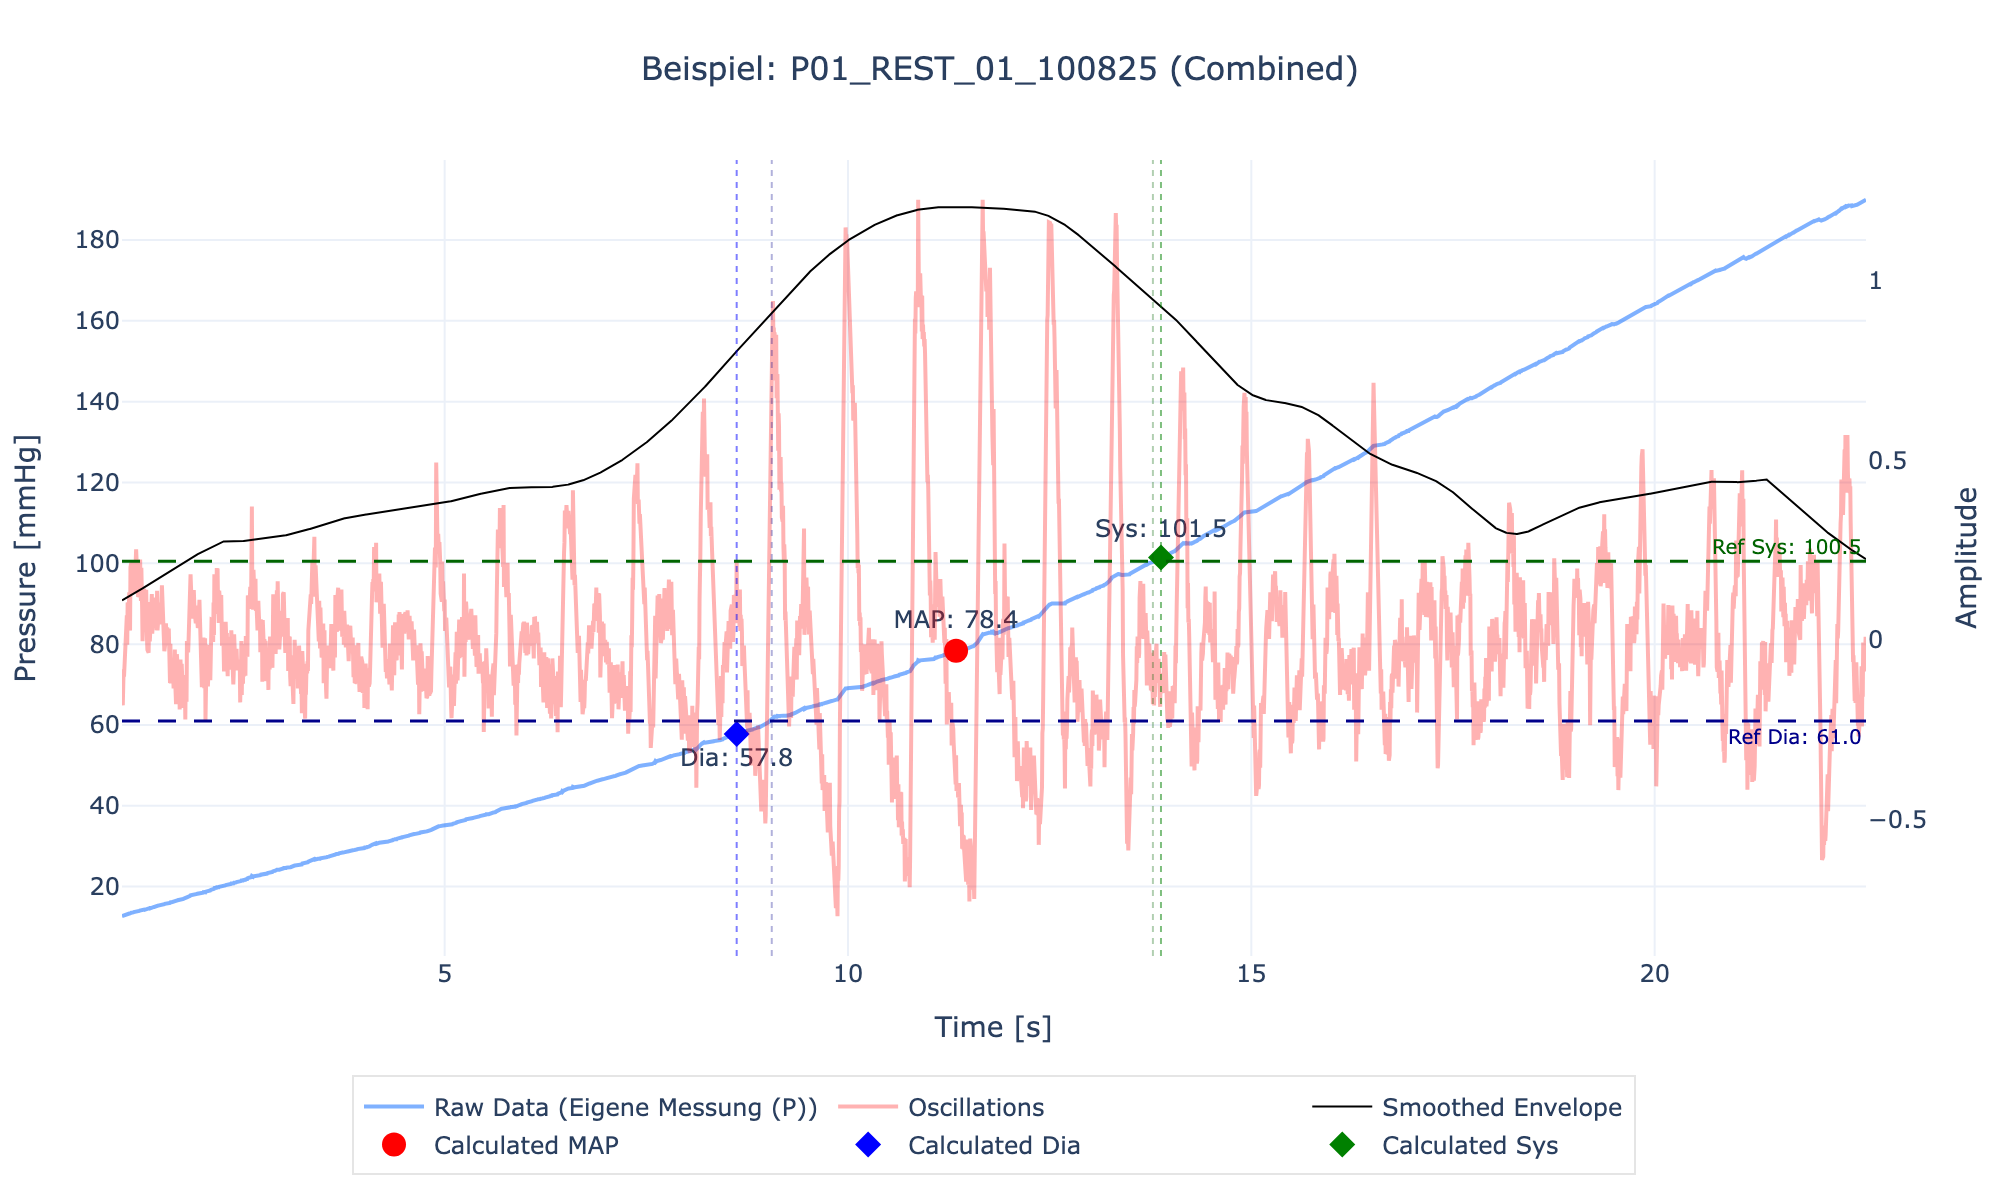
\includegraphics[width=0.9\textwidth]{images/extraktion-beispiel.png}
    \caption{Signalverarbeitungsschritte: Originalsignal (blau), Druckrampe (grün), oszillometrisches Signal (rot), PCHIP-Hüllkurve (orange) und geglättete Kurve (schwarz) mit markierten MAP, Systole und Diastole.}
    \label{fig:signal-processing}
\end{figure}

\newpage

\section*{Bestimmung der Übereinstimmung mit den Referenzwerten}
Um die Genauigkeit des Algorithmus zu maximieren, wurde ein systematischer Ansatz zur Parameterwahl gewählt. Da der Algorithmus insgesamt neun einstellbare Parameter besitzt (Filterordnungen, Grenzfrequenzen, Glättungsfenster und MAA-Schwellenwerte), wurde eine automatisierte Suche im Parameterraum durchgeführt.

\subsection*{Optimierung mit Optuna}
Hierfür wurde das Framework \textit{Optuna} verwendet, welches mittels \textit{Tree-structured Parzen Estimator} (TPE) effizient das globale Optimum findet. Als Zielfunktion (\textit{Objective Function}) wurde eine Kombination aus dem mittleren absoluten Fehler (MAE) und der Standardabweichung der Fehler (SD) gegenüber den Referenzgeräten (Beurer und NAIS) minimiert:
\[ \text{Loss} = \text{MAE} + 2 \cdot \text{SD} \]
Die starke Gewichtung der Standardabweichung stellt sicher, dass der Algorithmus nicht nur im Durchschnitt korrekt ist, sondern eine hohe Konsistenz über verschiedene Probanden und Kreislaufzustände hinweg aufweist.

\subsection*{Einbeziehung zusätzlicher Messdaten}
Zusätzlich zu unseren eigenen 10 Messreihen wurden die Datensätze der Kommilitonen Ziyi und Hanna in die Analyse einbezogen. Dies erhöht die statistische Signifikanz und erlaubt eine robustere Validierung des Algorithmus an einer größeren Diversität von Signalqualitäten und physiologischen Profilen.

\subsection*{Optimierungsergebnisse}
Die automatische Suche mittels Optuna lieferte für die verschiedenen Referenzszenarien unterschiedliche Parametersätze. In Tabelle \ref{tab:parameter-ergebnisse} sind die finalen Werte zusammengefasst, die für die weiteren Auswertungen und die Erstellung des Anhangs verwendet wurden.

\begin{table}[H]
\centering
\begin{tabular}{|l|c|c|c|}
\hline
\textbf{Parameter} & \textbf{Kombiniert} & \textbf{Beurer} & \textbf{NAIS} \\ \hline
$begin\_index$ [s] & 1 & 1 & 2 \\ \hline
$high\_N$ (HP-Ordnung) & 4 & 3 & 4 \\ \hline
$low\_N$ (TP-Ordnung) & 3 & 4 & 3 \\ \hline
$border\_f$ (Grenzfrequenz) [Hz] & 0,89 & 0,94 & 0,91 \\ \hline
$peaks\_distance$ [Samples] & 119 & 121 & 119 \\ \hline
$window\_size$ [s] & 2,50 & 2,47 & 2,24 \\ \hline
$dia\_treshhold$ (MAA Ratio) & 0,67 & 0,65 & 0,67 \\ \hline
$sys\_trashhold$ (MAA Ratio) & 0,77 & 0,78 & 0,77 \\ \hline
\end{tabular}
\caption{Finale optimierte Parameter für die drei verschiedenen Referenz-Szenarien.}
\label{tab:parameter-ergebnisse}
\end{table}

\subsection*{Statistische Auswertung (Bland-Altman)}
Die Übereinstimmung zwischen dem entwickelten Algorithmus und den kommerziellen Referenzgeräten wurde mittels Bland-Altman-Diagrammen visualisiert. Diese Methode erlaubt es, systematische Messabweichungen (\textit{Bias}) sowie die Grenzen der Übereinstimmung (\textit{Limits of Agreement}, $\pm 1.96 \cdot \text{SD}$) direkt abzulesen \cite{Statistical}.

Wir haben die Parameter-Optimierung dreimal durchgeführt und für jedes Szenario die Übereinstimmung analysiert:

\begin{figure}[H]
    \centering
    \begin{subfigure}[b]{0.48\textwidth}
        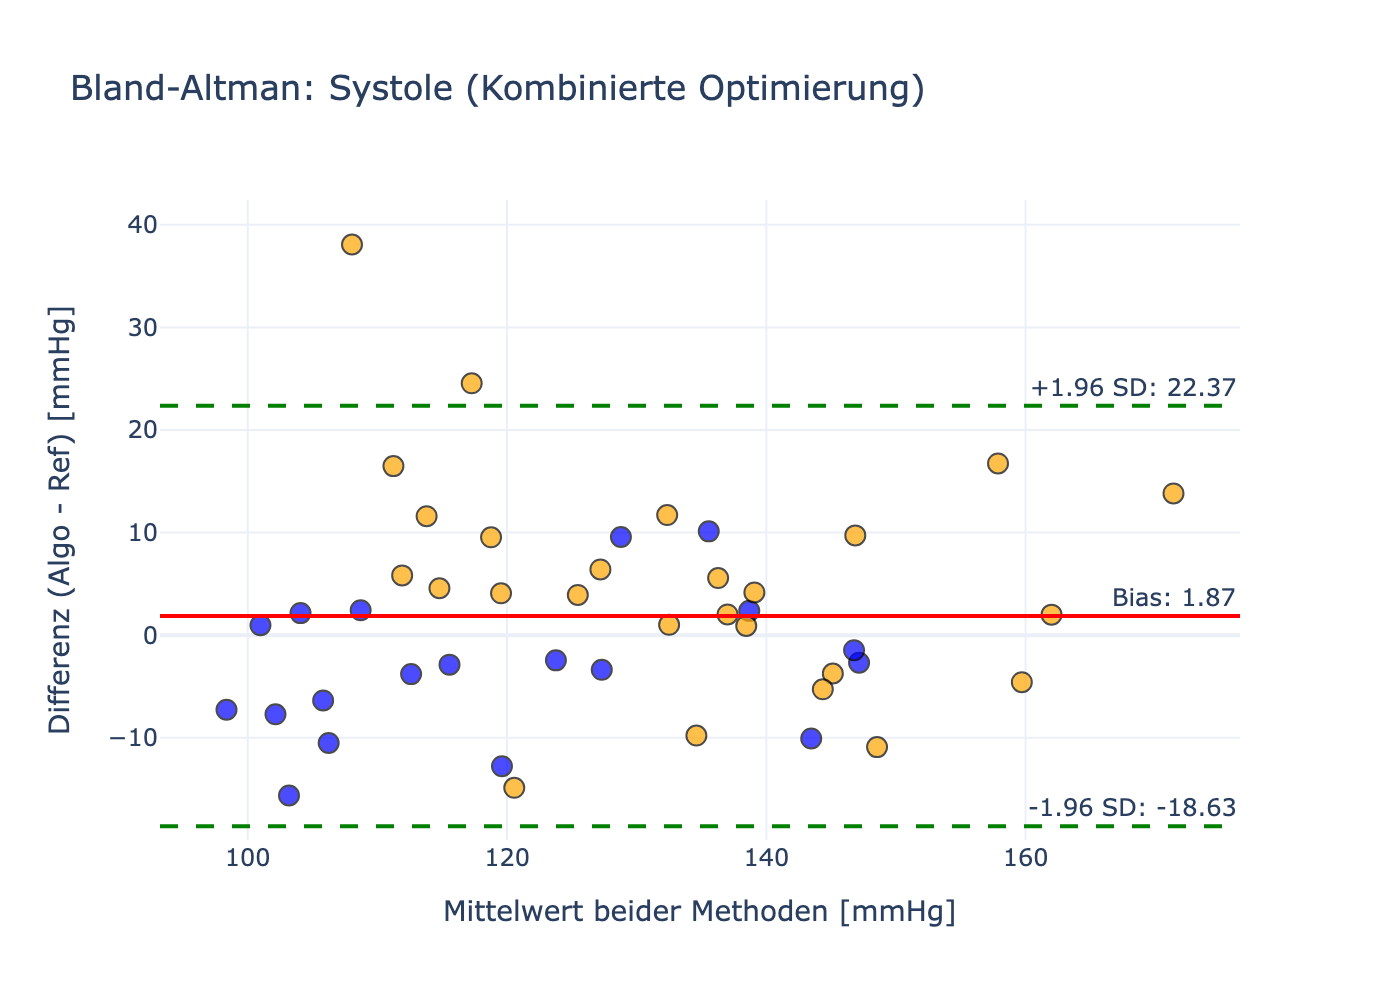
\includegraphics[width=\textwidth]{images/bland-altman-sys.png}
        \caption{Systole (Kombinierte Optimierung)}
    \end{subfigure}
    \hfill
    \begin{subfigure}[b]{0.48\textwidth}
        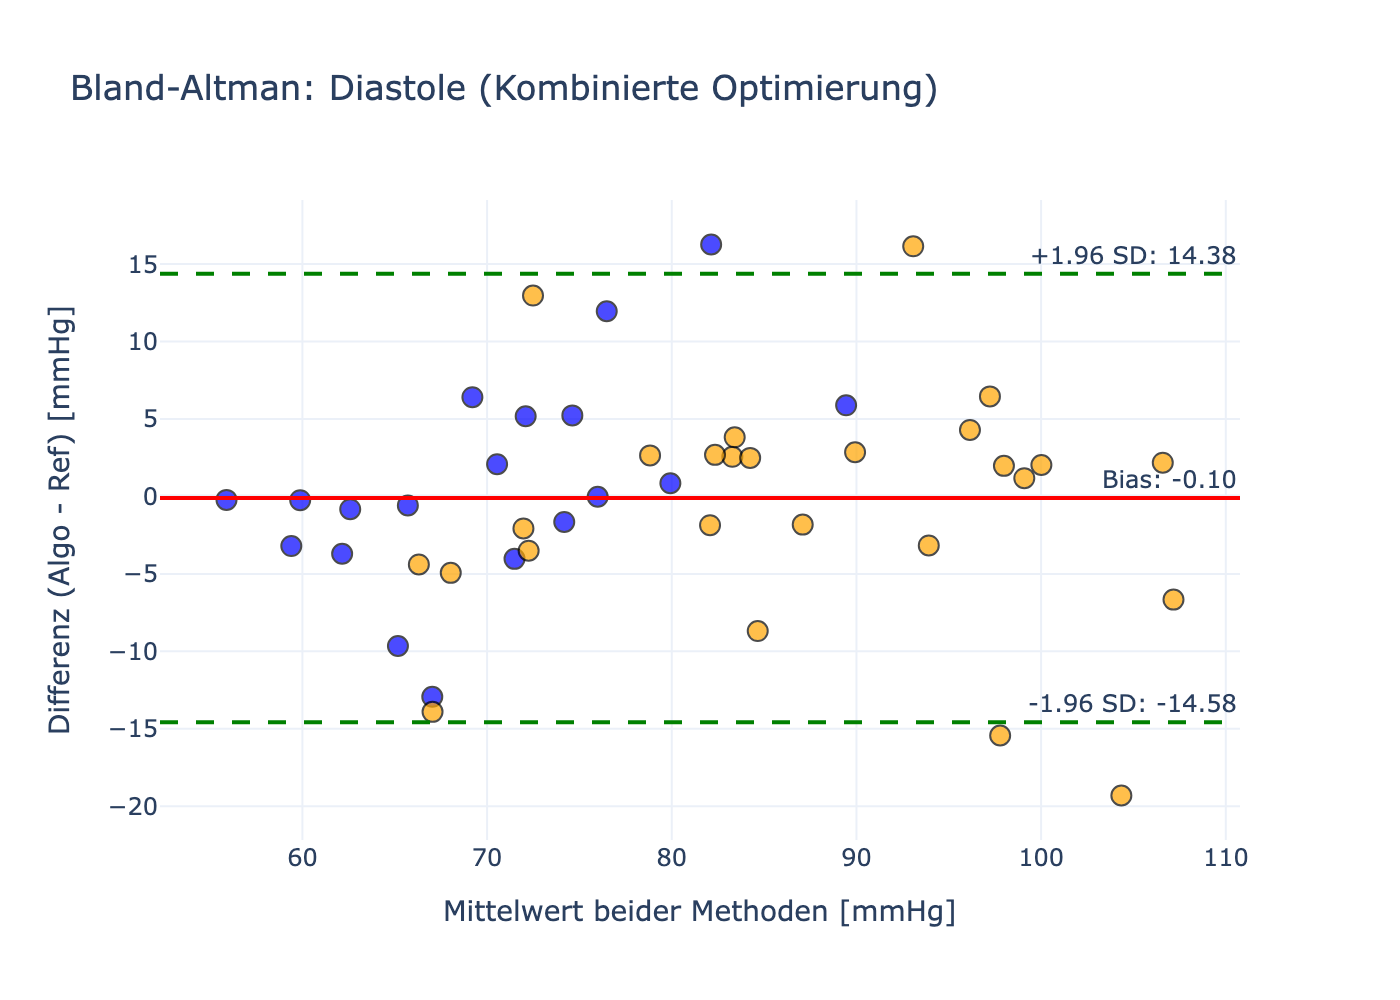
\includegraphics[width=\textwidth]{images/bland-altman-dia.png}
        \caption{Diastole (Kombinierte Optimierung)}
    \end{subfigure}
    \caption{Bland-Altman-Plots: Algorithmus (kombiniert optimiert) vs. Mittelwert der Referenzgeräte.}
    \label{fig:bland-altman-combined}
\end{figure}

\begin{figure}[H]
    \centering
    \begin{subfigure}[b]{0.48\textwidth}
        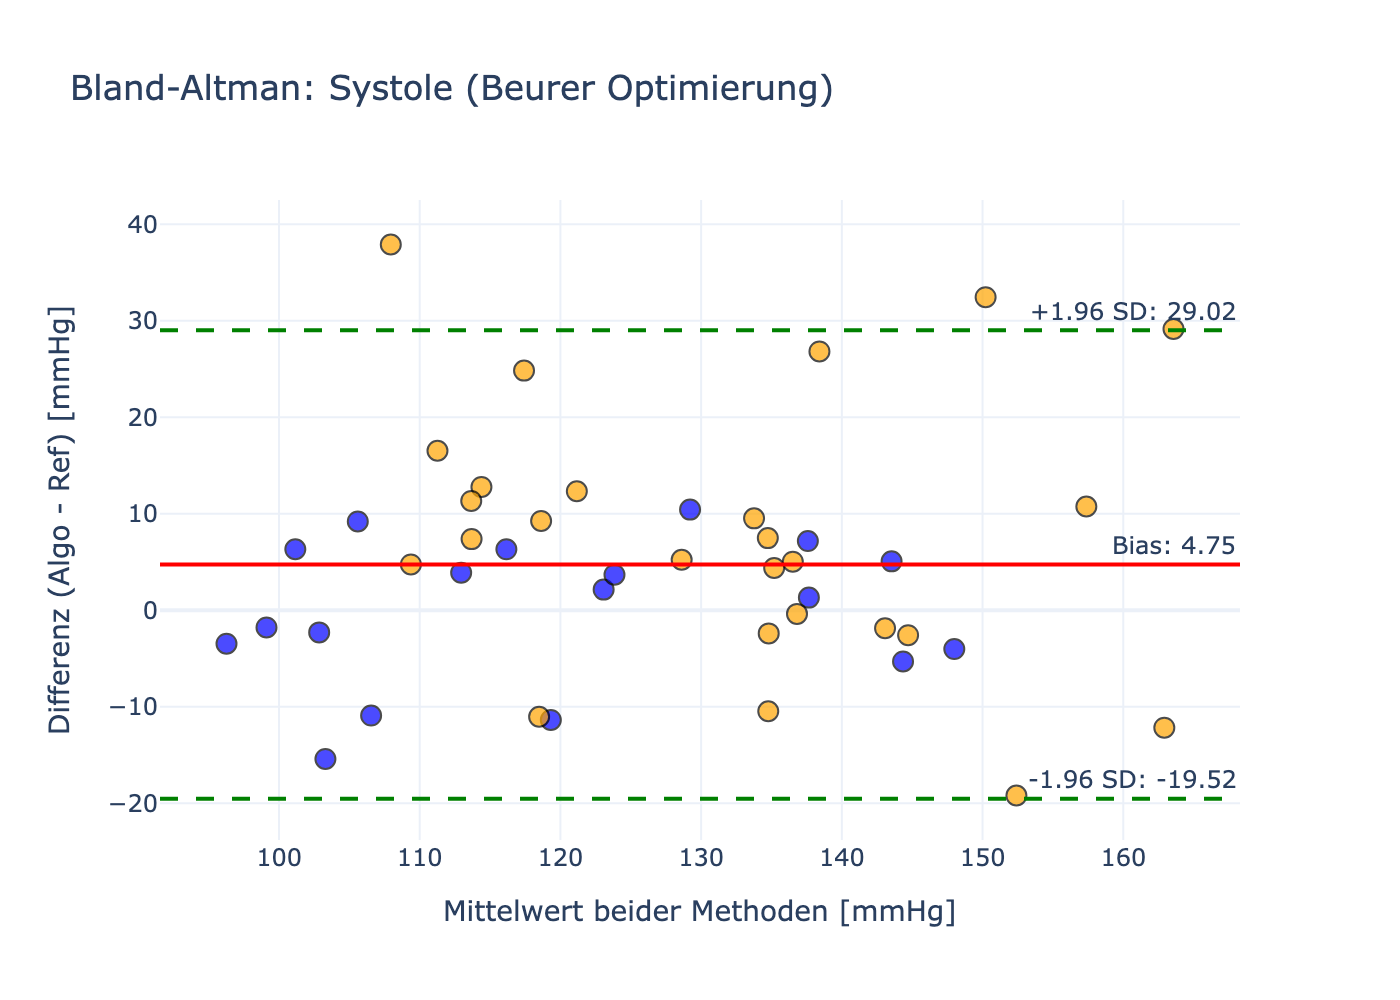
\includegraphics[width=\textwidth]{images/bland-altman-beurer-sys.png}
        \caption{Systole (Beurer Optimierung)}
    \end{subfigure}
    \hfill
    \begin{subfigure}[b]{0.48\textwidth}
        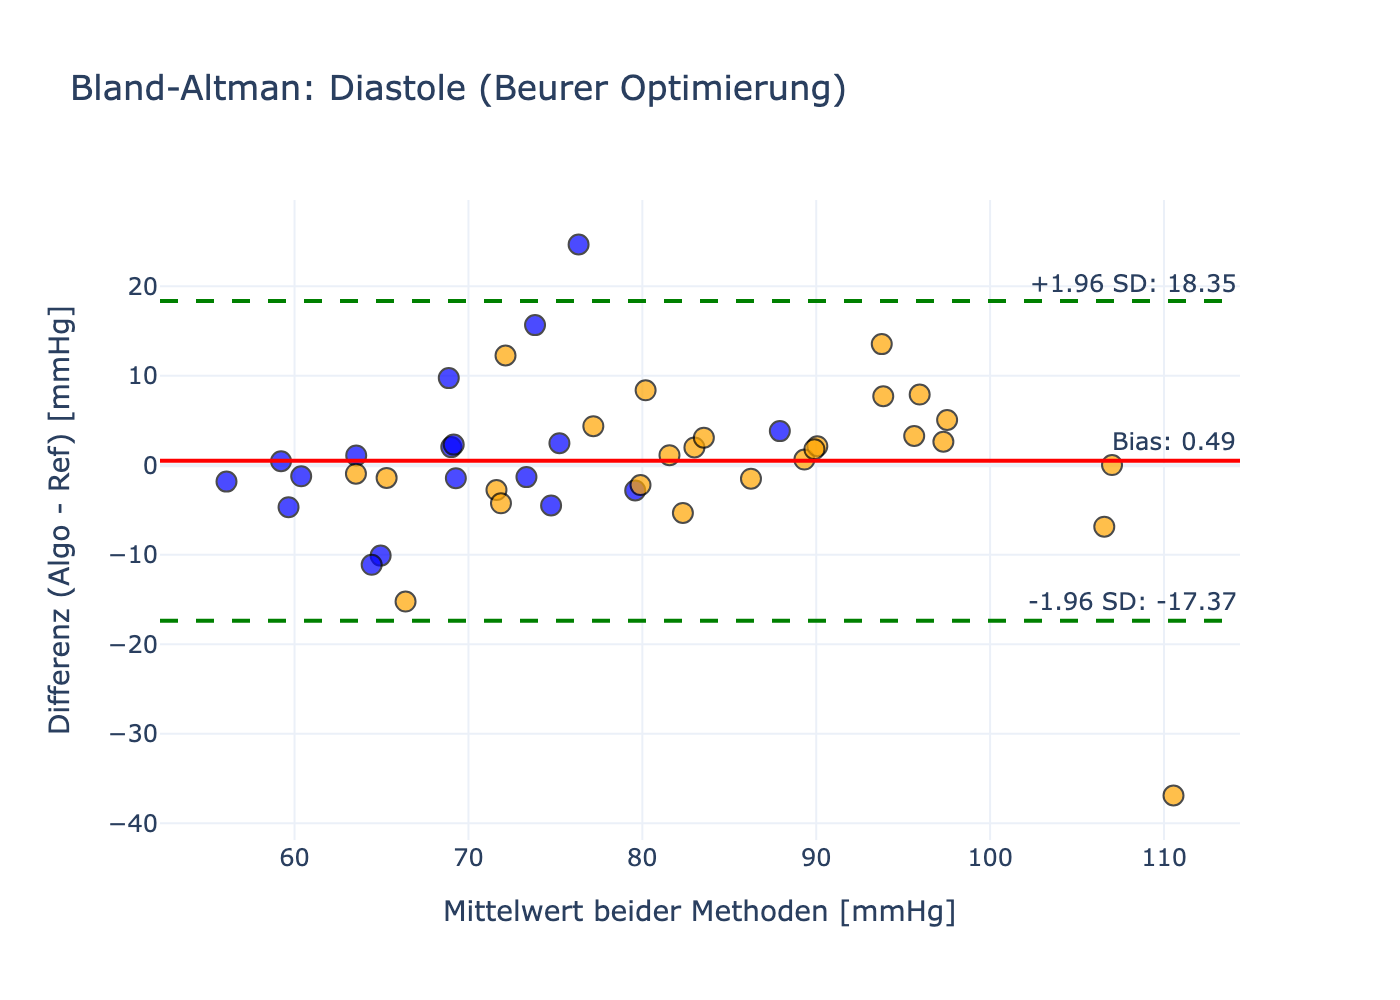
\includegraphics[width=\textwidth]{images/bland-altman-beurer-dia.png}
        \caption{Diastole (Beurer Optimierung)}
    \end{subfigure}
    \caption{Bland-Altman-Plots: Algorithmus (Beurer optimiert) vs. Referenzgerät Beurer.}
    \label{fig:bland-altman-beurer}
\end{figure}

\begin{figure}[H]
    \centering
    \begin{subfigure}[b]{0.48\textwidth}
        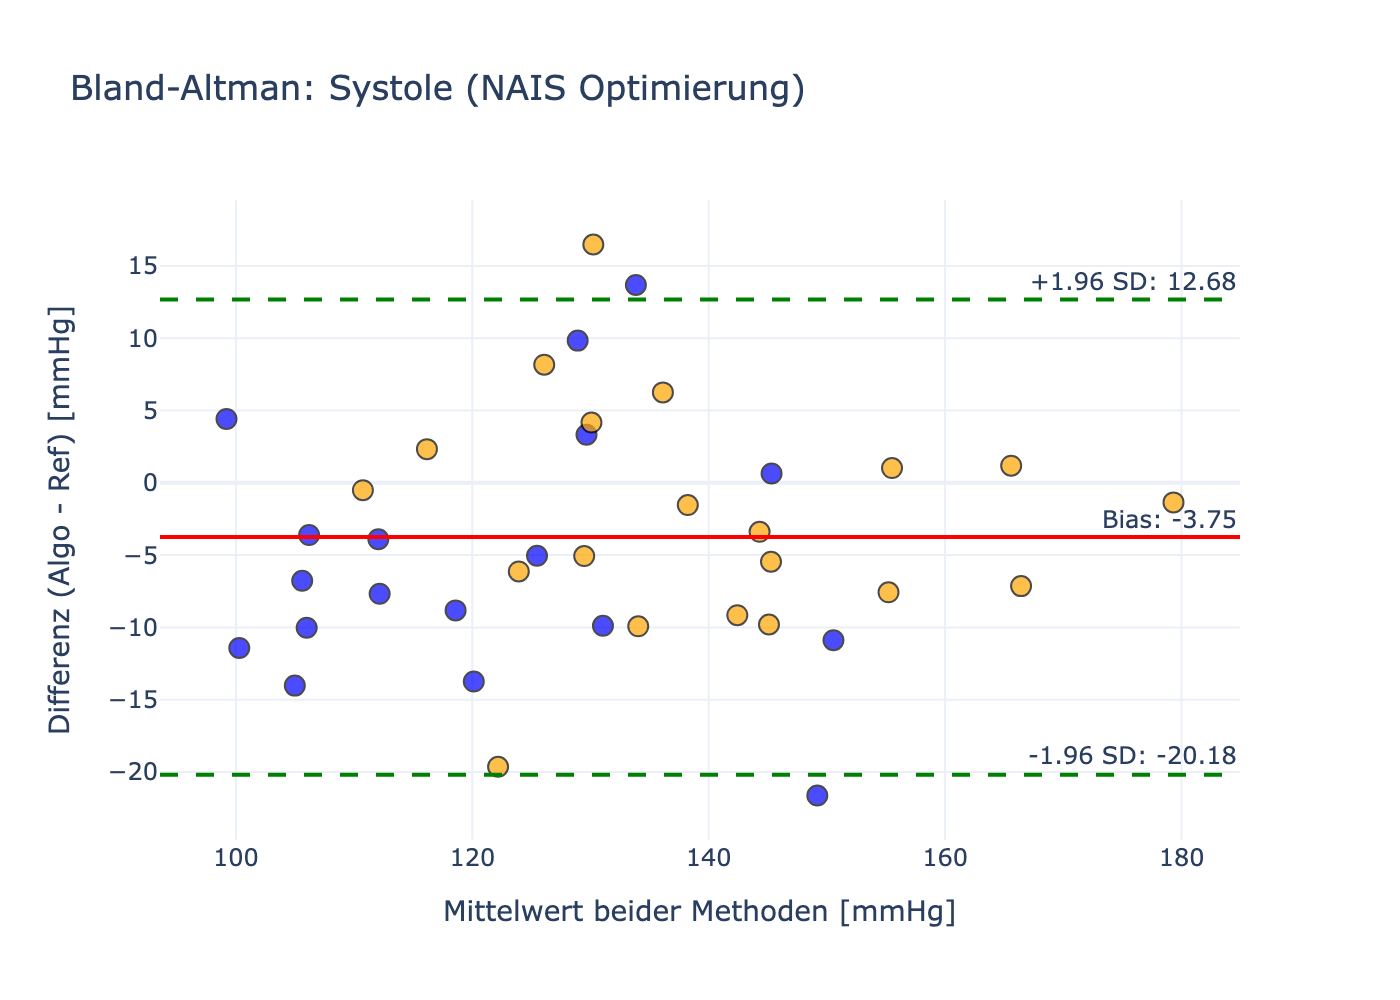
\includegraphics[width=\textwidth]{images/bland-altman-nais-sys.png}
        \caption{Systole (NAIS Optimierung)}
    \end{subfigure}
    \hfill
    \begin{subfigure}[b]{0.48\textwidth}
        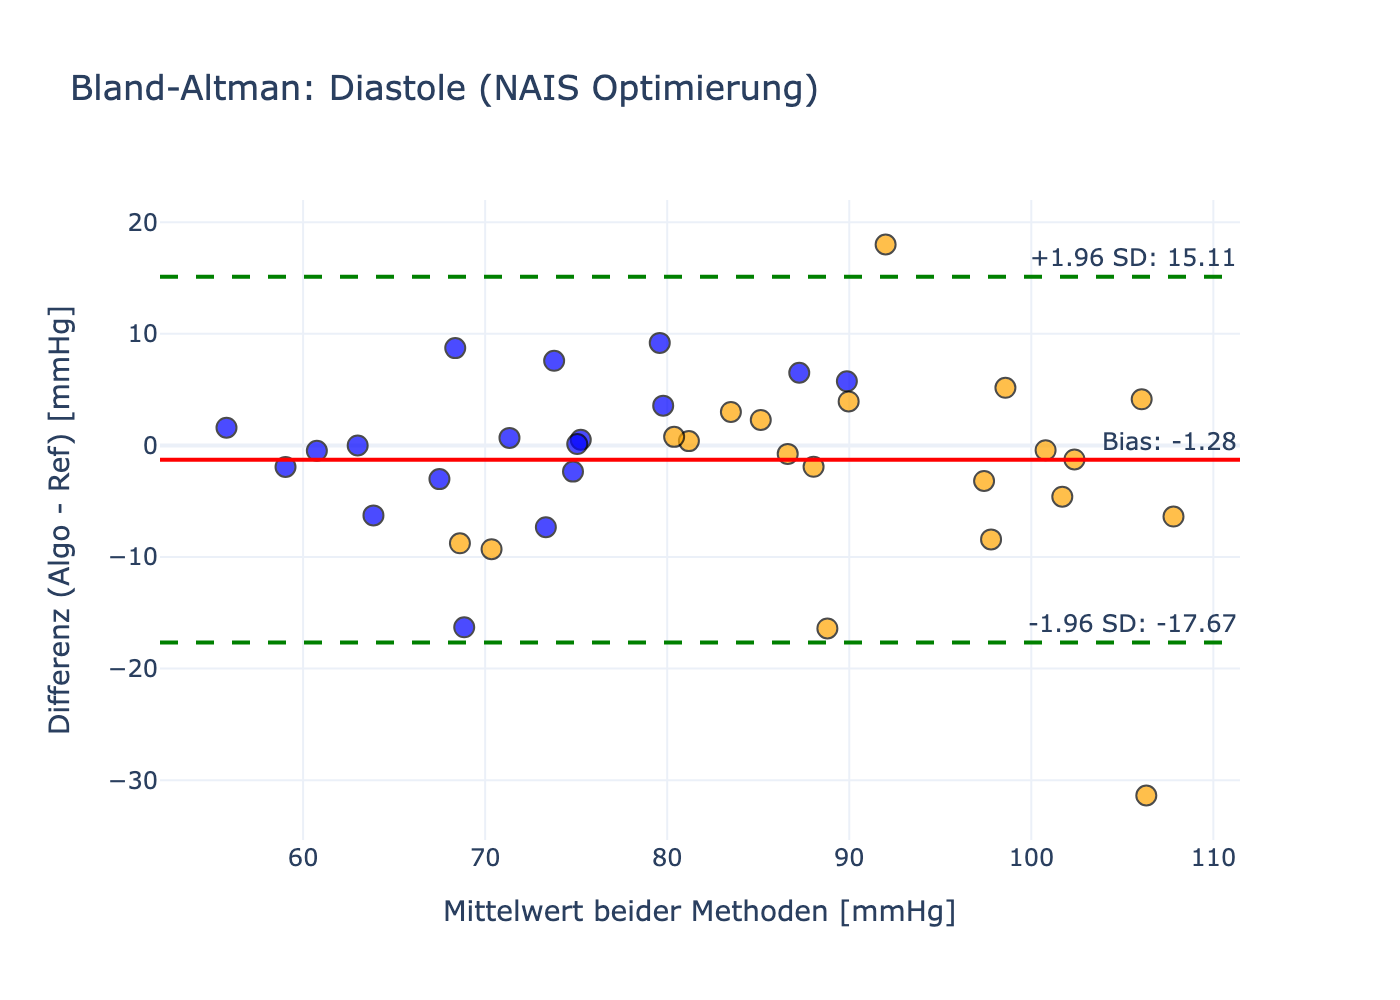
\includegraphics[width=\textwidth]{images/bland-altman-nais-dia.png}
        \caption{Diastole (NAIS Optimierung)}
    \end{subfigure}
    \caption{Bland-Altman-Plots: Algorithmus (NAIS optimiert) vs. Referenzgerät NAIS.}
    \label{fig:bland-altman-nais}
\end{figure}



\newpage

\section{Anhang: Einzelauswertungen}
In diesem Anhang sind die Einzelauswertungen für alle 23 Probanden unter Anwendung der drei verschiedenen Optimierungsszenarien dargestellt.

\subsection*{Messung: P01\_ACTIV\_01\_160925}
\begin{figure}[H]
    \centering
    \begin{subfigure}[b]{0.8\textwidth}
        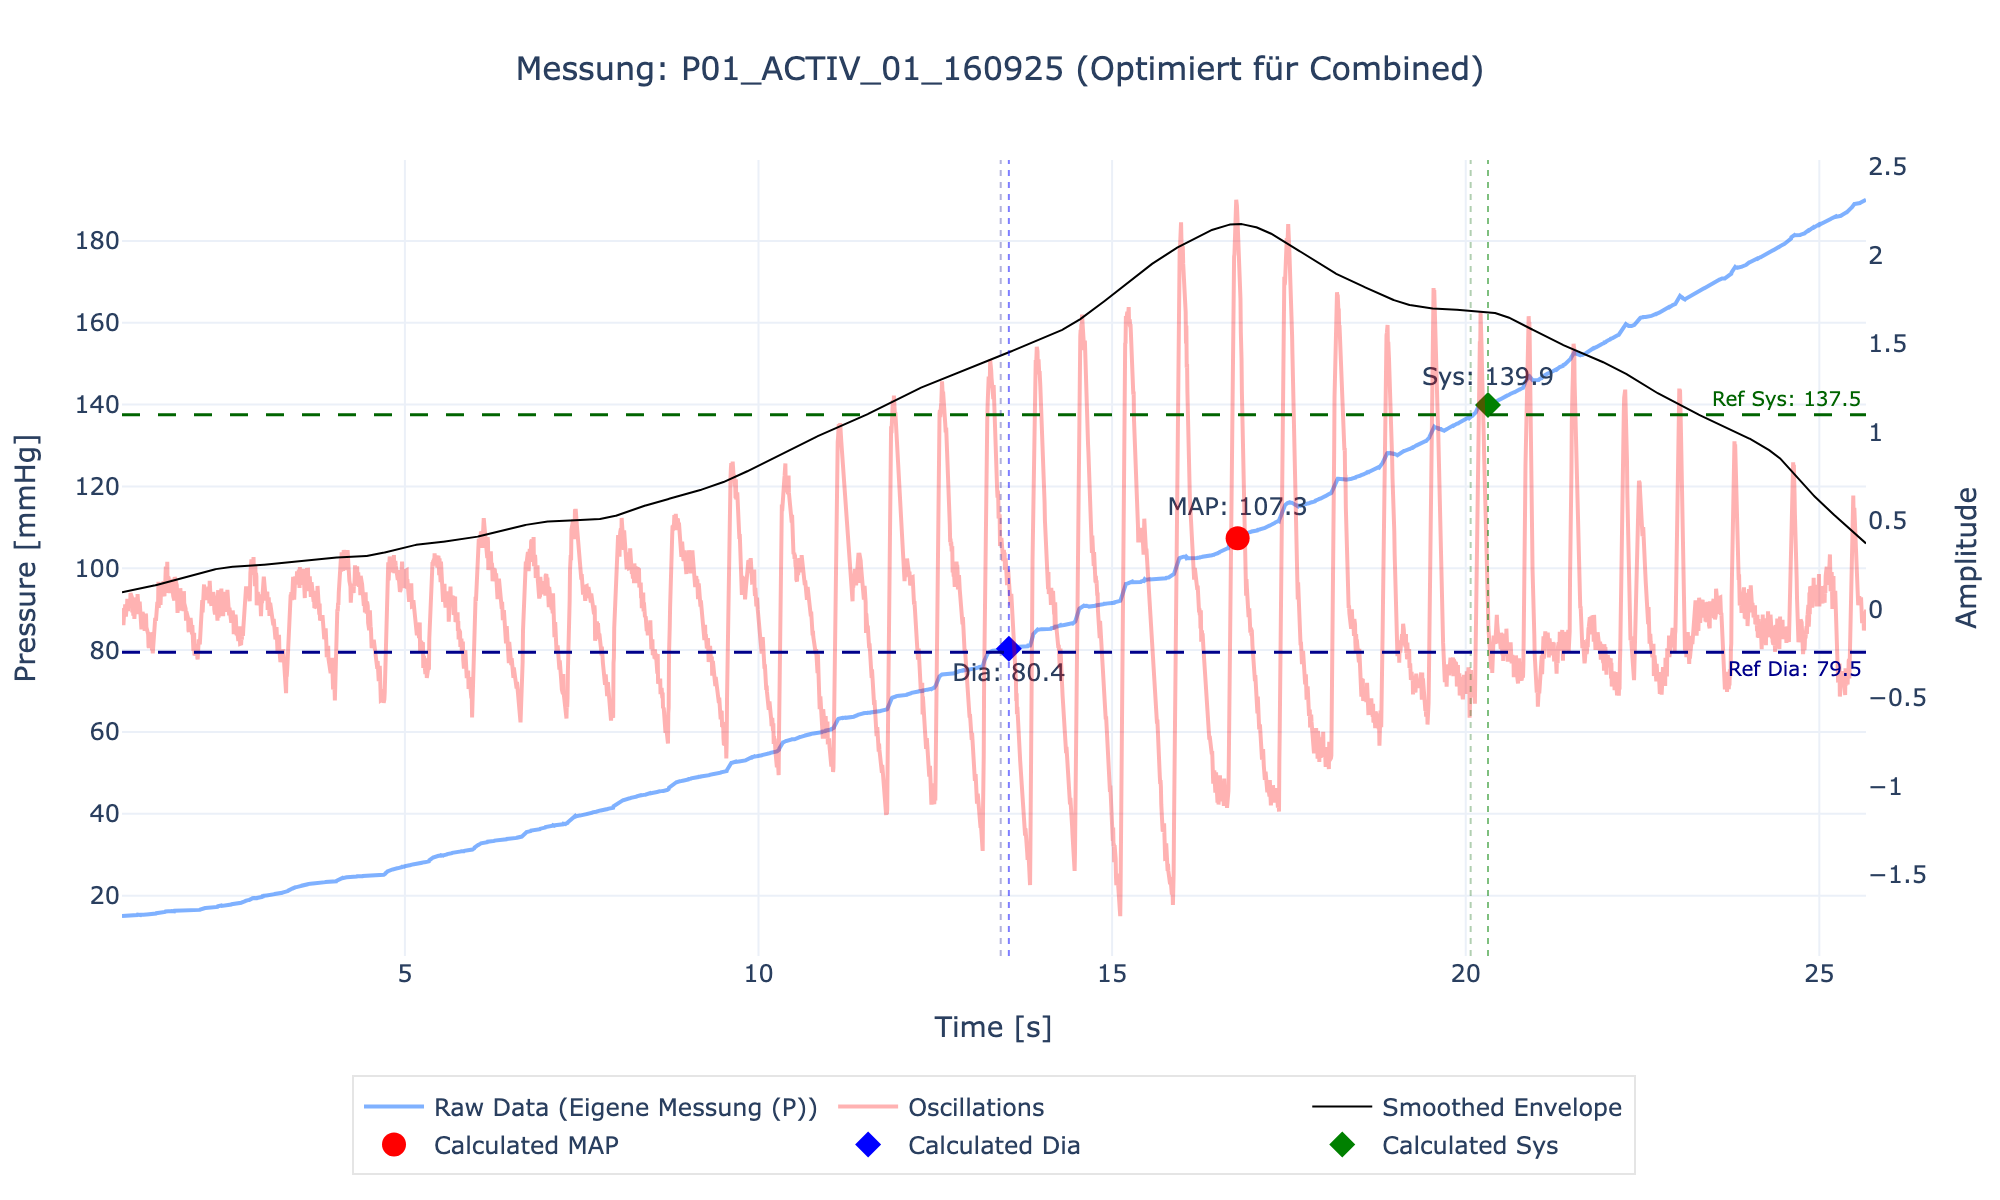
\includegraphics[width=\textwidth]{images/P01_ACTIV_01_160925_combined.png}
        \caption{Optimiert für Beurer und NAIS (Kombiniert)}
    \end{subfigure} \\
    \begin{subfigure}[b]{0.48\textwidth}
        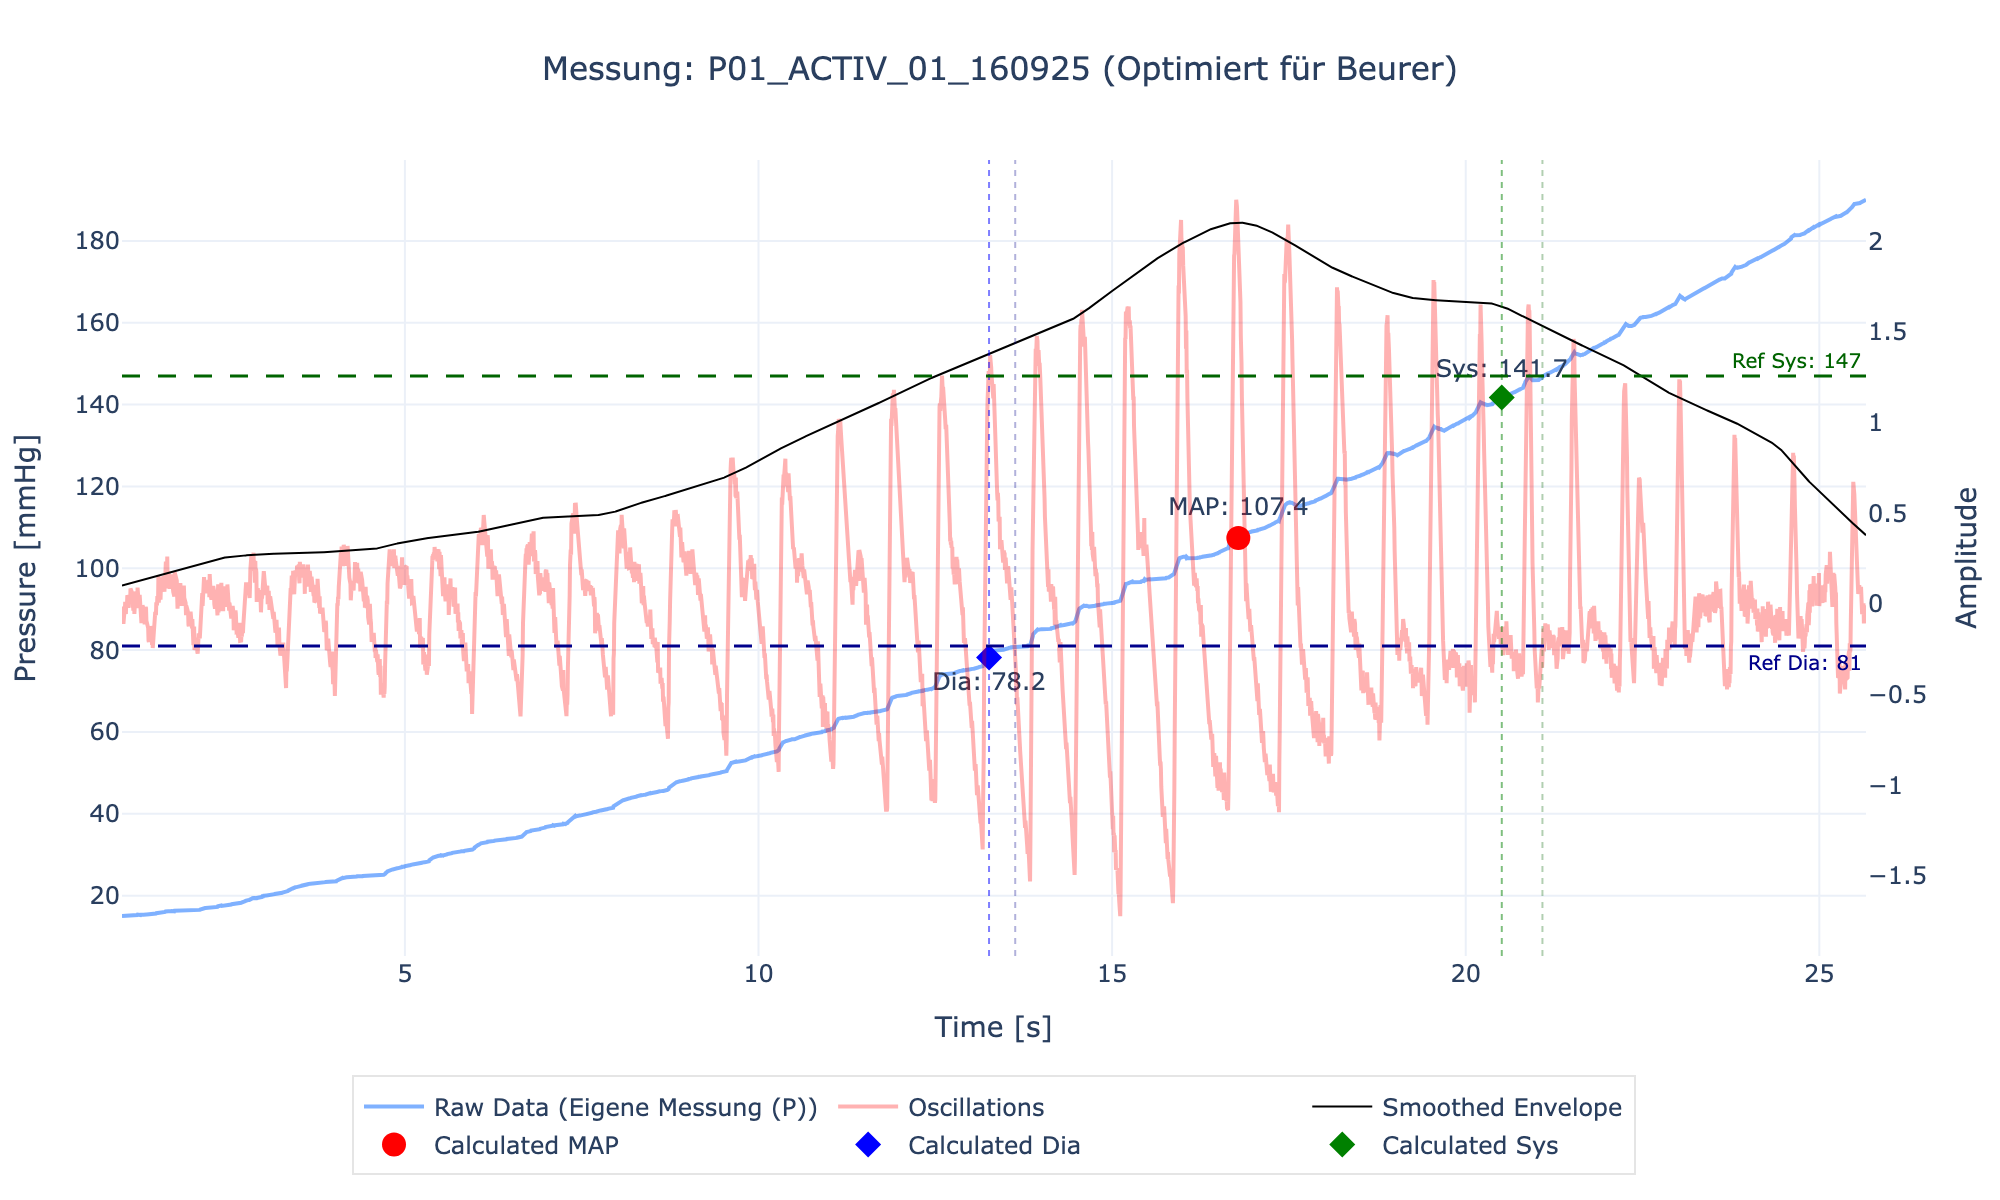
\includegraphics[width=\textwidth]{images/P01_ACTIV_01_160925_beurer.png}
        \caption{Optimiert für Beurer}
    \end{subfigure}
    \hfill
    \begin{subfigure}[b]{0.48\textwidth}
        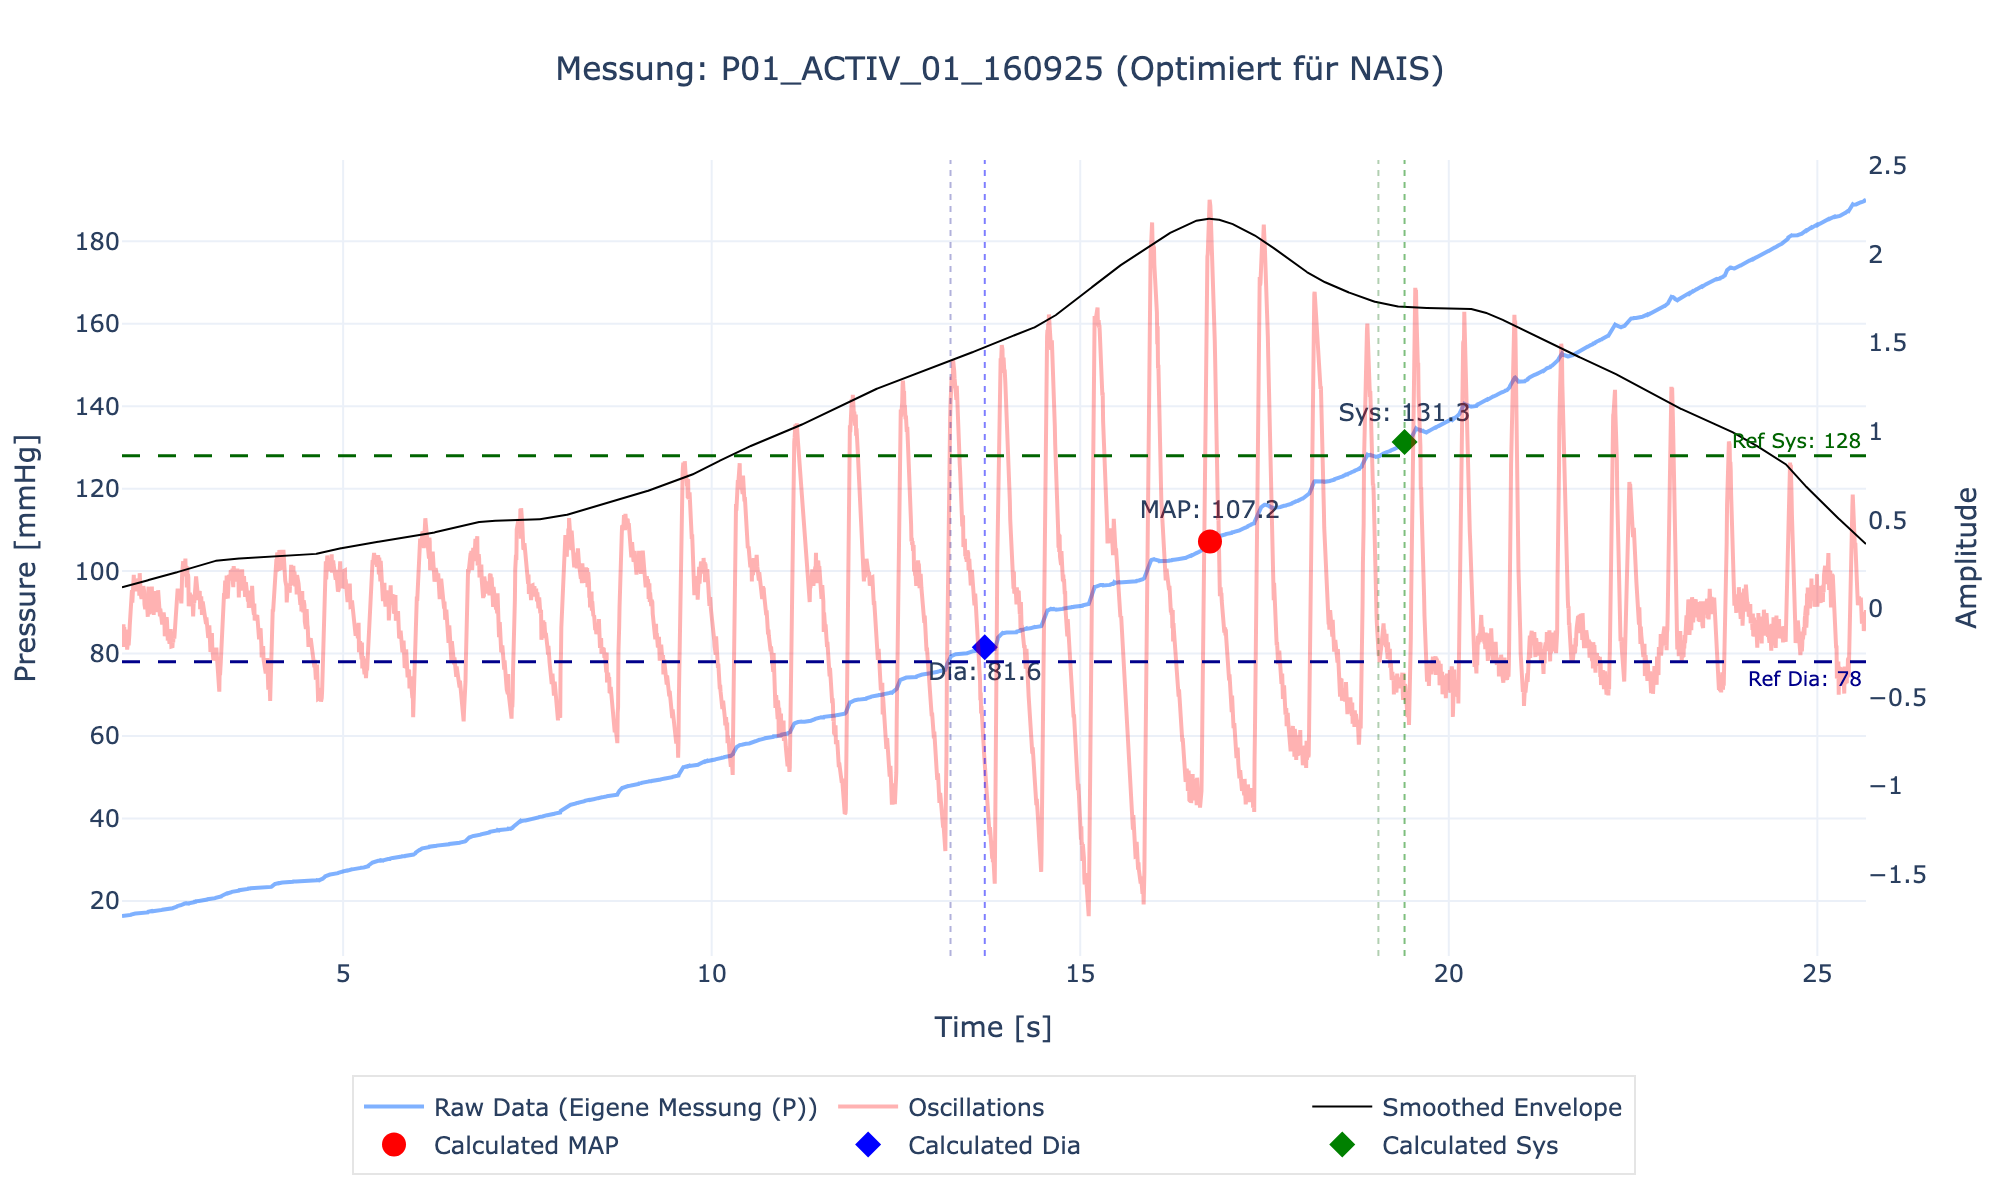
\includegraphics[width=\textwidth]{images/P01_ACTIV_01_160925_nais.png}
        \caption{Optimiert für NAIS}
    \end{subfigure}
    \caption{Einzelauswertung der Messung P01\_ACTIV\_01\_160925 mit verschiedenen Parametersätzen.}
\end{figure}
\newpage

\subsection*{Messung: P01\_REST\_01\_100825}
\begin{figure}[H]
    \centering
    \begin{subfigure}[b]{0.8\textwidth}
        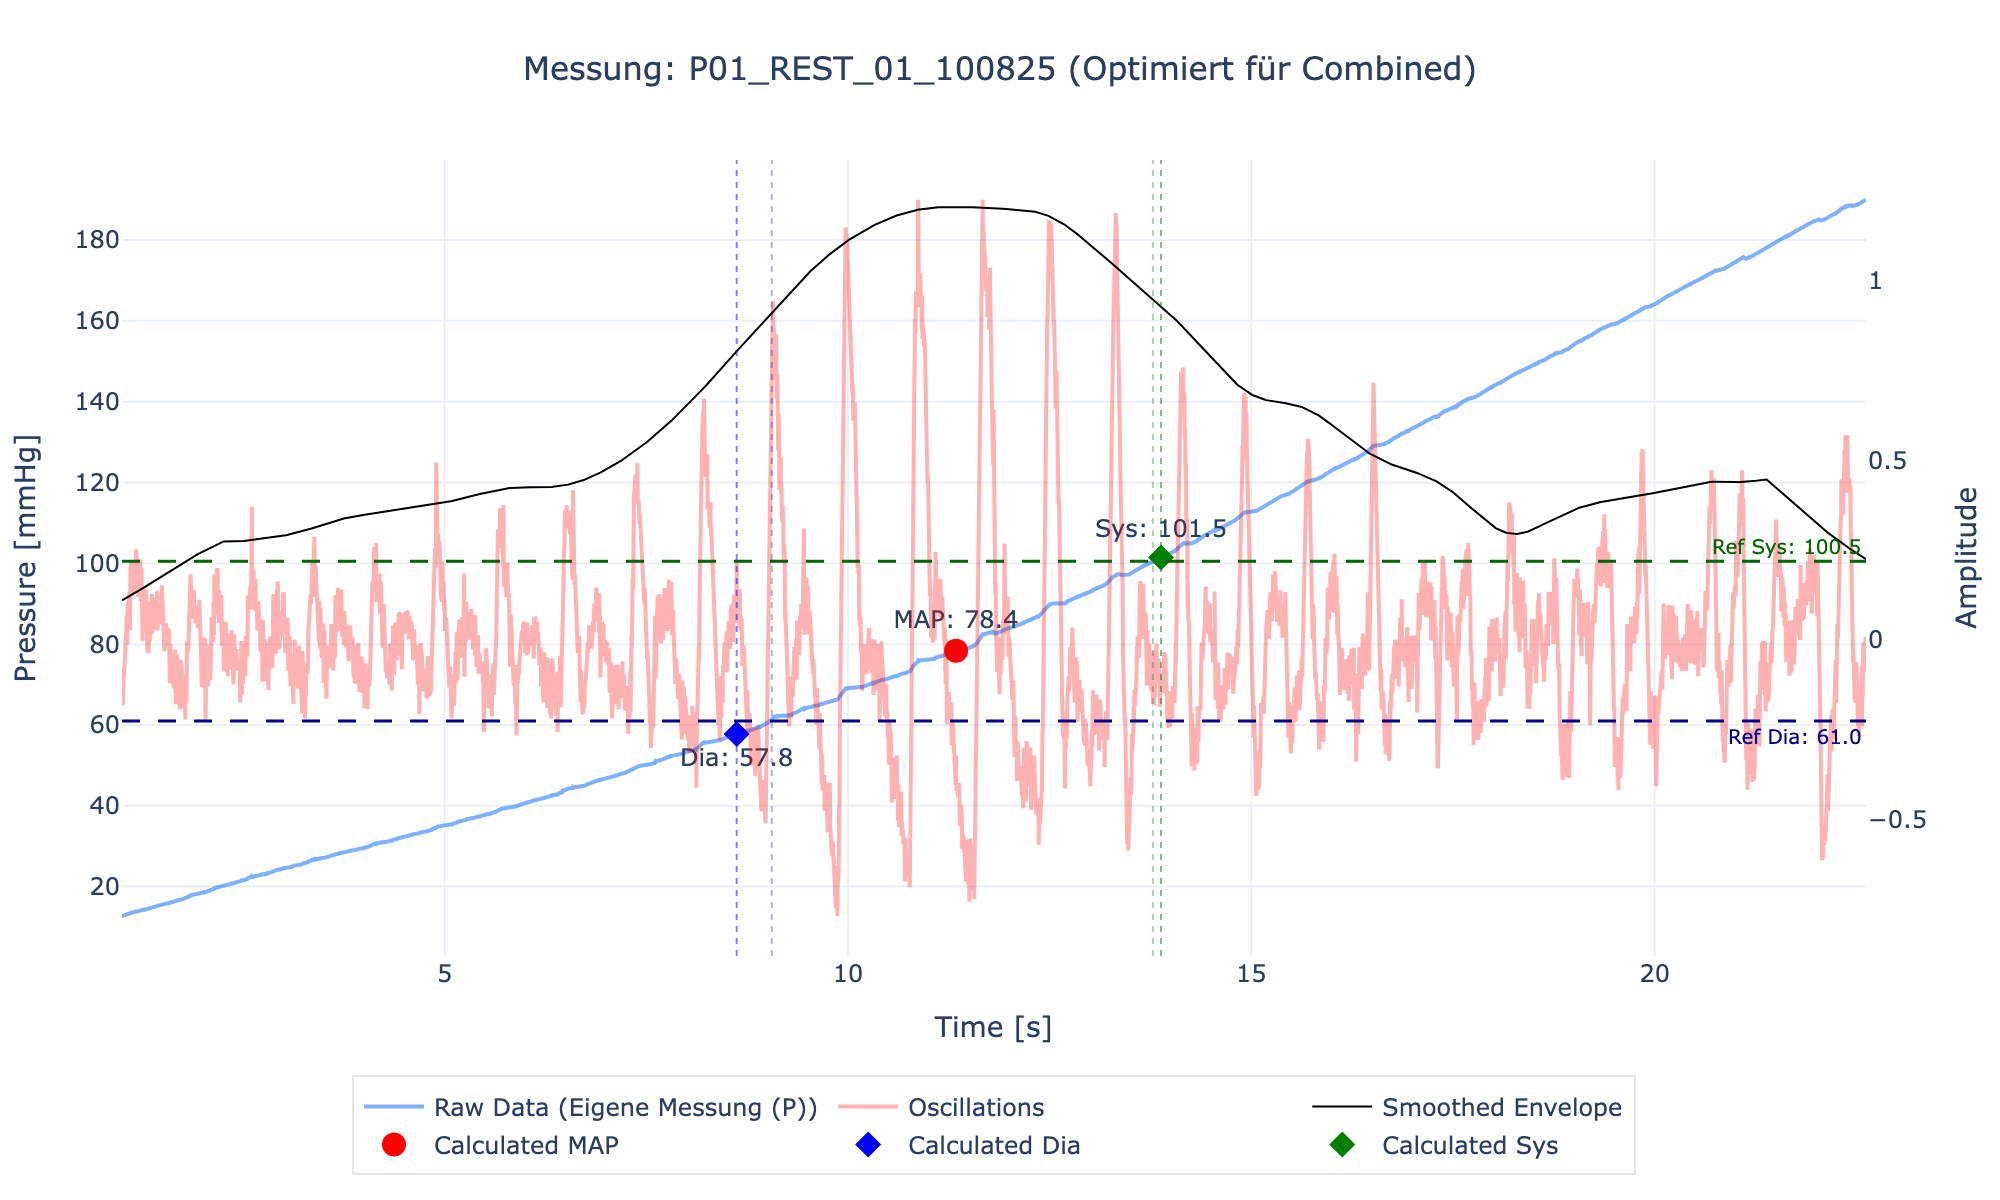
\includegraphics[width=\textwidth]{images/P01_REST_01_100825_combined.png}
        \caption{Optimiert für Beurer und NAIS (Kombiniert)}
    \end{subfigure} \\
    \begin{subfigure}[b]{0.48\textwidth}
        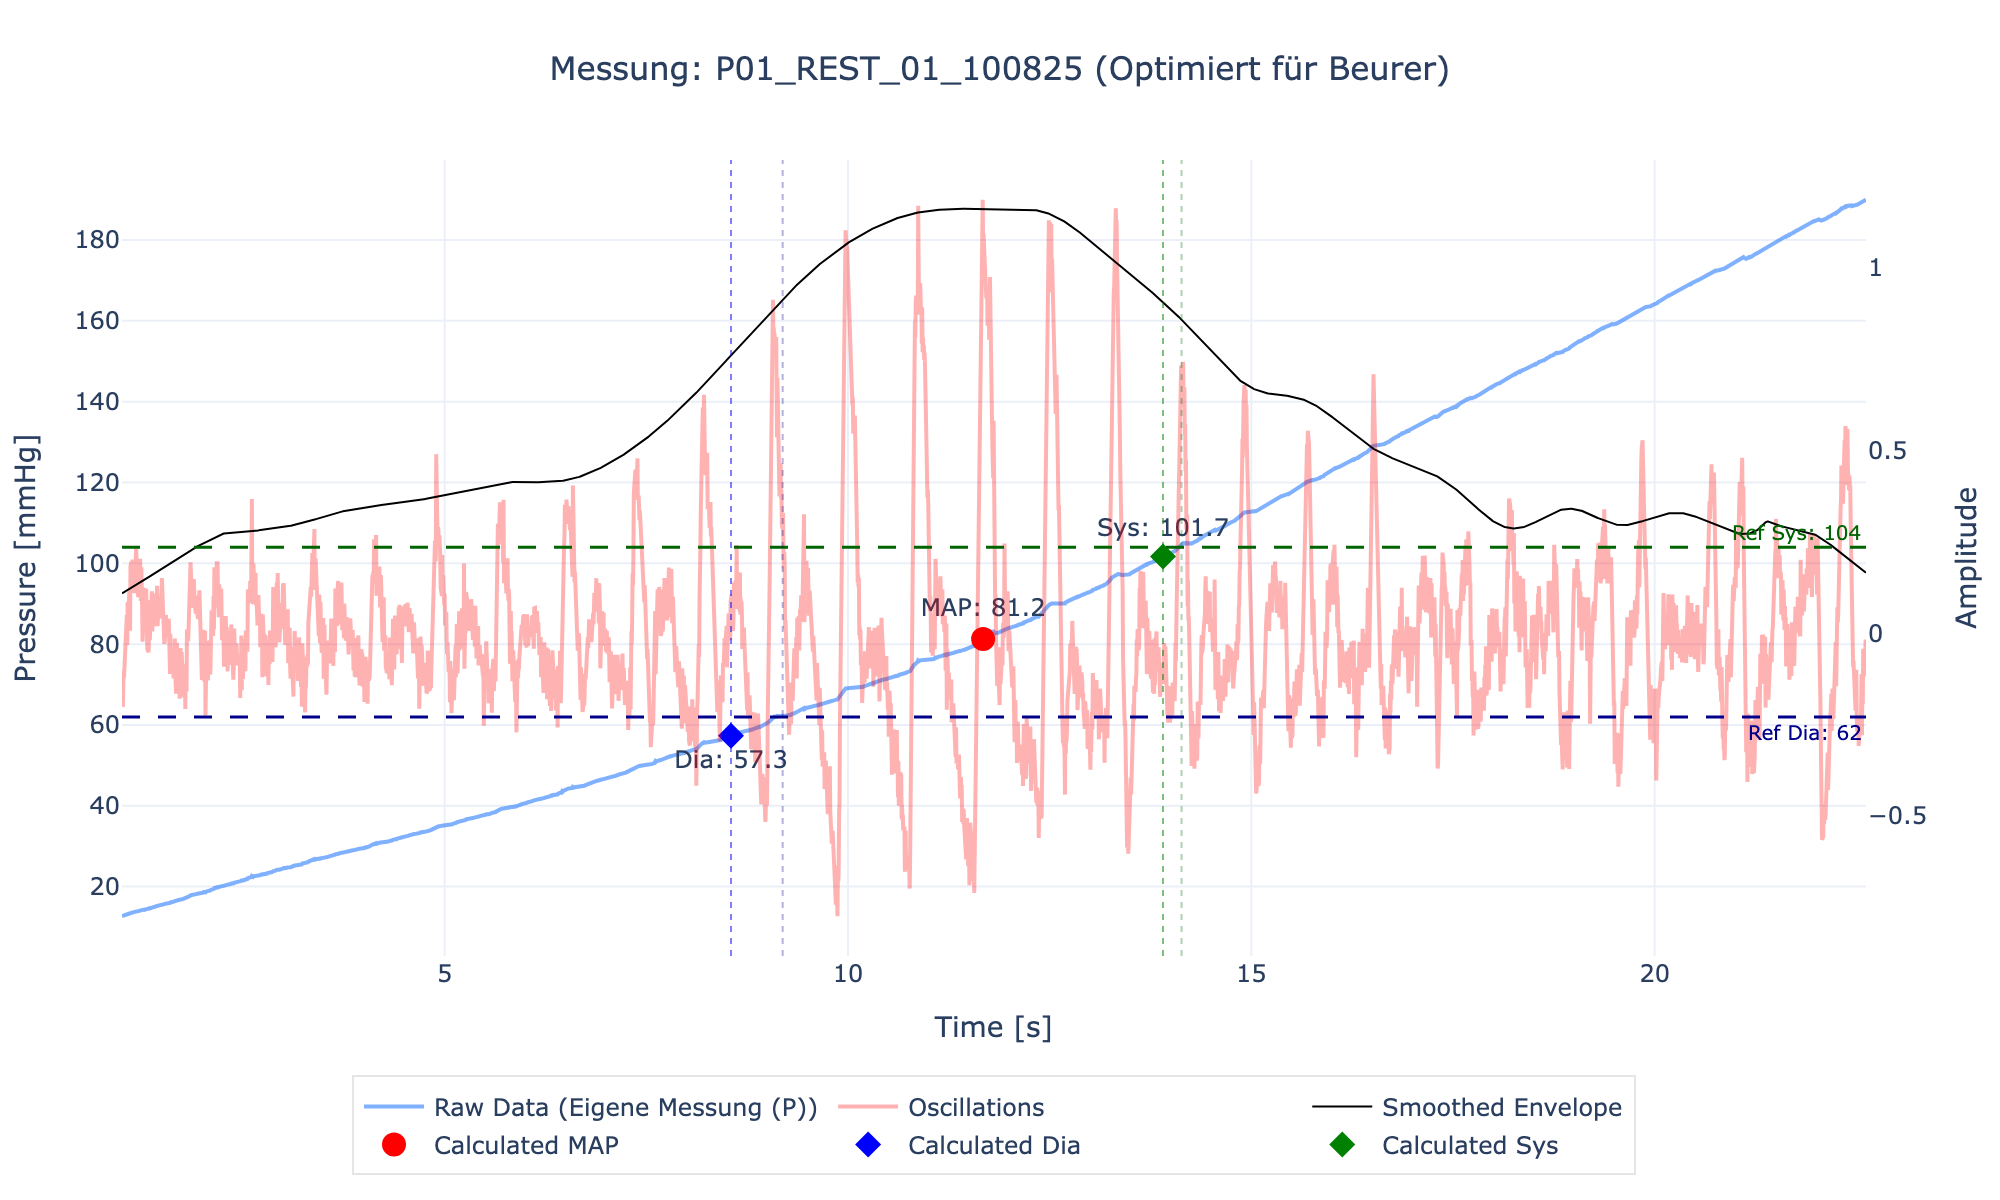
\includegraphics[width=\textwidth]{images/P01_REST_01_100825_beurer.png}
        \caption{Optimiert für Beurer}
    \end{subfigure}
    \hfill
    \begin{subfigure}[b]{0.48\textwidth}
        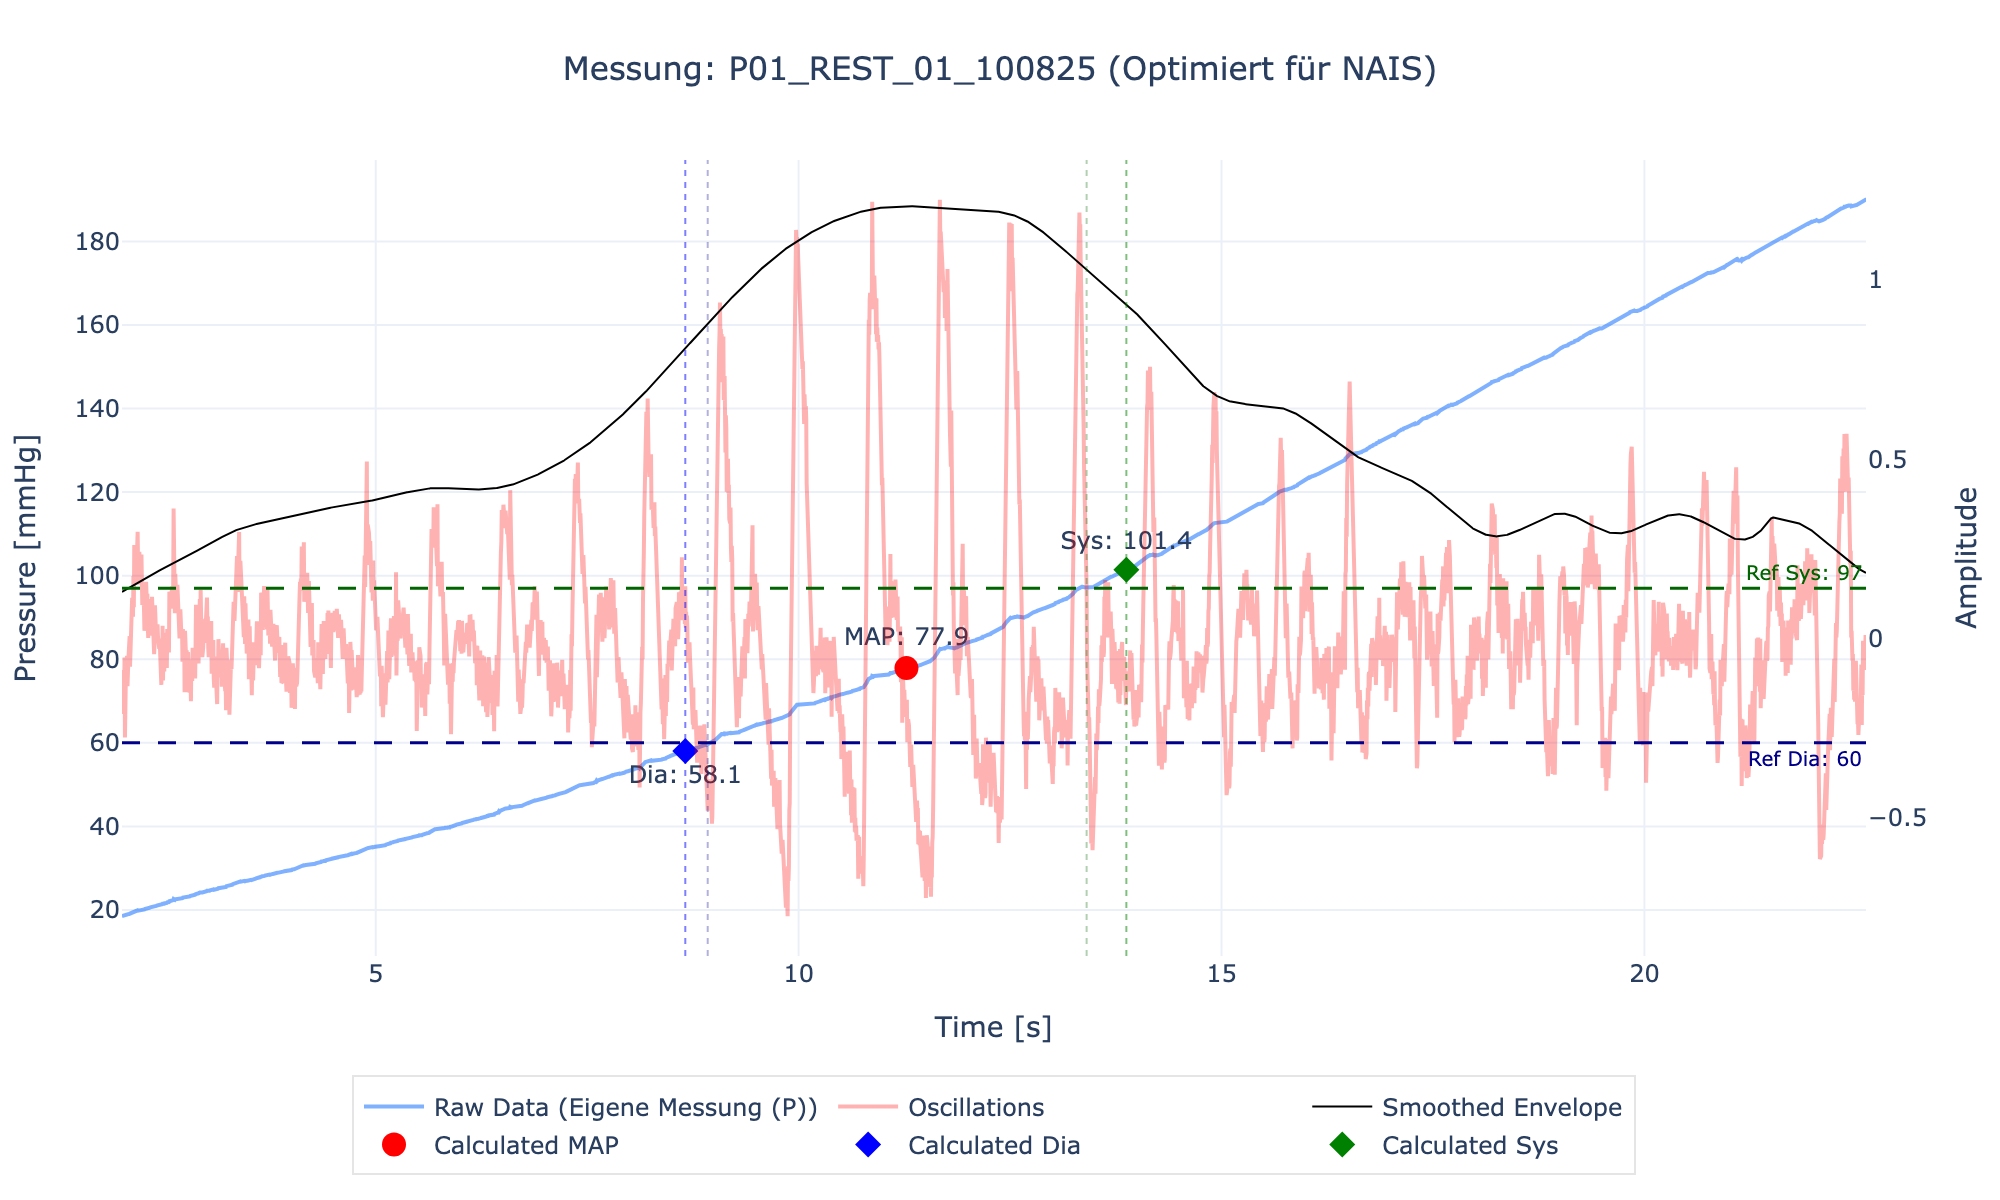
\includegraphics[width=\textwidth]{images/P01_REST_01_100825_nais.png}
        \caption{Optimiert für NAIS}
    \end{subfigure}
    \caption{Einzelauswertung der Messung P01\_REST\_01\_100825 mit verschiedenen Parametersätzen.}
\end{figure}
\newpage

\subsection*{Messung: P01\_REST\_02\_100825}
\begin{figure}[H]
    \centering
    \begin{subfigure}[b]{0.8\textwidth}
        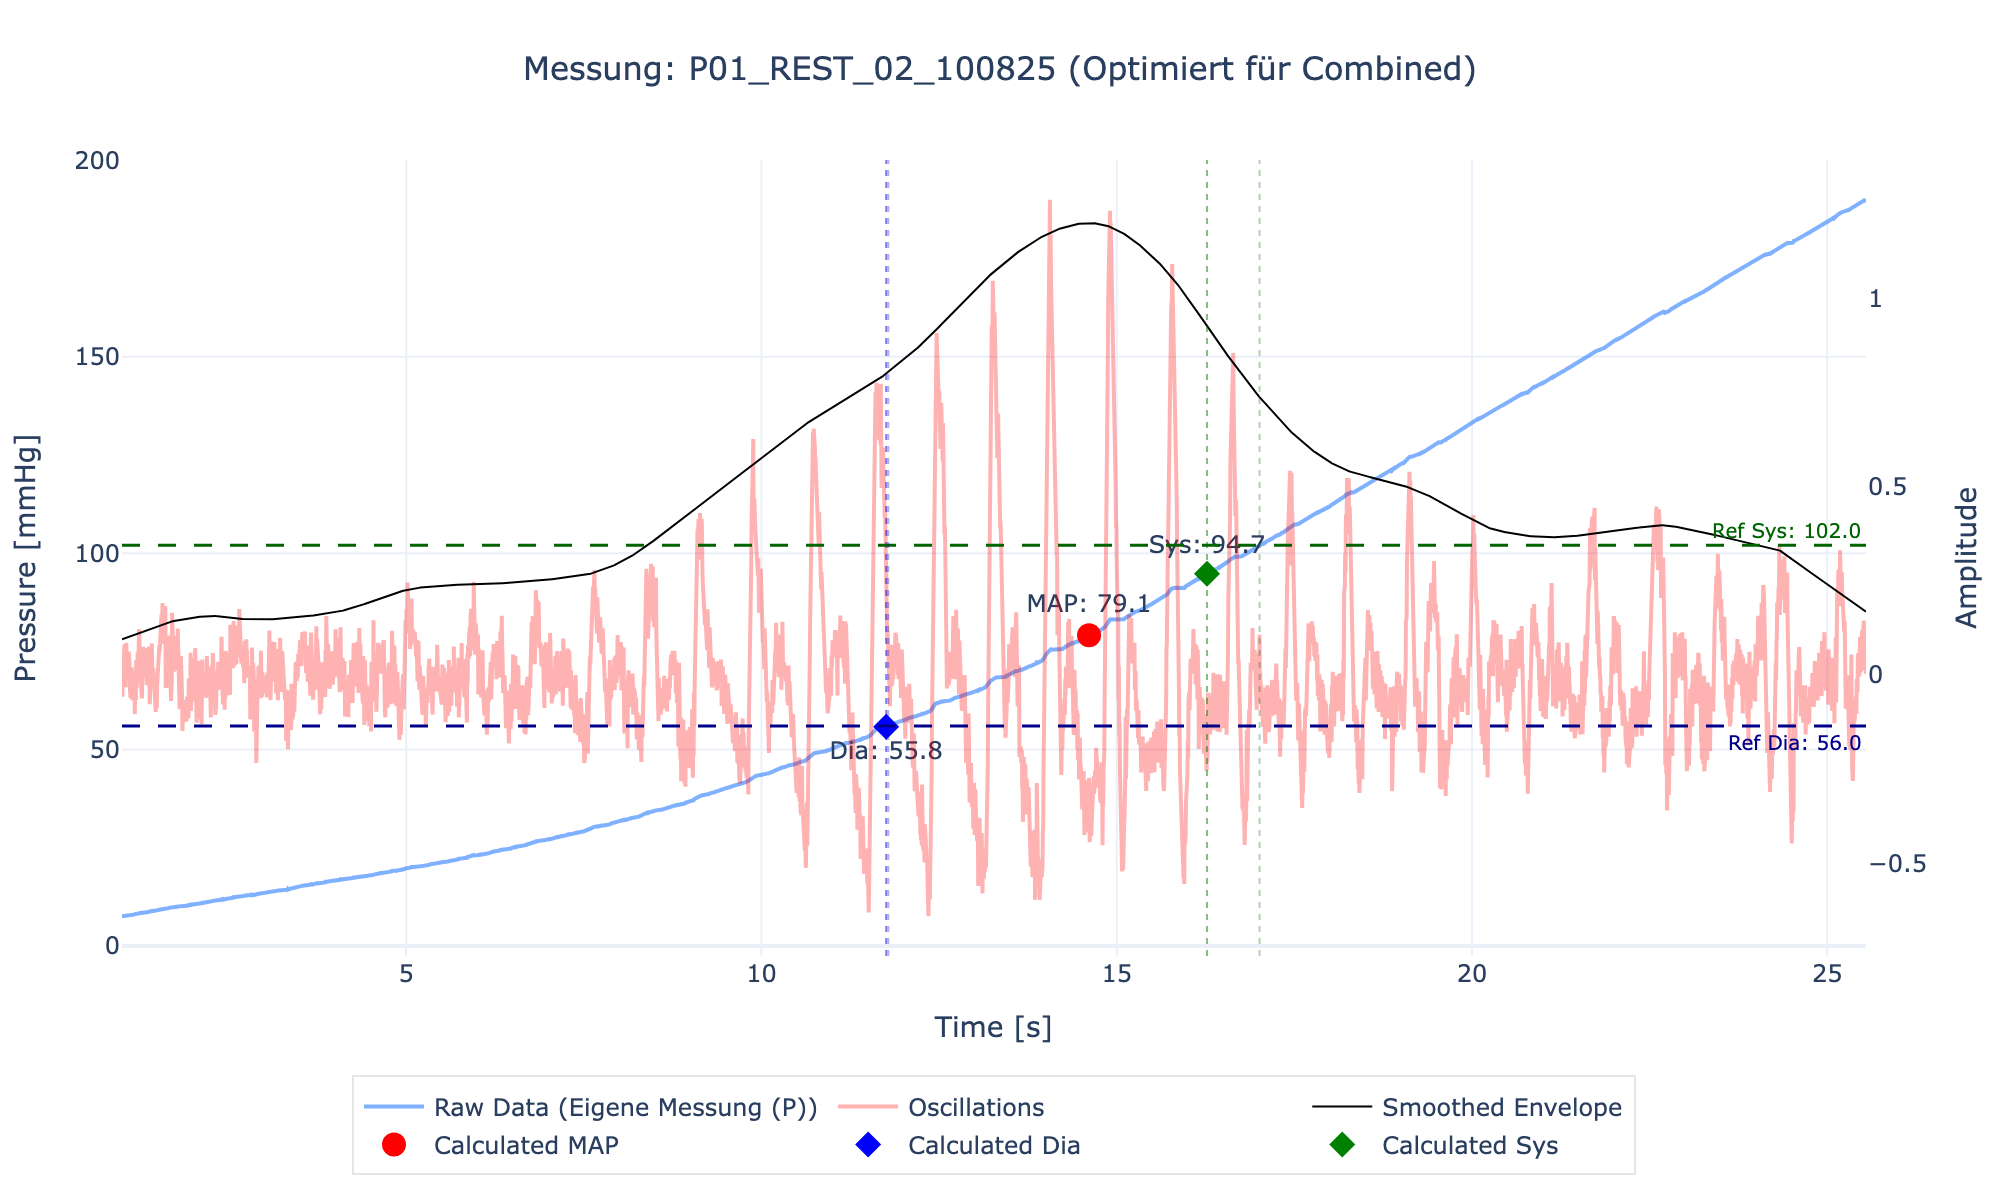
\includegraphics[width=\textwidth]{images/P01_REST_02_100825_combined.png}
        \caption{Optimiert für Beurer und NAIS (Kombiniert)}
    \end{subfigure} \\
    \begin{subfigure}[b]{0.48\textwidth}
        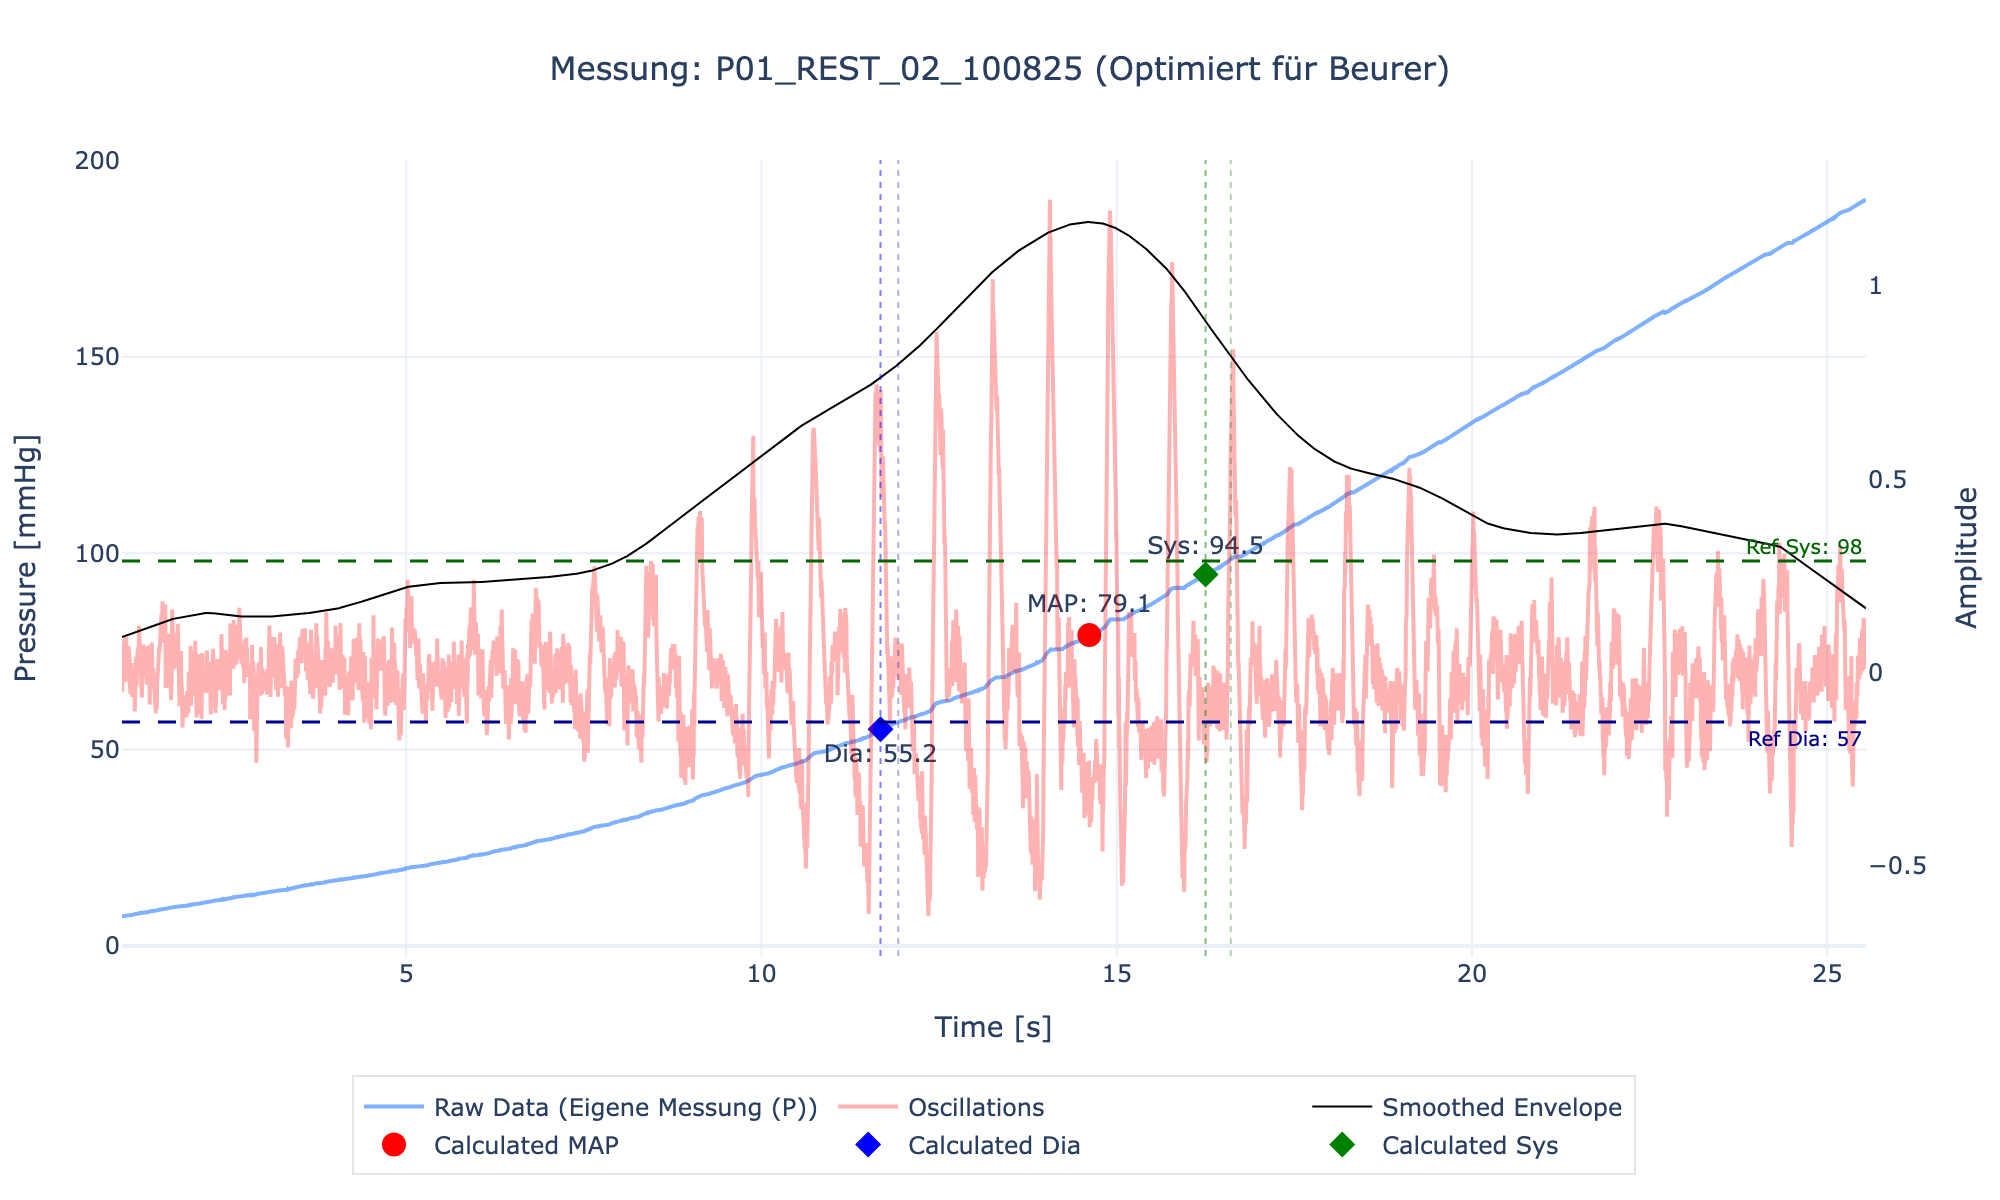
\includegraphics[width=\textwidth]{images/P01_REST_02_100825_beurer.png}
        \caption{Optimiert für Beurer}
    \end{subfigure}
    \hfill
    \begin{subfigure}[b]{0.48\textwidth}
        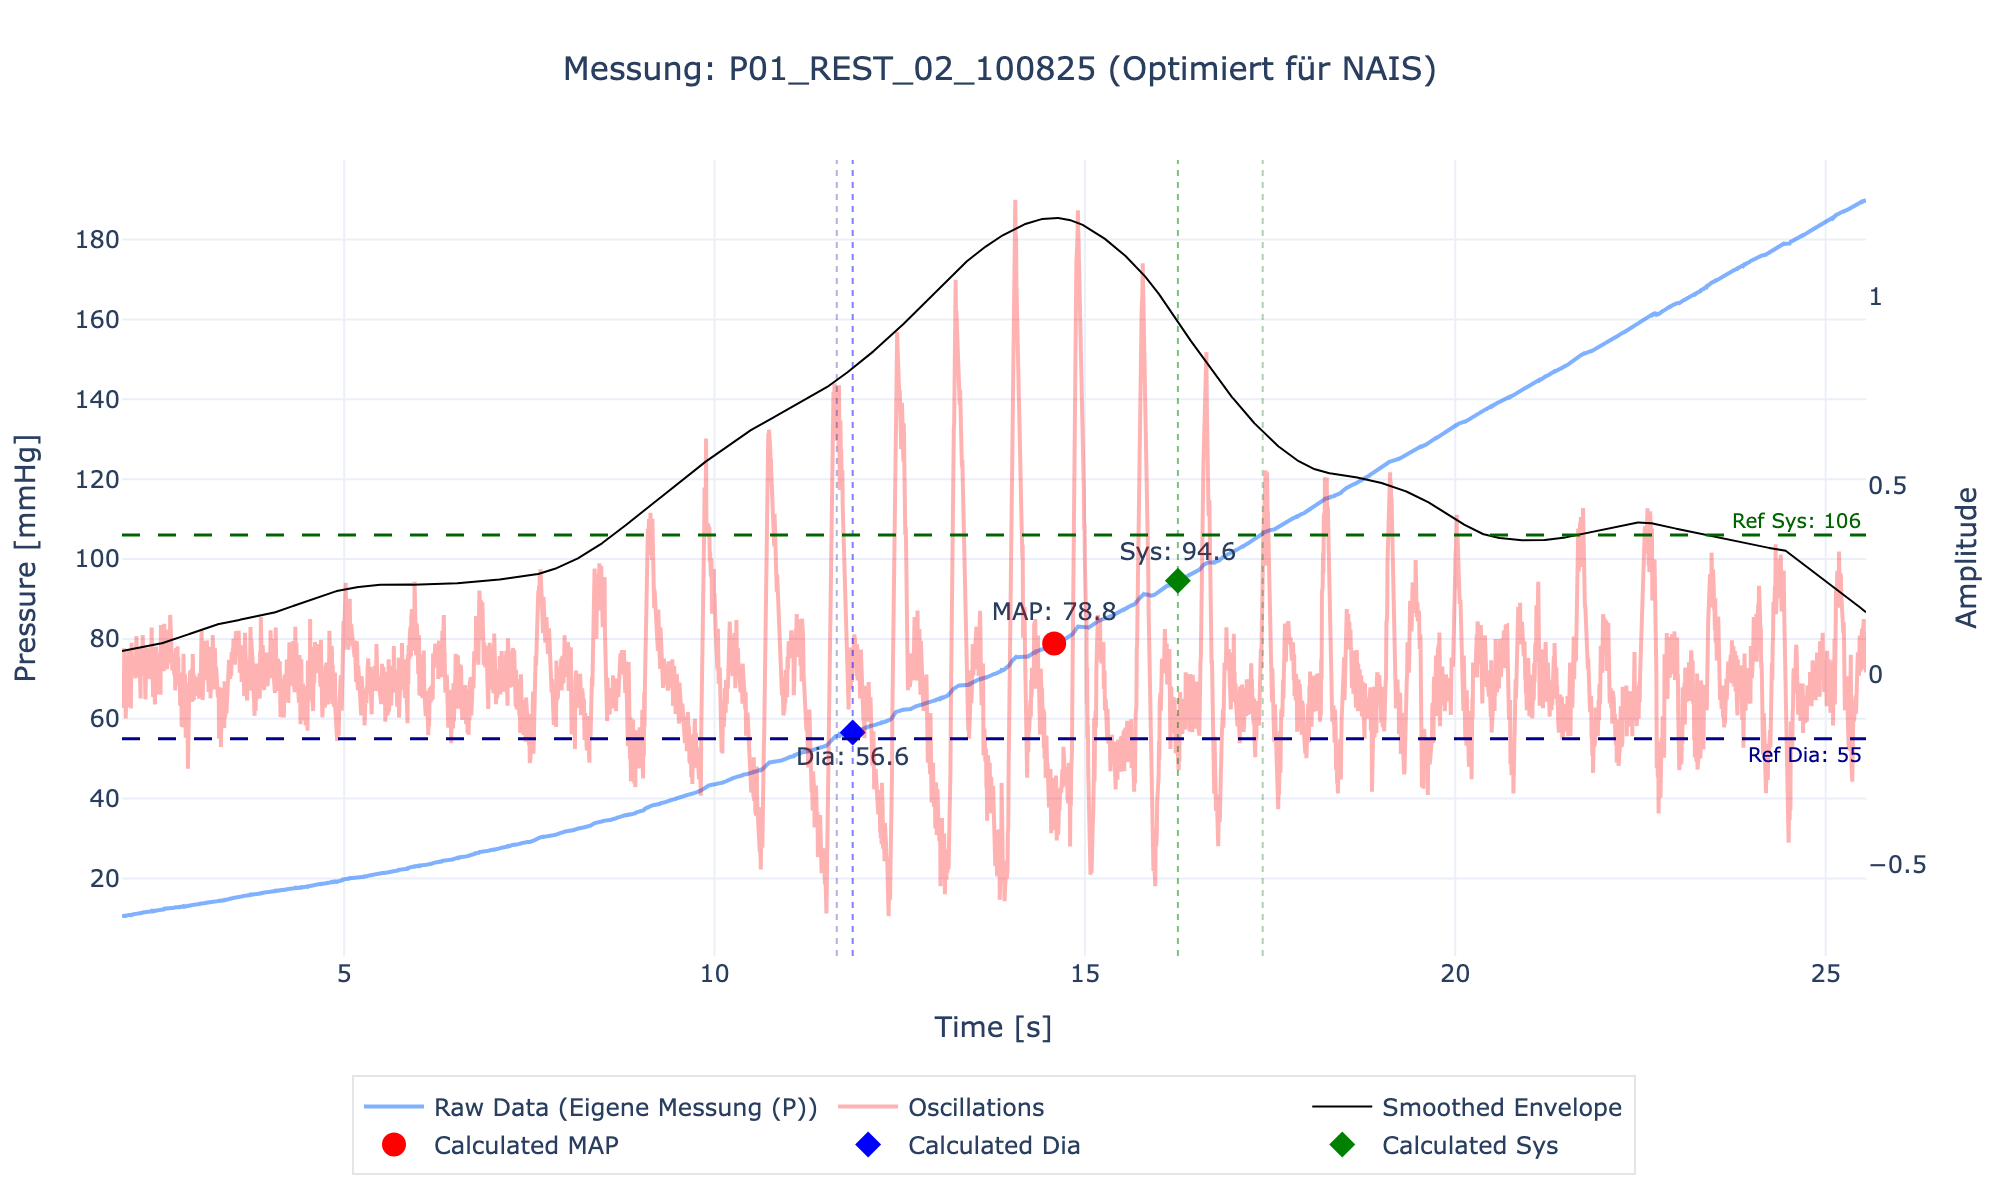
\includegraphics[width=\textwidth]{images/P01_REST_02_100825_nais.png}
        \caption{Optimiert für NAIS}
    \end{subfigure}
    \caption{Einzelauswertung der Messung P01\_REST\_02\_100825 mit verschiedenen Parametersätzen.}
\end{figure}
\newpage

\subsection*{Messung: P02\_ACTIV\_01\_160925}
\begin{figure}[H]
    \centering
    \begin{subfigure}[b]{0.8\textwidth}
        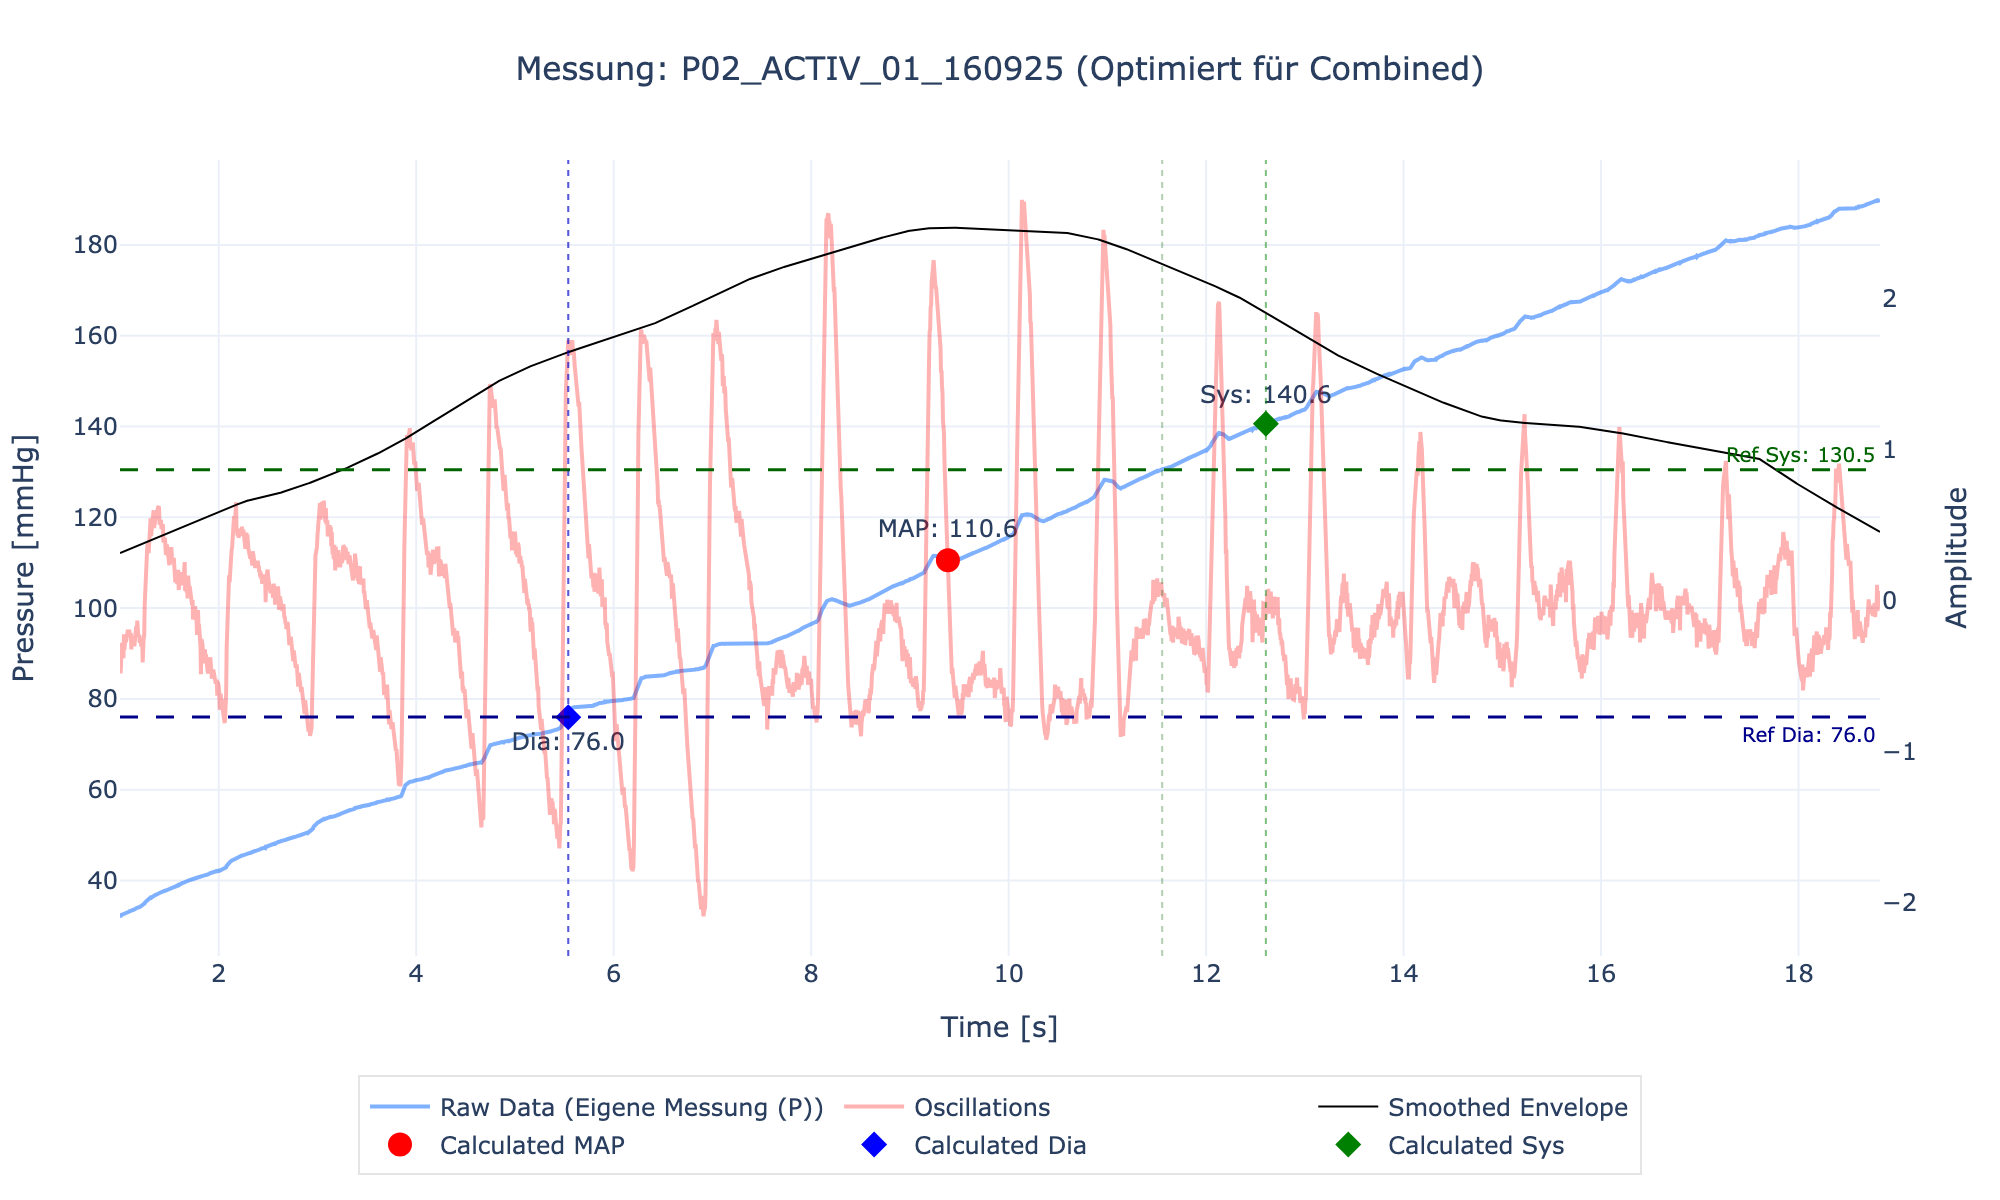
\includegraphics[width=\textwidth]{images/P02_ACTIV_01_160925_combined.png}
        \caption{Optimiert für Beurer und NAIS (Kombiniert)}
    \end{subfigure} \\
    \begin{subfigure}[b]{0.48\textwidth}
        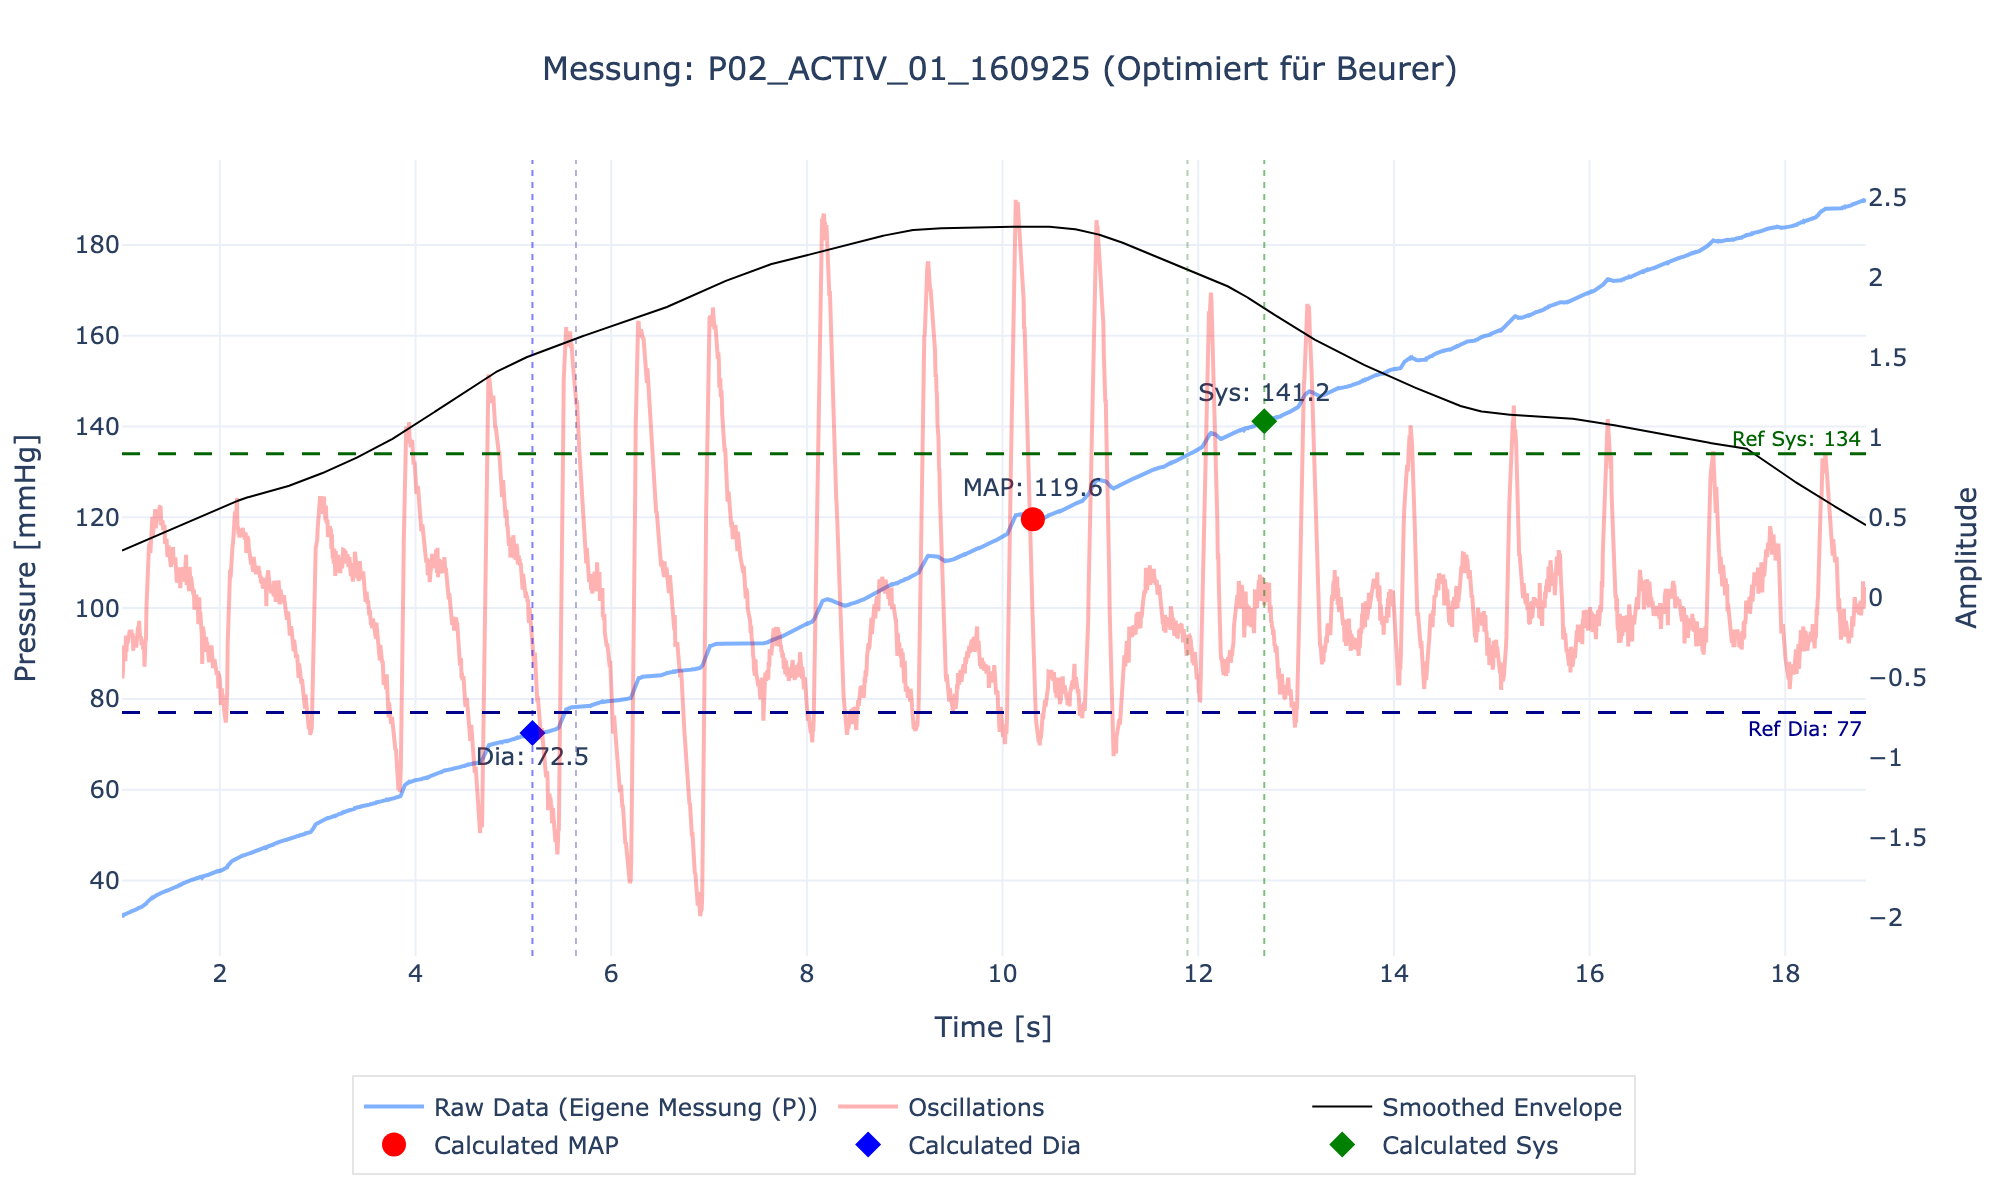
\includegraphics[width=\textwidth]{images/P02_ACTIV_01_160925_beurer.png}
        \caption{Optimiert für Beurer}
    \end{subfigure}
    \hfill
    \begin{subfigure}[b]{0.48\textwidth}
        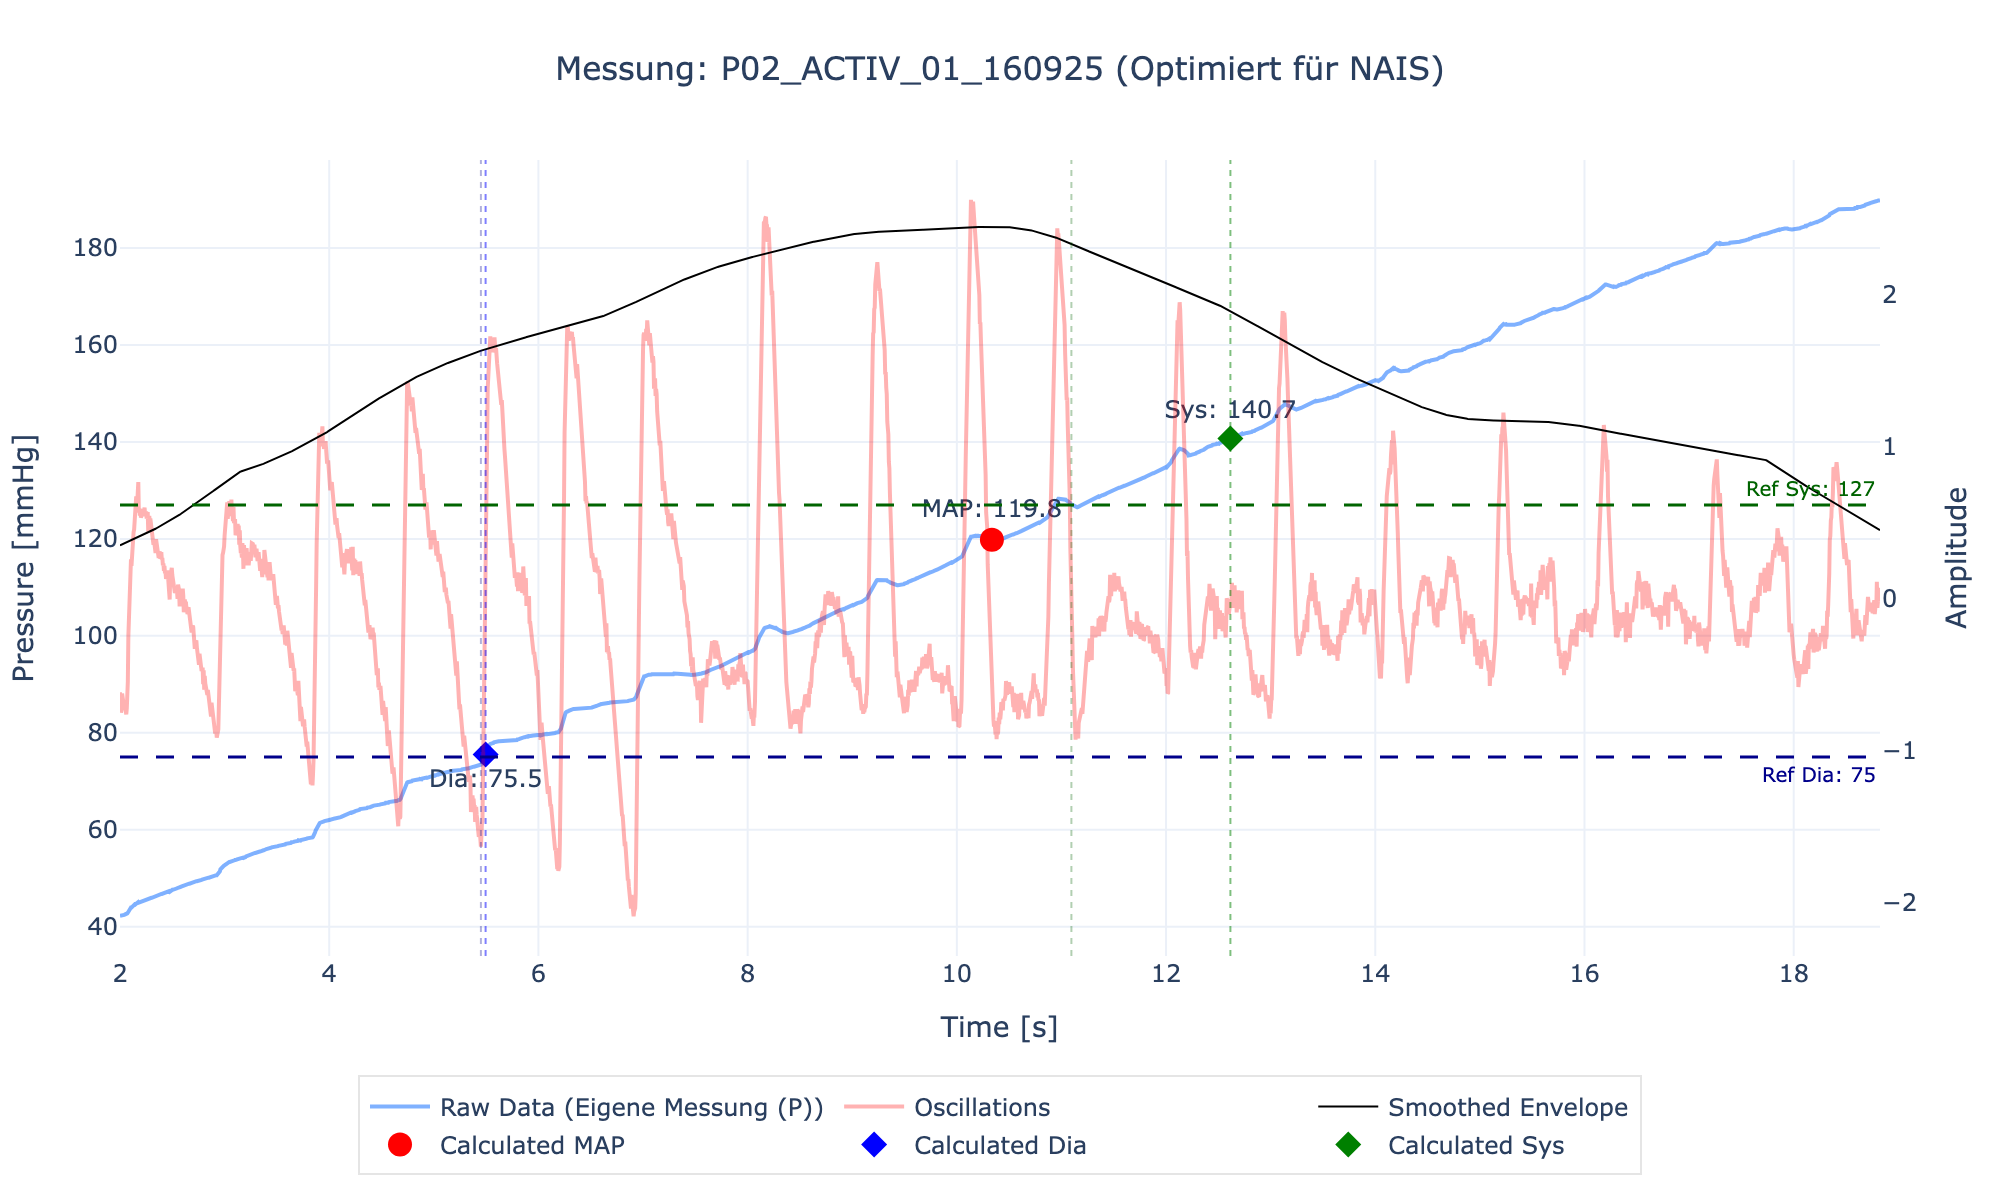
\includegraphics[width=\textwidth]{images/P02_ACTIV_01_160925_nais.png}
        \caption{Optimiert für NAIS}
    \end{subfigure}
    \caption{Einzelauswertung der Messung P02\_ACTIV\_01\_160925 mit verschiedenen Parametersätzen.}
\end{figure}
\newpage

\subsection*{Messung: P02\_REST\_01\_100825}
\begin{figure}[H]
    \centering
    \begin{subfigure}[b]{0.8\textwidth}
        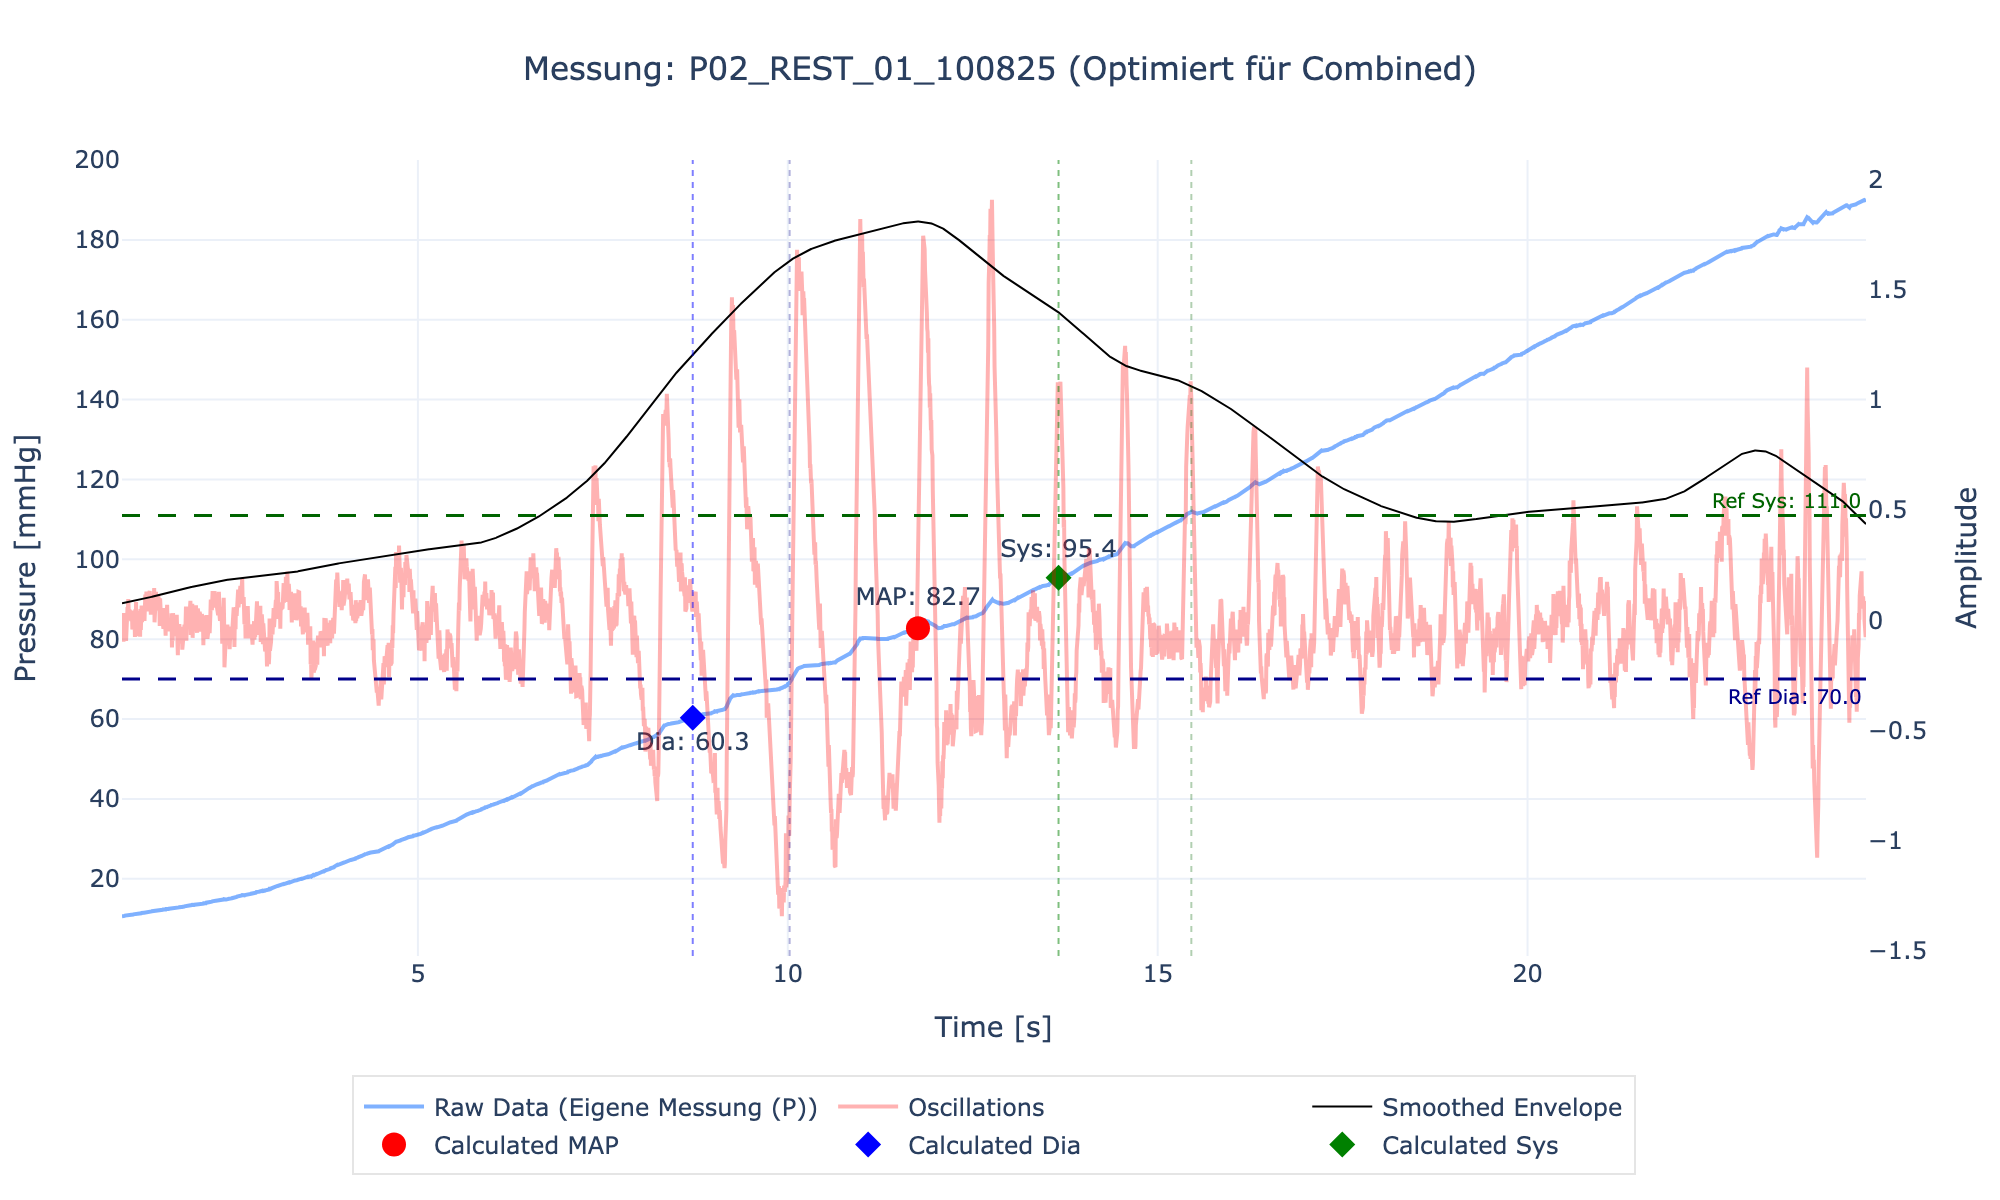
\includegraphics[width=\textwidth]{images/P02_REST_01_100825_combined.png}
        \caption{Optimiert für Beurer und NAIS (Kombiniert)}
    \end{subfigure} \\
    \begin{subfigure}[b]{0.48\textwidth}
        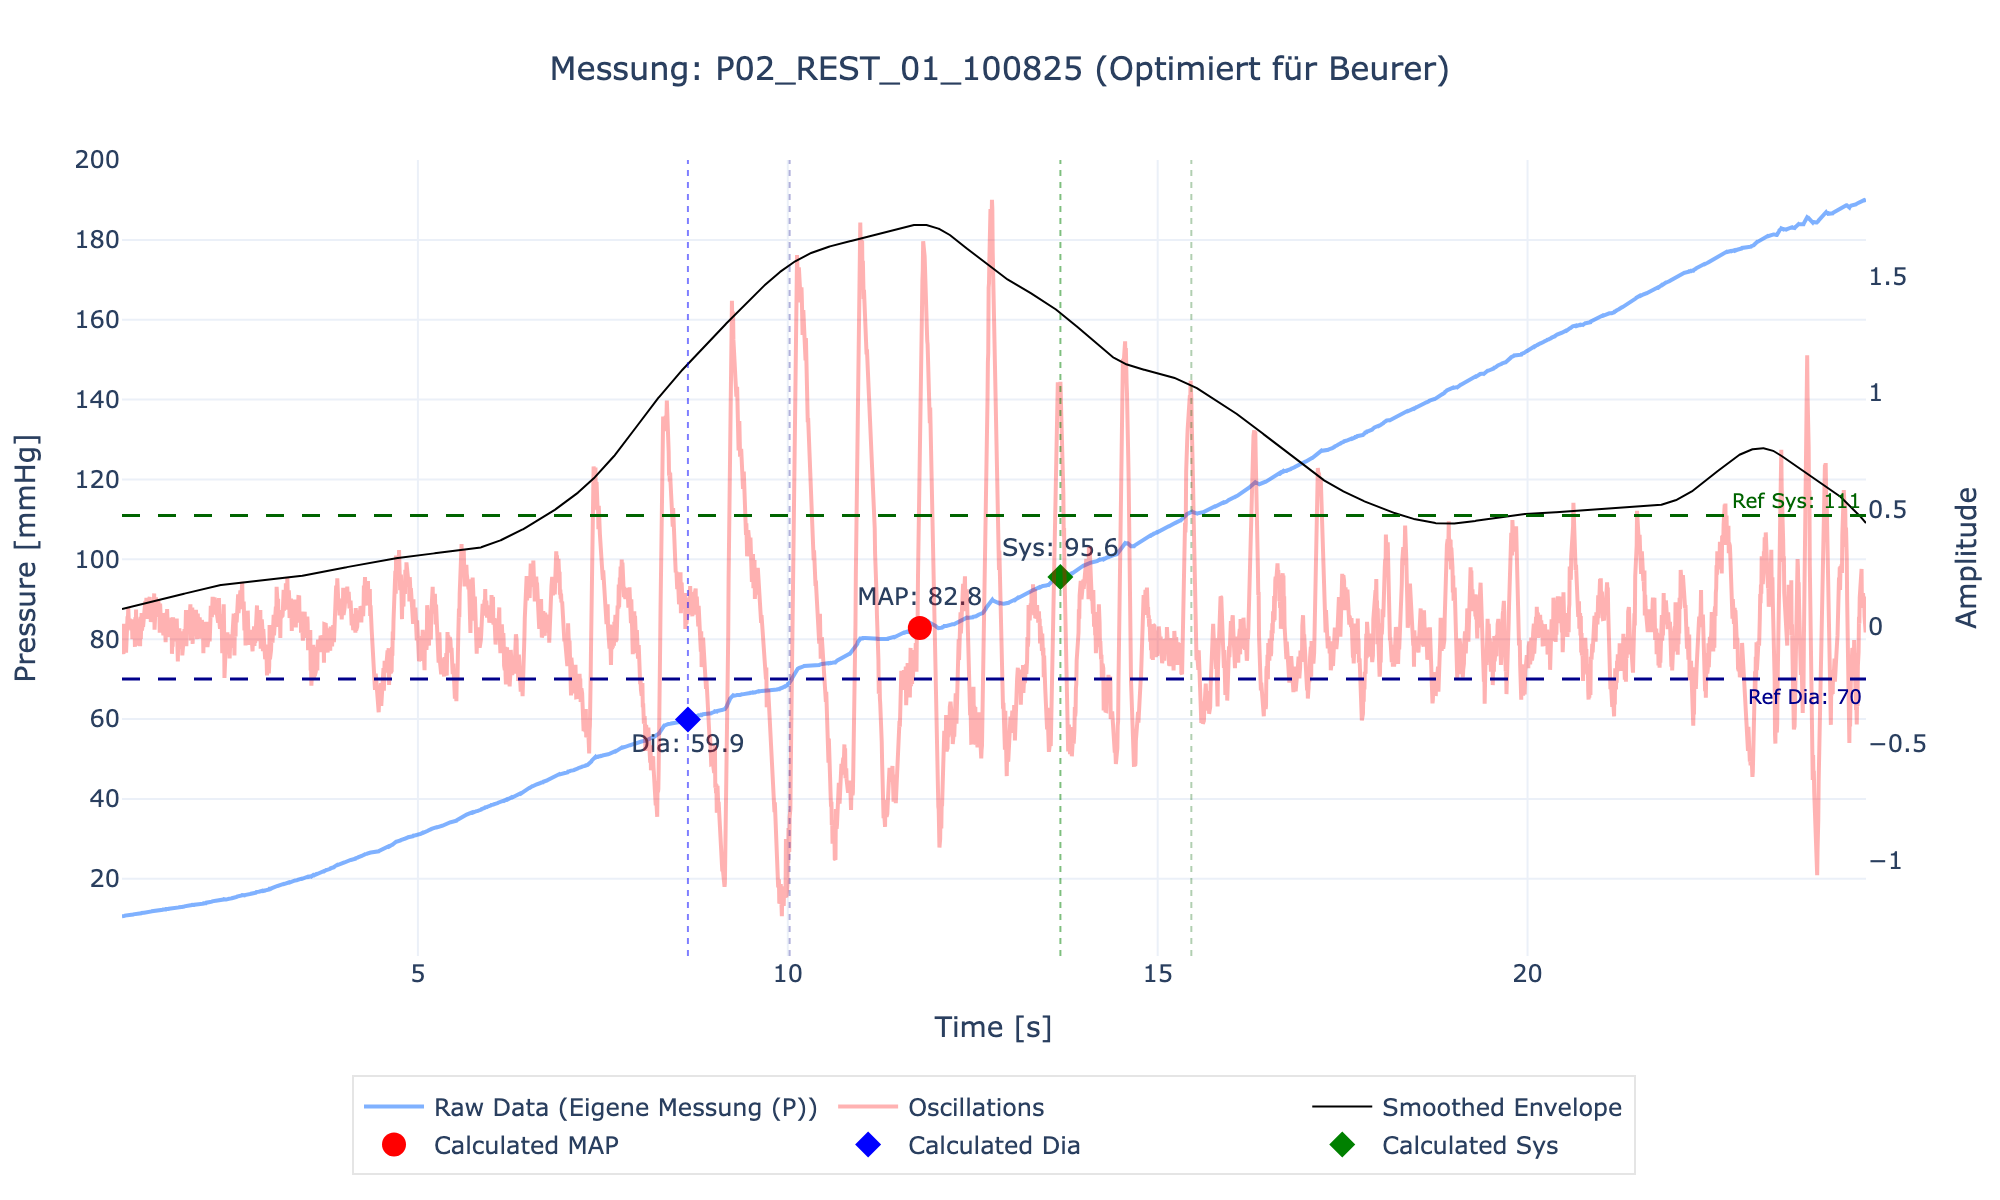
\includegraphics[width=\textwidth]{images/P02_REST_01_100825_beurer.png}
        \caption{Optimiert für Beurer}
    \end{subfigure}
    \hfill
    \begin{subfigure}[b]{0.48\textwidth}
        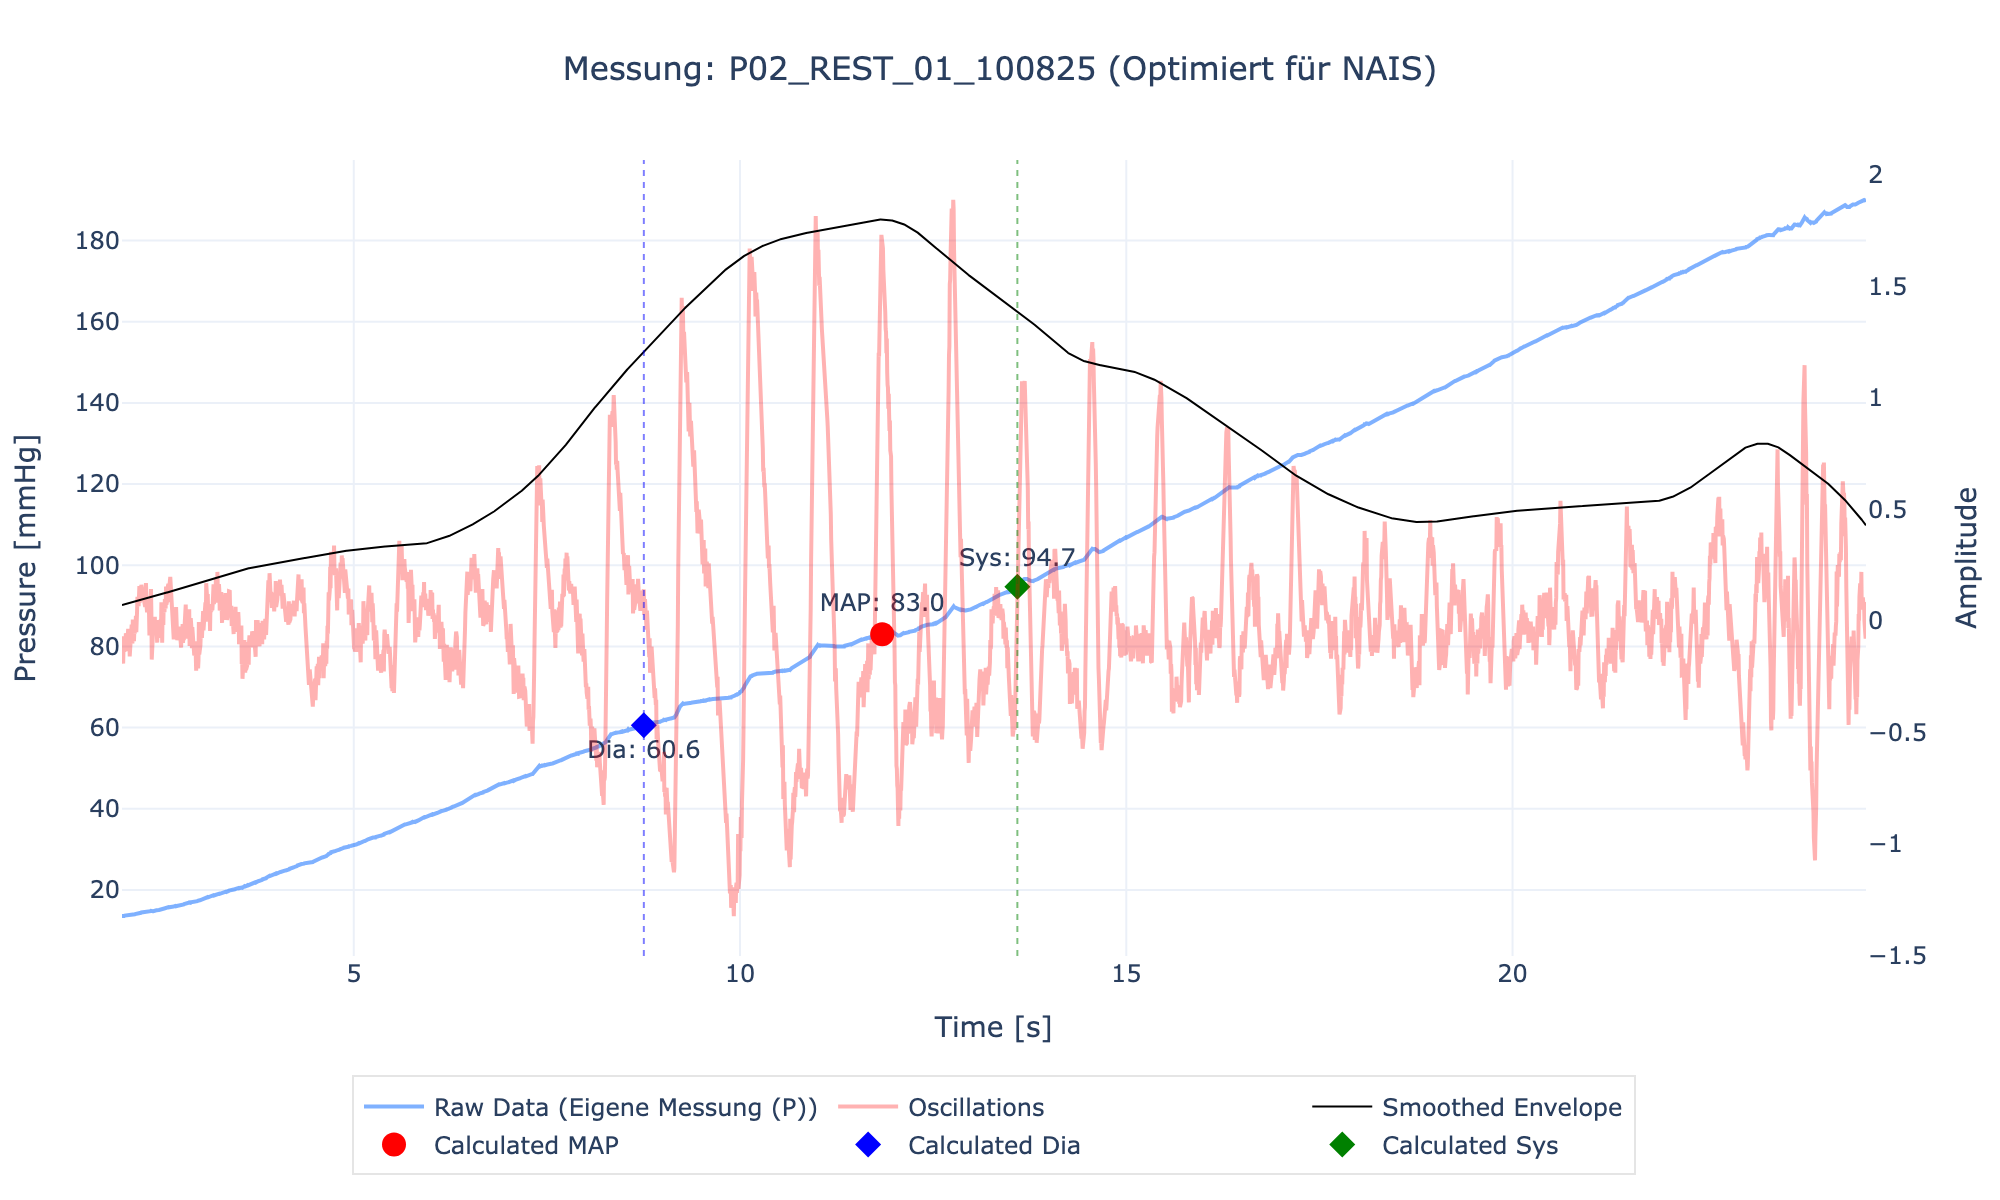
\includegraphics[width=\textwidth]{images/P02_REST_01_100825_nais.png}
        \caption{Optimiert für NAIS}
    \end{subfigure}
    \caption{Einzelauswertung der Messung P02\_REST\_01\_100825 mit verschiedenen Parametersätzen.}
\end{figure}
\newpage

\subsection*{Messung: P02\_REST\_02\_160925}
\begin{figure}[H]
    \centering
    \begin{subfigure}[b]{0.8\textwidth}
        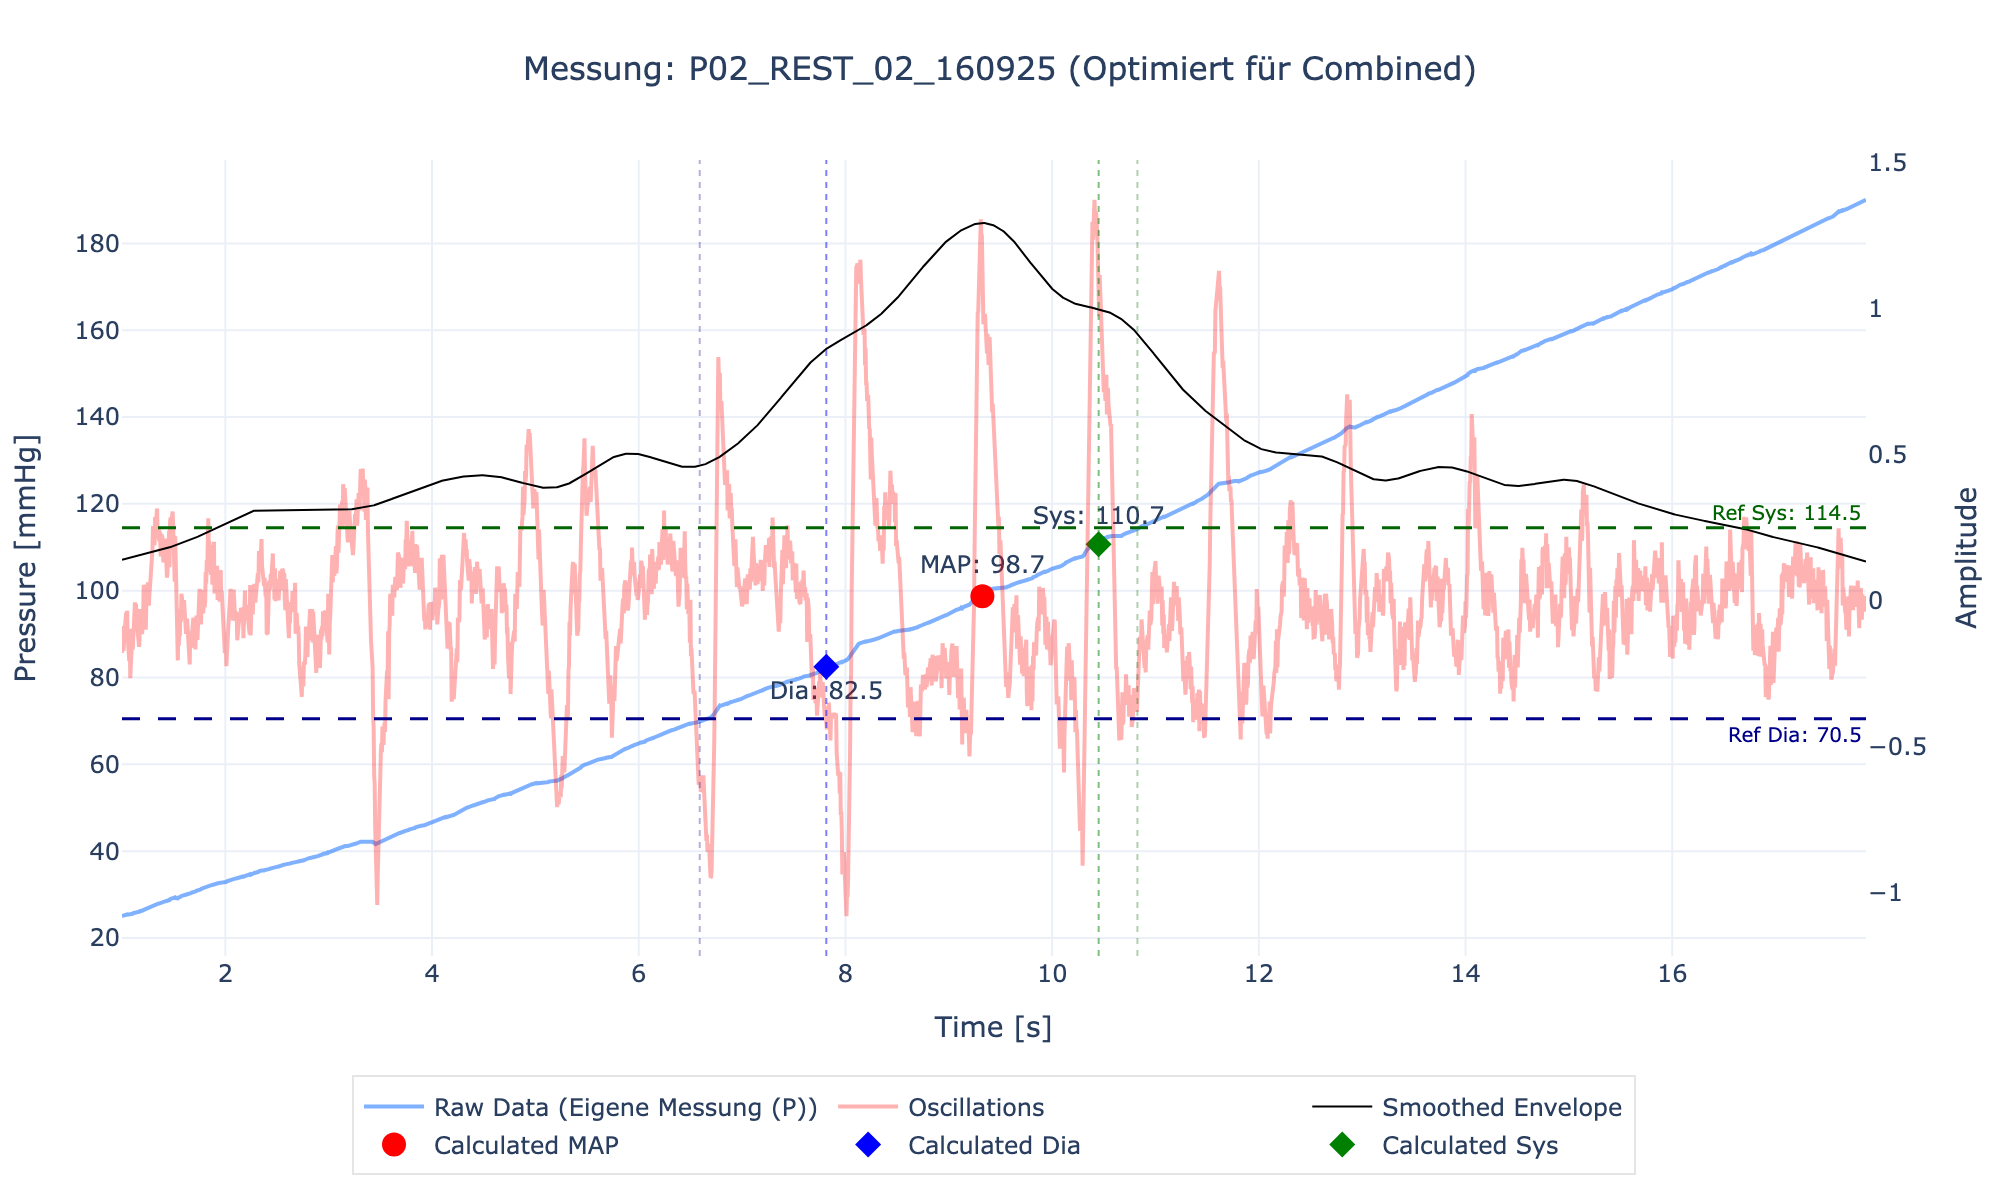
\includegraphics[width=\textwidth]{images/P02_REST_02_160925_combined.png}
        \caption{Optimiert für Beurer und NAIS (Kombiniert)}
    \end{subfigure} \\
    \begin{subfigure}[b]{0.48\textwidth}
        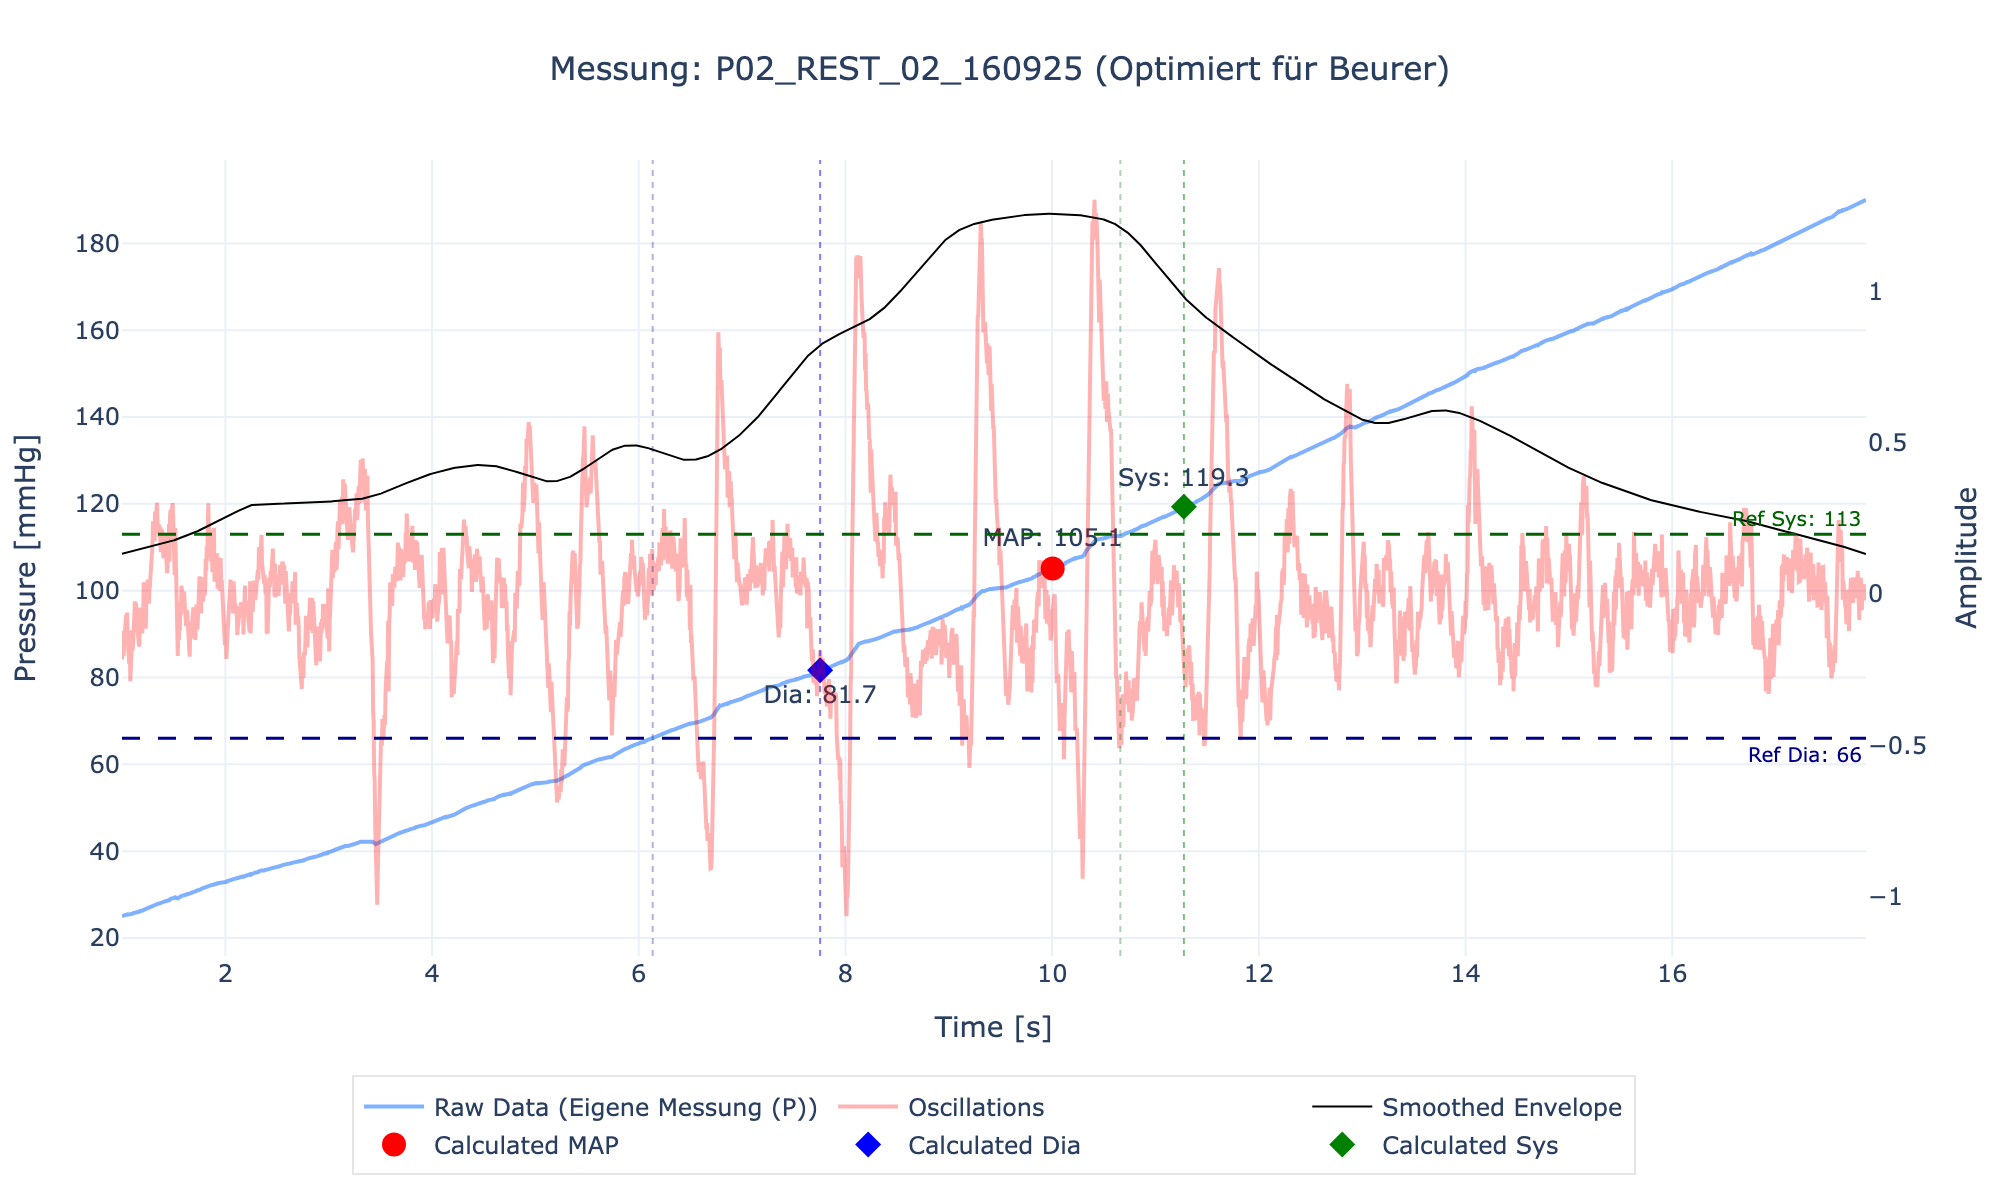
\includegraphics[width=\textwidth]{images/P02_REST_02_160925_beurer.png}
        \caption{Optimiert für Beurer}
    \end{subfigure}
    \hfill
    \begin{subfigure}[b]{0.48\textwidth}
        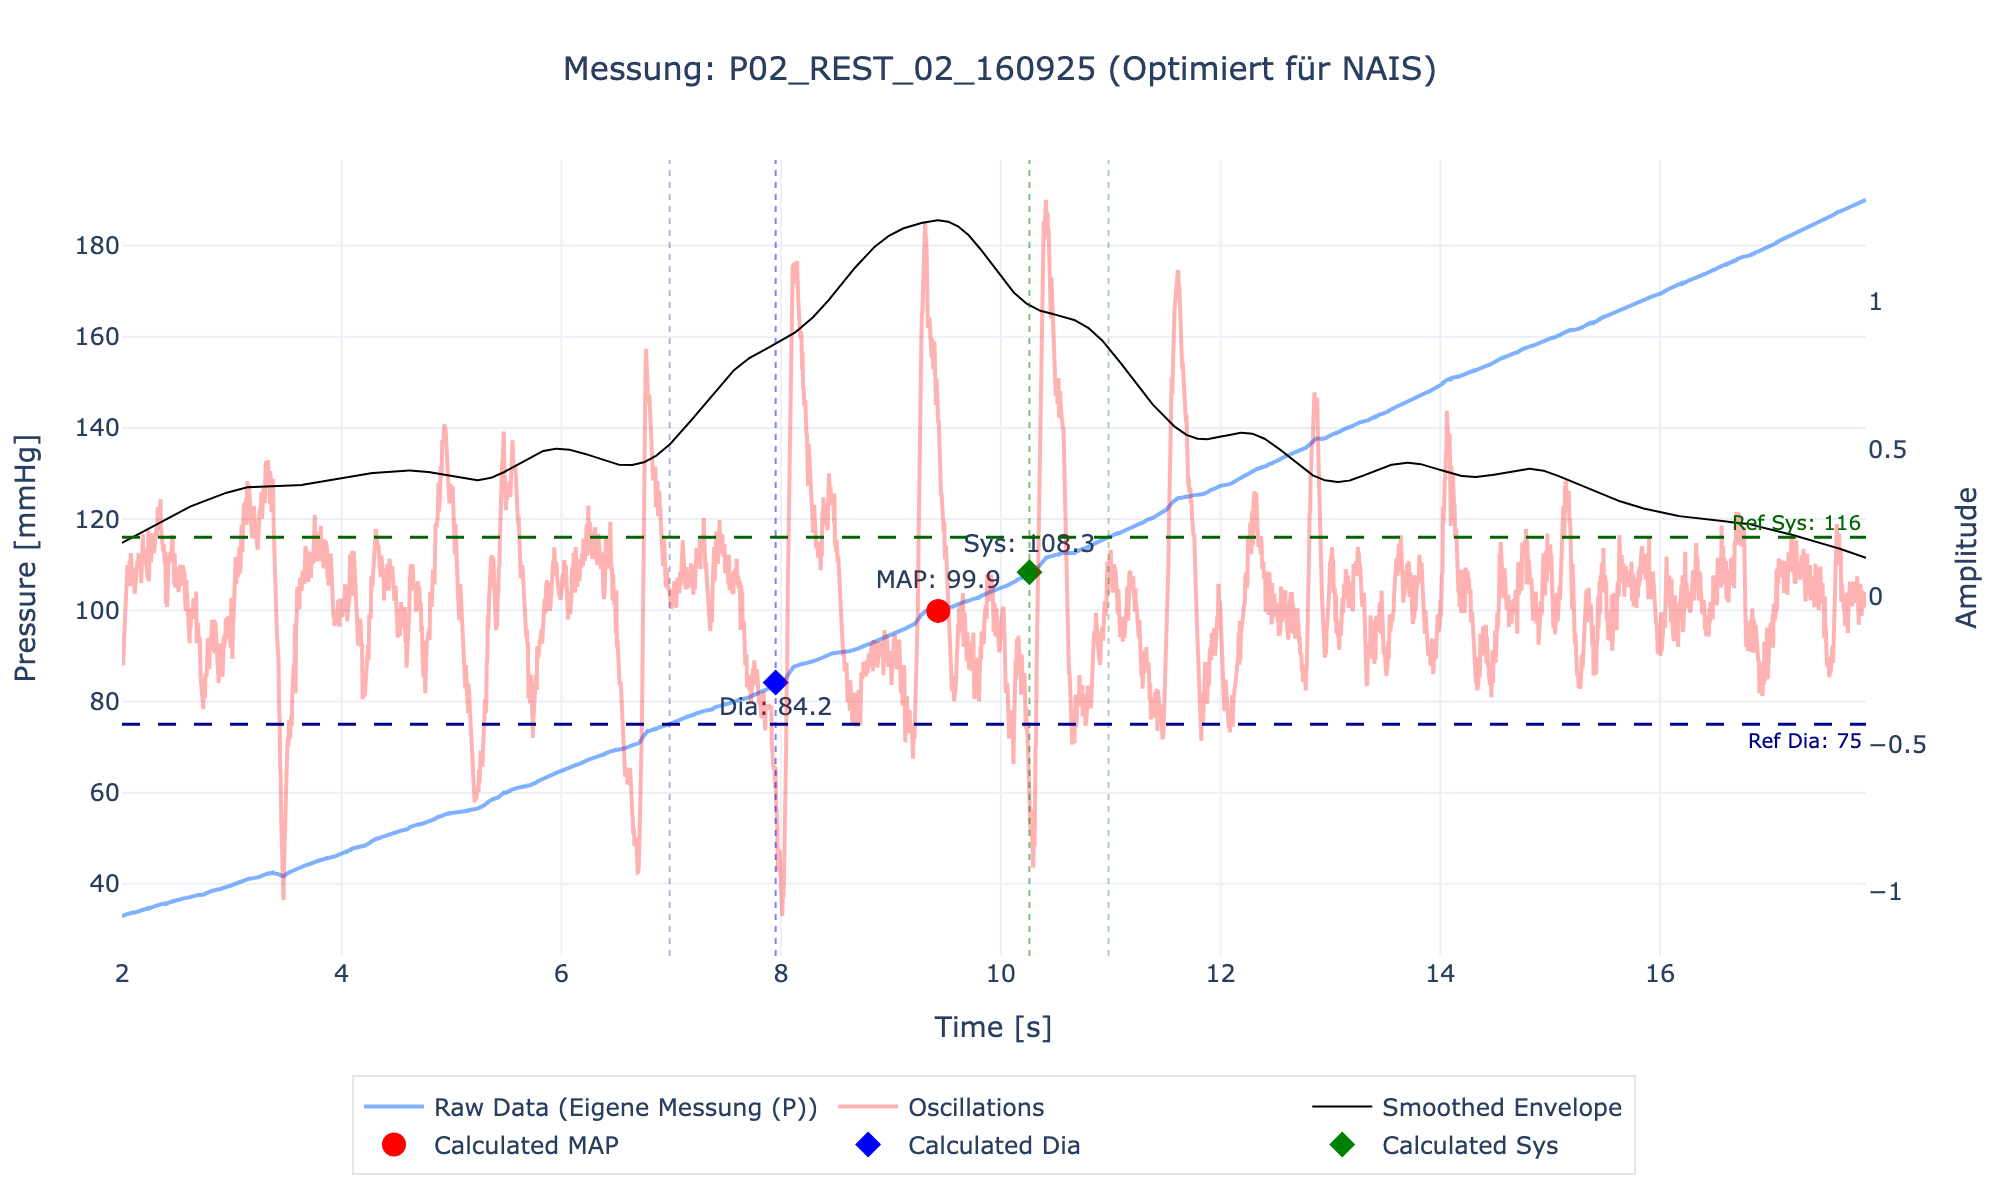
\includegraphics[width=\textwidth]{images/P02_REST_02_160925_nais.png}
        \caption{Optimiert für NAIS}
    \end{subfigure}
    \caption{Einzelauswertung der Messung P02\_REST\_02\_160925 mit verschiedenen Parametersätzen.}
\end{figure}
\newpage

\subsection*{Messung: P03\_ACTIV\_02\_160925}
\begin{figure}[H]
    \centering
    \begin{subfigure}[b]{0.8\textwidth}
        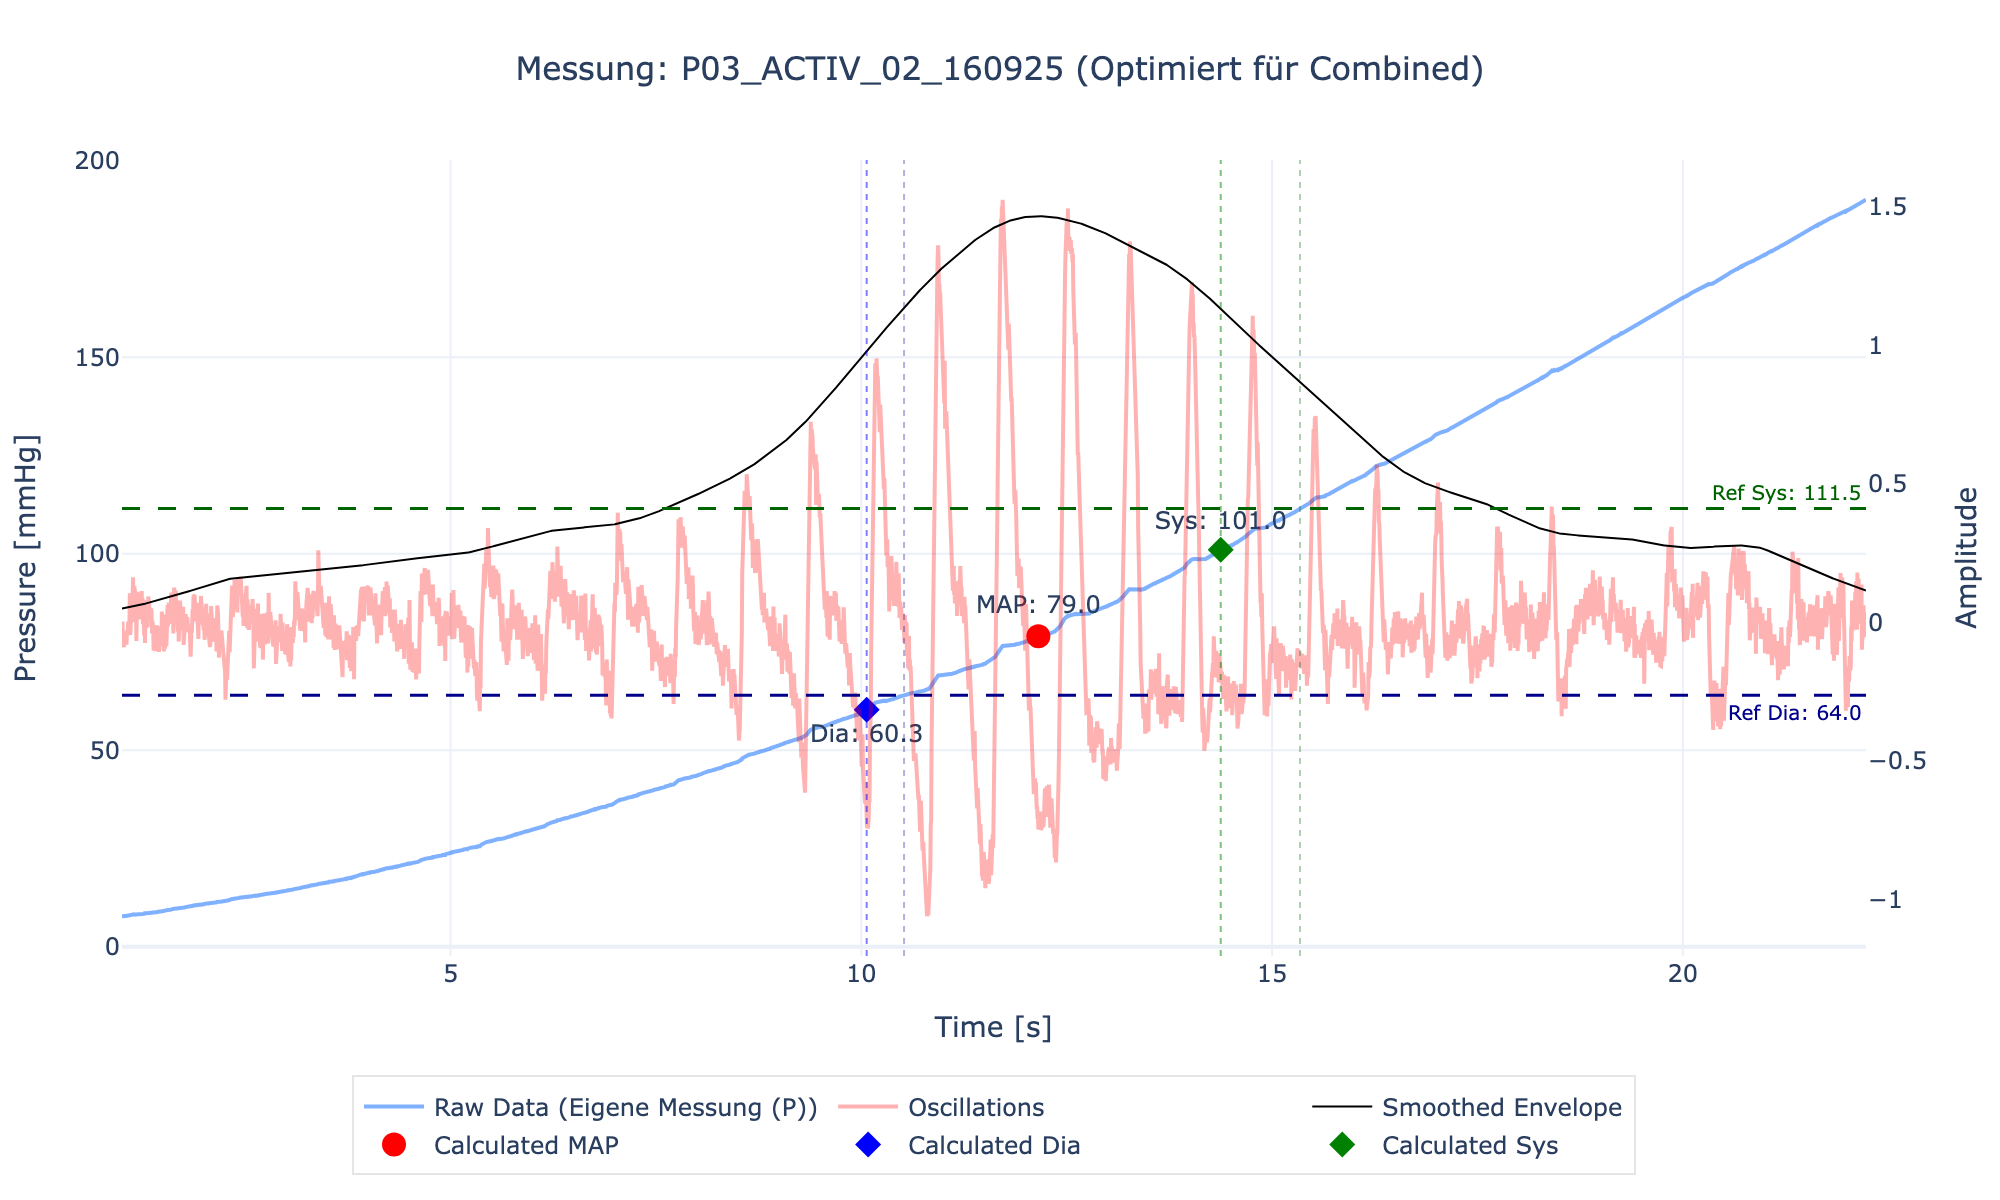
\includegraphics[width=\textwidth]{images/P03_ACTIV_02_160925_combined.png}
        \caption{Optimiert für Beurer und NAIS (Kombiniert)}
    \end{subfigure} \\
    \begin{subfigure}[b]{0.48\textwidth}
        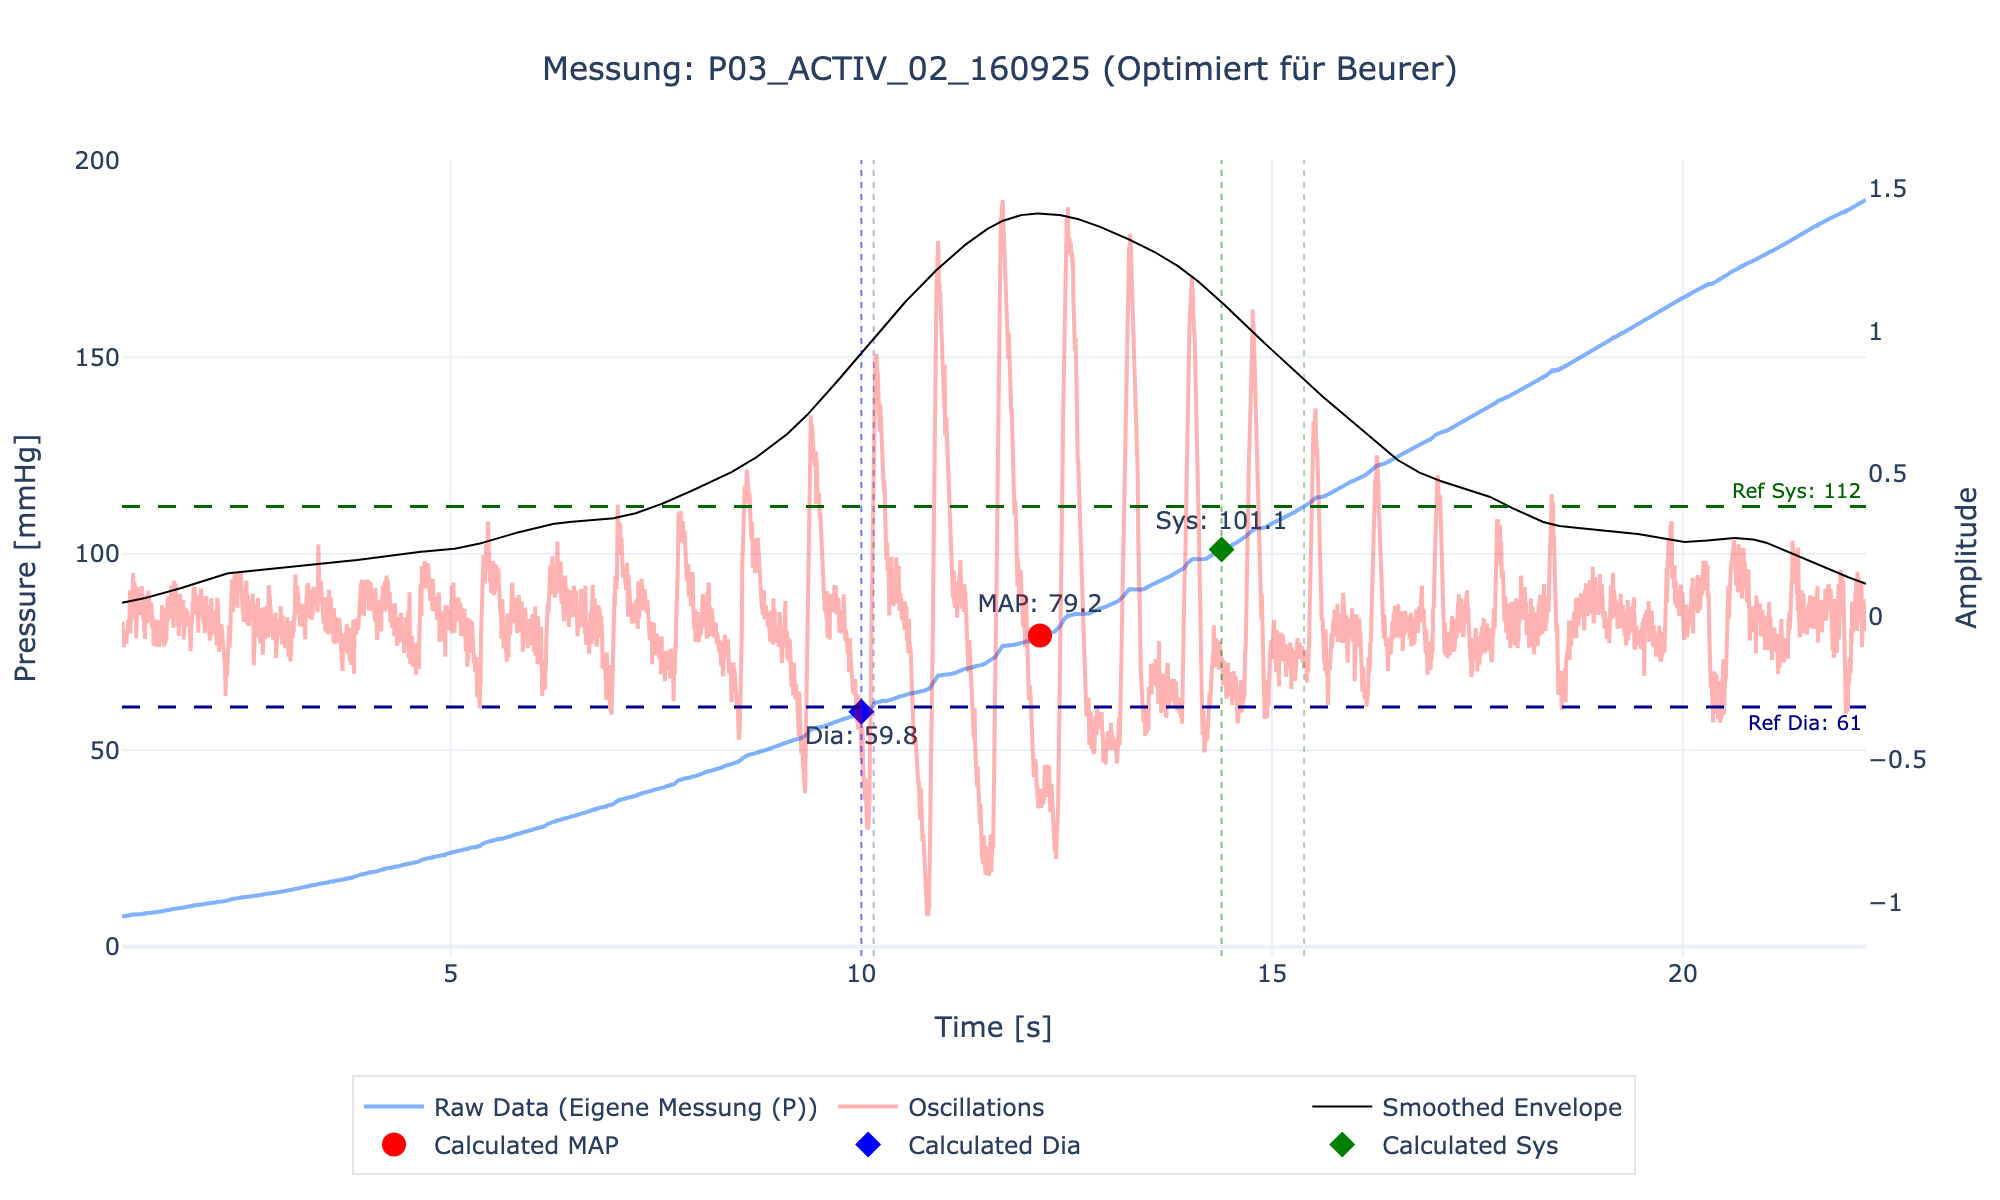
\includegraphics[width=\textwidth]{images/P03_ACTIV_02_160925_beurer.png}
        \caption{Optimiert für Beurer}
    \end{subfigure}
    \hfill
    \begin{subfigure}[b]{0.48\textwidth}
        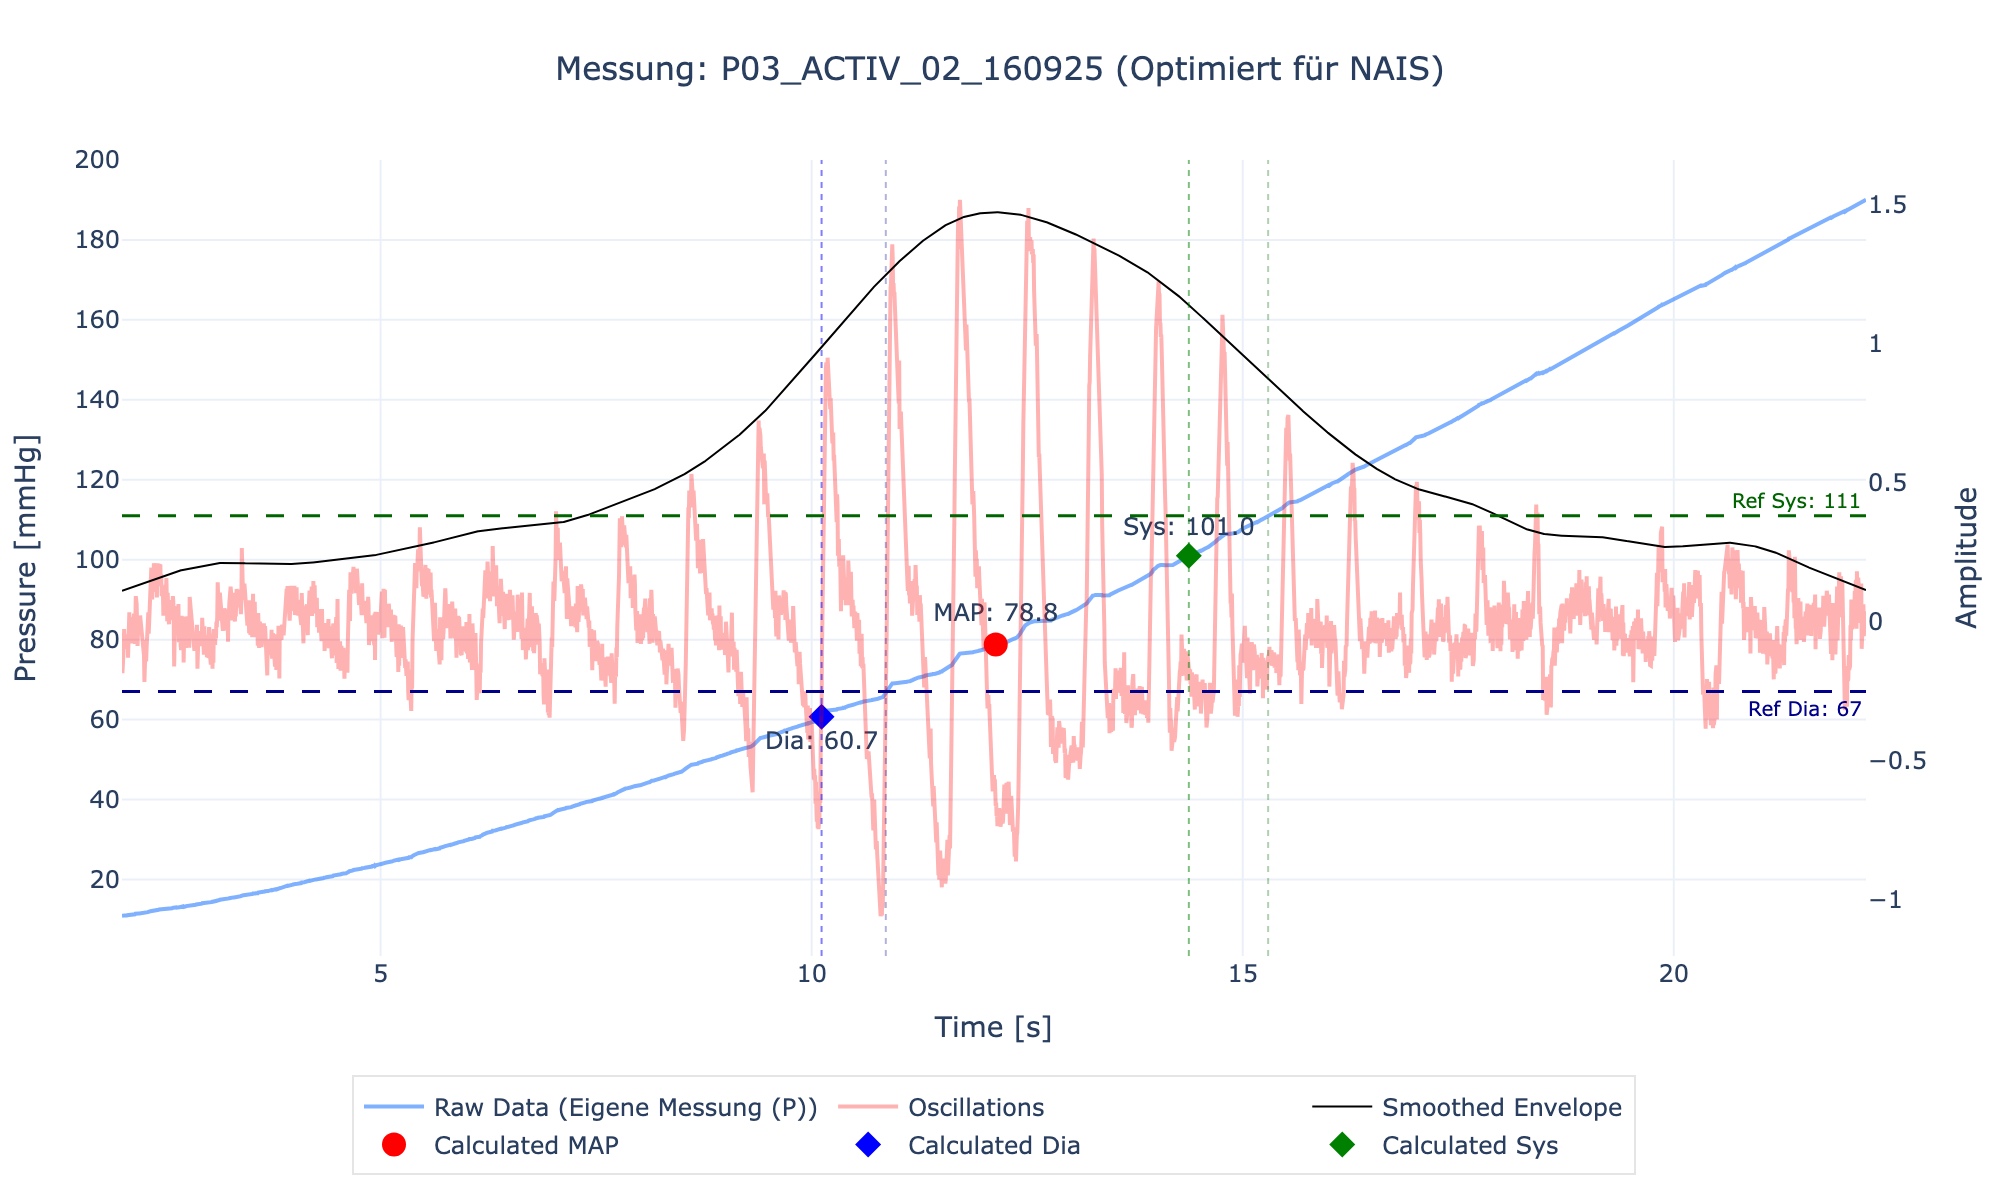
\includegraphics[width=\textwidth]{images/P03_ACTIV_02_160925_nais.png}
        \caption{Optimiert für NAIS}
    \end{subfigure}
    \caption{Einzelauswertung der Messung P03\_ACTIV\_02\_160925 mit verschiedenen Parametersätzen.}
\end{figure}
\newpage

\subsection*{Messung: P03\_REST\_01\_100825}
\begin{figure}[H]
    \centering
    \begin{subfigure}[b]{0.8\textwidth}
        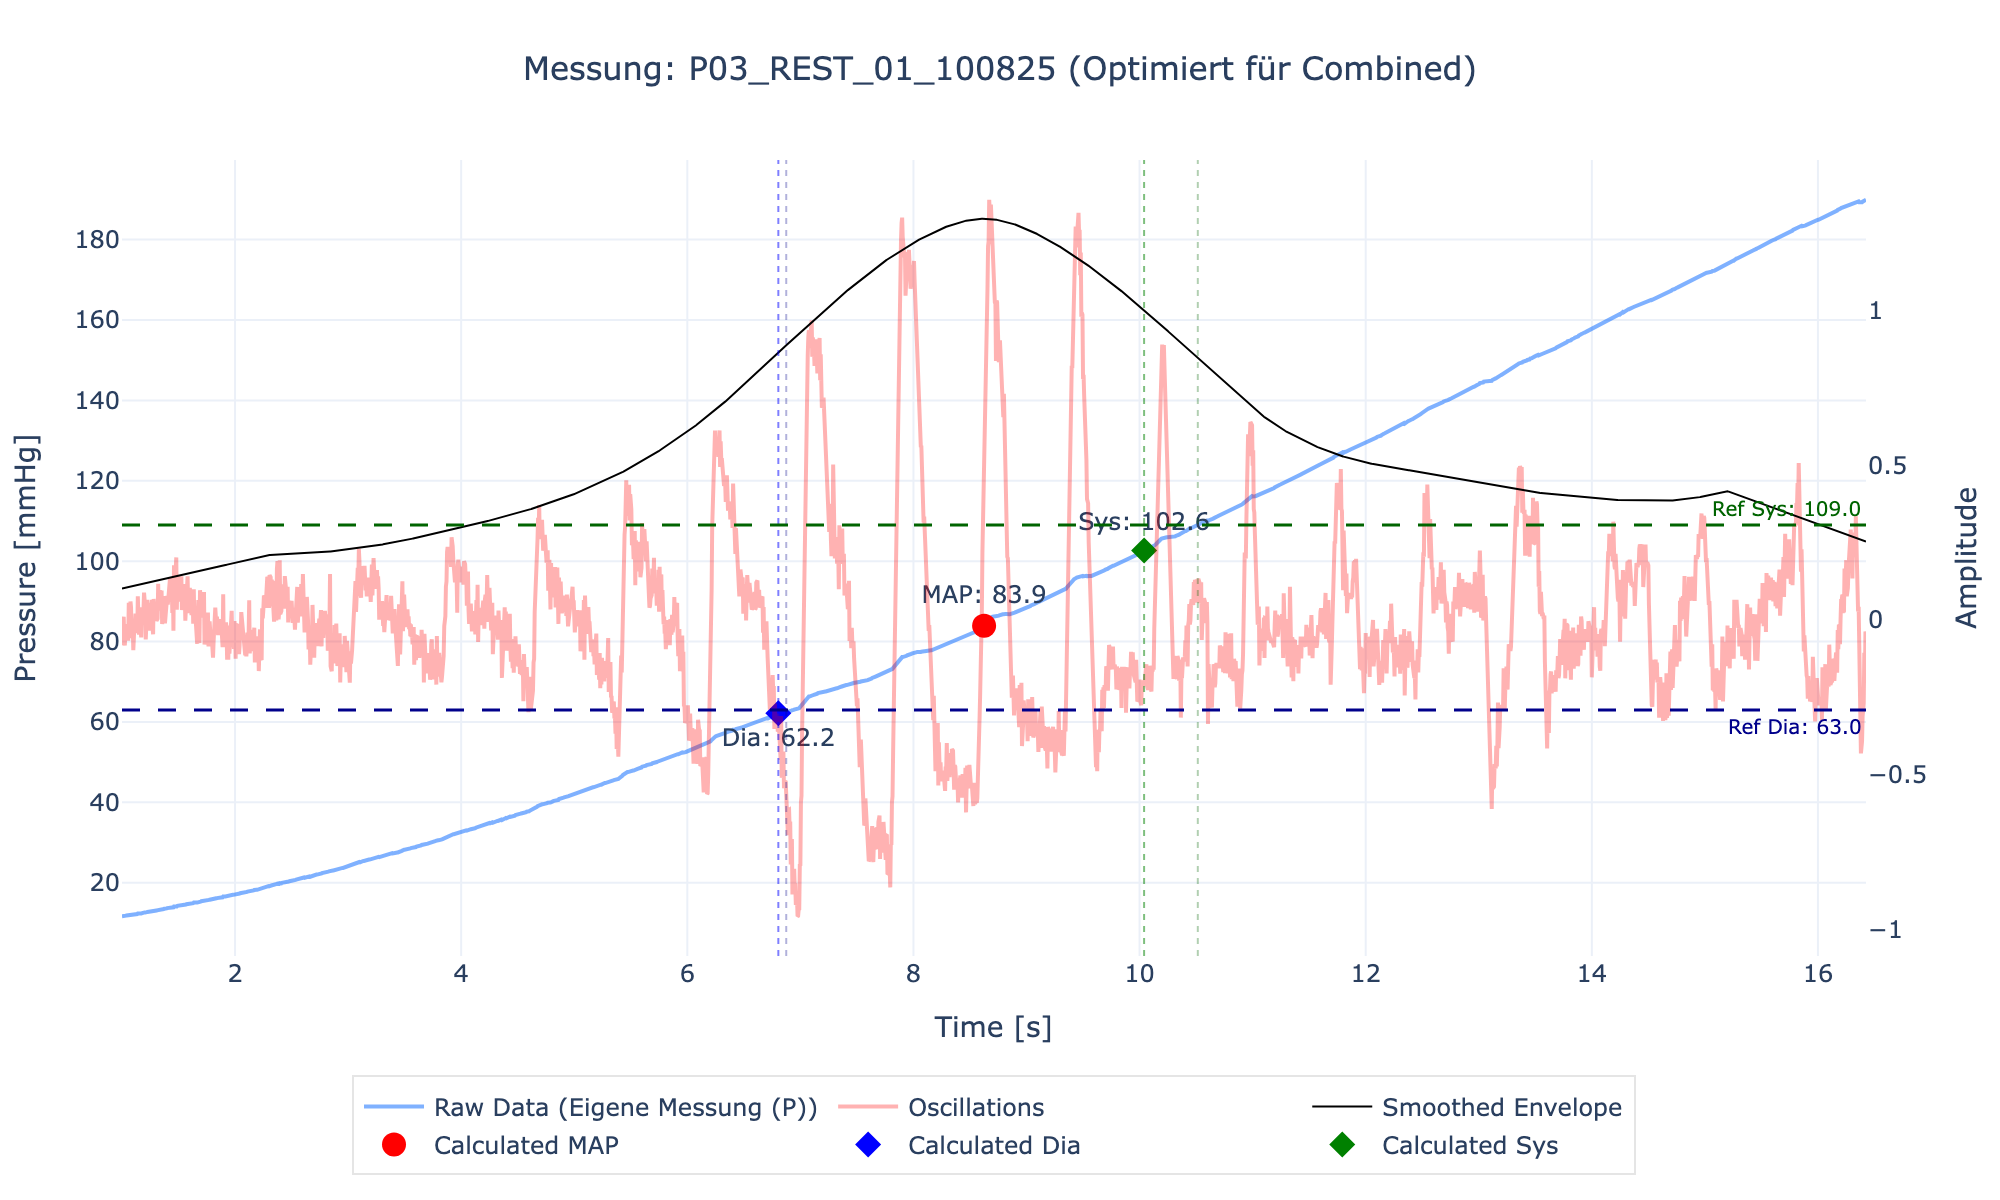
\includegraphics[width=\textwidth]{images/P03_REST_01_100825_combined.png}
        \caption{Optimiert für Beurer und NAIS (Kombiniert)}
    \end{subfigure} \\
    \begin{subfigure}[b]{0.48\textwidth}
        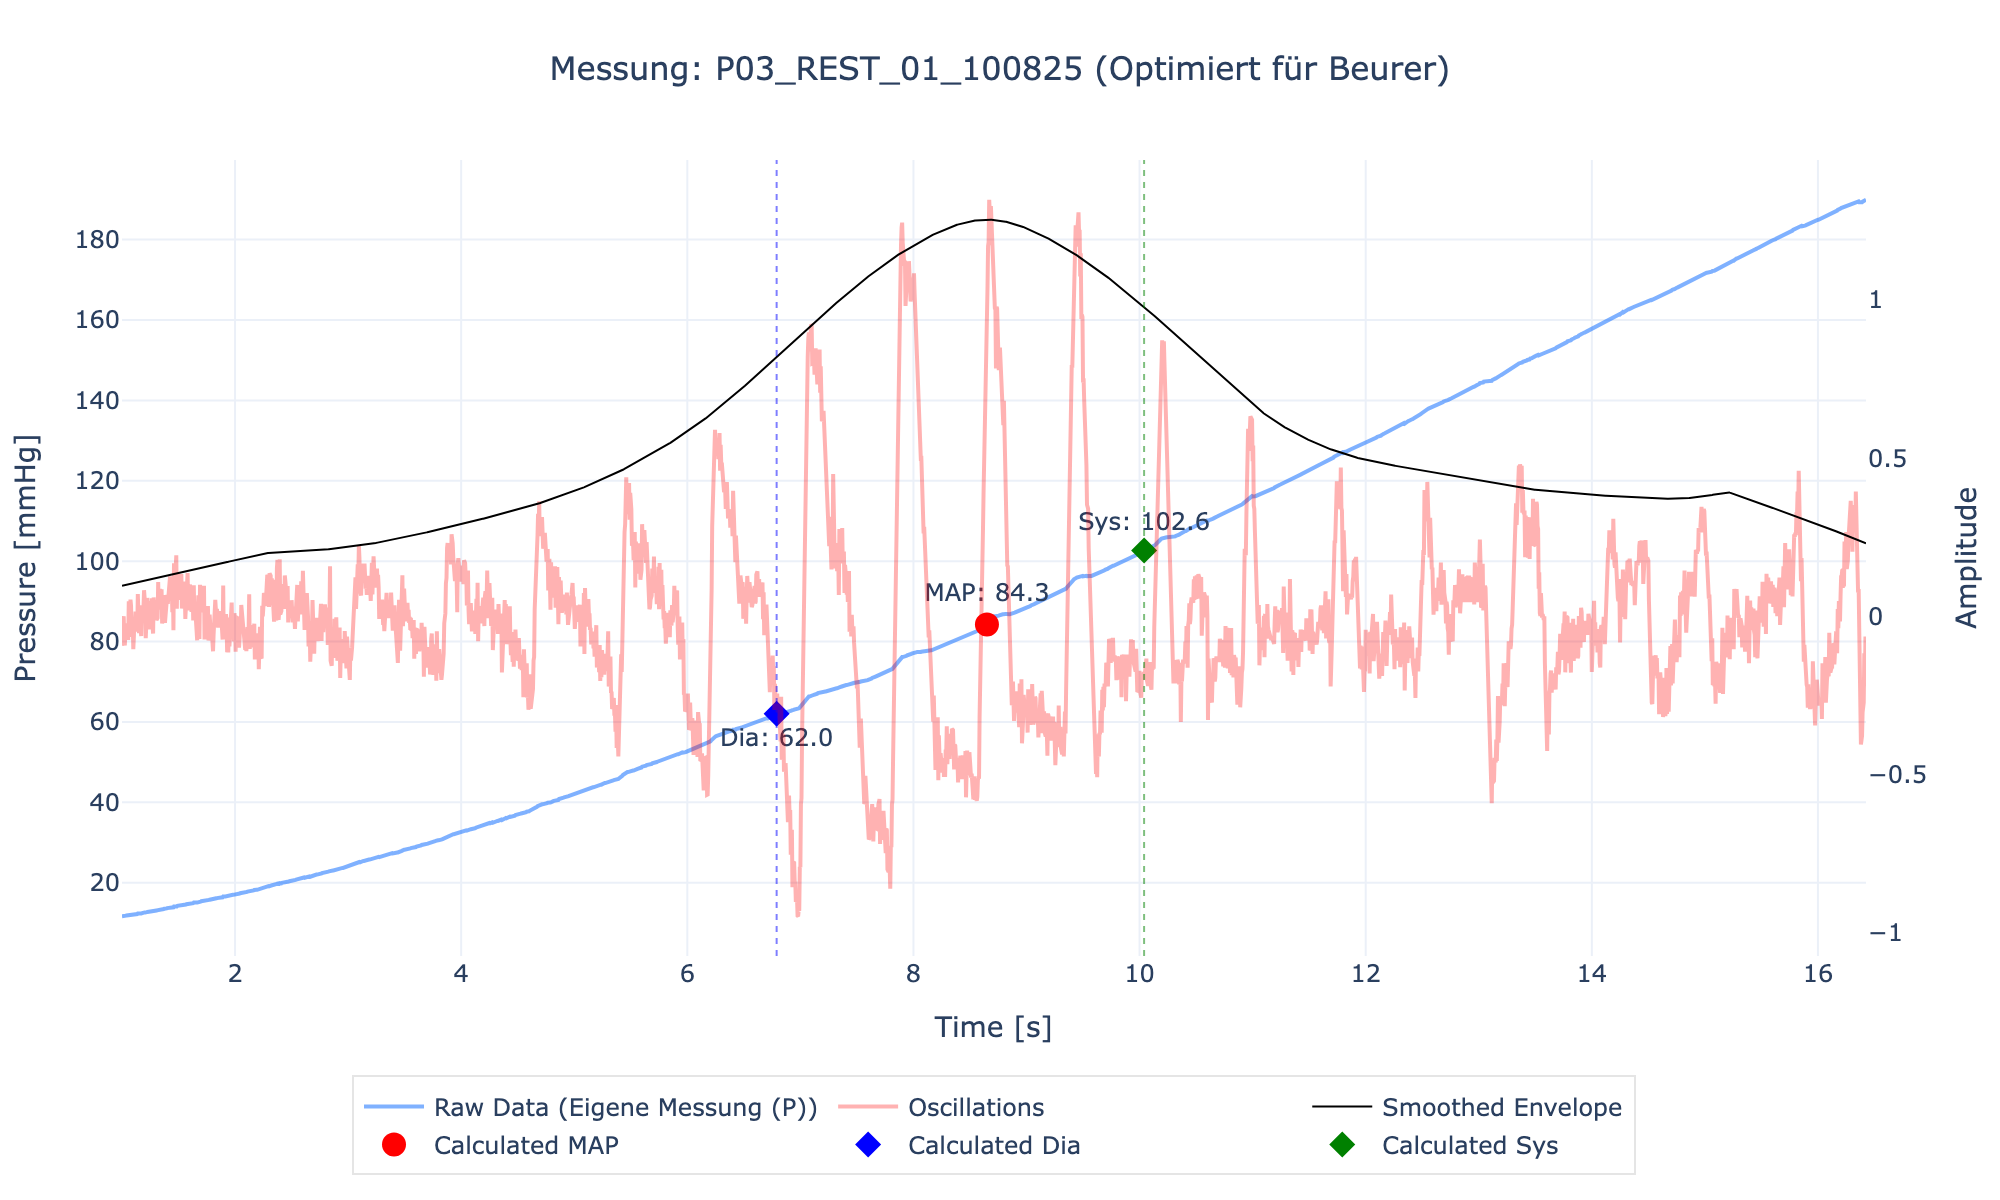
\includegraphics[width=\textwidth]{images/P03_REST_01_100825_beurer.png}
        \caption{Optimiert für Beurer}
    \end{subfigure}
    \hfill
    \begin{subfigure}[b]{0.48\textwidth}
        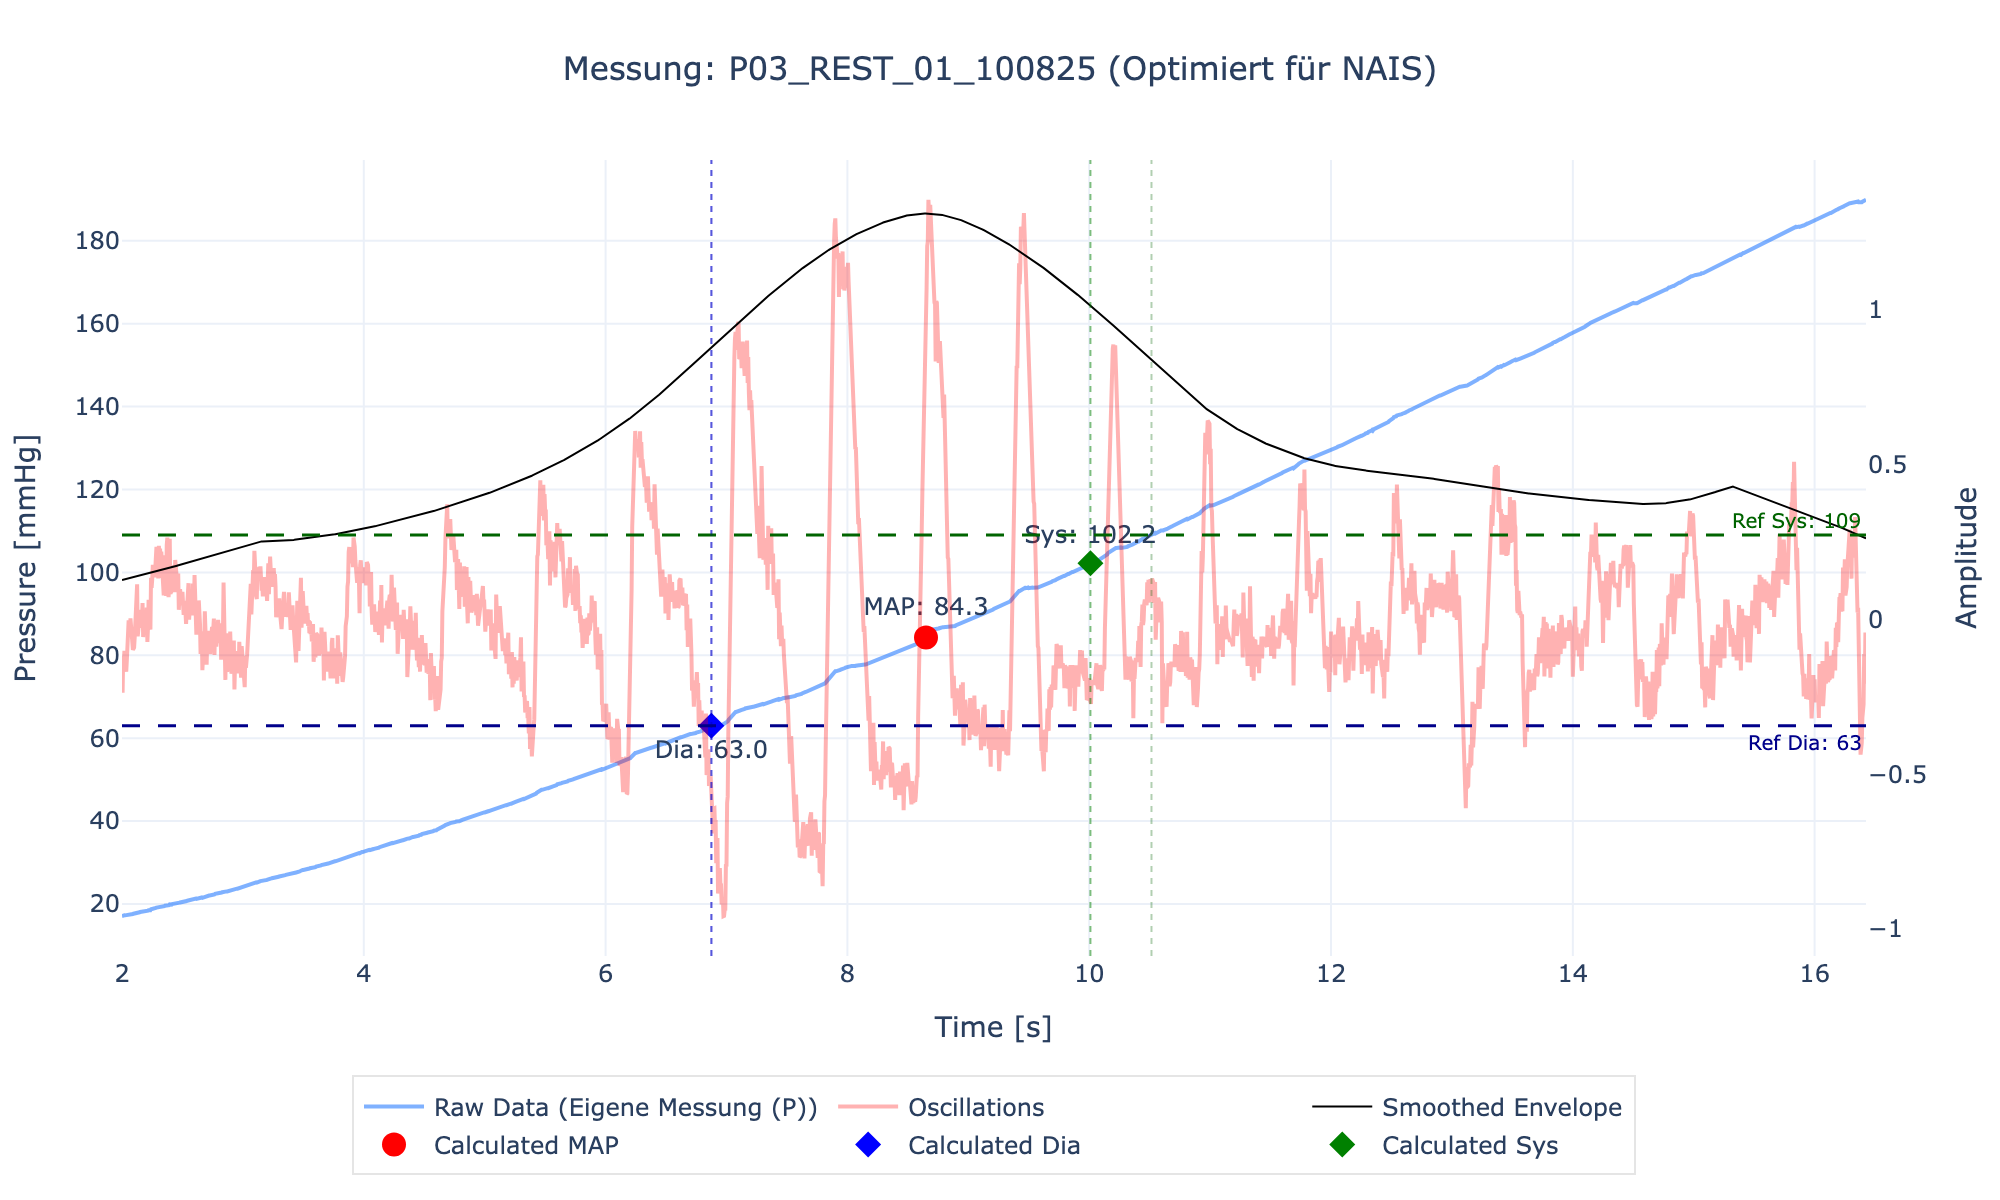
\includegraphics[width=\textwidth]{images/P03_REST_01_100825_nais.png}
        \caption{Optimiert für NAIS}
    \end{subfigure}
    \caption{Einzelauswertung der Messung P03\_REST\_01\_100825 mit verschiedenen Parametersätzen.}
\end{figure}
\newpage

\subsection*{Messung: P03\_REST\_02\_160925}
\begin{figure}[H]
    \centering
    \begin{subfigure}[b]{0.8\textwidth}
        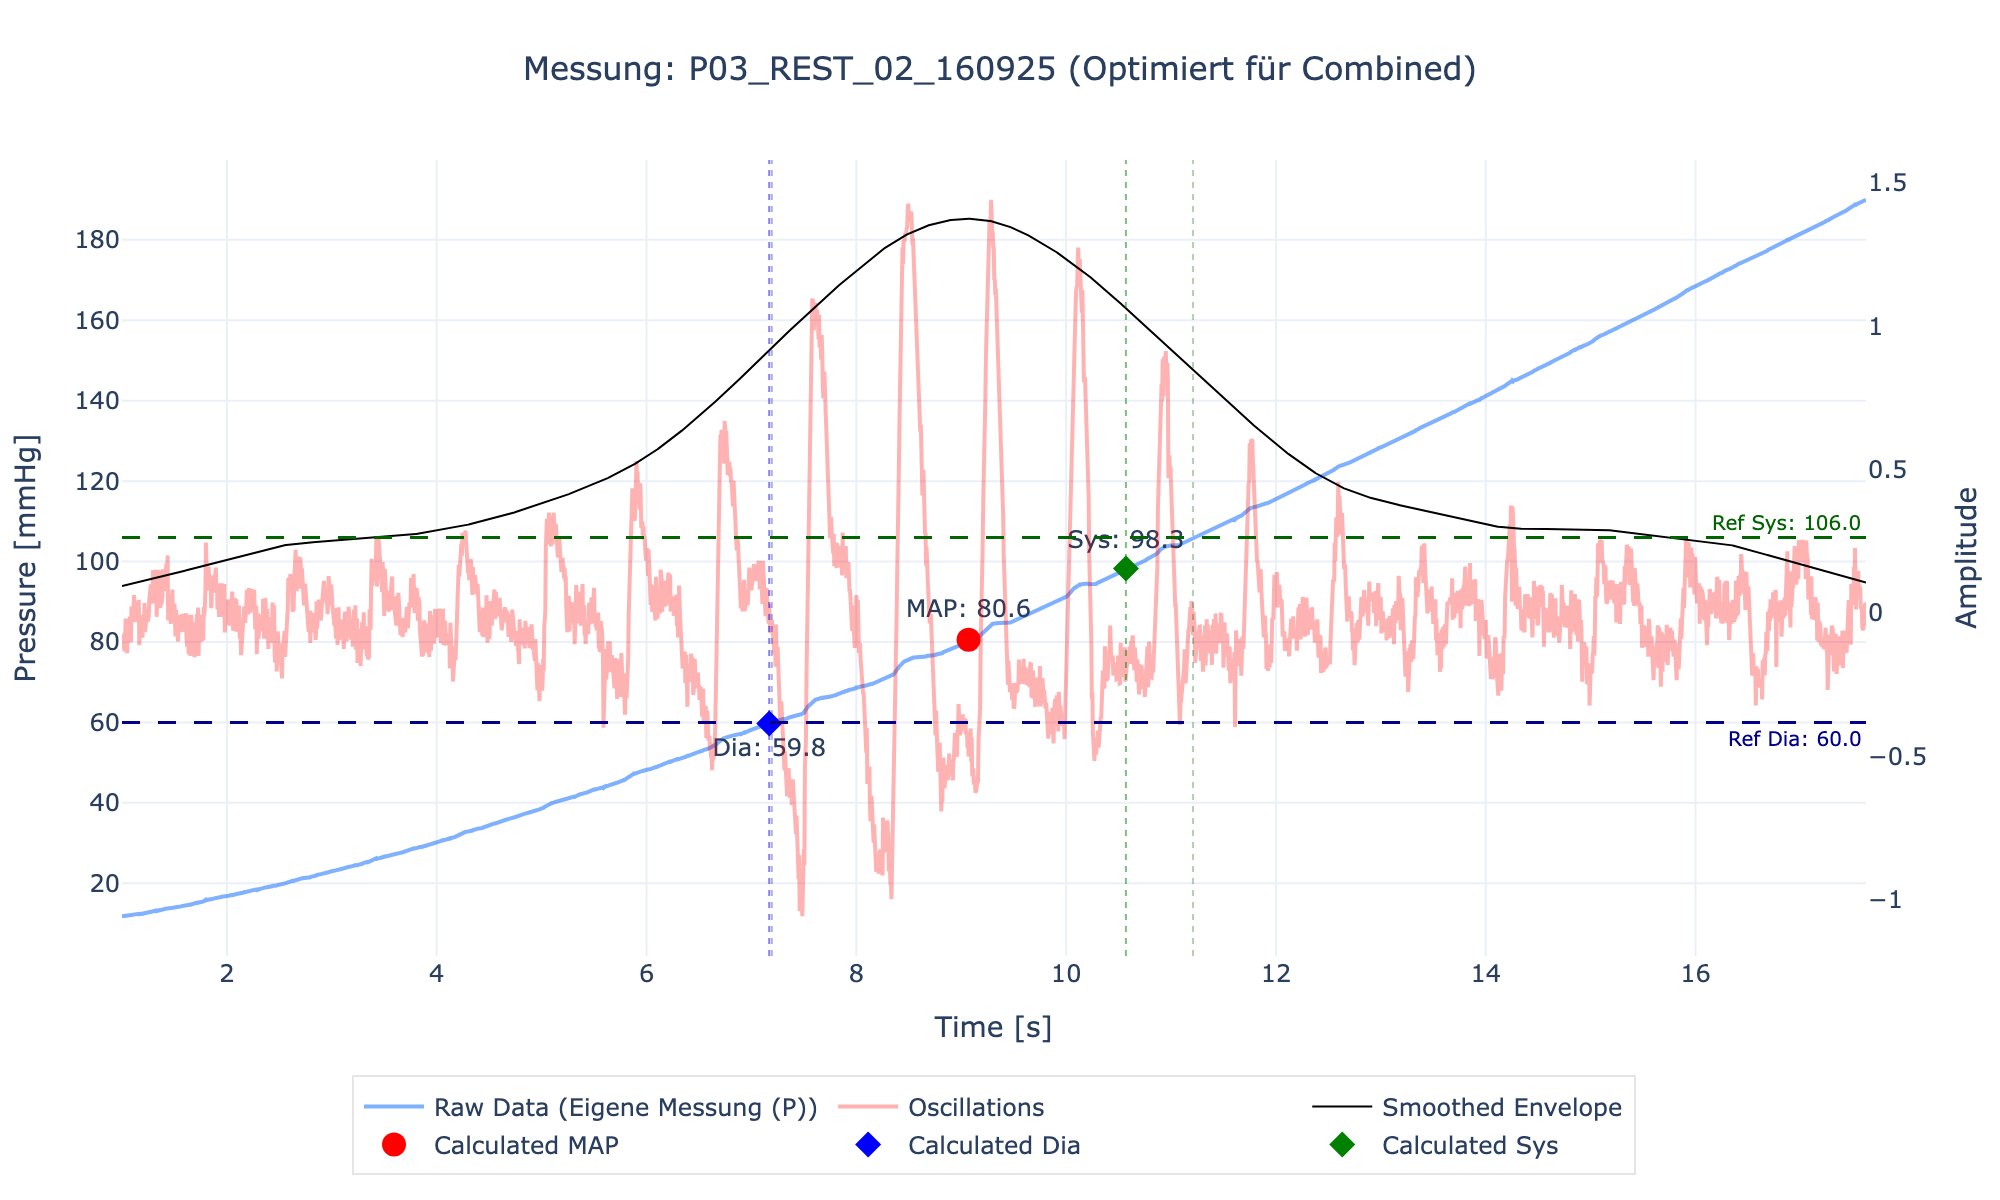
\includegraphics[width=\textwidth]{images/P03_REST_02_160925_combined.png}
        \caption{Optimiert für Beurer und NAIS (Kombiniert)}
    \end{subfigure} \\
    \begin{subfigure}[b]{0.48\textwidth}
        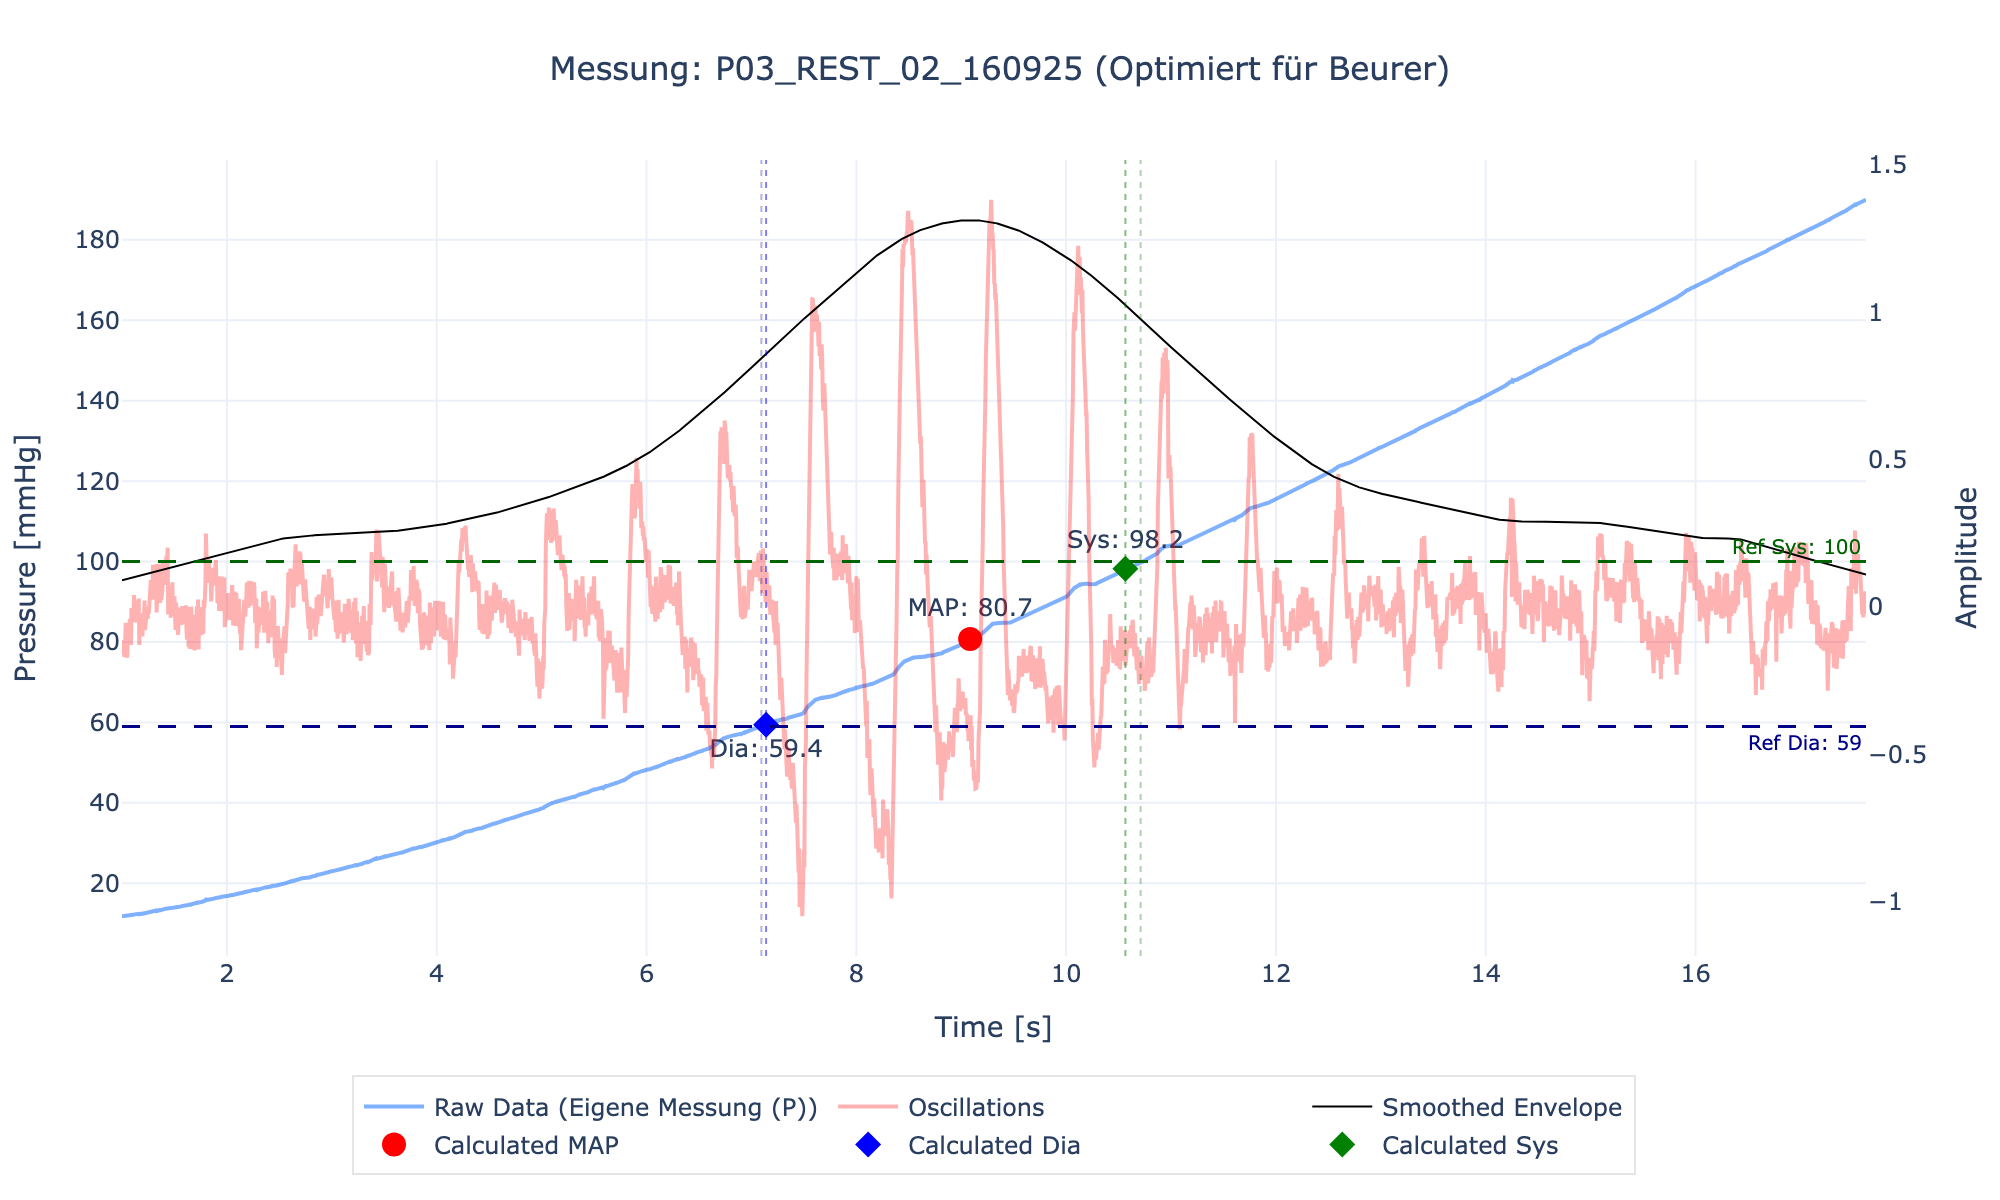
\includegraphics[width=\textwidth]{images/P03_REST_02_160925_beurer.png}
        \caption{Optimiert für Beurer}
    \end{subfigure}
    \hfill
    \begin{subfigure}[b]{0.48\textwidth}
        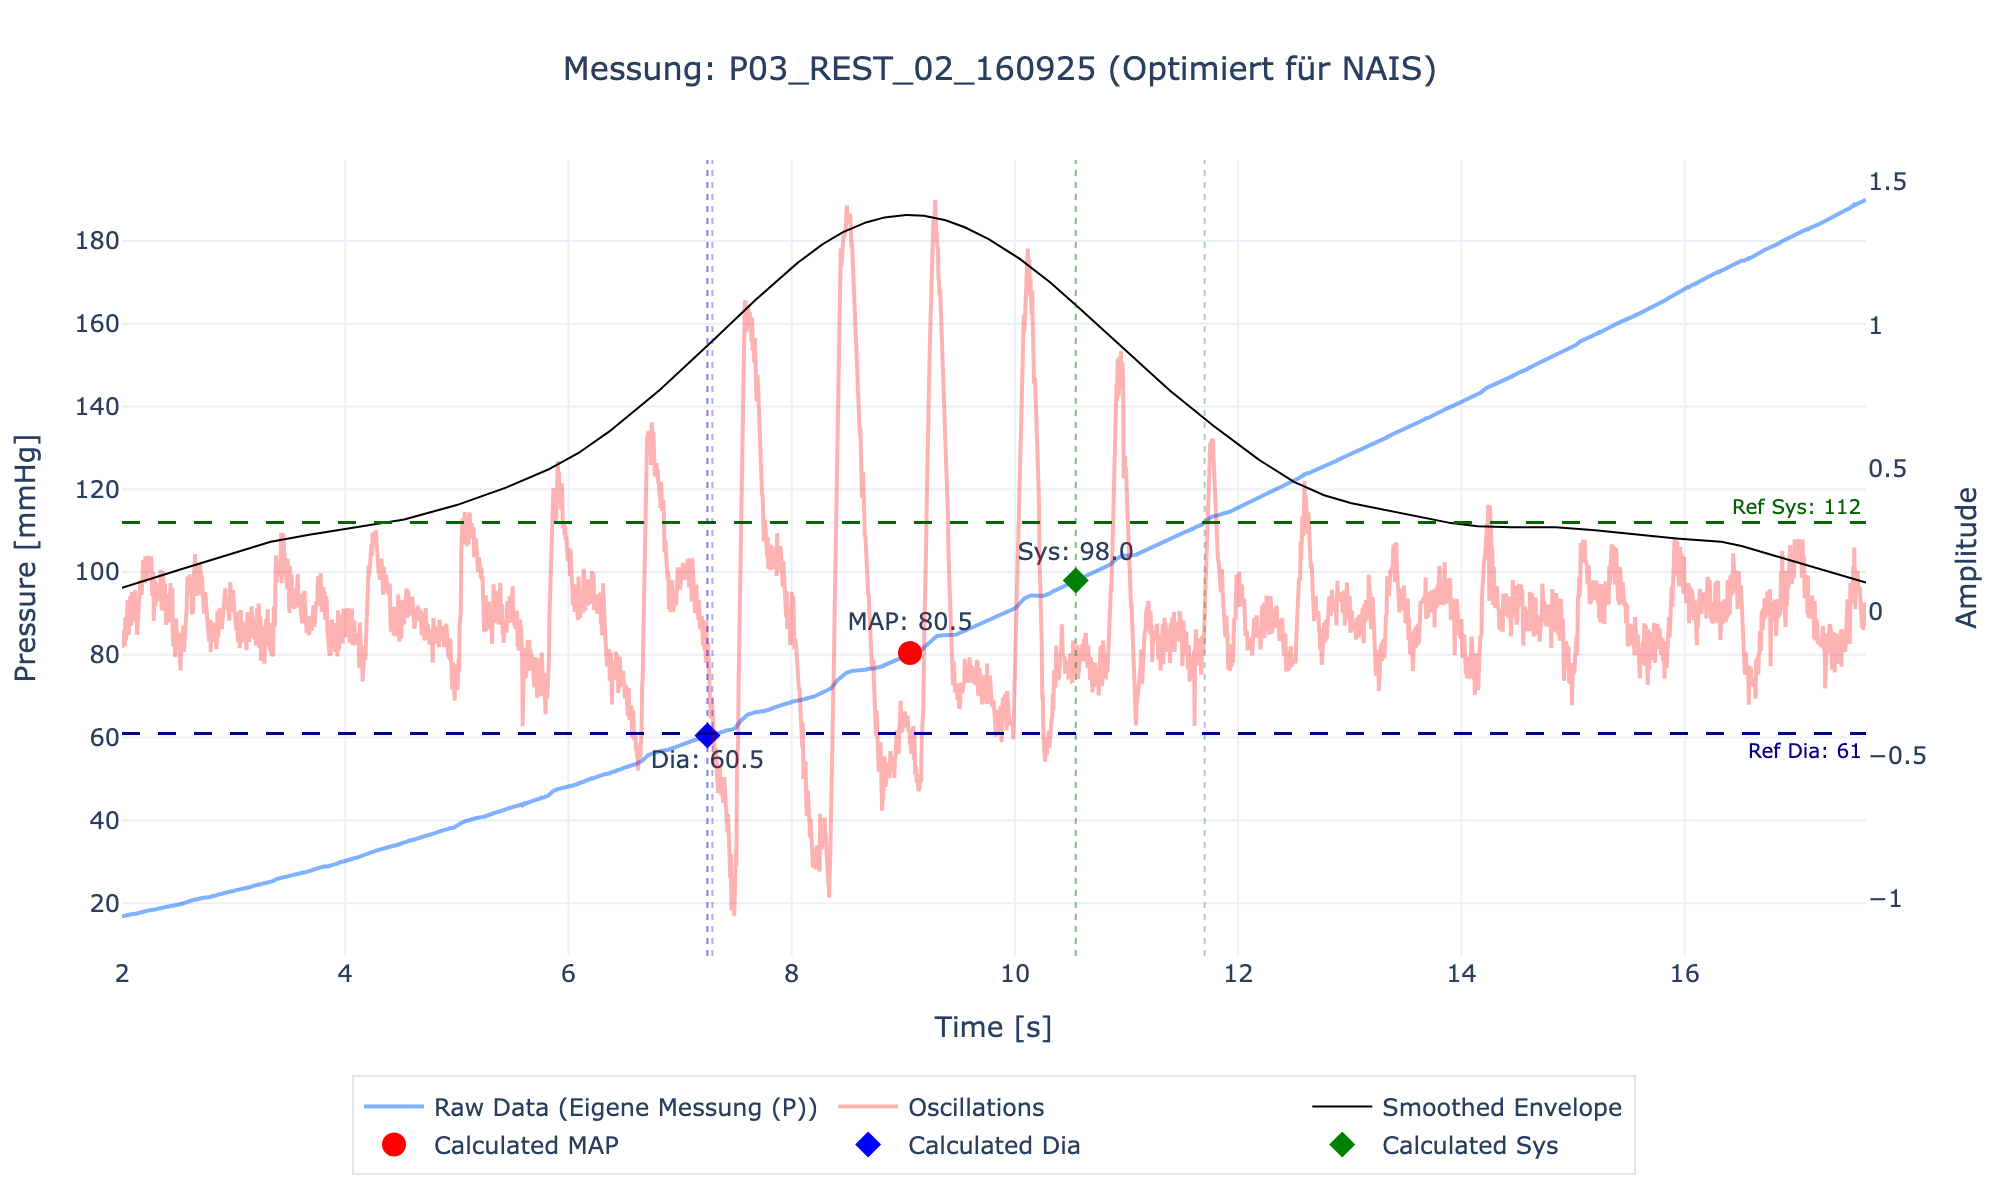
\includegraphics[width=\textwidth]{images/P03_REST_02_160925_nais.png}
        \caption{Optimiert für NAIS}
    \end{subfigure}
    \caption{Einzelauswertung der Messung P03\_REST\_02\_160925 mit verschiedenen Parametersätzen.}
\end{figure}
\newpage

\subsection*{Messung: P04\_ACTIV\_01\_160925}
\begin{figure}[H]
    \centering
    \begin{subfigure}[b]{0.8\textwidth}
        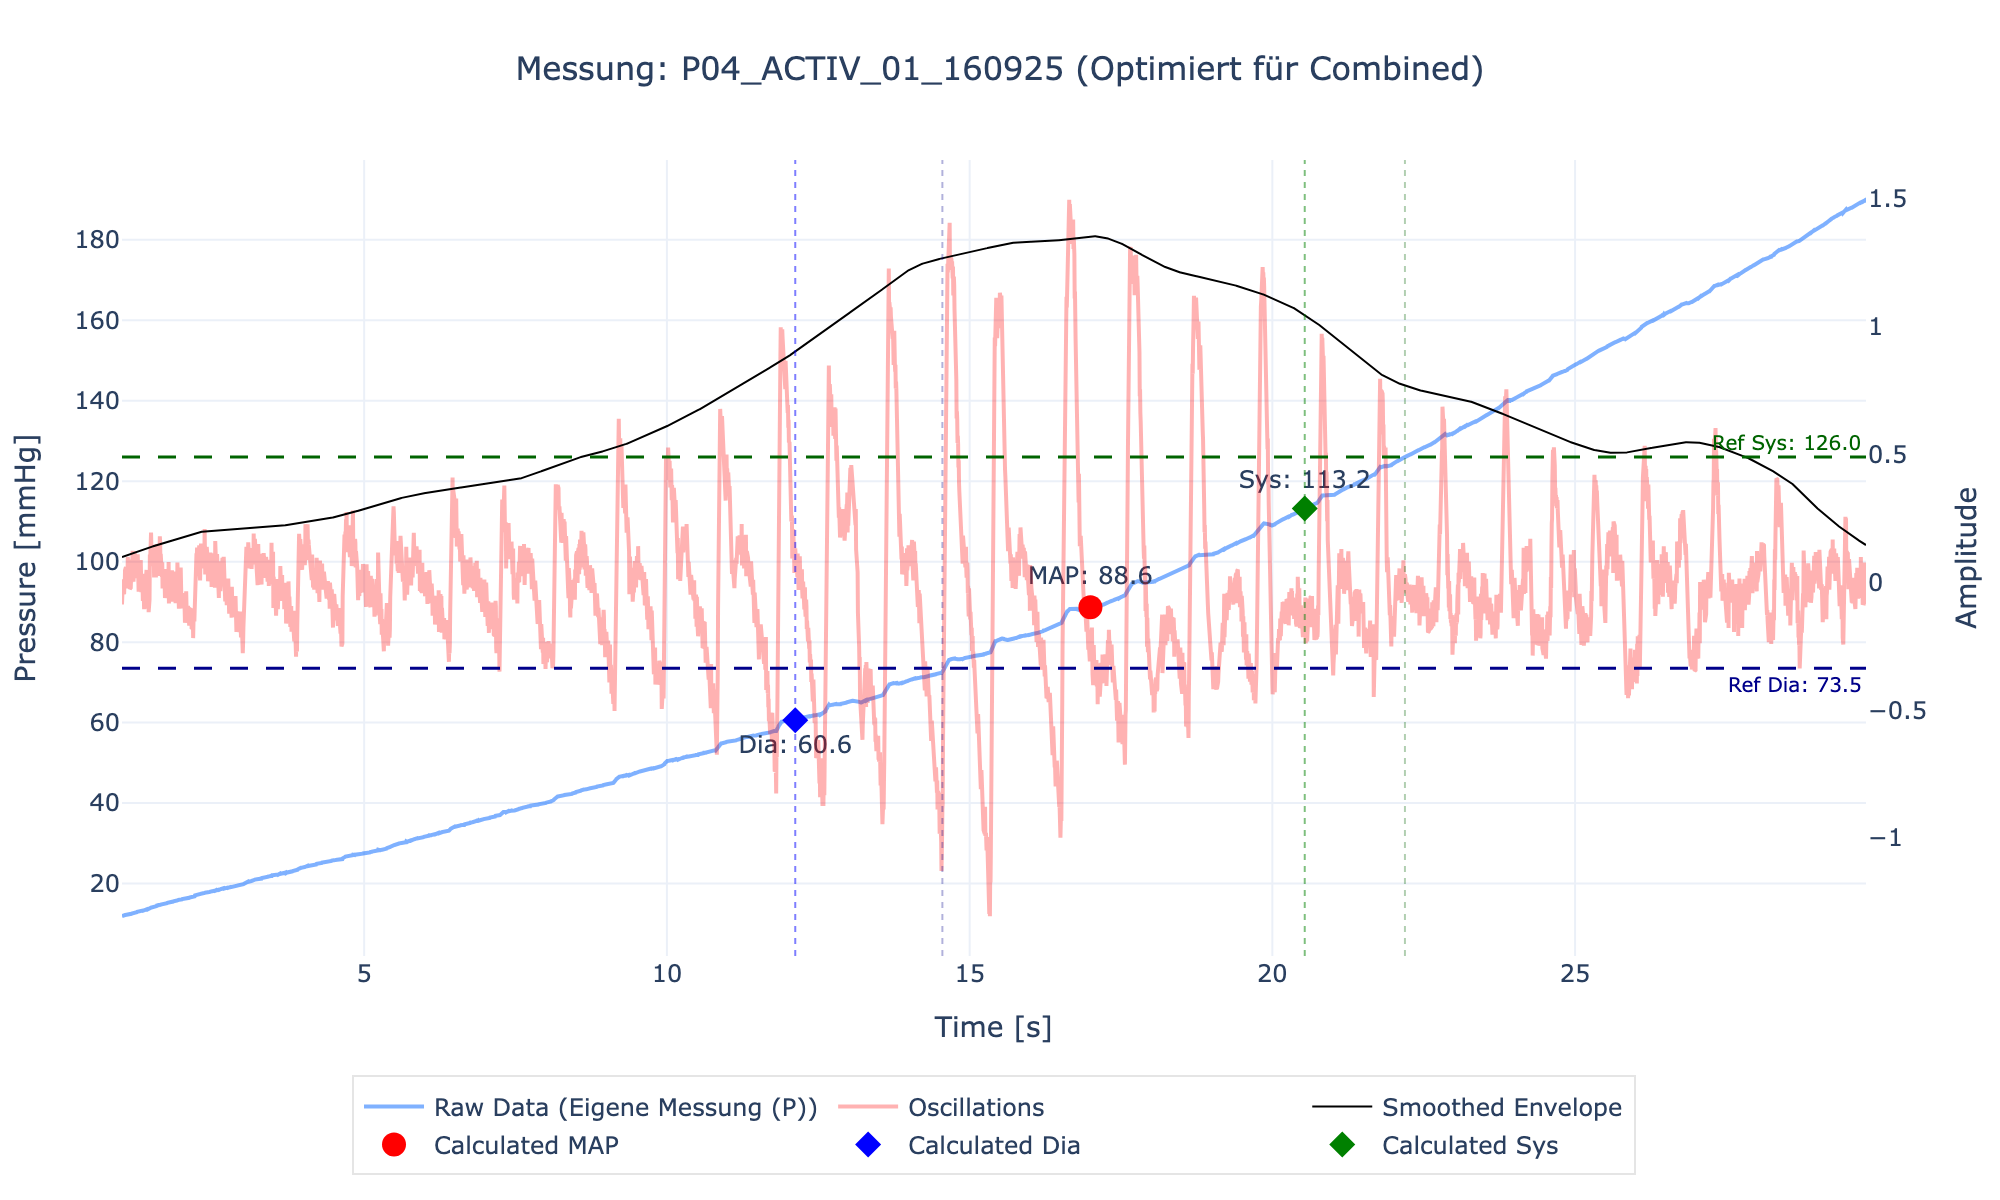
\includegraphics[width=\textwidth]{images/P04_ACTIV_01_160925_combined.png}
        \caption{Optimiert für Beurer und NAIS (Kombiniert)}
    \end{subfigure} \\
    \begin{subfigure}[b]{0.48\textwidth}
        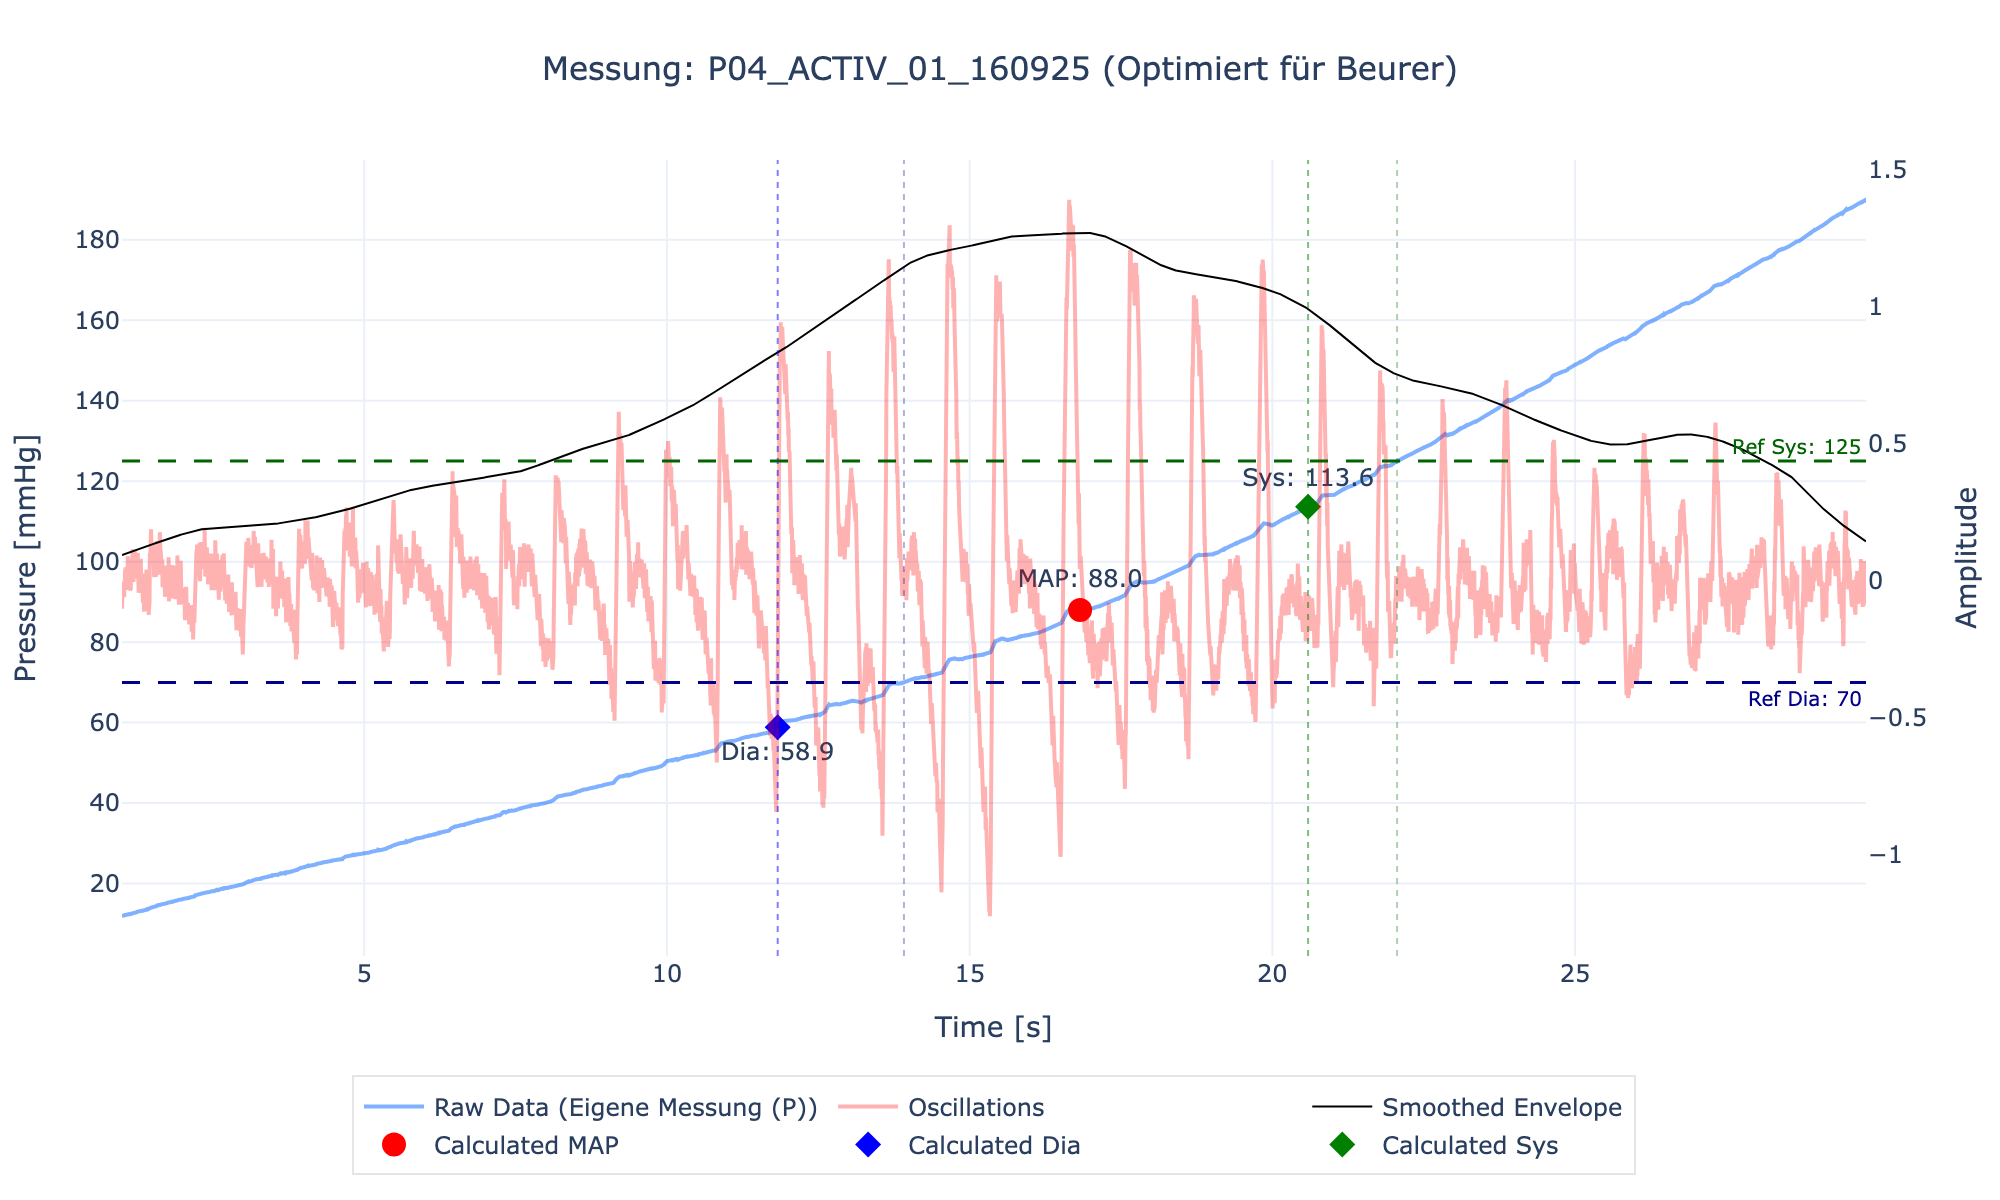
\includegraphics[width=\textwidth]{images/P04_ACTIV_01_160925_beurer.png}
        \caption{Optimiert für Beurer}
    \end{subfigure}
    \hfill
    \begin{subfigure}[b]{0.48\textwidth}
        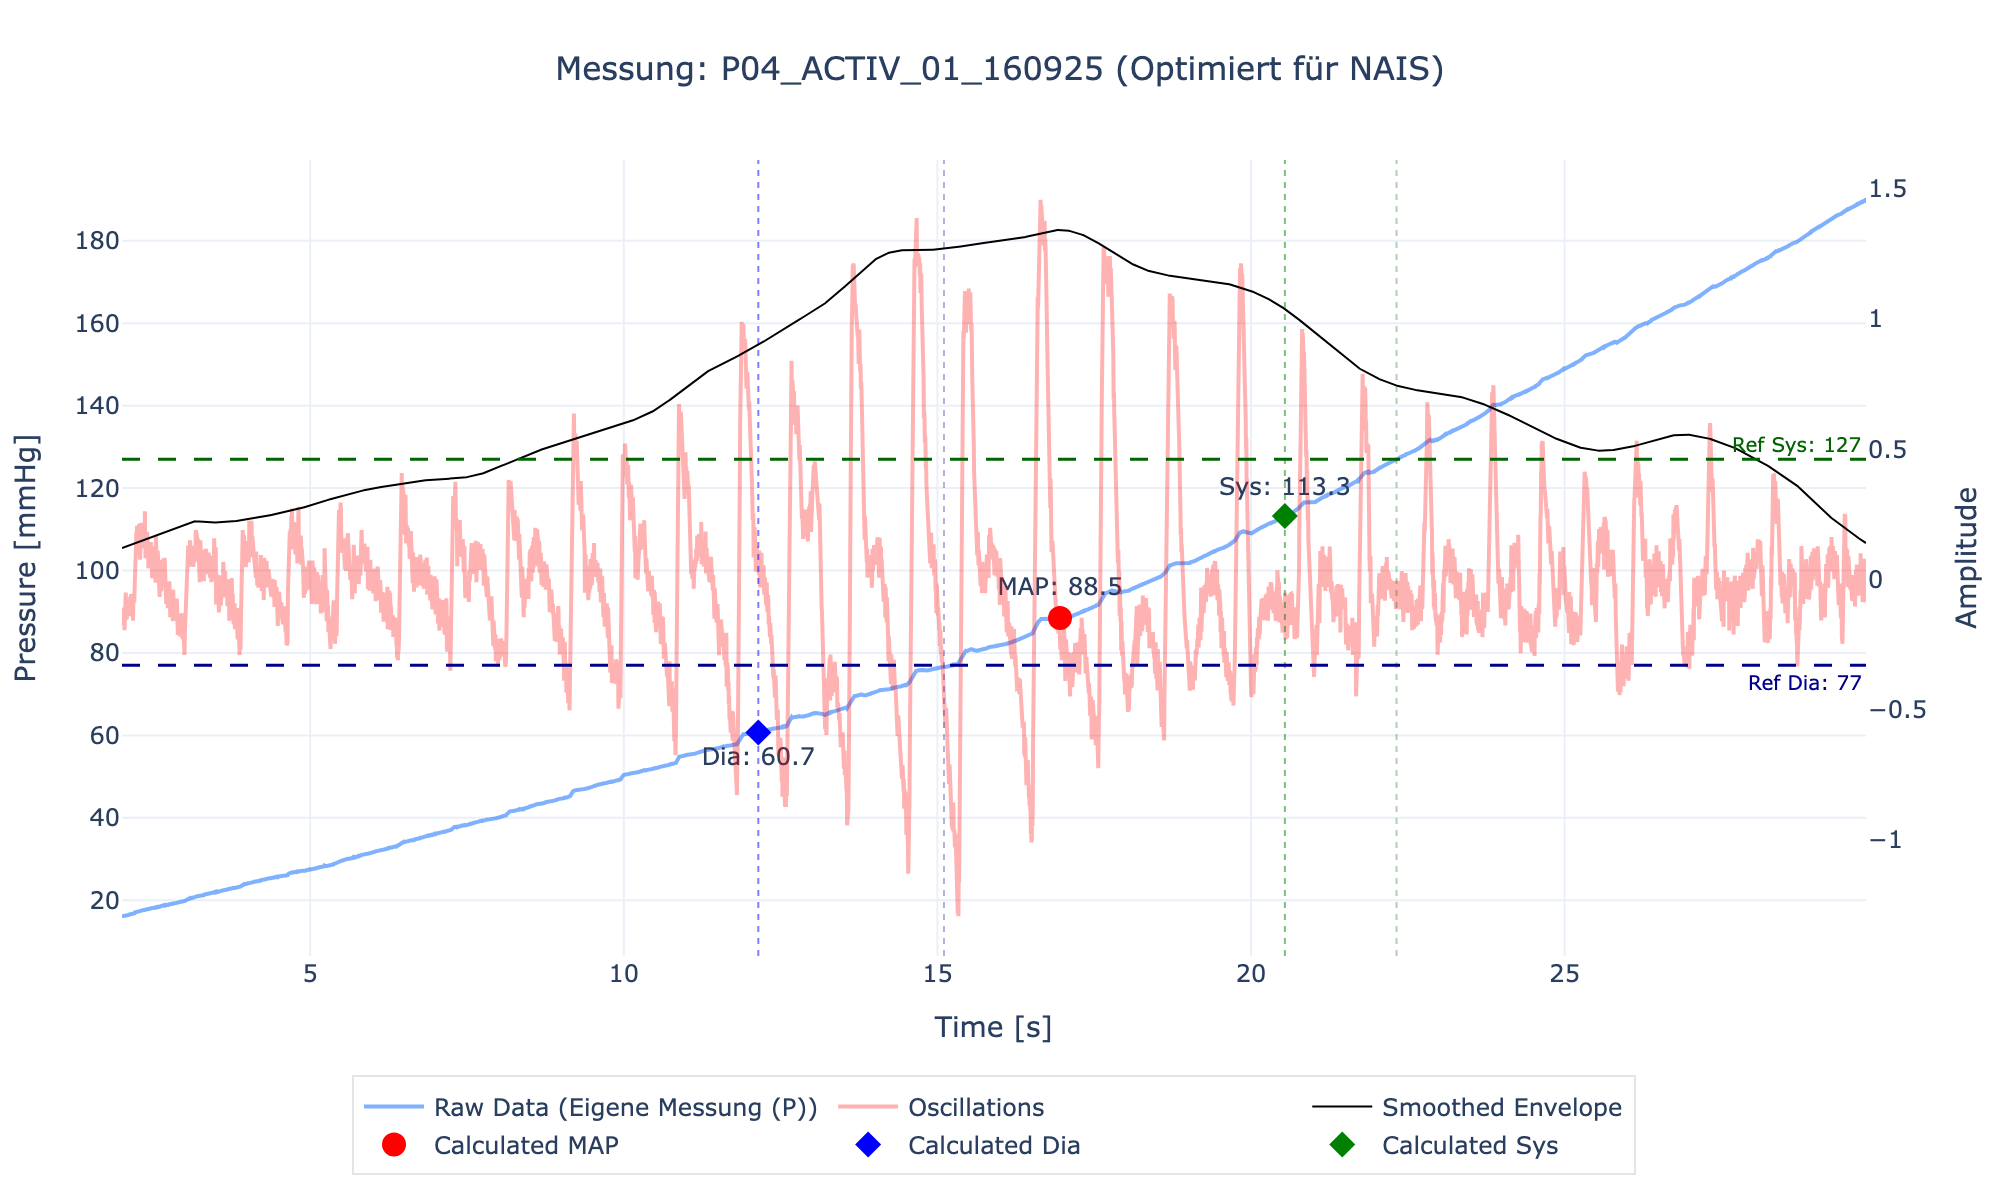
\includegraphics[width=\textwidth]{images/P04_ACTIV_01_160925_nais.png}
        \caption{Optimiert für NAIS}
    \end{subfigure}
    \caption{Einzelauswertung der Messung P04\_ACTIV\_01\_160925 mit verschiedenen Parametersätzen.}
\end{figure}
\newpage

\subsection*{Messung: P04\_REST\_01\_160925}
\begin{figure}[H]
    \centering
    \begin{subfigure}[b]{0.8\textwidth}
        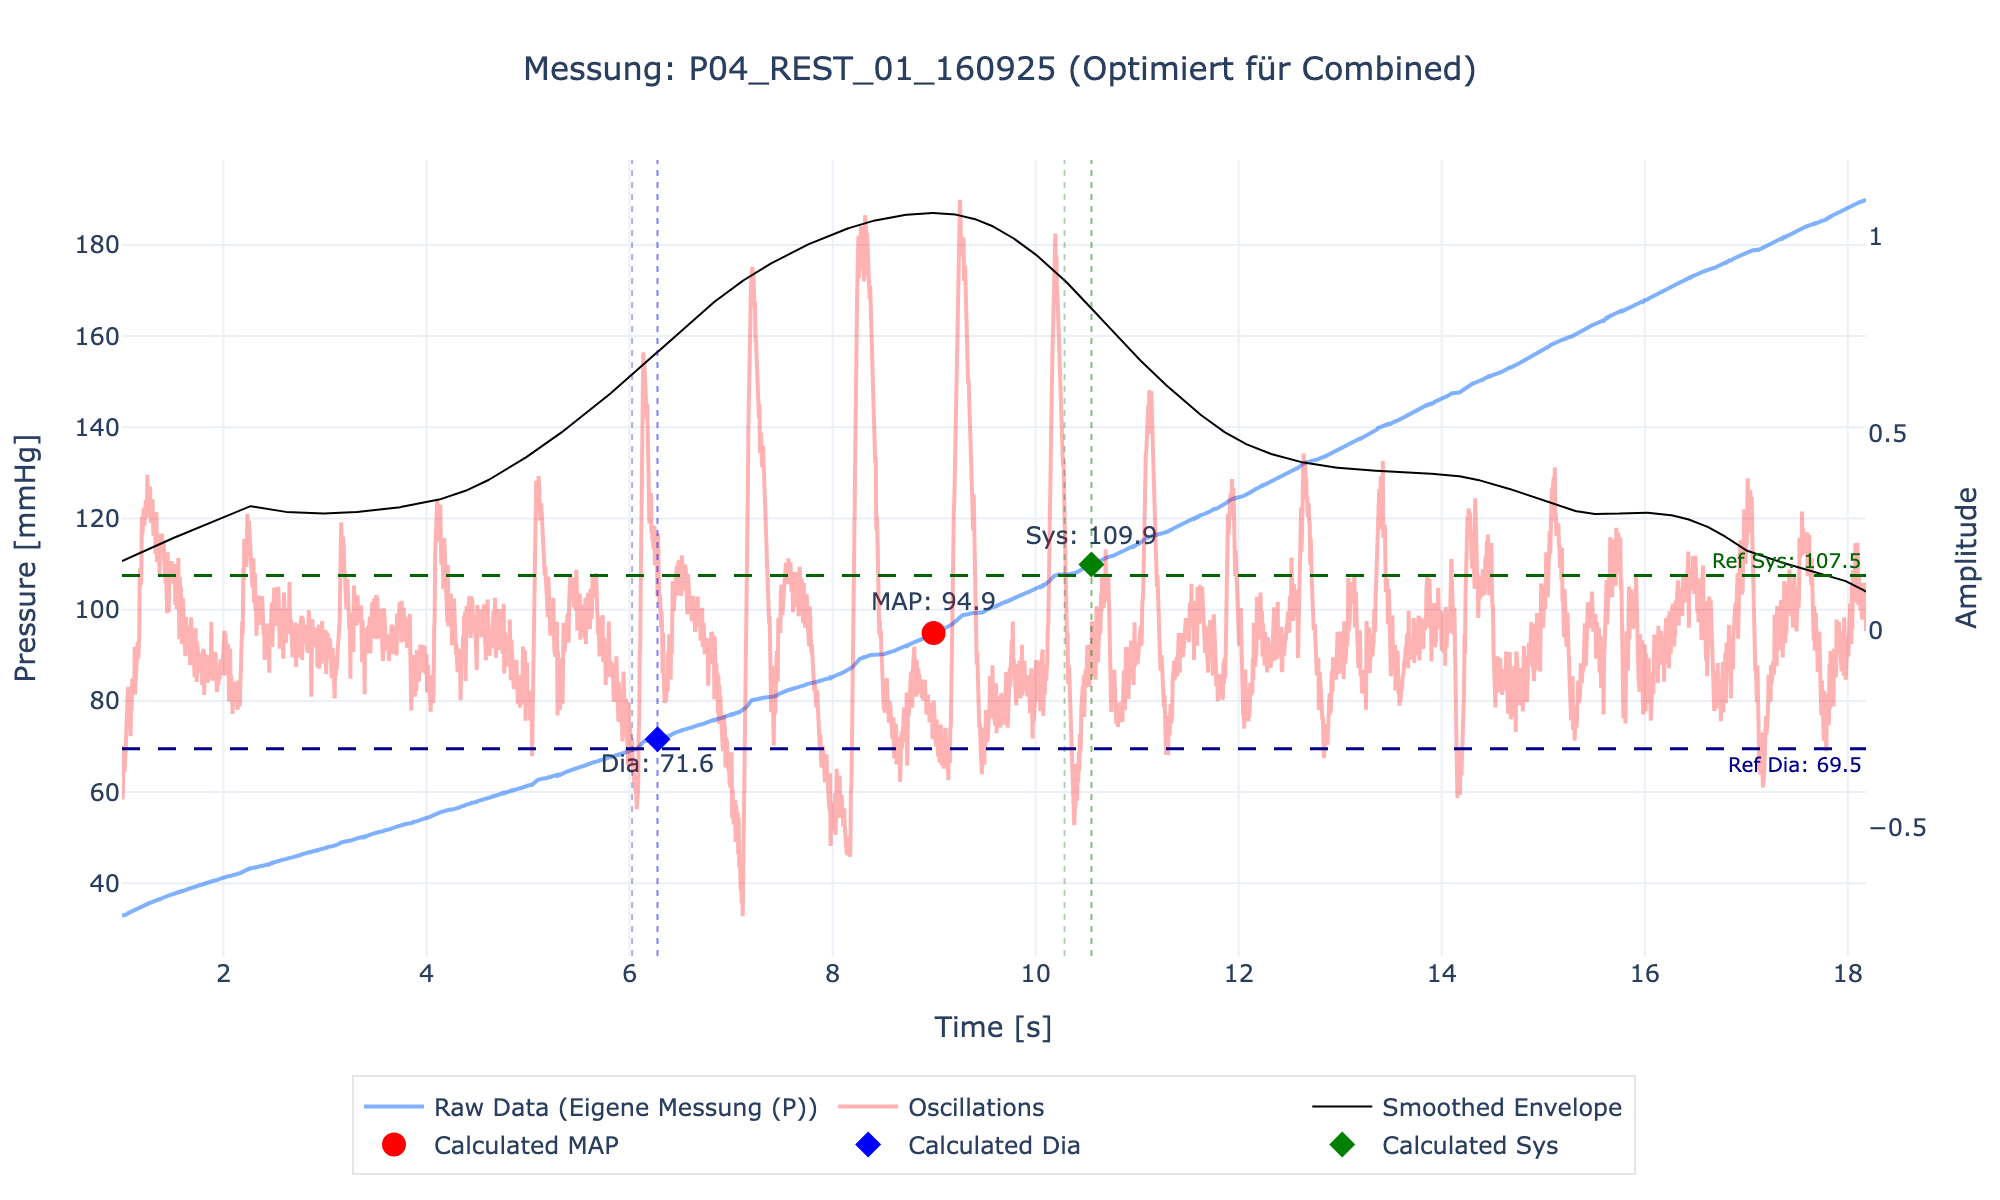
\includegraphics[width=\textwidth]{images/P04_REST_01_160925_combined.png}
        \caption{Optimiert für Beurer und NAIS (Kombiniert)}
    \end{subfigure} \\
    \begin{subfigure}[b]{0.48\textwidth}
        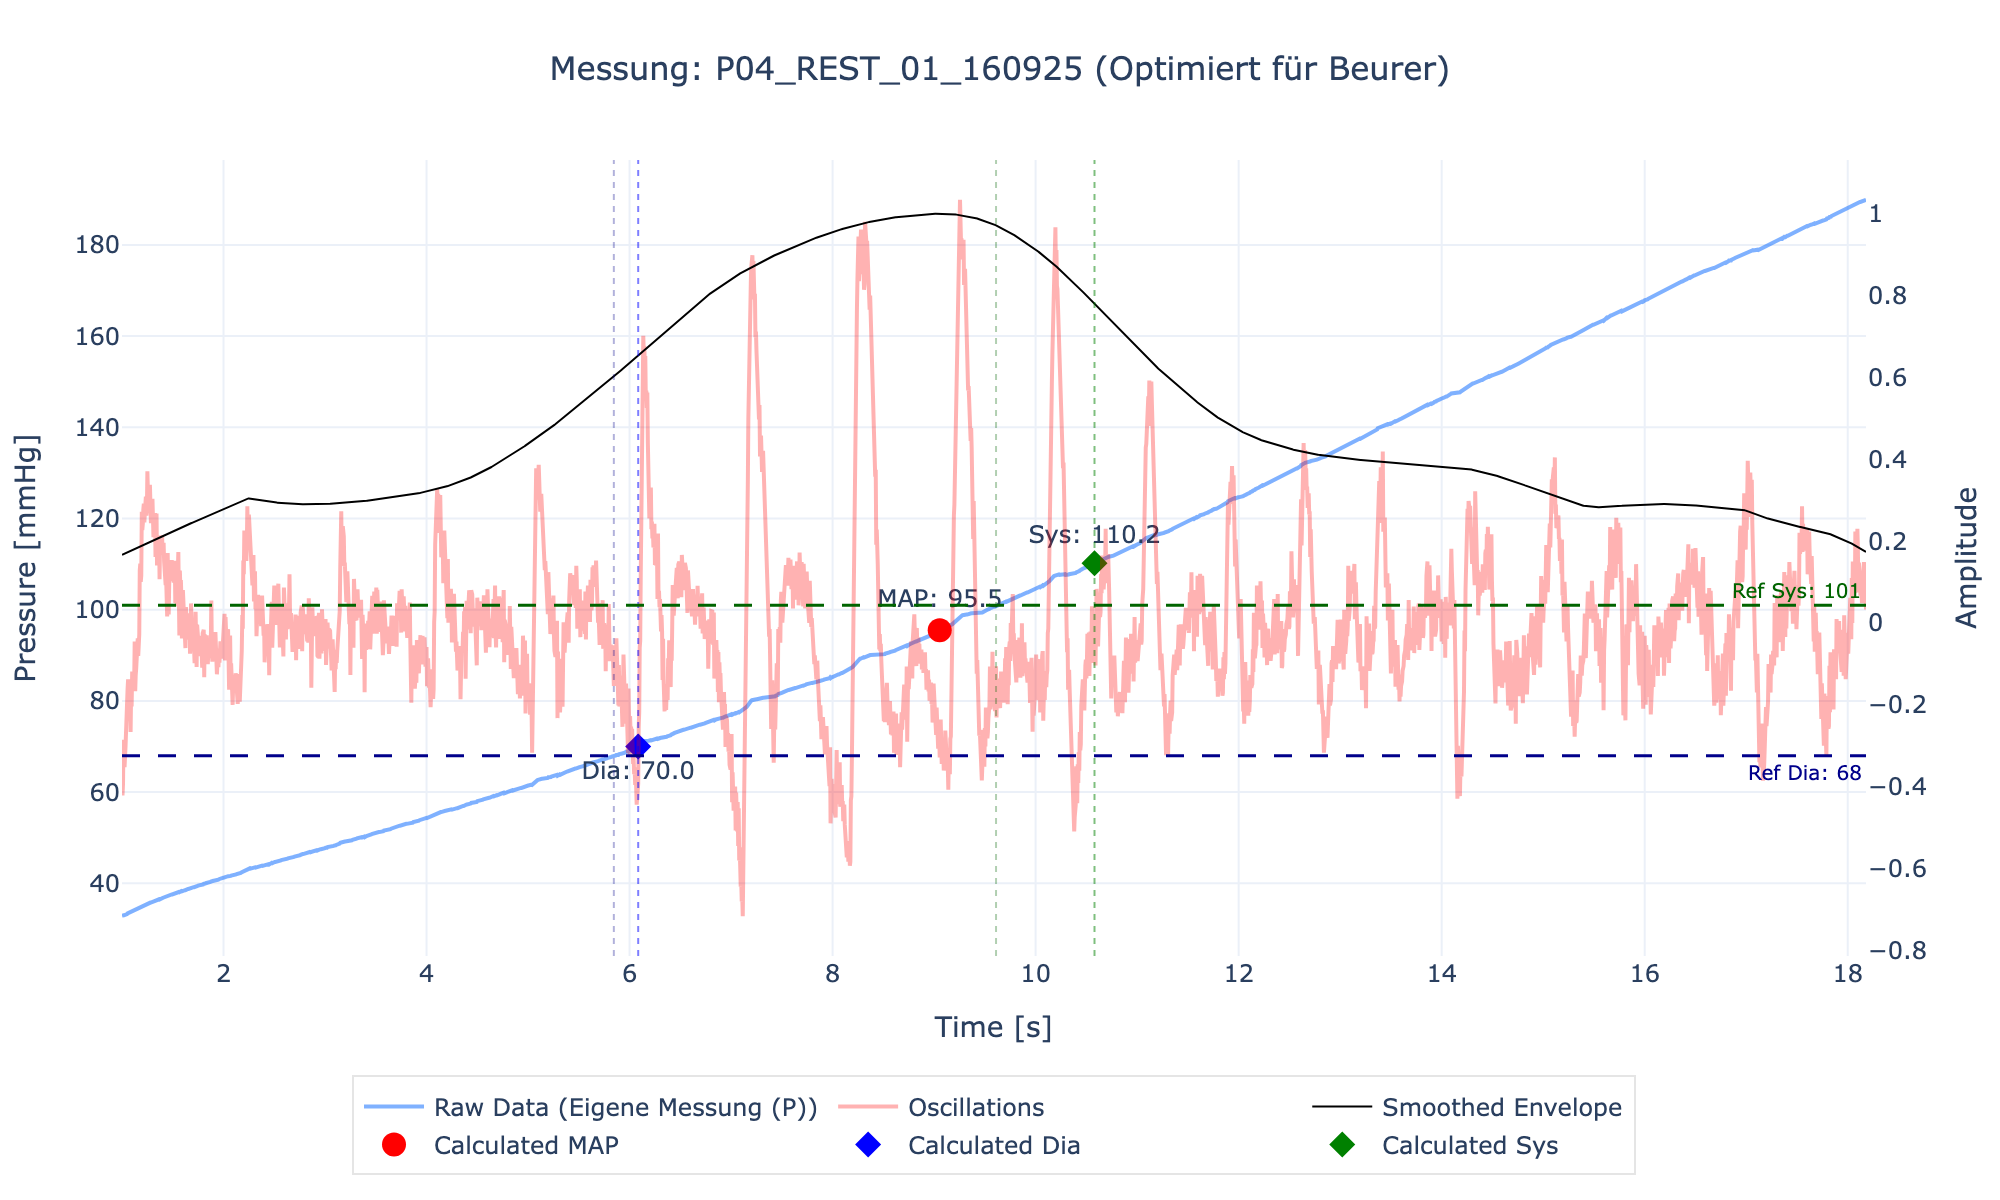
\includegraphics[width=\textwidth]{images/P04_REST_01_160925_beurer.png}
        \caption{Optimiert für Beurer}
    \end{subfigure}
    \hfill
    \begin{subfigure}[b]{0.48\textwidth}
        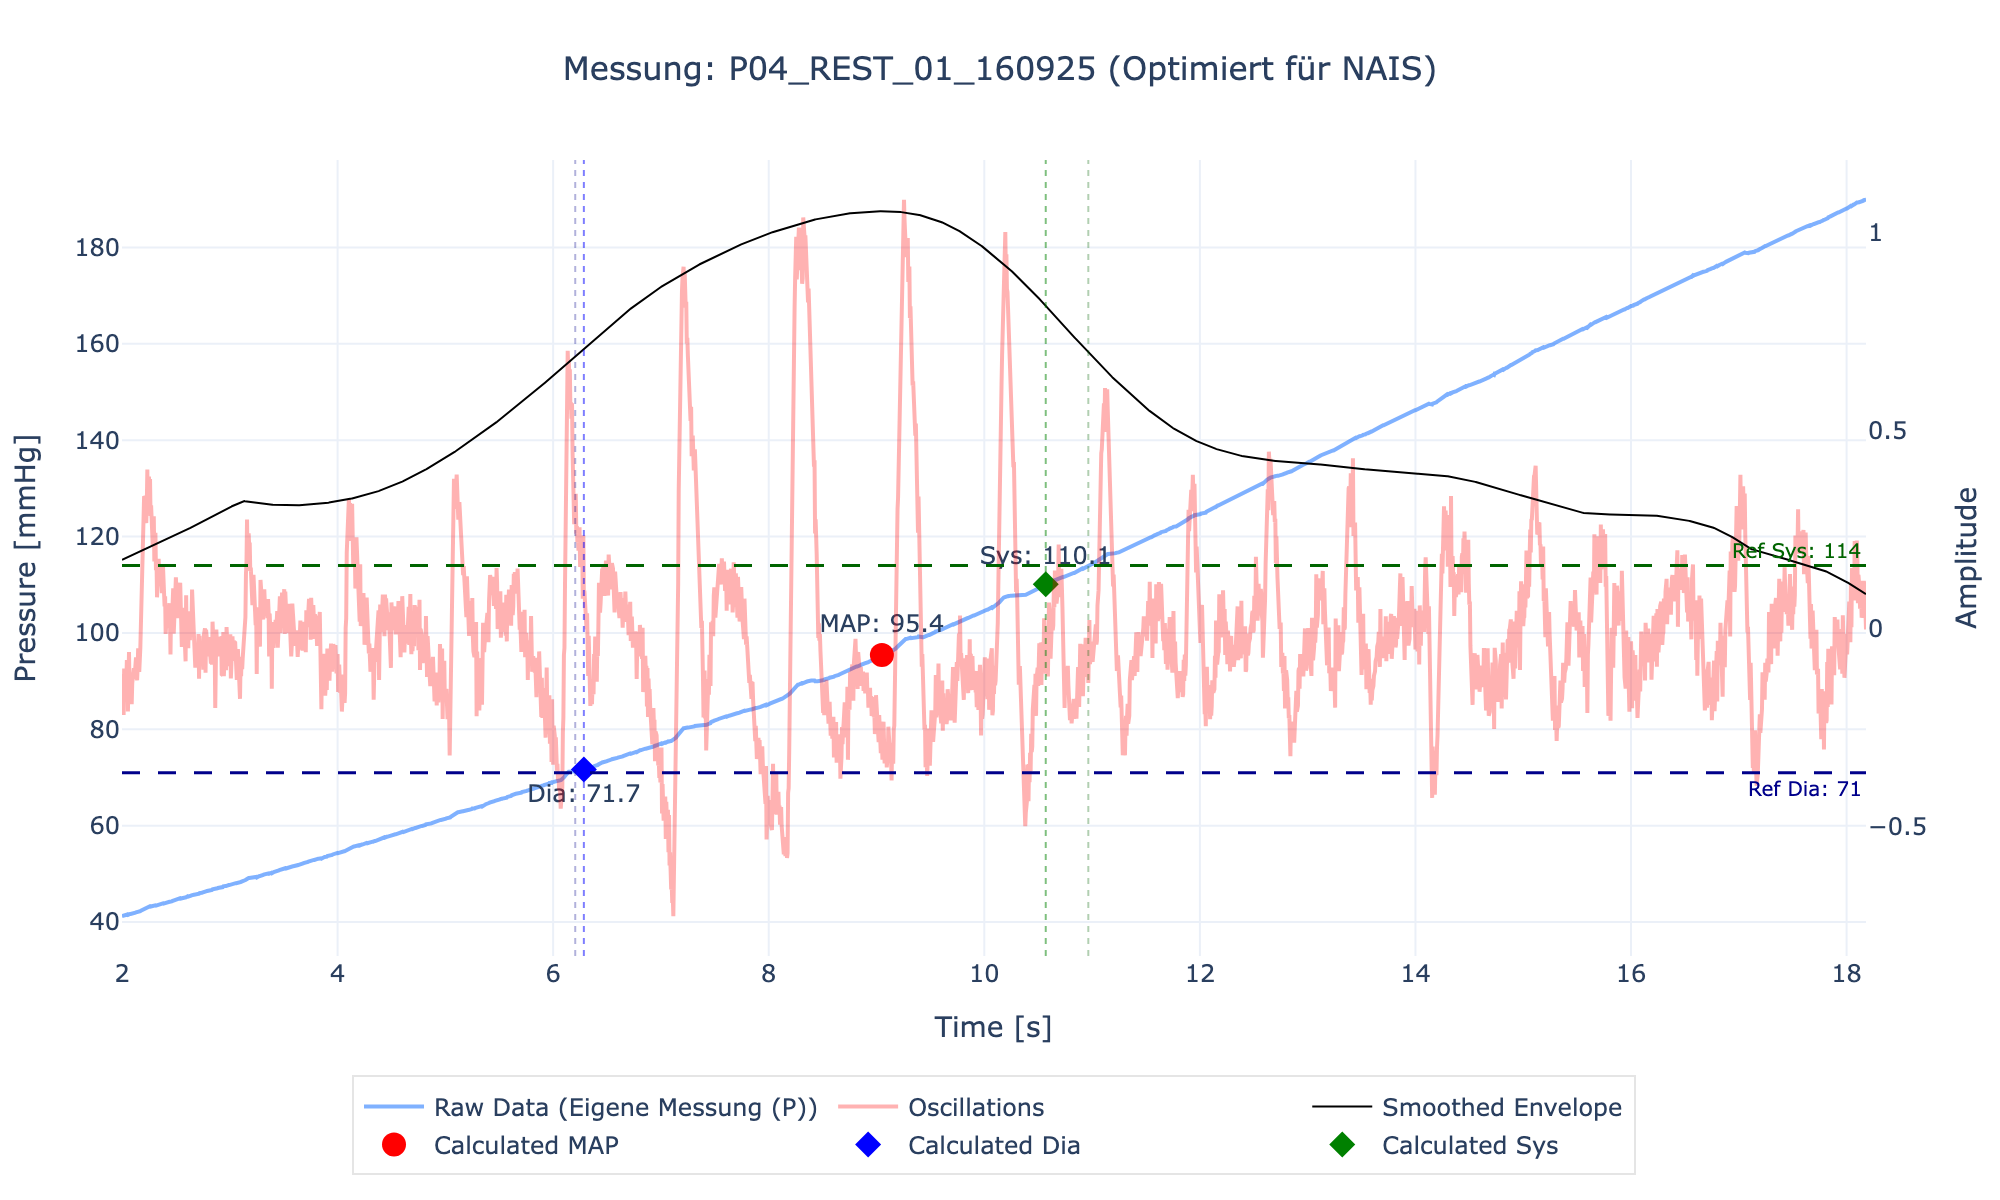
\includegraphics[width=\textwidth]{images/P04_REST_01_160925_nais.png}
        \caption{Optimiert für NAIS}
    \end{subfigure}
    \caption{Einzelauswertung der Messung P04\_REST\_01\_160925 mit verschiedenen Parametersätzen.}
\end{figure}
\newpage

\subsection*{Messung: P05\_ACTIV\_01\_210925}
\begin{figure}[H]
    \centering
    \begin{subfigure}[b]{0.8\textwidth}
        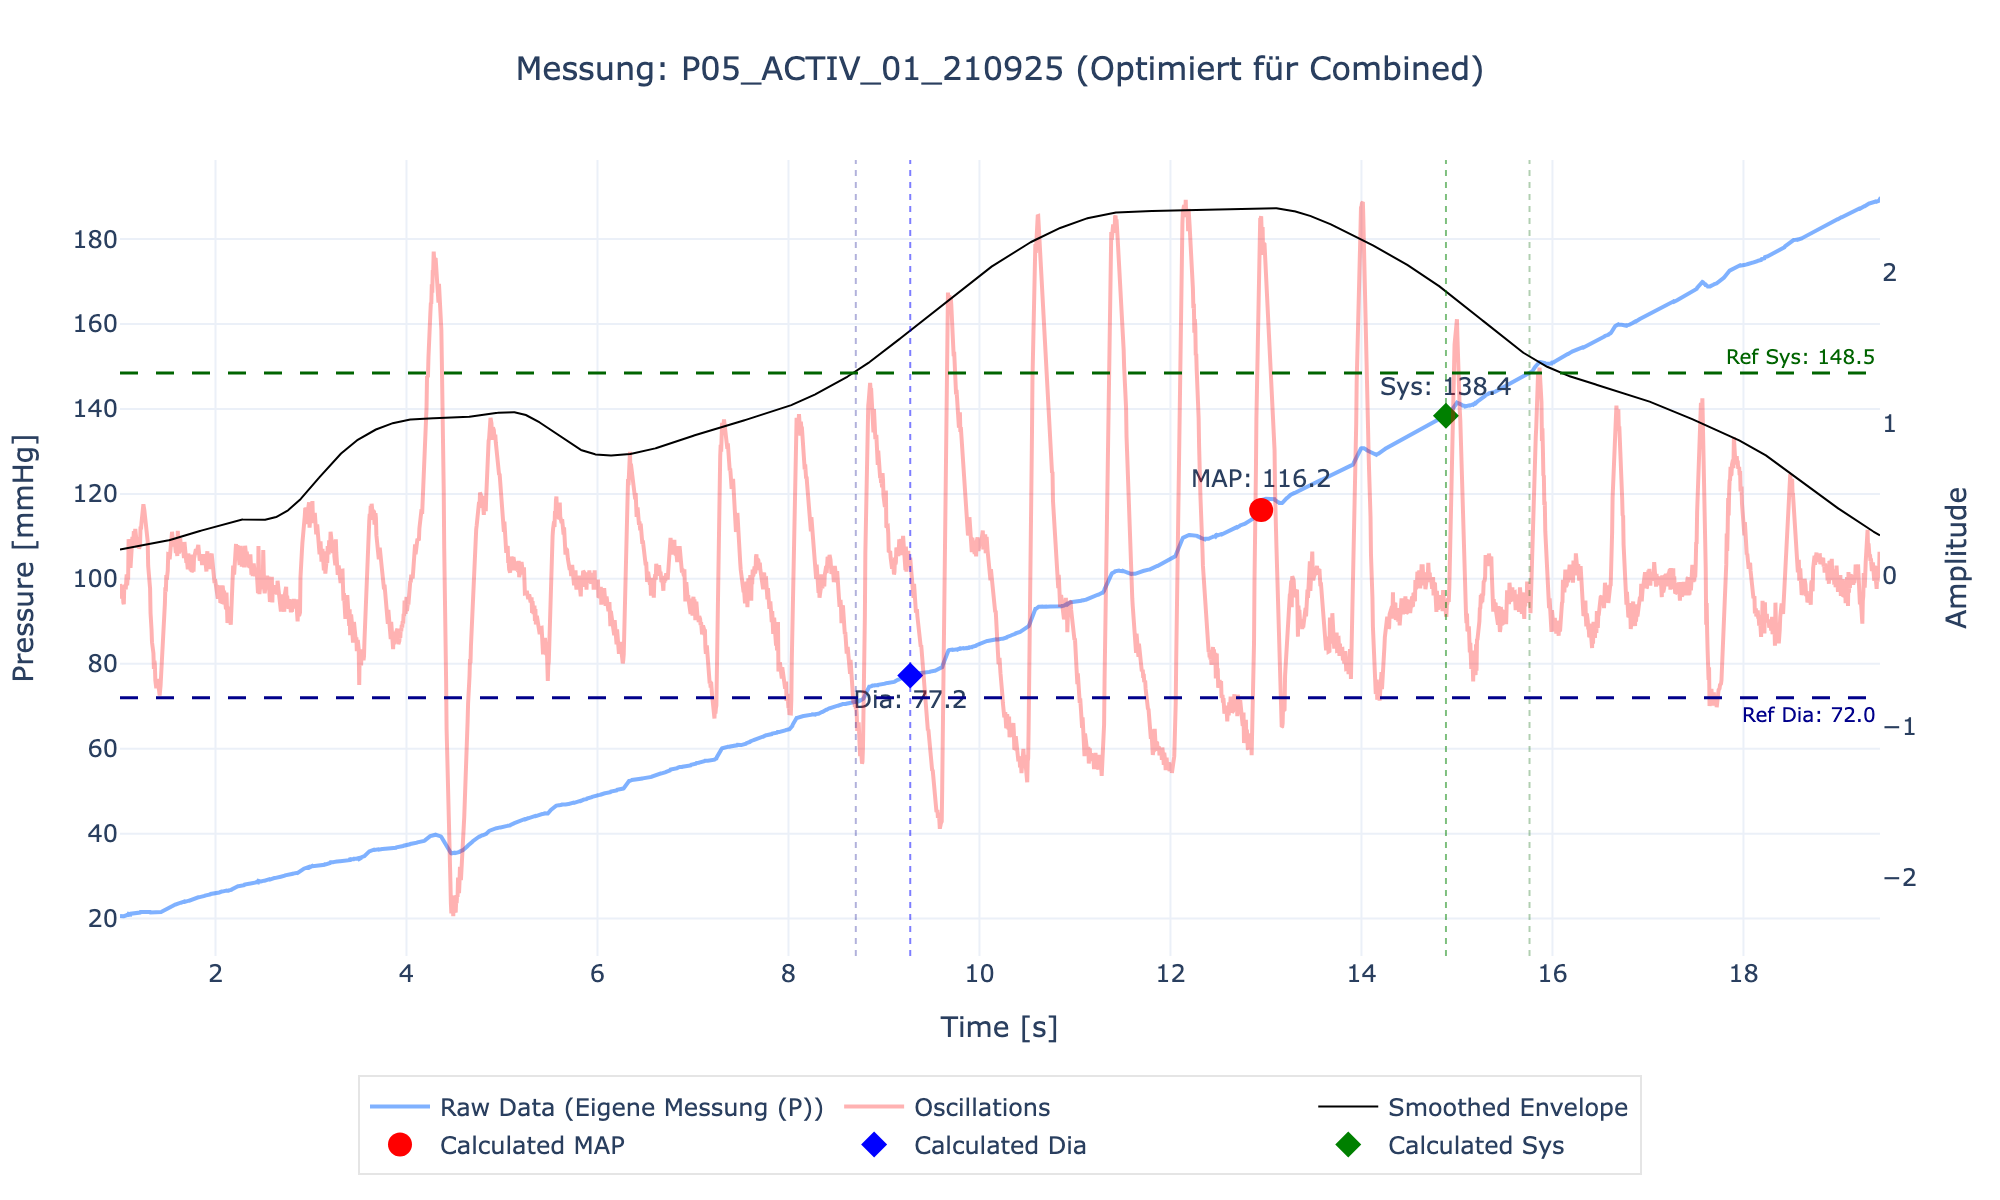
\includegraphics[width=\textwidth]{images/P05_ACTIV_01_210925_combined.png}
        \caption{Optimiert für Beurer und NAIS (Kombiniert)}
    \end{subfigure} \\
    \begin{subfigure}[b]{0.48\textwidth}
        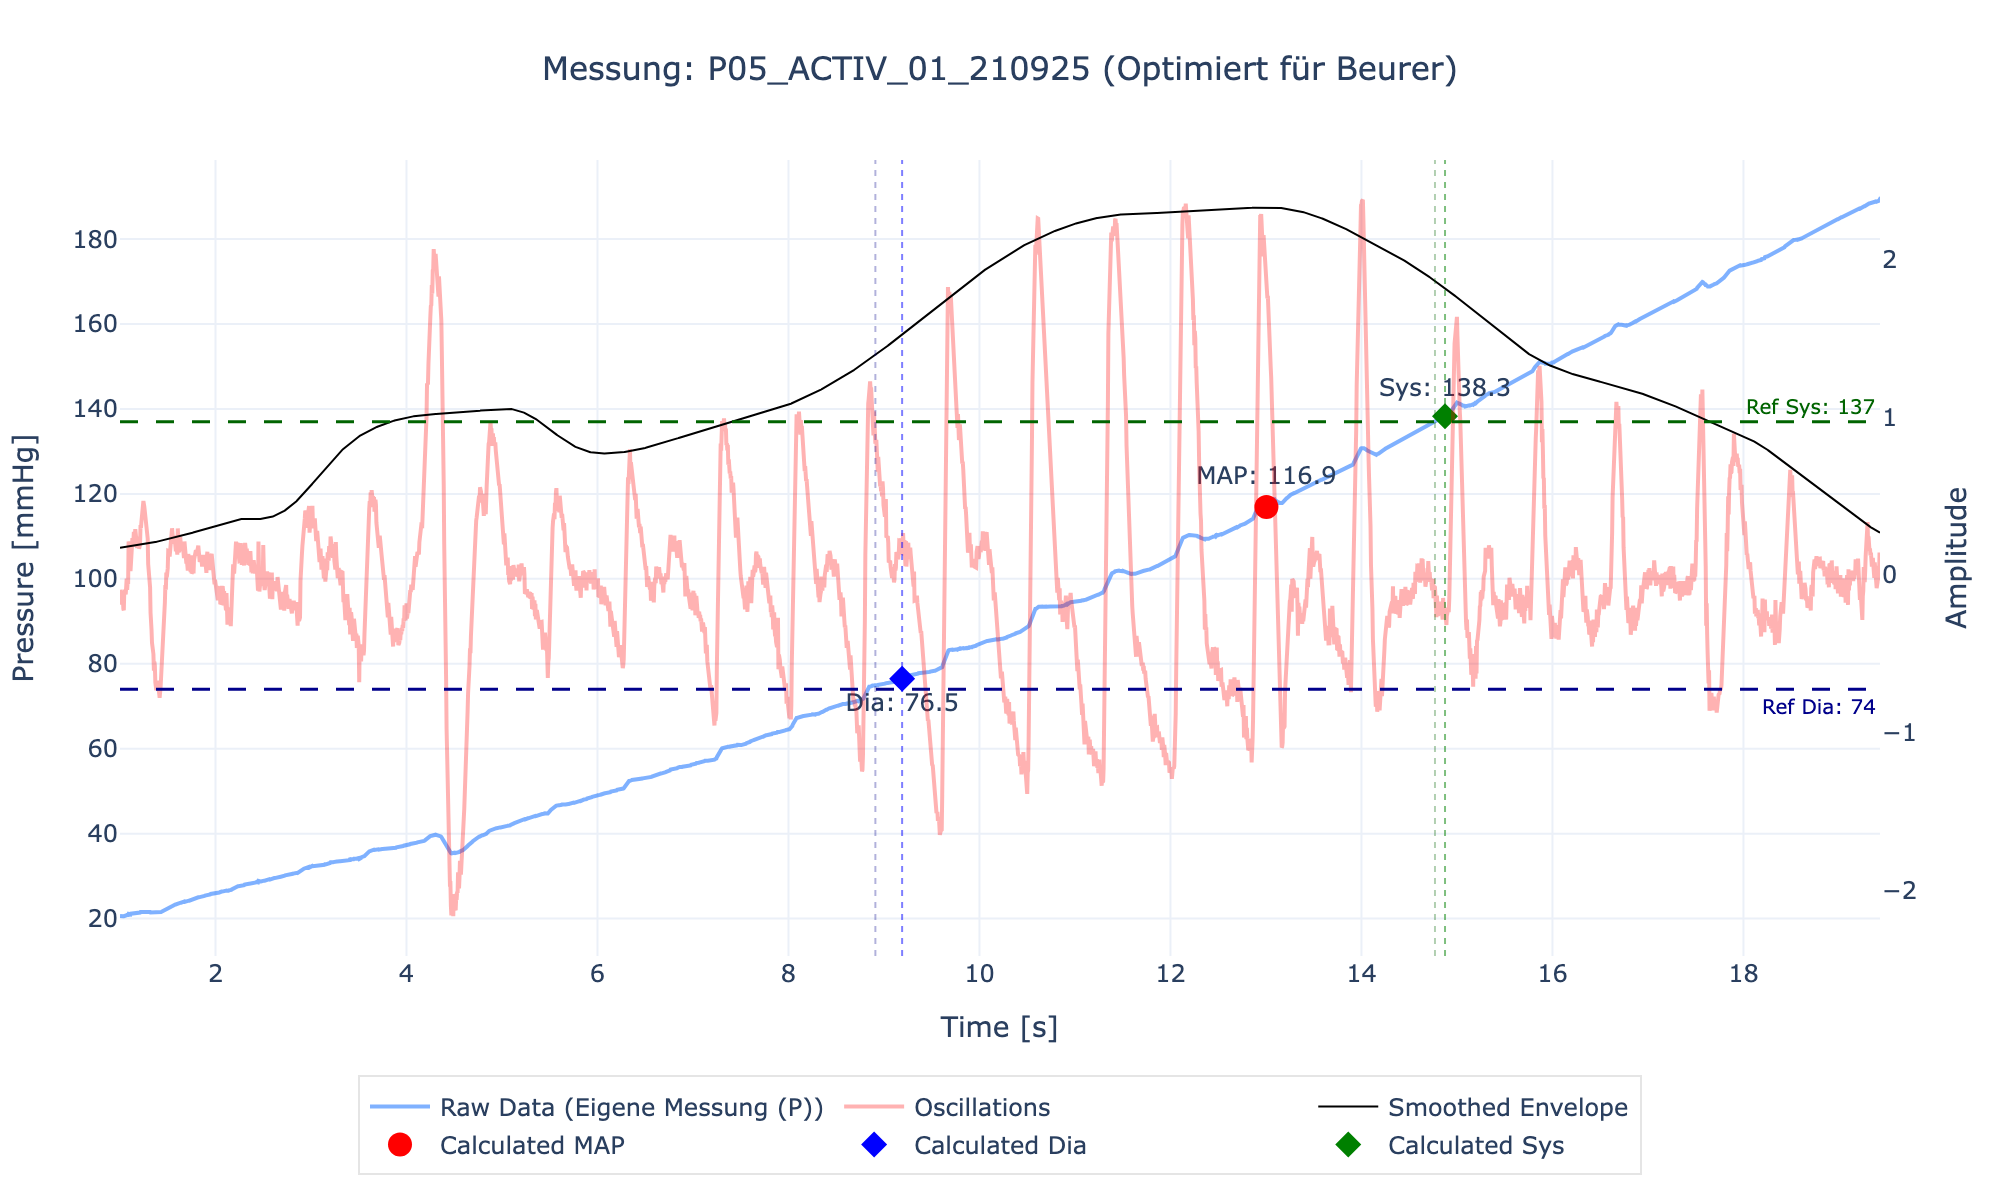
\includegraphics[width=\textwidth]{images/P05_ACTIV_01_210925_beurer.png}
        \caption{Optimiert für Beurer}
    \end{subfigure}
    \hfill
    \begin{subfigure}[b]{0.48\textwidth}
        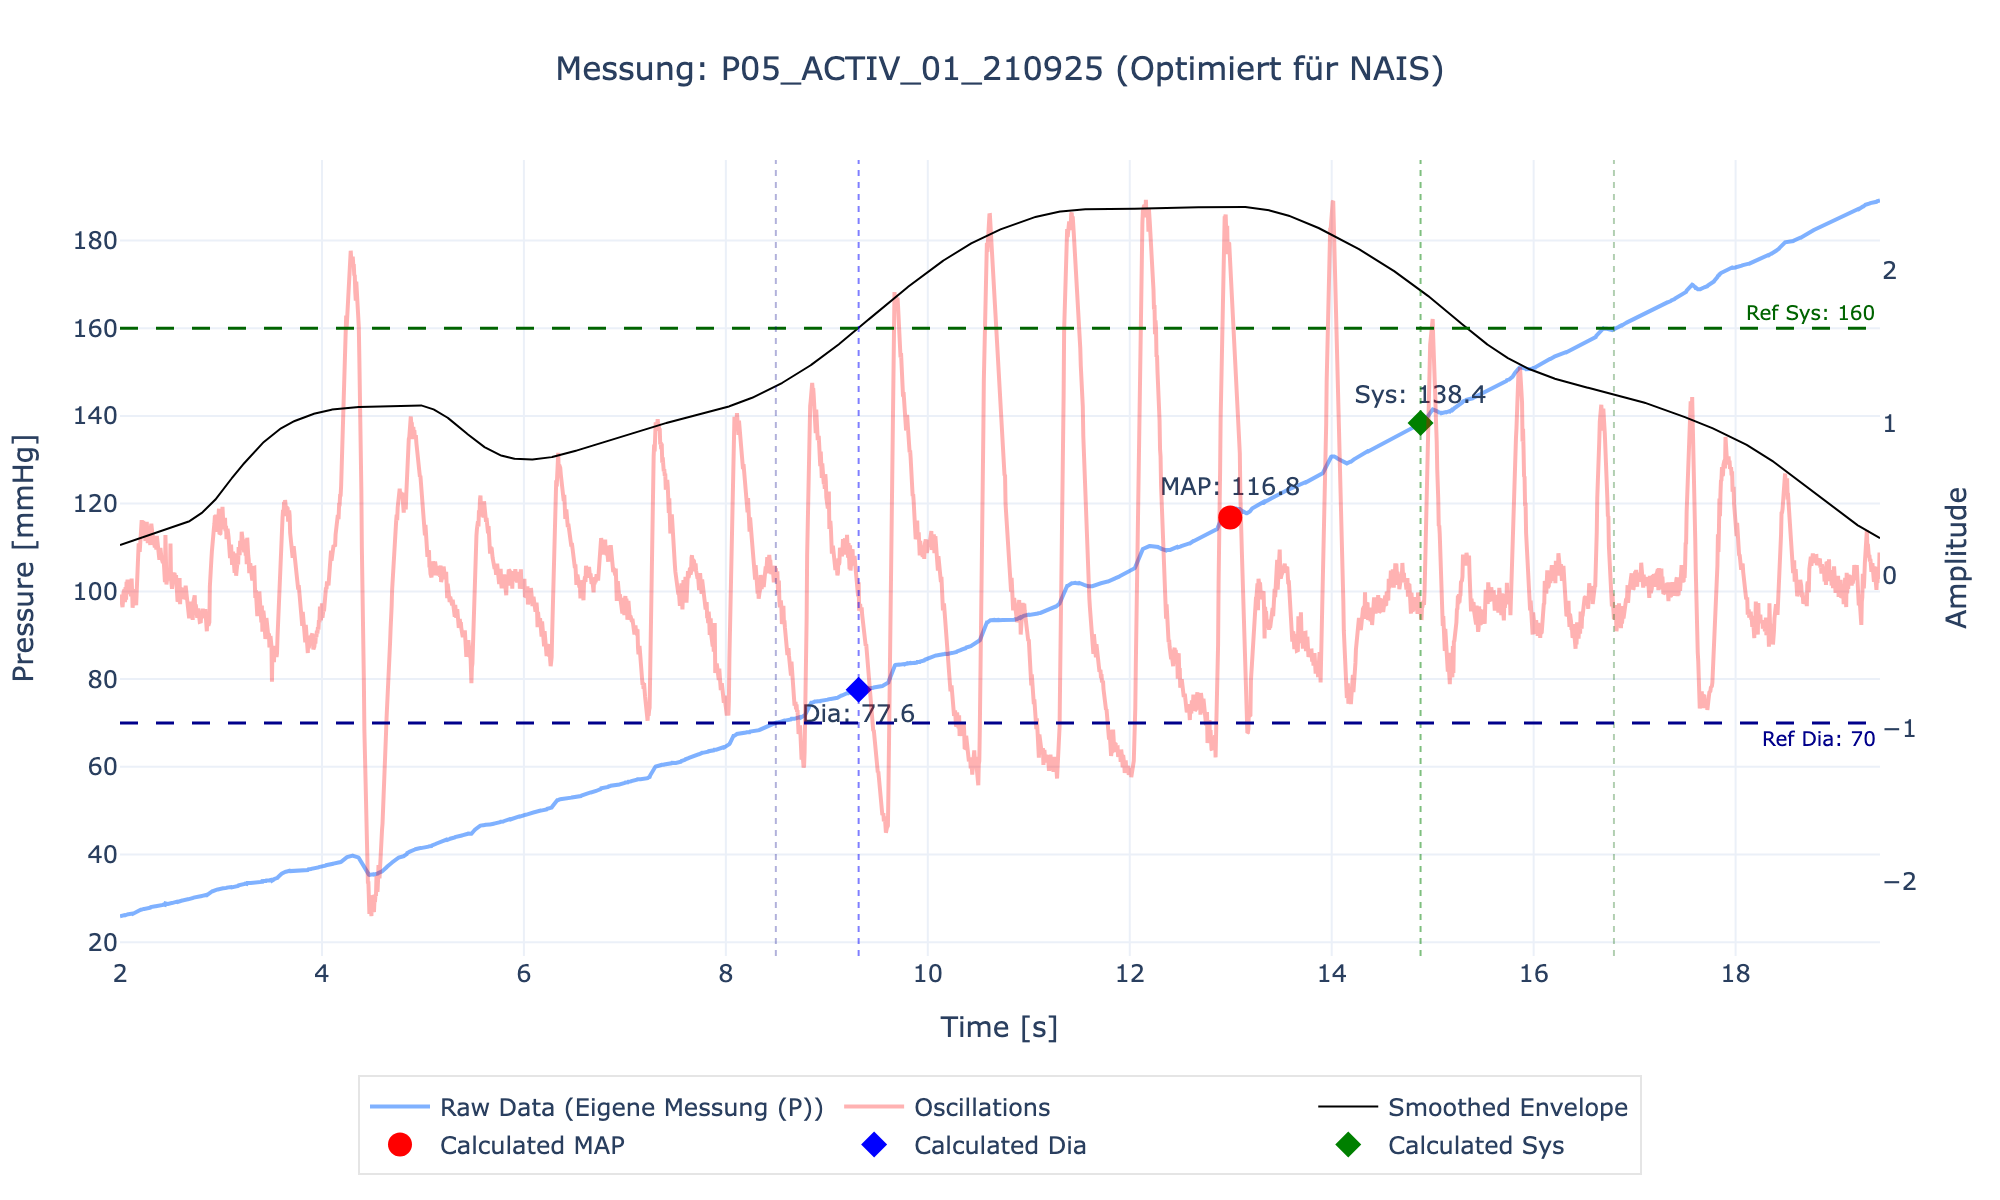
\includegraphics[width=\textwidth]{images/P05_ACTIV_01_210925_nais.png}
        \caption{Optimiert für NAIS}
    \end{subfigure}
    \caption{Einzelauswertung der Messung P05\_ACTIV\_01\_210925 mit verschiedenen Parametersätzen.}
\end{figure}
\newpage

\subsection*{Messung: P05\_REST\_01\_210925}
\begin{figure}[H]
    \centering
    \begin{subfigure}[b]{0.8\textwidth}
        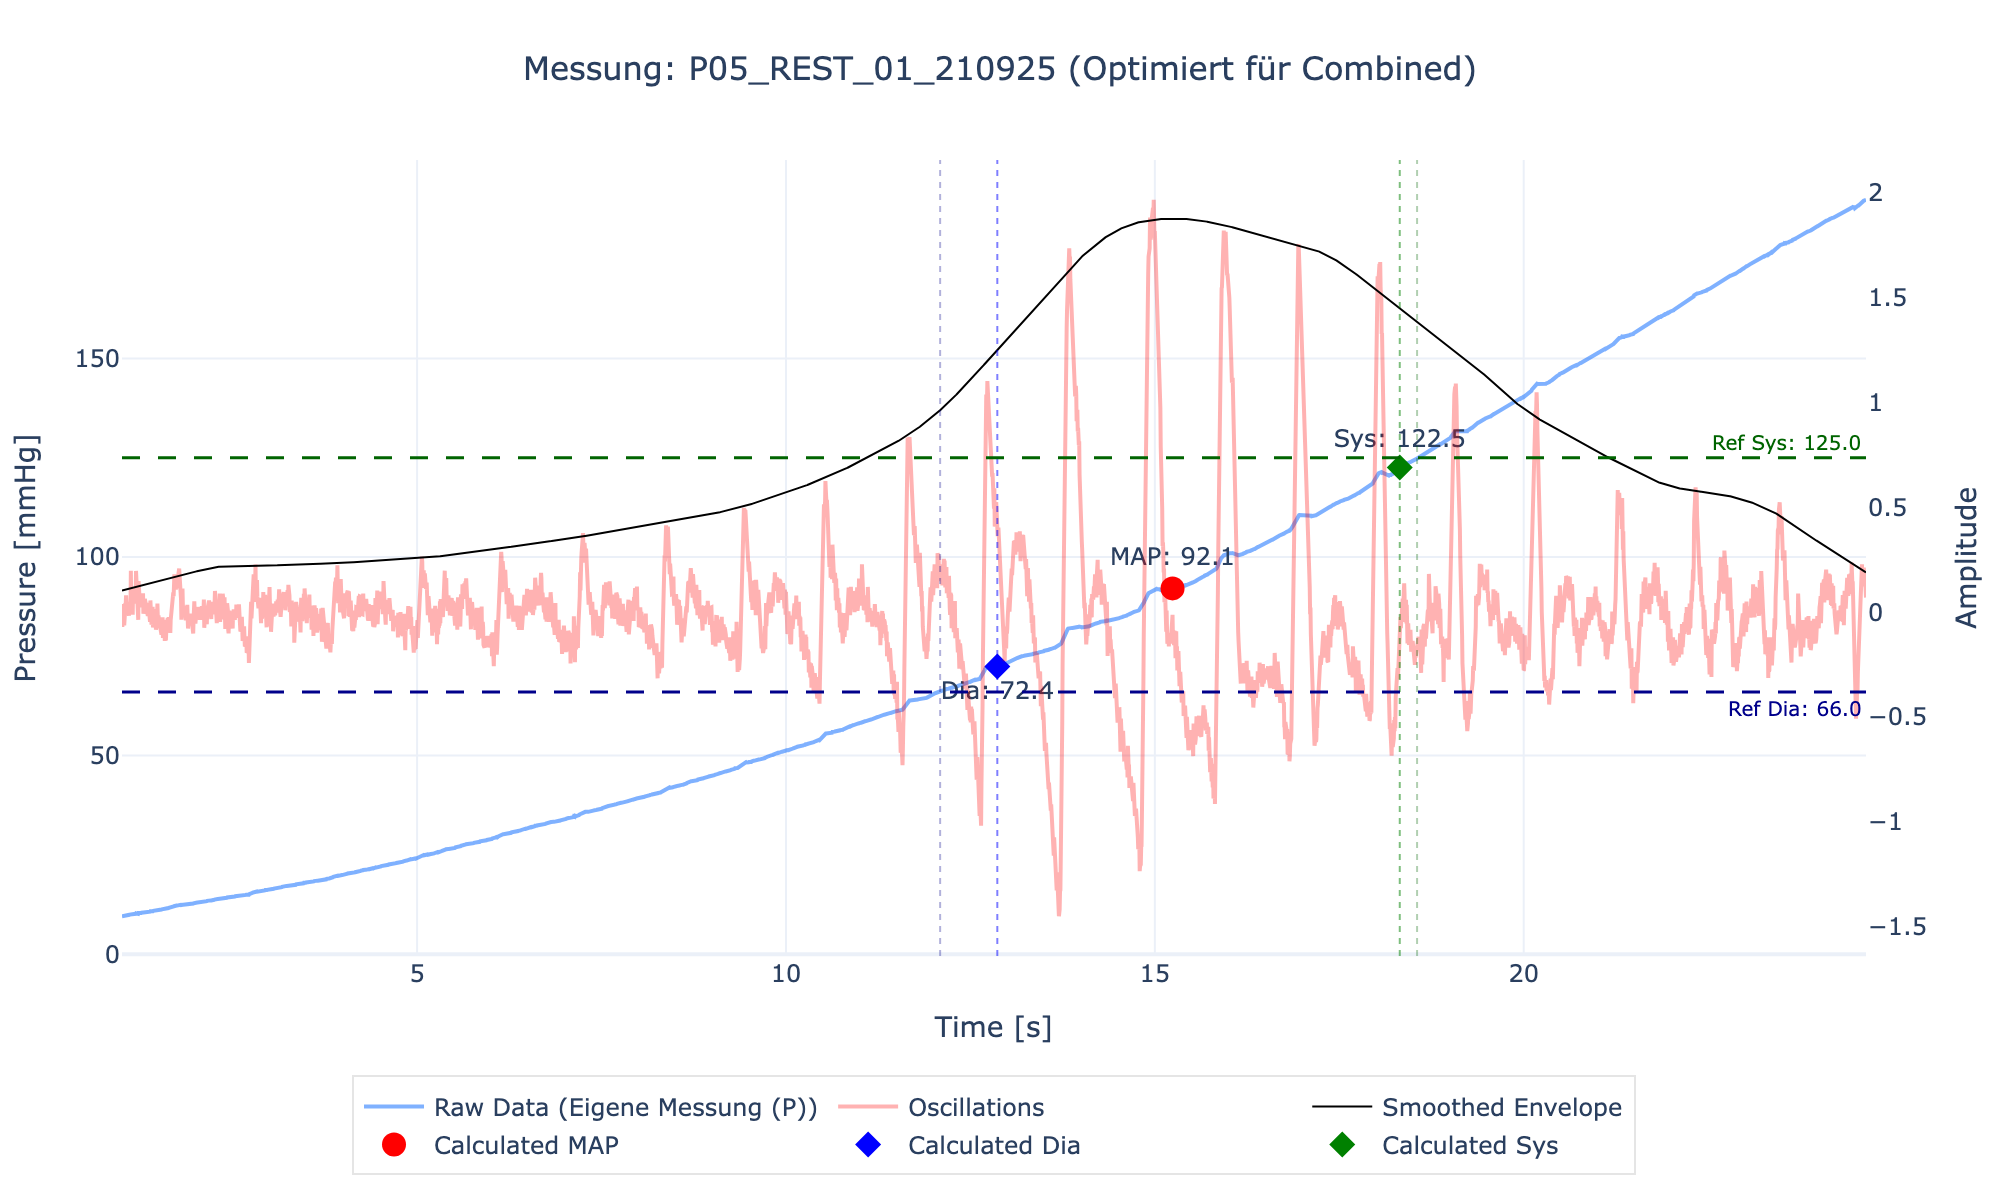
\includegraphics[width=\textwidth]{images/P05_REST_01_210925_combined.png}
        \caption{Optimiert für Beurer und NAIS (Kombiniert)}
    \end{subfigure} \\
    \begin{subfigure}[b]{0.48\textwidth}
        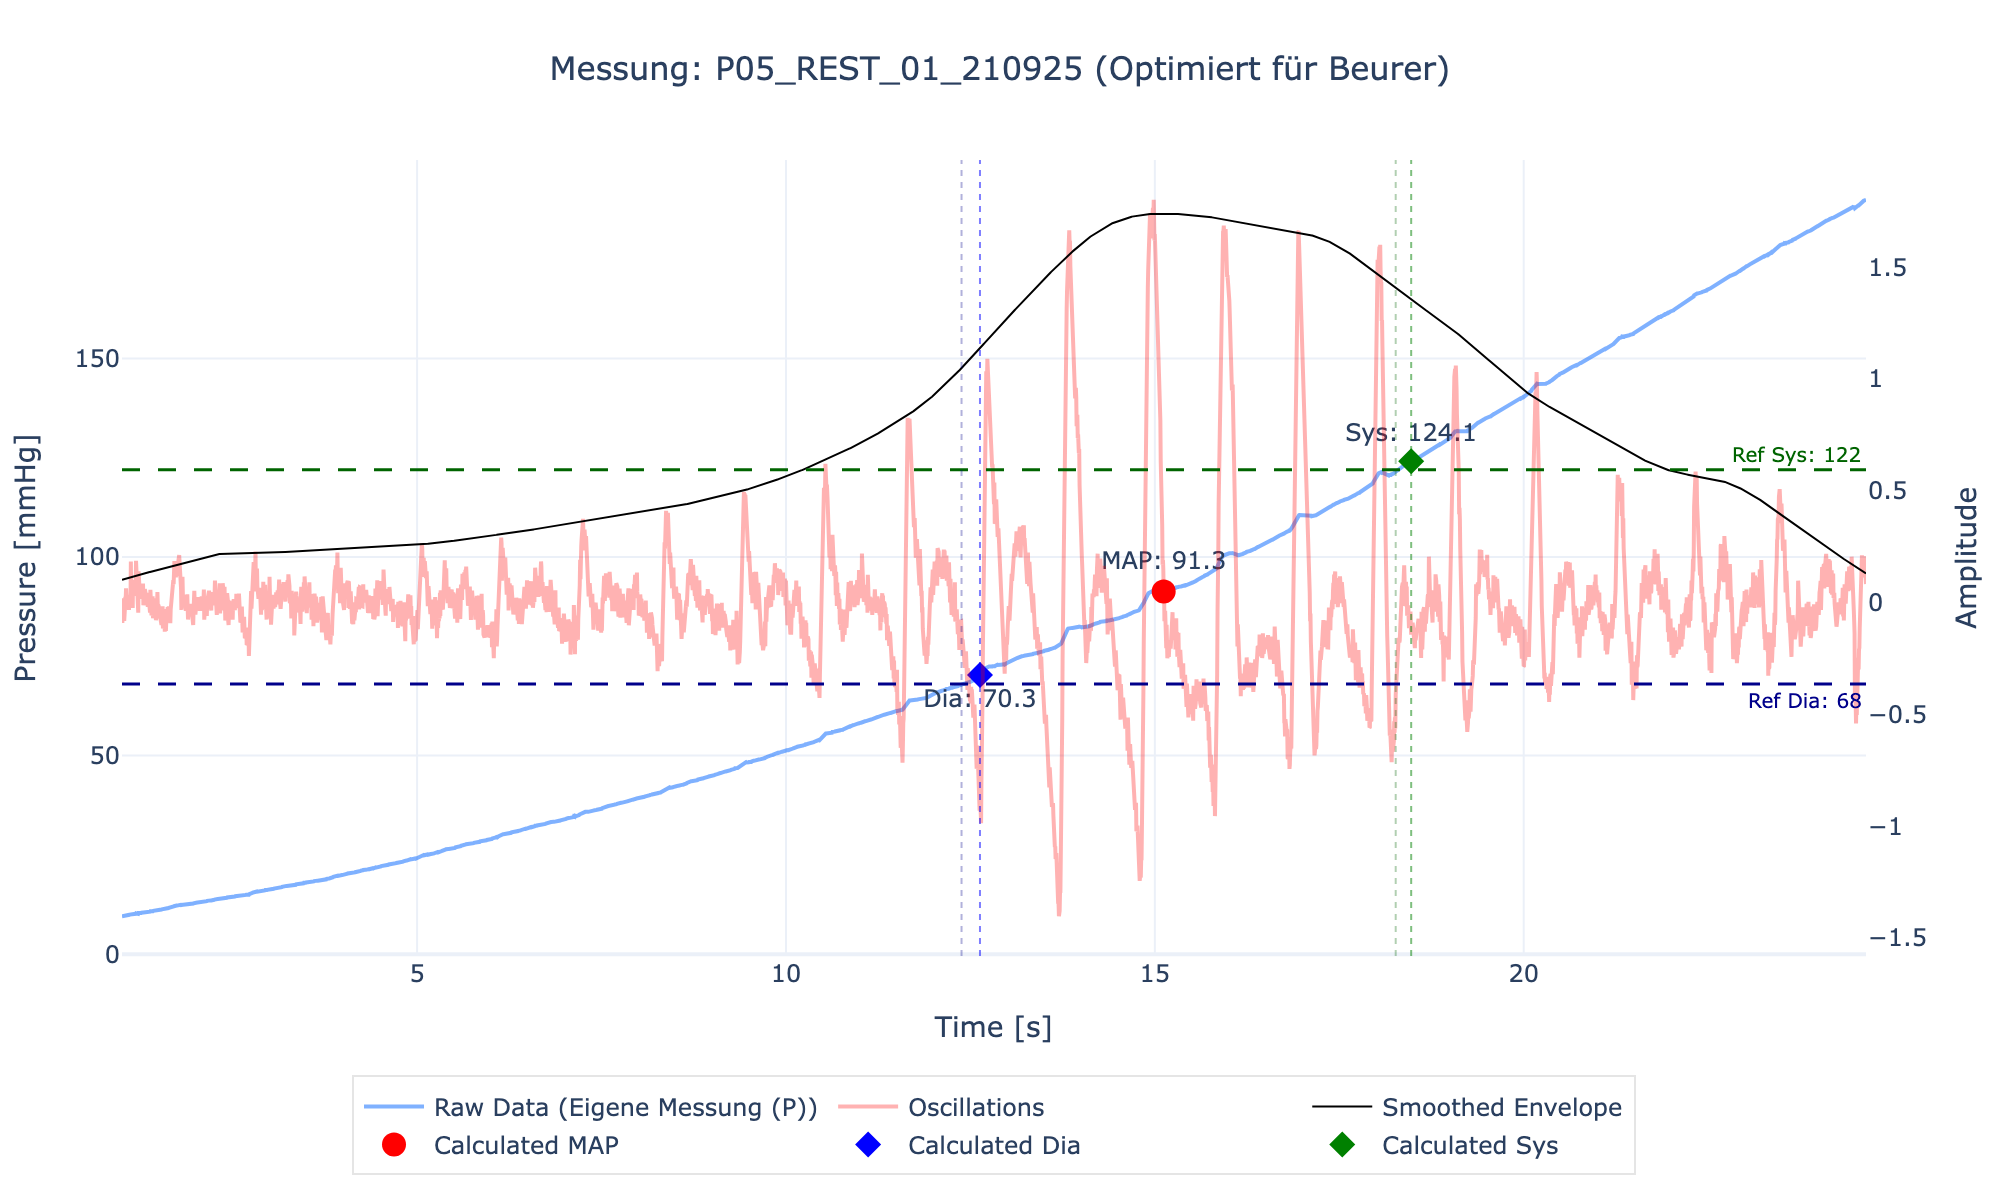
\includegraphics[width=\textwidth]{images/P05_REST_01_210925_beurer.png}
        \caption{Optimiert für Beurer}
    \end{subfigure}
    \hfill
    \begin{subfigure}[b]{0.48\textwidth}
        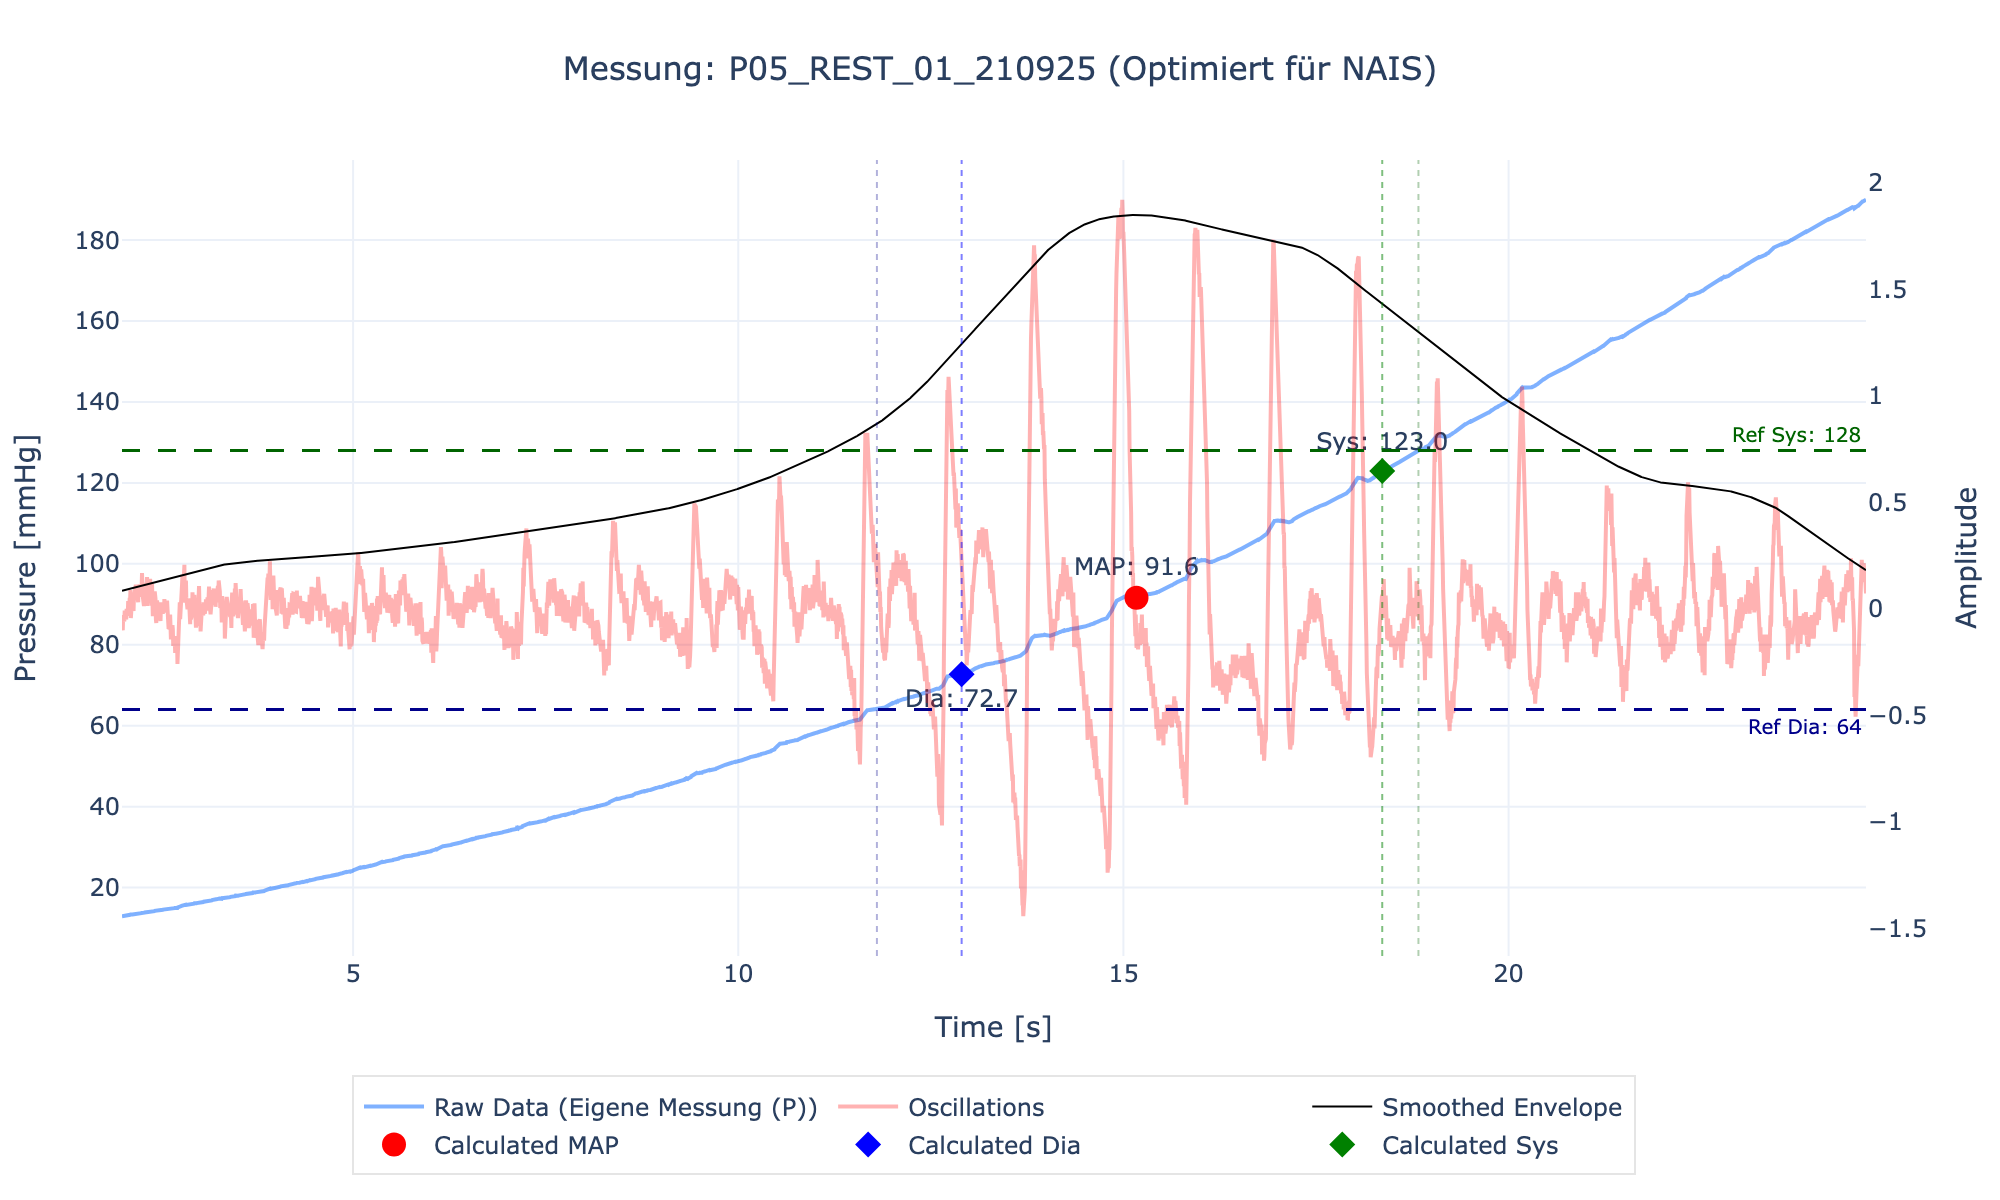
\includegraphics[width=\textwidth]{images/P05_REST_01_210925_nais.png}
        \caption{Optimiert für NAIS}
    \end{subfigure}
    \caption{Einzelauswertung der Messung P05\_REST\_01\_210925 mit verschiedenen Parametersätzen.}
\end{figure}
\newpage

\subsection*{Messung: P06\_ACTIV\_01\_191025}
\begin{figure}[H]
    \centering
    \begin{subfigure}[b]{0.8\textwidth}
        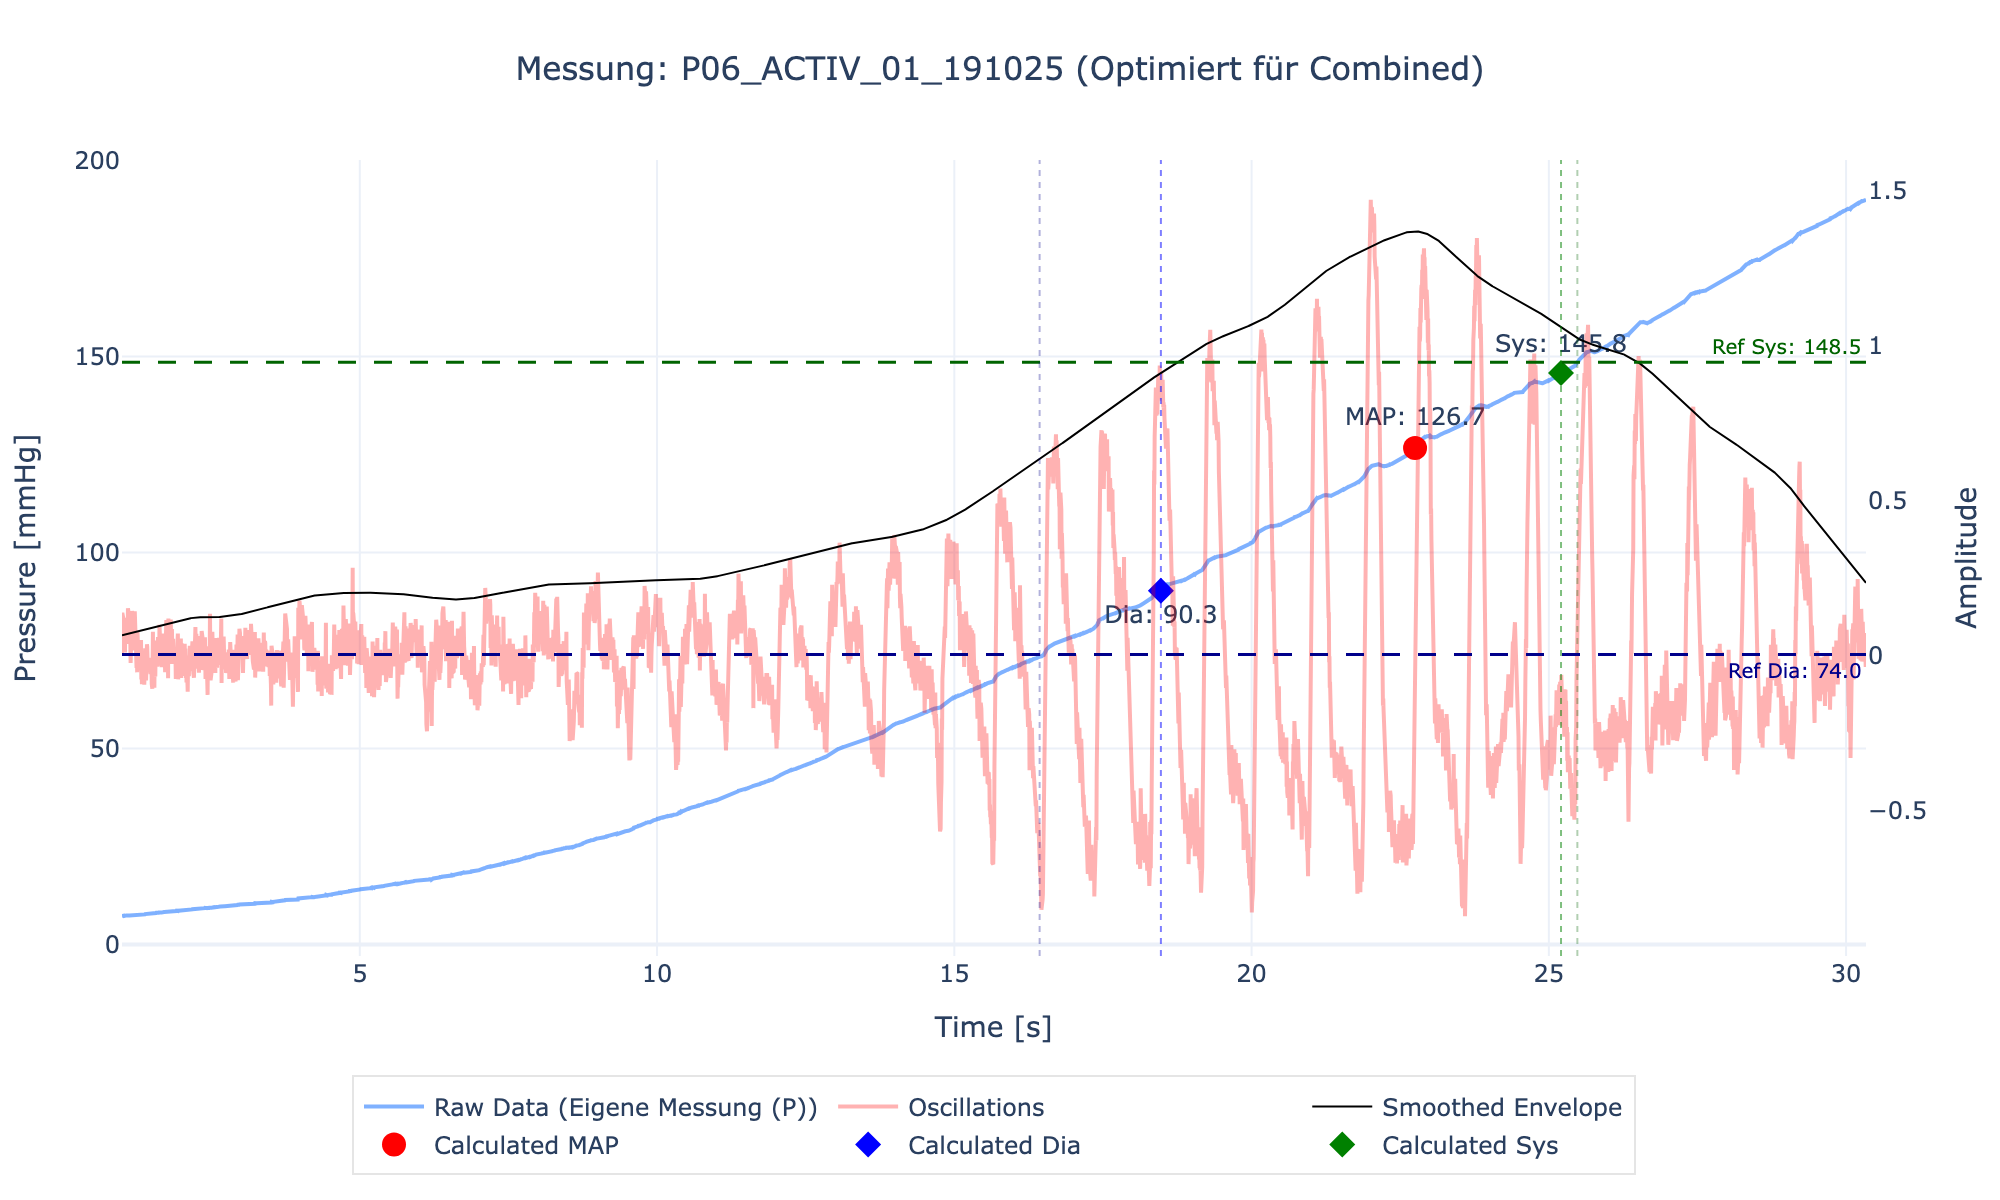
\includegraphics[width=\textwidth]{images/P06_ACTIV_01_191025_combined.png}
        \caption{Optimiert für Beurer und NAIS (Kombiniert)}
    \end{subfigure} \\
    \begin{subfigure}[b]{0.48\textwidth}
        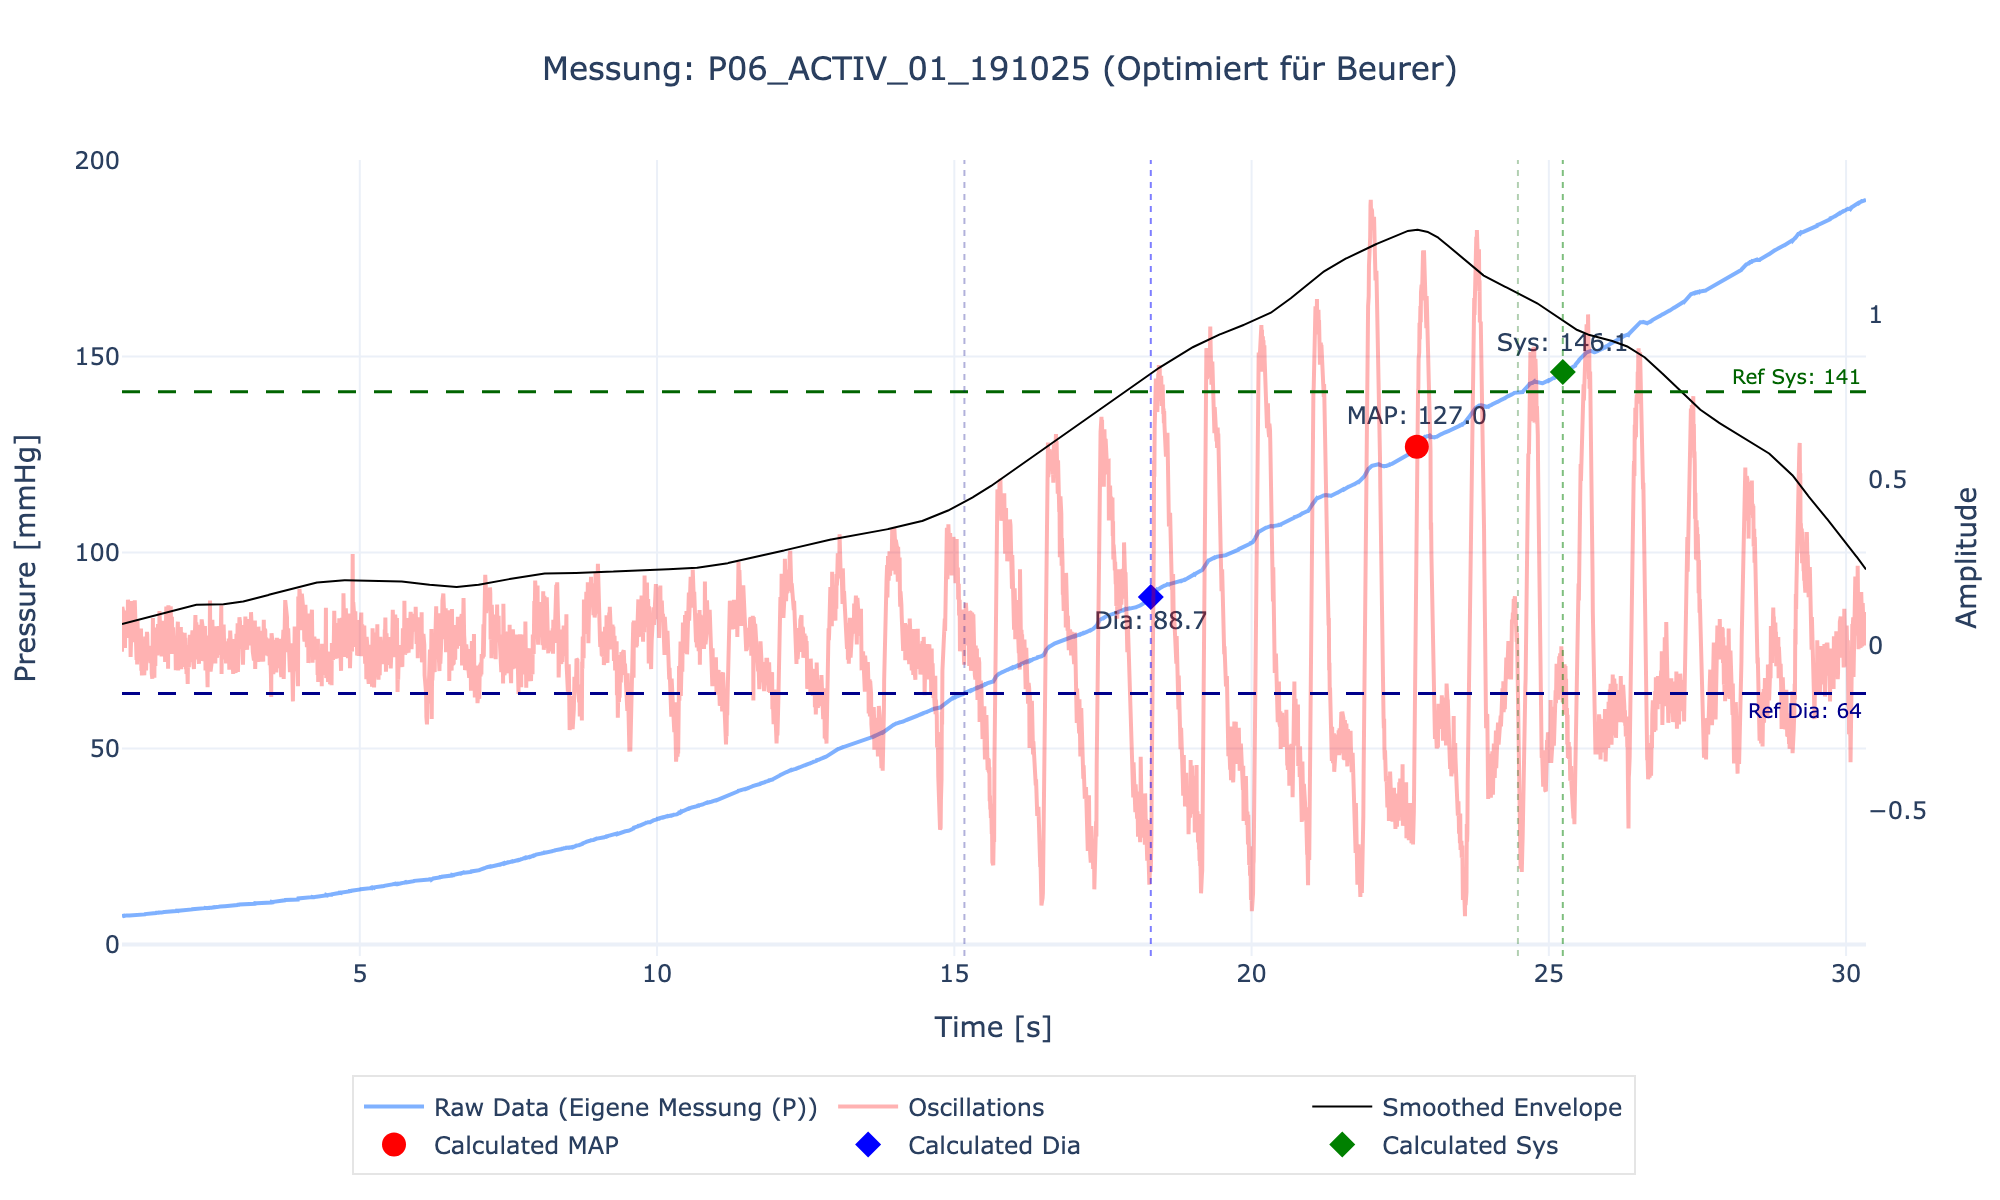
\includegraphics[width=\textwidth]{images/P06_ACTIV_01_191025_beurer.png}
        \caption{Optimiert für Beurer}
    \end{subfigure}
    \hfill
    \begin{subfigure}[b]{0.48\textwidth}
        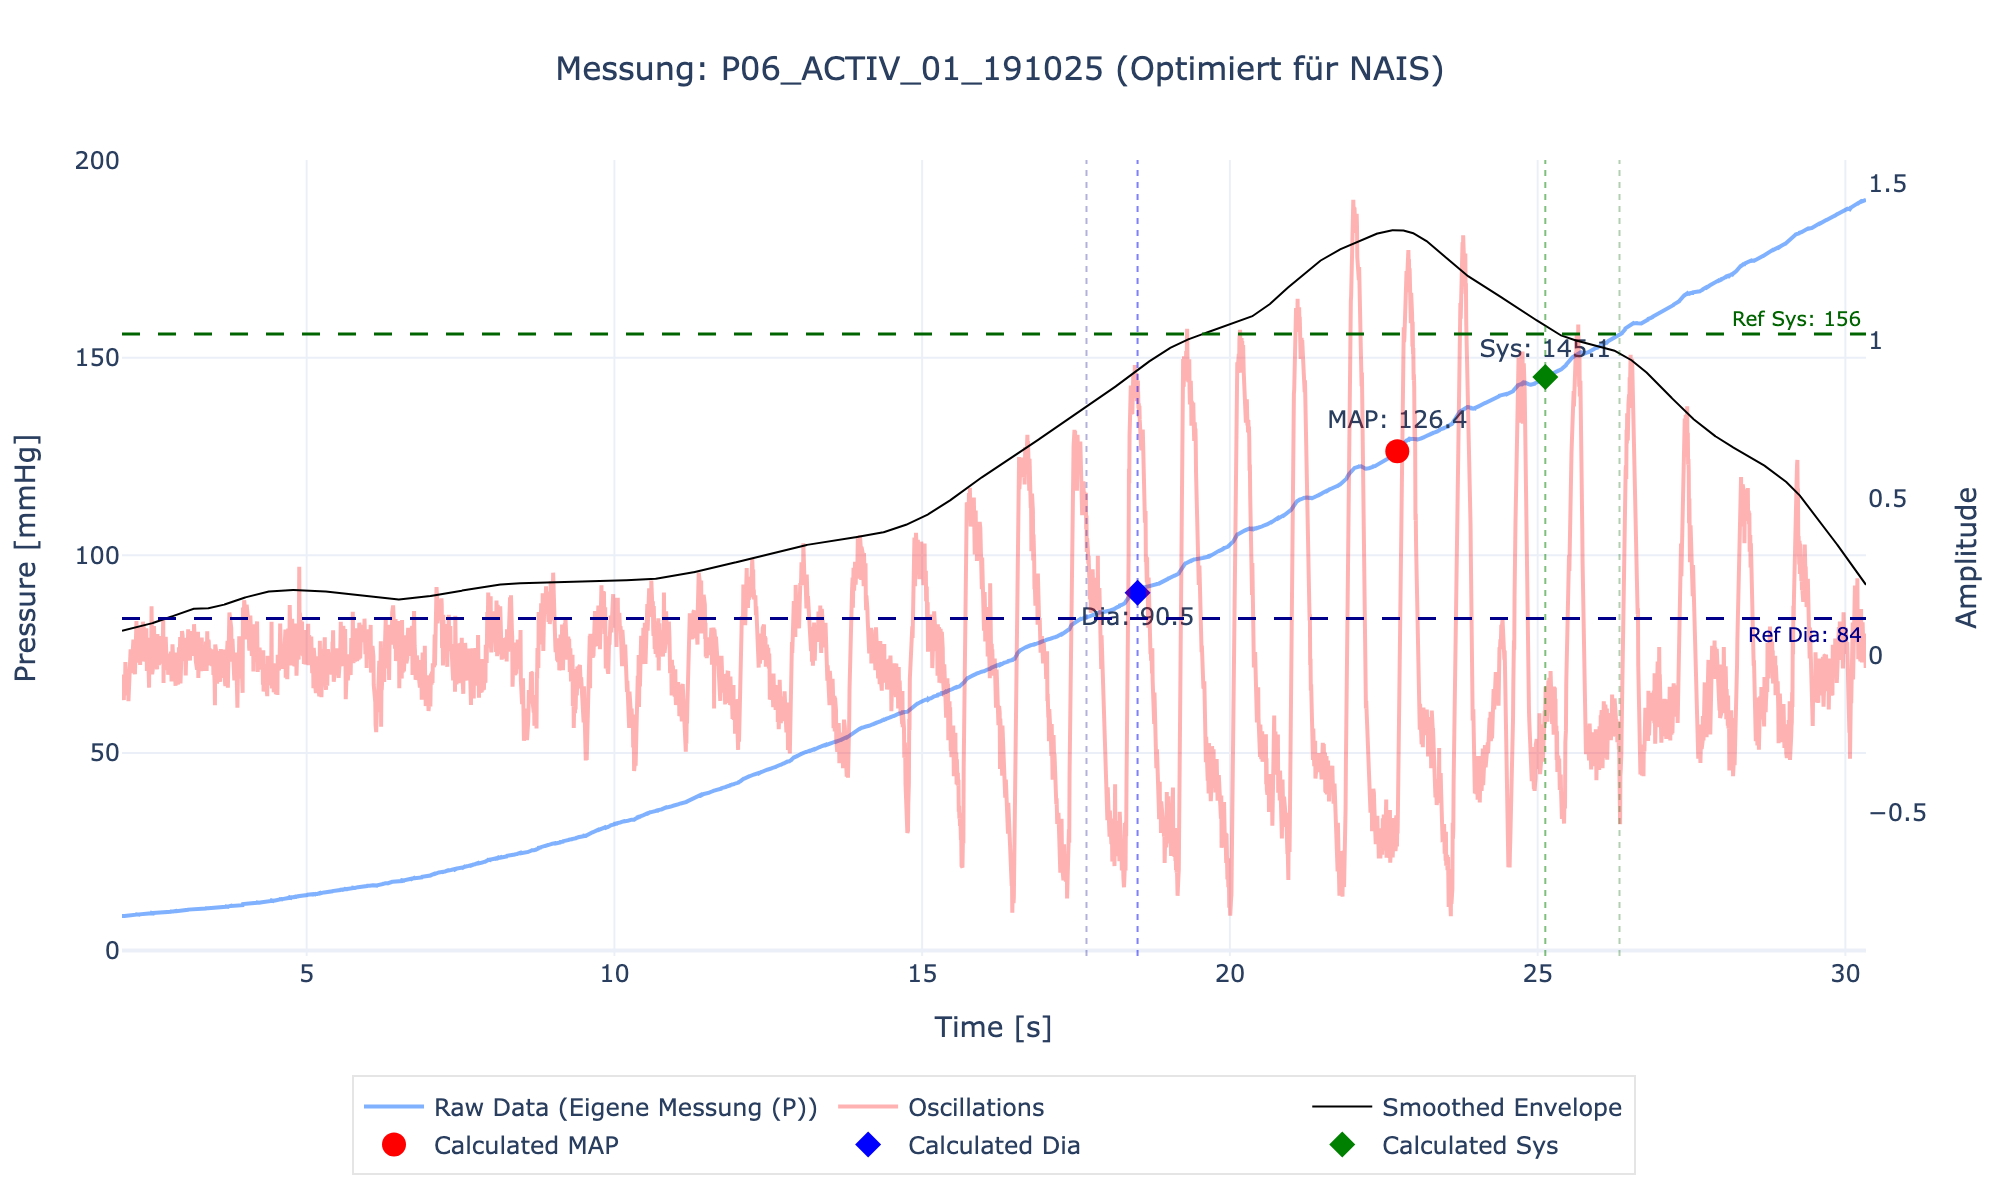
\includegraphics[width=\textwidth]{images/P06_ACTIV_01_191025_nais.png}
        \caption{Optimiert für NAIS}
    \end{subfigure}
    \caption{Einzelauswertung der Messung P06\_ACTIV\_01\_191025 mit verschiedenen Parametersätzen.}
\end{figure}
\newpage

\subsection*{Messung: P06\_REST\_01\_191025}
\begin{figure}[H]
    \centering
    \begin{subfigure}[b]{0.8\textwidth}
        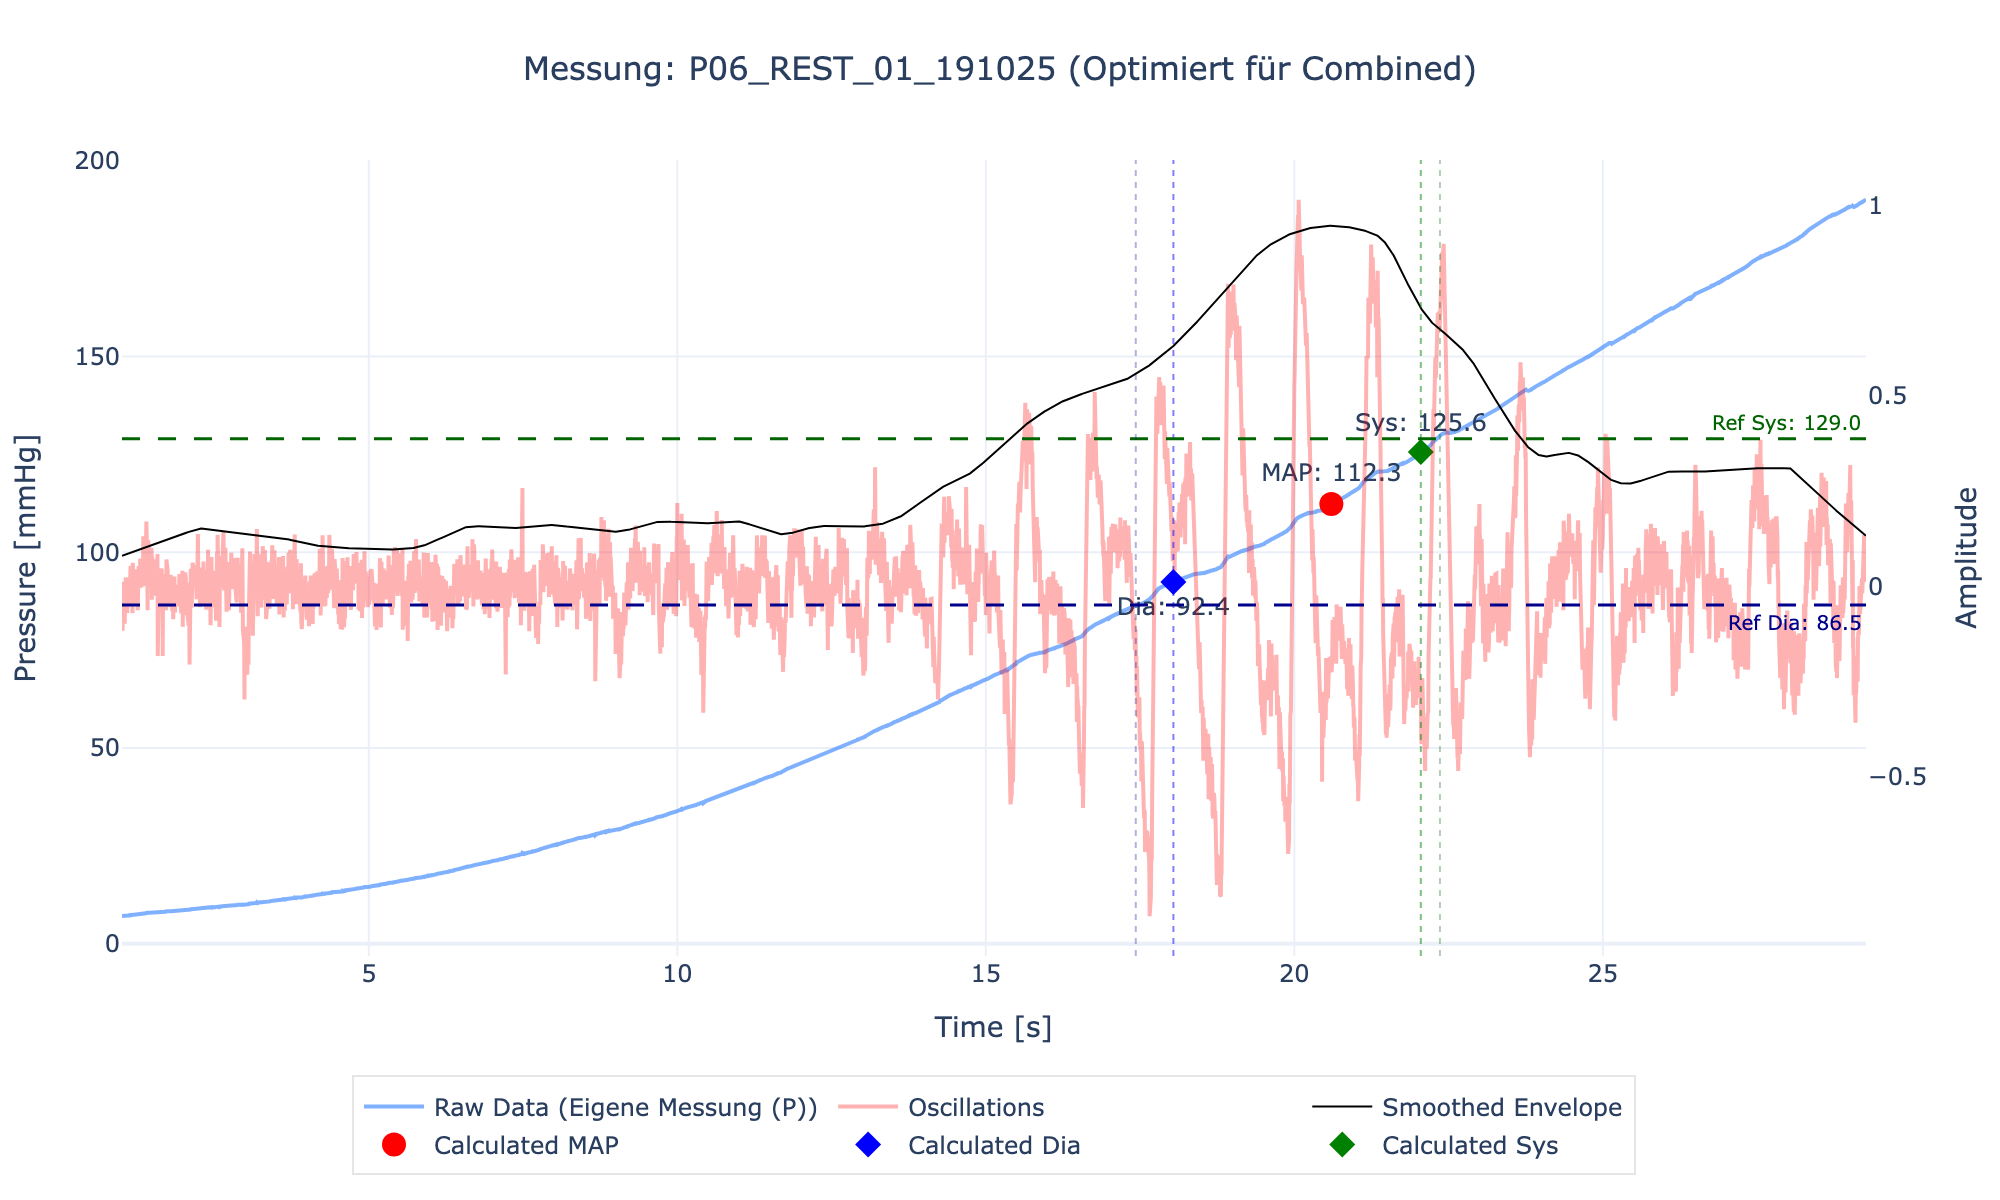
\includegraphics[width=\textwidth]{images/P06_REST_01_191025_combined.png}
        \caption{Optimiert für Beurer und NAIS (Kombiniert)}
    \end{subfigure} \\
    \begin{subfigure}[b]{0.48\textwidth}
        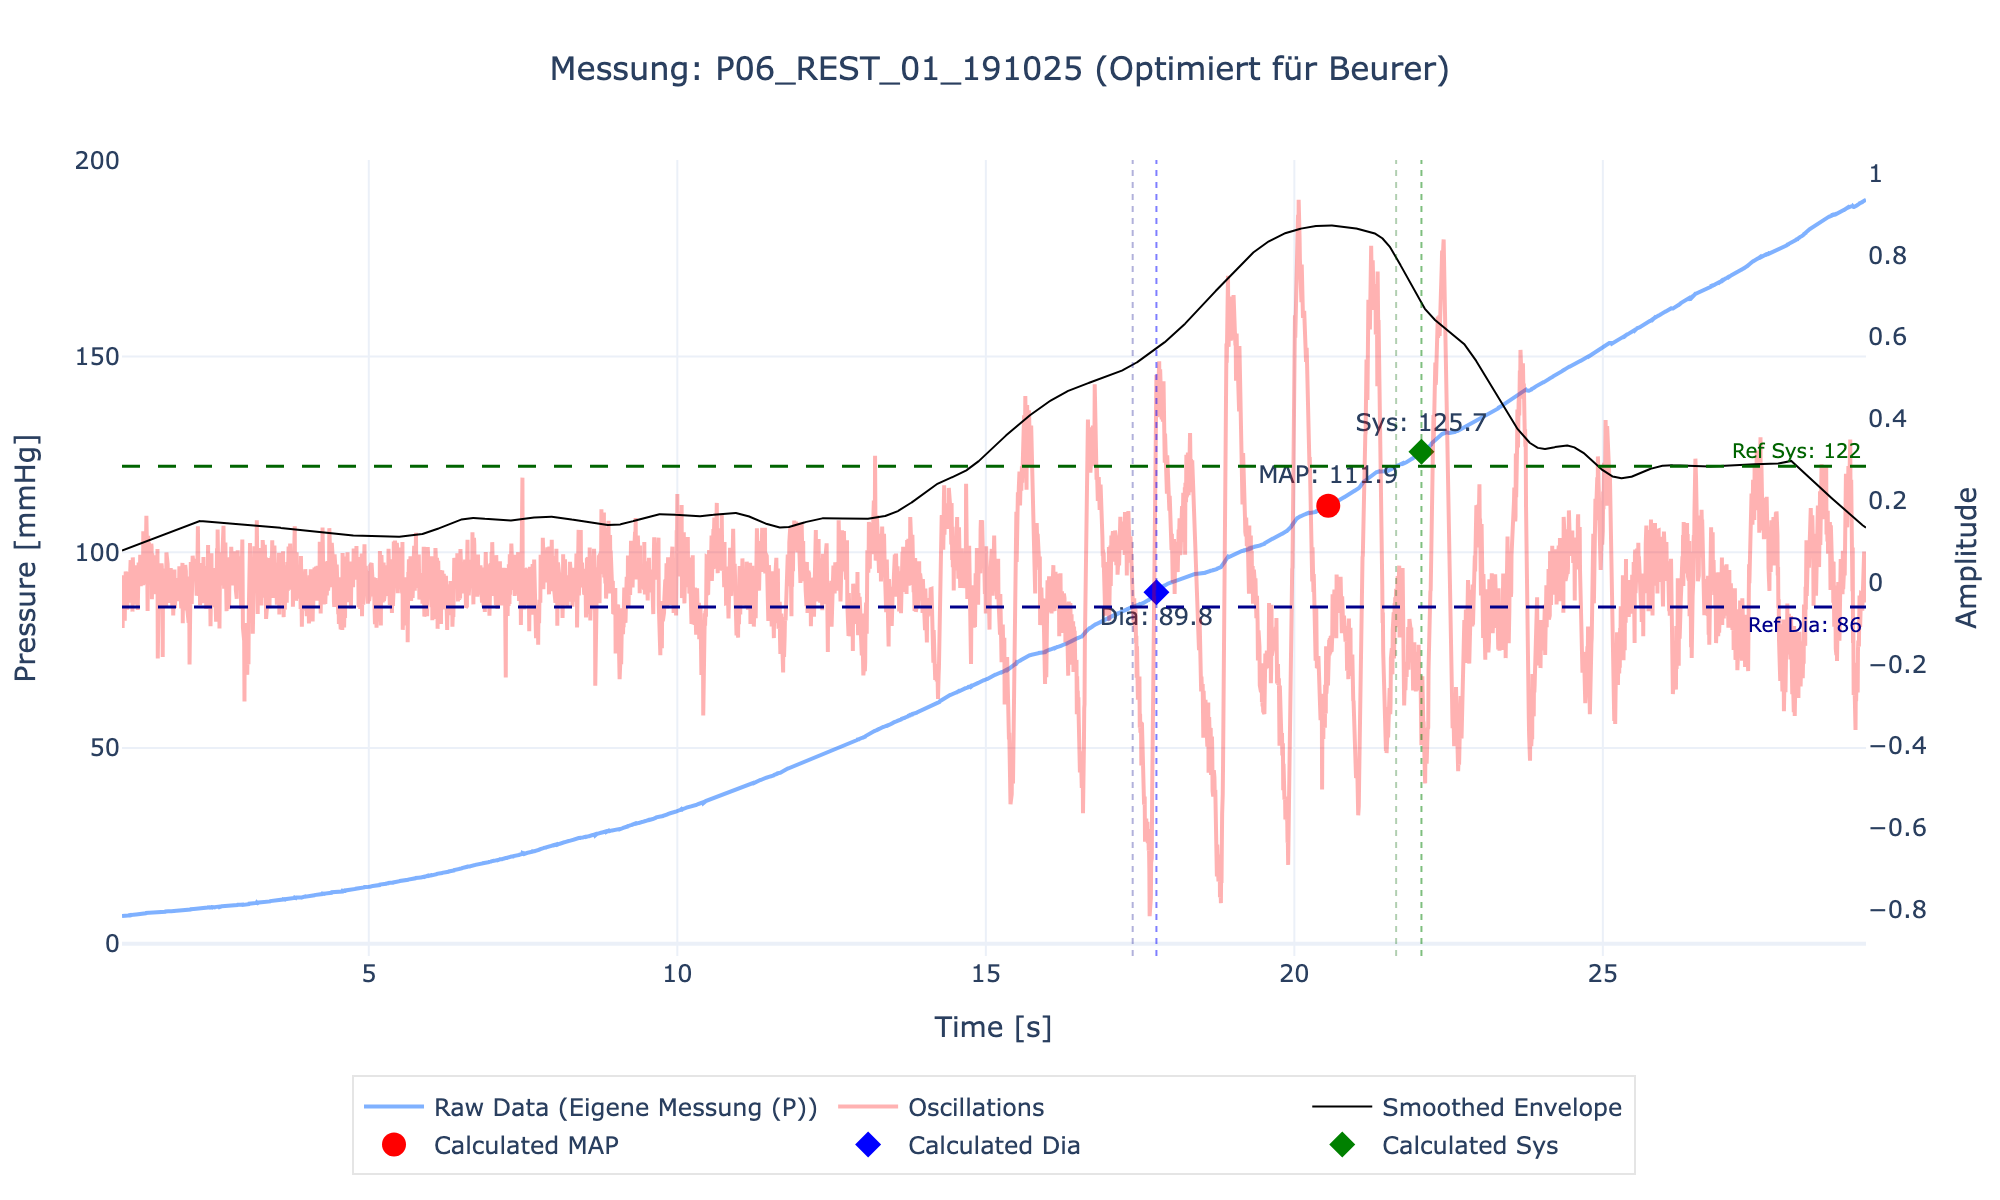
\includegraphics[width=\textwidth]{images/P06_REST_01_191025_beurer.png}
        \caption{Optimiert für Beurer}
    \end{subfigure}
    \hfill
    \begin{subfigure}[b]{0.48\textwidth}
        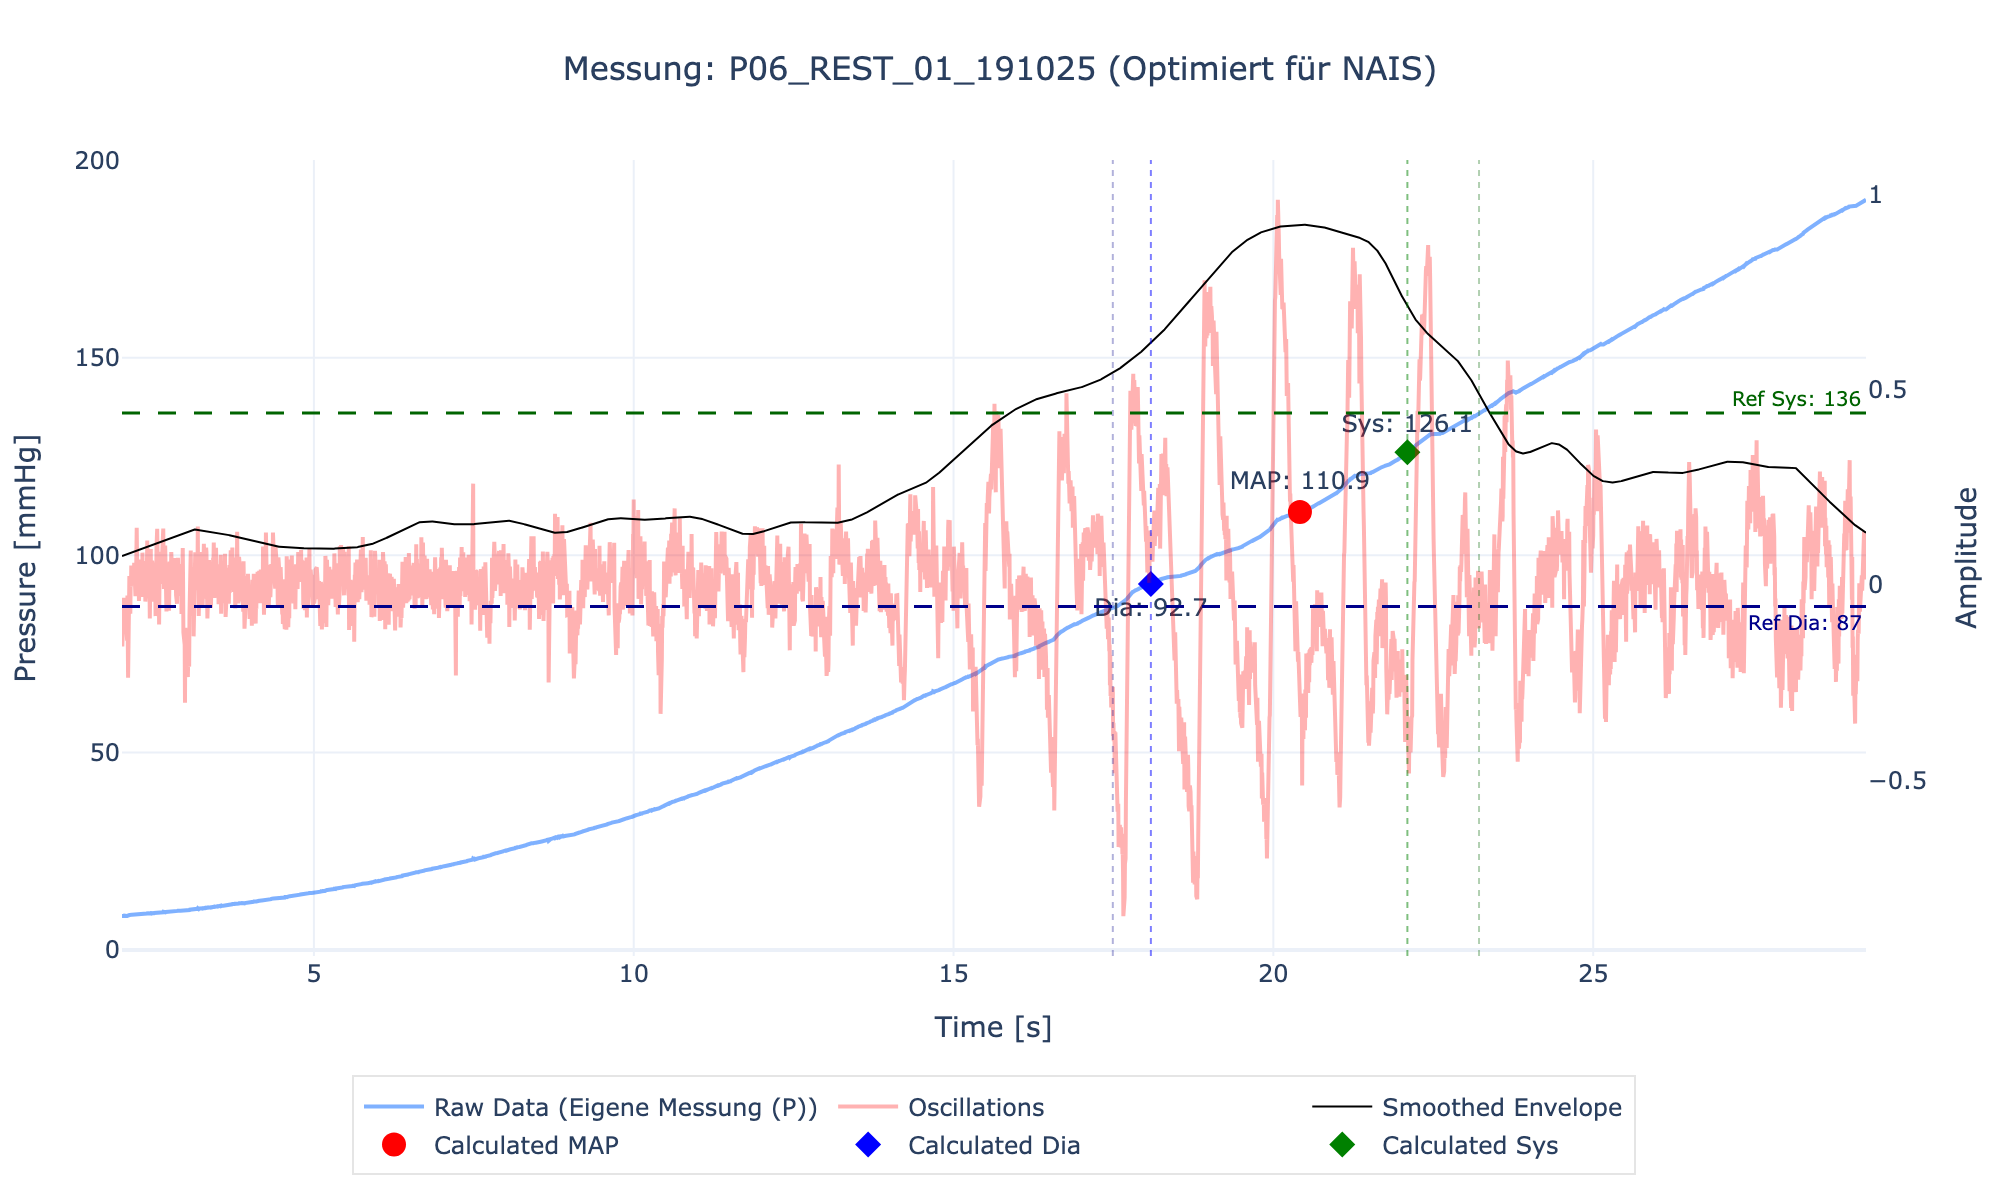
\includegraphics[width=\textwidth]{images/P06_REST_01_191025_nais.png}
        \caption{Optimiert für NAIS}
    \end{subfigure}
    \caption{Einzelauswertung der Messung P06\_REST\_01\_191025 mit verschiedenen Parametersätzen.}
\end{figure}
\newpage

\subsection*{Messung: P07\_ACTIV\_01\_191025}
\begin{figure}[H]
    \centering
    \begin{subfigure}[b]{0.8\textwidth}
        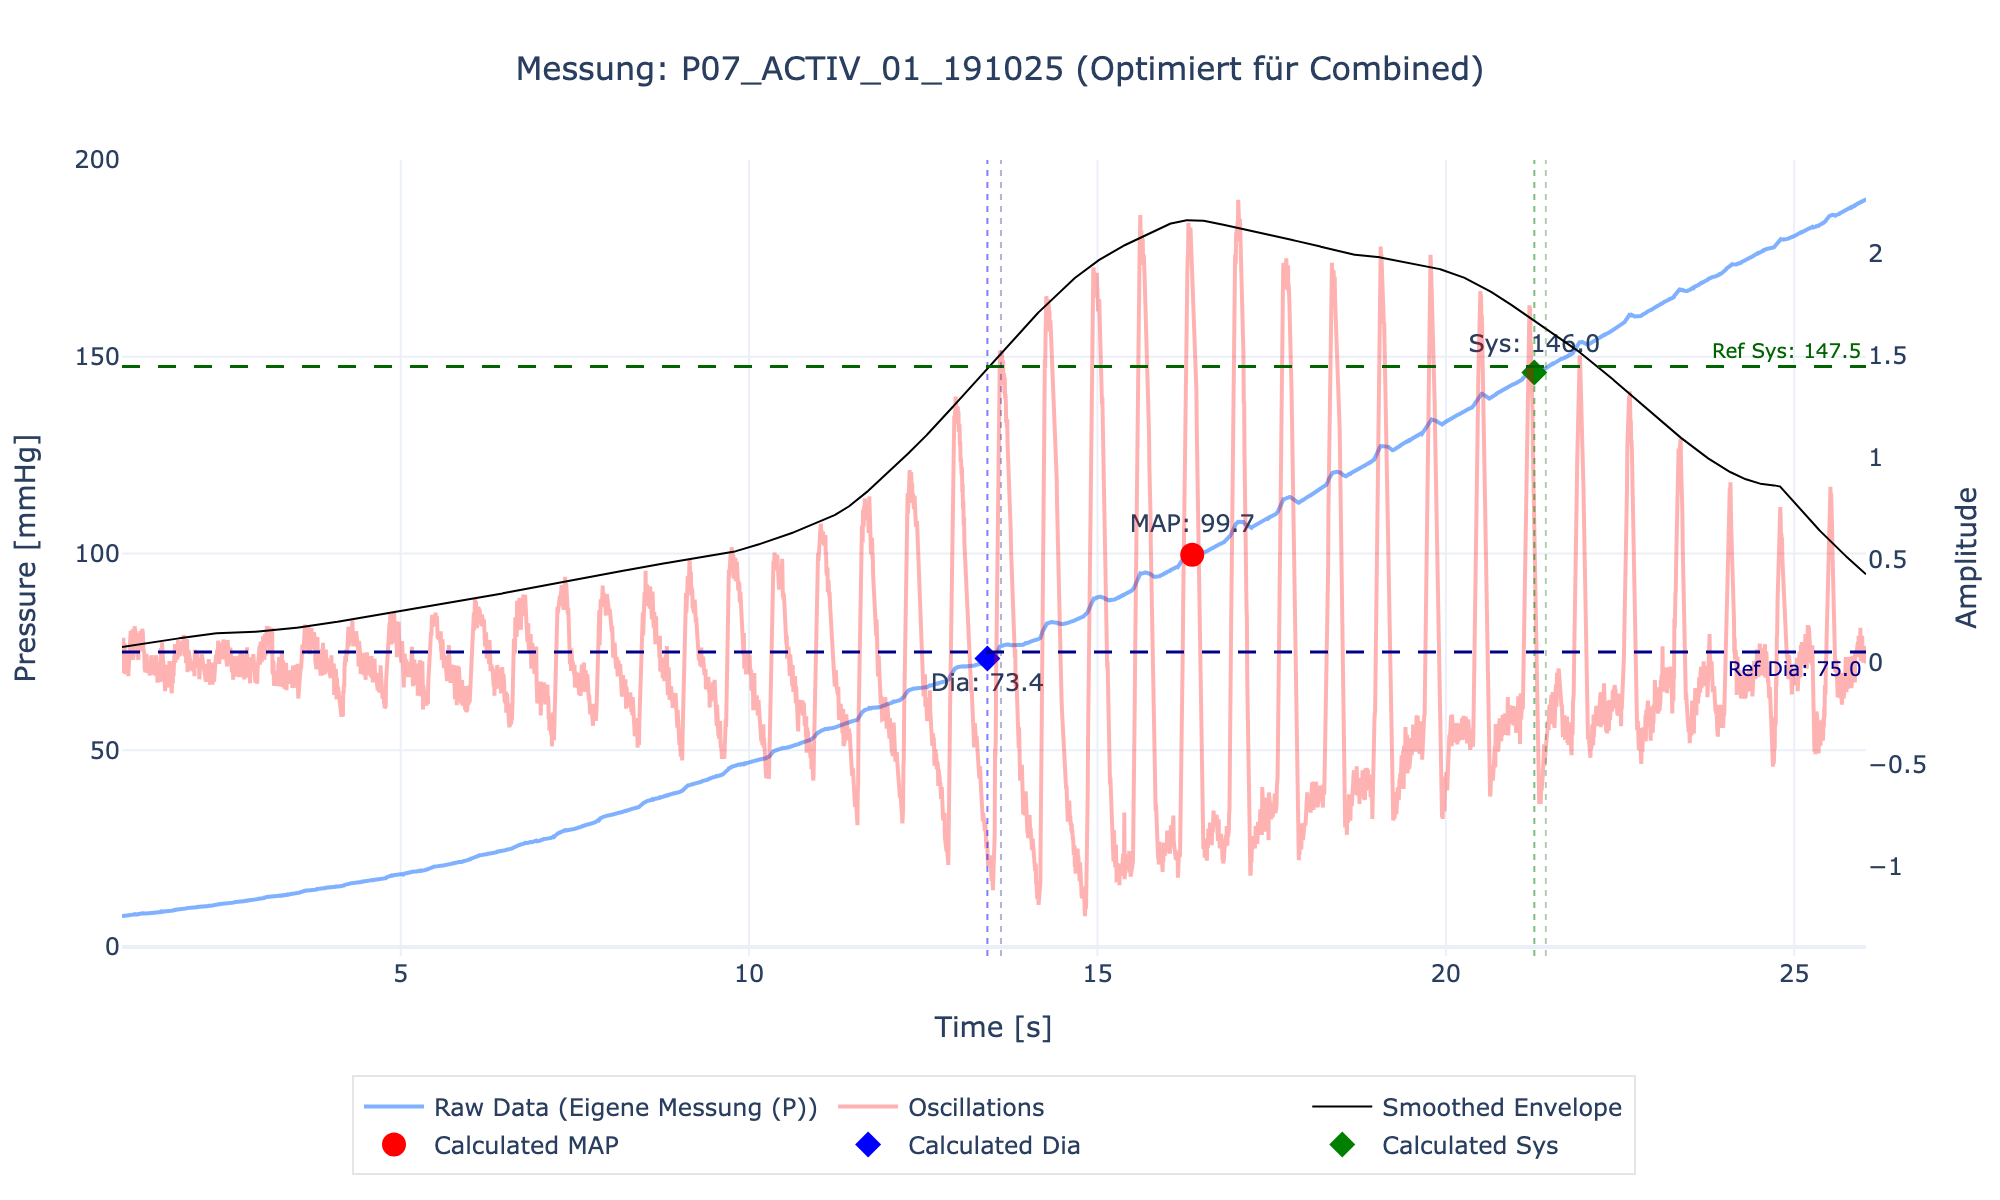
\includegraphics[width=\textwidth]{images/P07_ACTIV_01_191025_combined.png}
        \caption{Optimiert für Beurer und NAIS (Kombiniert)}
    \end{subfigure} \\
    \begin{subfigure}[b]{0.48\textwidth}
        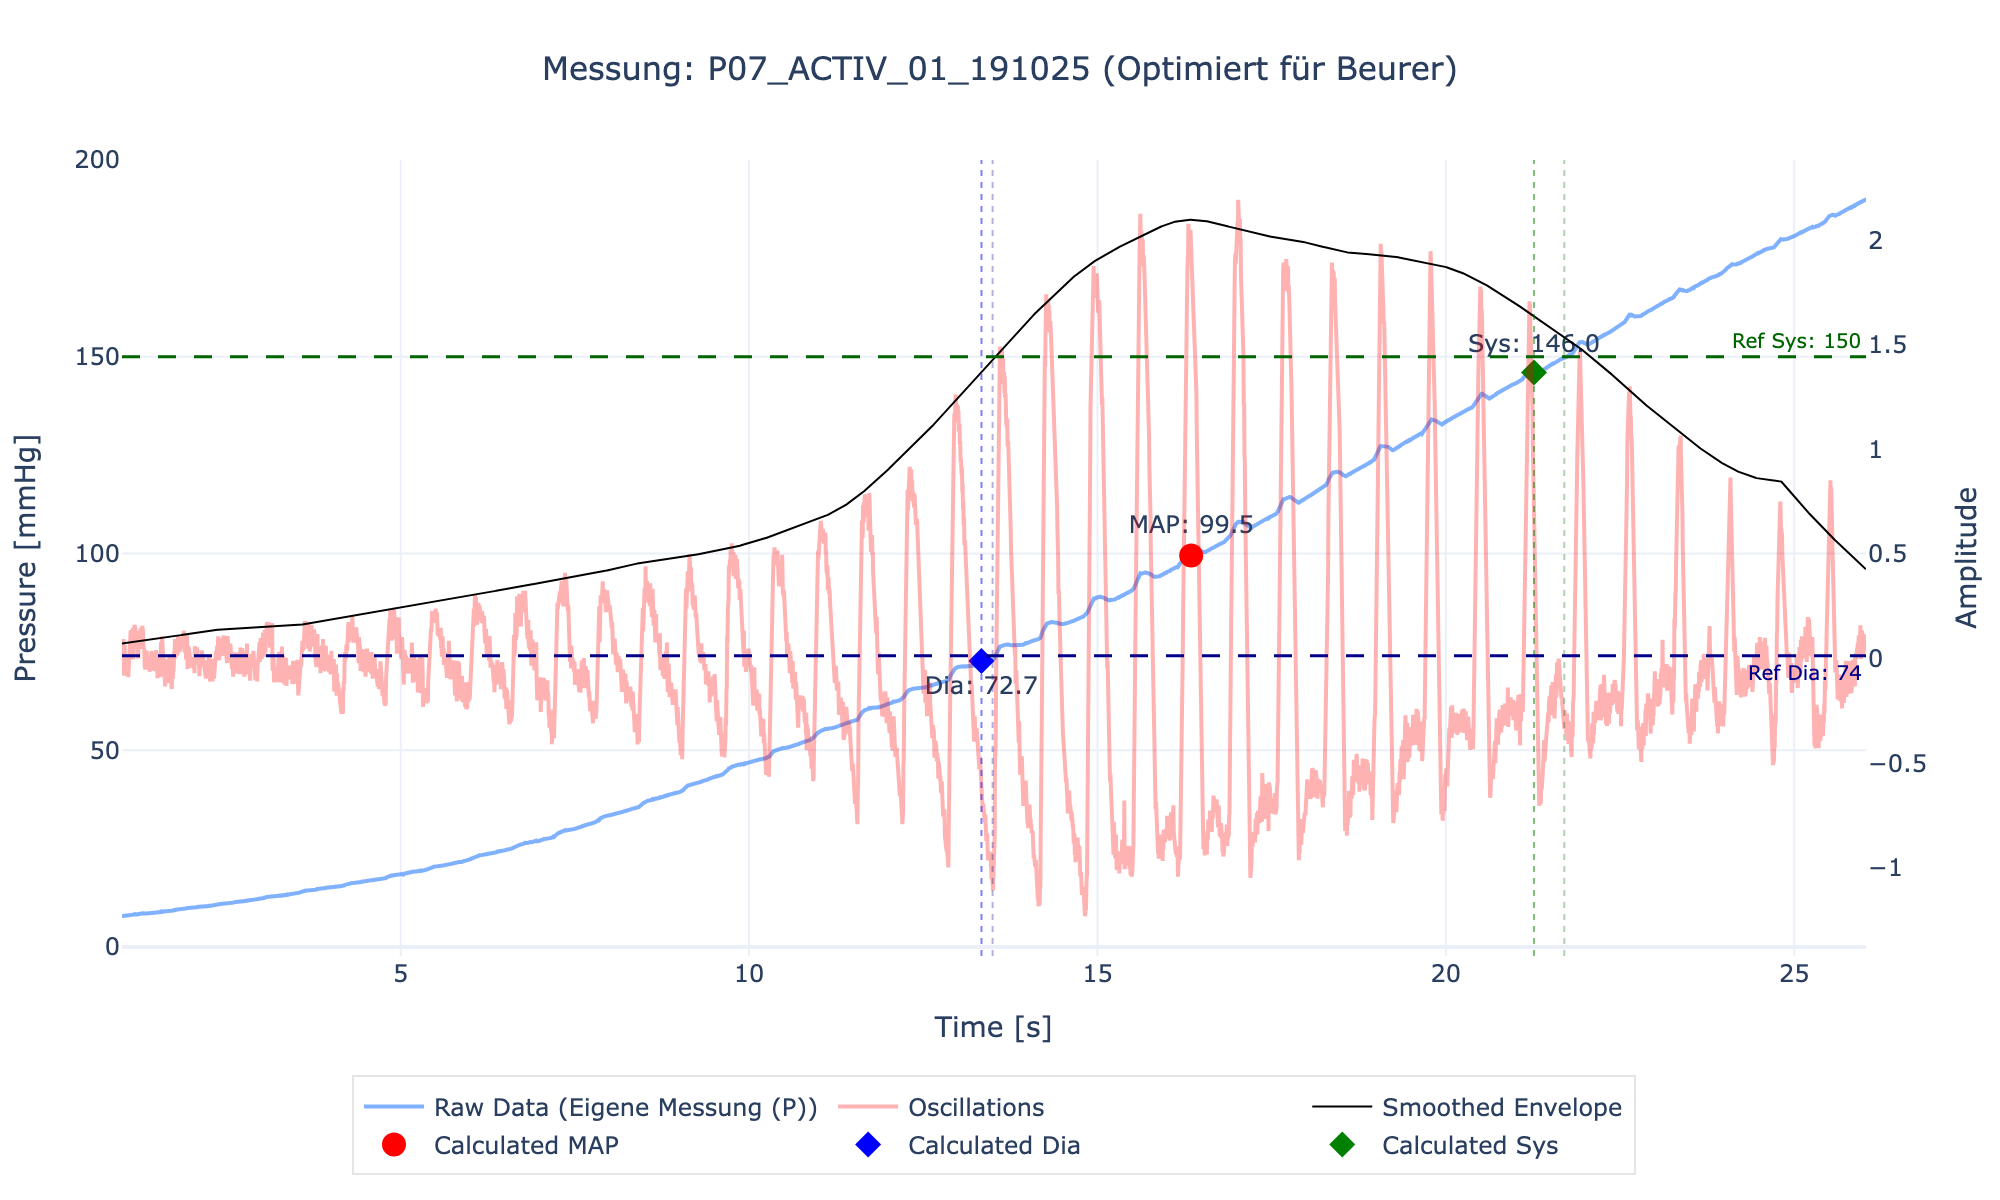
\includegraphics[width=\textwidth]{images/P07_ACTIV_01_191025_beurer.png}
        \caption{Optimiert für Beurer}
    \end{subfigure}
    \hfill
    \begin{subfigure}[b]{0.48\textwidth}
        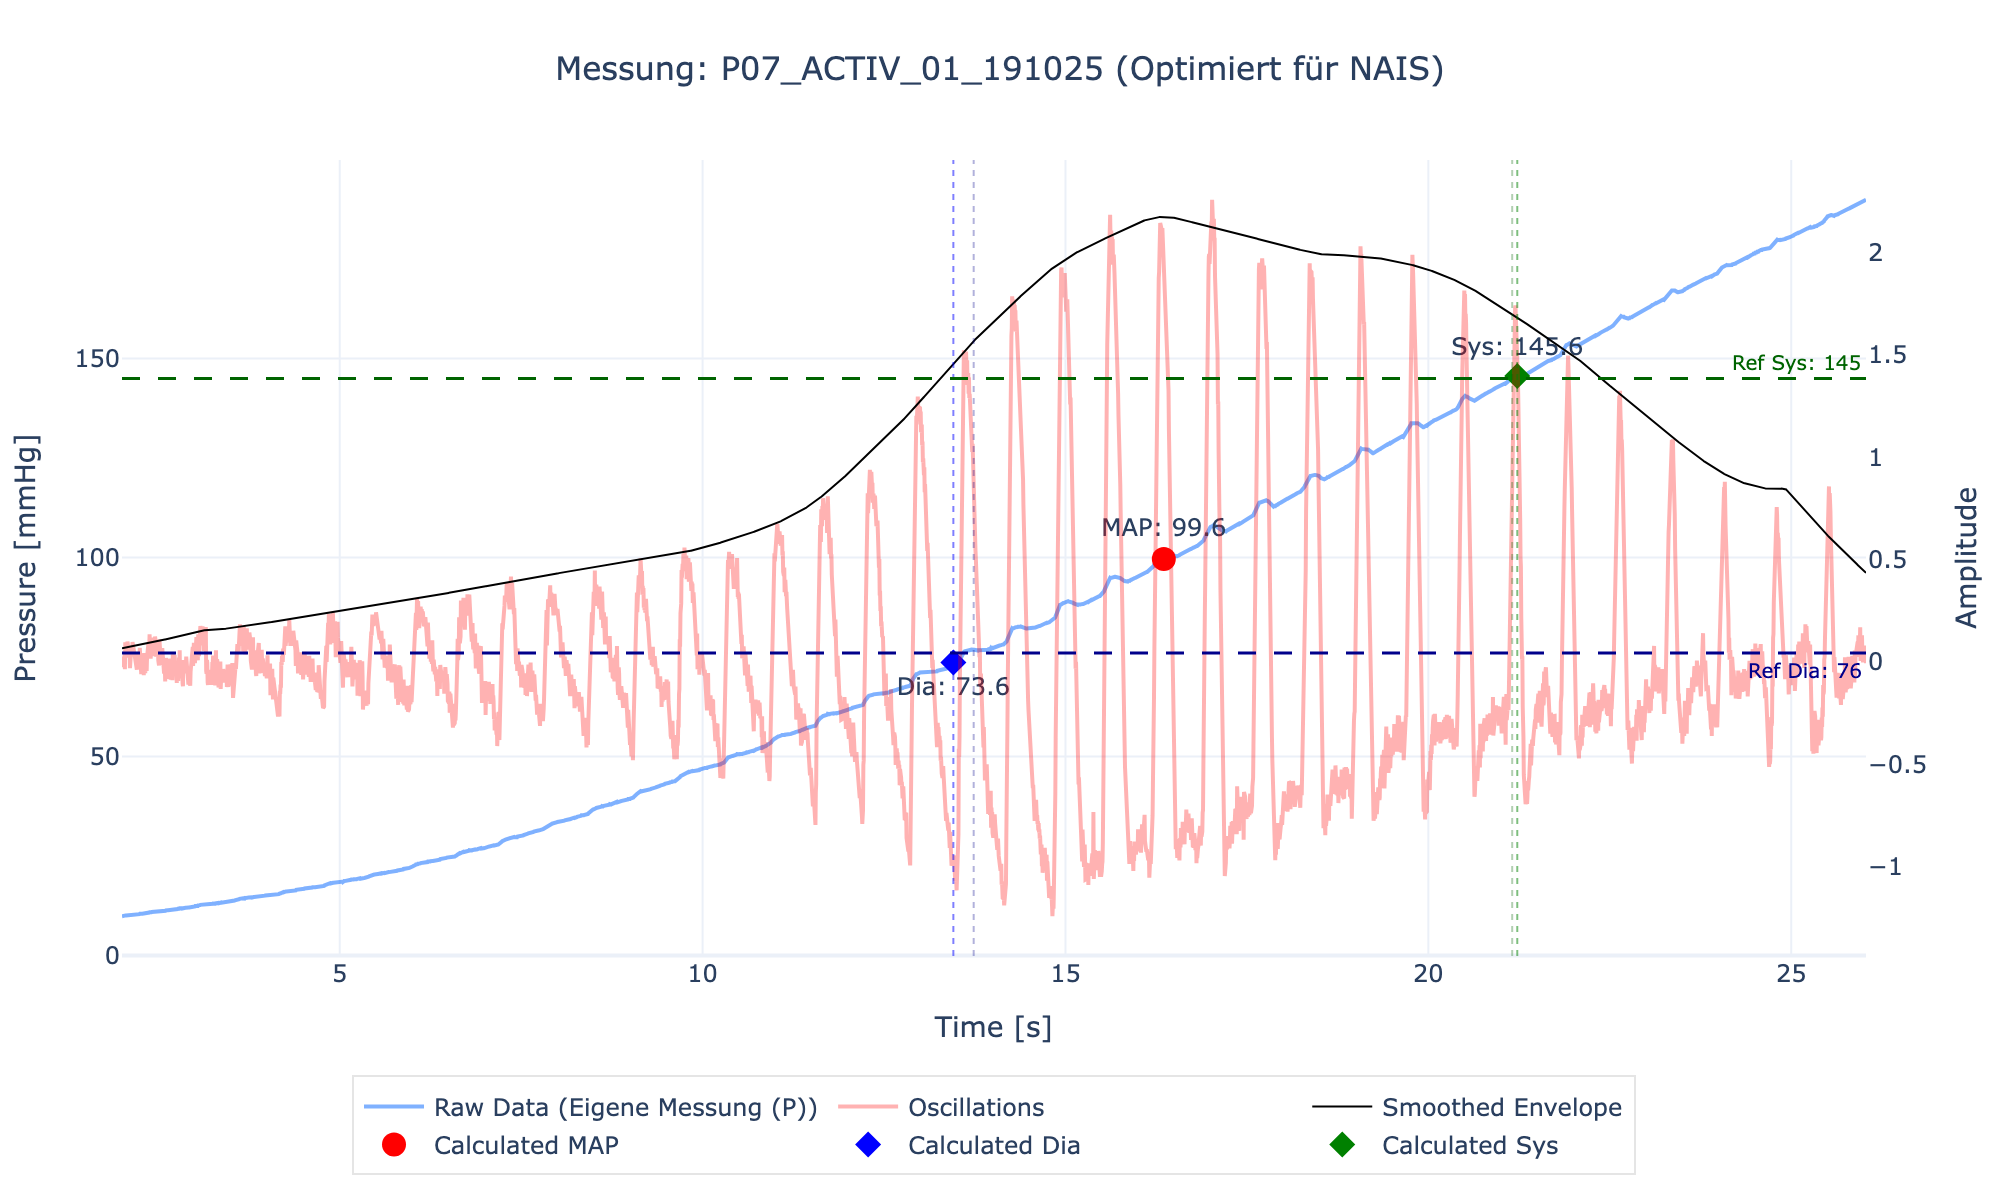
\includegraphics[width=\textwidth]{images/P07_ACTIV_01_191025_nais.png}
        \caption{Optimiert für NAIS}
    \end{subfigure}
    \caption{Einzelauswertung der Messung P07\_ACTIV\_01\_191025 mit verschiedenen Parametersätzen.}
\end{figure}
\newpage

\subsection*{Messung: P07\_REST\_01\_191025}
\begin{figure}[H]
    \centering
    \begin{subfigure}[b]{0.8\textwidth}
        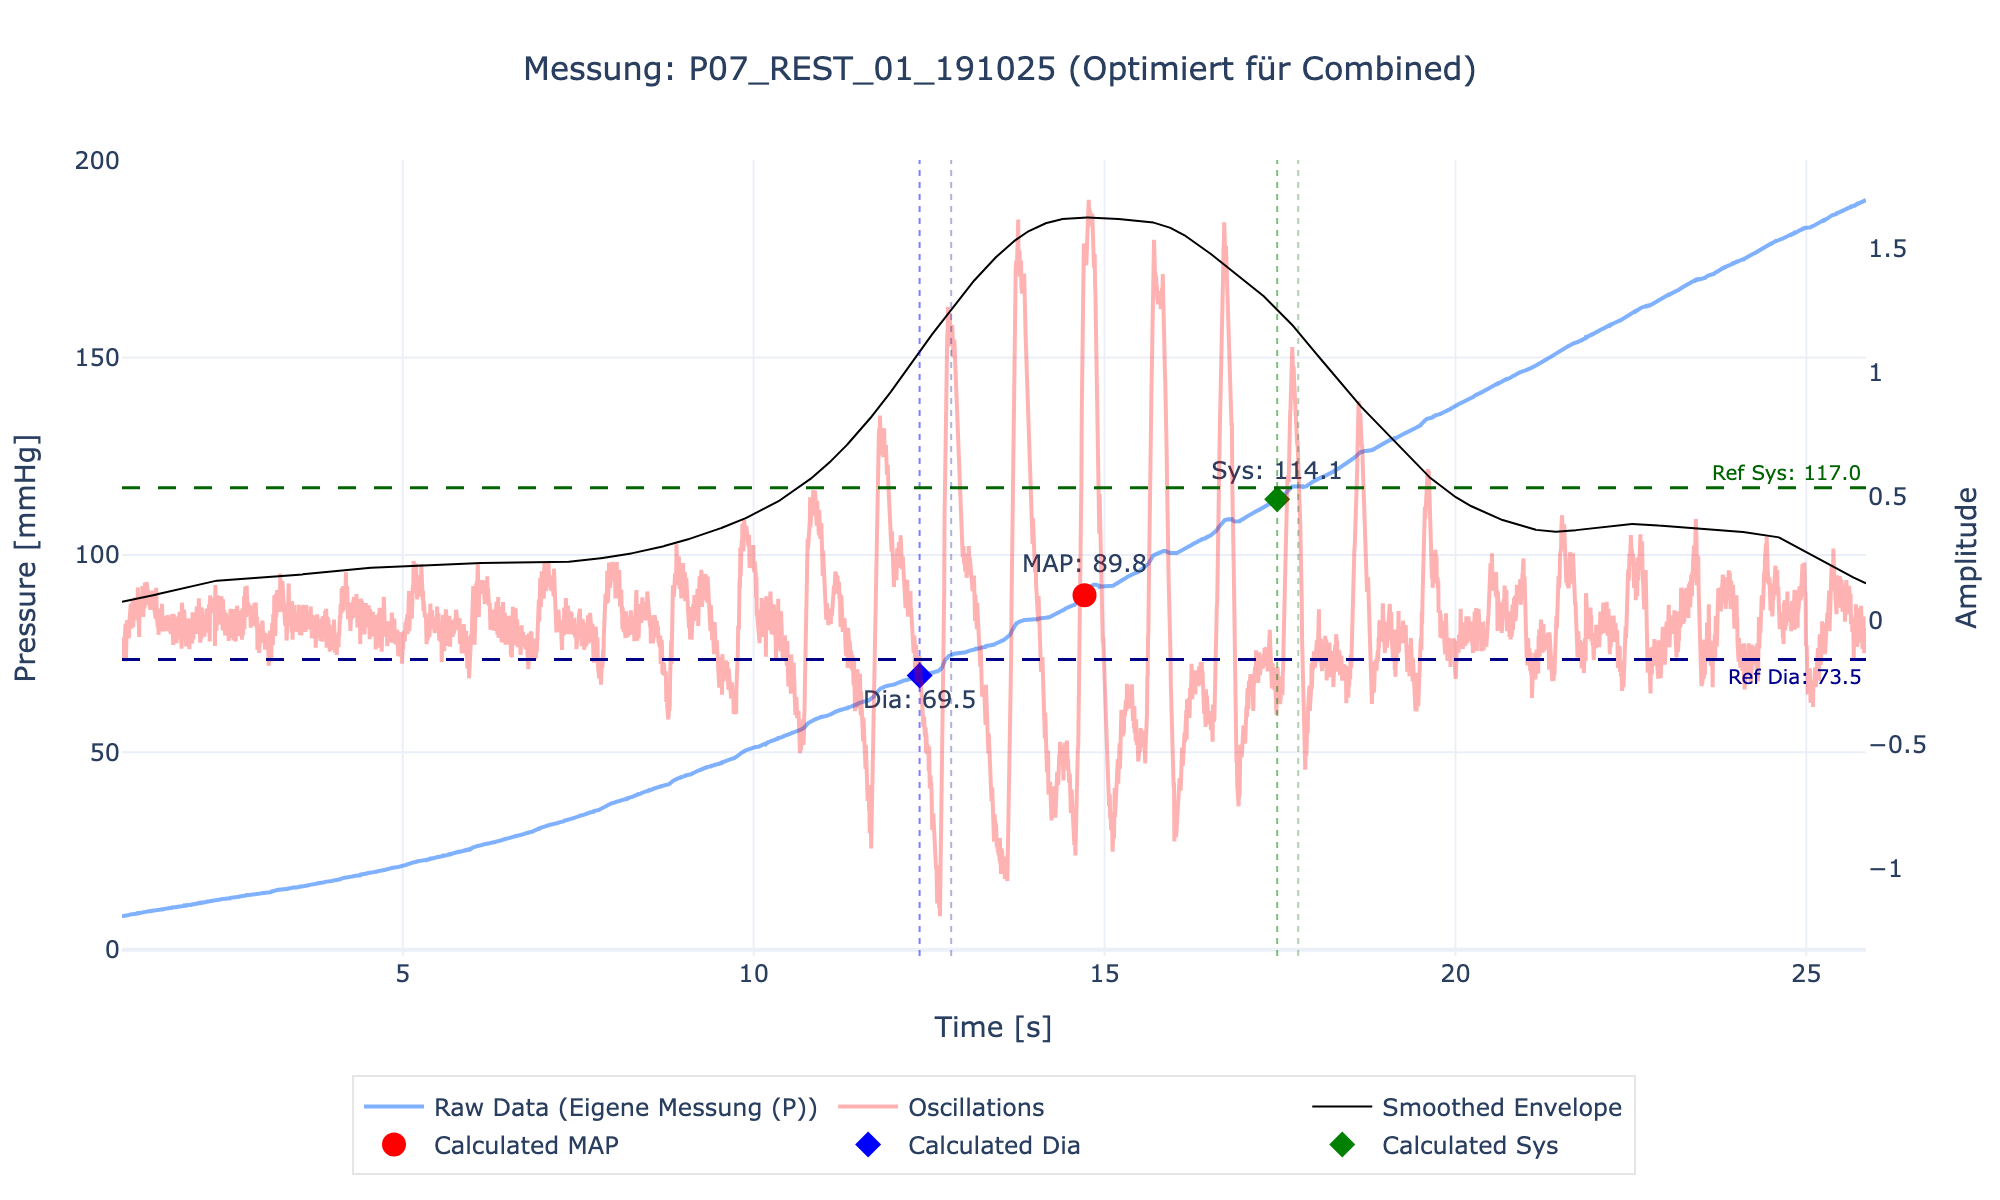
\includegraphics[width=\textwidth]{images/P07_REST_01_191025_combined.png}
        \caption{Optimiert für Beurer und NAIS (Kombiniert)}
    \end{subfigure} \\
    \begin{subfigure}[b]{0.48\textwidth}
        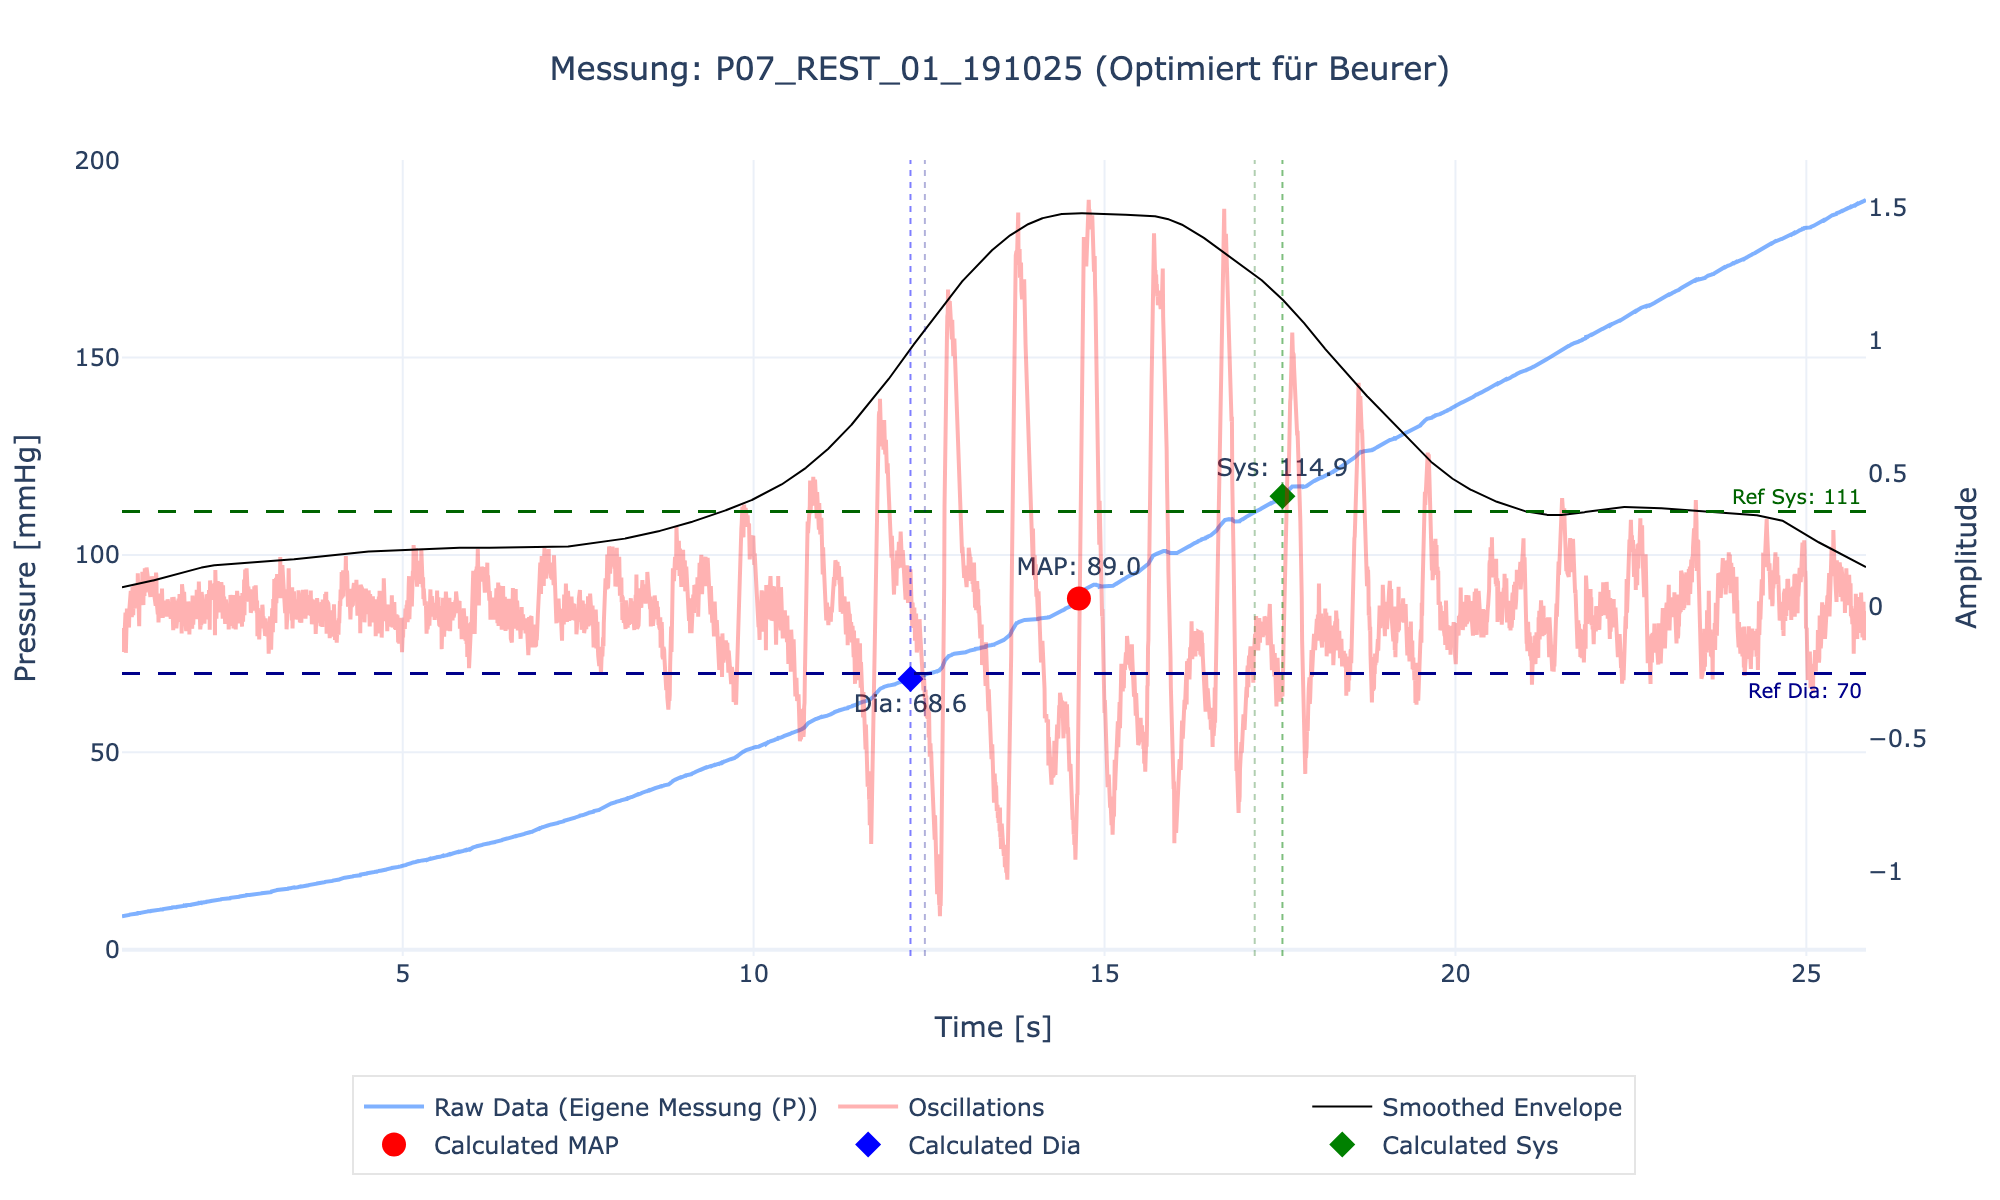
\includegraphics[width=\textwidth]{images/P07_REST_01_191025_beurer.png}
        \caption{Optimiert für Beurer}
    \end{subfigure}
    \hfill
    \begin{subfigure}[b]{0.48\textwidth}
        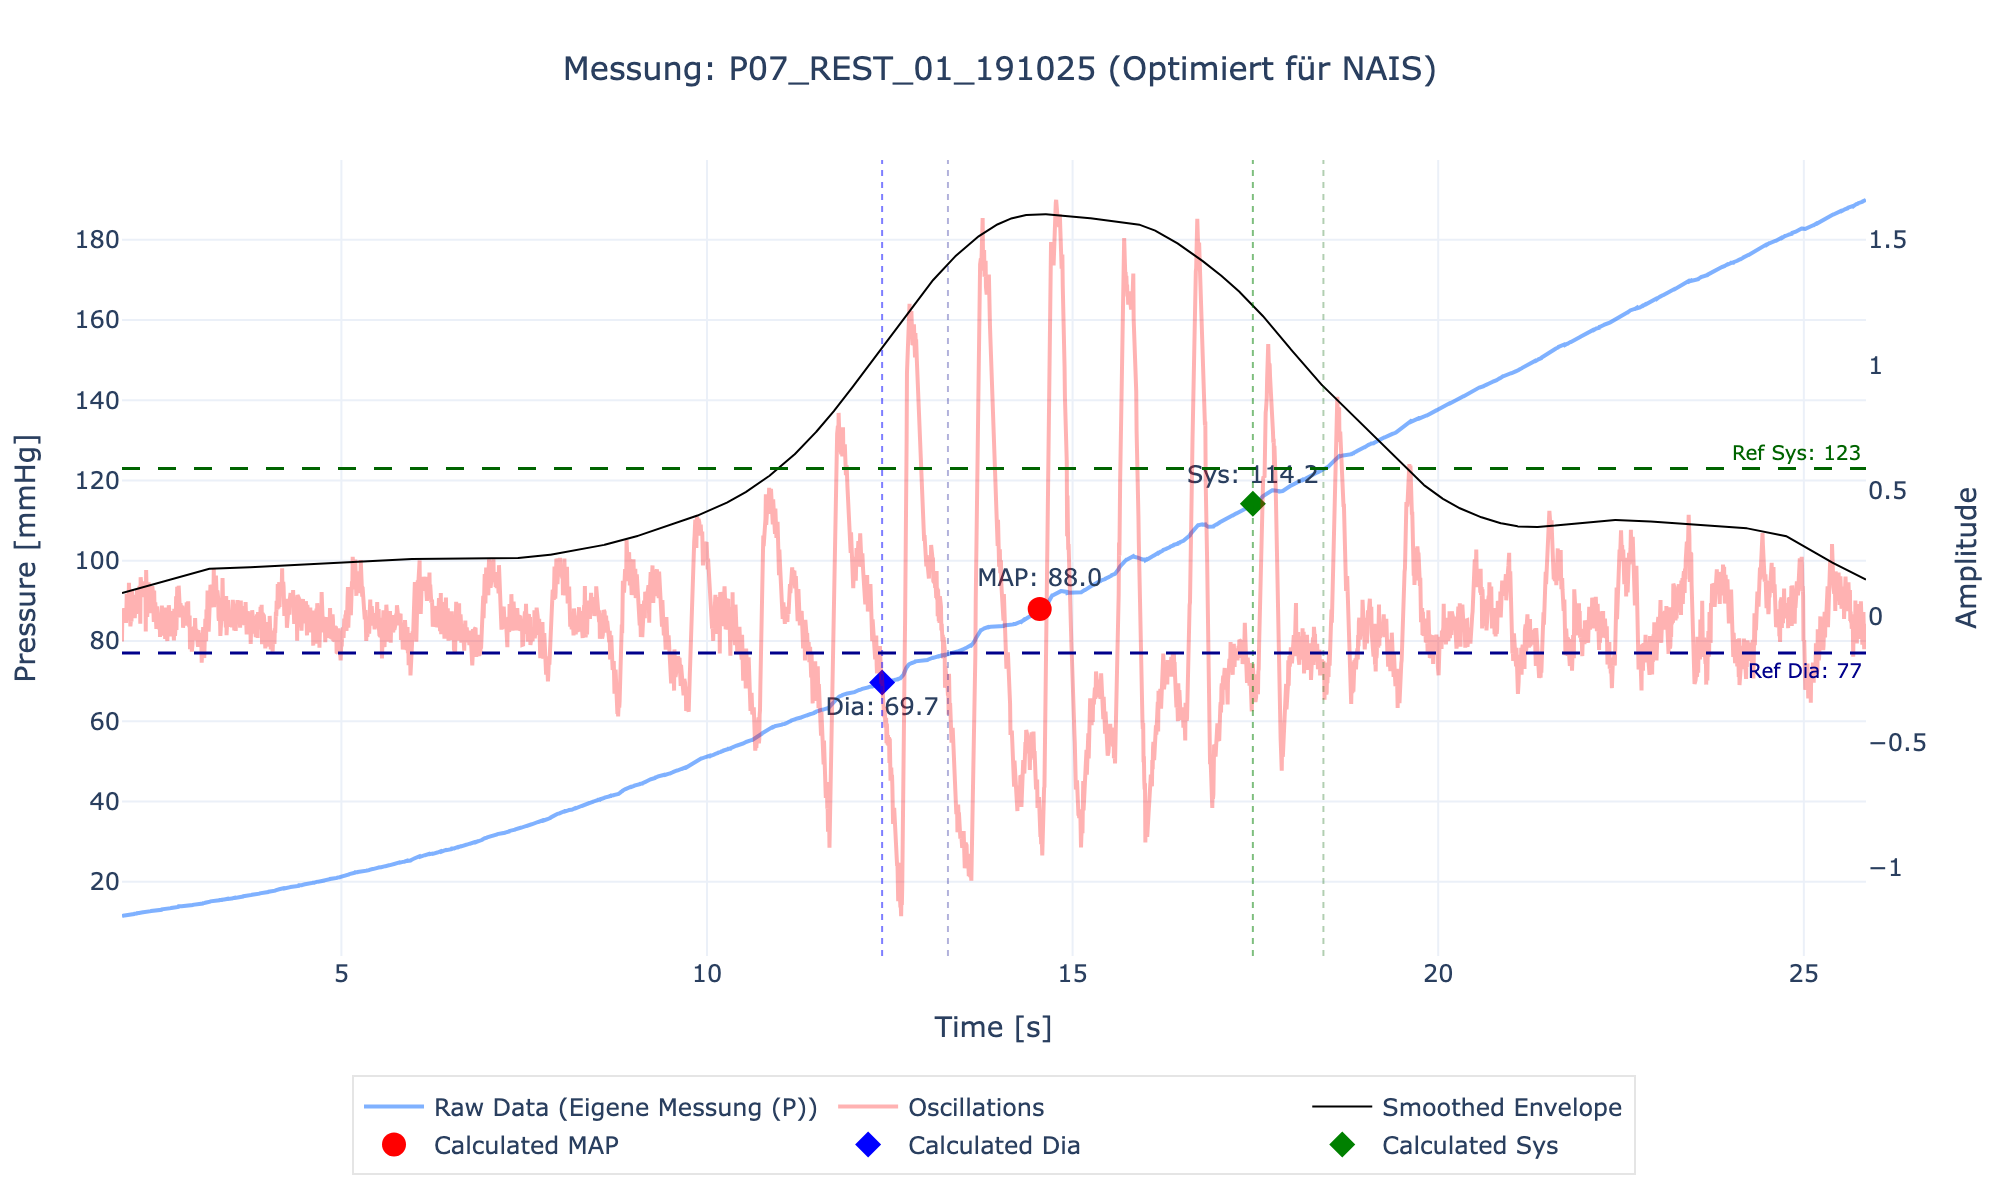
\includegraphics[width=\textwidth]{images/P07_REST_01_191025_nais.png}
        \caption{Optimiert für NAIS}
    \end{subfigure}
    \caption{Einzelauswertung der Messung P07\_REST\_01\_191025 mit verschiedenen Parametersätzen.}
\end{figure}
\newpage

\subsection*{Messung: P08\_ACTIV\_01\_201025}
\begin{figure}[H]
    \centering
    \begin{subfigure}[b]{0.8\textwidth}
        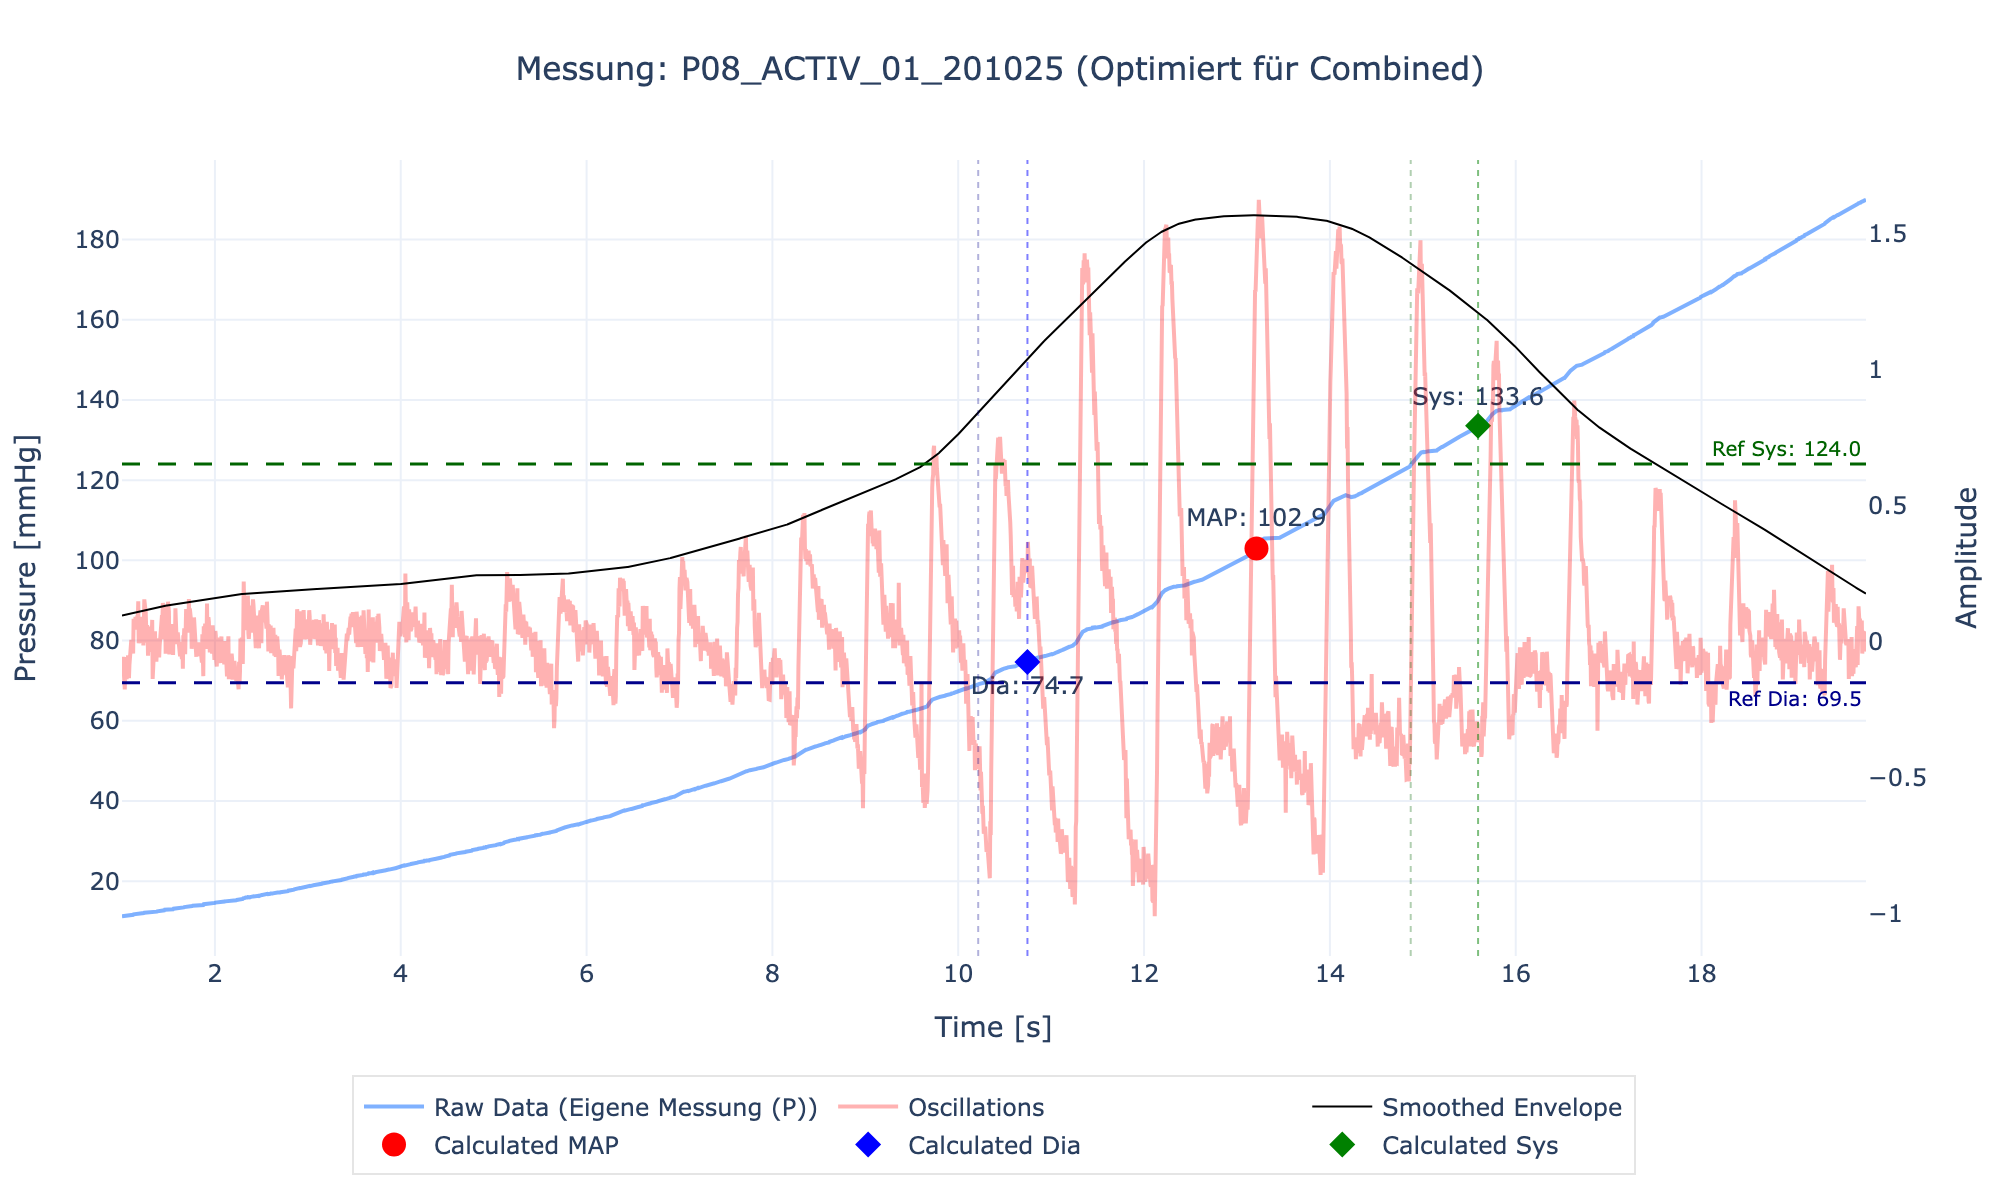
\includegraphics[width=\textwidth]{images/P08_ACTIV_01_201025_combined.png}
        \caption{Optimiert für Beurer und NAIS (Kombiniert)}
    \end{subfigure} \\
    \begin{subfigure}[b]{0.48\textwidth}
        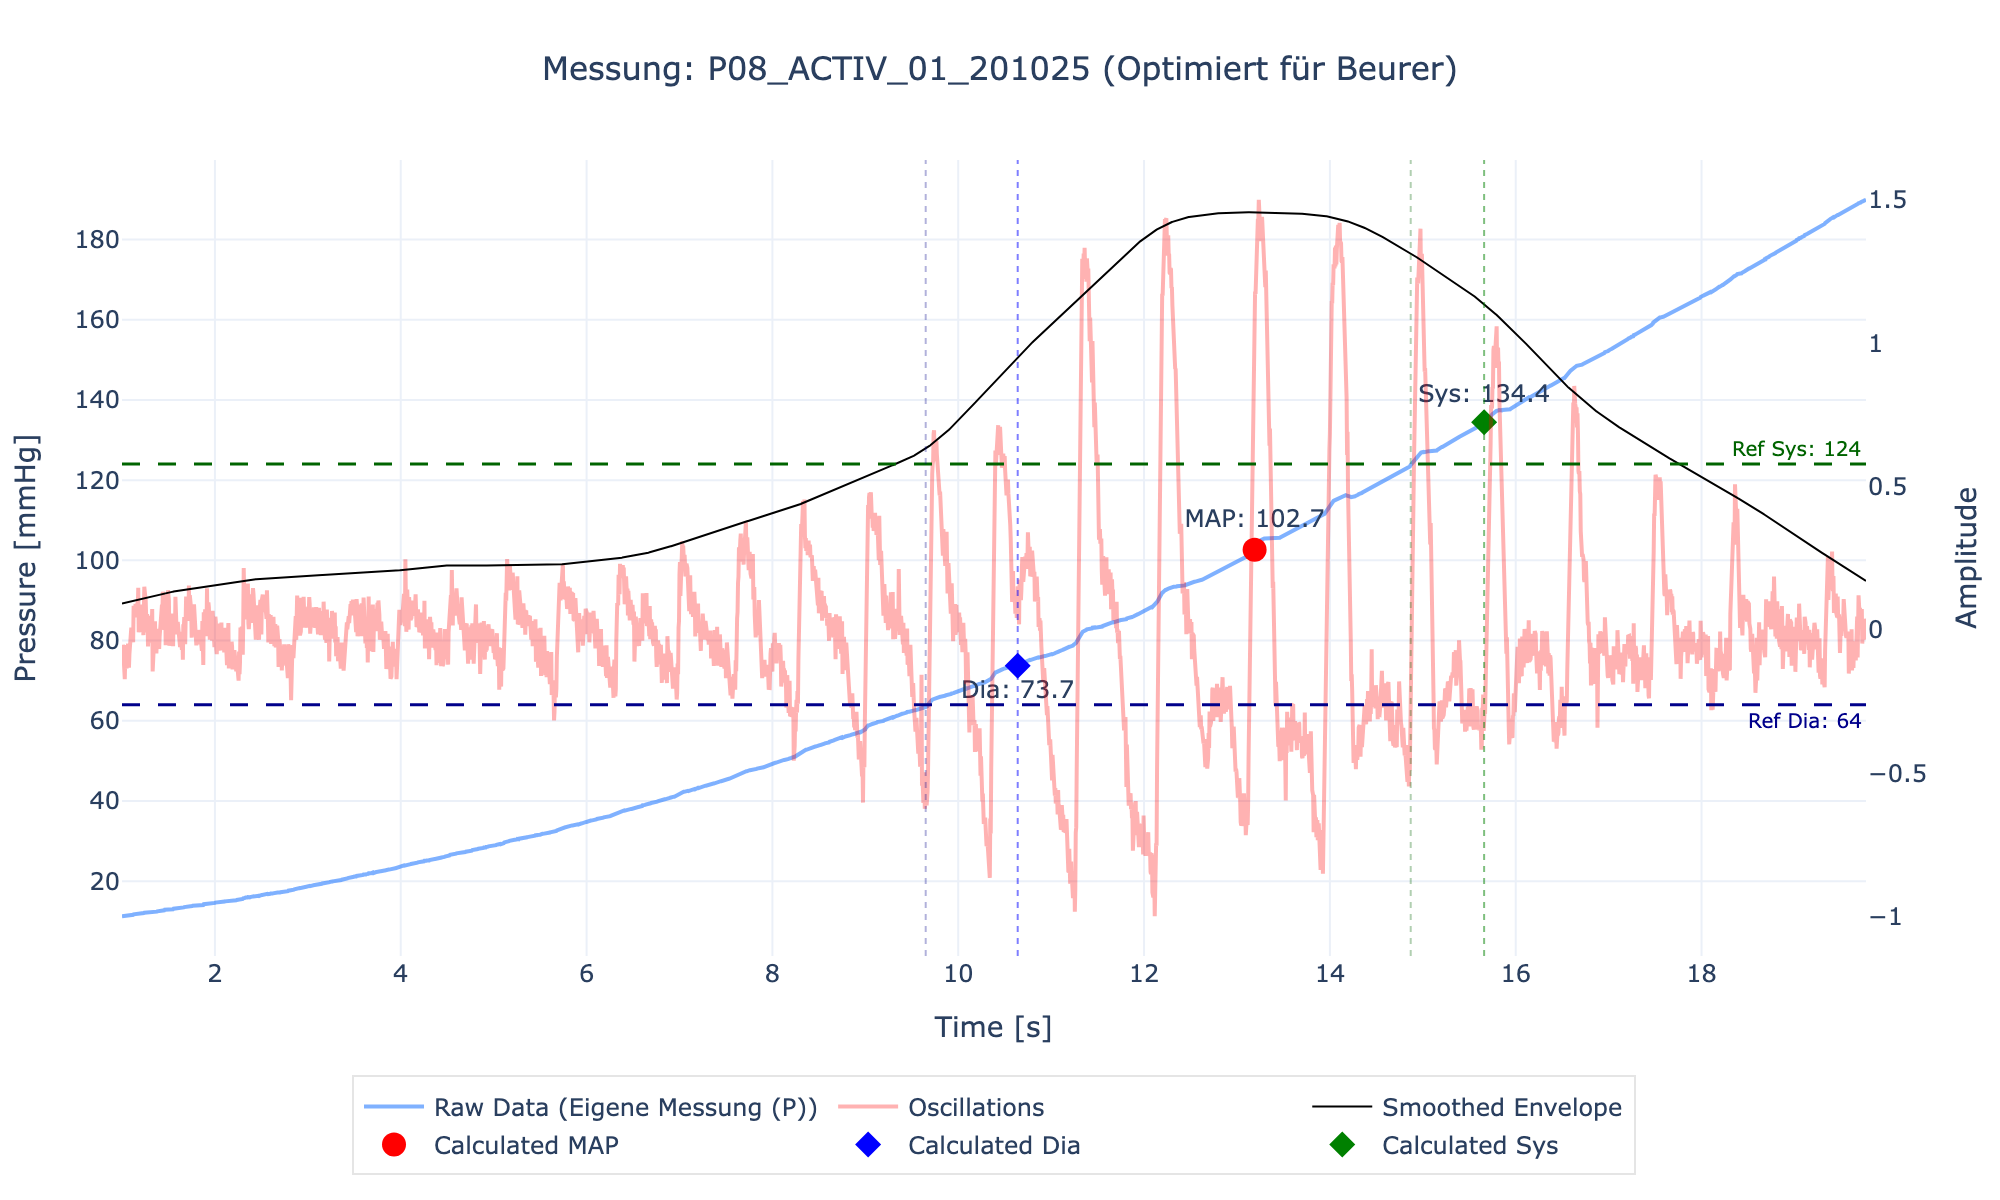
\includegraphics[width=\textwidth]{images/P08_ACTIV_01_201025_beurer.png}
        \caption{Optimiert für Beurer}
    \end{subfigure}
    \hfill
    \begin{subfigure}[b]{0.48\textwidth}
        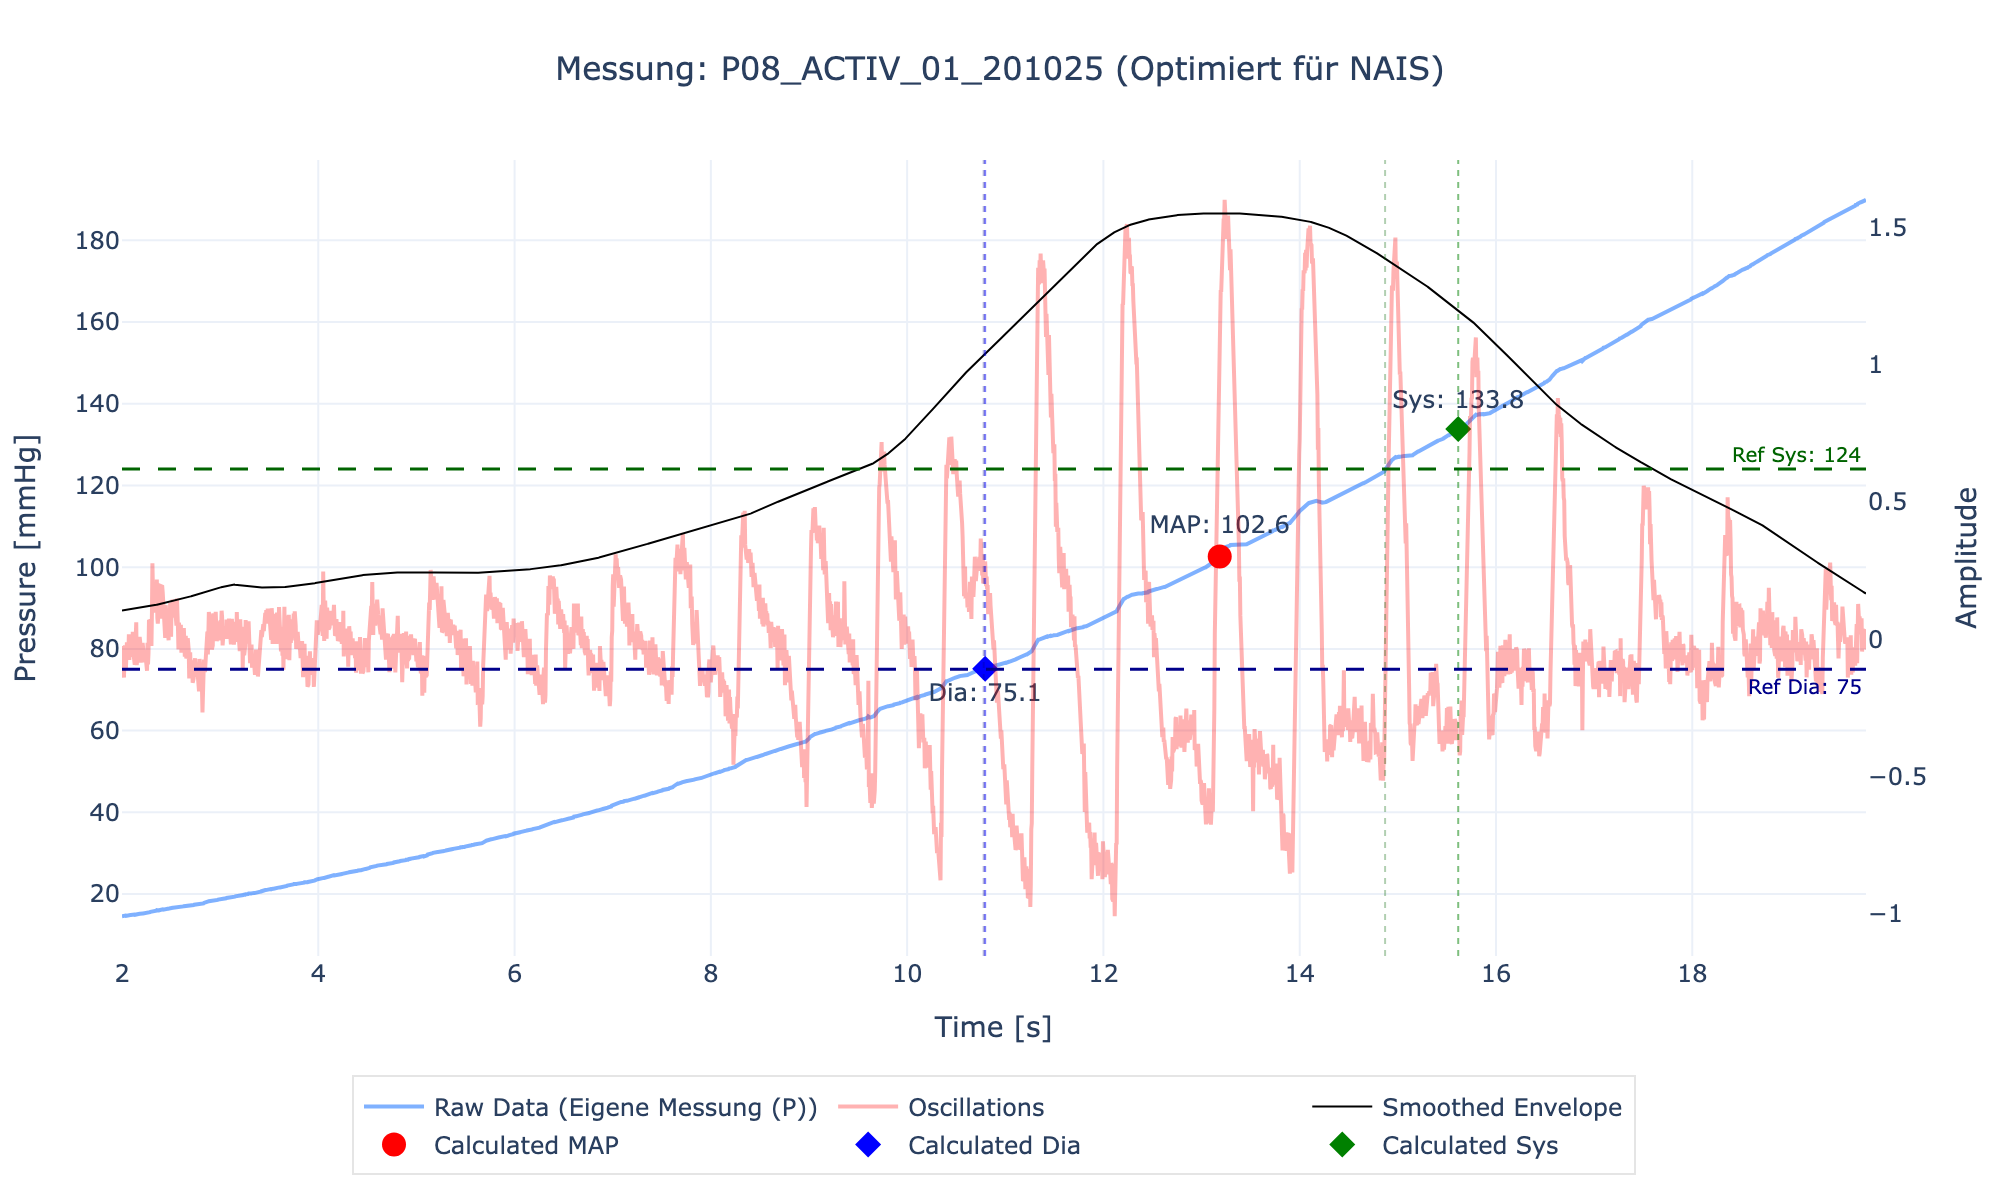
\includegraphics[width=\textwidth]{images/P08_ACTIV_01_201025_nais.png}
        \caption{Optimiert für NAIS}
    \end{subfigure}
    \caption{Einzelauswertung der Messung P08\_ACTIV\_01\_201025 mit verschiedenen Parametersätzen.}
\end{figure}
\newpage

\subsection*{Messung: P08\_REST\_01\_201025}
\begin{figure}[H]
    \centering
    \begin{subfigure}[b]{0.8\textwidth}
        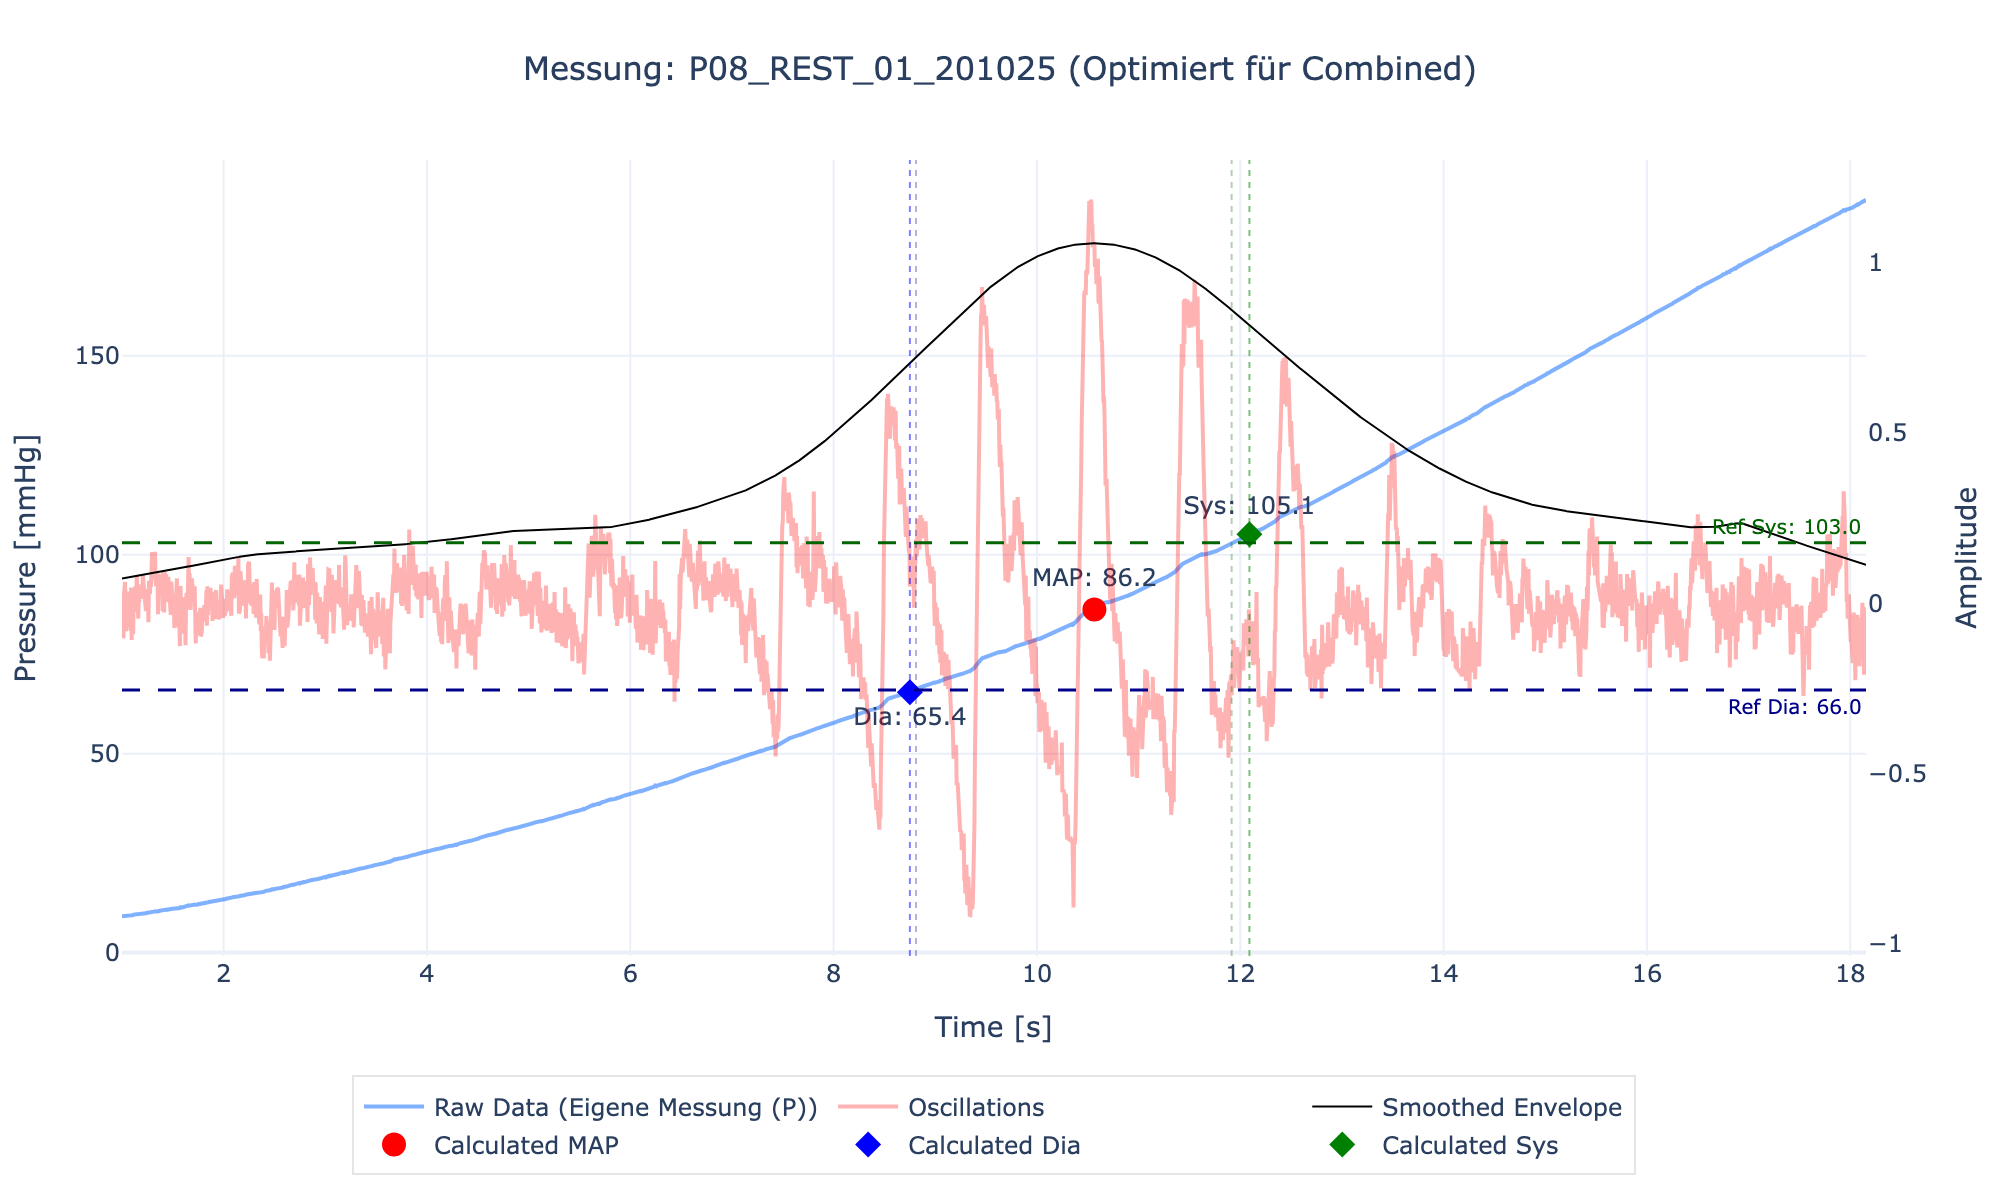
\includegraphics[width=\textwidth]{images/P08_REST_01_201025_combined.png}
        \caption{Optimiert für Beurer und NAIS (Kombiniert)}
    \end{subfigure} \\
    \begin{subfigure}[b]{0.48\textwidth}
        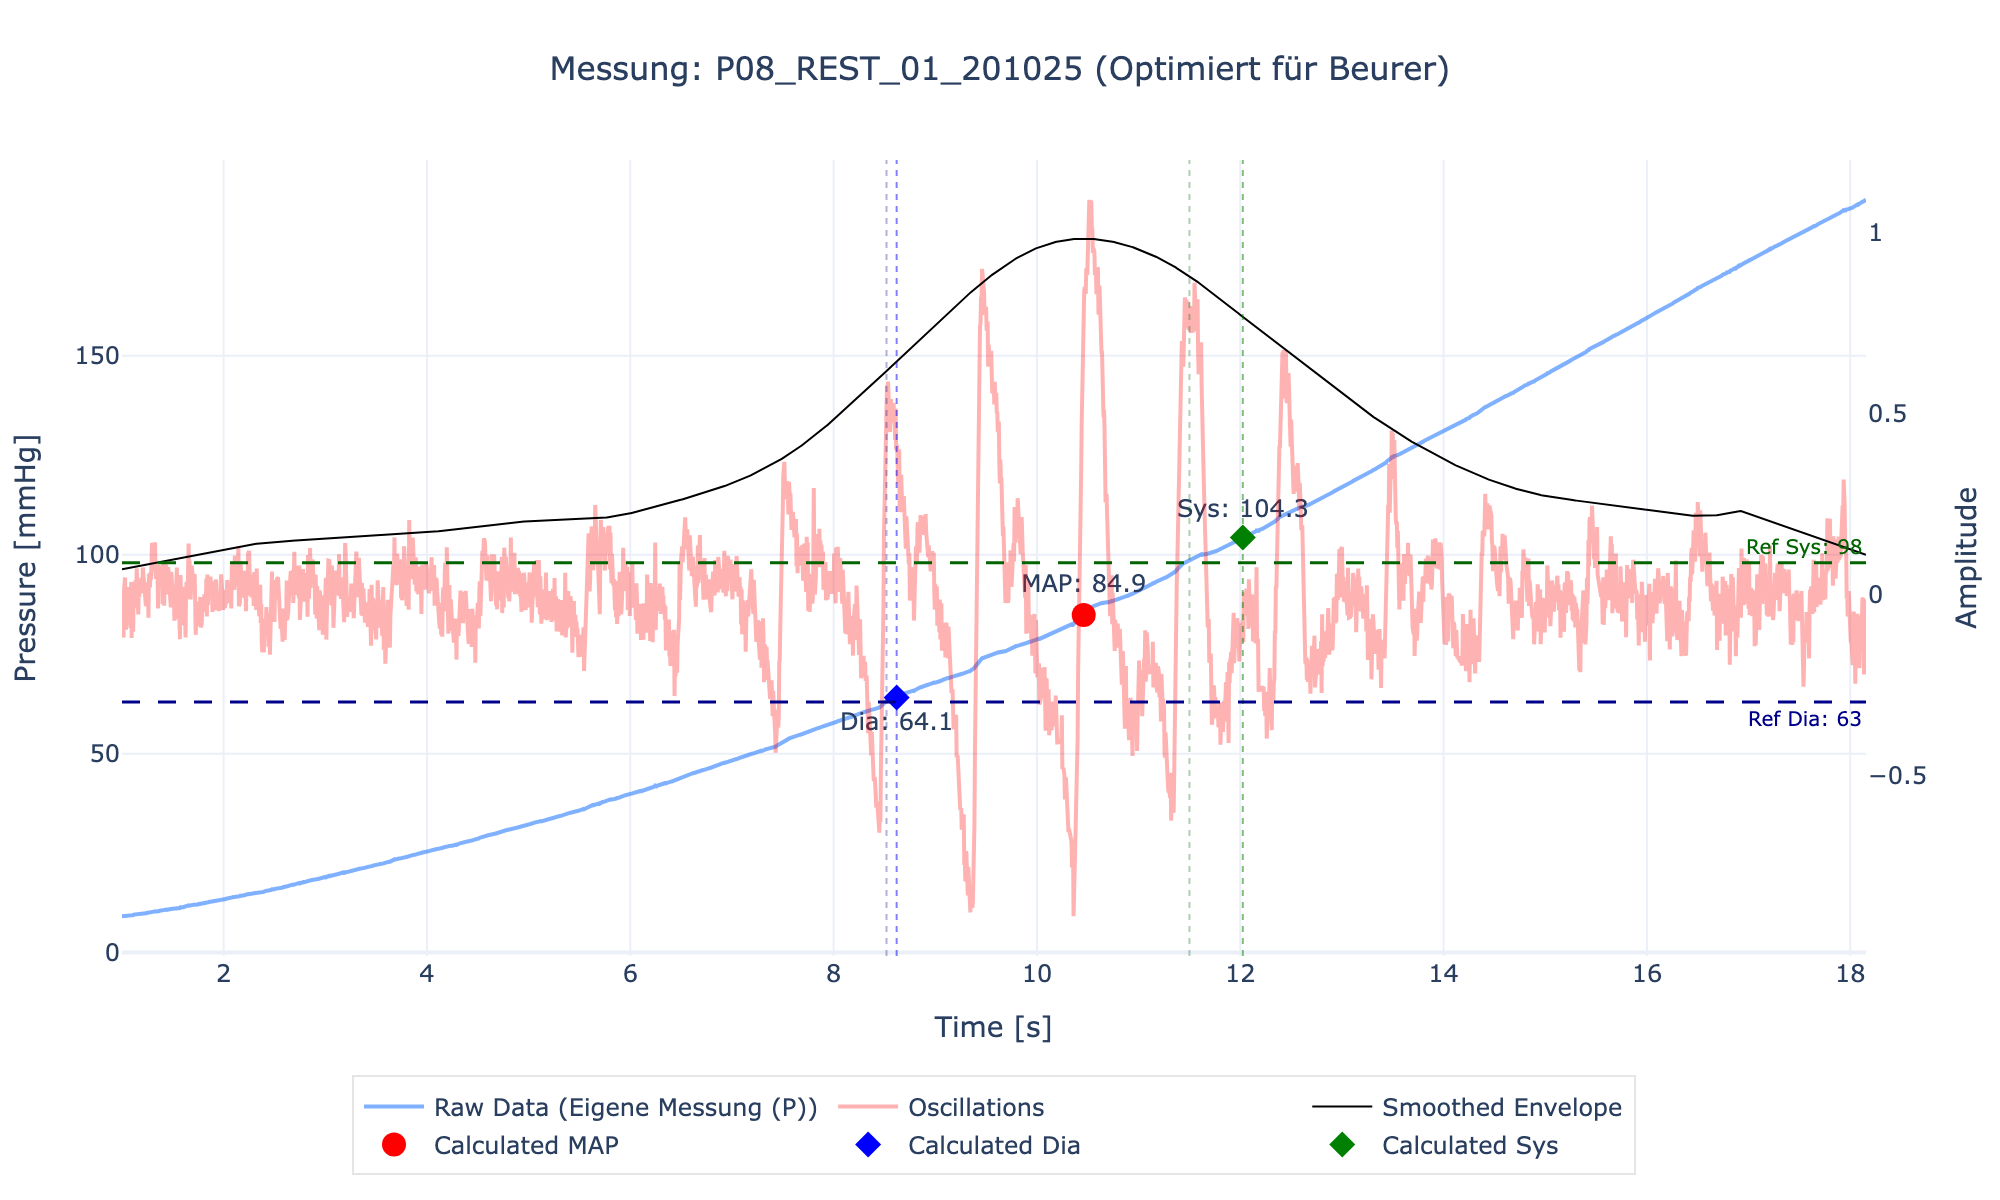
\includegraphics[width=\textwidth]{images/P08_REST_01_201025_beurer.png}
        \caption{Optimiert für Beurer}
    \end{subfigure}
    \hfill
    \begin{subfigure}[b]{0.48\textwidth}
        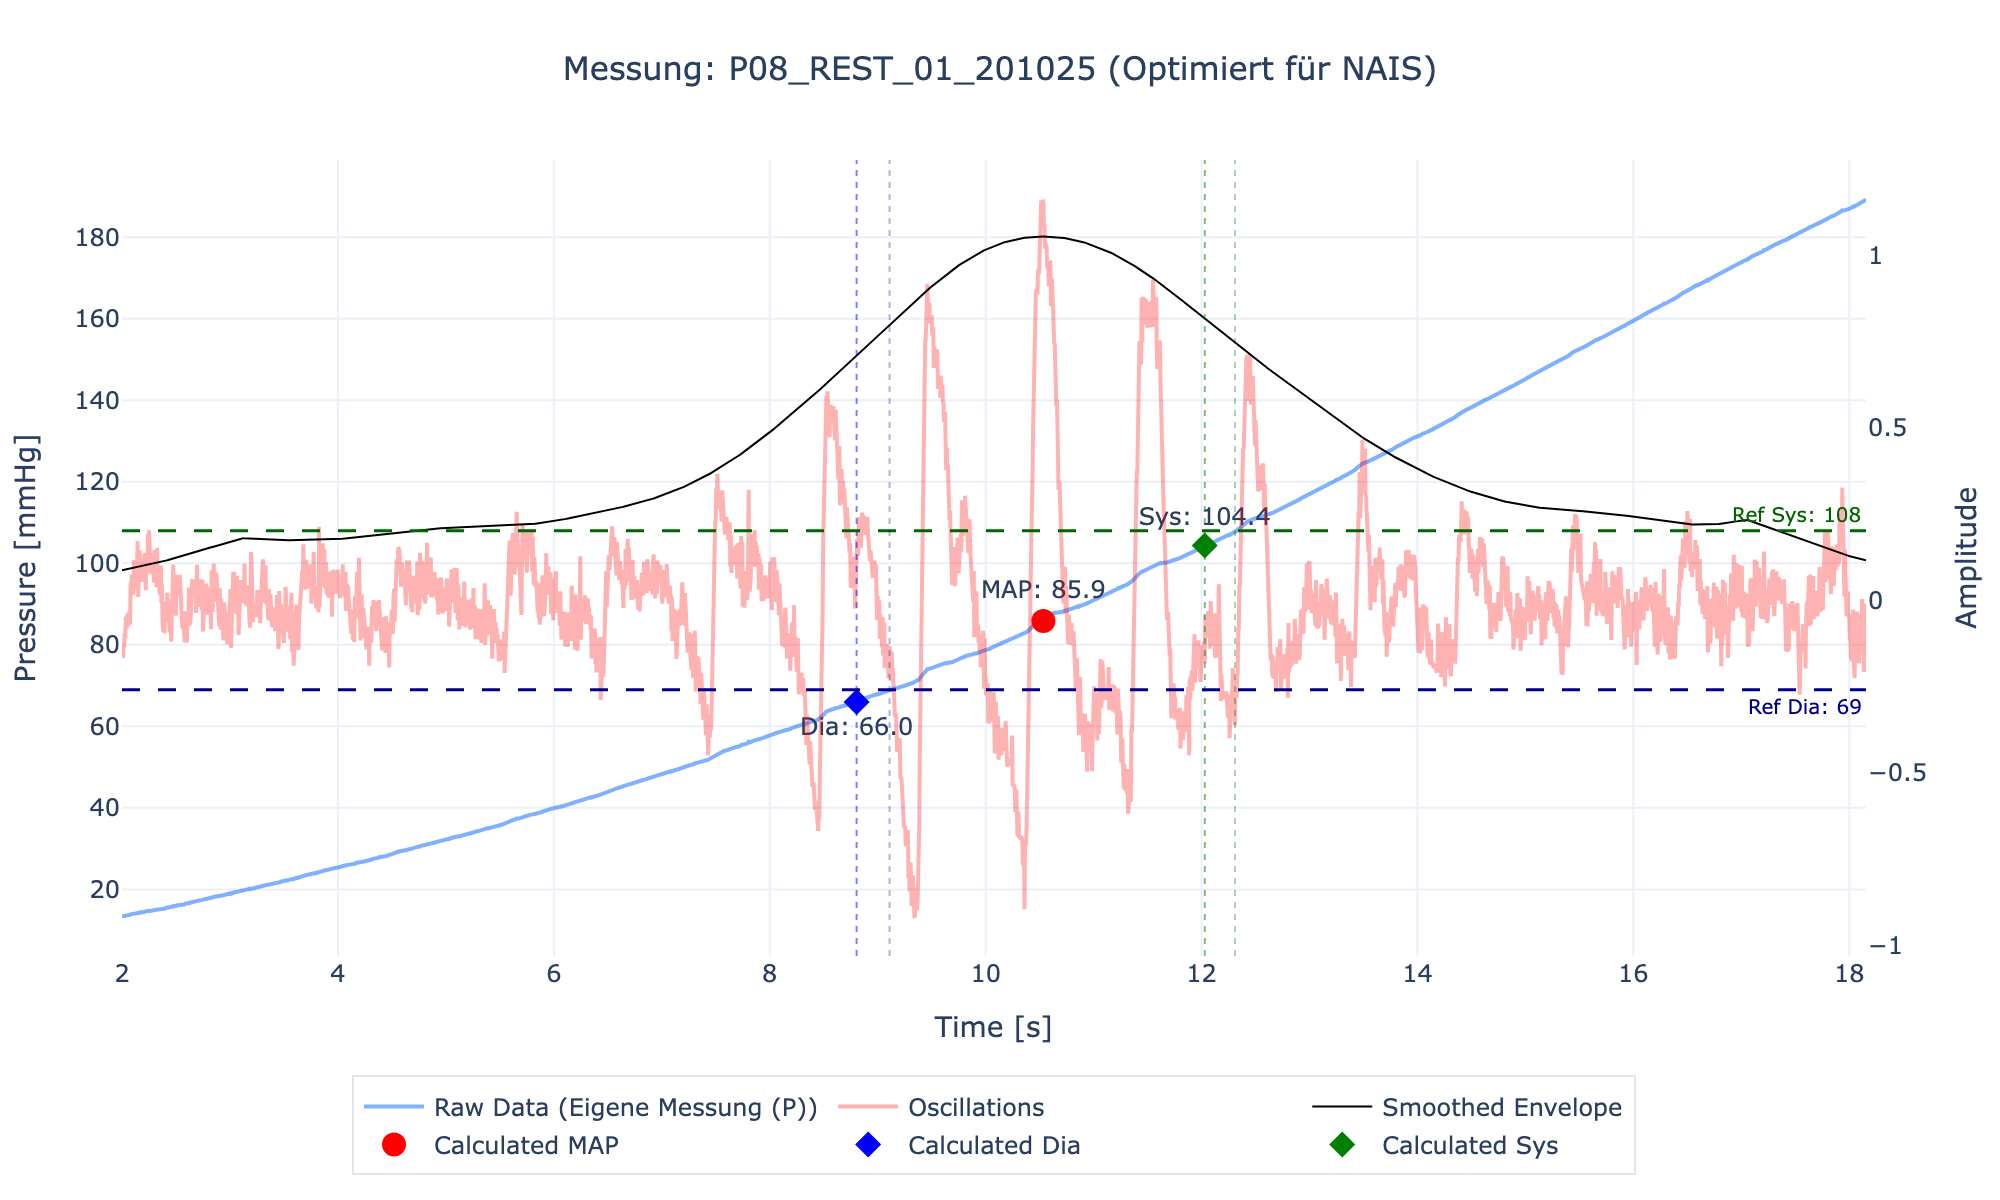
\includegraphics[width=\textwidth]{images/P08_REST_01_201025_nais.png}
        \caption{Optimiert für NAIS}
    \end{subfigure}
    \caption{Einzelauswertung der Messung P08\_REST\_01\_201025 mit verschiedenen Parametersätzen.}
\end{figure}
\newpage

\subsection*{Messung: S001-M001-Rest}
\begin{figure}[H]
    \centering
    \begin{subfigure}[b]{0.8\textwidth}
        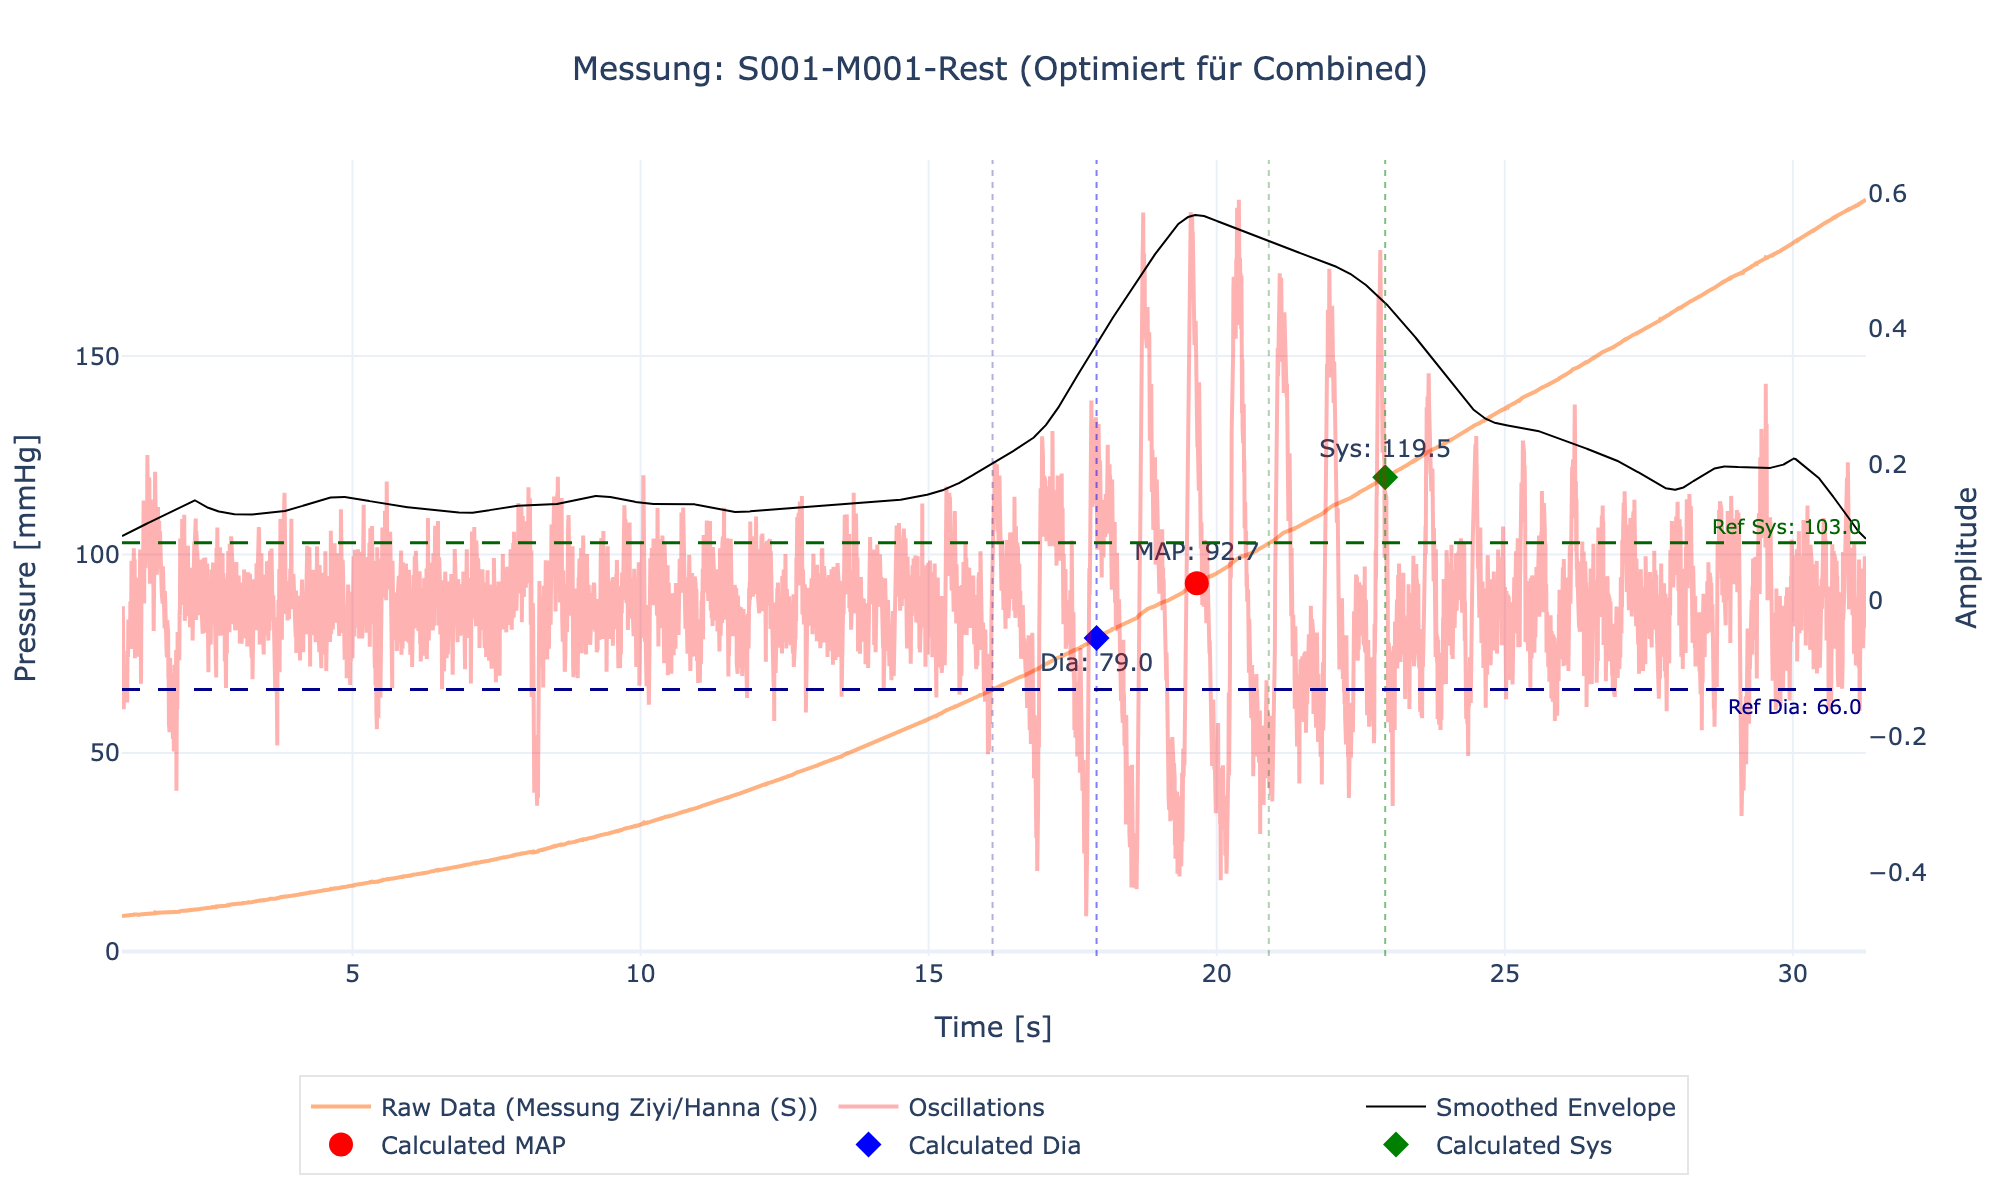
\includegraphics[width=\textwidth]{images/S001-M001-Rest_combined.png}
        \caption{Optimiert für Beurer und NAIS (Kombiniert)}
    \end{subfigure} \\
    \begin{subfigure}[b]{0.48\textwidth}
        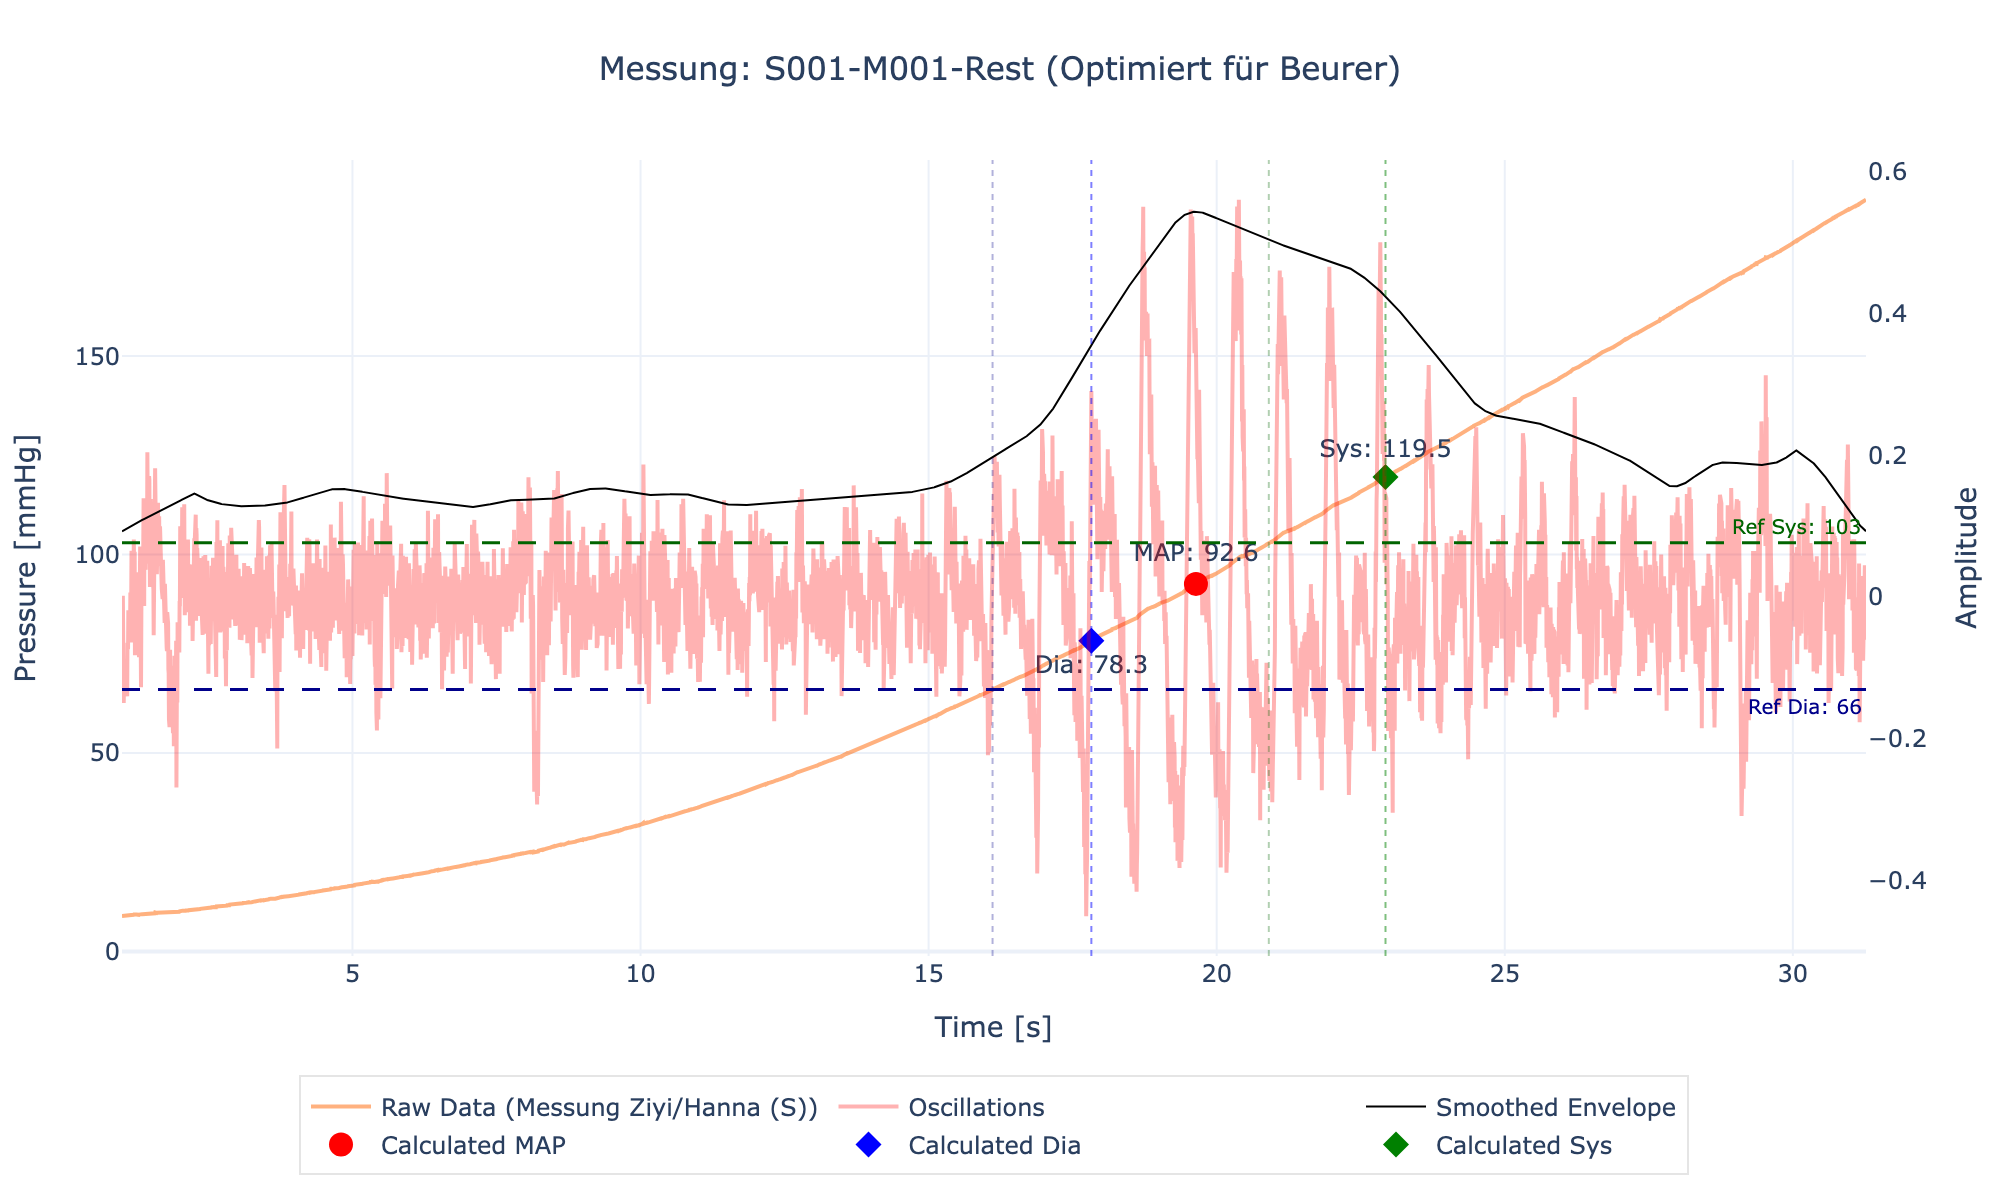
\includegraphics[width=\textwidth]{images/S001-M001-Rest_beurer.png}
        \caption{Optimiert für Beurer}
    \end{subfigure}
    \hfill
    \begin{subfigure}[b]{0.48\textwidth}
        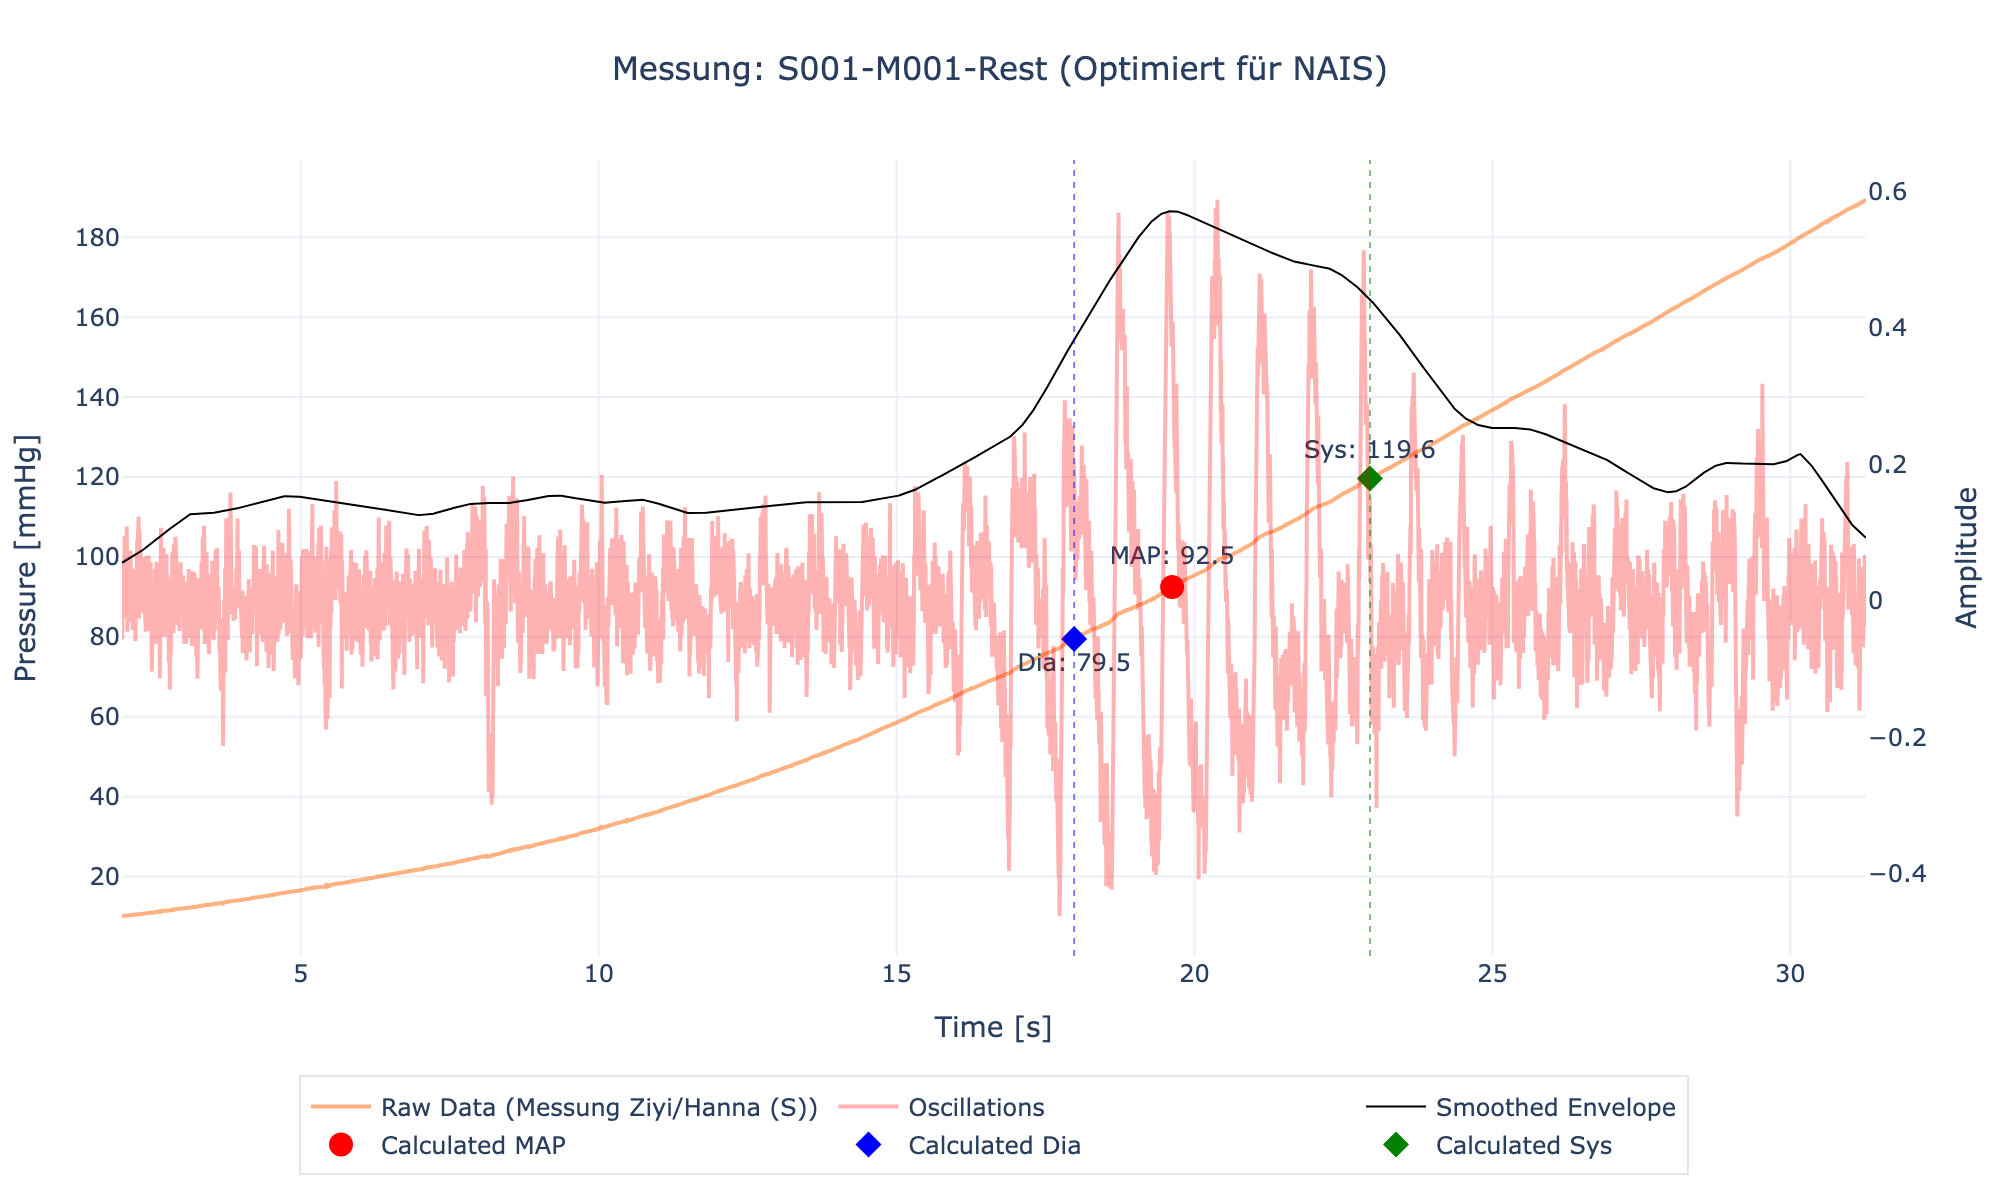
\includegraphics[width=\textwidth]{images/S001-M001-Rest_nais.png}
        \caption{Optimiert für NAIS}
    \end{subfigure}
    \caption{Einzelauswertung der Messung S001-M001-Rest mit verschiedenen Parametersätzen.}
\end{figure}
\newpage

\subsection*{Messung: S001-M002-Active}
\begin{figure}[H]
    \centering
    \begin{subfigure}[b]{0.8\textwidth}
        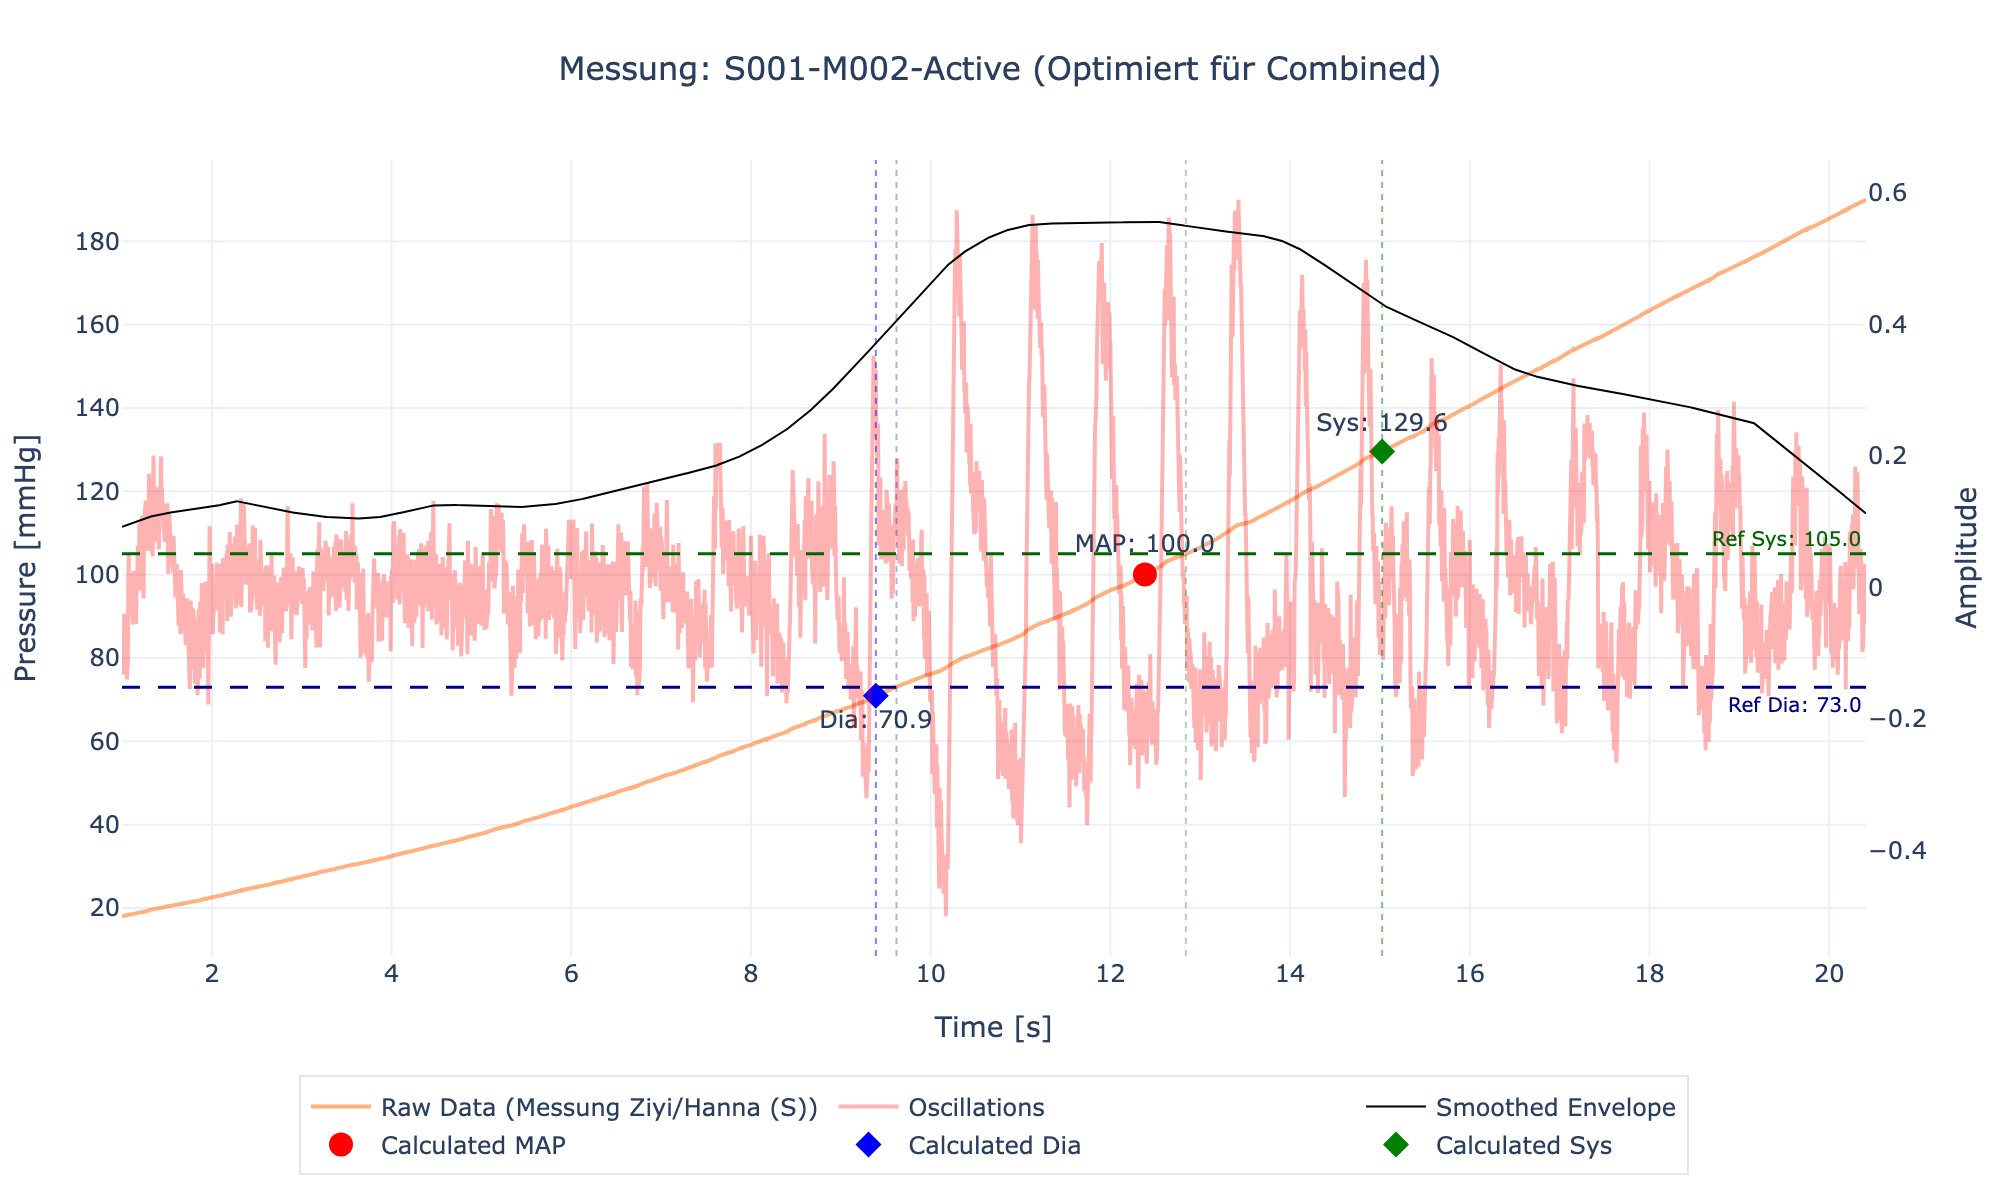
\includegraphics[width=\textwidth]{images/S001-M002-Active_combined.png}
        \caption{Optimiert für Beurer und NAIS (Kombiniert)}
    \end{subfigure} \\
    \begin{subfigure}[b]{0.48\textwidth}
        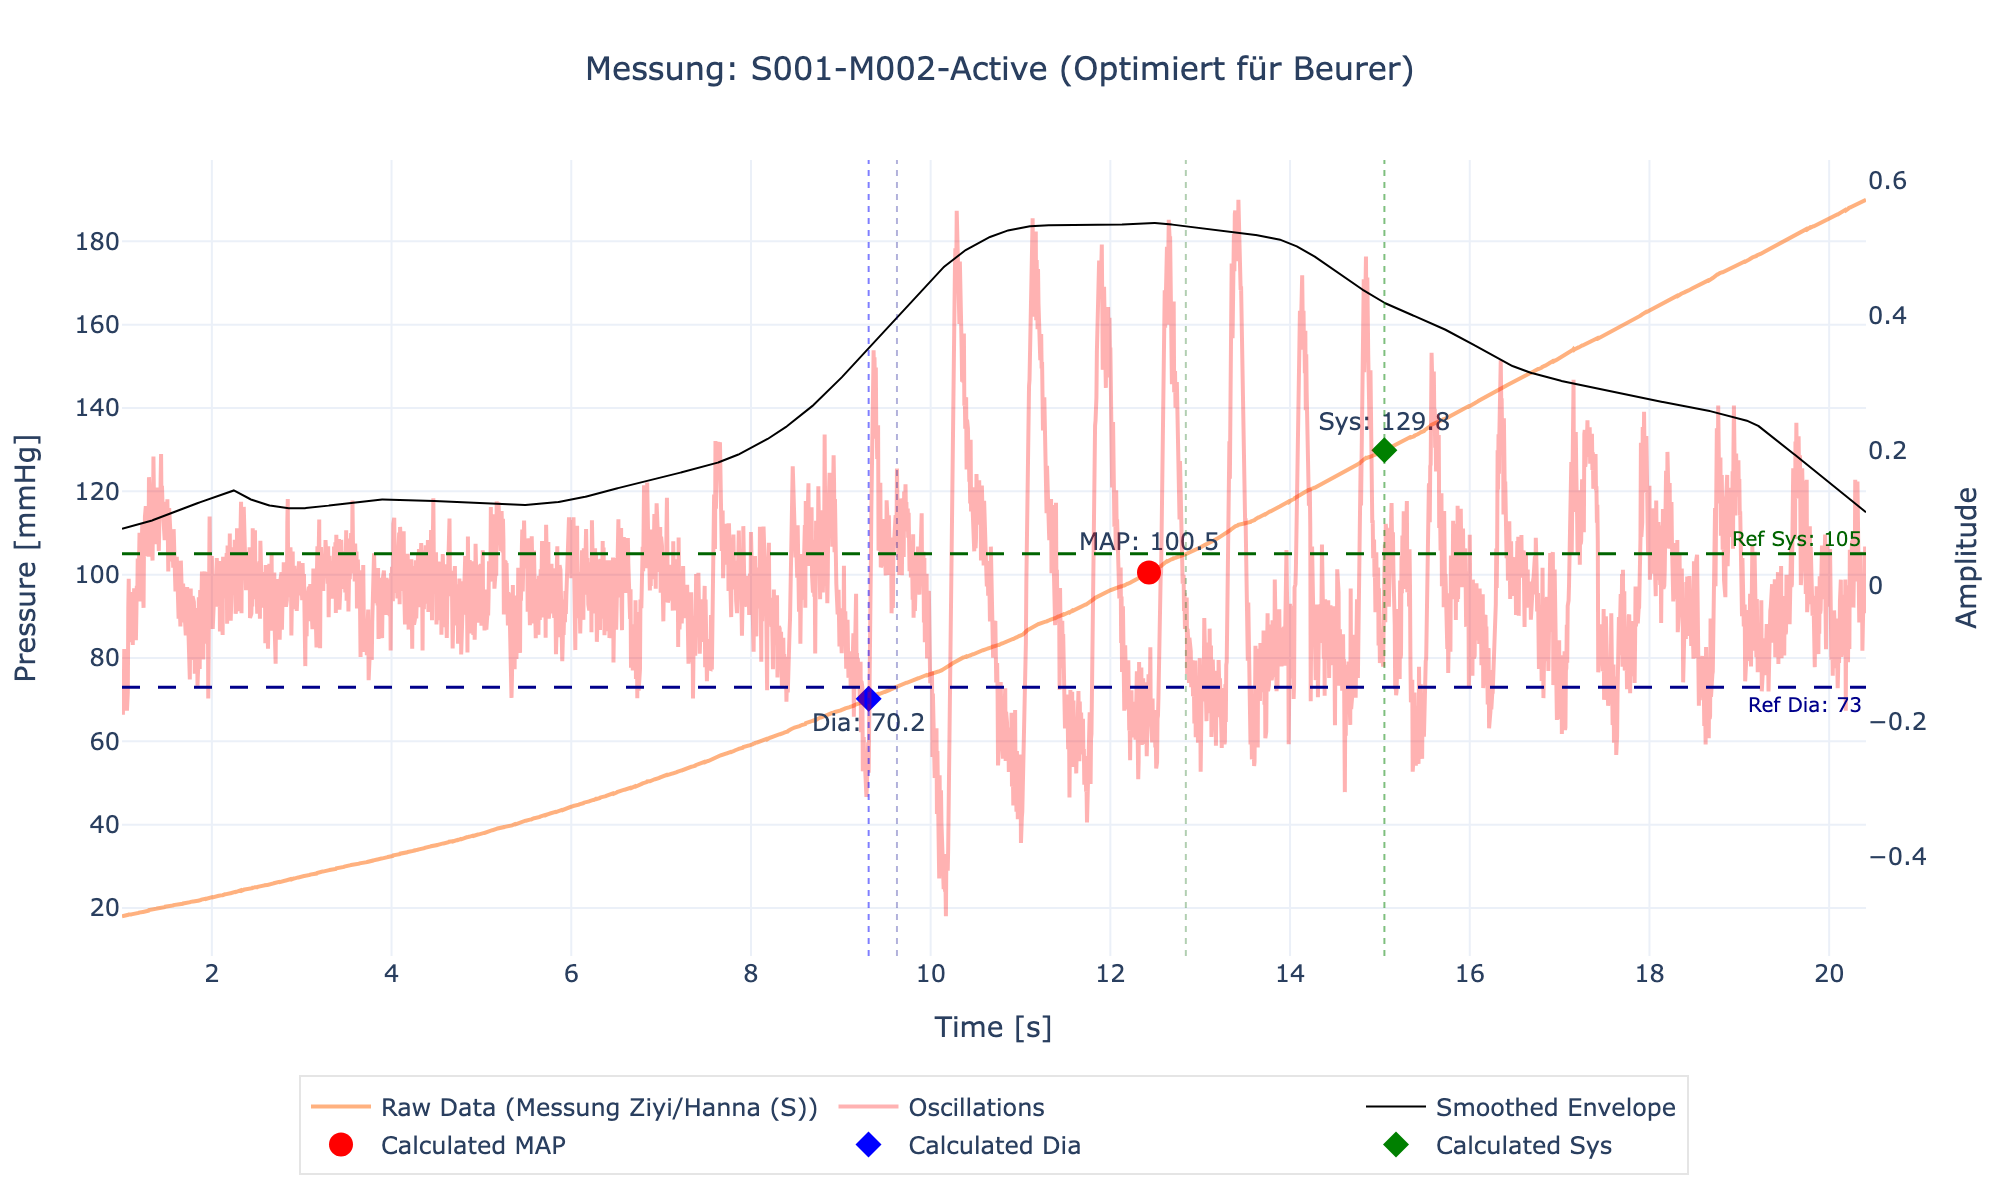
\includegraphics[width=\textwidth]{images/S001-M002-Active_beurer.png}
        \caption{Optimiert für Beurer}
    \end{subfigure}
    \hfill
    \begin{subfigure}[b]{0.48\textwidth}
        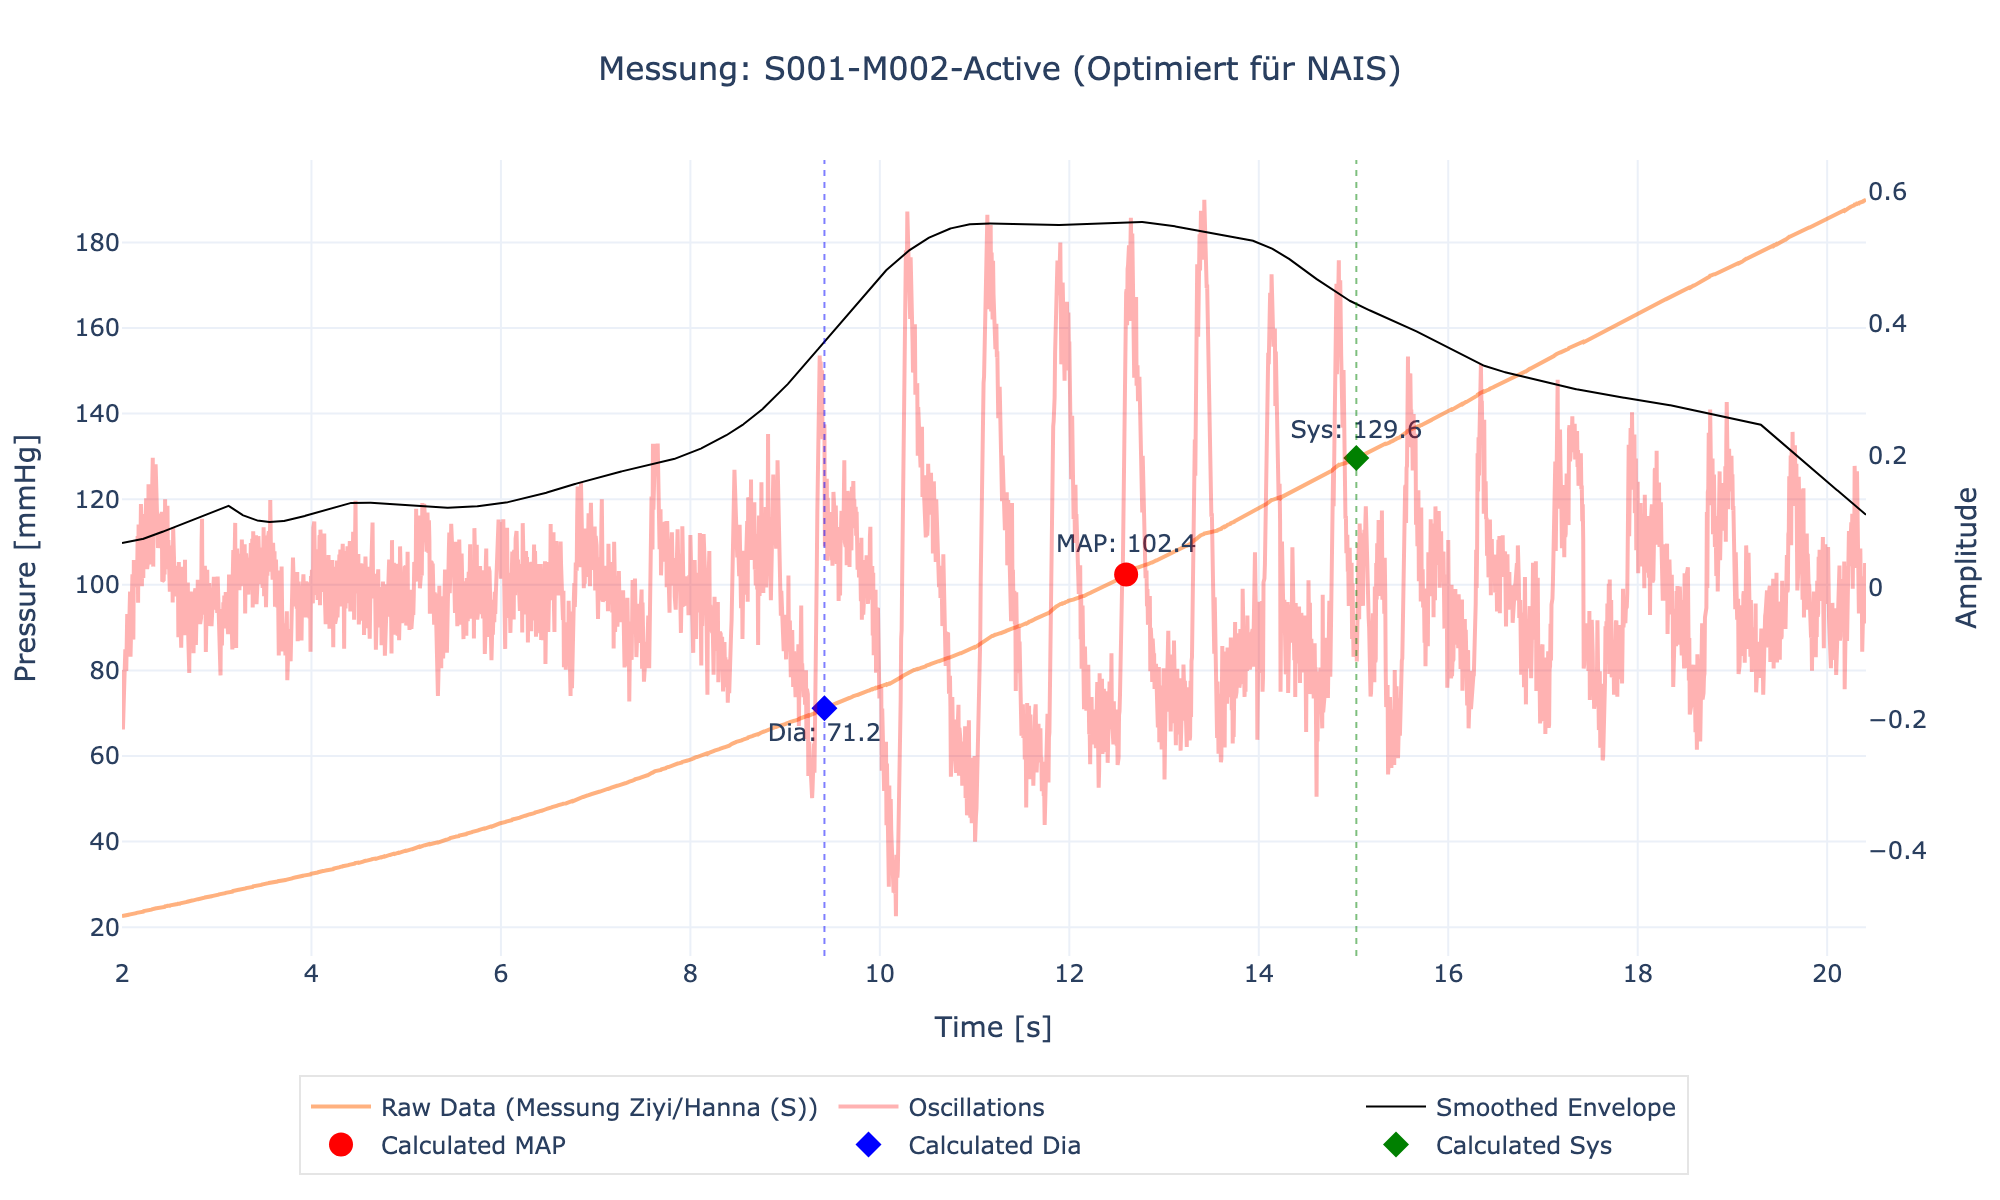
\includegraphics[width=\textwidth]{images/S001-M002-Active_nais.png}
        \caption{Optimiert für NAIS}
    \end{subfigure}
    \caption{Einzelauswertung der Messung S001-M002-Active mit verschiedenen Parametersätzen.}
\end{figure}
\newpage

\subsection*{Messung: S002-M001-Rest}
\begin{figure}[H]
    \centering
    \begin{subfigure}[b]{0.8\textwidth}
        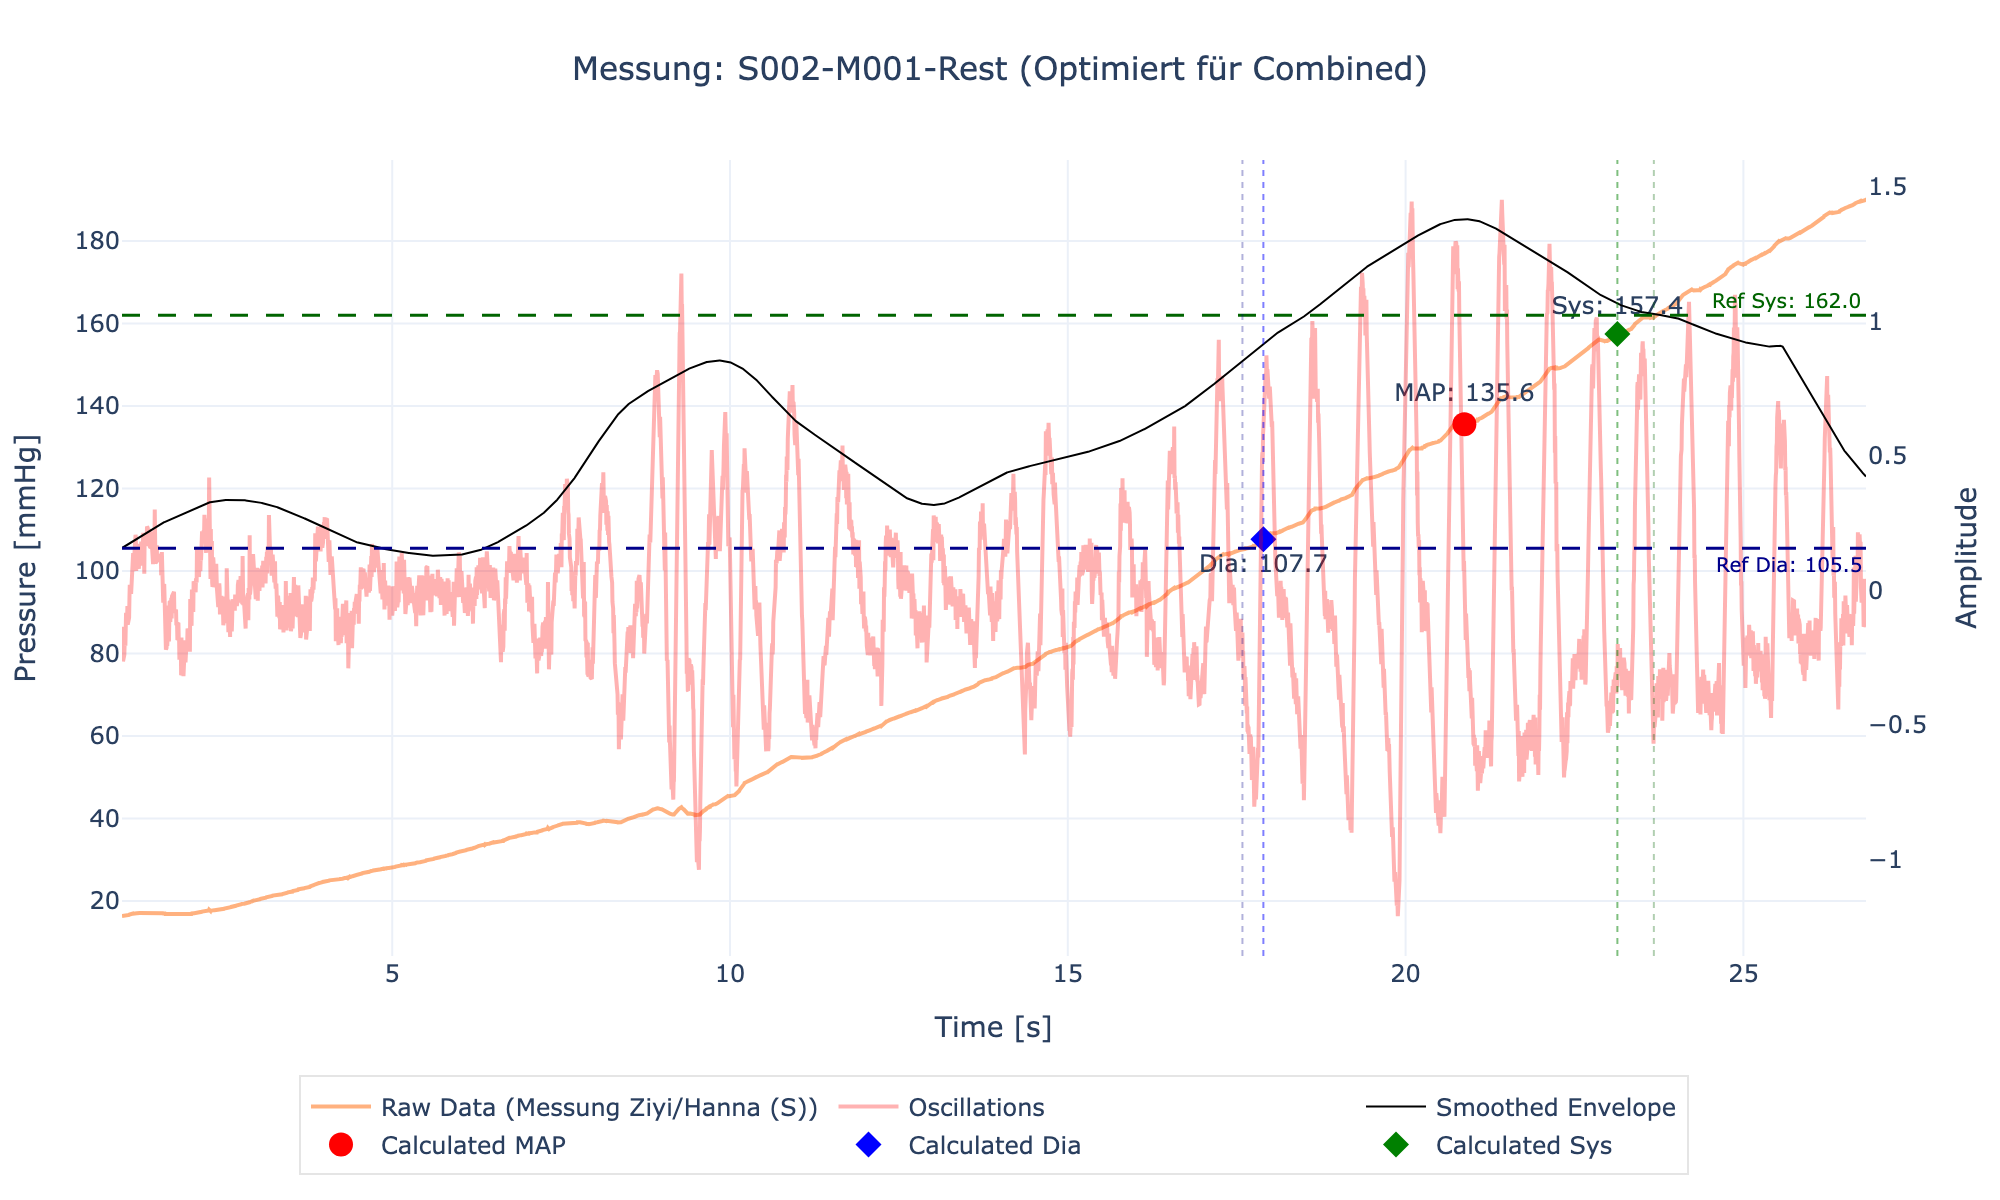
\includegraphics[width=\textwidth]{images/S002-M001-Rest_combined.png}
        \caption{Optimiert für Beurer und NAIS (Kombiniert)}
    \end{subfigure} \\
    \begin{subfigure}[b]{0.48\textwidth}
        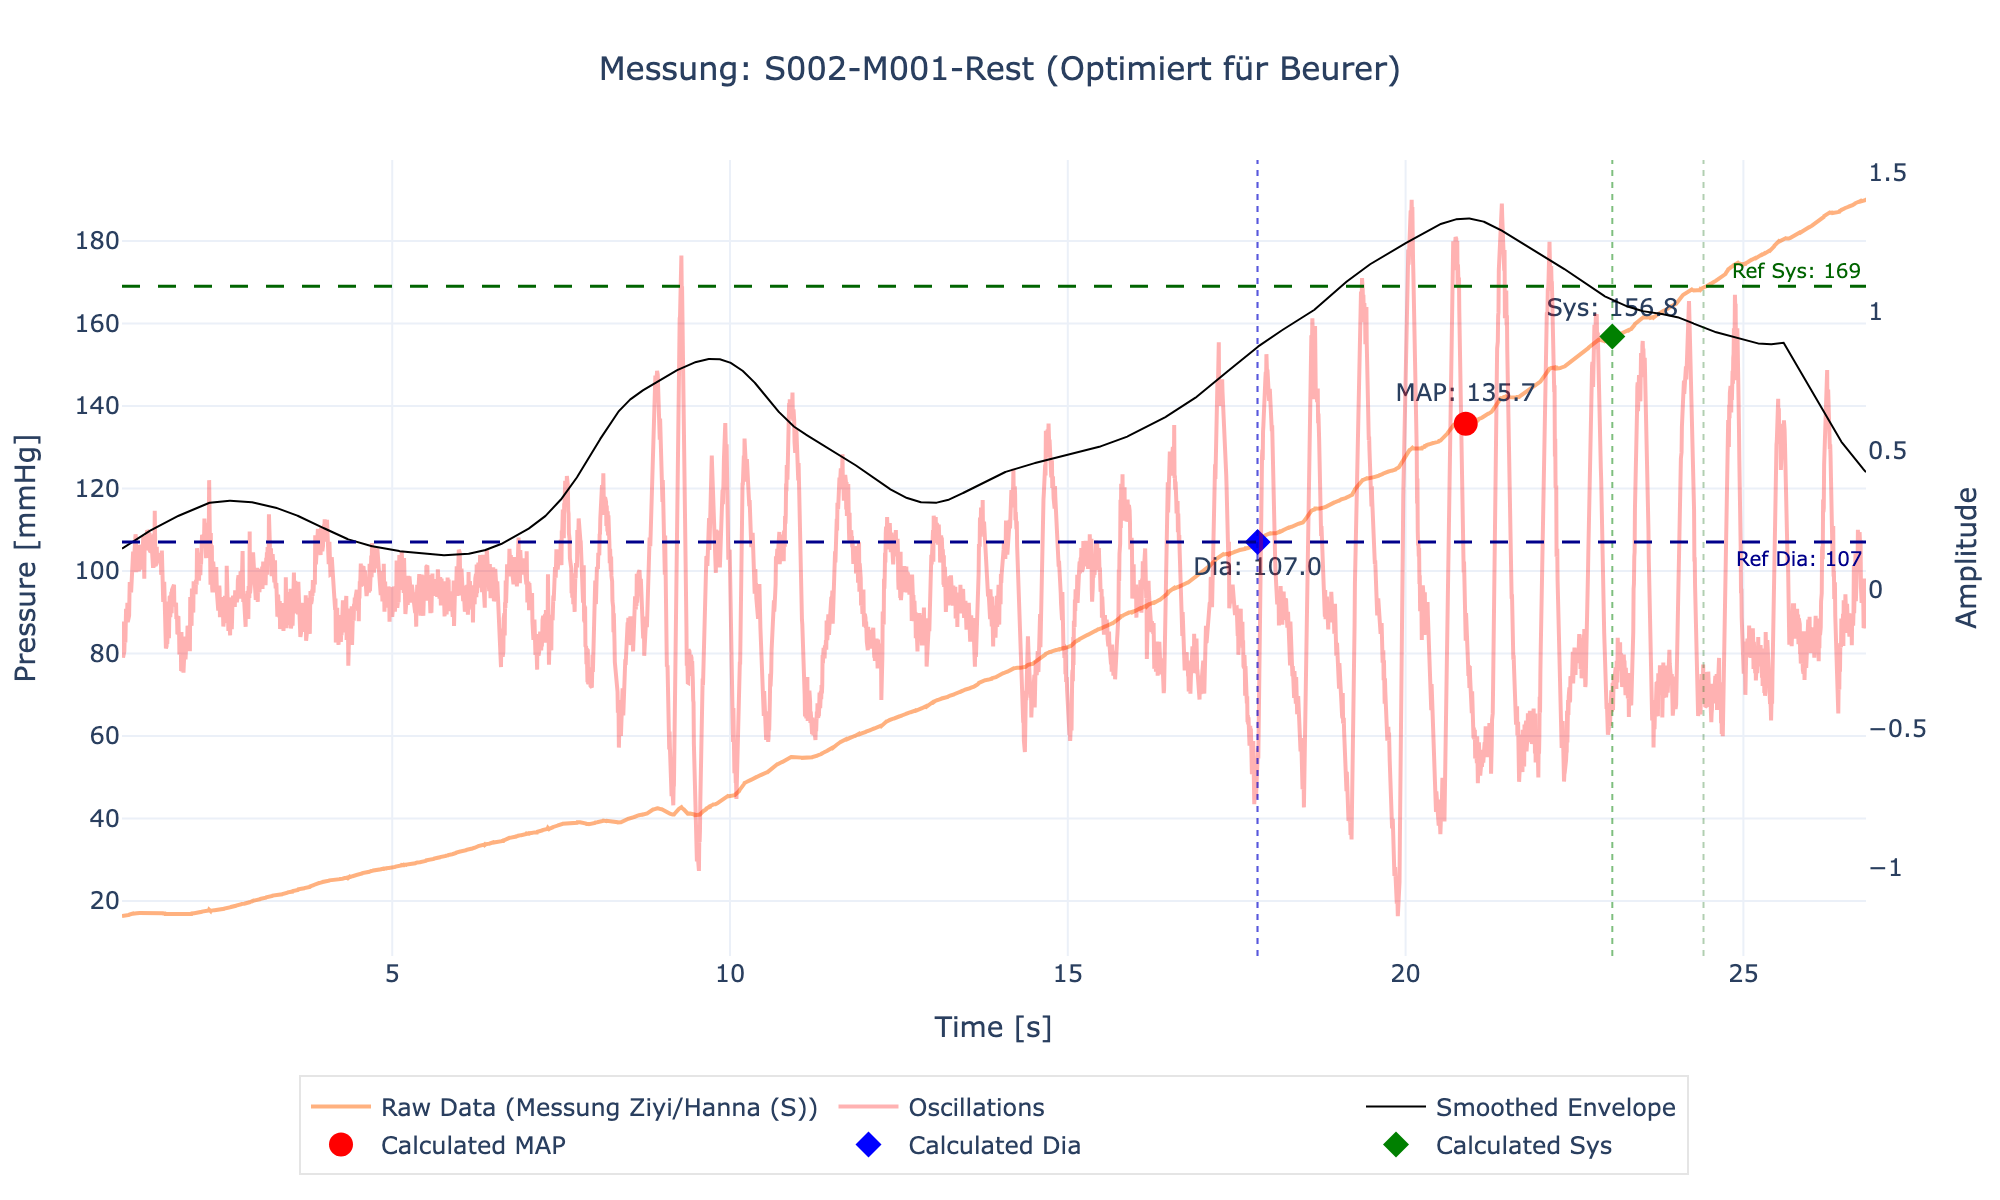
\includegraphics[width=\textwidth]{images/S002-M001-Rest_beurer.png}
        \caption{Optimiert für Beurer}
    \end{subfigure}
    \hfill
    \begin{subfigure}[b]{0.48\textwidth}
        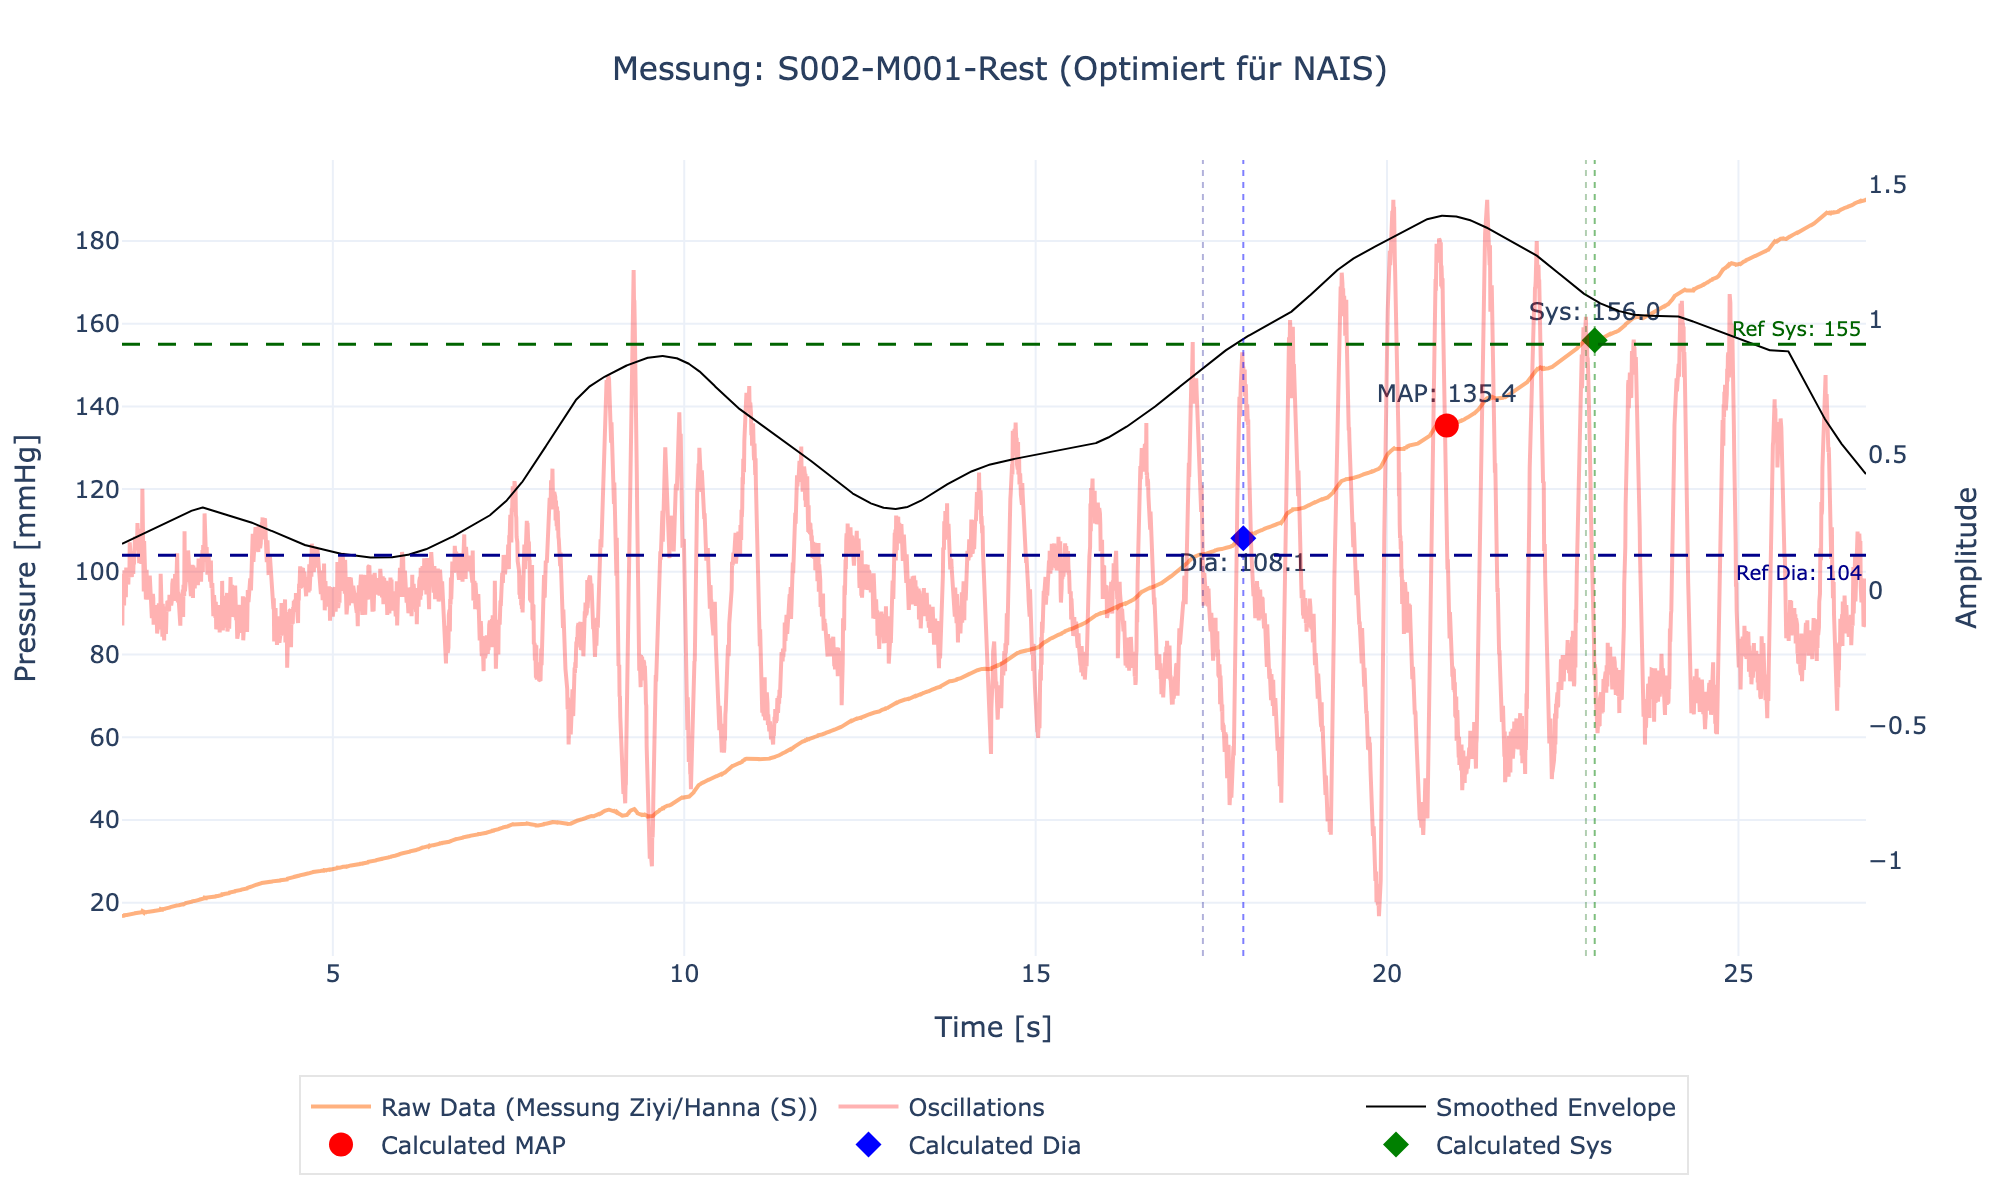
\includegraphics[width=\textwidth]{images/S002-M001-Rest_nais.png}
        \caption{Optimiert für NAIS}
    \end{subfigure}
    \caption{Einzelauswertung der Messung S002-M001-Rest mit verschiedenen Parametersätzen.}
\end{figure}
\newpage

\subsection*{Messung: S002-M002-Active}
\begin{figure}[H]
    \centering
    \begin{subfigure}[b]{0.8\textwidth}
        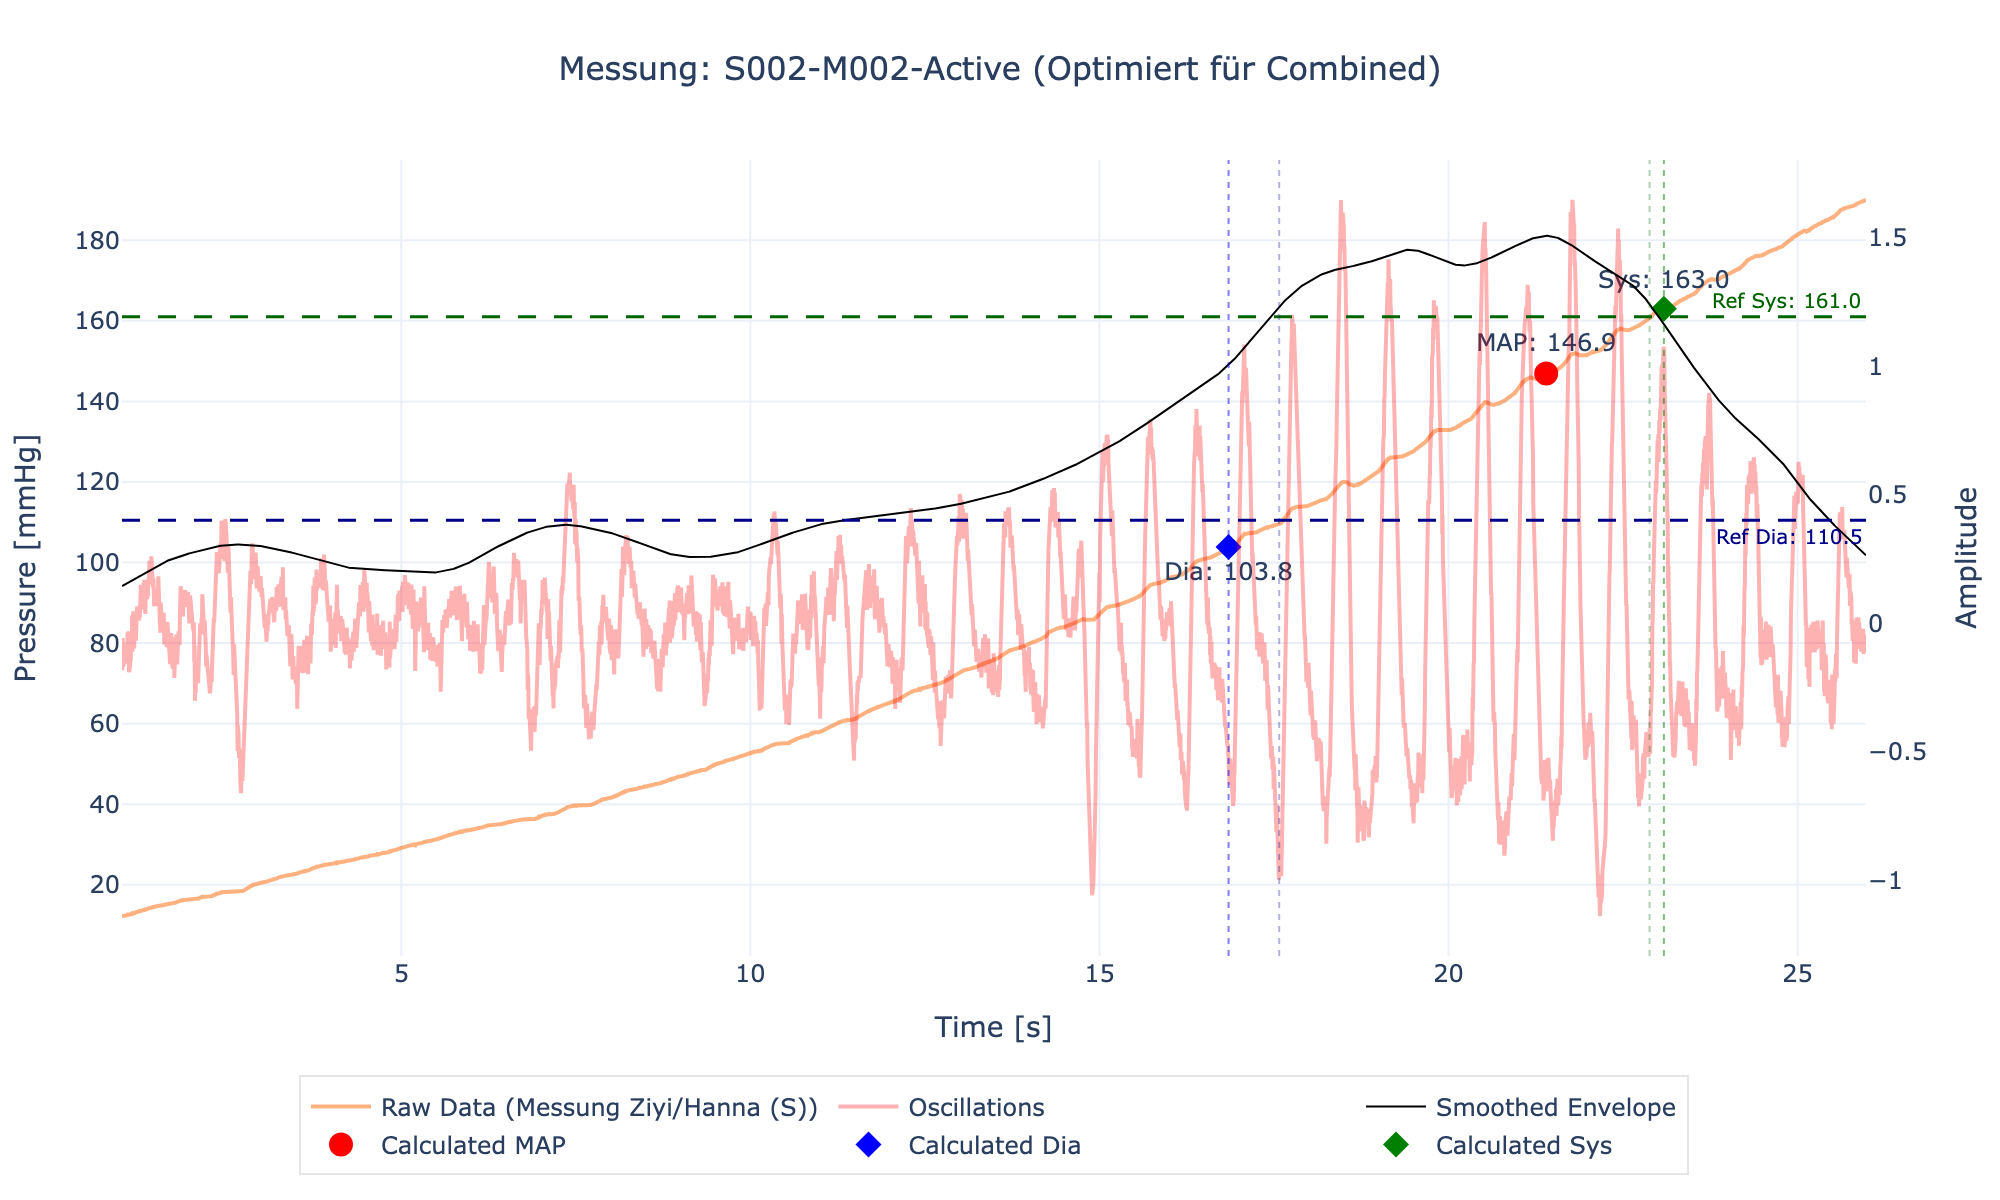
\includegraphics[width=\textwidth]{images/S002-M002-Active_combined.png}
        \caption{Optimiert für Beurer und NAIS (Kombiniert)}
    \end{subfigure} \\
    \begin{subfigure}[b]{0.48\textwidth}
        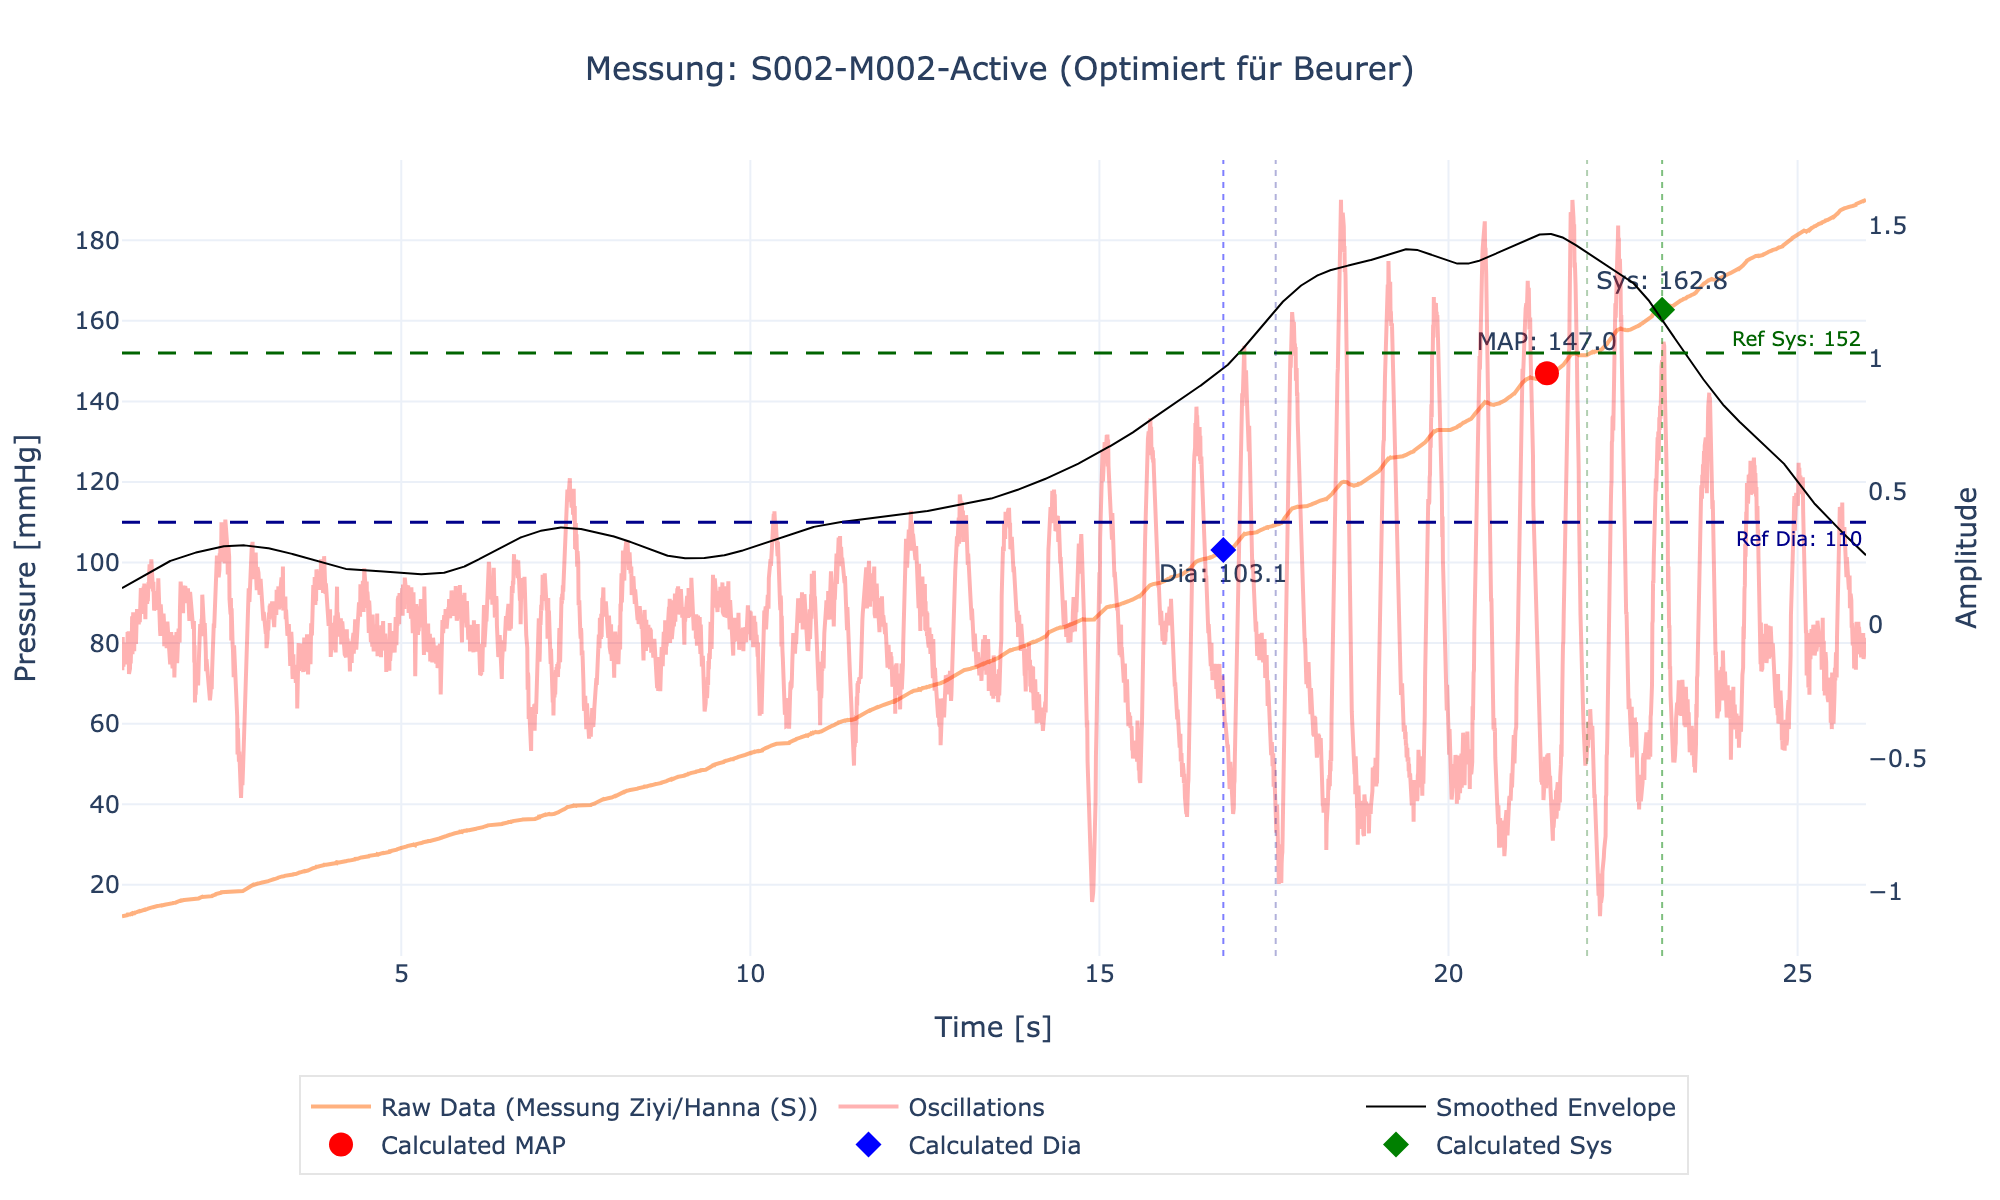
\includegraphics[width=\textwidth]{images/S002-M002-Active_beurer.png}
        \caption{Optimiert für Beurer}
    \end{subfigure}
    \hfill
    \begin{subfigure}[b]{0.48\textwidth}
        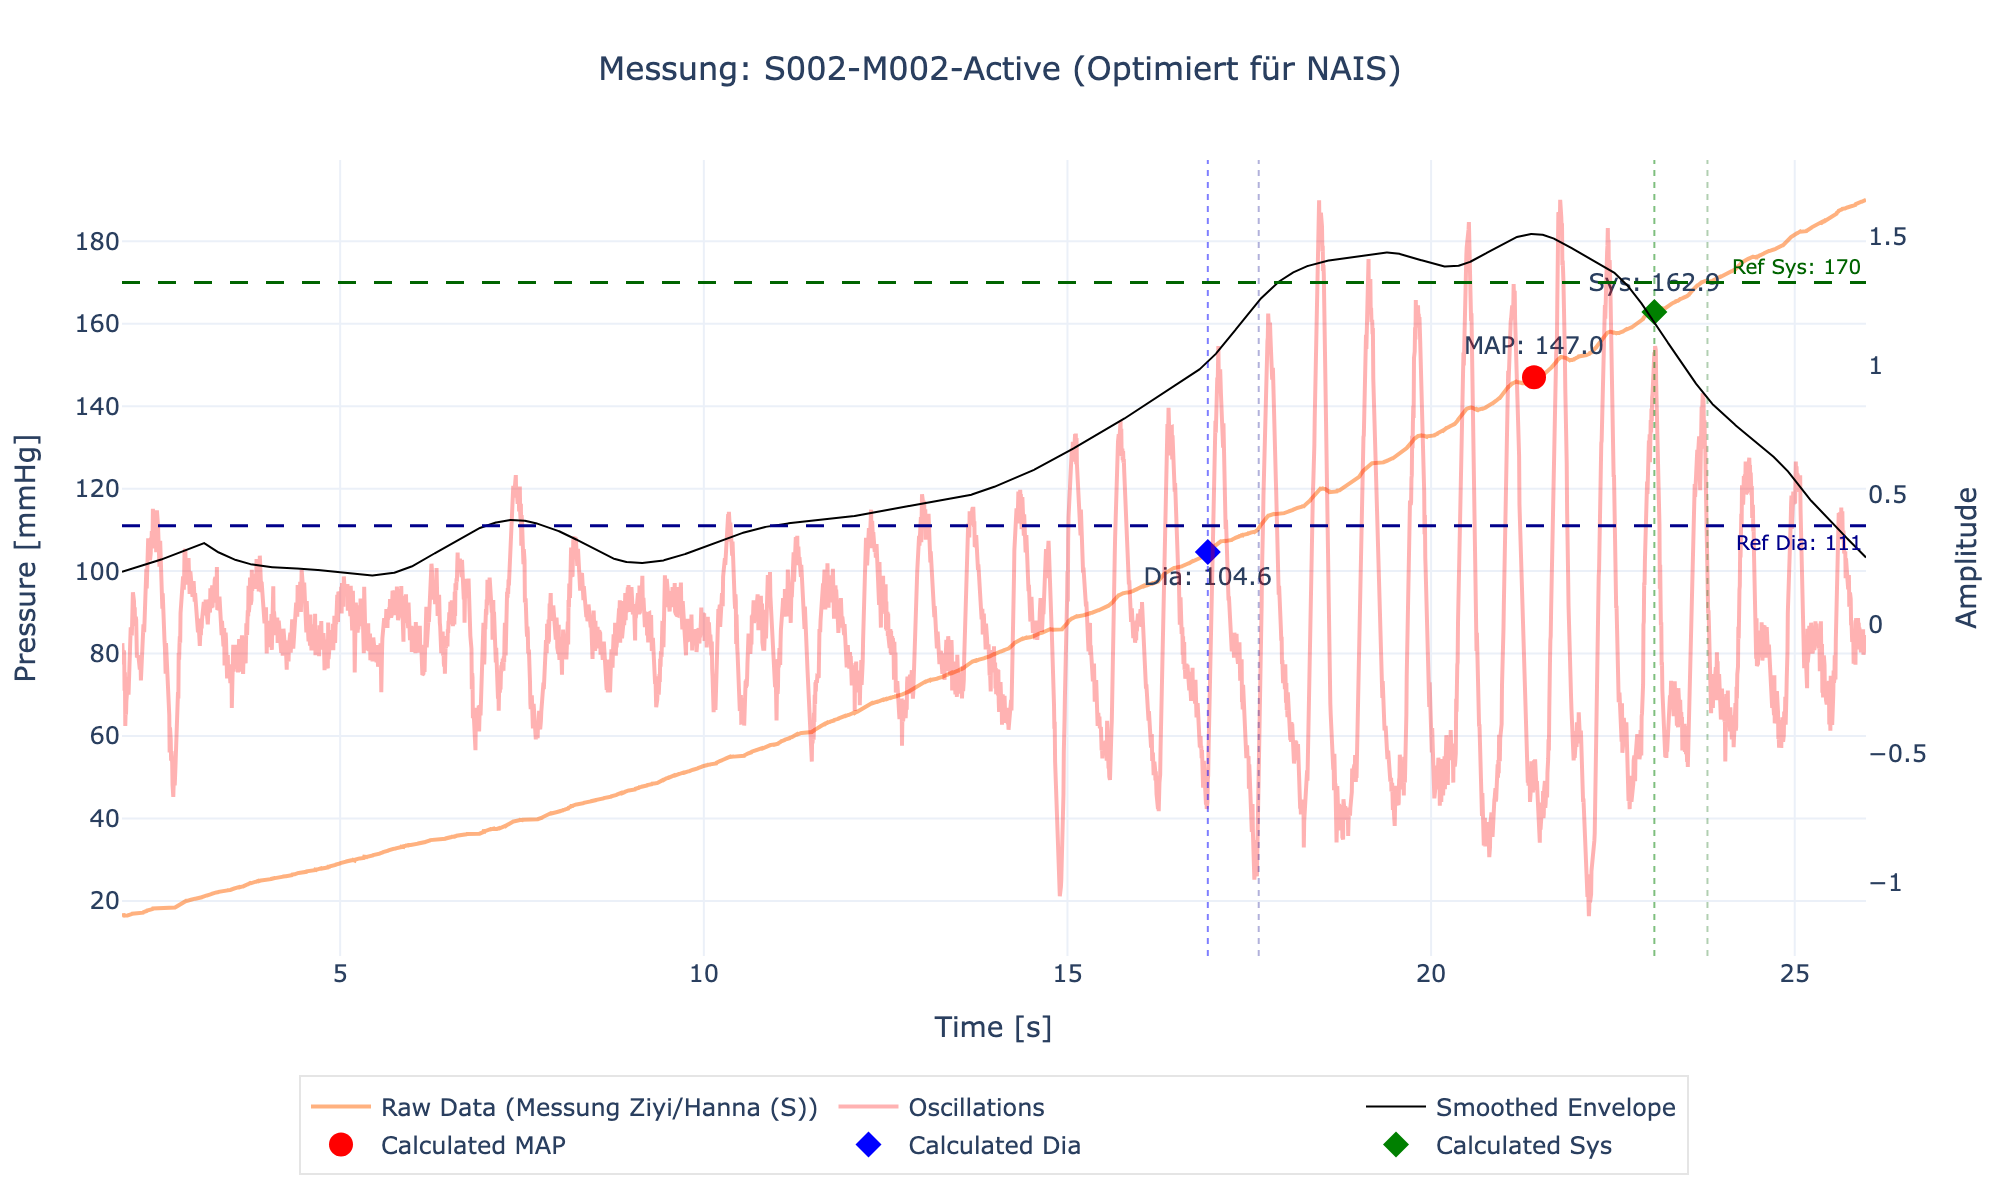
\includegraphics[width=\textwidth]{images/S002-M002-Active_nais.png}
        \caption{Optimiert für NAIS}
    \end{subfigure}
    \caption{Einzelauswertung der Messung S002-M002-Active mit verschiedenen Parametersätzen.}
\end{figure}
\newpage

\subsection*{Messung: S003-M001-Rest}
\begin{figure}[H]
    \centering
    \begin{subfigure}[b]{0.8\textwidth}
        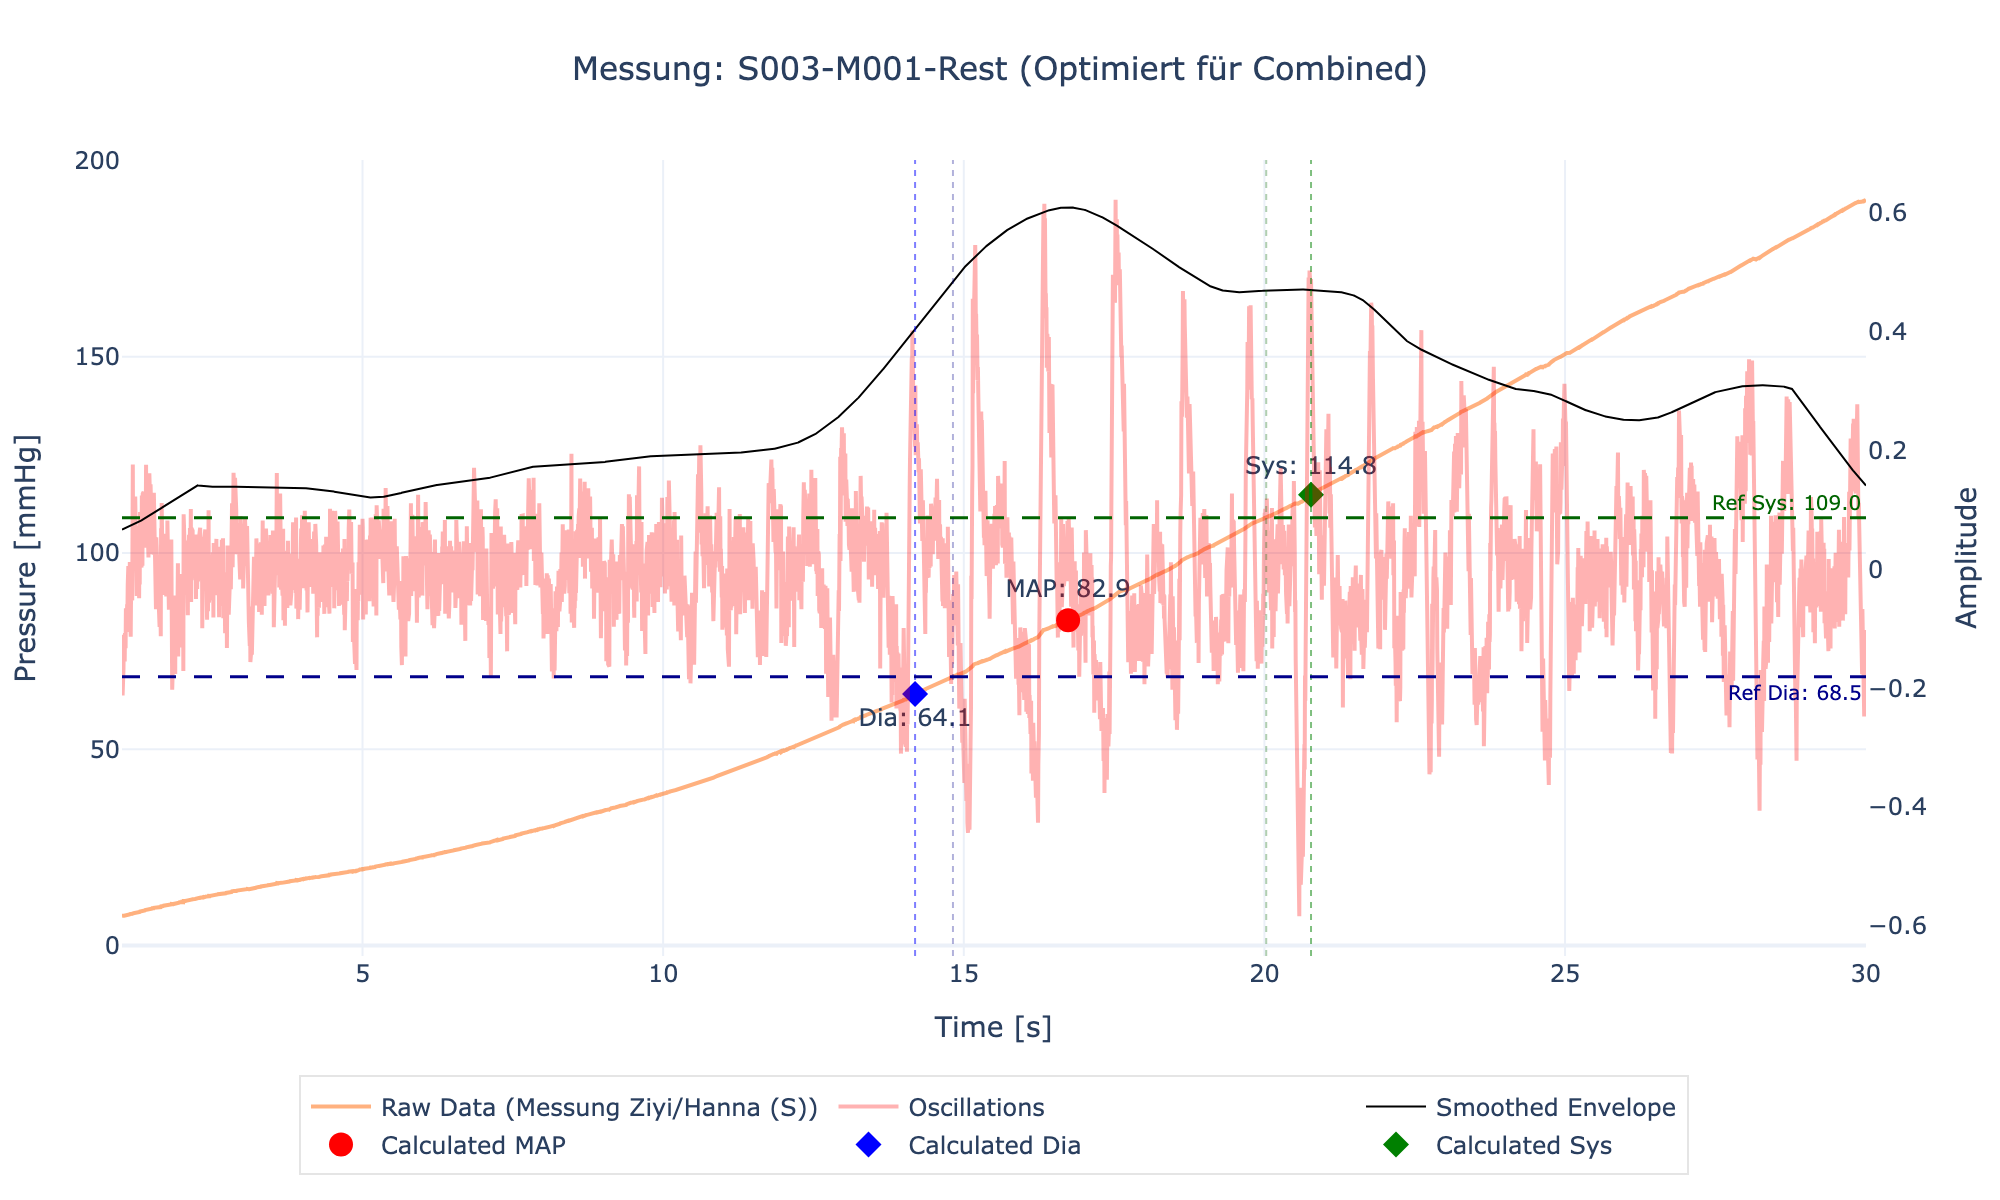
\includegraphics[width=\textwidth]{images/S003-M001-Rest_combined.png}
        \caption{Optimiert für Beurer und NAIS (Kombiniert)}
    \end{subfigure} \\
    \begin{subfigure}[b]{0.48\textwidth}
        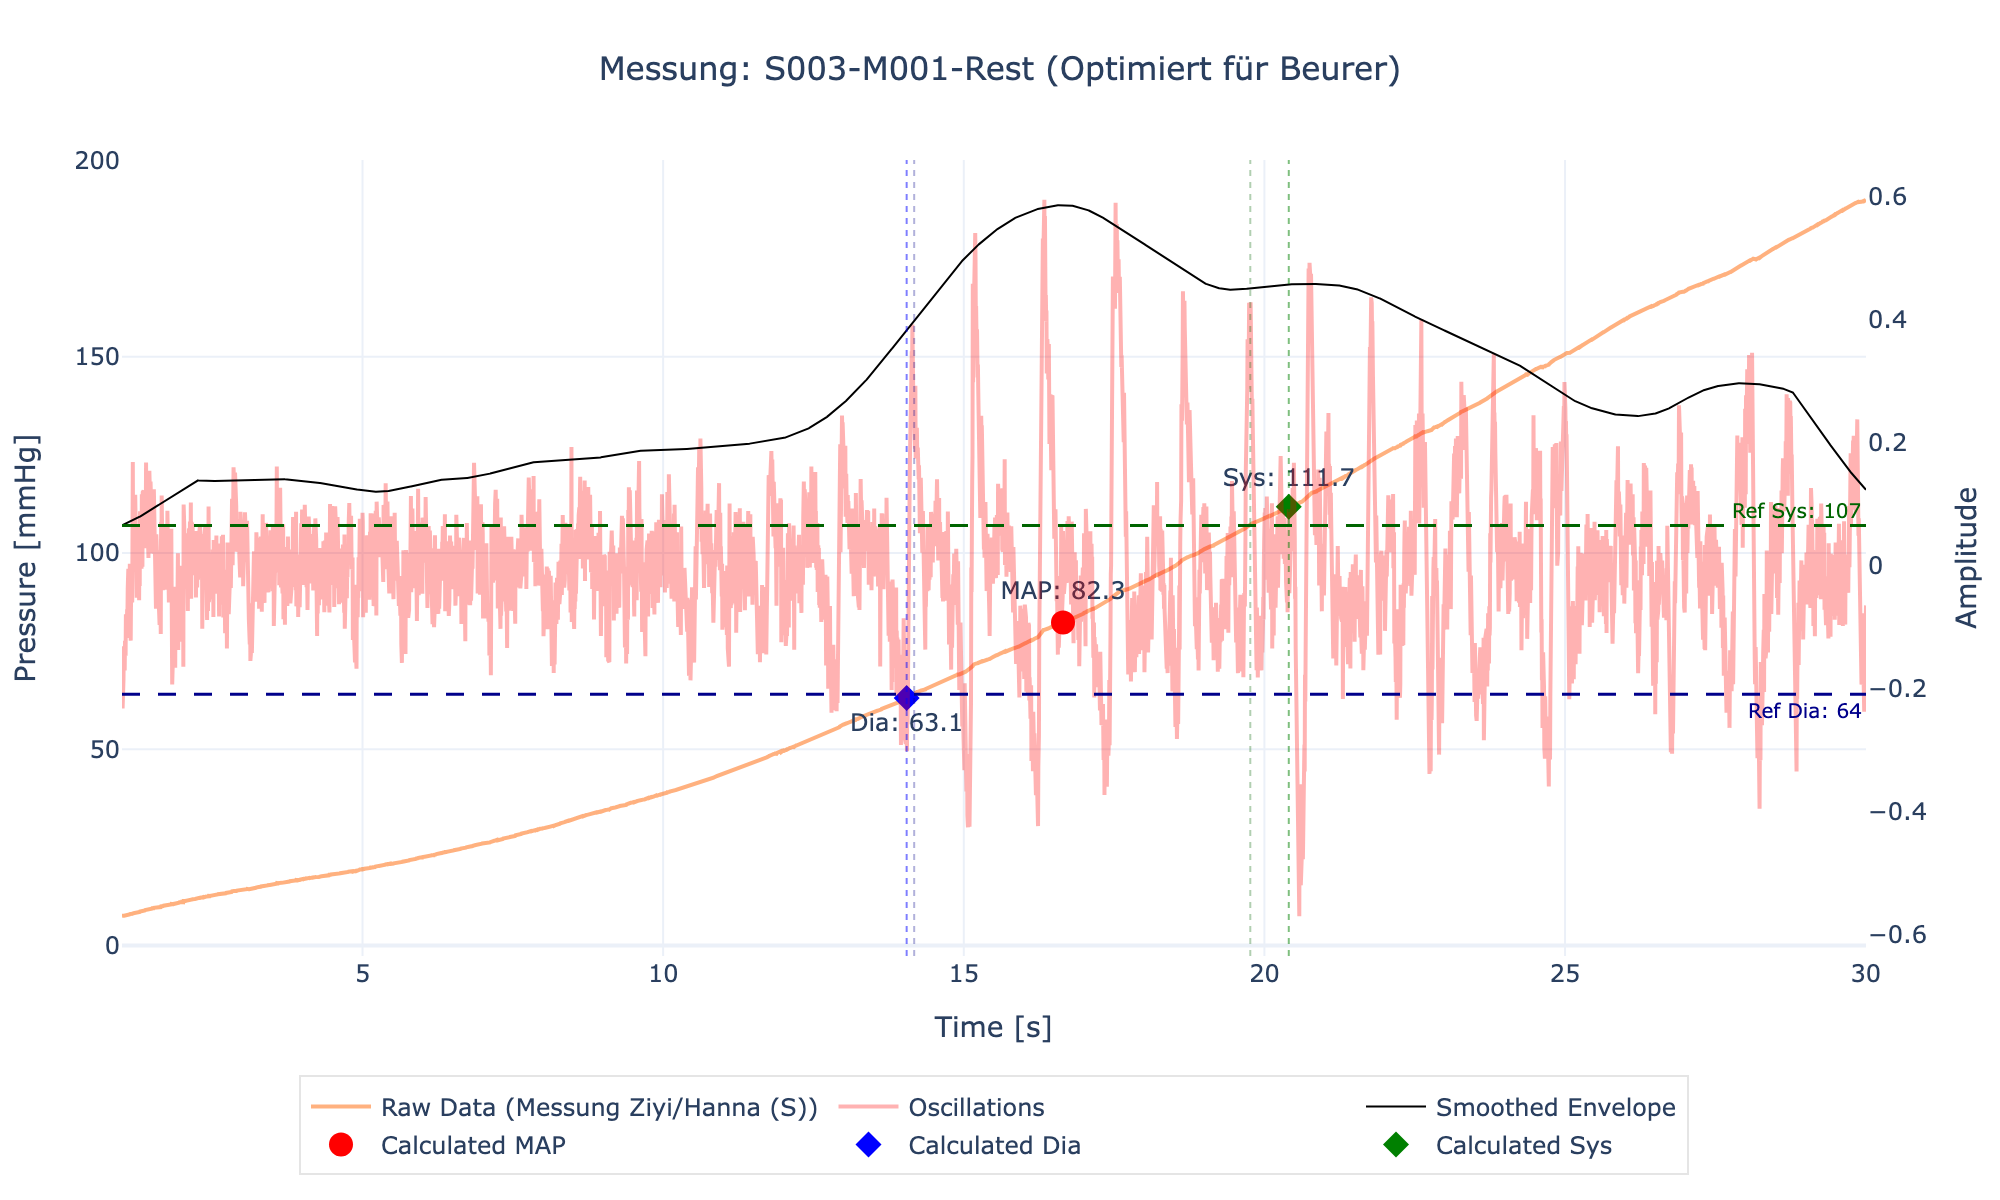
\includegraphics[width=\textwidth]{images/S003-M001-Rest_beurer.png}
        \caption{Optimiert für Beurer}
    \end{subfigure}
    \hfill
    \begin{subfigure}[b]{0.48\textwidth}
        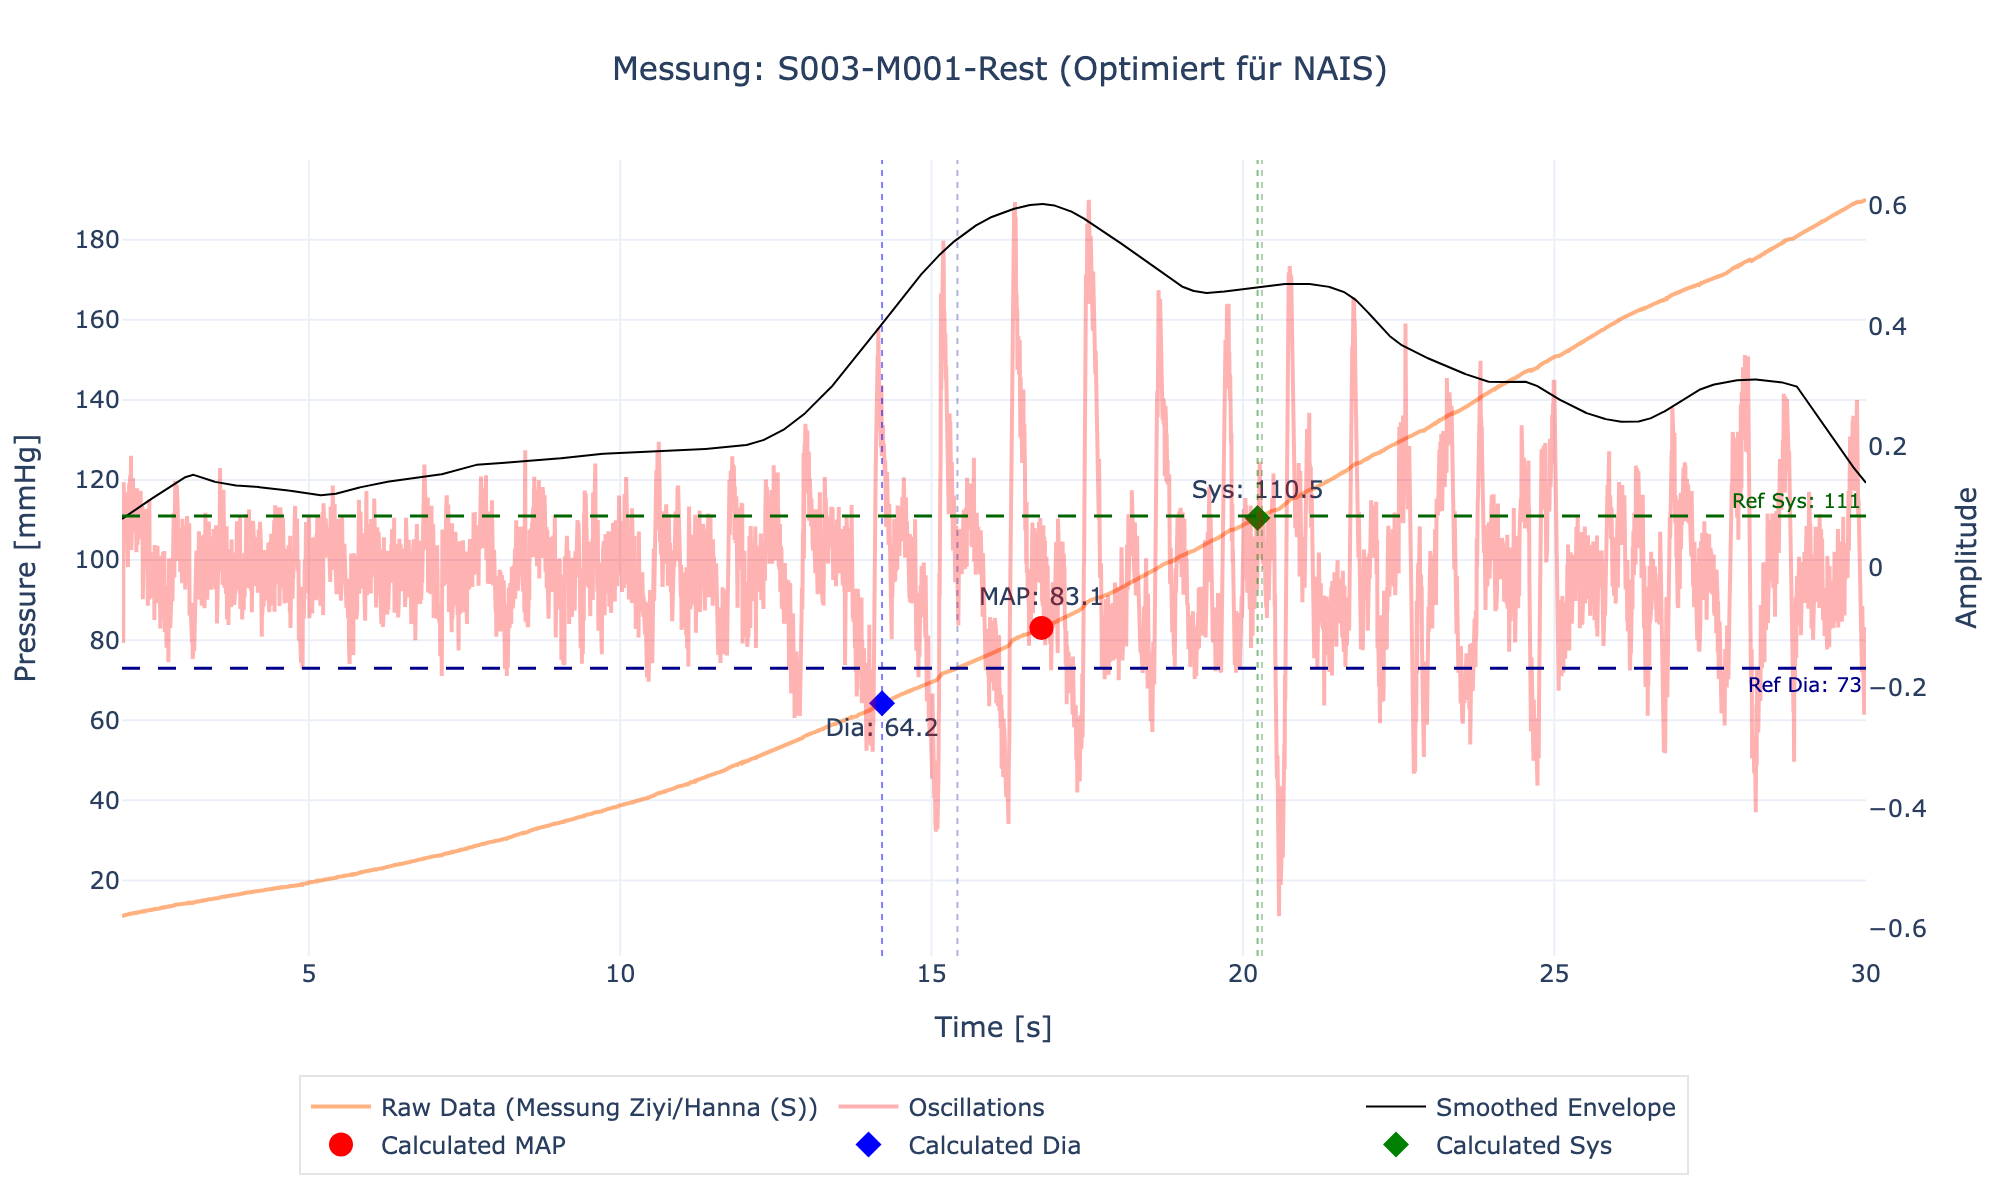
\includegraphics[width=\textwidth]{images/S003-M001-Rest_nais.png}
        \caption{Optimiert für NAIS}
    \end{subfigure}
    \caption{Einzelauswertung der Messung S003-M001-Rest mit verschiedenen Parametersätzen.}
\end{figure}
\newpage

\subsection*{Messung: S003-M002-Active}
\begin{figure}[H]
    \centering
    \begin{subfigure}[b]{0.8\textwidth}
        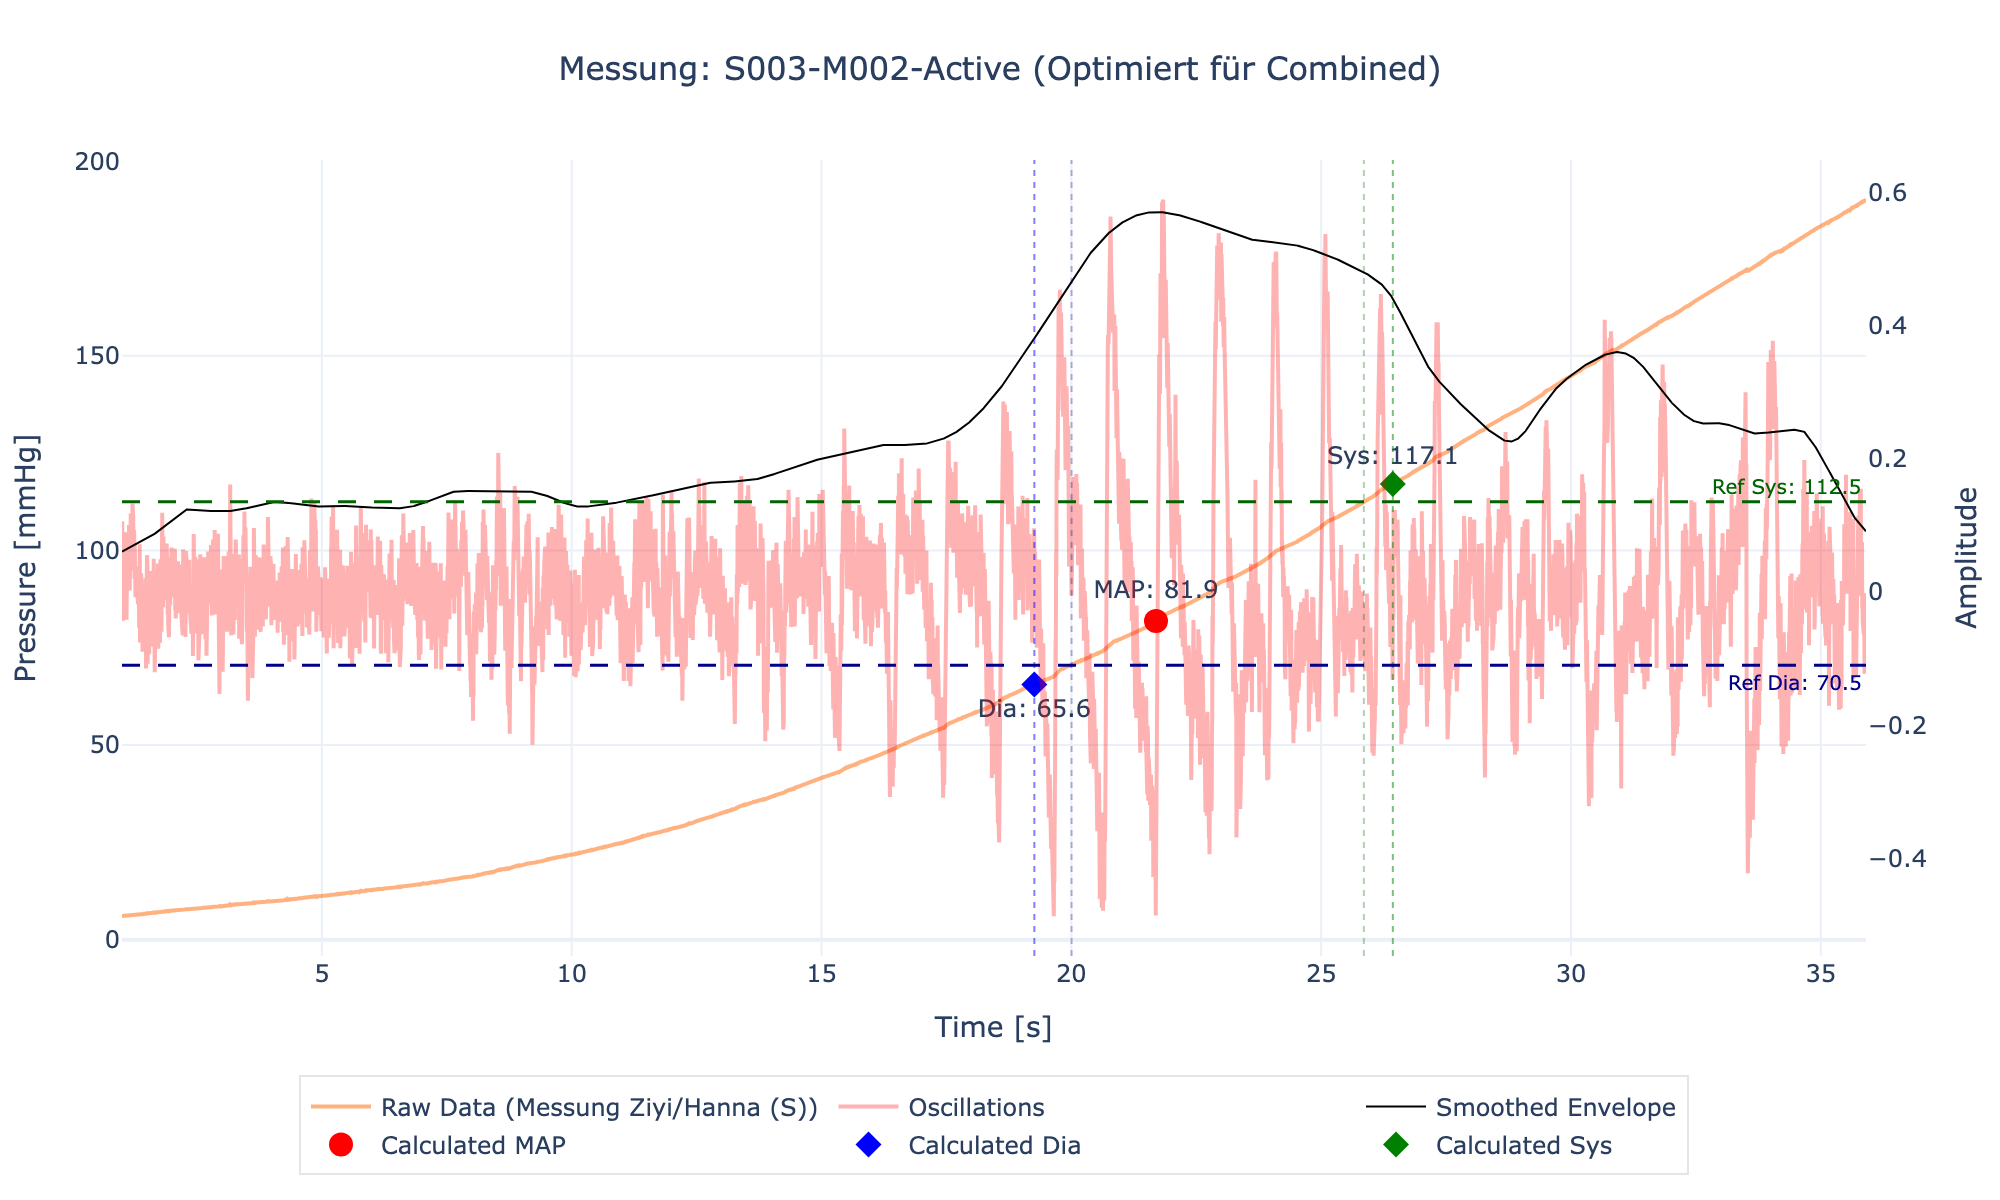
\includegraphics[width=\textwidth]{images/S003-M002-Active_combined.png}
        \caption{Optimiert für Beurer und NAIS (Kombiniert)}
    \end{subfigure} \\
    \begin{subfigure}[b]{0.48\textwidth}
        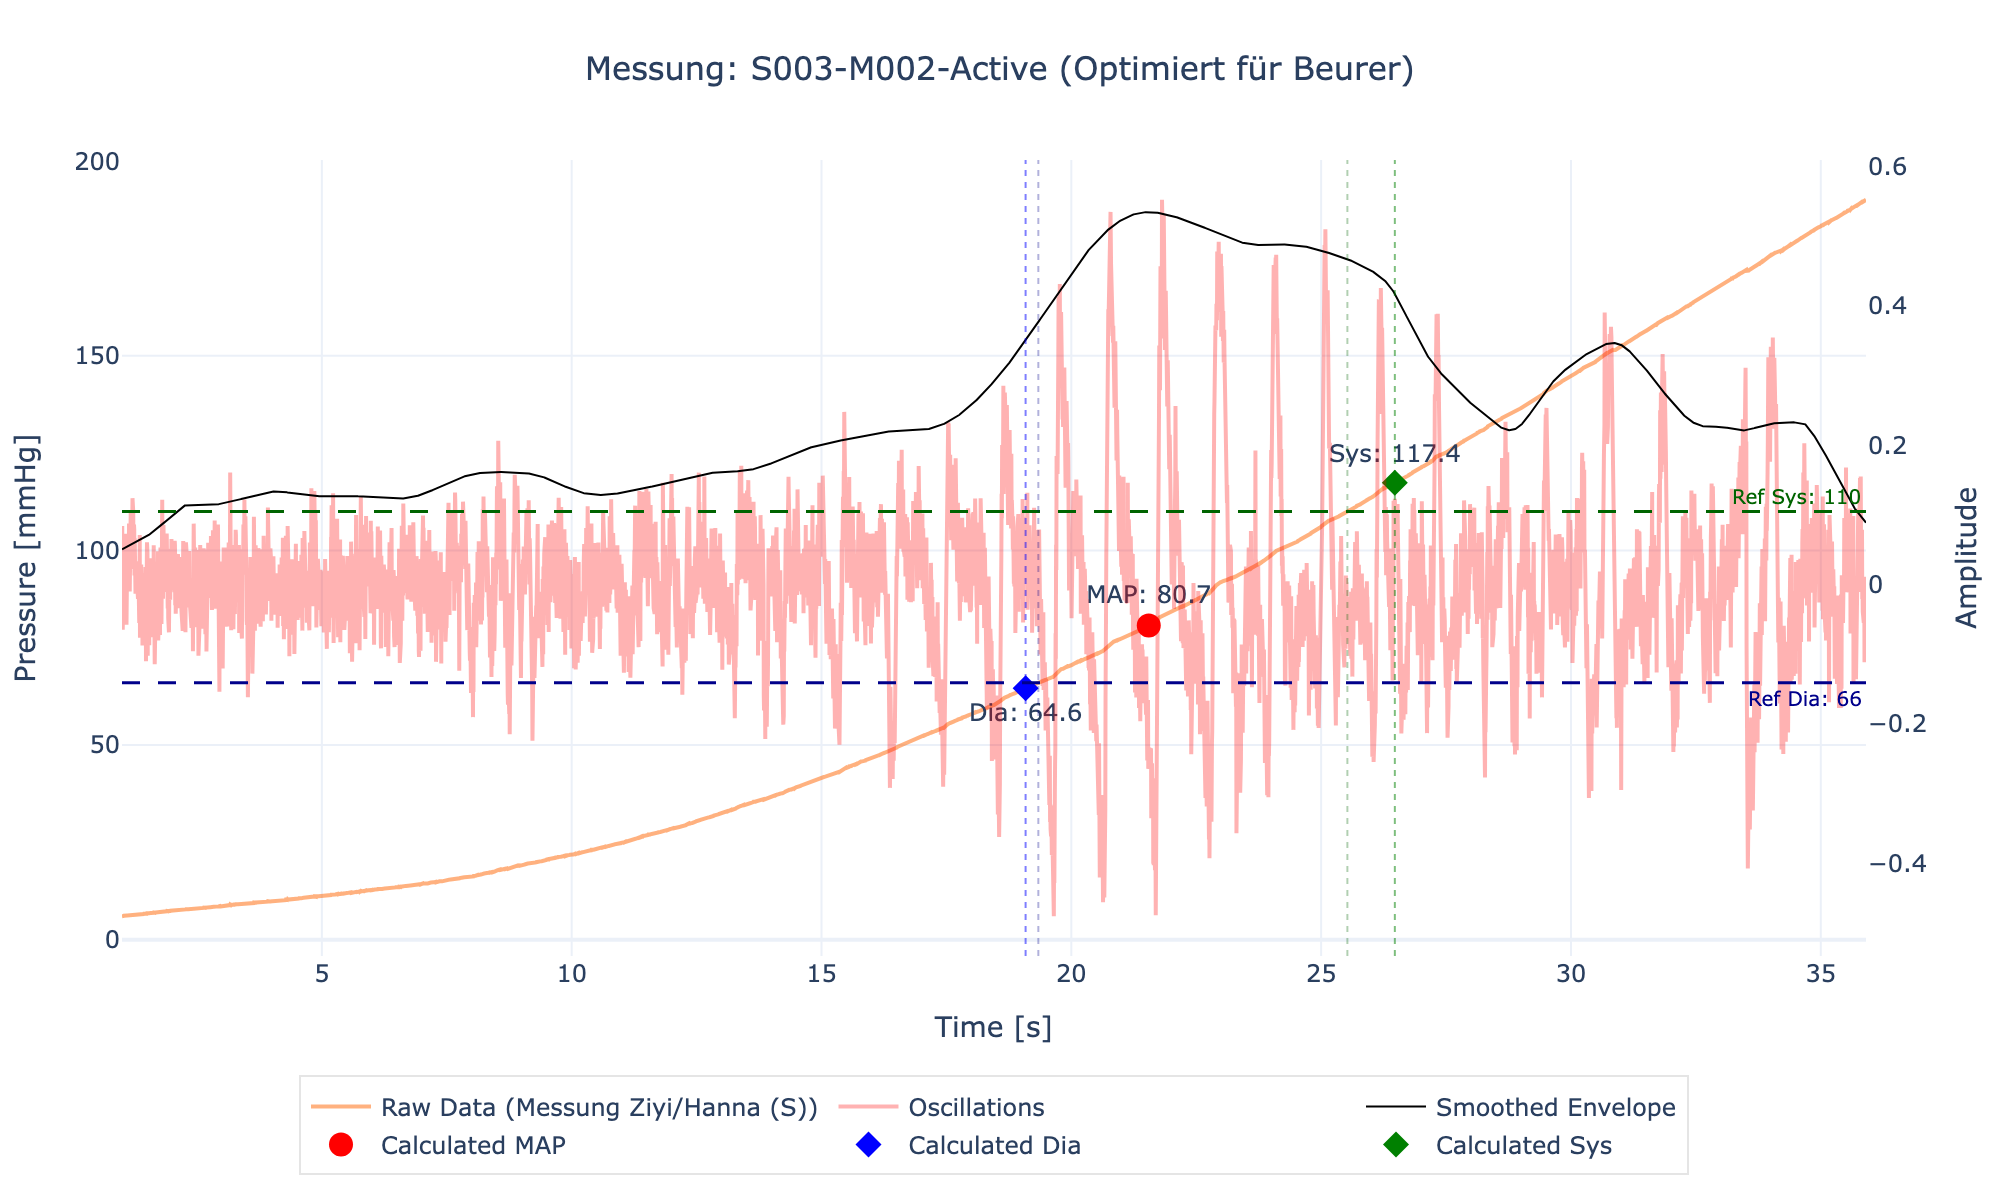
\includegraphics[width=\textwidth]{images/S003-M002-Active_beurer.png}
        \caption{Optimiert für Beurer}
    \end{subfigure}
    \hfill
    \begin{subfigure}[b]{0.48\textwidth}
        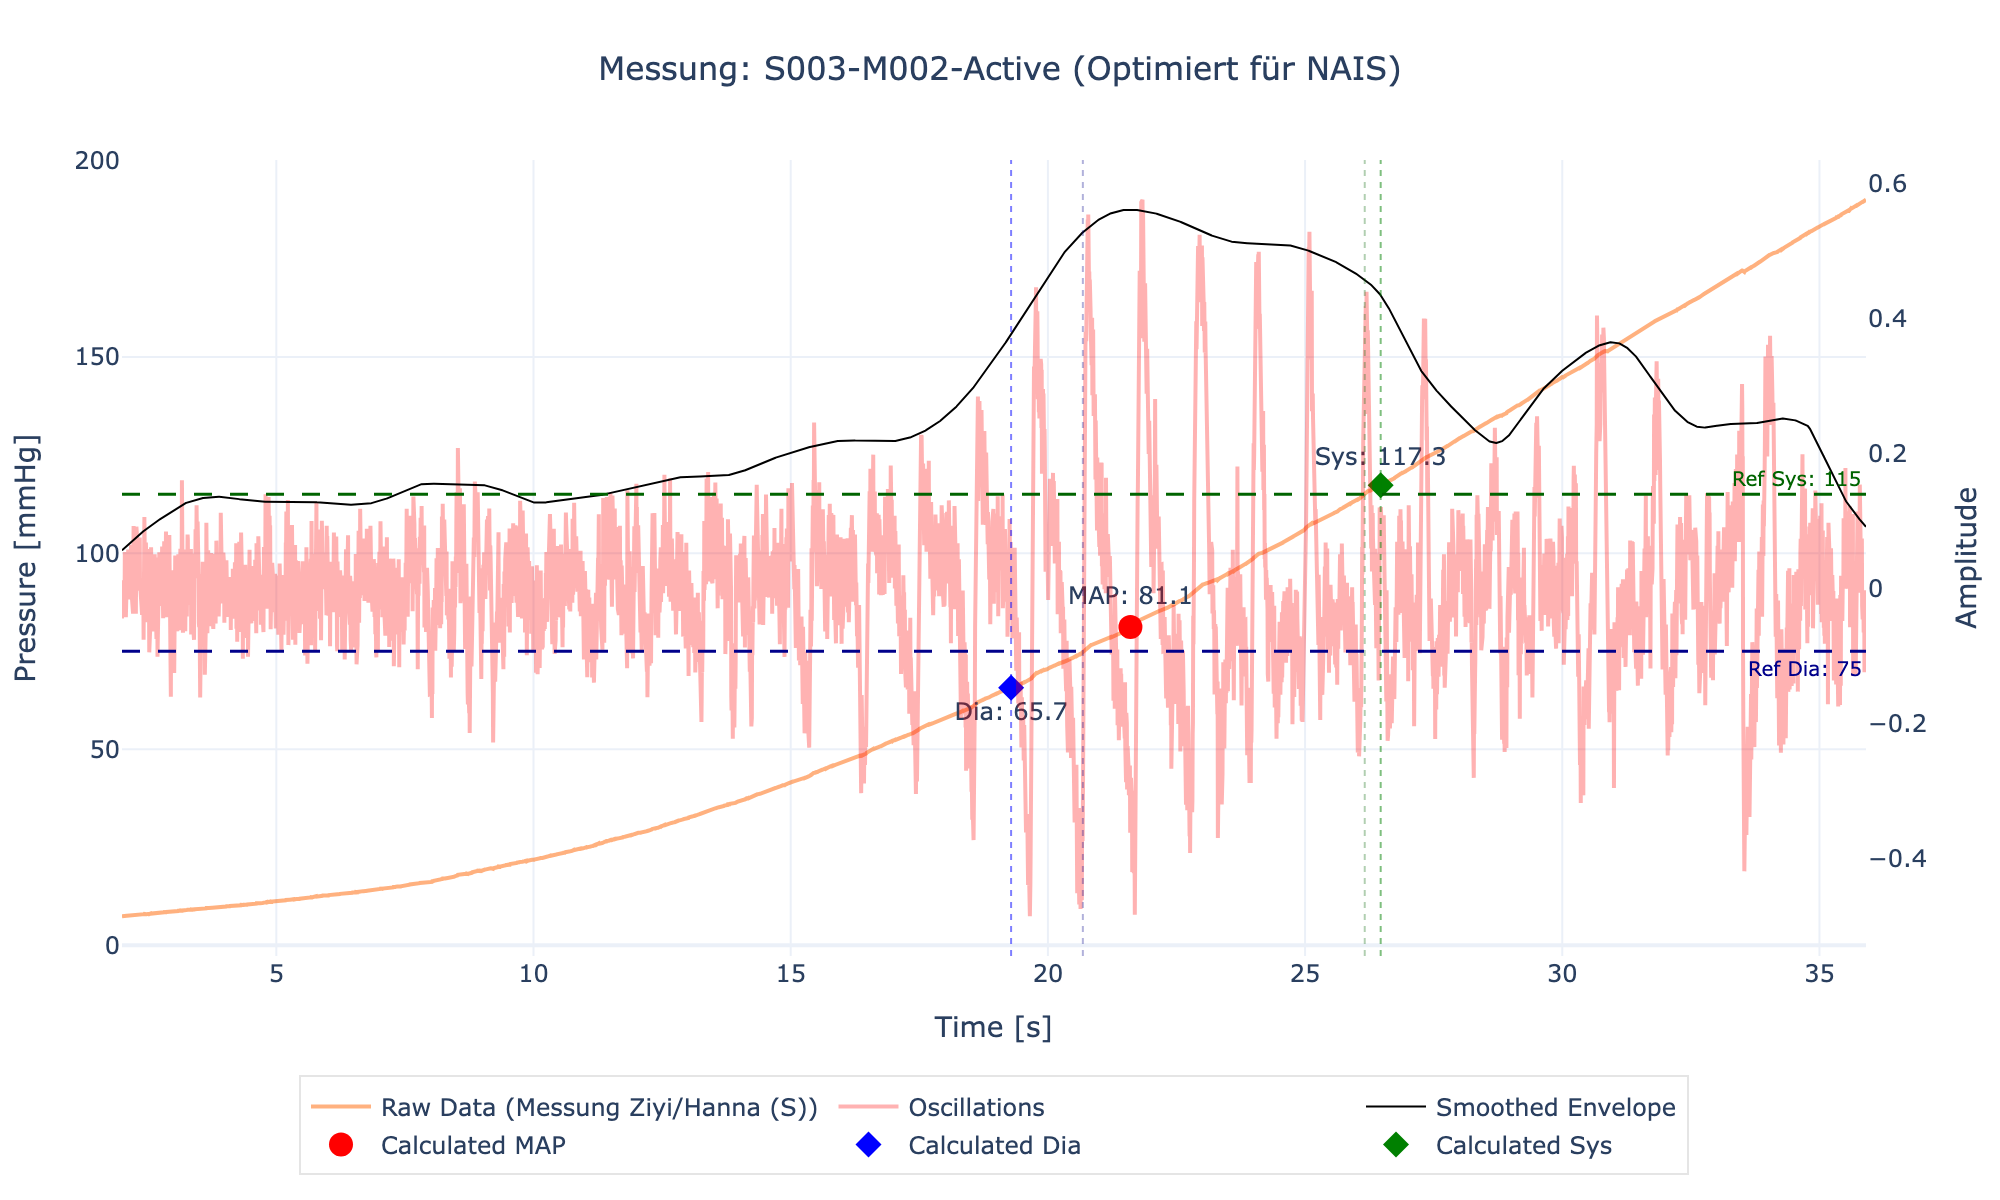
\includegraphics[width=\textwidth]{images/S003-M002-Active_nais.png}
        \caption{Optimiert für NAIS}
    \end{subfigure}
    \caption{Einzelauswertung der Messung S003-M002-Active mit verschiedenen Parametersätzen.}
\end{figure}
\newpage

\subsection*{Messung: S004-M001-Rest}
\begin{figure}[H]
    \centering
    \begin{subfigure}[b]{0.8\textwidth}
        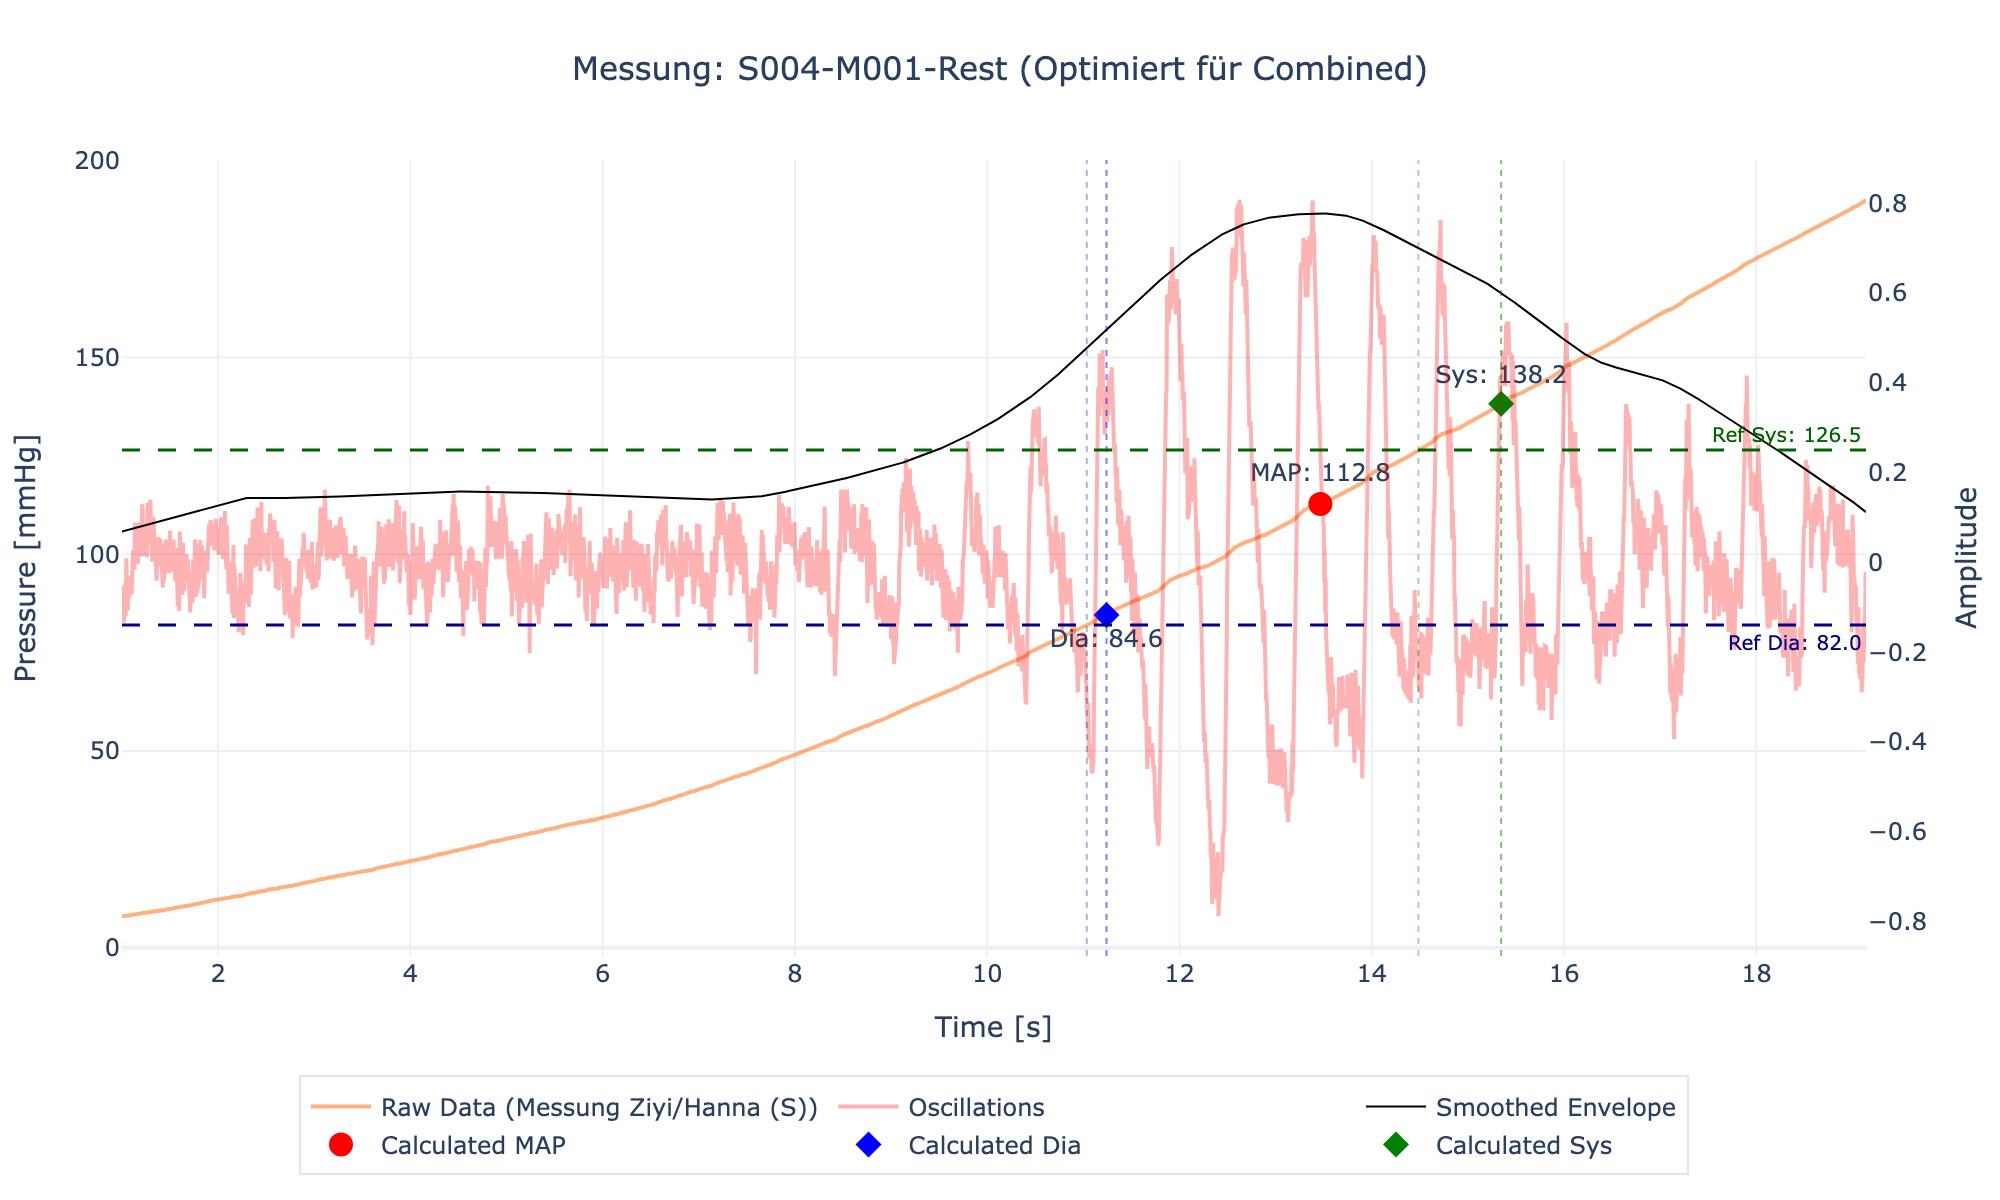
\includegraphics[width=\textwidth]{images/S004-M001-Rest_combined.png}
        \caption{Optimiert für Beurer und NAIS (Kombiniert)}
    \end{subfigure} \\
    \begin{subfigure}[b]{0.48\textwidth}
        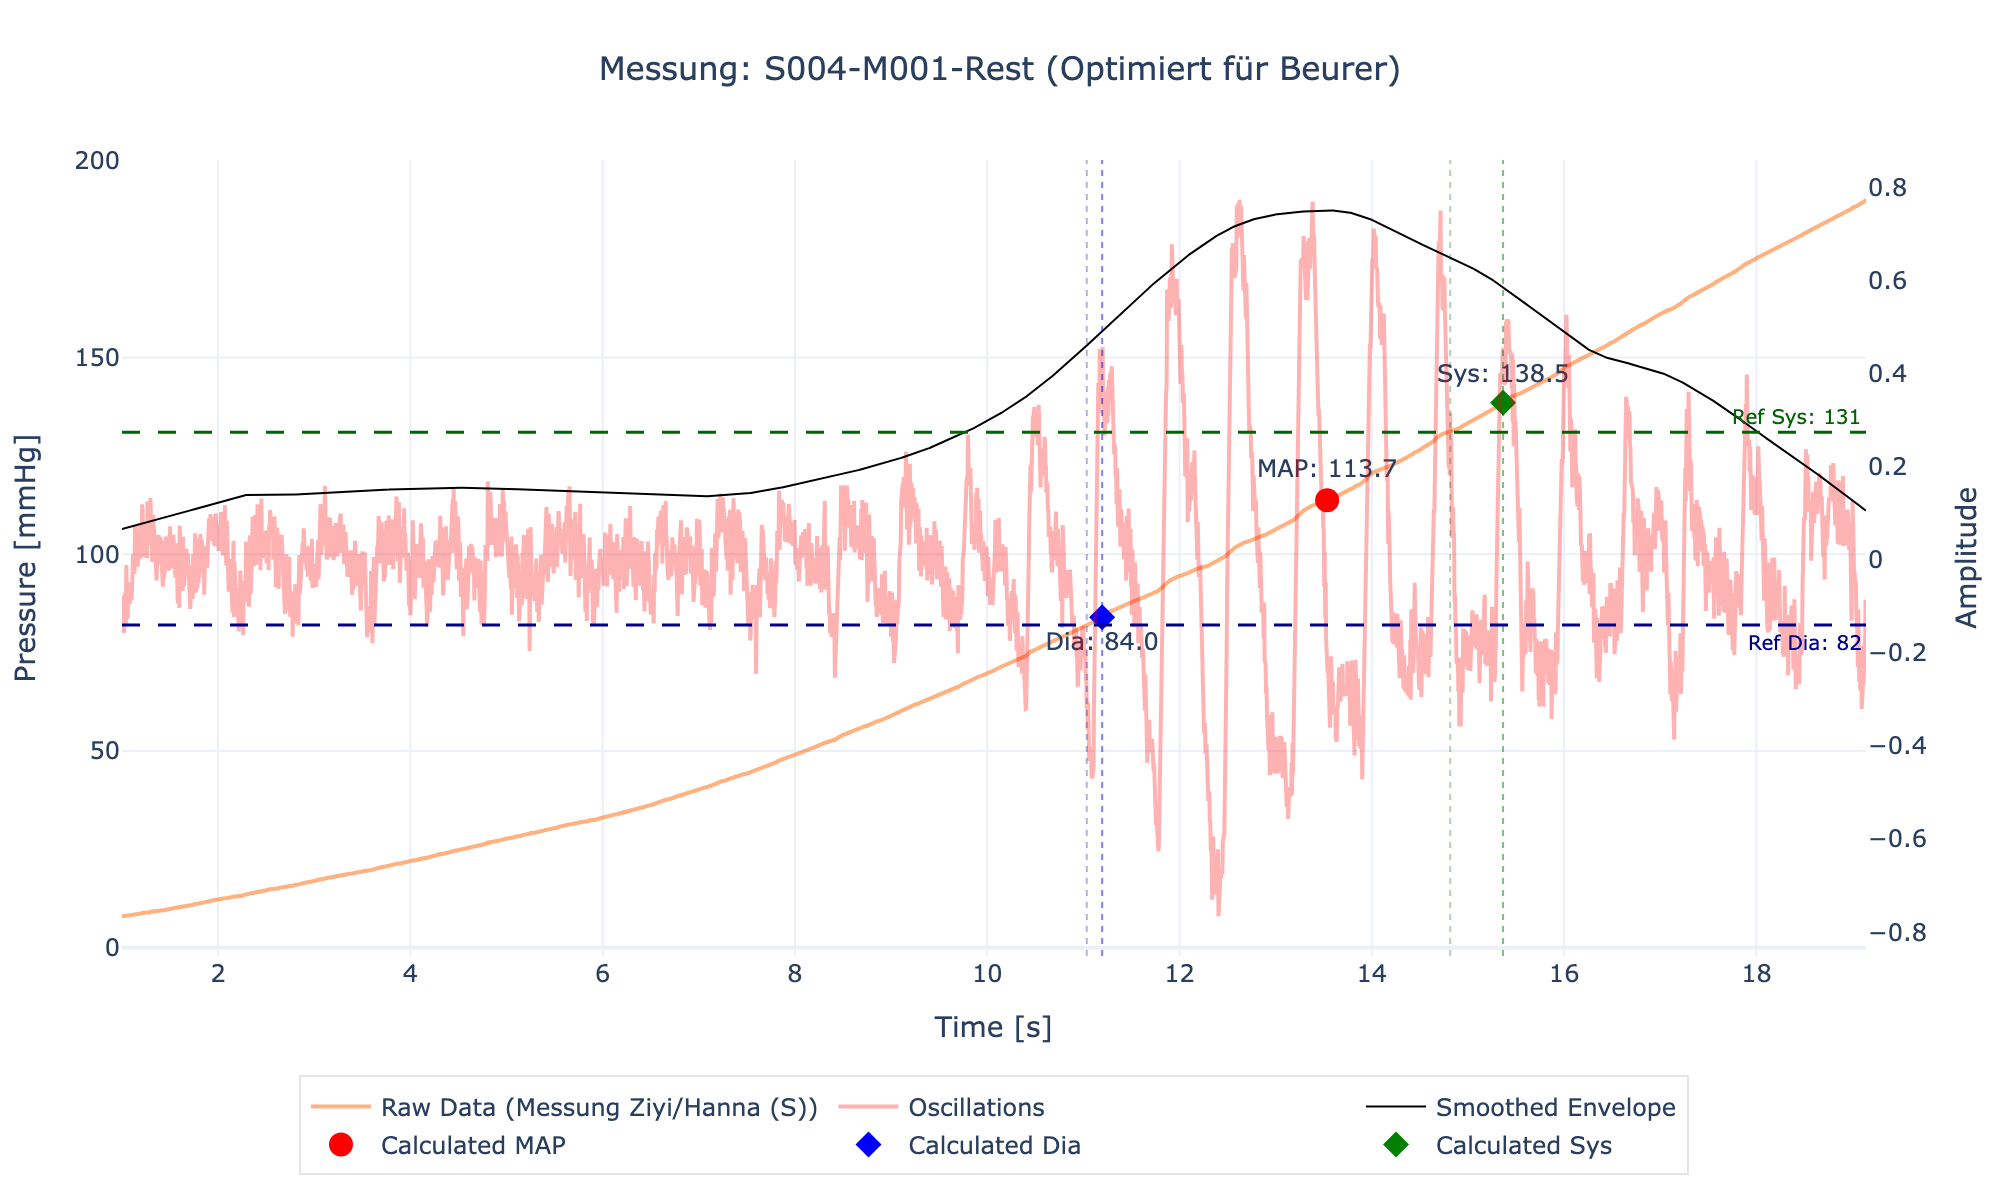
\includegraphics[width=\textwidth]{images/S004-M001-Rest_beurer.png}
        \caption{Optimiert für Beurer}
    \end{subfigure}
    \hfill
    \begin{subfigure}[b]{0.48\textwidth}
        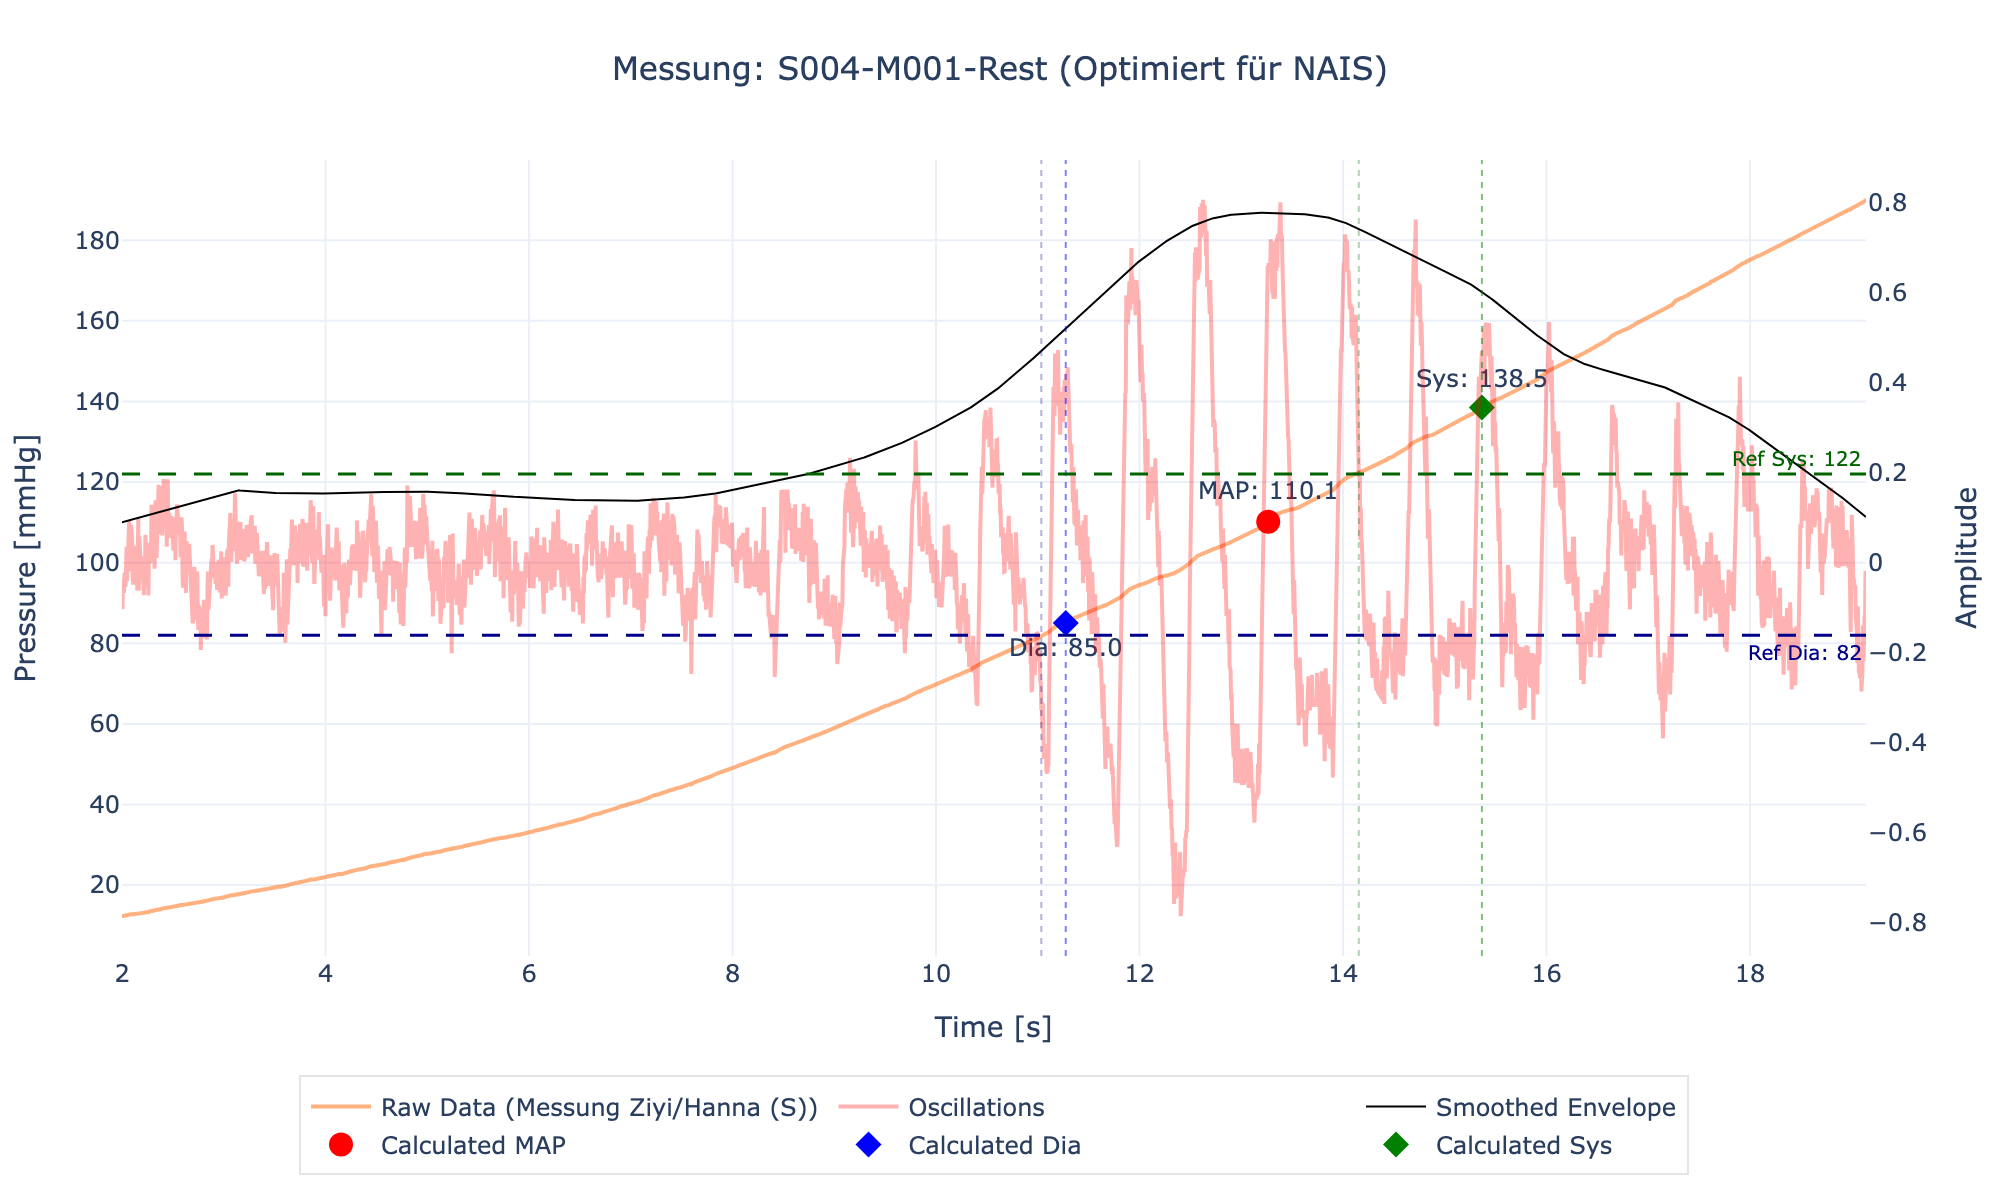
\includegraphics[width=\textwidth]{images/S004-M001-Rest_nais.png}
        \caption{Optimiert für NAIS}
    \end{subfigure}
    \caption{Einzelauswertung der Messung S004-M001-Rest mit verschiedenen Parametersätzen.}
\end{figure}
\newpage

\subsection*{Messung: S004-M002-Active}
\begin{figure}[H]
    \centering
    \begin{subfigure}[b]{0.8\textwidth}
        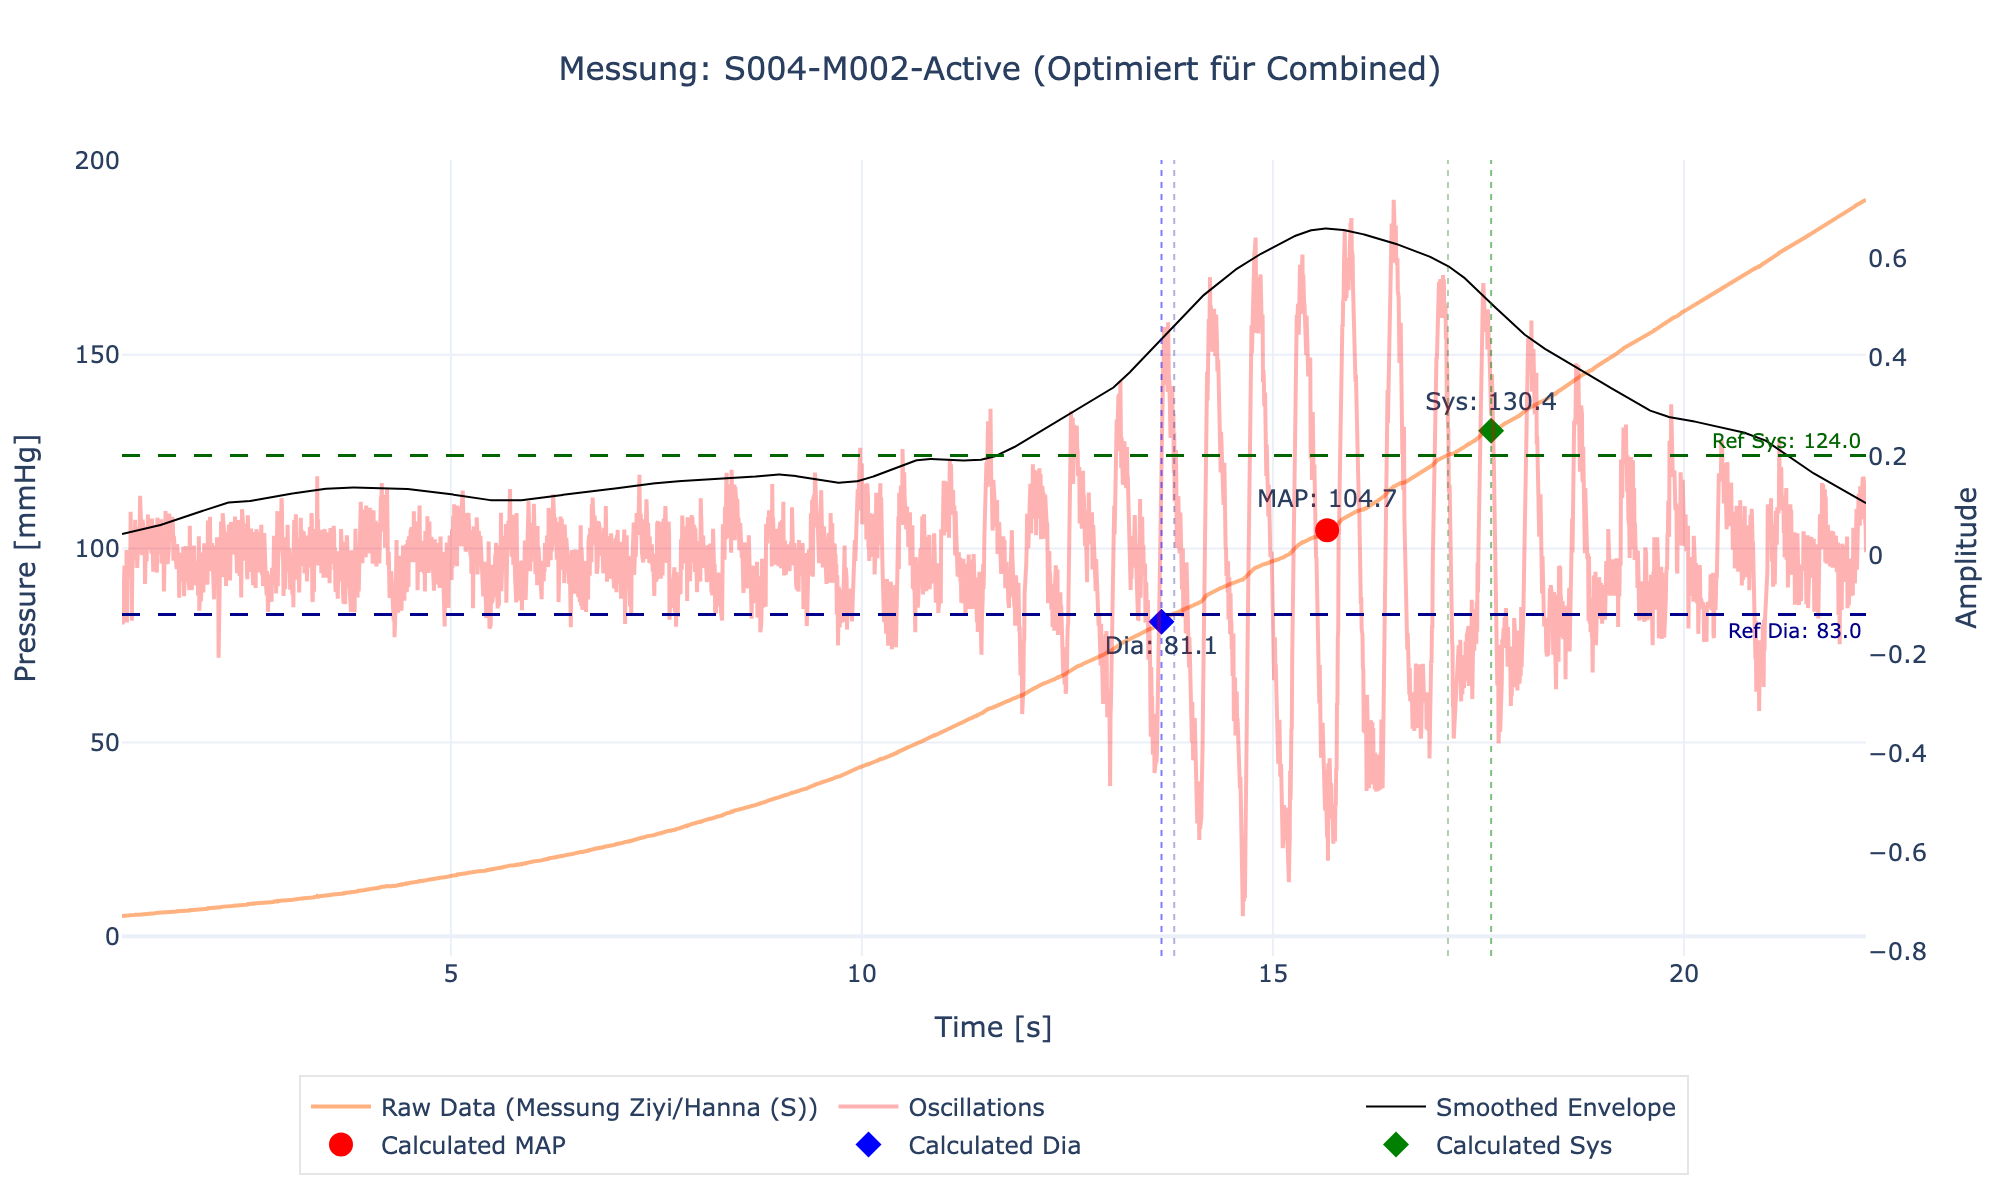
\includegraphics[width=\textwidth]{images/S004-M002-Active_combined.png}
        \caption{Optimiert für Beurer und NAIS (Kombiniert)}
    \end{subfigure} \\
    \begin{subfigure}[b]{0.48\textwidth}
        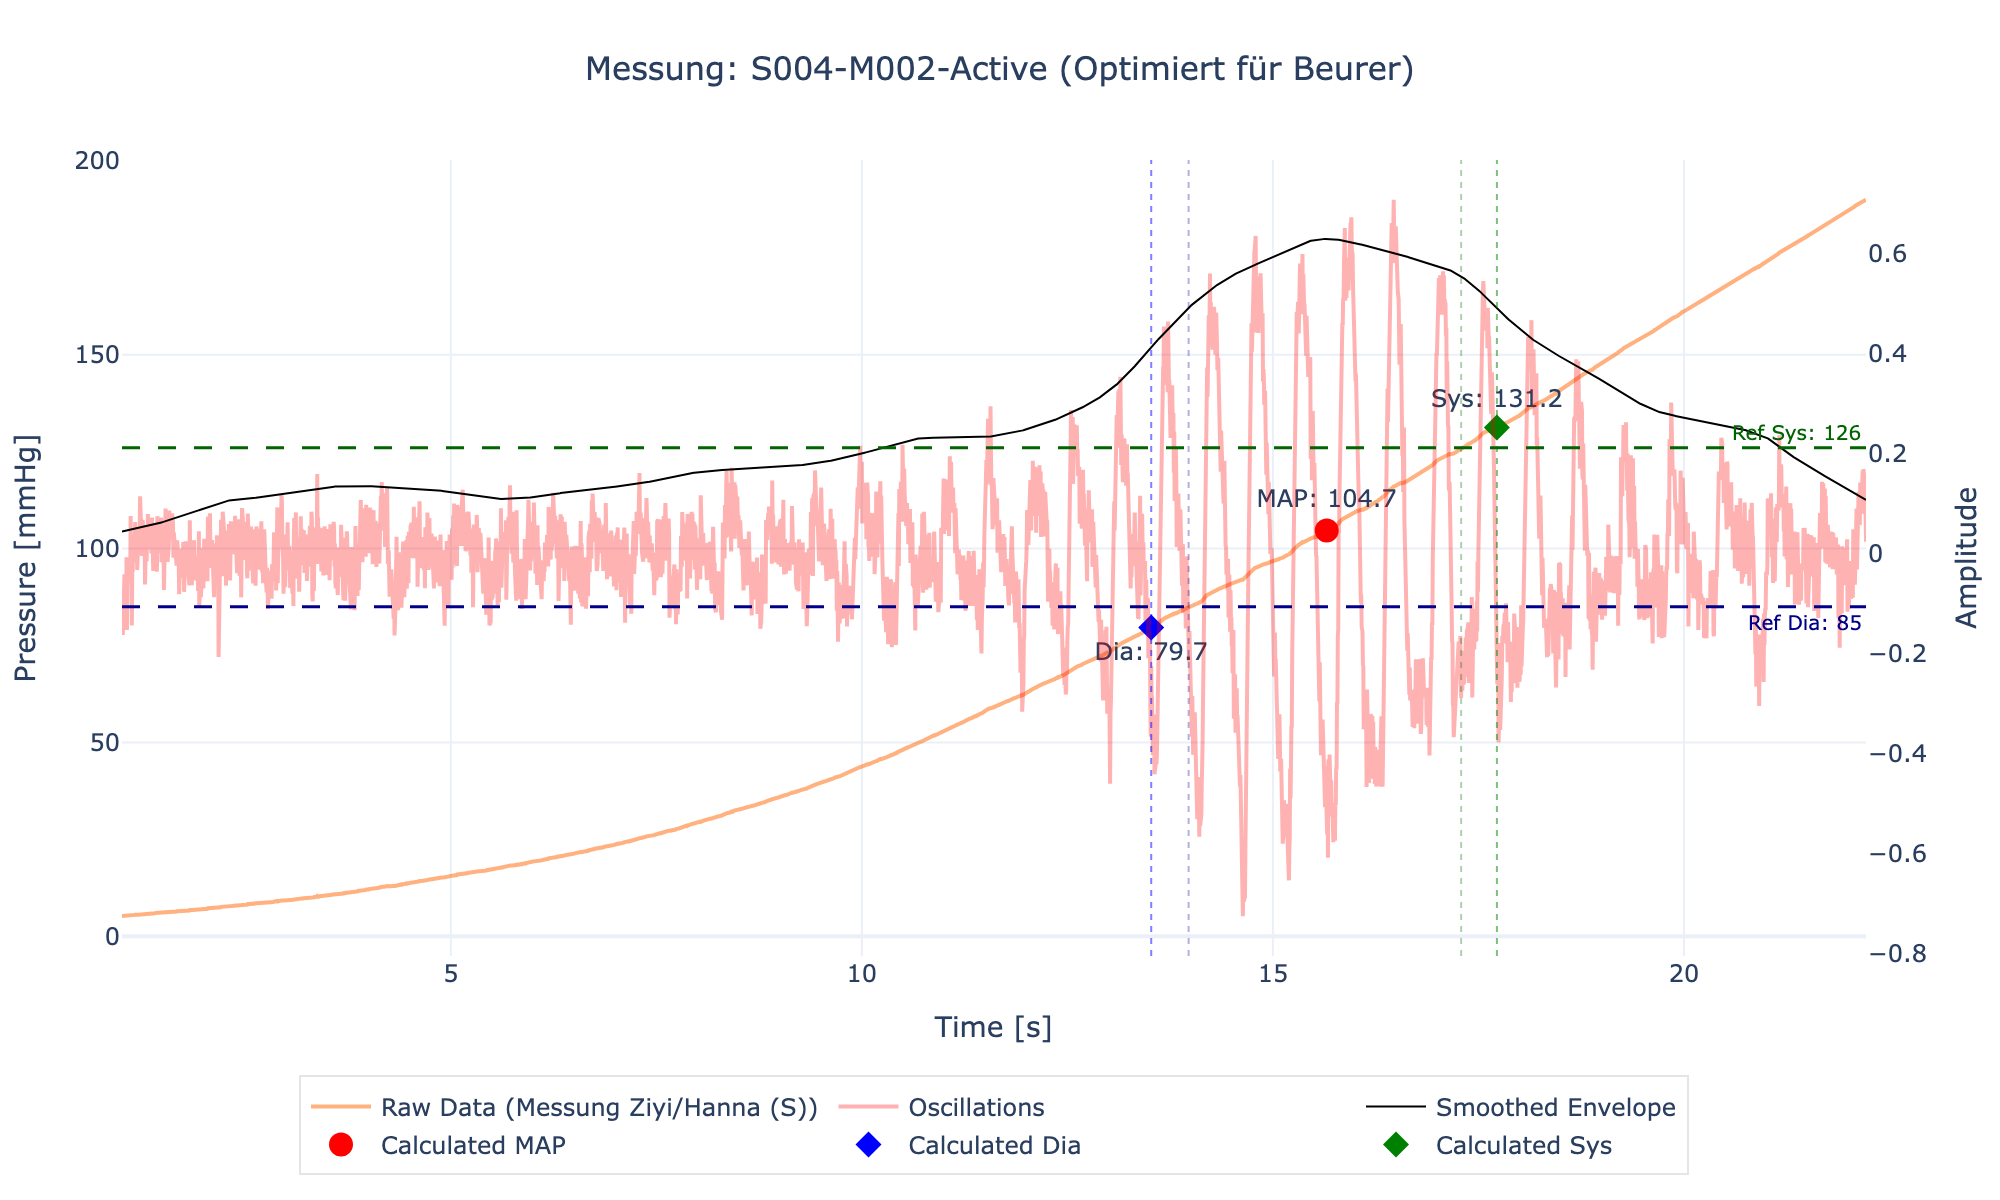
\includegraphics[width=\textwidth]{images/S004-M002-Active_beurer.png}
        \caption{Optimiert für Beurer}
    \end{subfigure}
    \hfill
    \begin{subfigure}[b]{0.48\textwidth}
        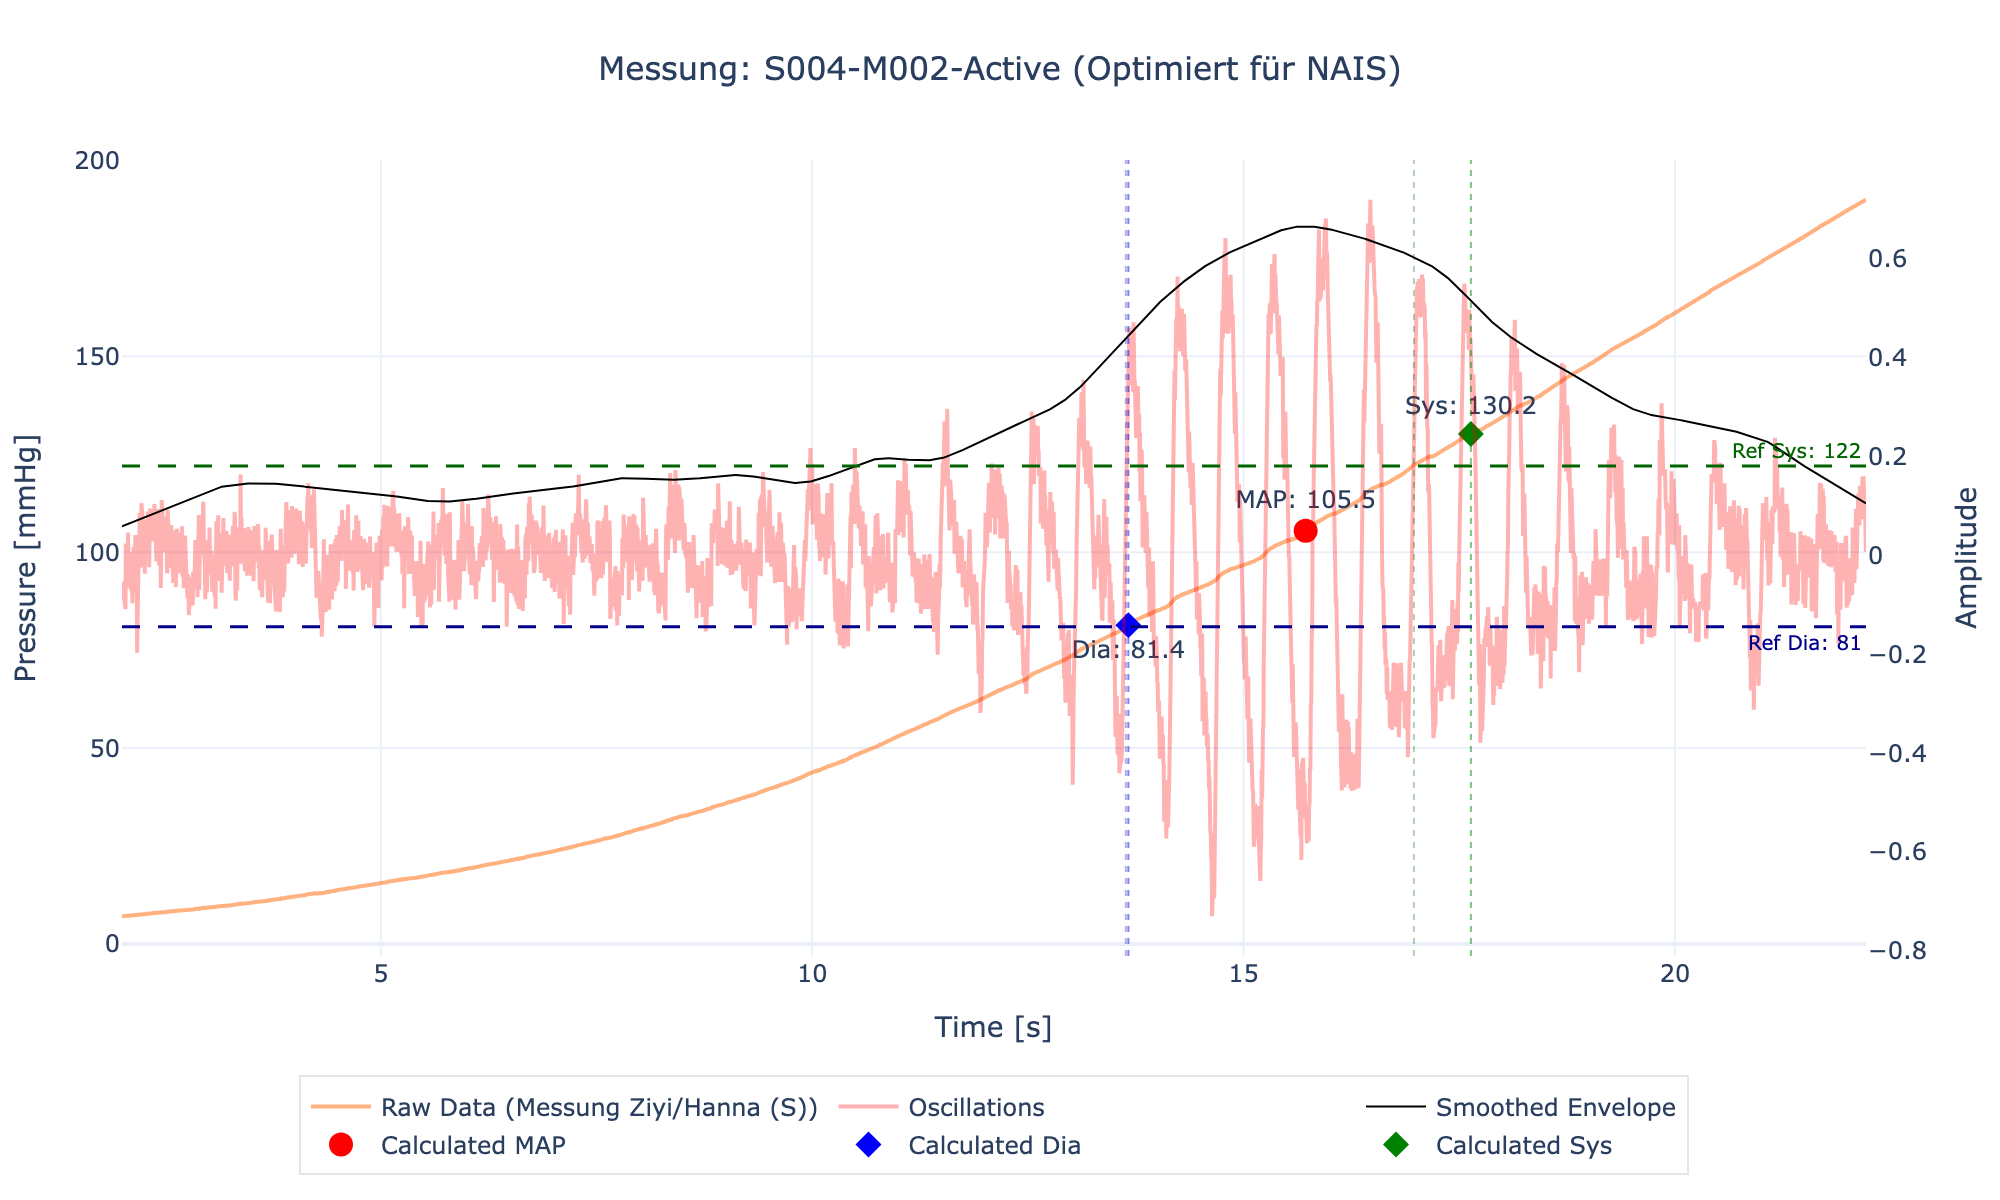
\includegraphics[width=\textwidth]{images/S004-M002-Active_nais.png}
        \caption{Optimiert für NAIS}
    \end{subfigure}
    \caption{Einzelauswertung der Messung S004-M002-Active mit verschiedenen Parametersätzen.}
\end{figure}
\newpage

\subsection*{Messung: S005-M001-Rest}
\begin{figure}[H]
    \centering
    \begin{subfigure}[b]{0.8\textwidth}
        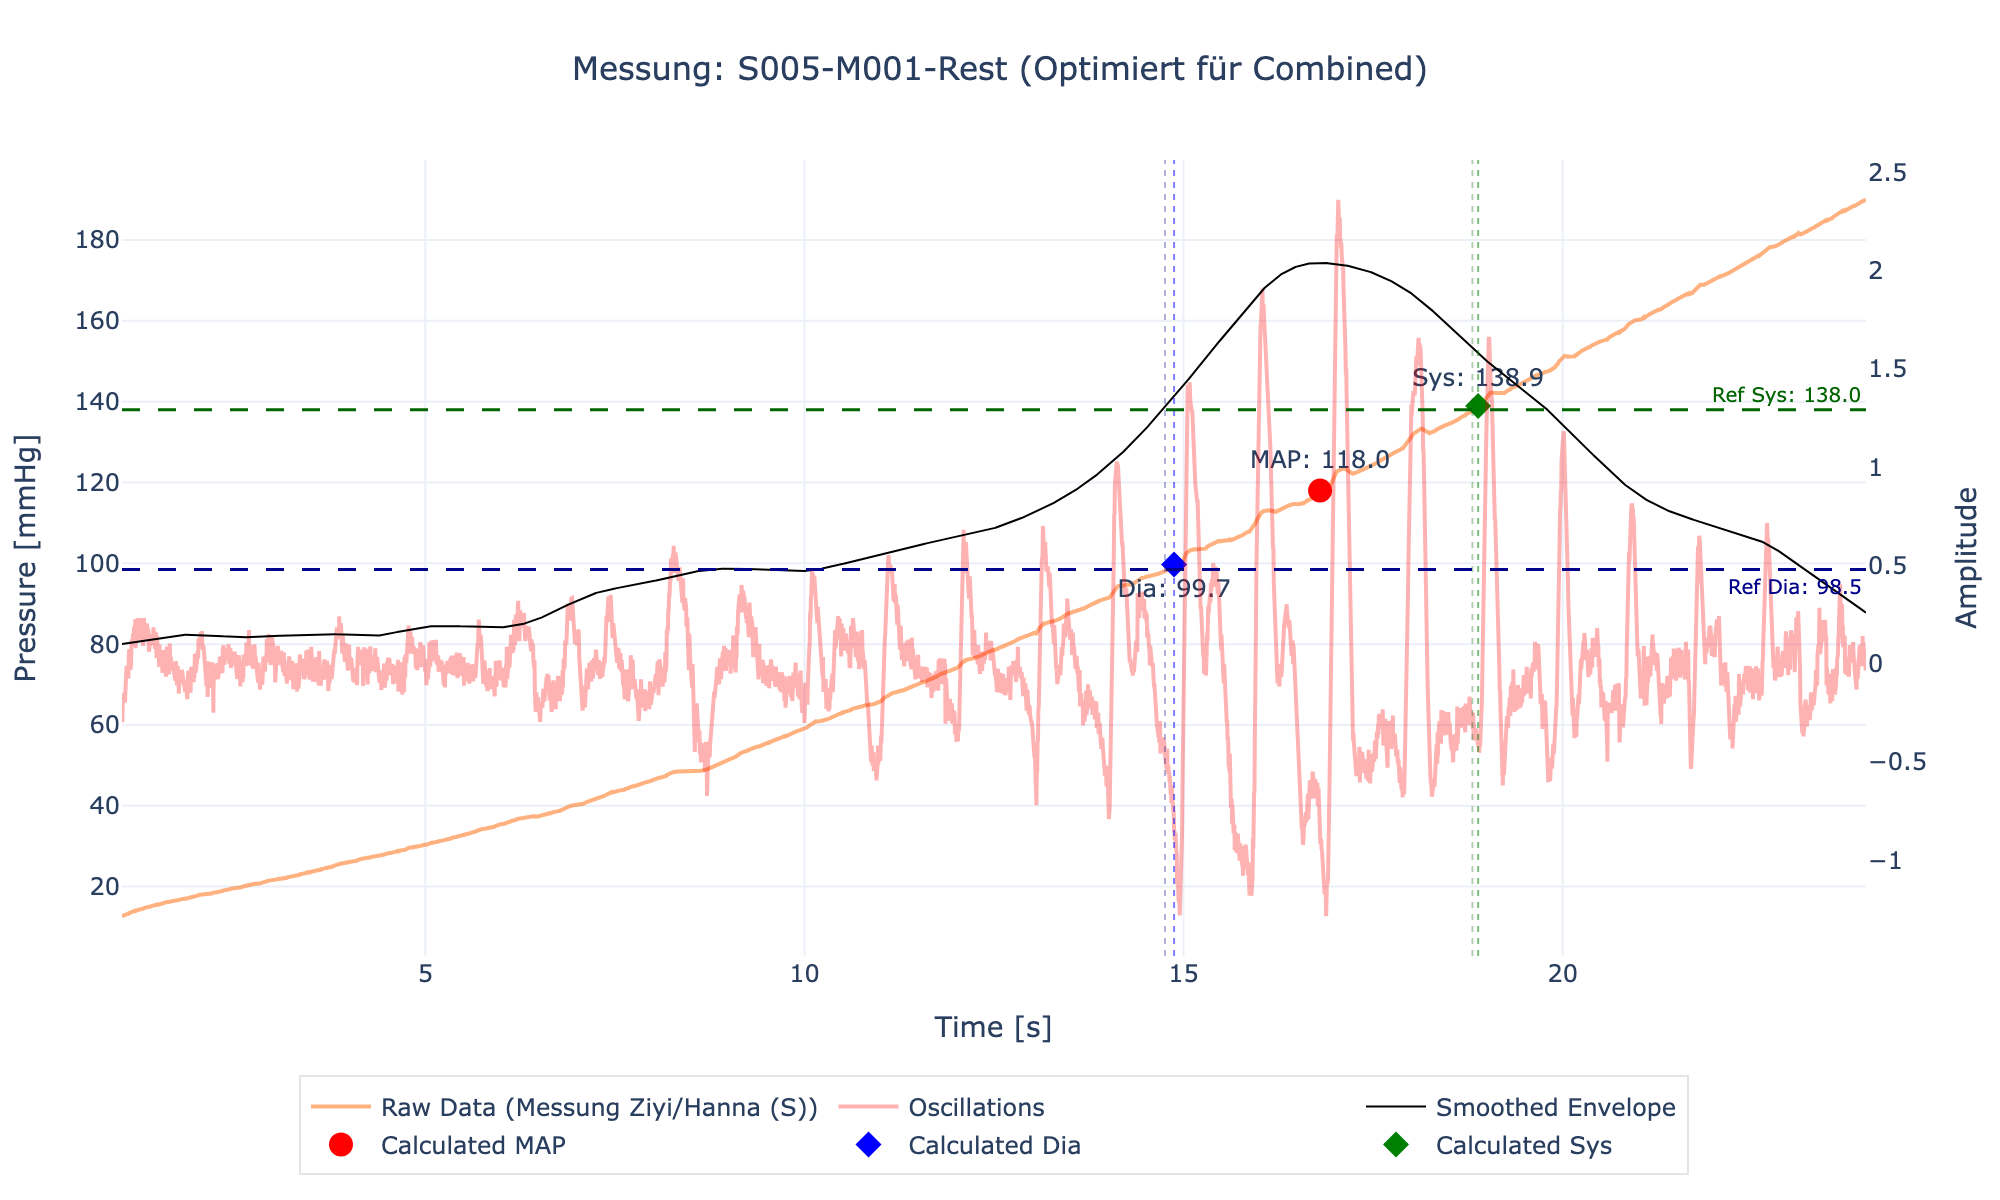
\includegraphics[width=\textwidth]{images/S005-M001-Rest_combined.png}
        \caption{Optimiert für Beurer und NAIS (Kombiniert)}
    \end{subfigure} \\
    \begin{subfigure}[b]{0.48\textwidth}
        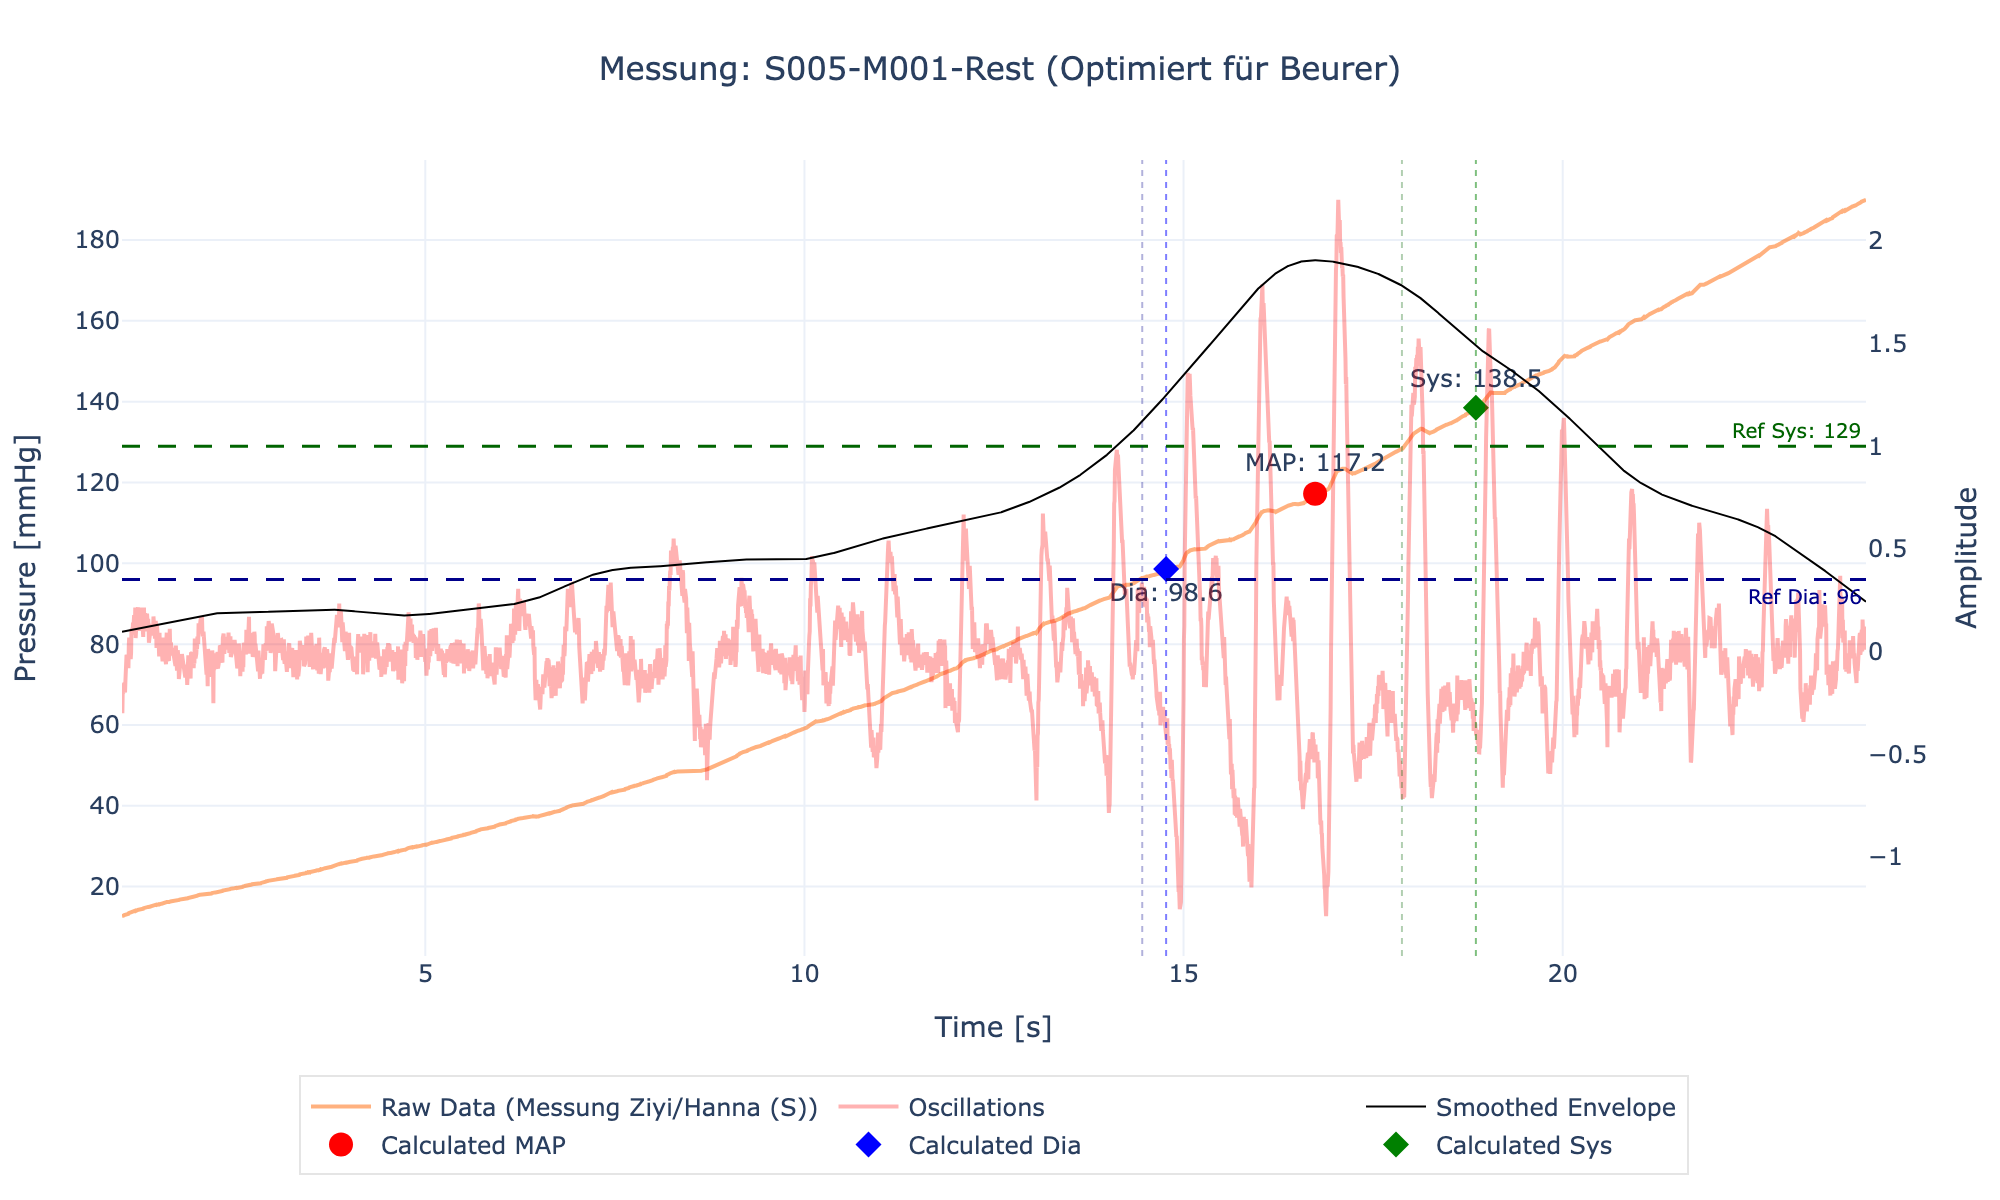
\includegraphics[width=\textwidth]{images/S005-M001-Rest_beurer.png}
        \caption{Optimiert für Beurer}
    \end{subfigure}
    \hfill
    \begin{subfigure}[b]{0.48\textwidth}
        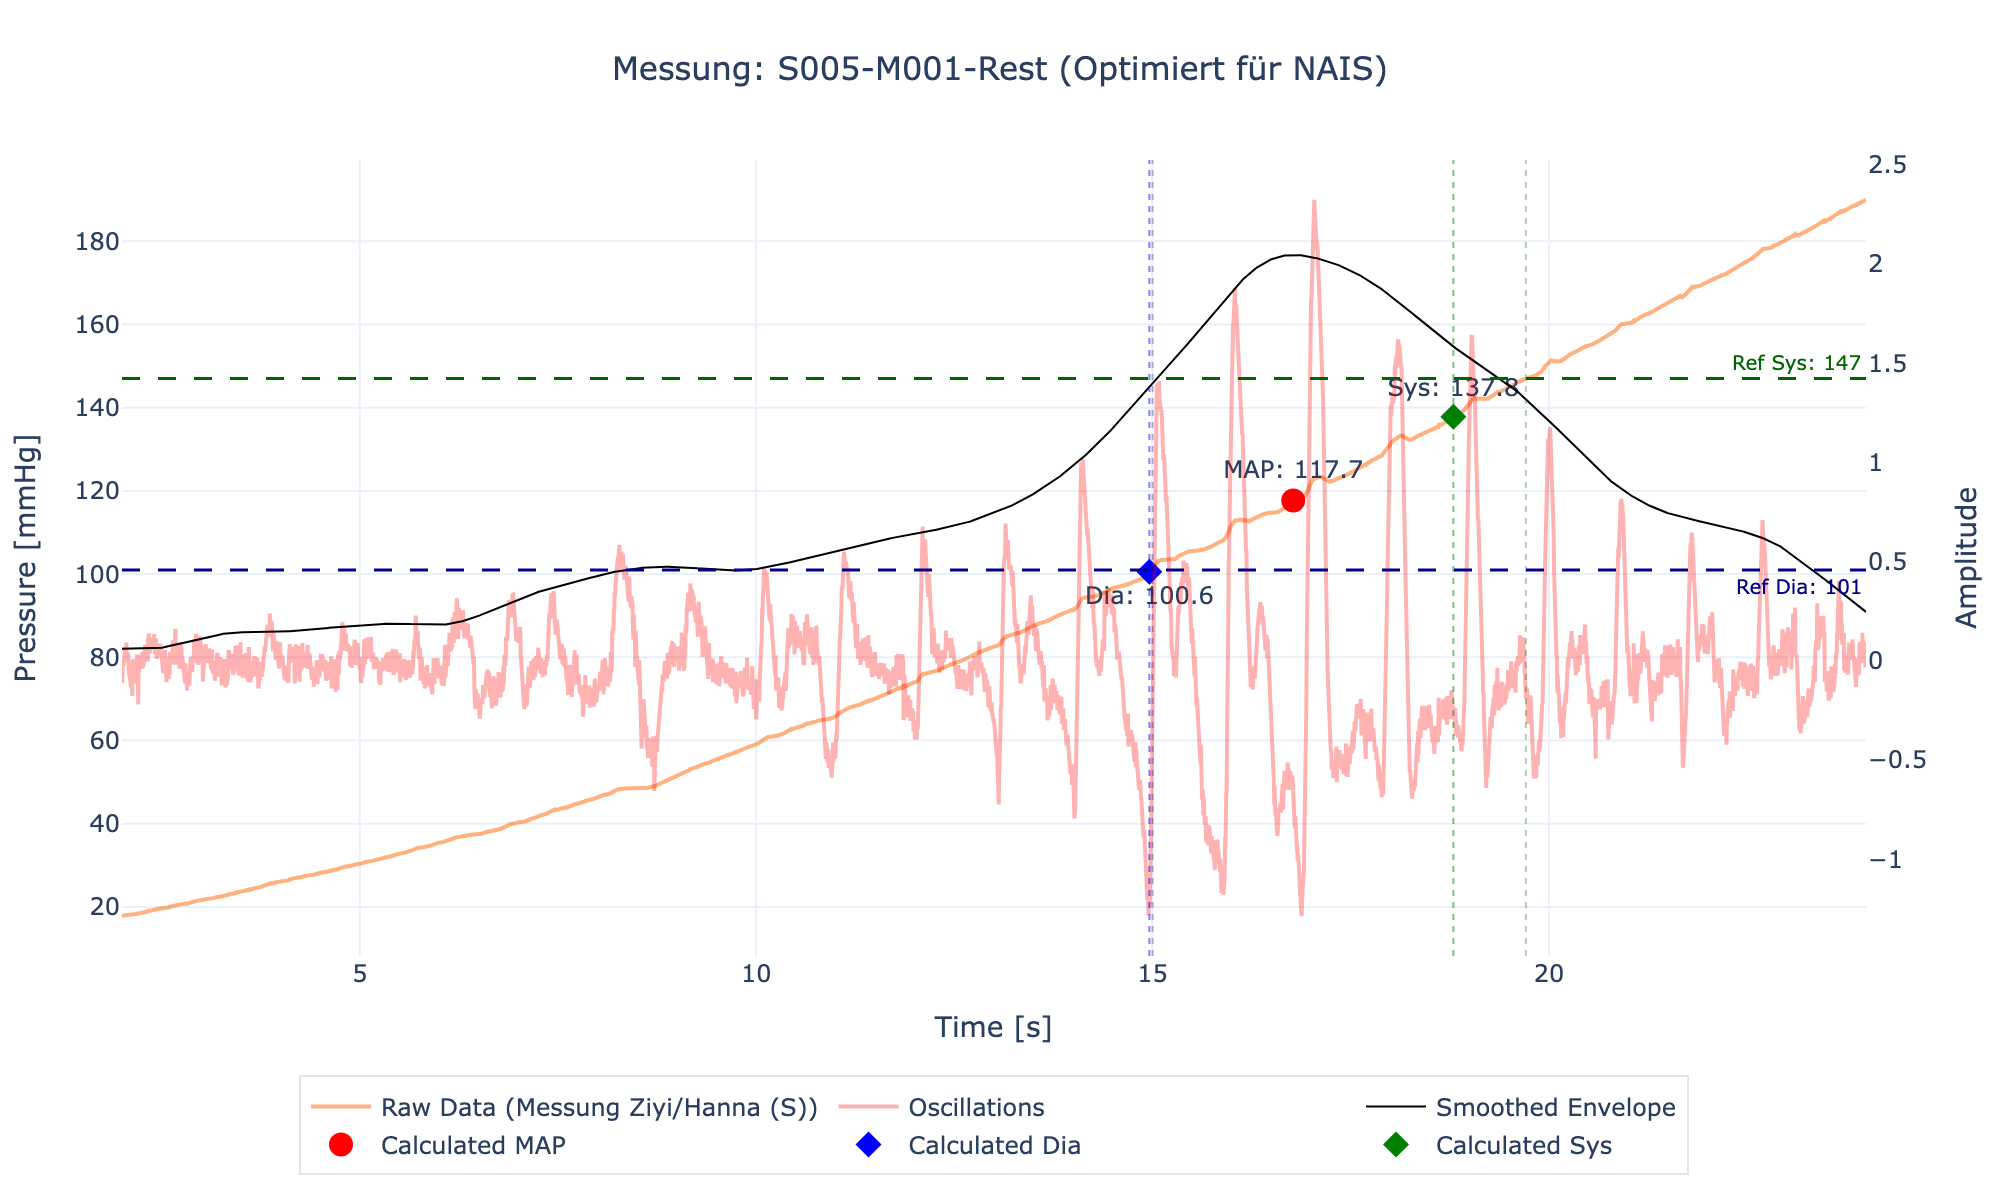
\includegraphics[width=\textwidth]{images/S005-M001-Rest_nais.png}
        \caption{Optimiert für NAIS}
    \end{subfigure}
    \caption{Einzelauswertung der Messung S005-M001-Rest mit verschiedenen Parametersätzen.}
\end{figure}
\newpage

\subsection*{Messung: S005-M002-Active}
\begin{figure}[H]
    \centering
    \begin{subfigure}[b]{0.8\textwidth}
        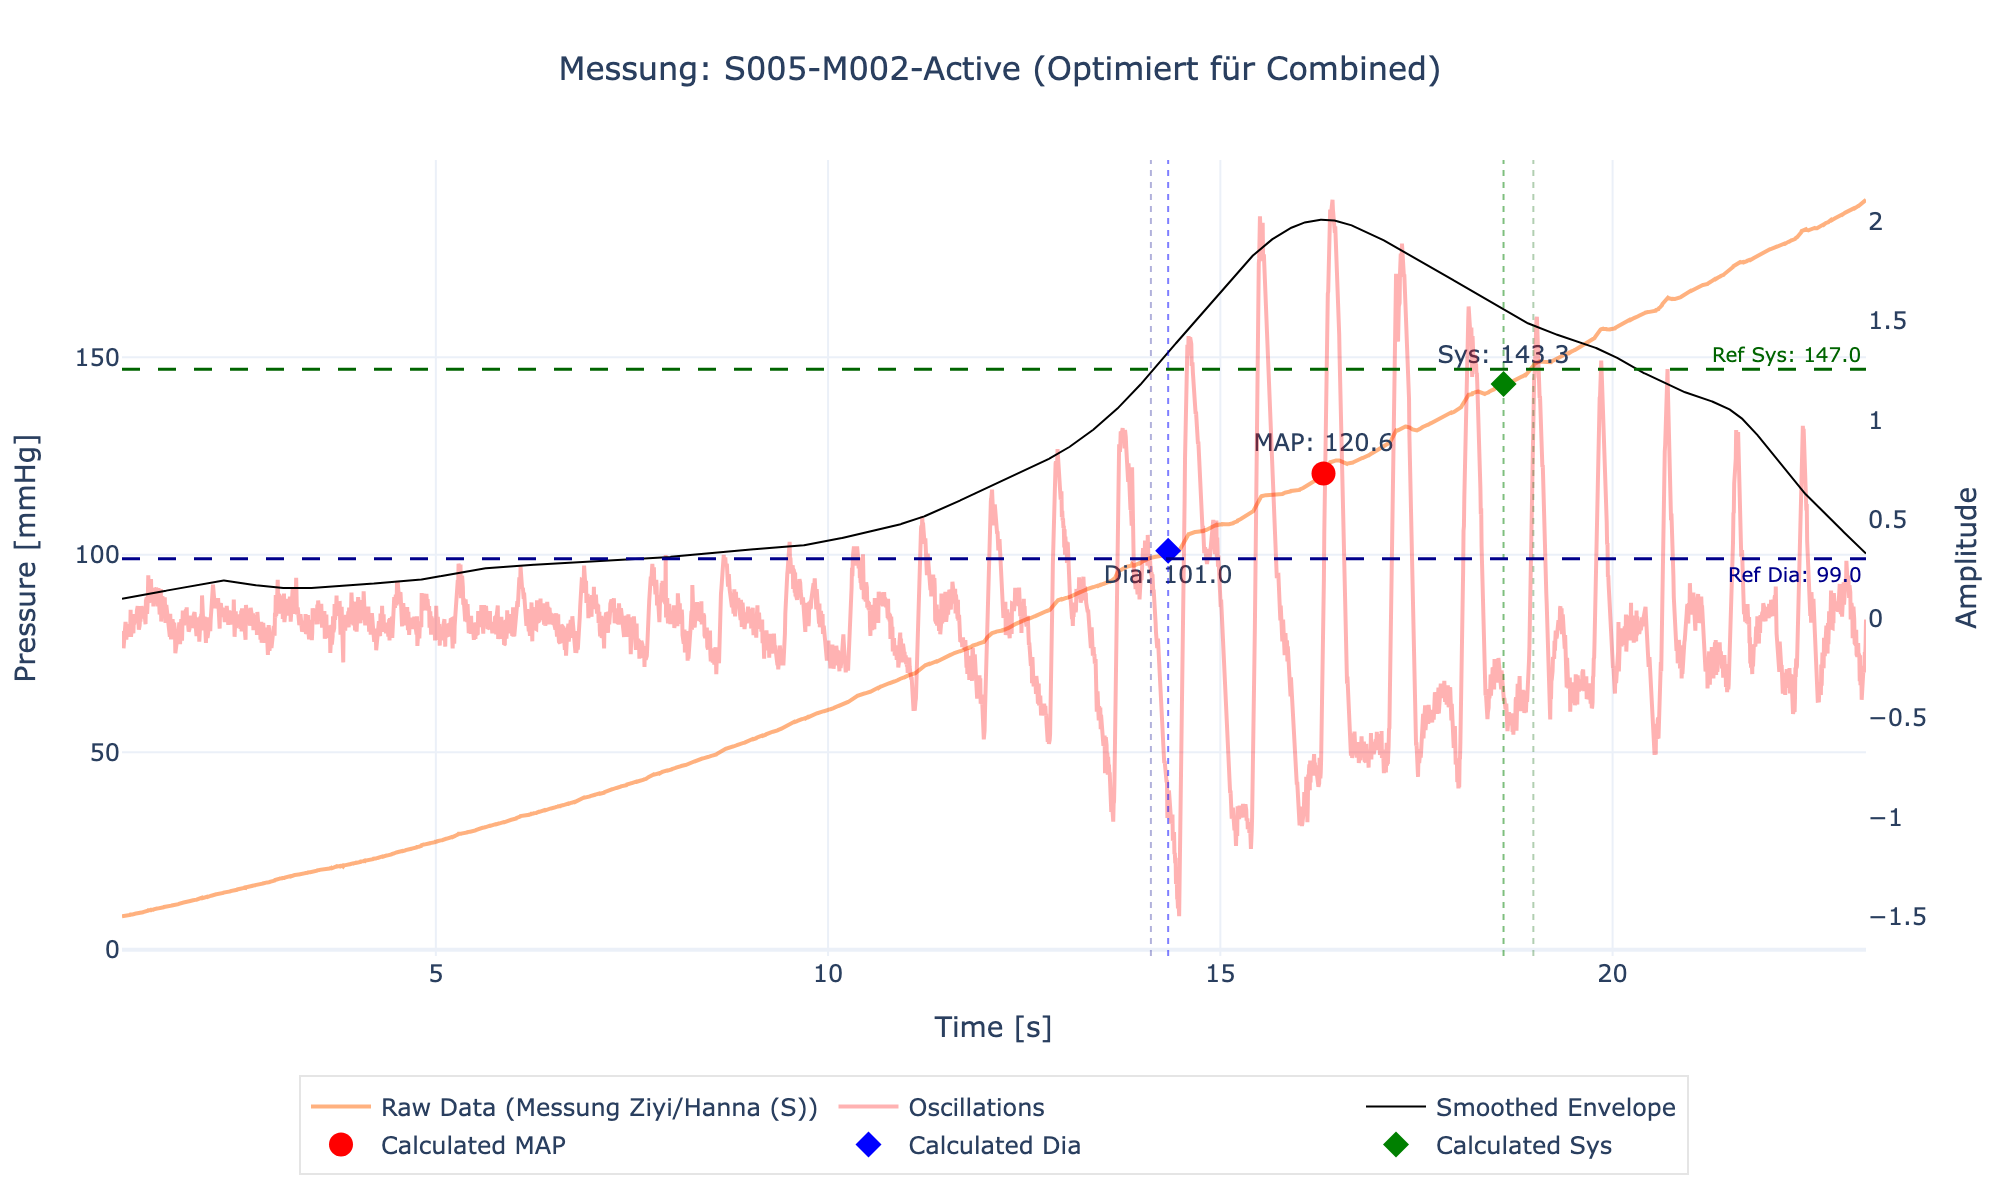
\includegraphics[width=\textwidth]{images/S005-M002-Active_combined.png}
        \caption{Optimiert für Beurer und NAIS (Kombiniert)}
    \end{subfigure} \\
    \begin{subfigure}[b]{0.48\textwidth}
        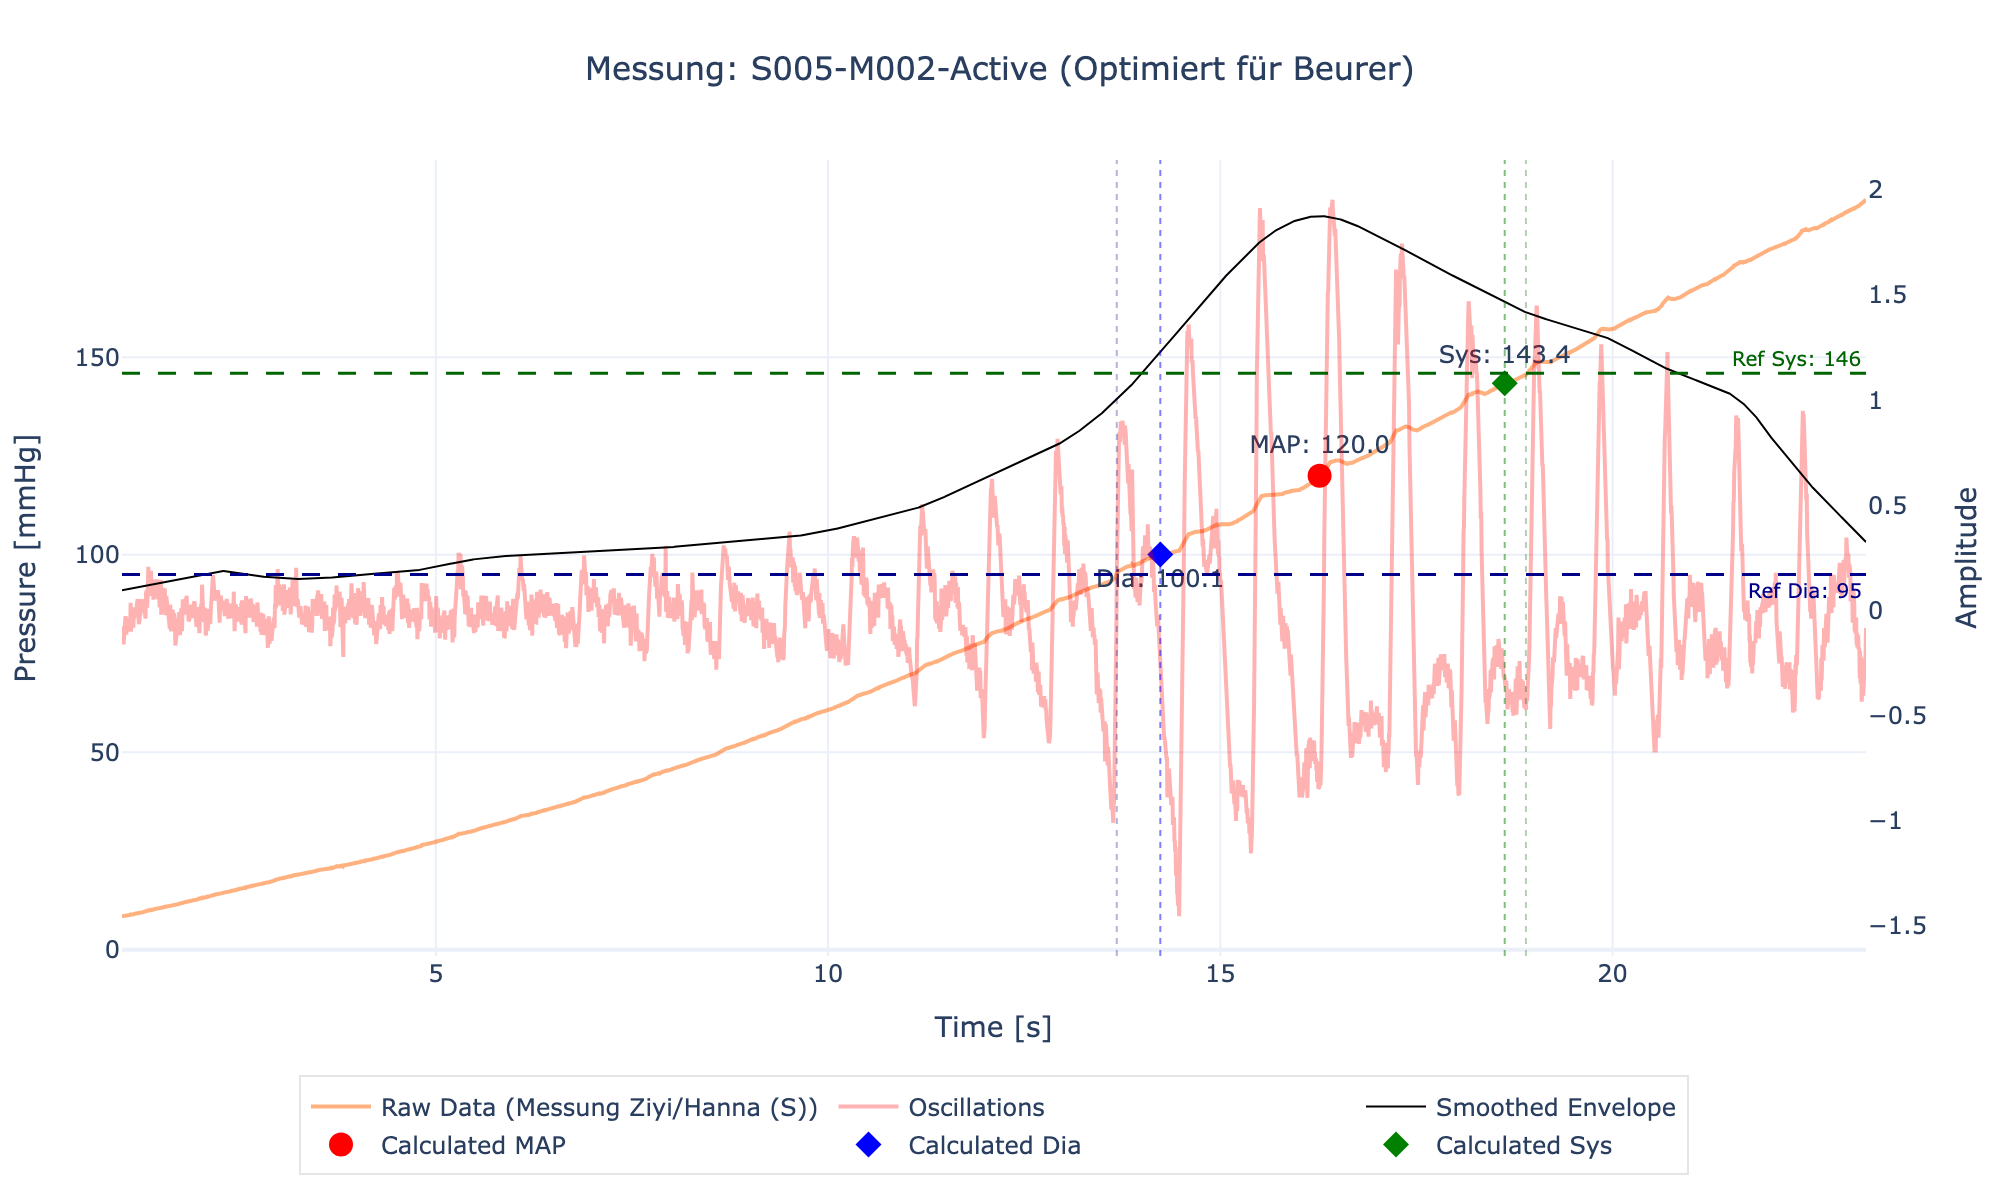
\includegraphics[width=\textwidth]{images/S005-M002-Active_beurer.png}
        \caption{Optimiert für Beurer}
    \end{subfigure}
    \hfill
    \begin{subfigure}[b]{0.48\textwidth}
        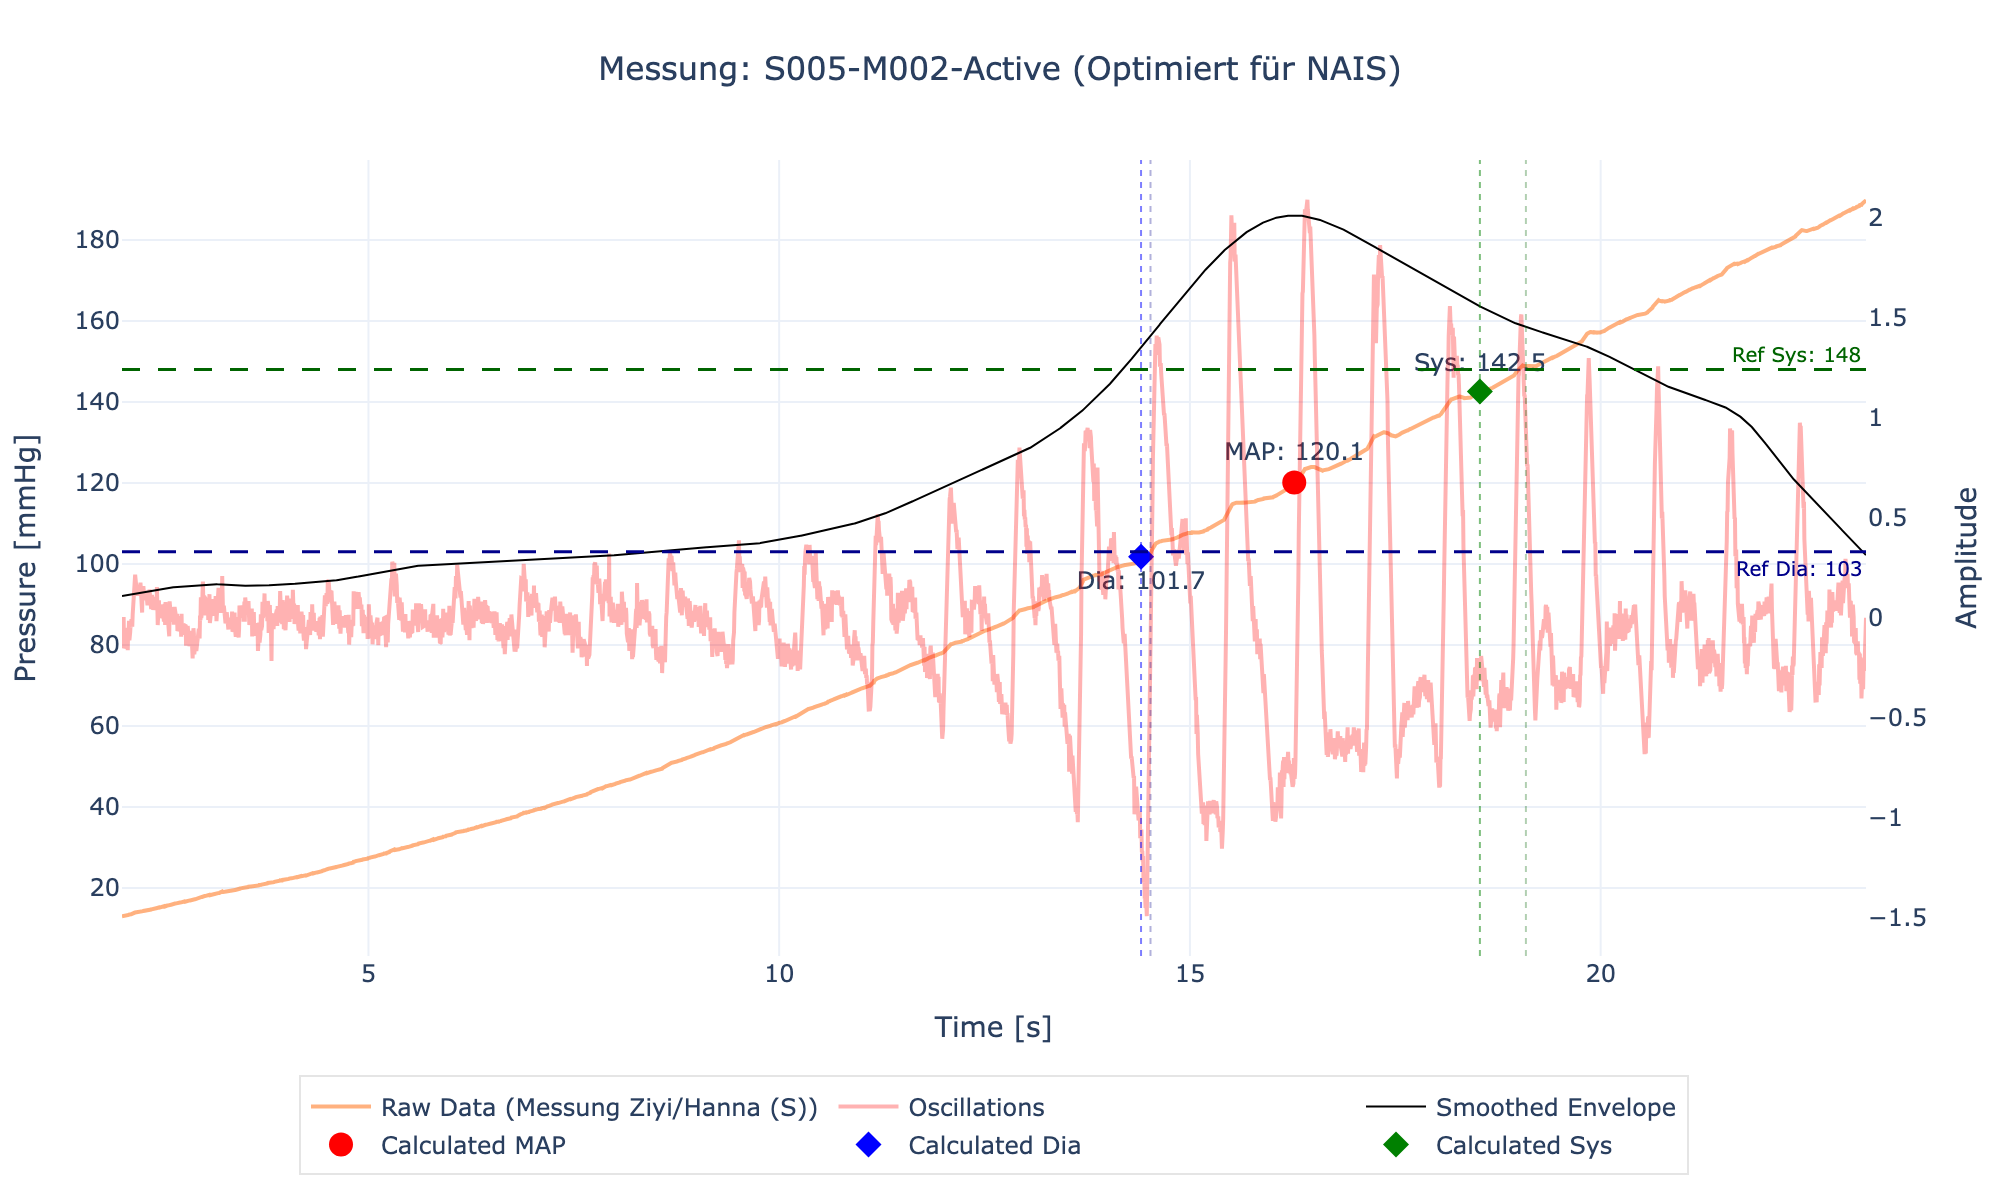
\includegraphics[width=\textwidth]{images/S005-M002-Active_nais.png}
        \caption{Optimiert für NAIS}
    \end{subfigure}
    \caption{Einzelauswertung der Messung S005-M002-Active mit verschiedenen Parametersätzen.}
\end{figure}
\newpage

\subsection*{Messung: S006-M001-Rest}
\begin{figure}[H]
    \centering
    \begin{subfigure}[b]{0.8\textwidth}
        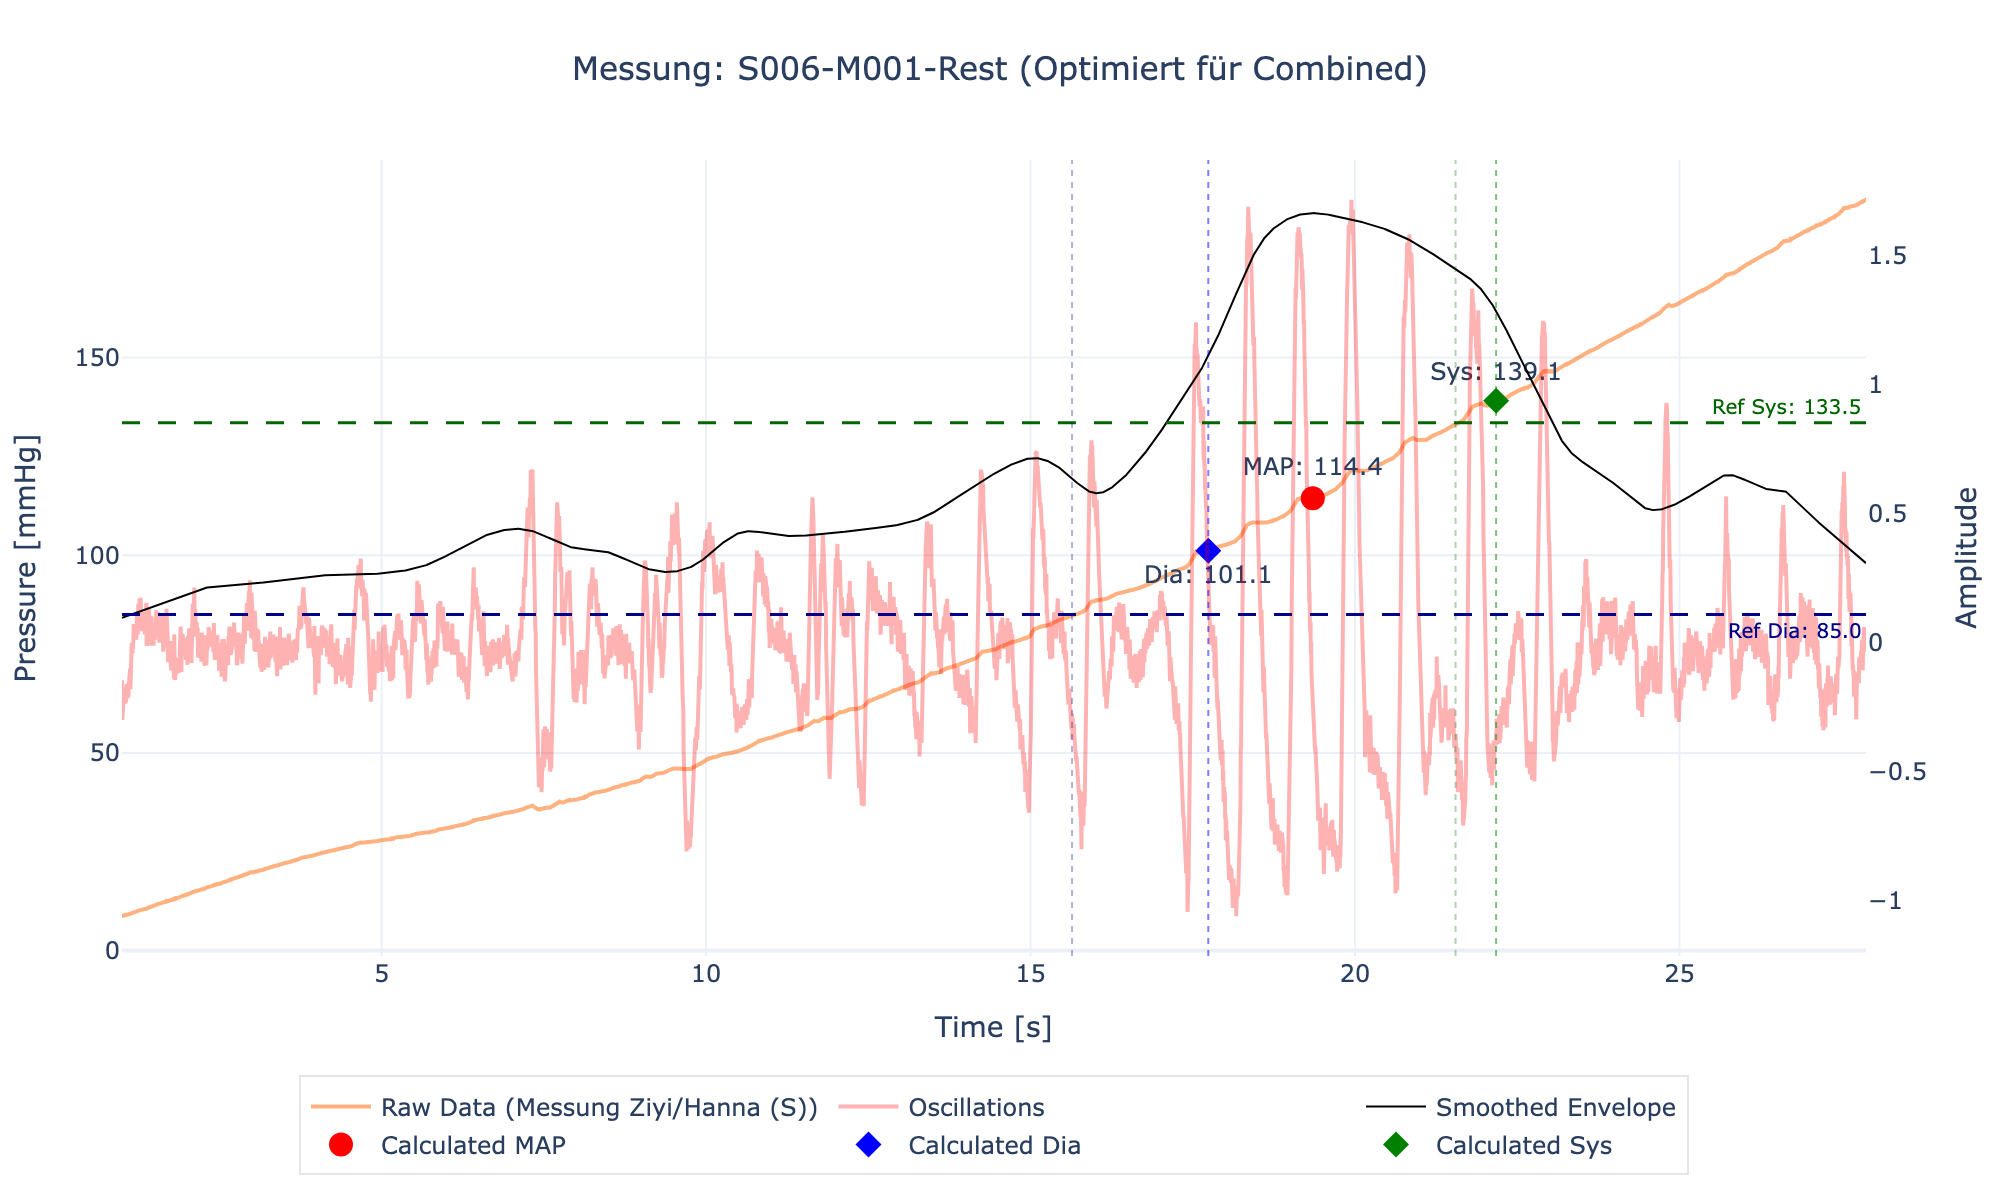
\includegraphics[width=\textwidth]{images/S006-M001-Rest_combined.png}
        \caption{Optimiert für Beurer und NAIS (Kombiniert)}
    \end{subfigure} \\
    \begin{subfigure}[b]{0.48\textwidth}
        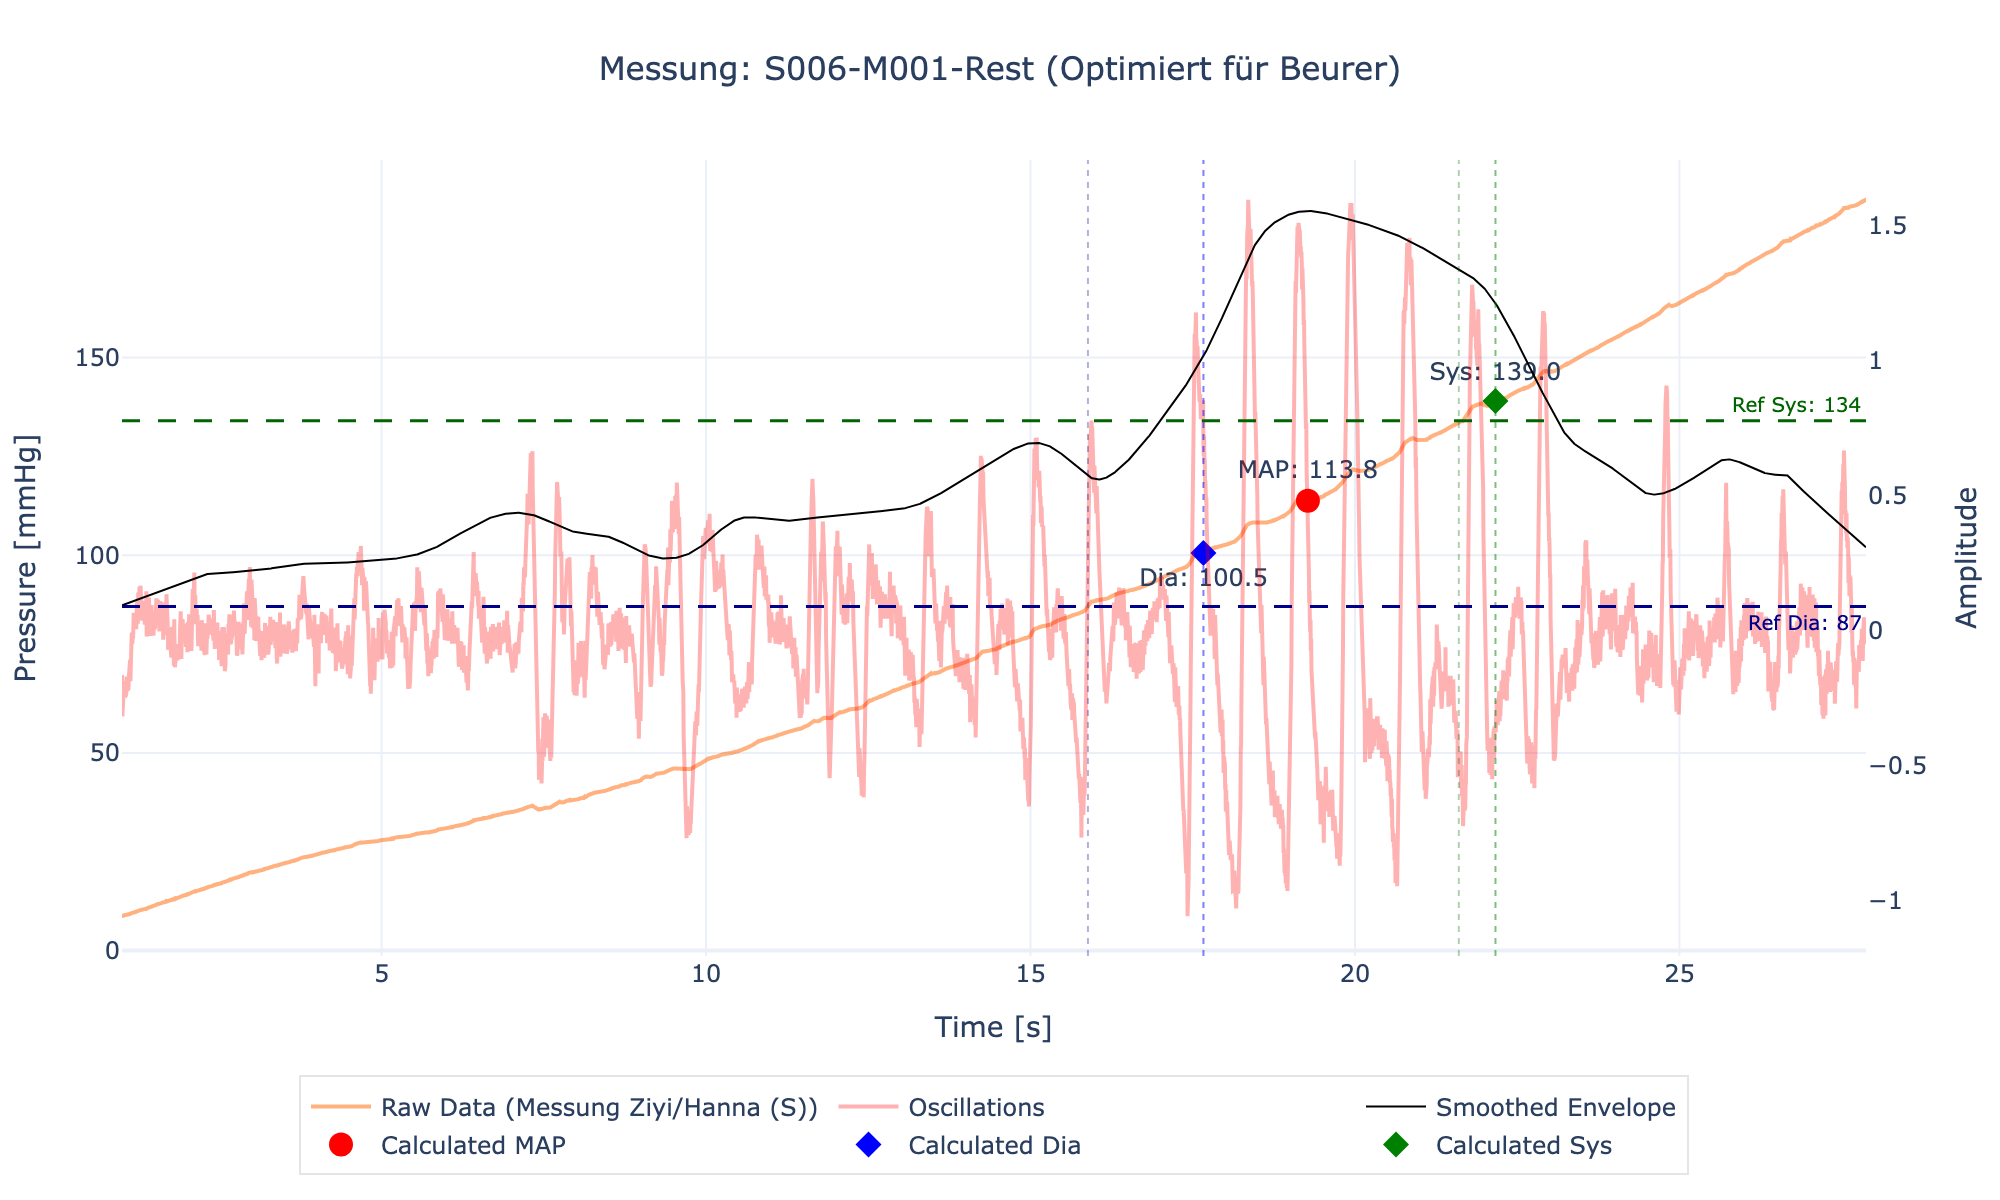
\includegraphics[width=\textwidth]{images/S006-M001-Rest_beurer.png}
        \caption{Optimiert für Beurer}
    \end{subfigure}
    \hfill
    \begin{subfigure}[b]{0.48\textwidth}
        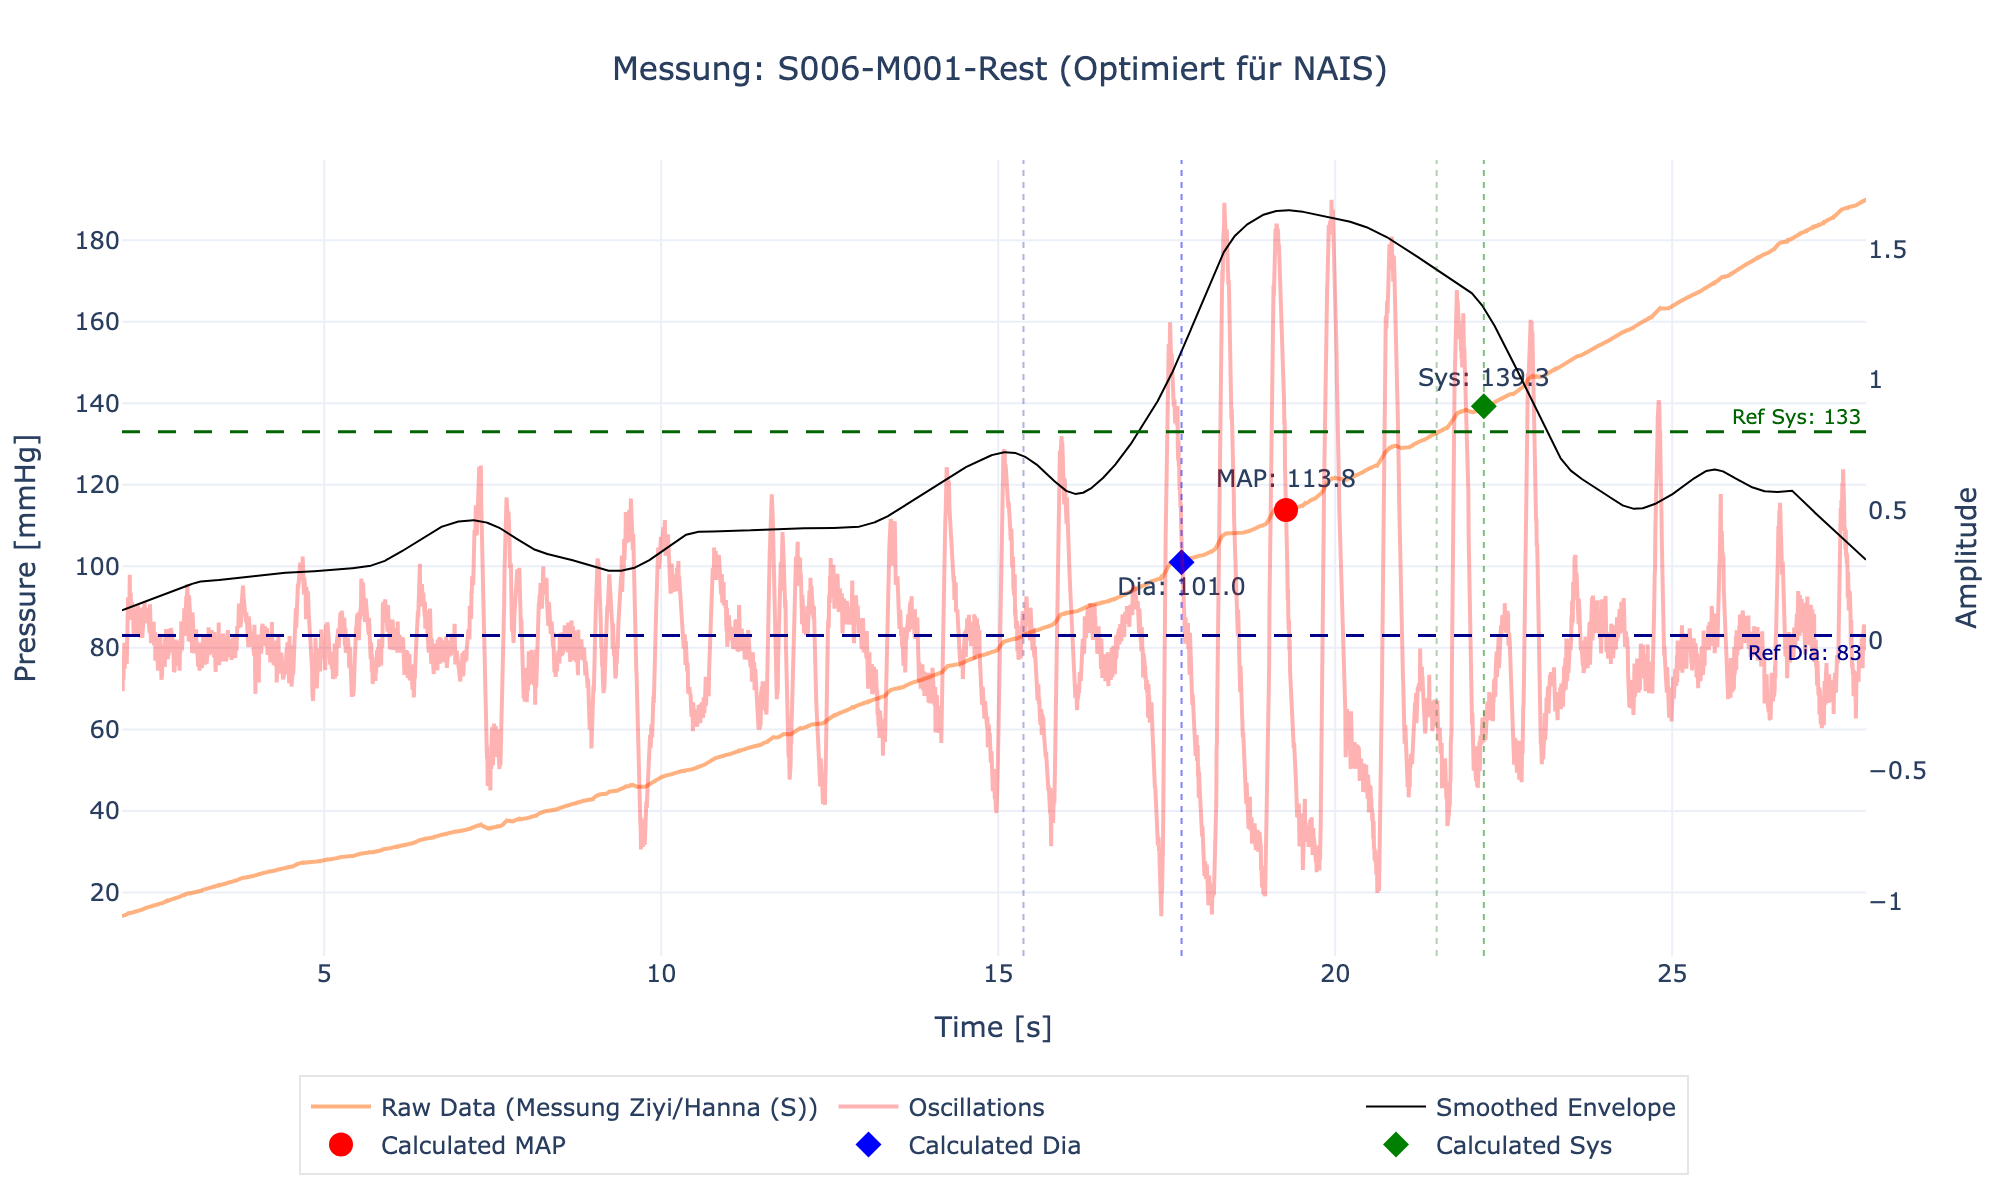
\includegraphics[width=\textwidth]{images/S006-M001-Rest_nais.png}
        \caption{Optimiert für NAIS}
    \end{subfigure}
    \caption{Einzelauswertung der Messung S006-M001-Rest mit verschiedenen Parametersätzen.}
\end{figure}
\newpage

\subsection*{Messung: S006-M002-Active}
\begin{figure}[H]
    \centering
    \begin{subfigure}[b]{0.8\textwidth}
        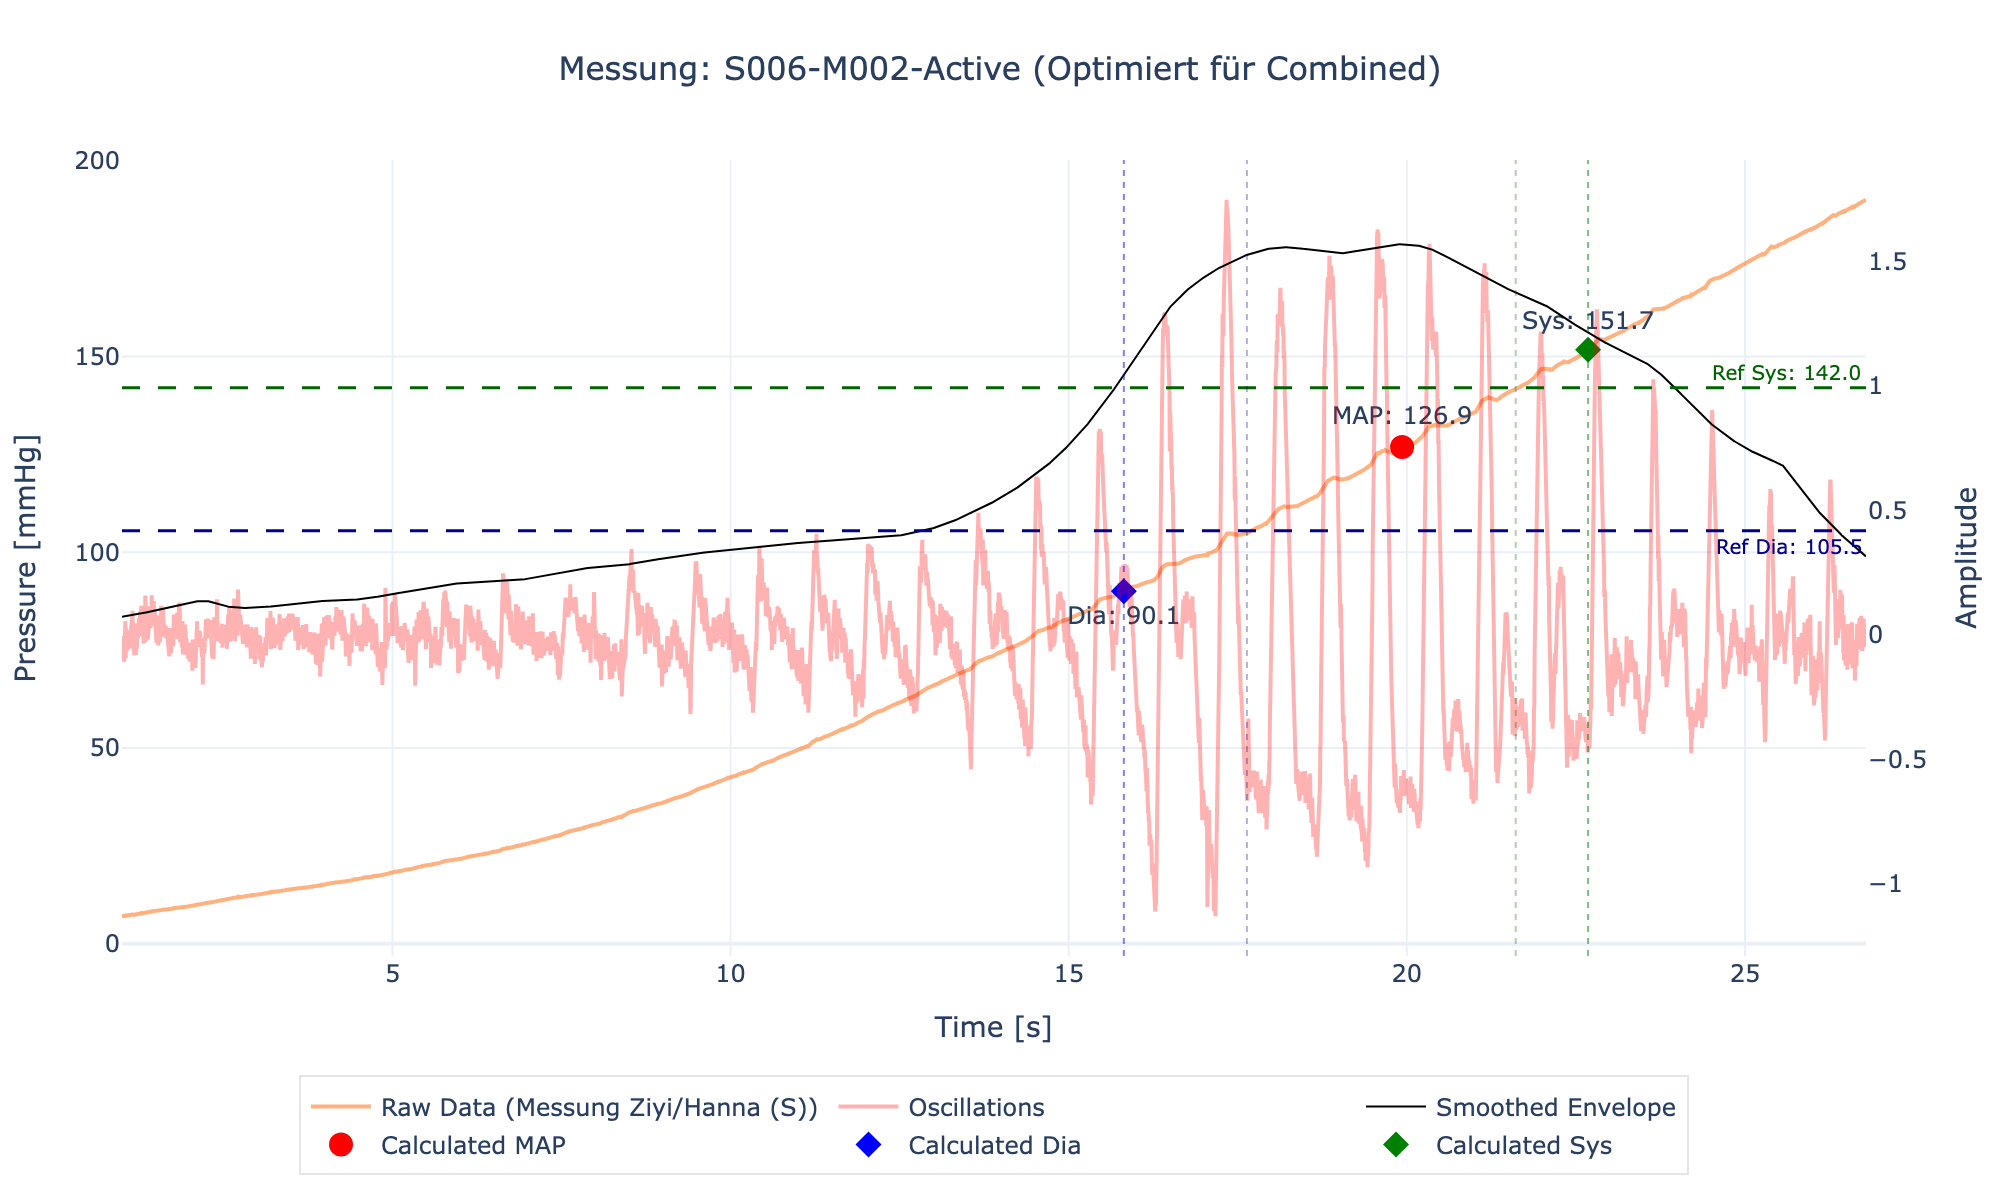
\includegraphics[width=\textwidth]{images/S006-M002-Active_combined.png}
        \caption{Optimiert für Beurer und NAIS (Kombiniert)}
    \end{subfigure} \\
    \begin{subfigure}[b]{0.48\textwidth}
        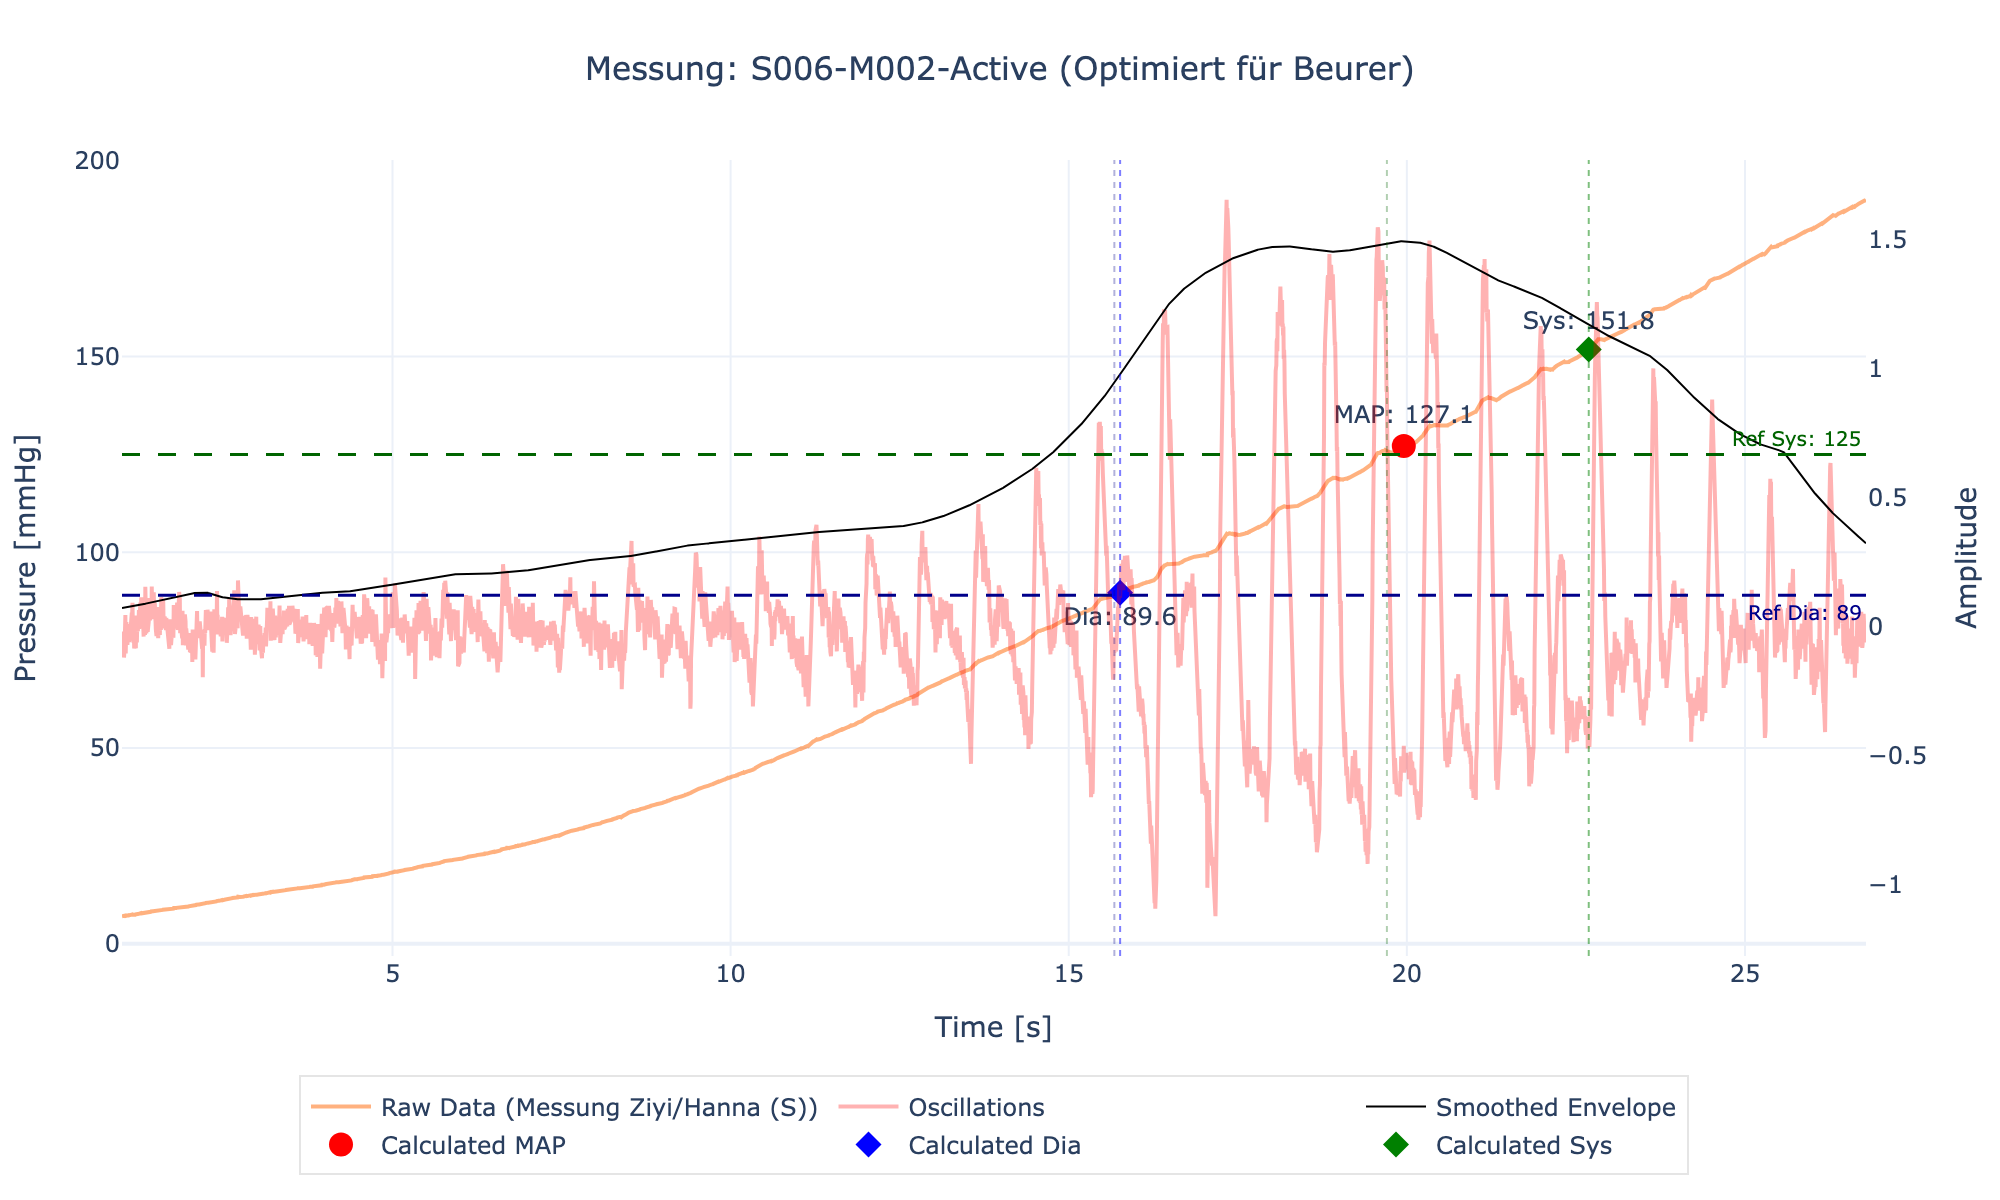
\includegraphics[width=\textwidth]{images/S006-M002-Active_beurer.png}
        \caption{Optimiert für Beurer}
    \end{subfigure}
    \hfill
    \begin{subfigure}[b]{0.48\textwidth}
        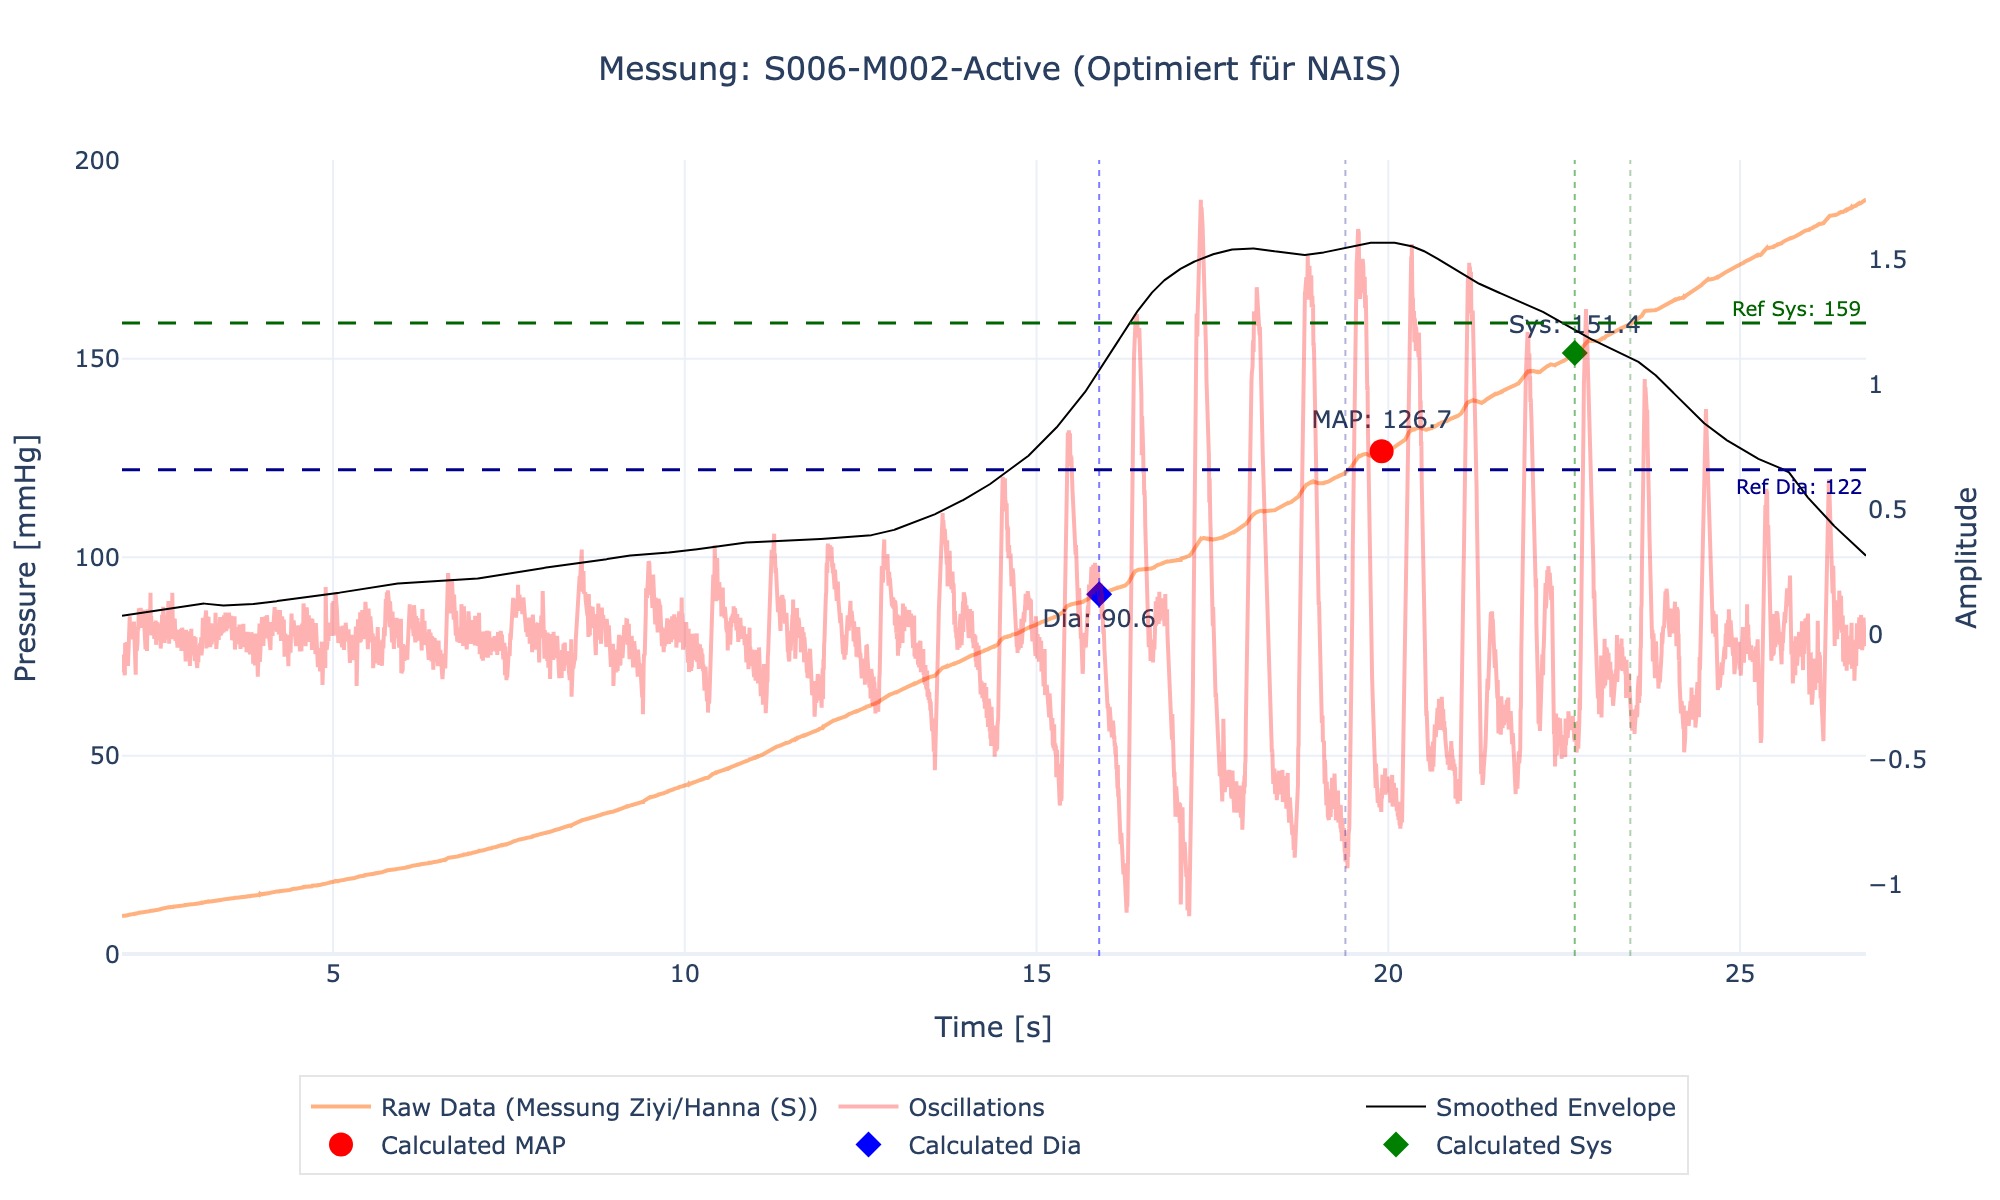
\includegraphics[width=\textwidth]{images/S006-M002-Active_nais.png}
        \caption{Optimiert für NAIS}
    \end{subfigure}
    \caption{Einzelauswertung der Messung S006-M002-Active mit verschiedenen Parametersätzen.}
\end{figure}
\newpage

\subsection*{Messung: S007-M001-Rest}
\begin{figure}[H]
    \centering
    \begin{subfigure}[b]{0.8\textwidth}
        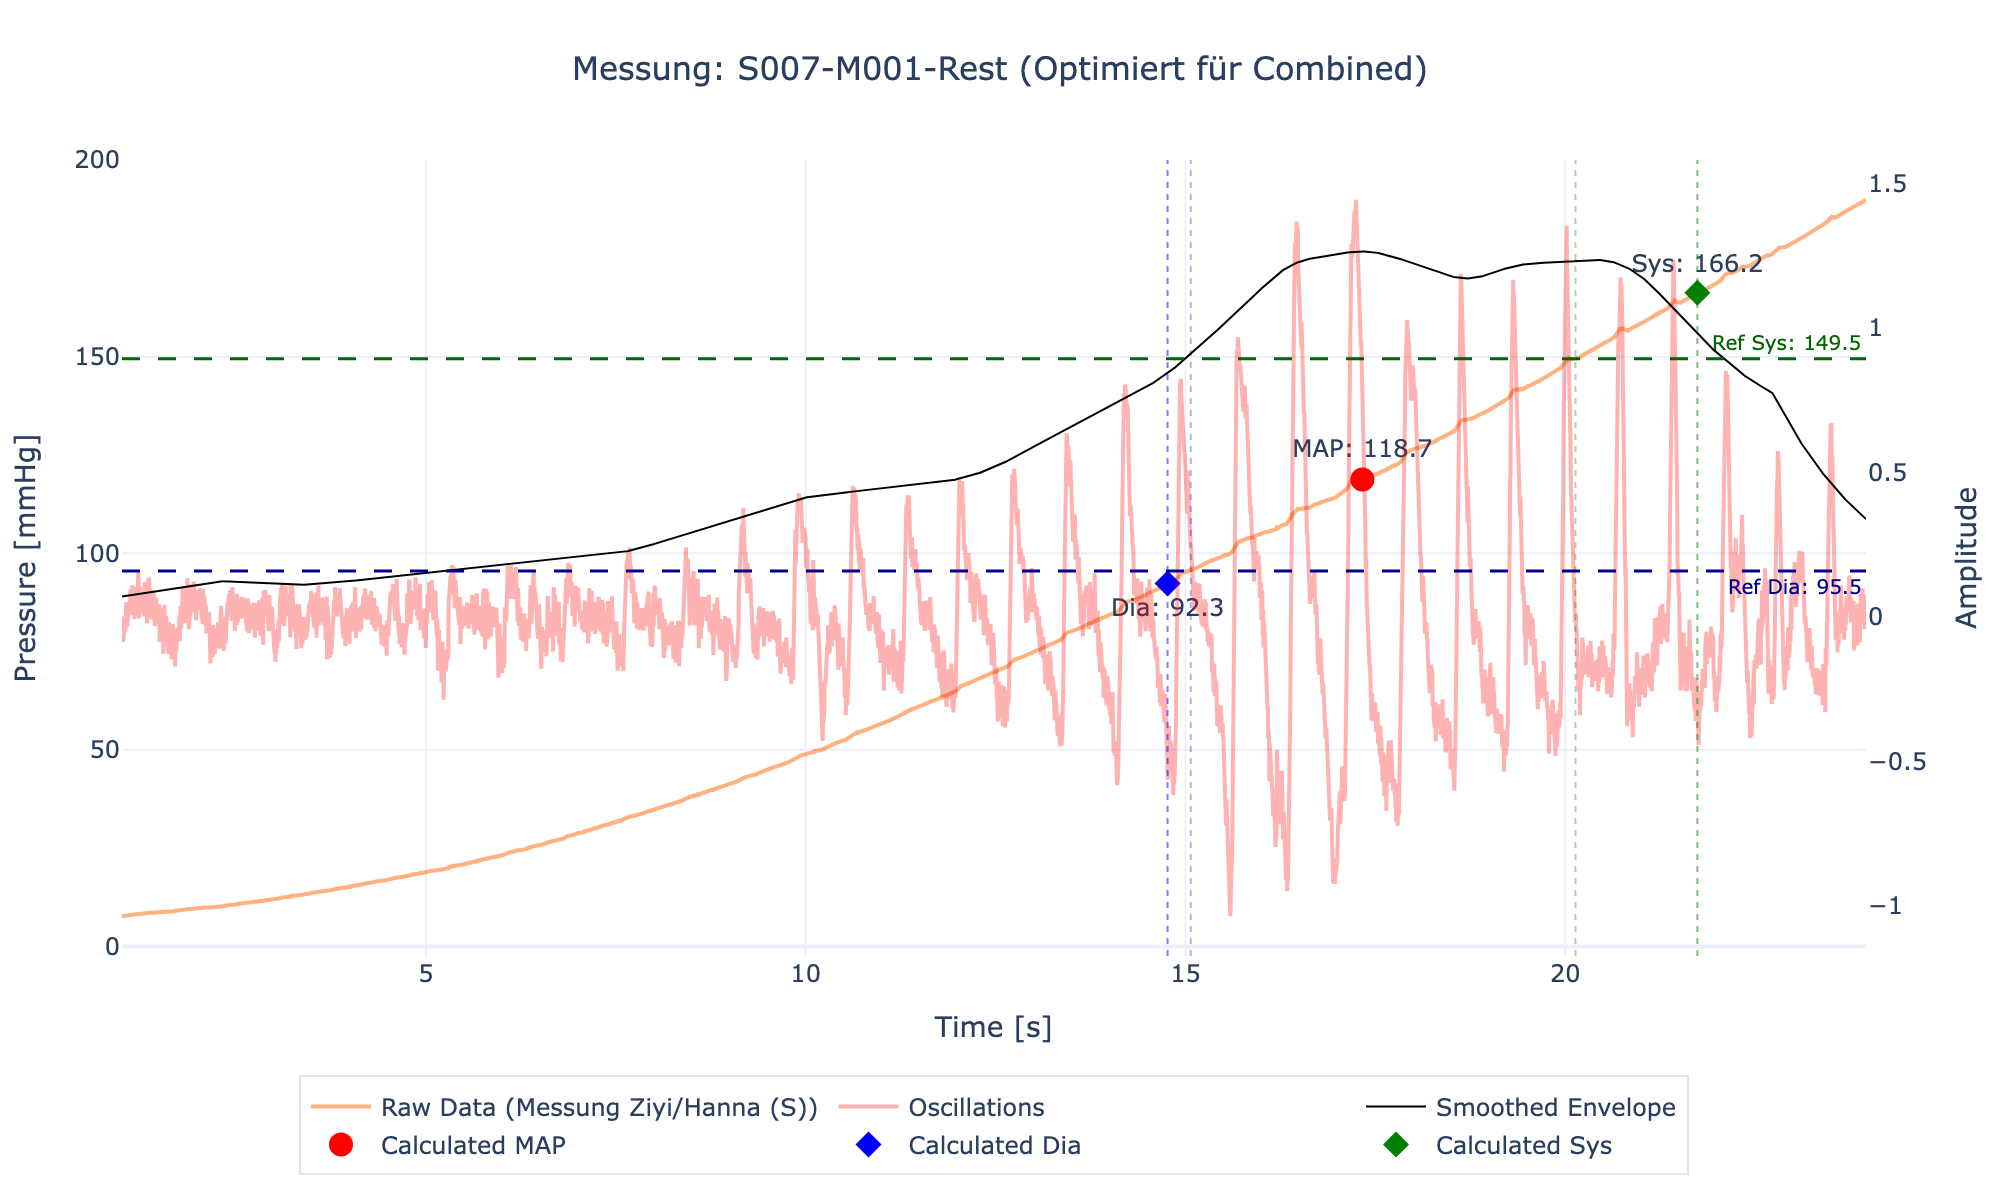
\includegraphics[width=\textwidth]{images/S007-M001-Rest_combined.png}
        \caption{Optimiert für Beurer und NAIS (Kombiniert)}
    \end{subfigure} \\
    \begin{subfigure}[b]{0.48\textwidth}
        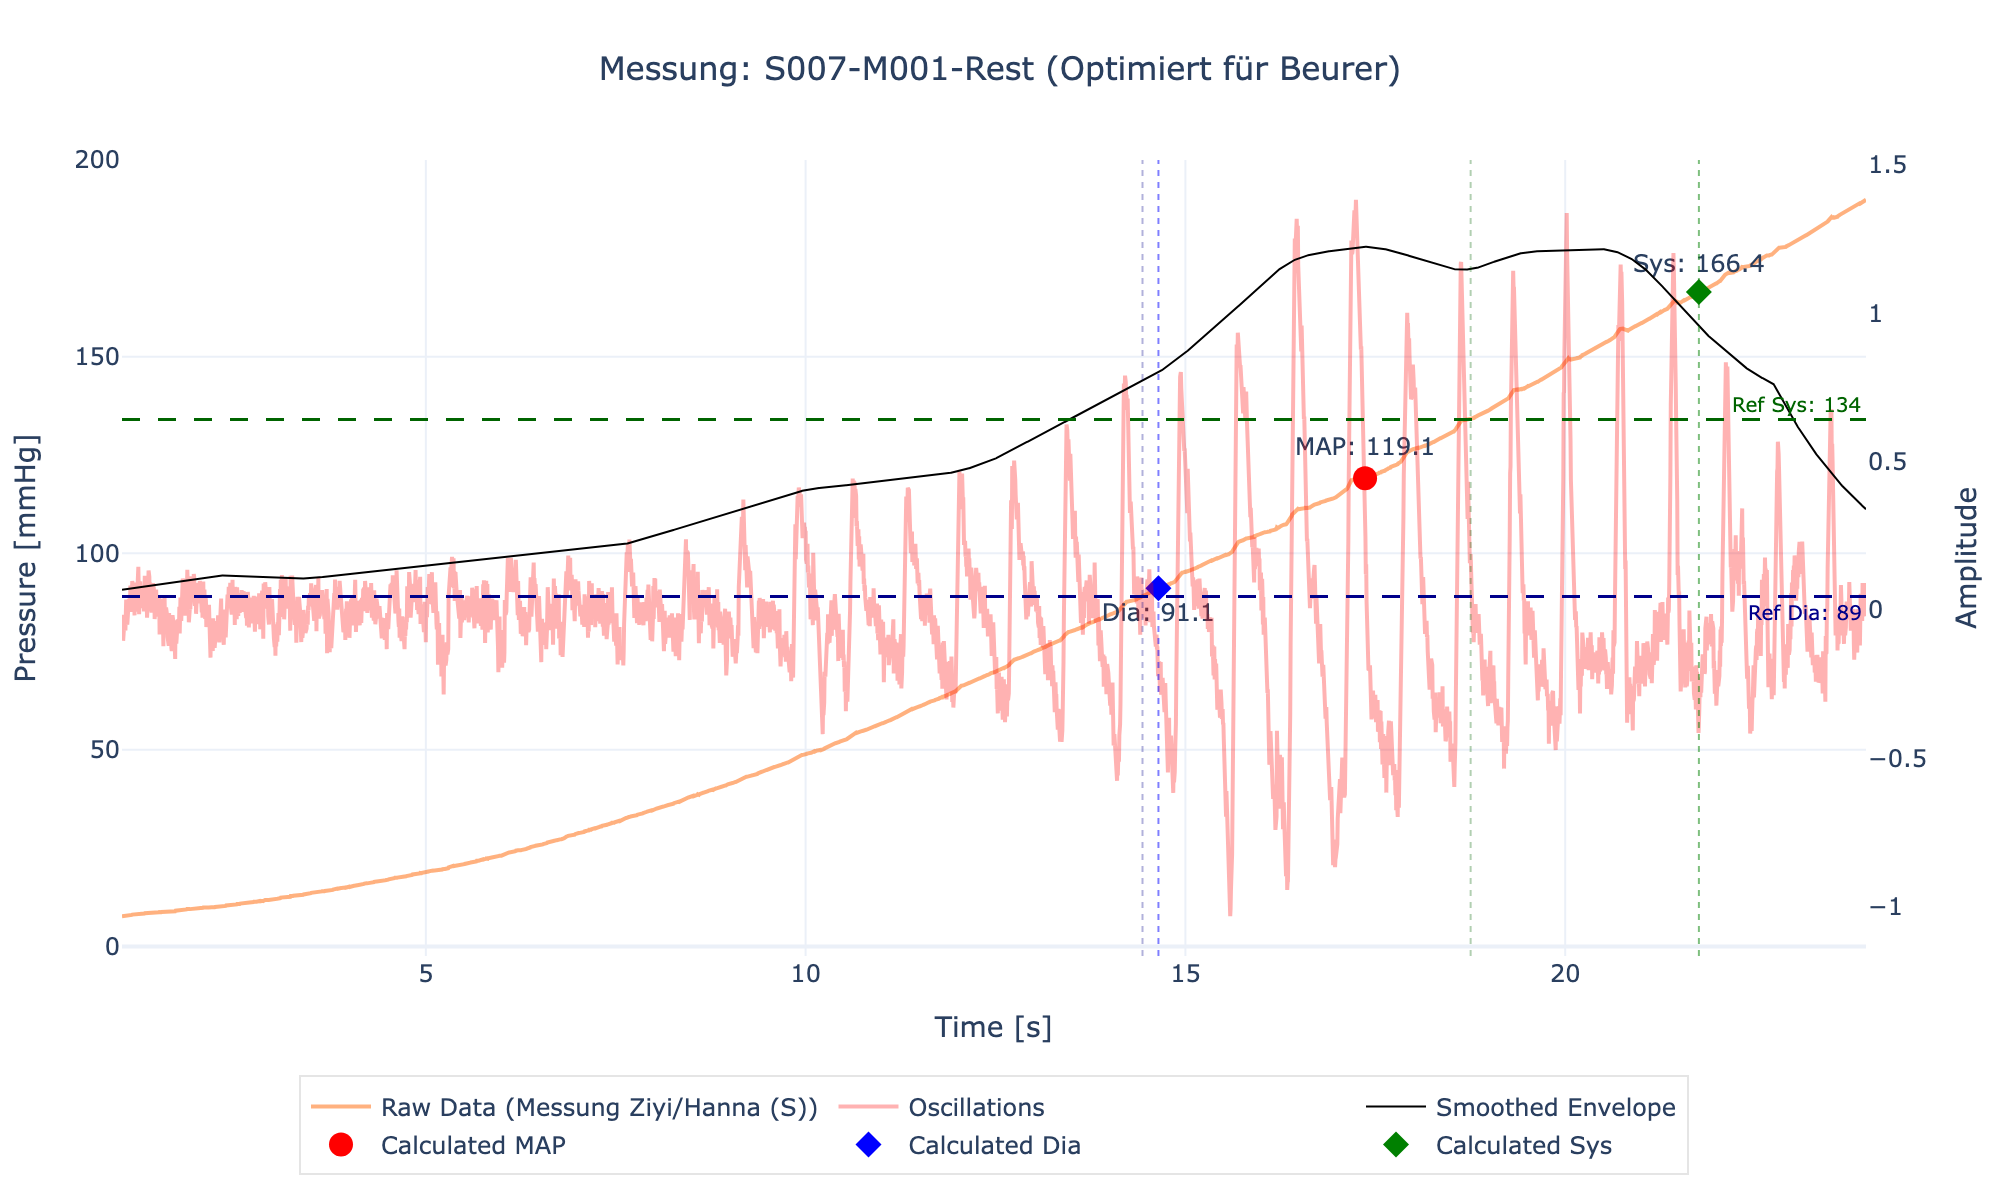
\includegraphics[width=\textwidth]{images/S007-M001-Rest_beurer.png}
        \caption{Optimiert für Beurer}
    \end{subfigure}
    \hfill
    \begin{subfigure}[b]{0.48\textwidth}
        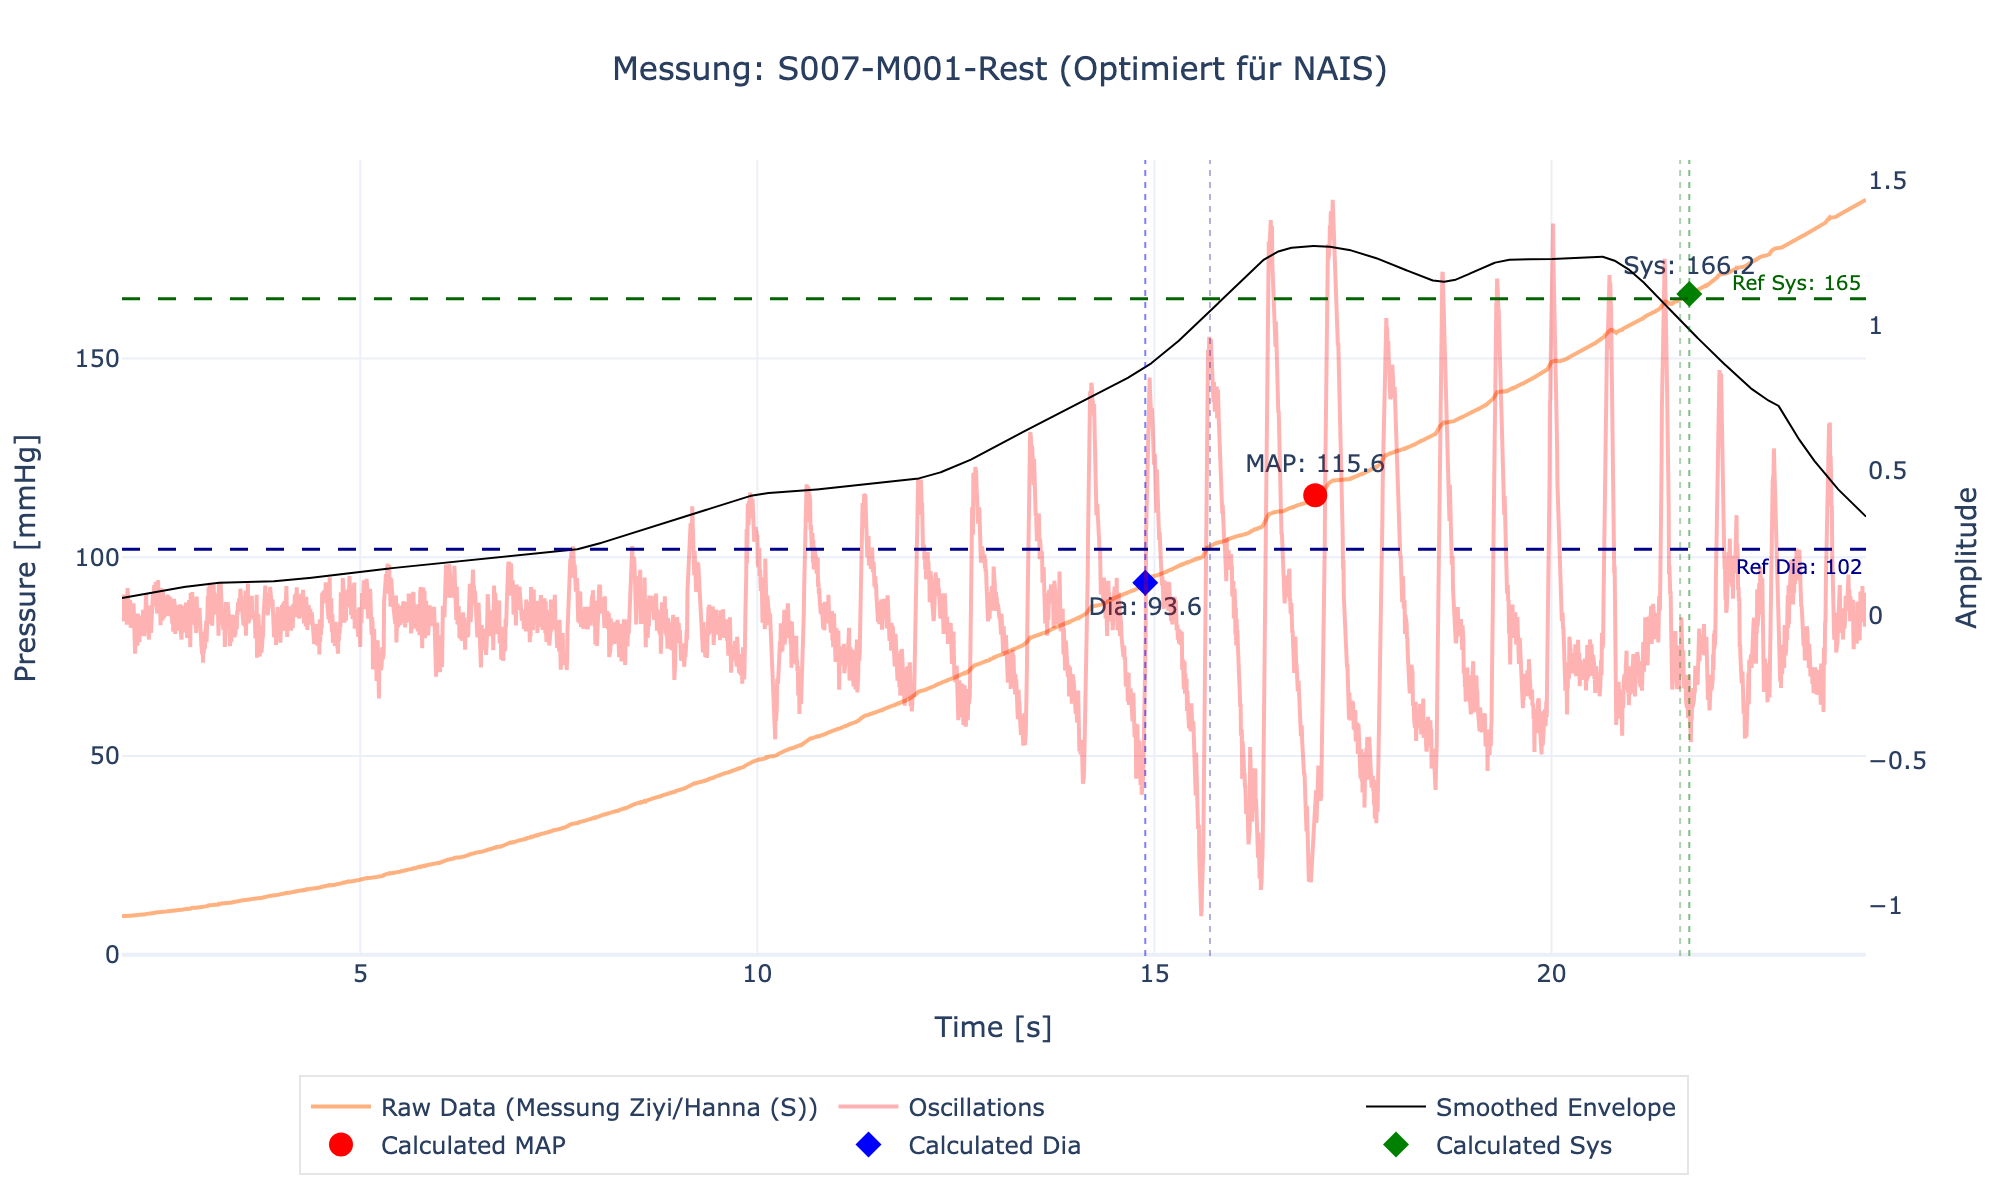
\includegraphics[width=\textwidth]{images/S007-M001-Rest_nais.png}
        \caption{Optimiert für NAIS}
    \end{subfigure}
    \caption{Einzelauswertung der Messung S007-M001-Rest mit verschiedenen Parametersätzen.}
\end{figure}
\newpage

\subsection*{Messung: S007-M002-Active}
\begin{figure}[H]
    \centering
    \begin{subfigure}[b]{0.8\textwidth}
        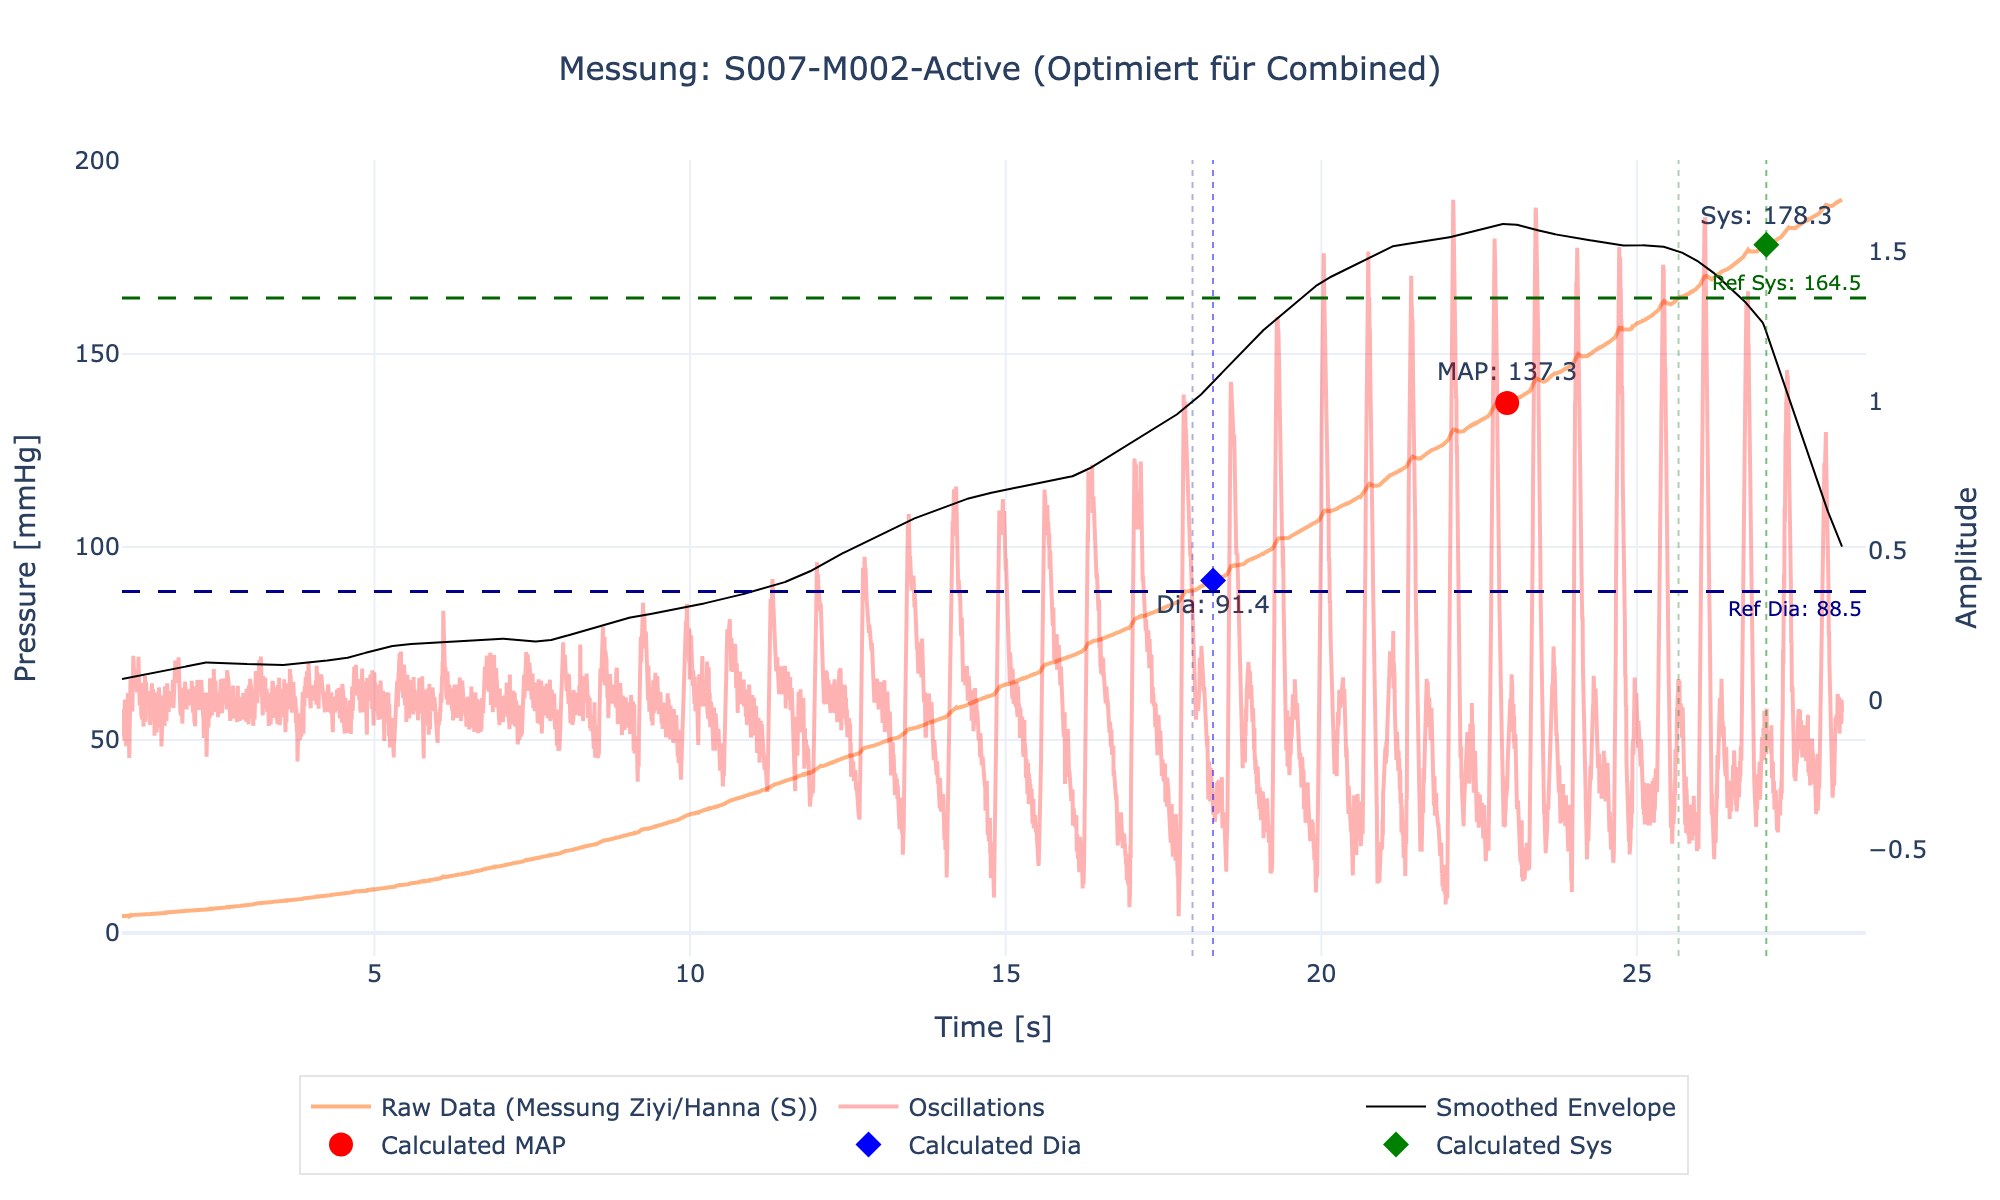
\includegraphics[width=\textwidth]{images/S007-M002-Active_combined.png}
        \caption{Optimiert für Beurer und NAIS (Kombiniert)}
    \end{subfigure} \\
    \begin{subfigure}[b]{0.48\textwidth}
        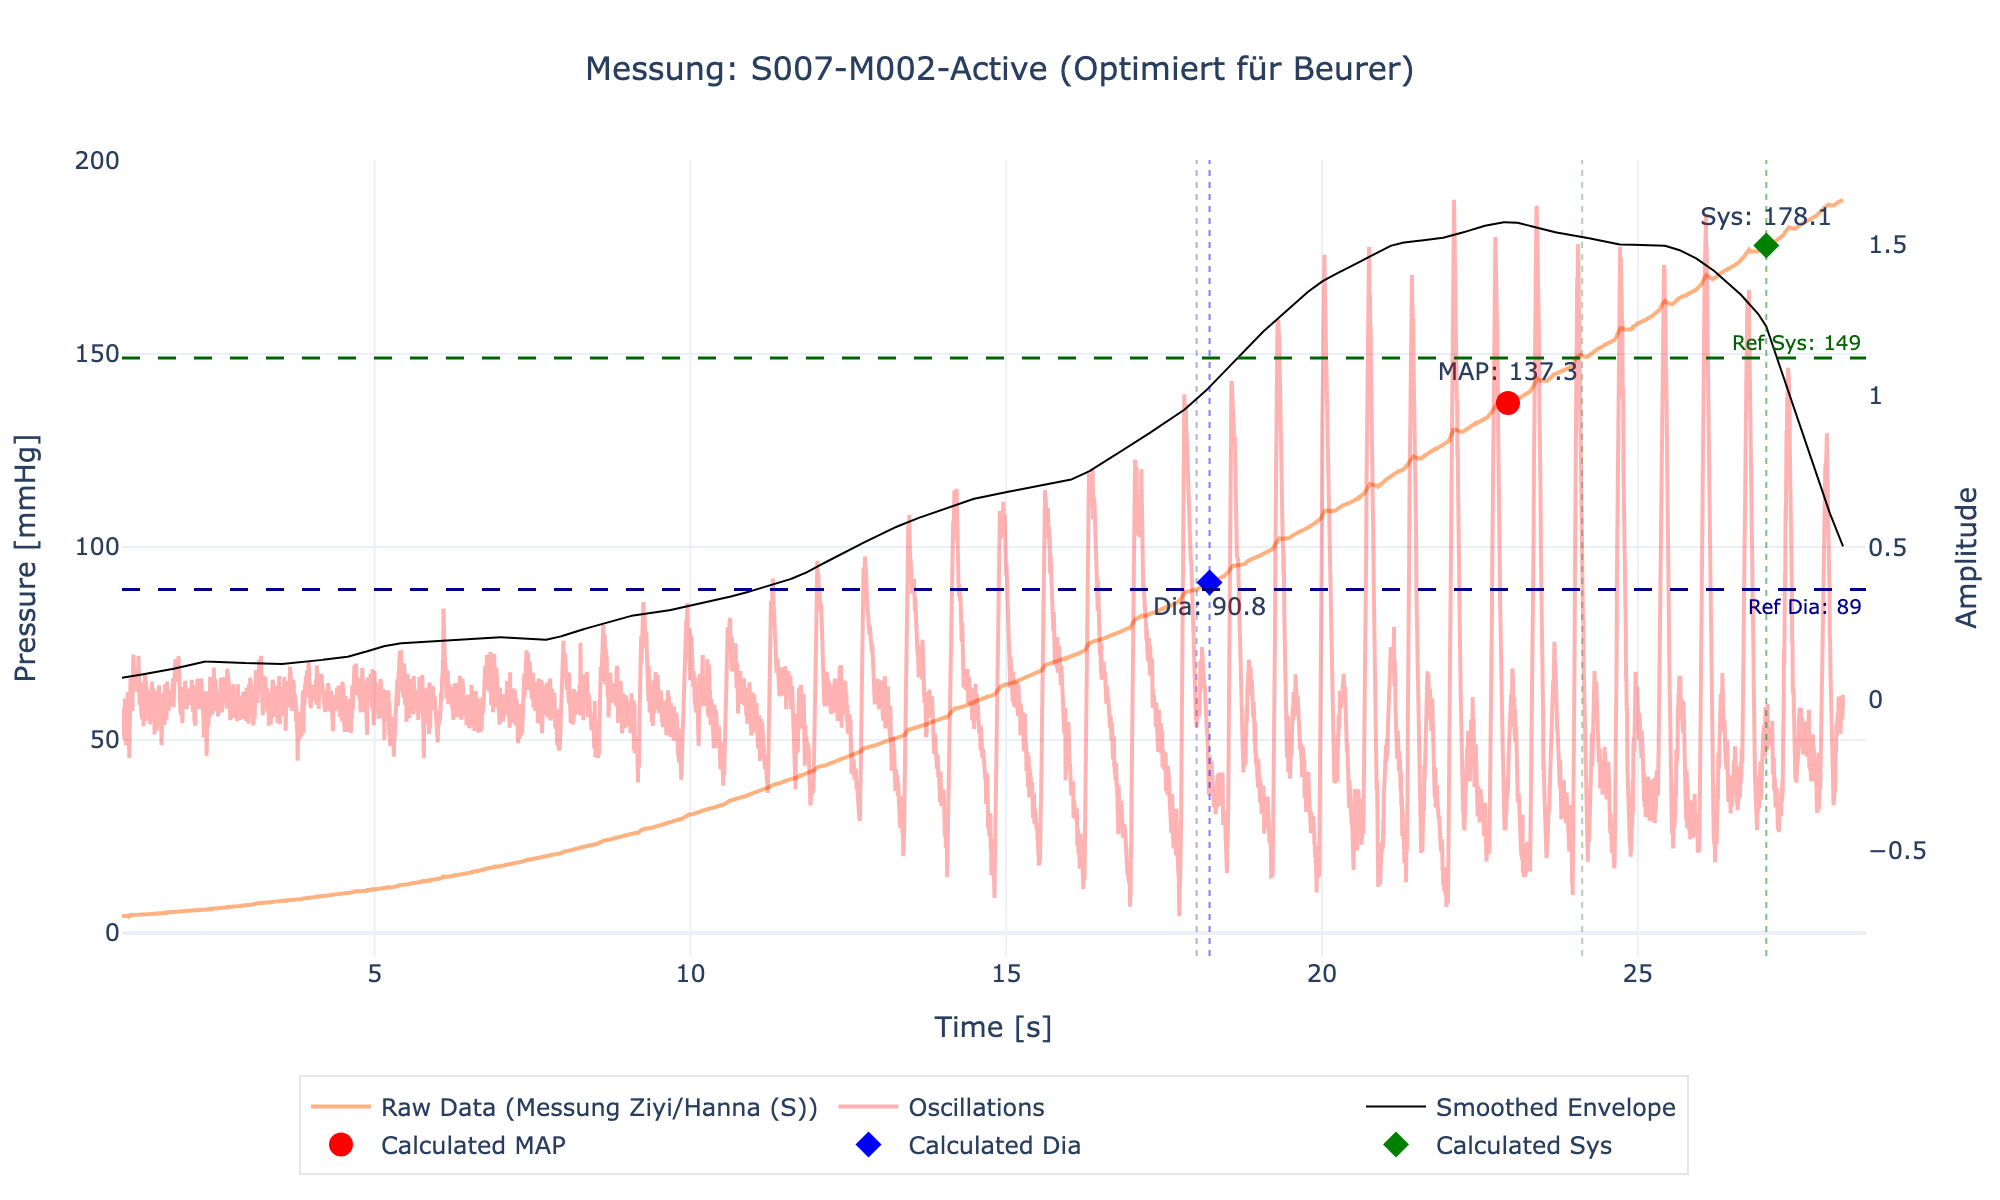
\includegraphics[width=\textwidth]{images/S007-M002-Active_beurer.png}
        \caption{Optimiert für Beurer}
    \end{subfigure}
    \hfill
    \begin{subfigure}[b]{0.48\textwidth}
        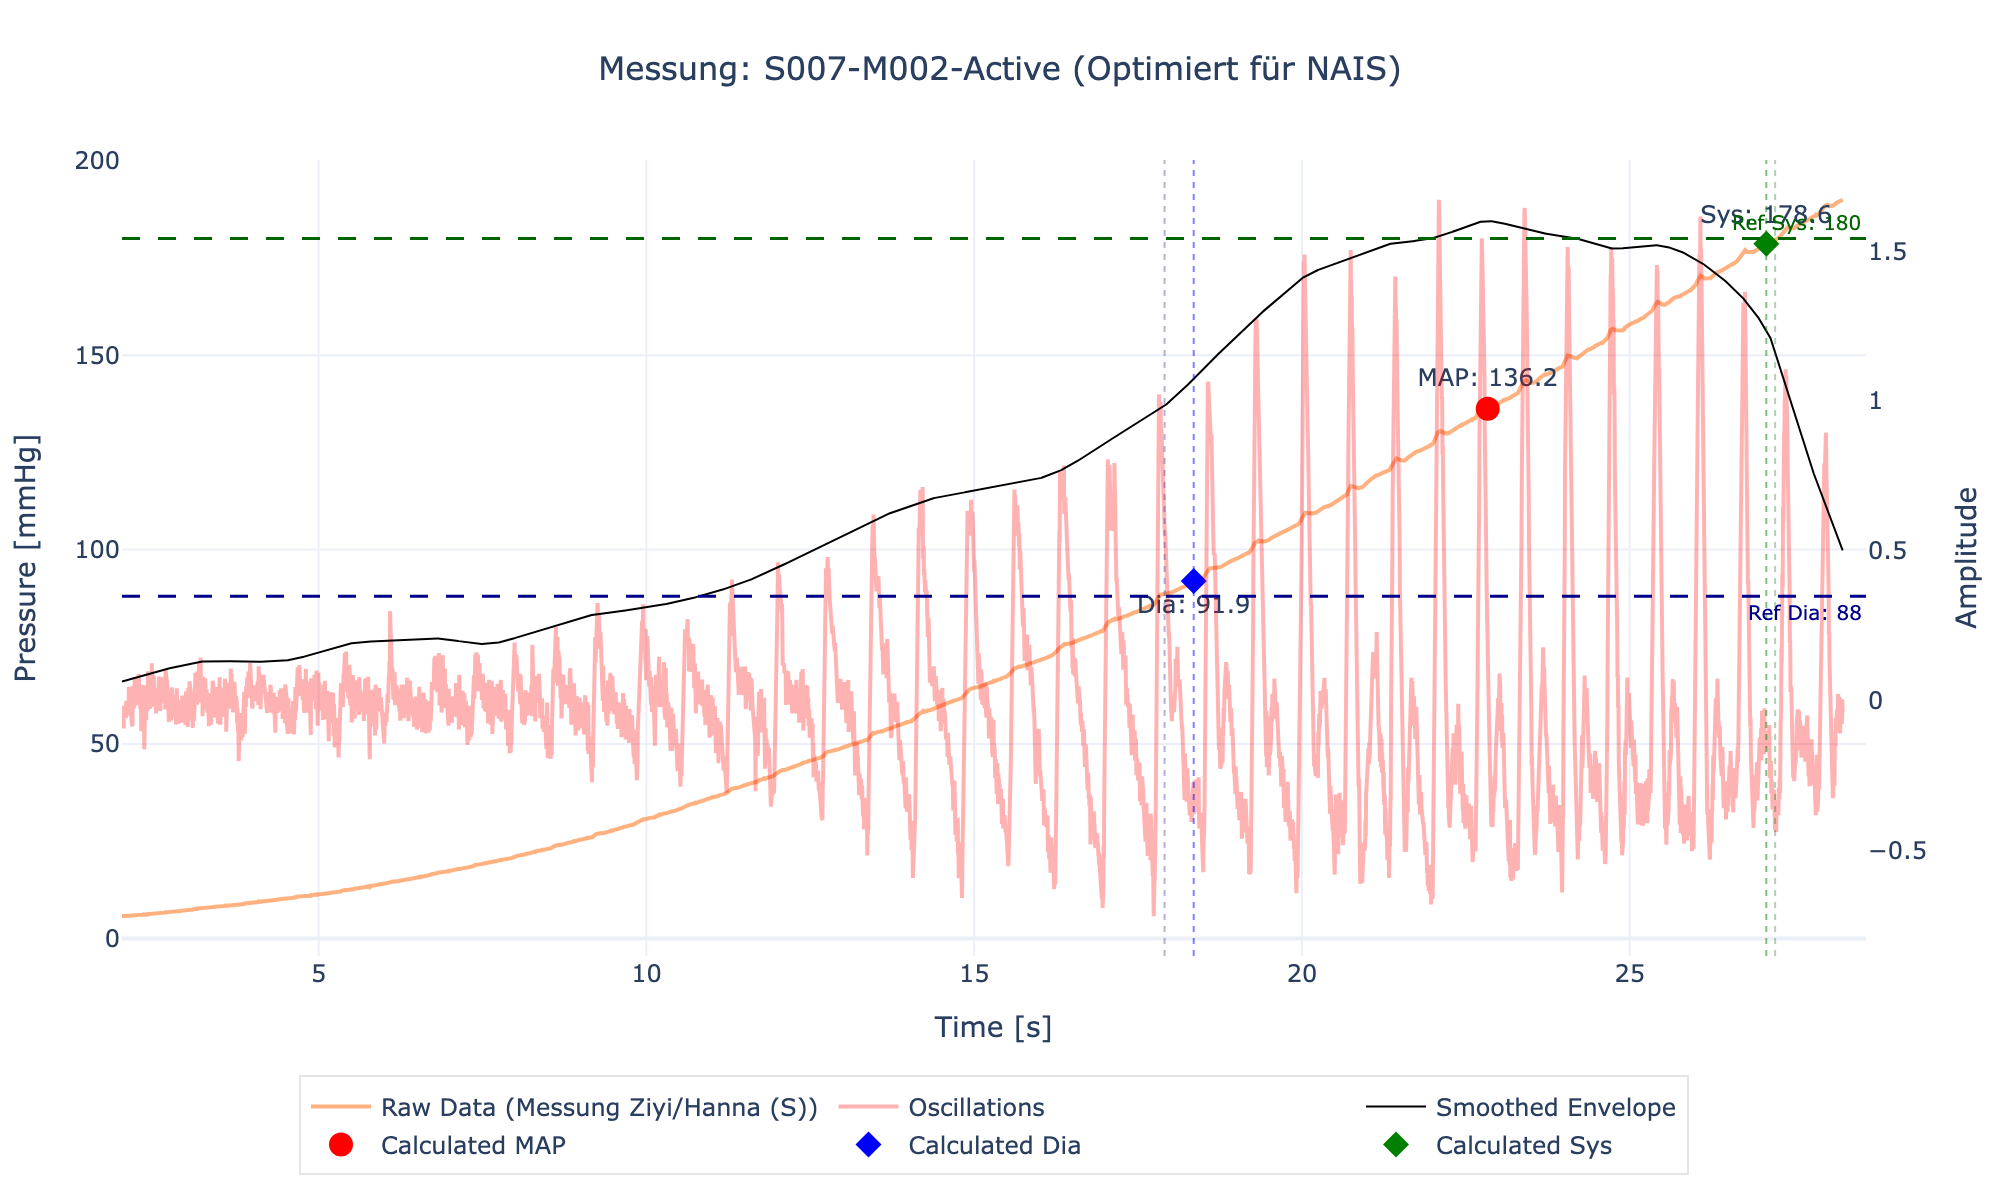
\includegraphics[width=\textwidth]{images/S007-M002-Active_nais.png}
        \caption{Optimiert für NAIS}
    \end{subfigure}
    \caption{Einzelauswertung der Messung S007-M002-Active mit verschiedenen Parametersätzen.}
\end{figure}
\newpage

\subsection*{Messung: S008-M001-Rest}
\begin{figure}[H]
    \centering
    \begin{subfigure}[b]{0.8\textwidth}
        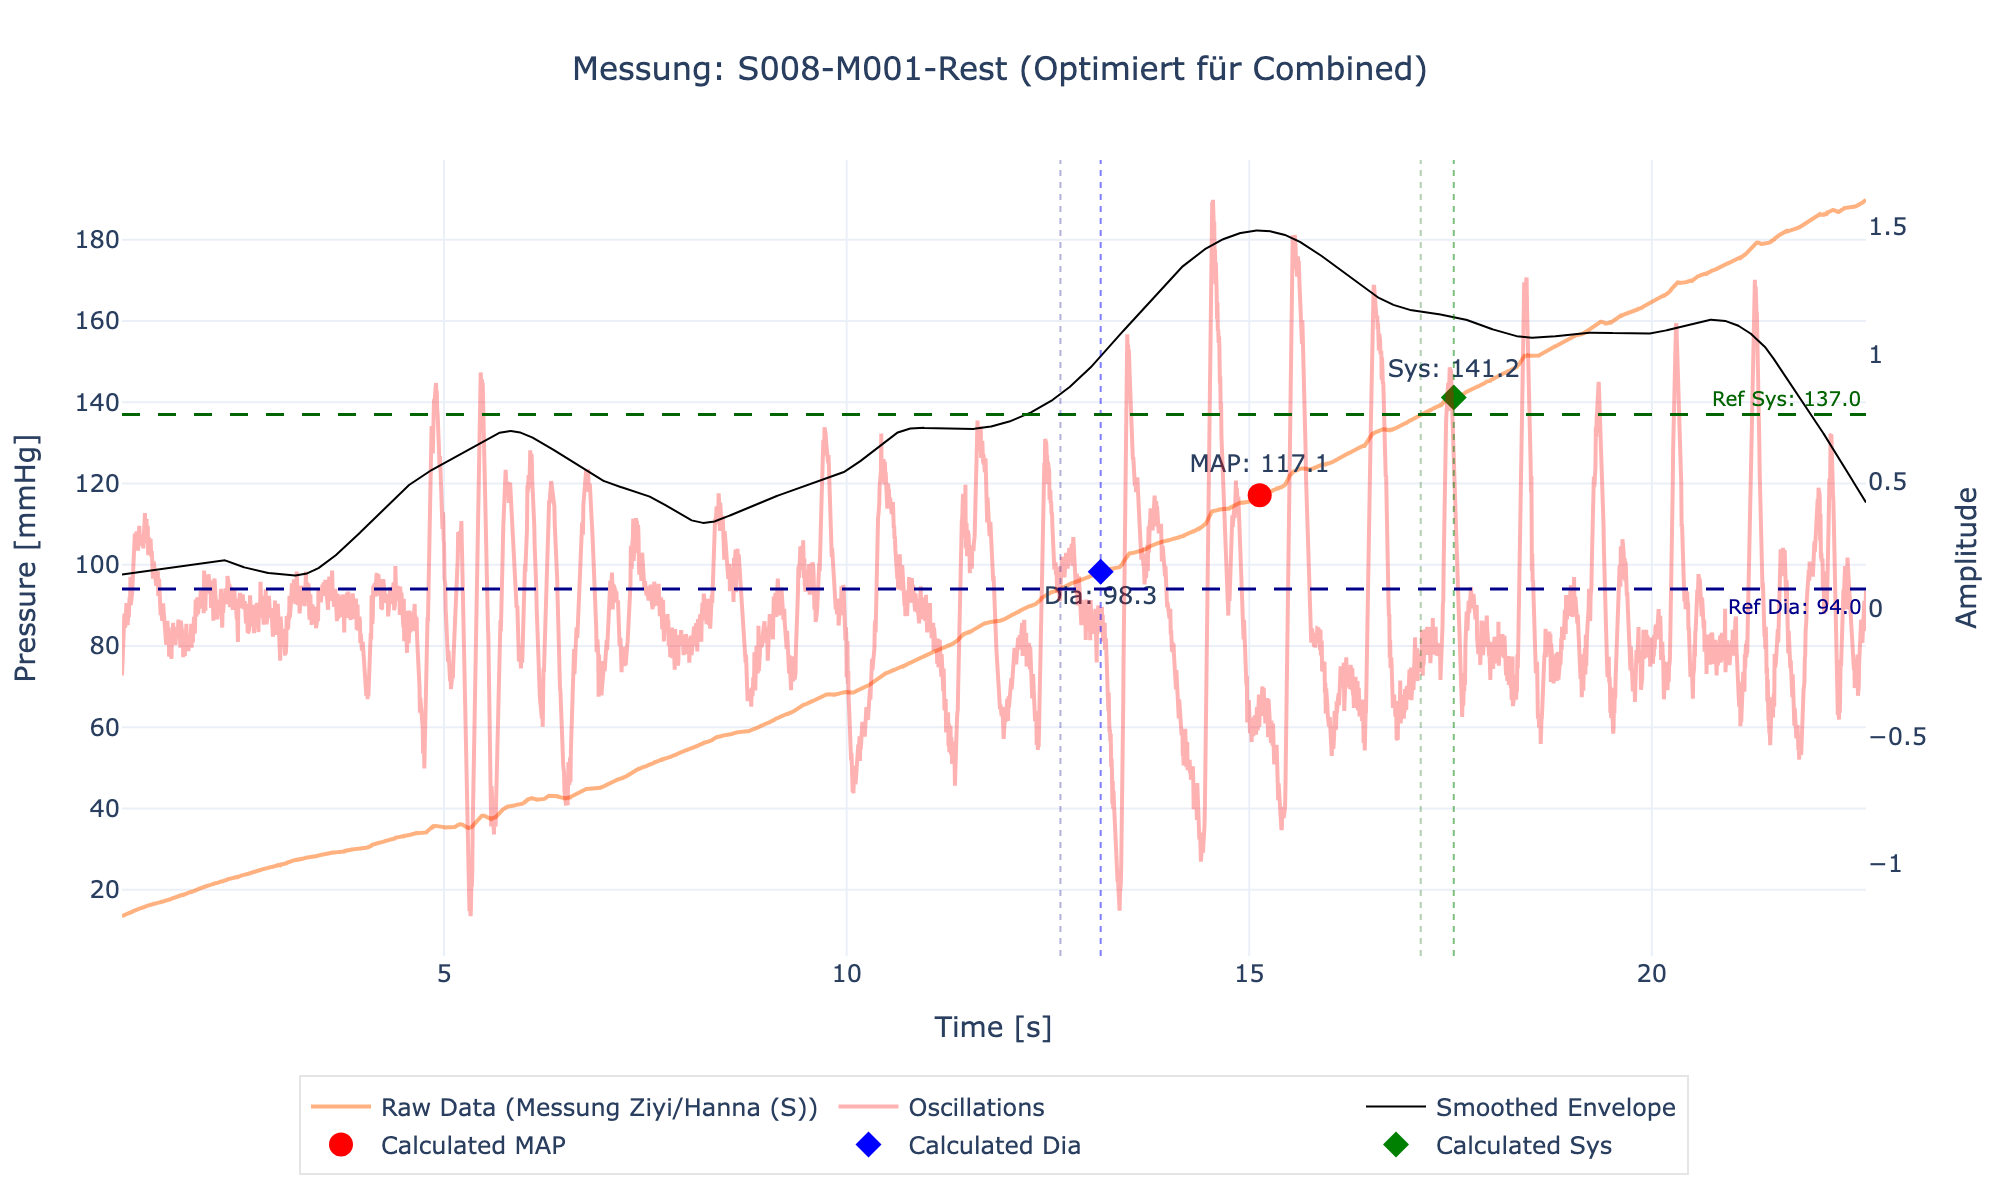
\includegraphics[width=\textwidth]{images/S008-M001-Rest_combined.png}
        \caption{Optimiert für Beurer und NAIS (Kombiniert)}
    \end{subfigure} \\
    \begin{subfigure}[b]{0.48\textwidth}
        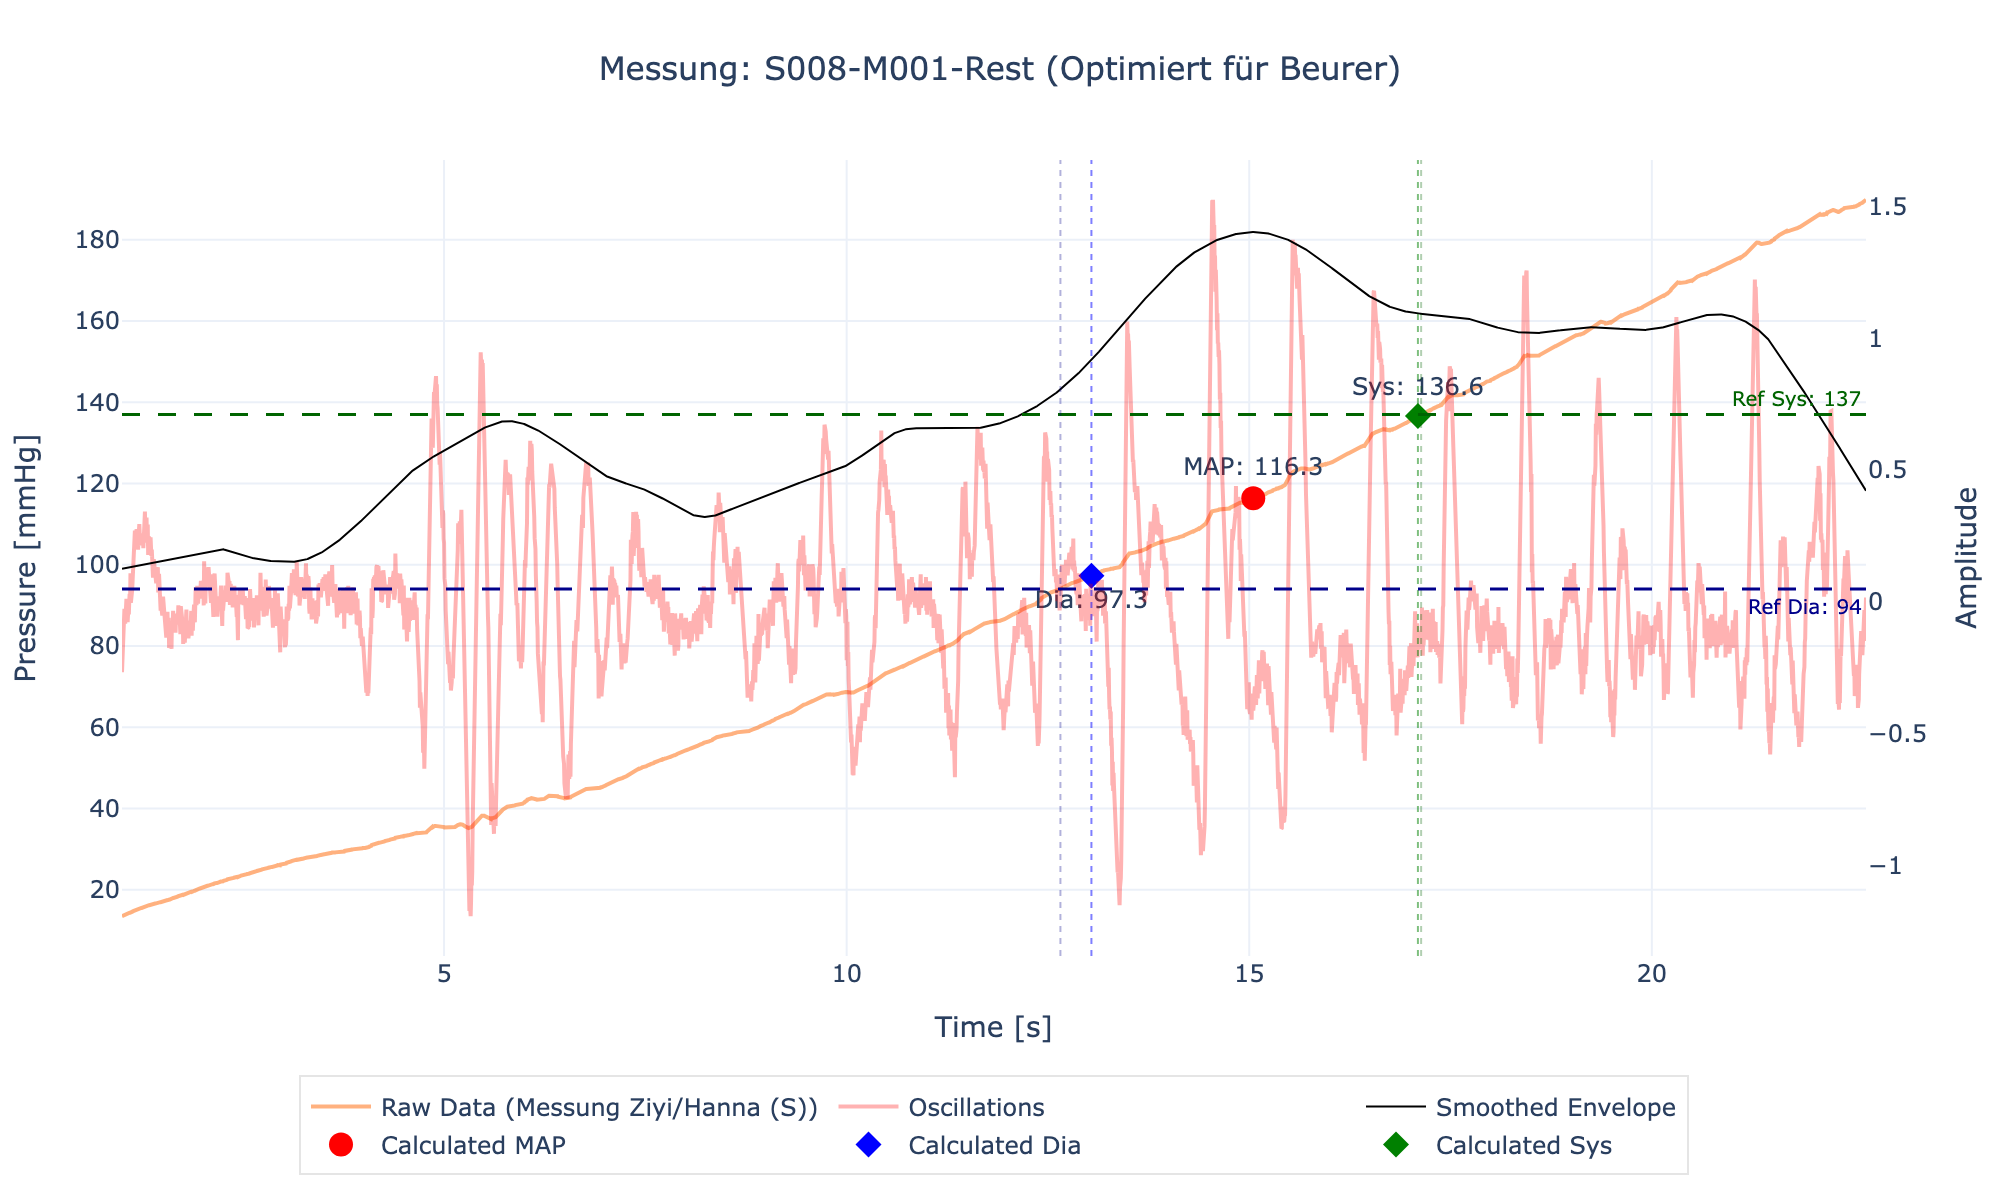
\includegraphics[width=\textwidth]{images/S008-M001-Rest_beurer.png}
        \caption{Optimiert für Beurer}
    \end{subfigure}
    \hfill
    \begin{subfigure}[b]{0.48\textwidth}
        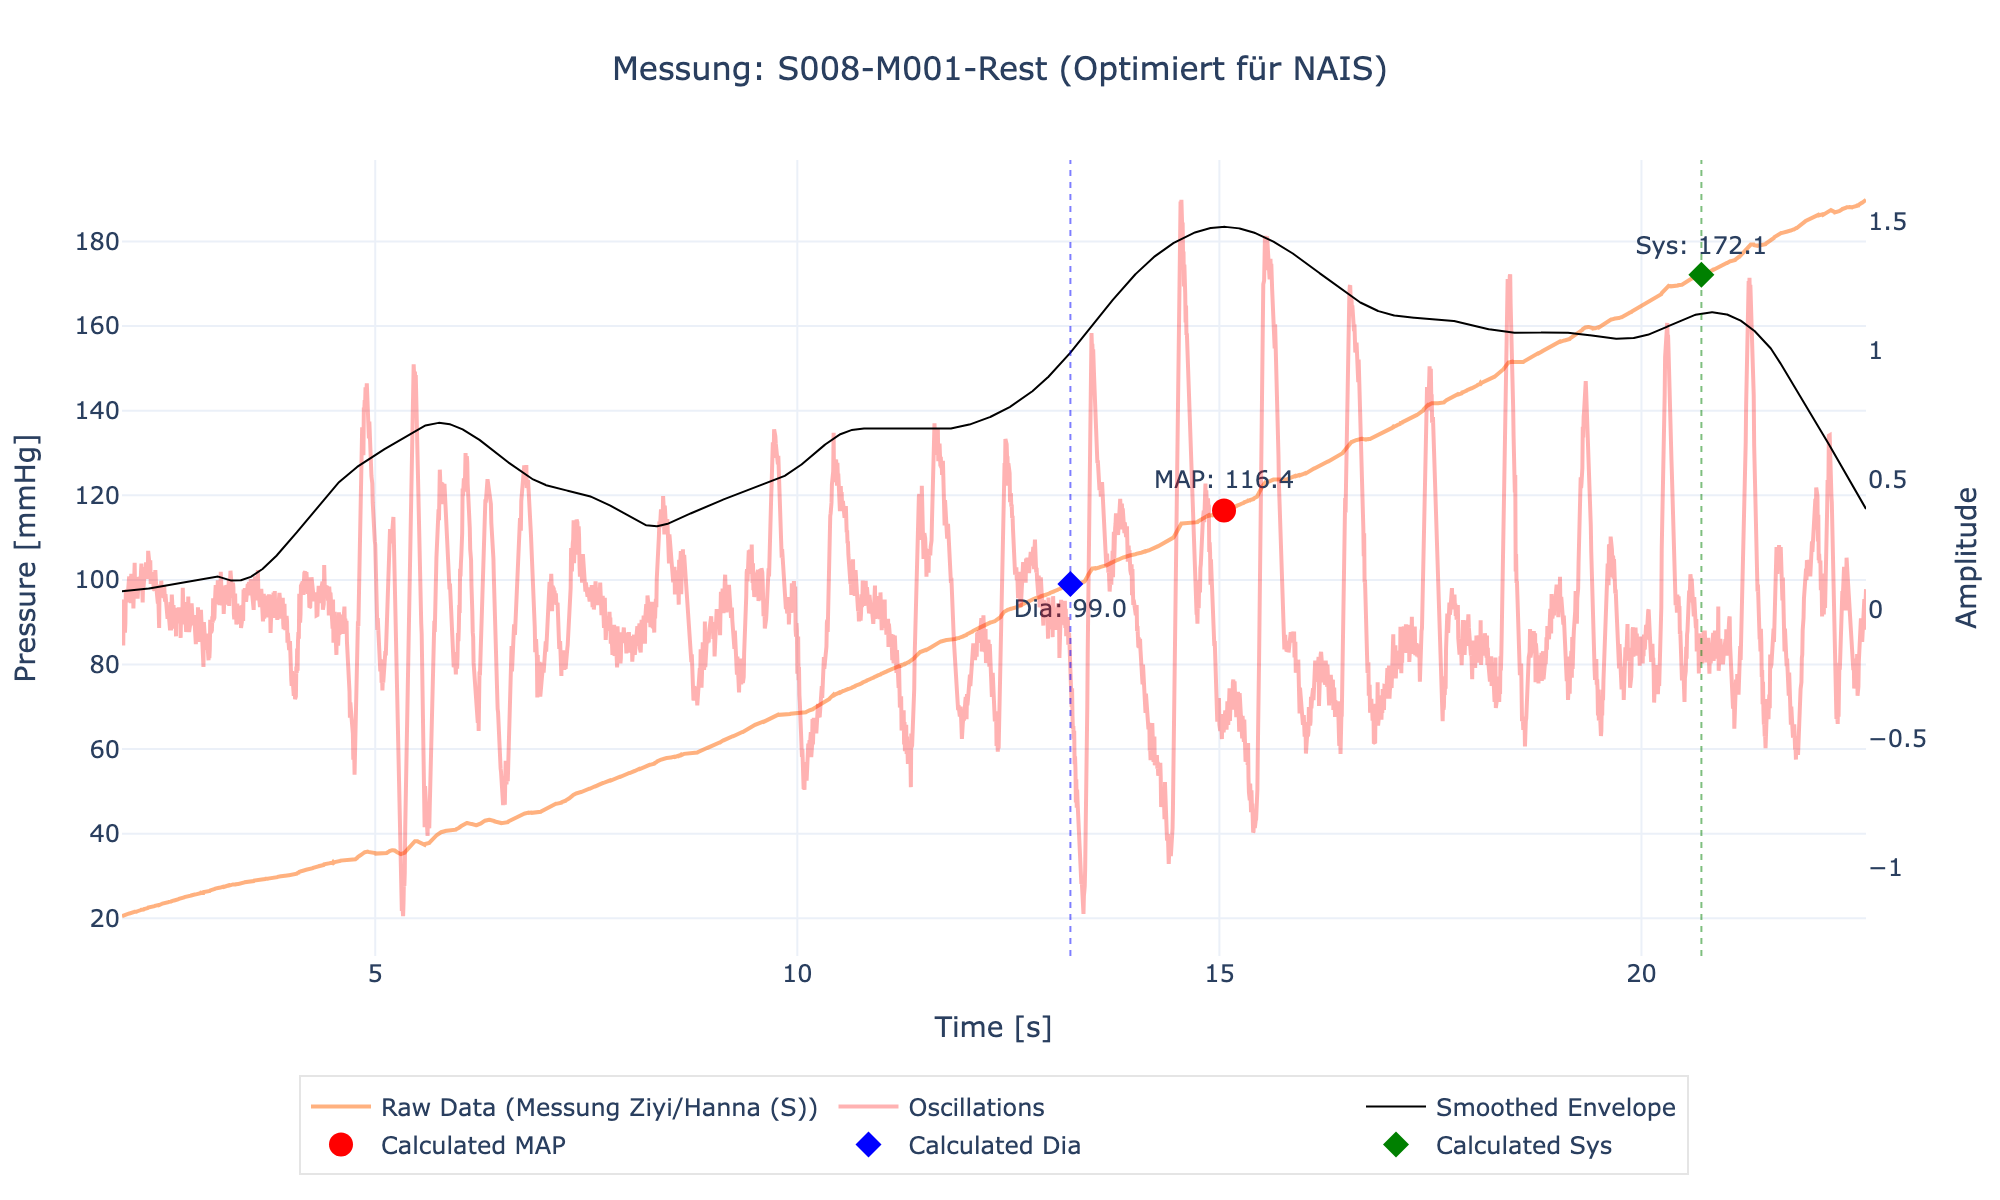
\includegraphics[width=\textwidth]{images/S008-M001-Rest_nais.png}
        \caption{Optimiert für NAIS}
    \end{subfigure}
    \caption{Einzelauswertung der Messung S008-M001-Rest mit verschiedenen Parametersätzen.}
\end{figure}
\newpage

\subsection*{Messung: S008-M002-Active}
\begin{figure}[H]
    \centering
    \begin{subfigure}[b]{0.8\textwidth}
        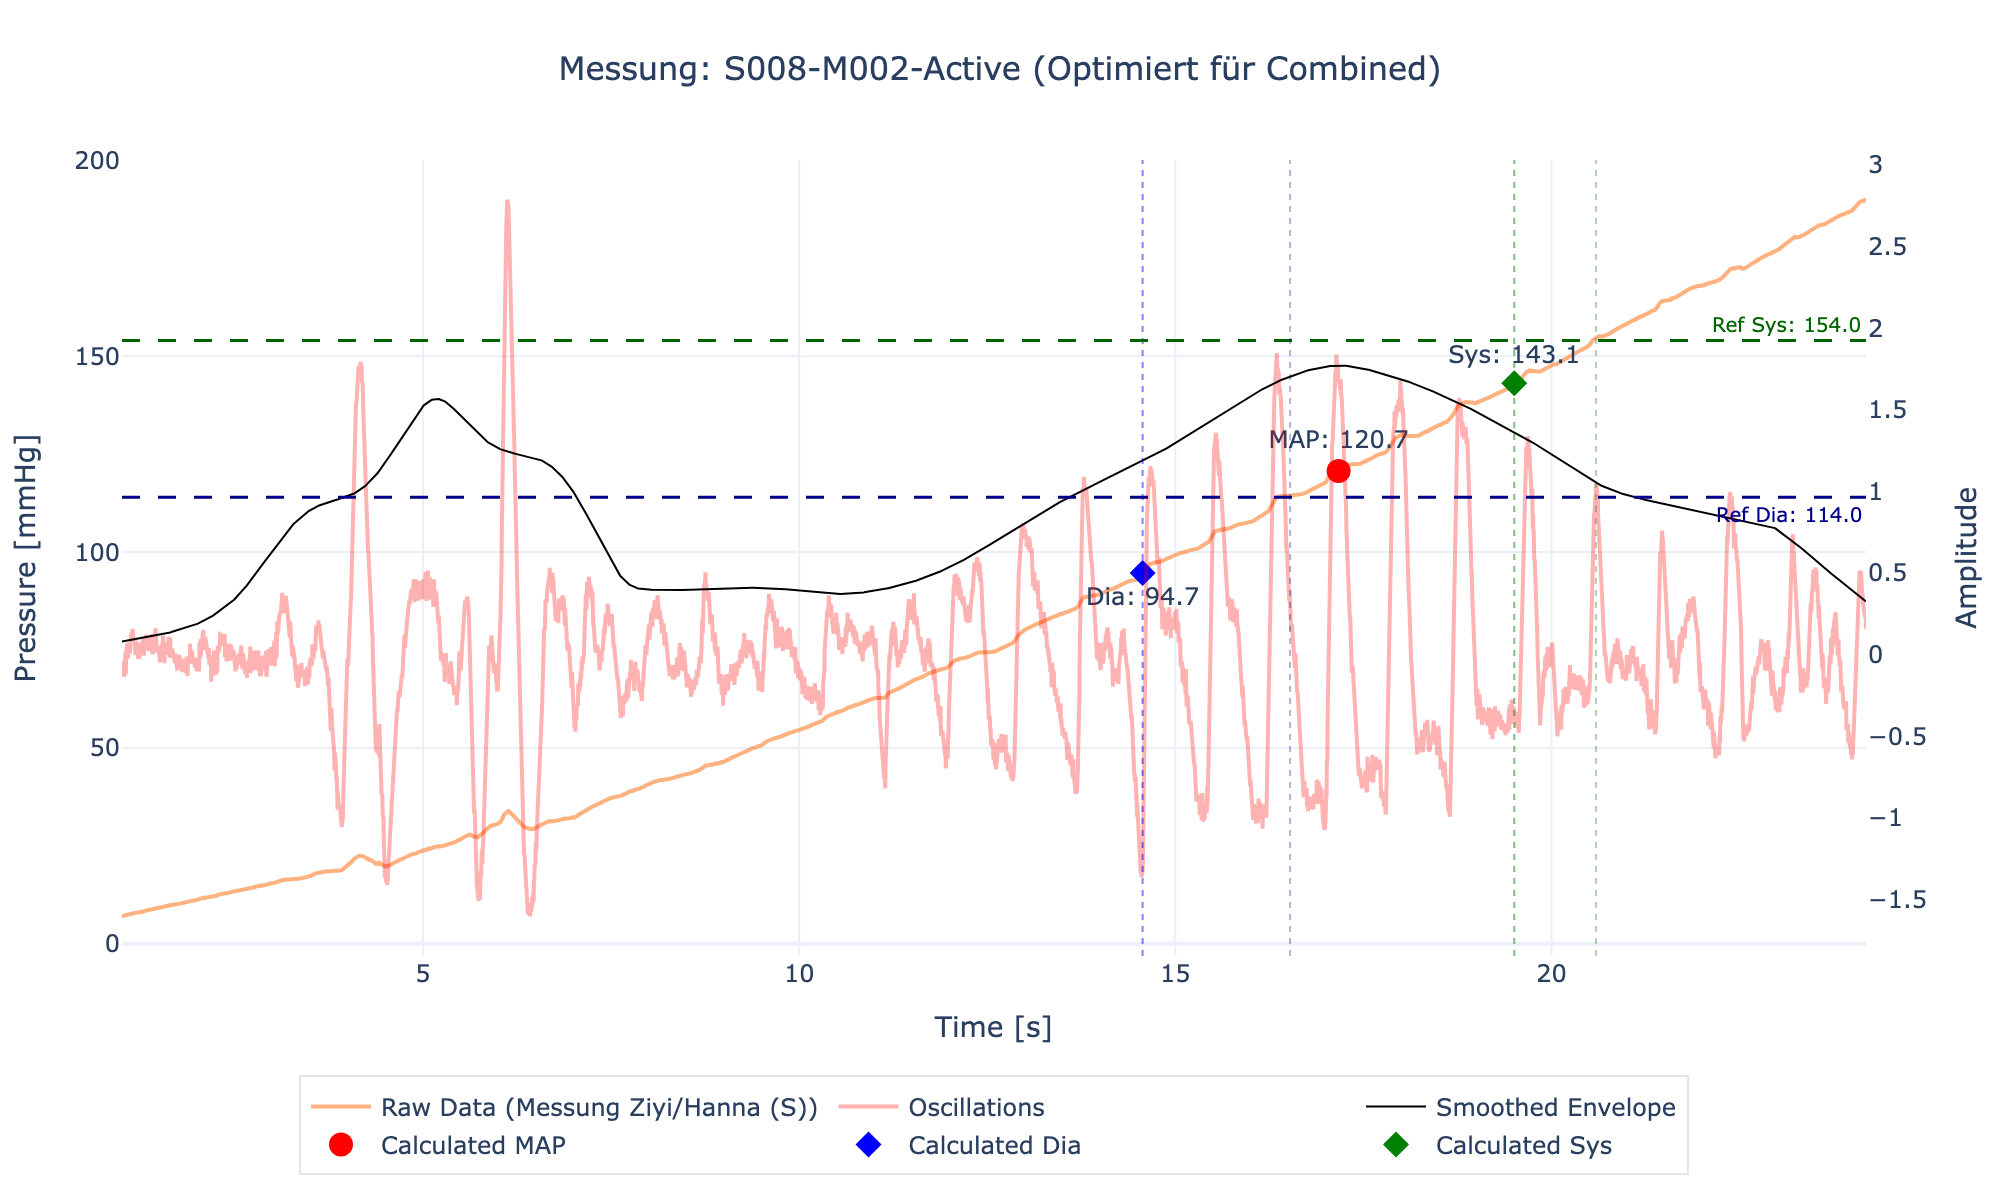
\includegraphics[width=\textwidth]{images/S008-M002-Active_combined.png}
        \caption{Optimiert für Beurer und NAIS (Kombiniert)}
    \end{subfigure} \\
    \begin{subfigure}[b]{0.48\textwidth}
        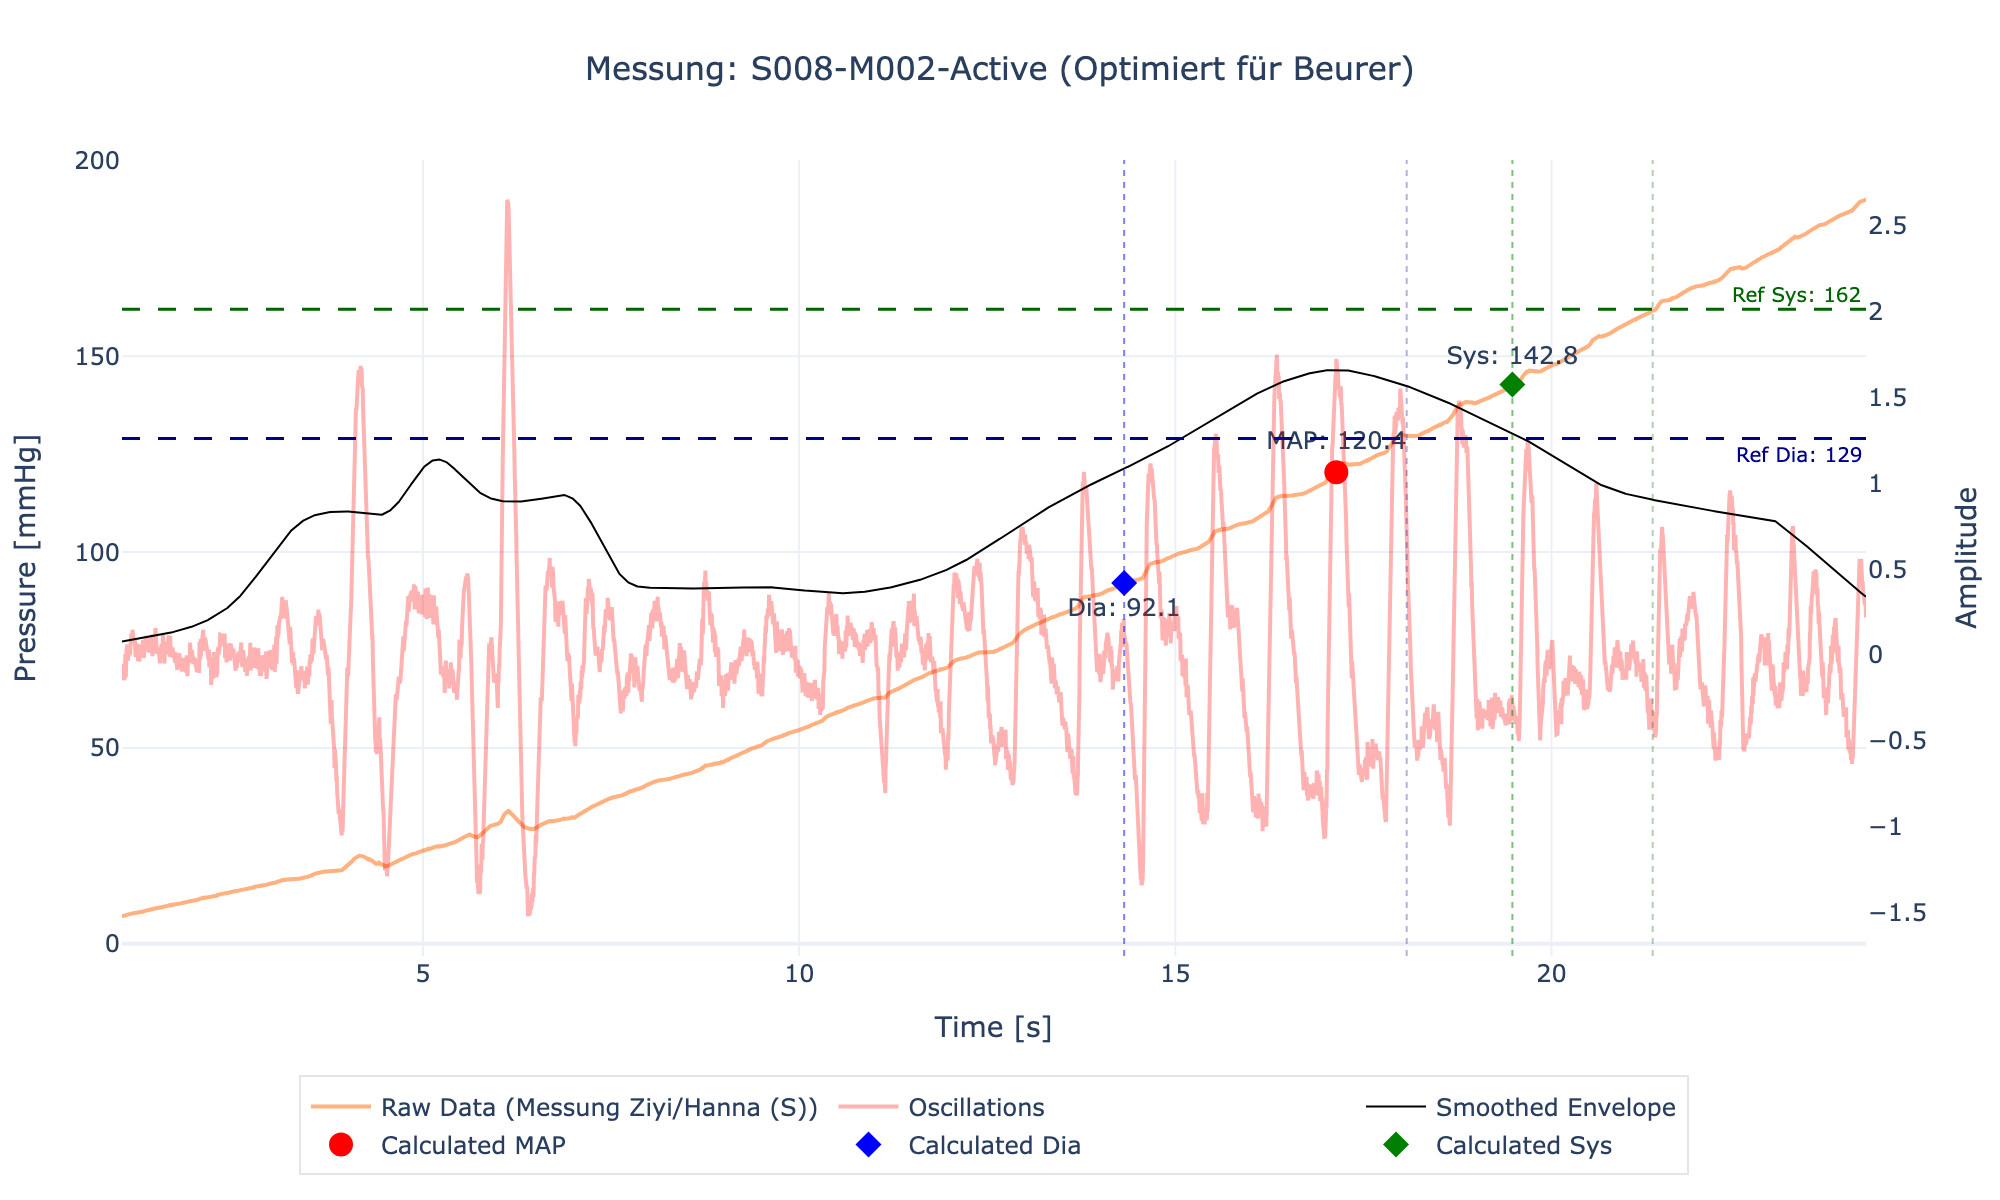
\includegraphics[width=\textwidth]{images/S008-M002-Active_beurer.png}
        \caption{Optimiert für Beurer}
    \end{subfigure}
    \hfill
    \begin{subfigure}[b]{0.48\textwidth}
        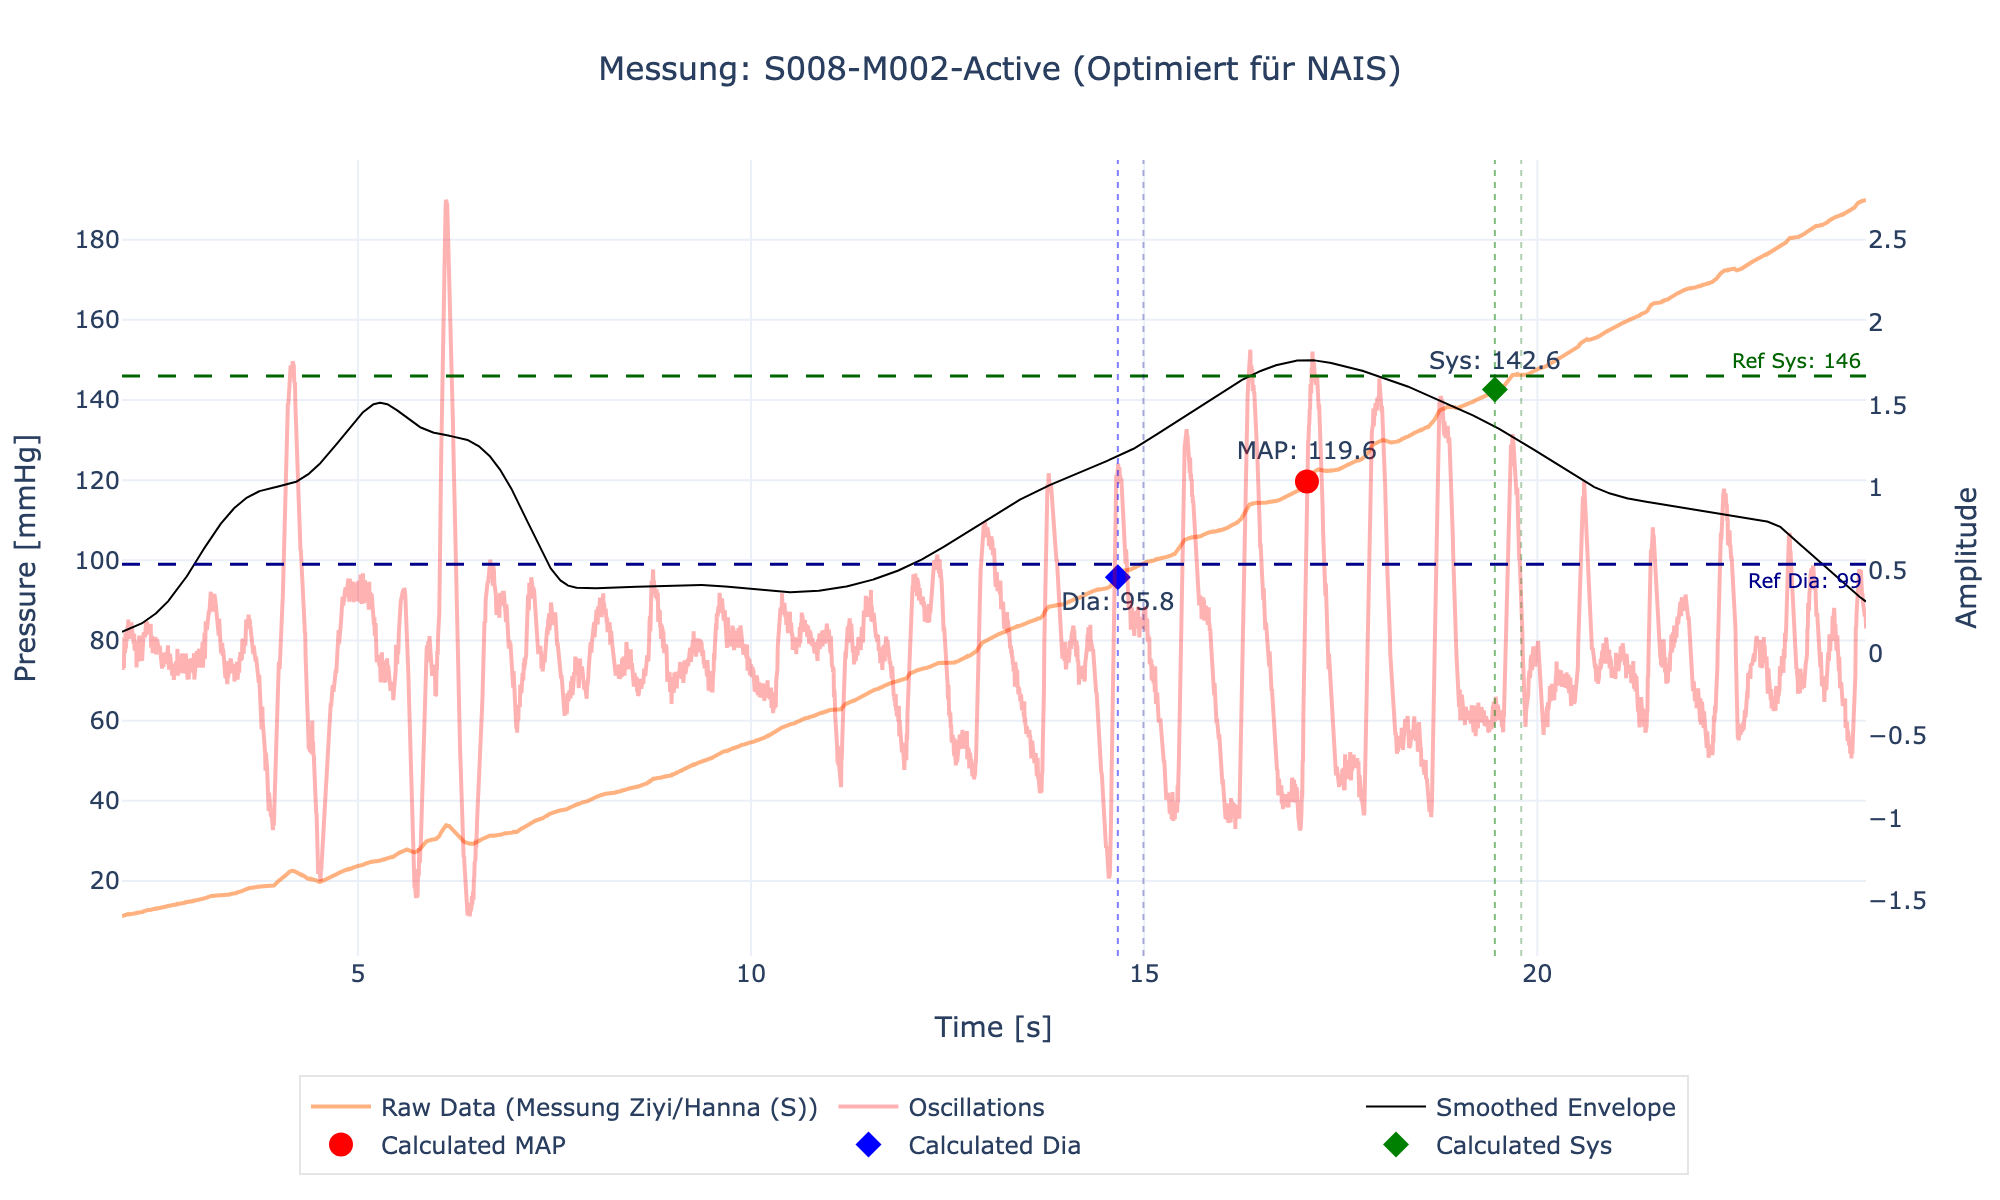
\includegraphics[width=\textwidth]{images/S008-M002-Active_nais.png}
        \caption{Optimiert für NAIS}
    \end{subfigure}
    \caption{Einzelauswertung der Messung S008-M002-Active mit verschiedenen Parametersätzen.}
\end{figure}
\newpage

\subsection*{Messung: S009-M001-Rest}
\begin{figure}[H]
    \centering
    \begin{subfigure}[b]{0.8\textwidth}
        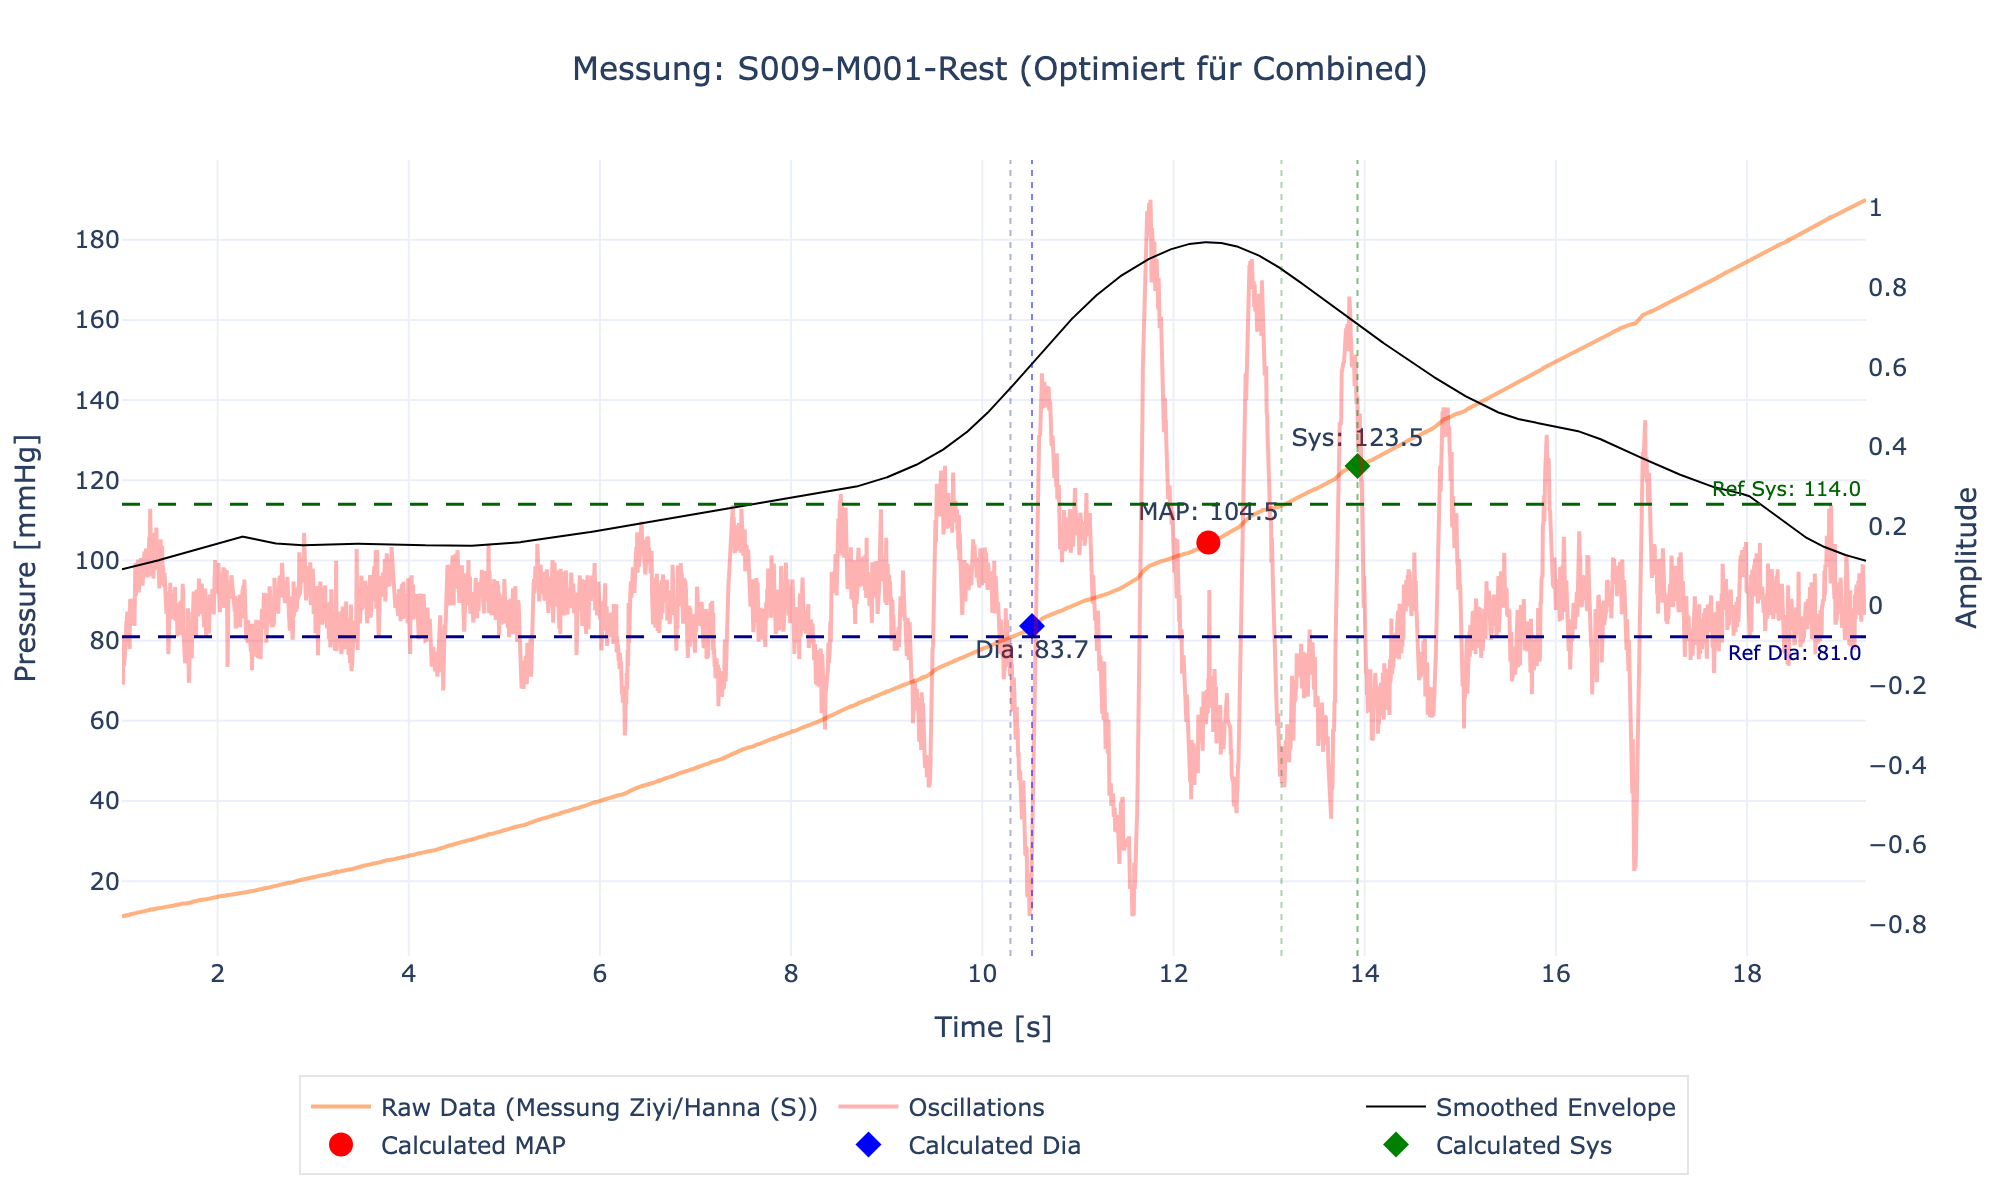
\includegraphics[width=\textwidth]{images/S009-M001-Rest_combined.png}
        \caption{Optimiert für Beurer und NAIS (Kombiniert)}
    \end{subfigure} \\
    \begin{subfigure}[b]{0.48\textwidth}
        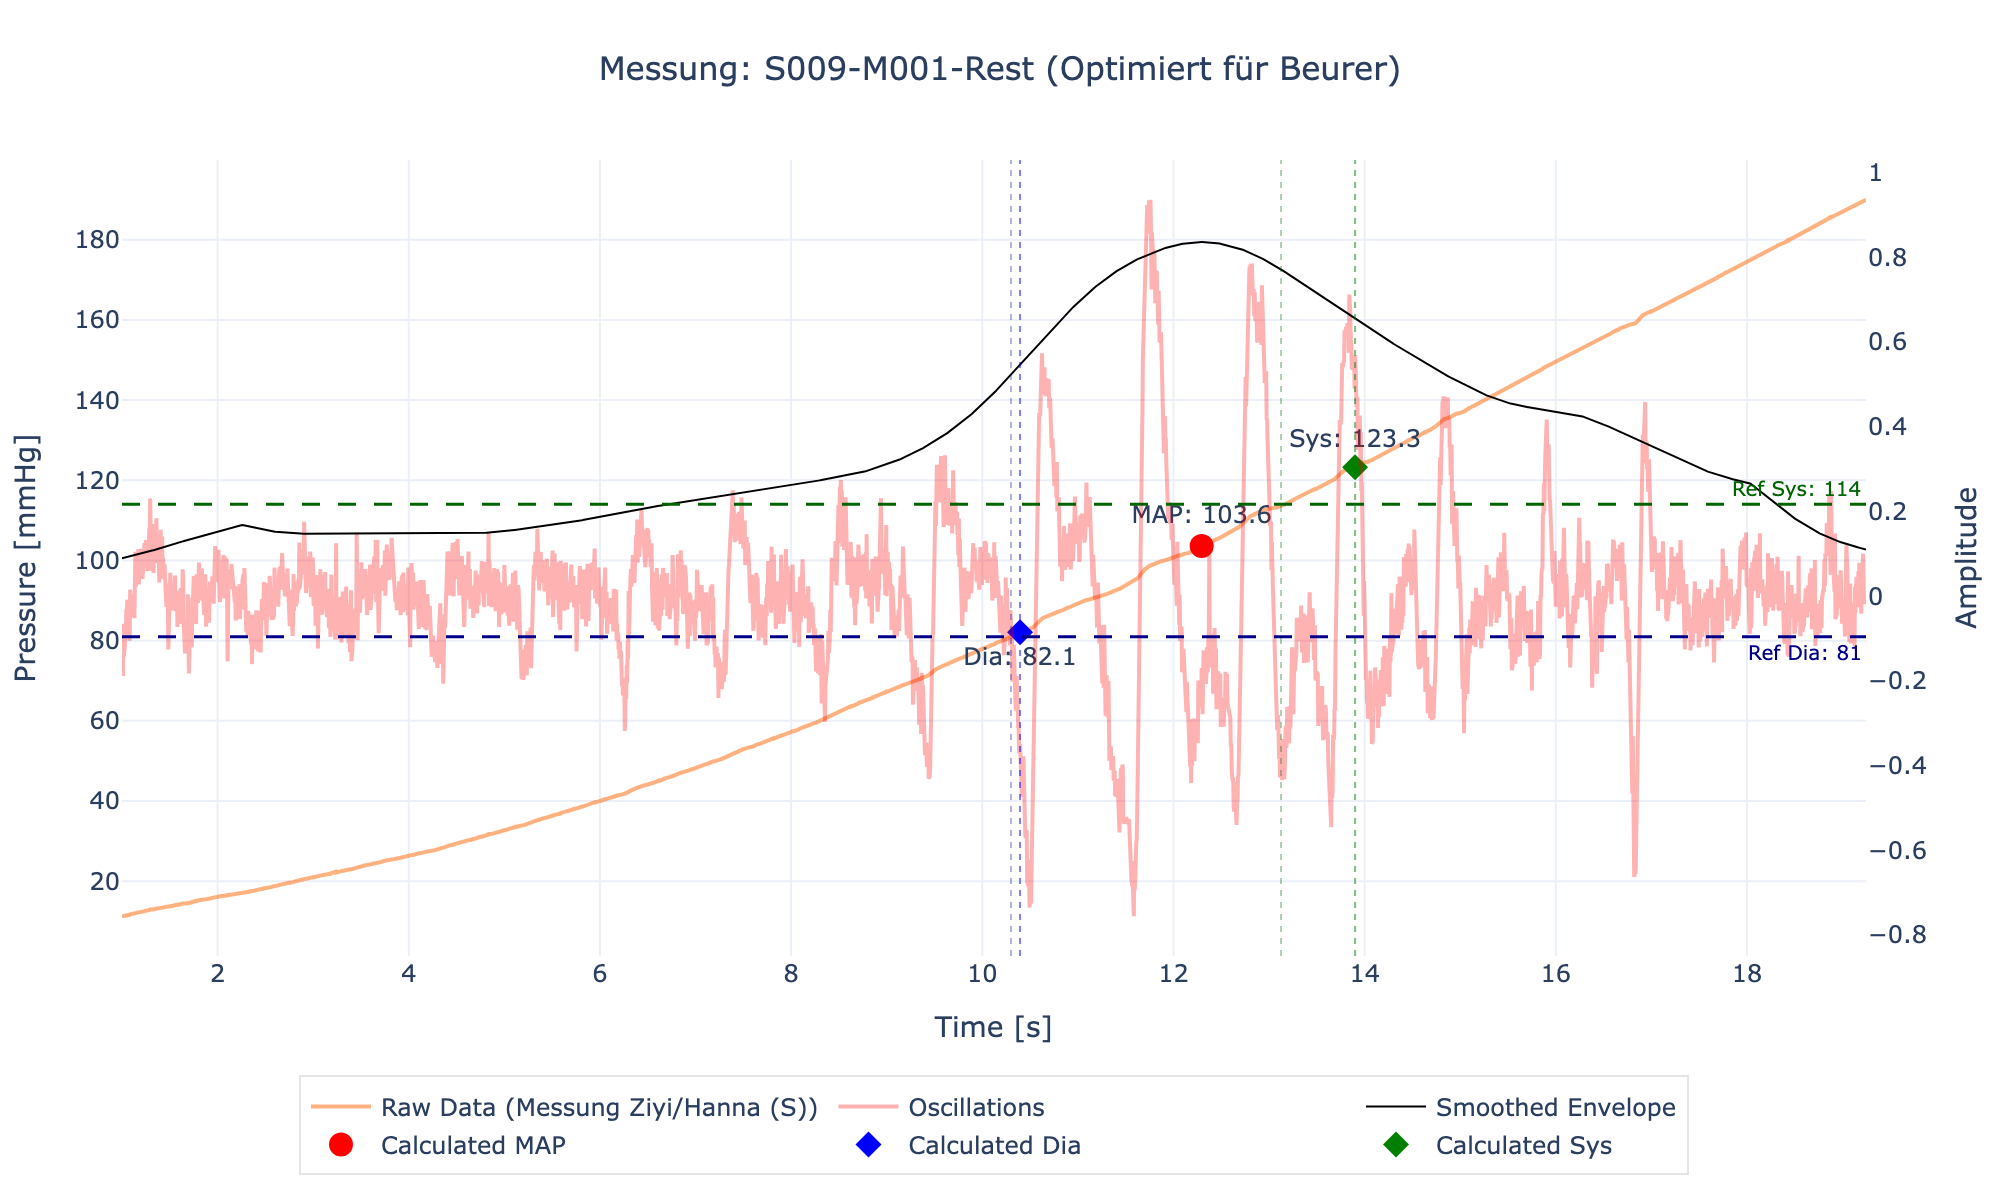
\includegraphics[width=\textwidth]{images/S009-M001-Rest_beurer.png}
        \caption{Optimiert für Beurer}
    \end{subfigure}
    \hfill
    \begin{subfigure}[b]{0.48\textwidth}
        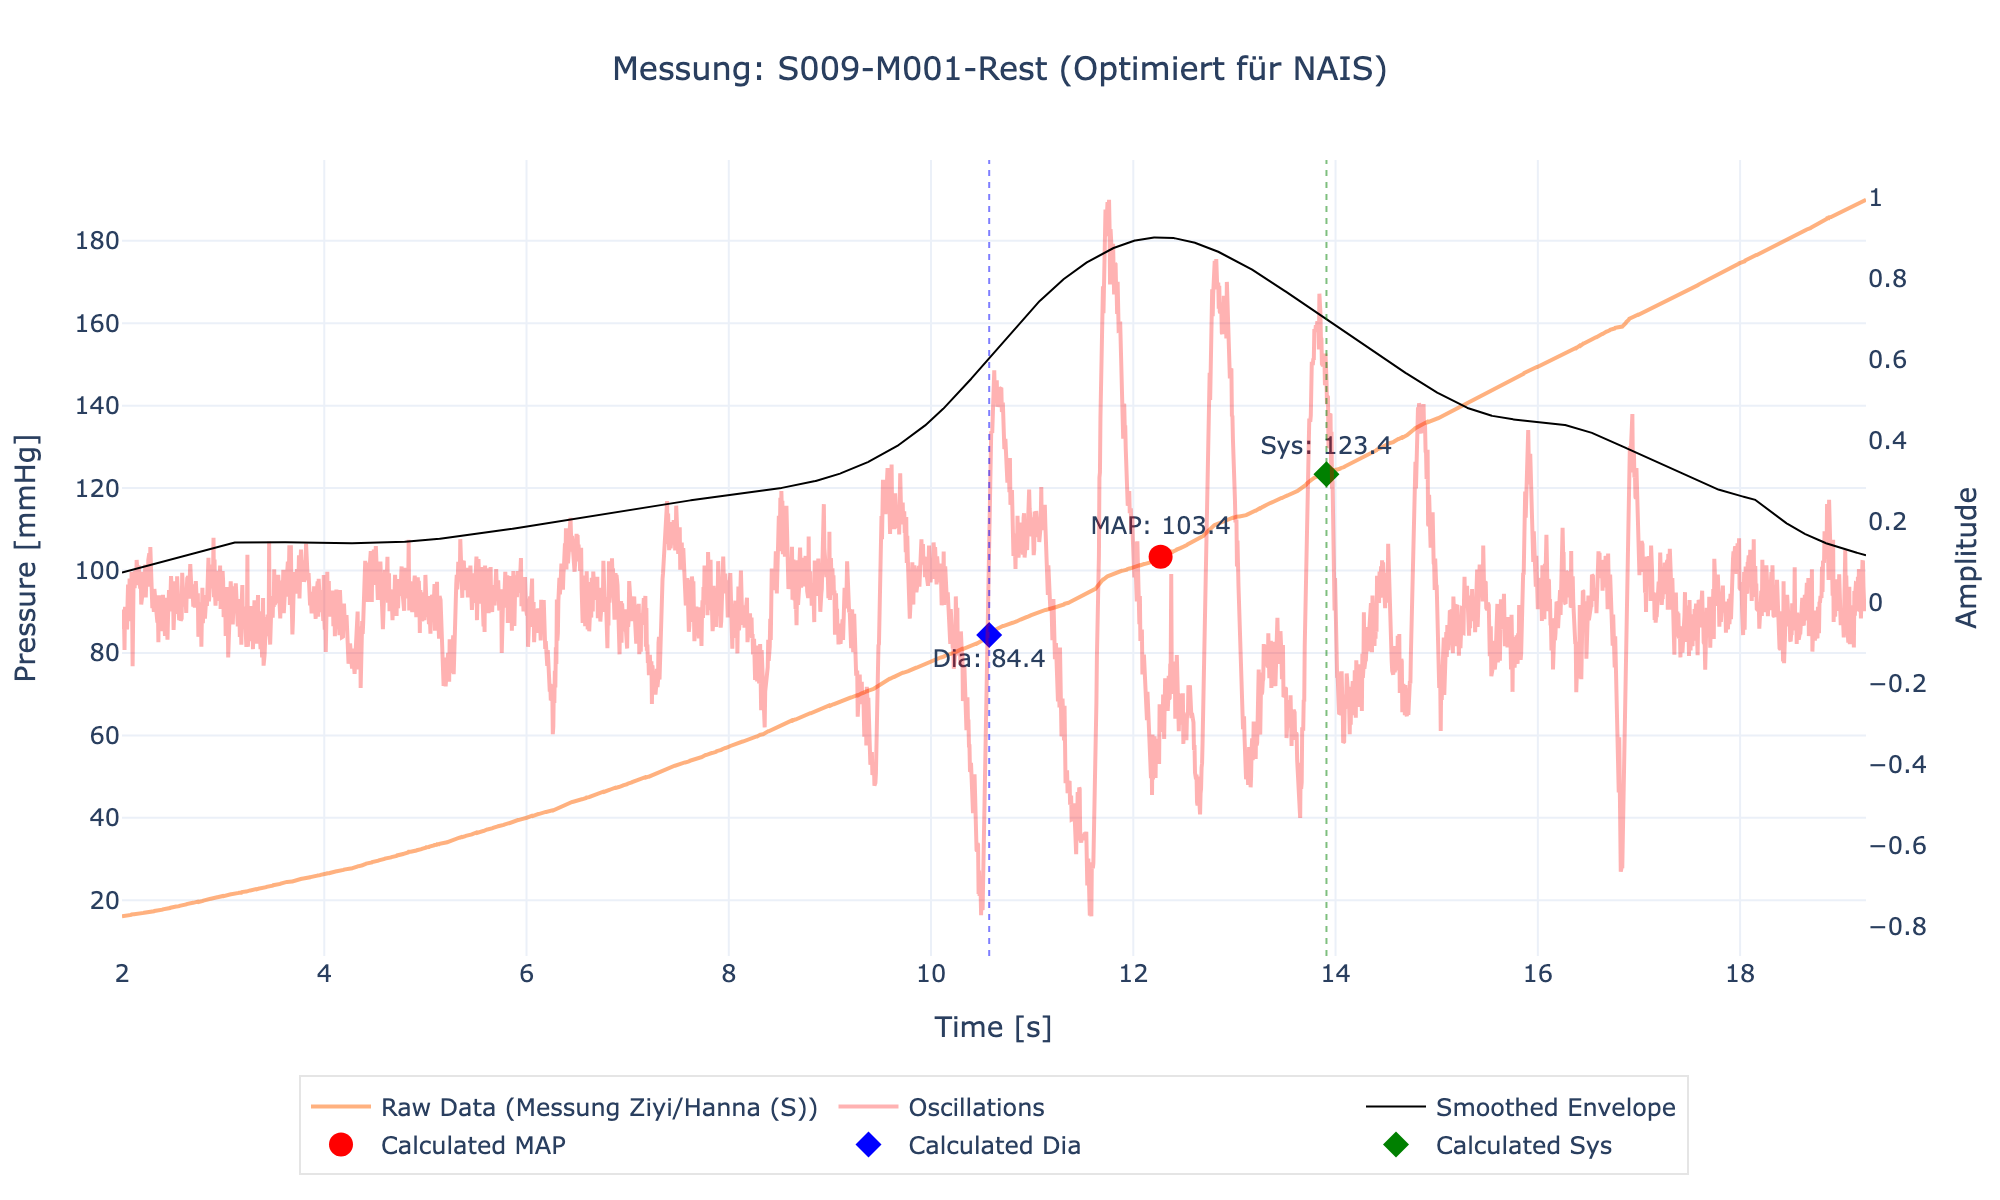
\includegraphics[width=\textwidth]{images/S009-M001-Rest_nais.png}
        \caption{Optimiert für NAIS}
    \end{subfigure}
    \caption{Einzelauswertung der Messung S009-M001-Rest mit verschiedenen Parametersätzen.}
\end{figure}
\newpage

\subsection*{Messung: S009-M002-Active}
\begin{figure}[H]
    \centering
    \begin{subfigure}[b]{0.8\textwidth}
        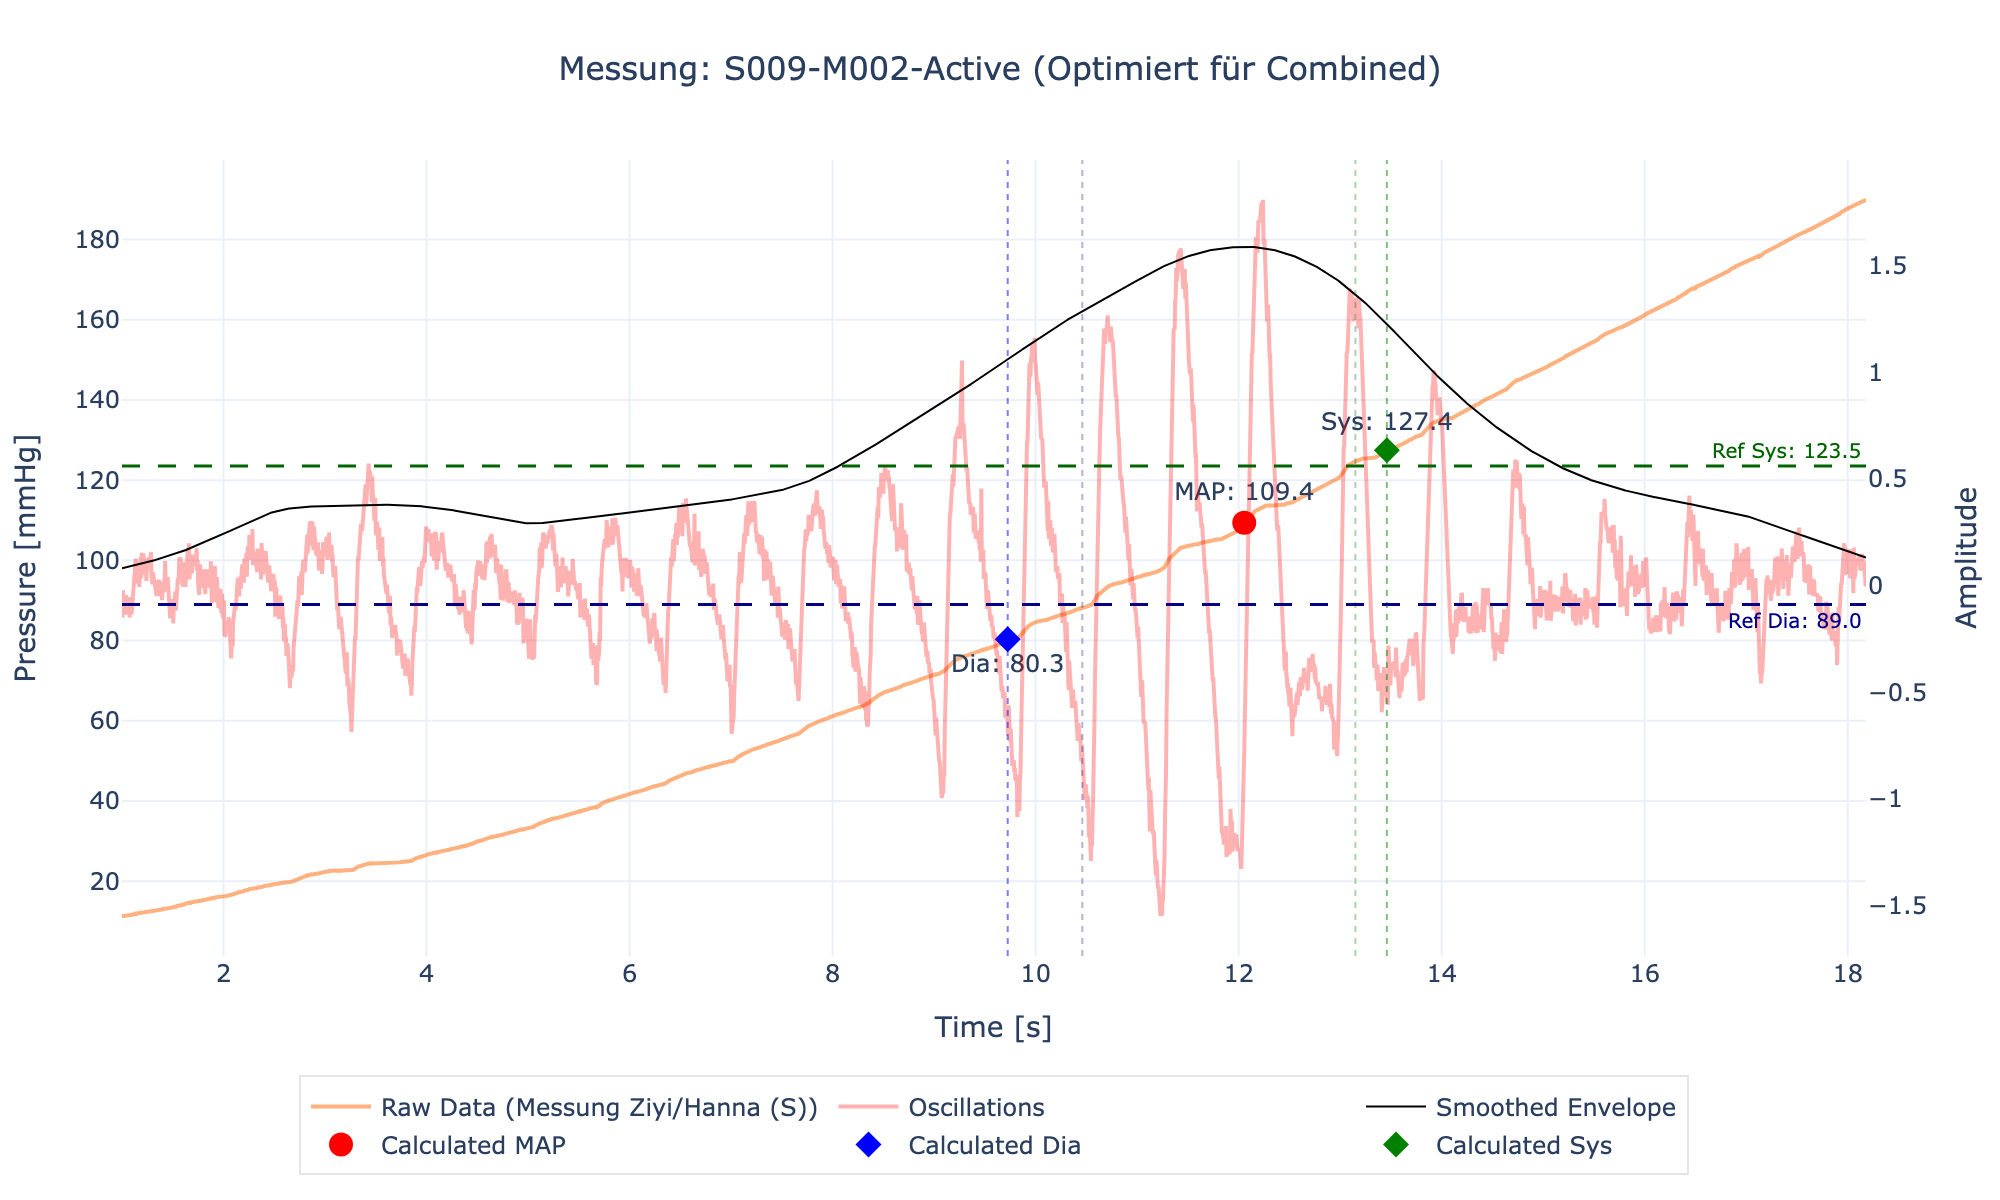
\includegraphics[width=\textwidth]{images/S009-M002-Active_combined.png}
        \caption{Optimiert für Beurer und NAIS (Kombiniert)}
    \end{subfigure} \\
    \begin{subfigure}[b]{0.48\textwidth}
        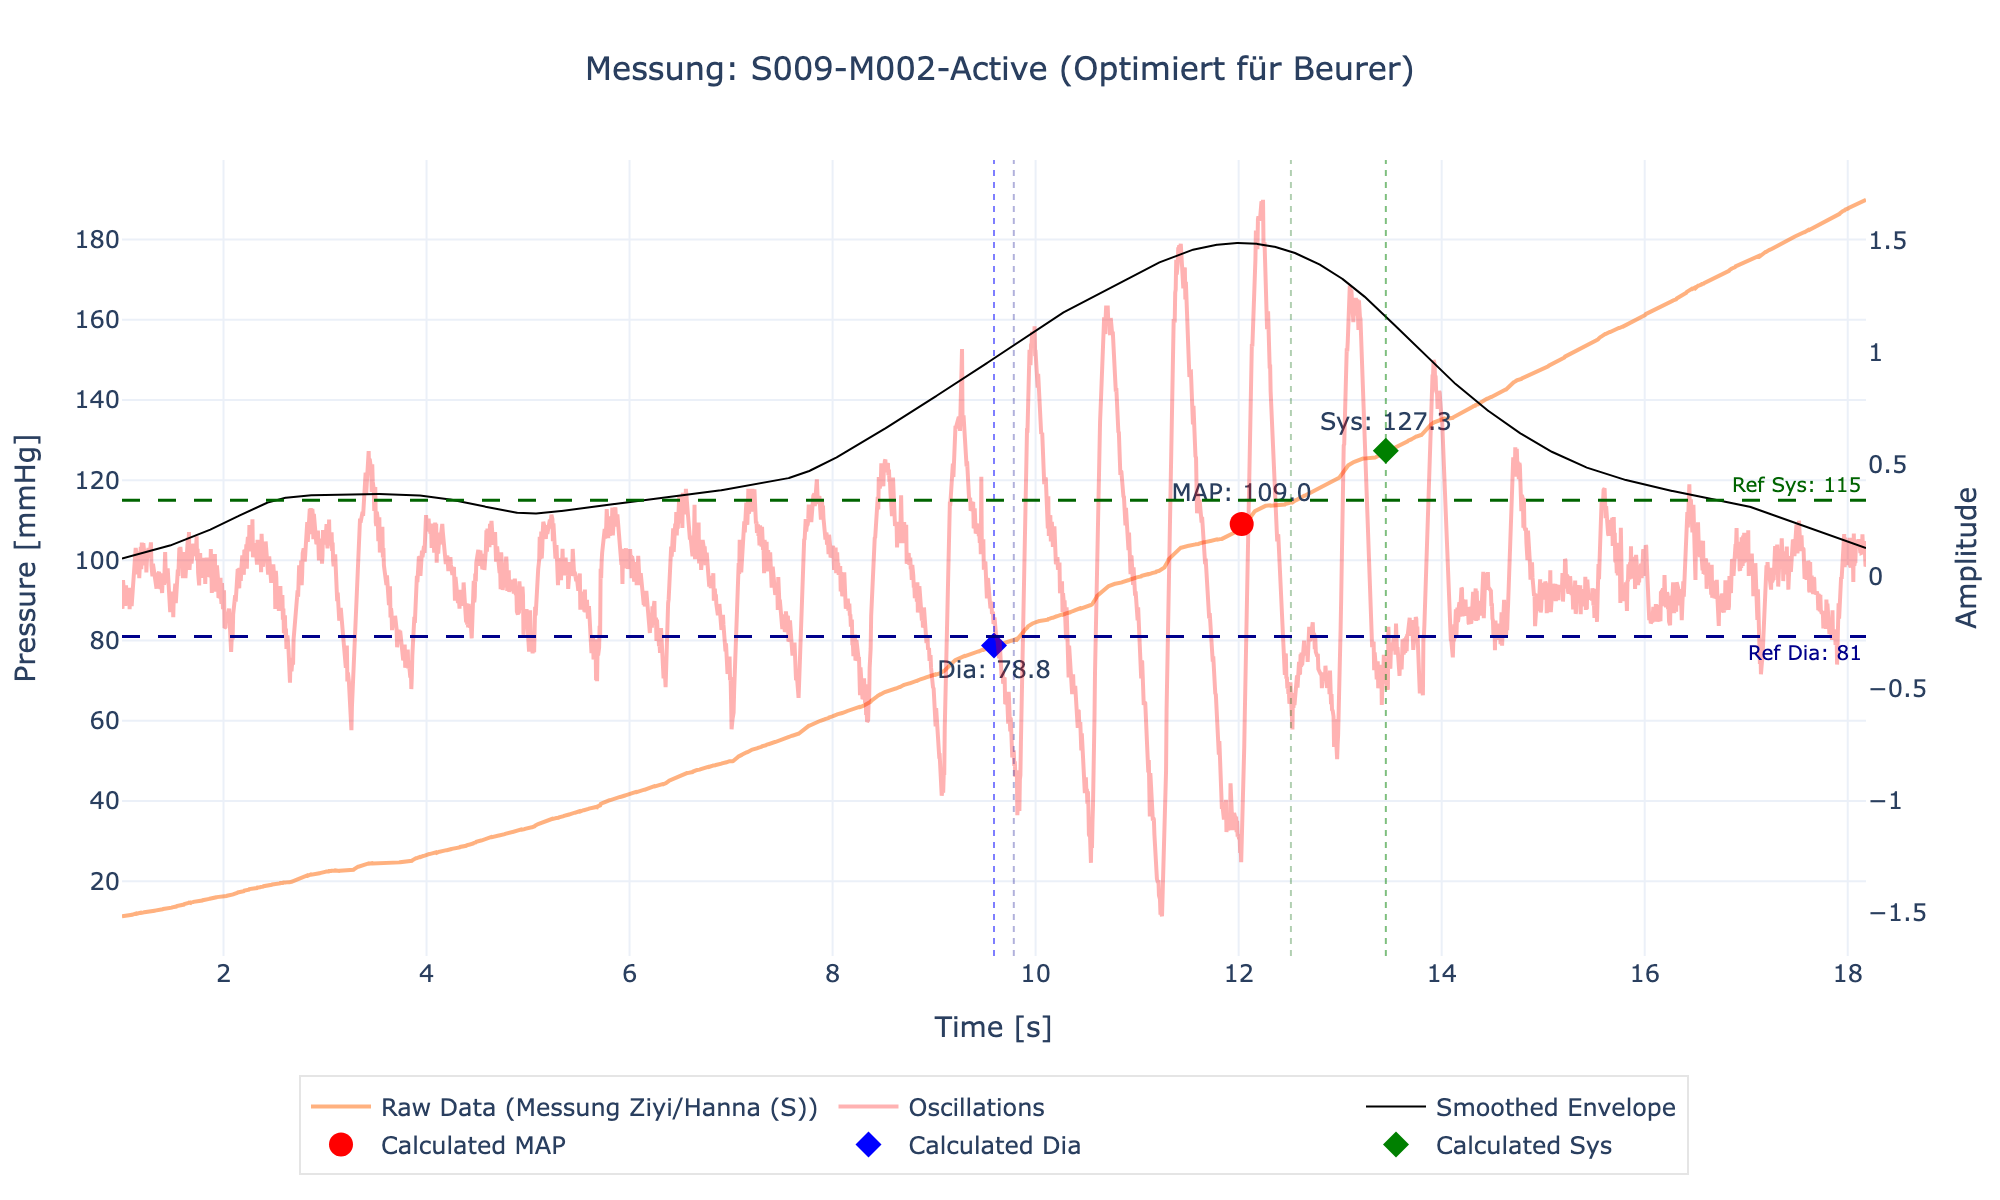
\includegraphics[width=\textwidth]{images/S009-M002-Active_beurer.png}
        \caption{Optimiert für Beurer}
    \end{subfigure}
    \hfill
    \begin{subfigure}[b]{0.48\textwidth}
        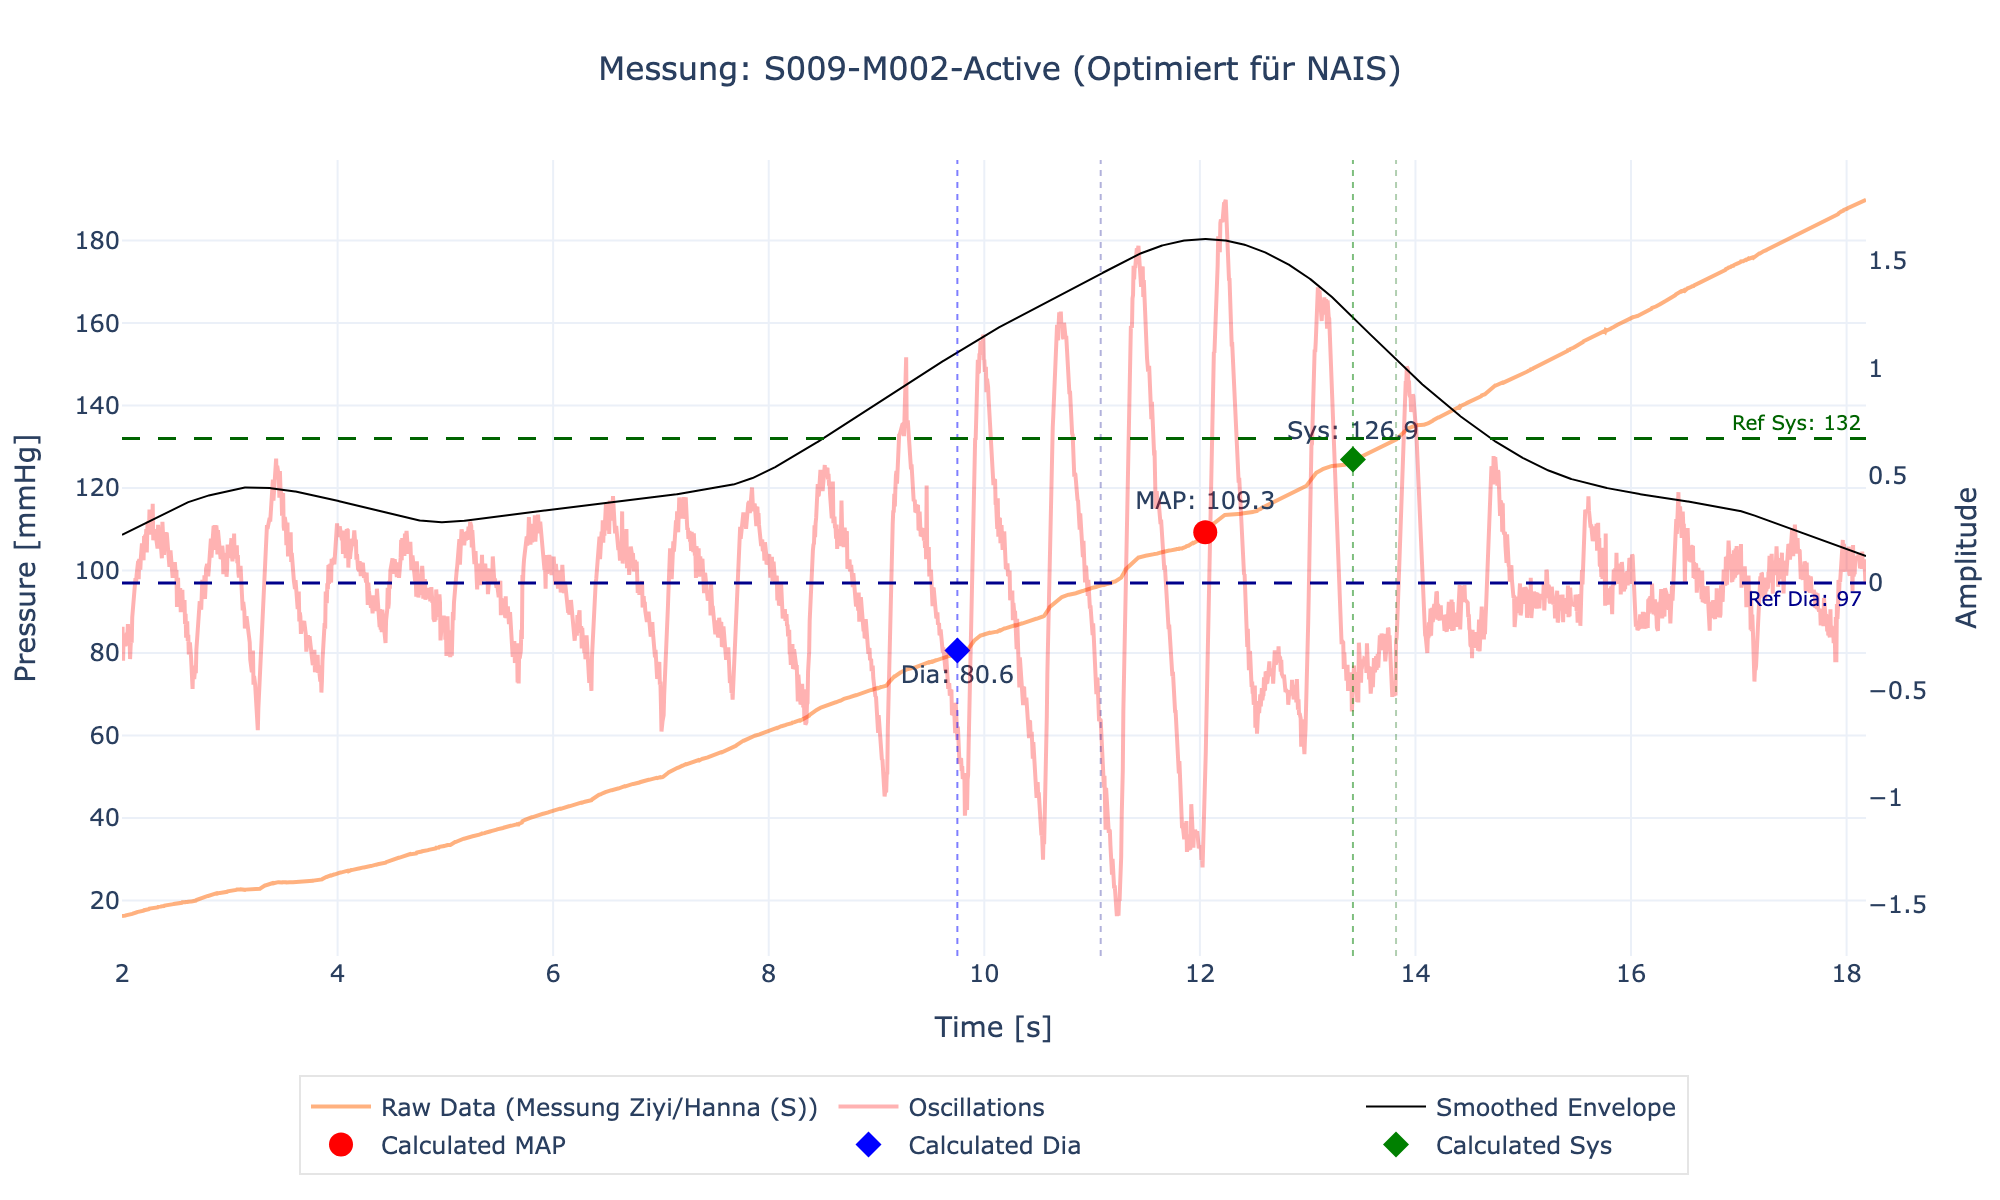
\includegraphics[width=\textwidth]{images/S009-M002-Active_nais.png}
        \caption{Optimiert für NAIS}
    \end{subfigure}
    \caption{Einzelauswertung der Messung S009-M002-Active mit verschiedenen Parametersätzen.}
\end{figure}
\newpage

\subsection*{Messung: S010-M001-Rest}
\begin{figure}[H]
    \centering
    \begin{subfigure}[b]{0.8\textwidth}
        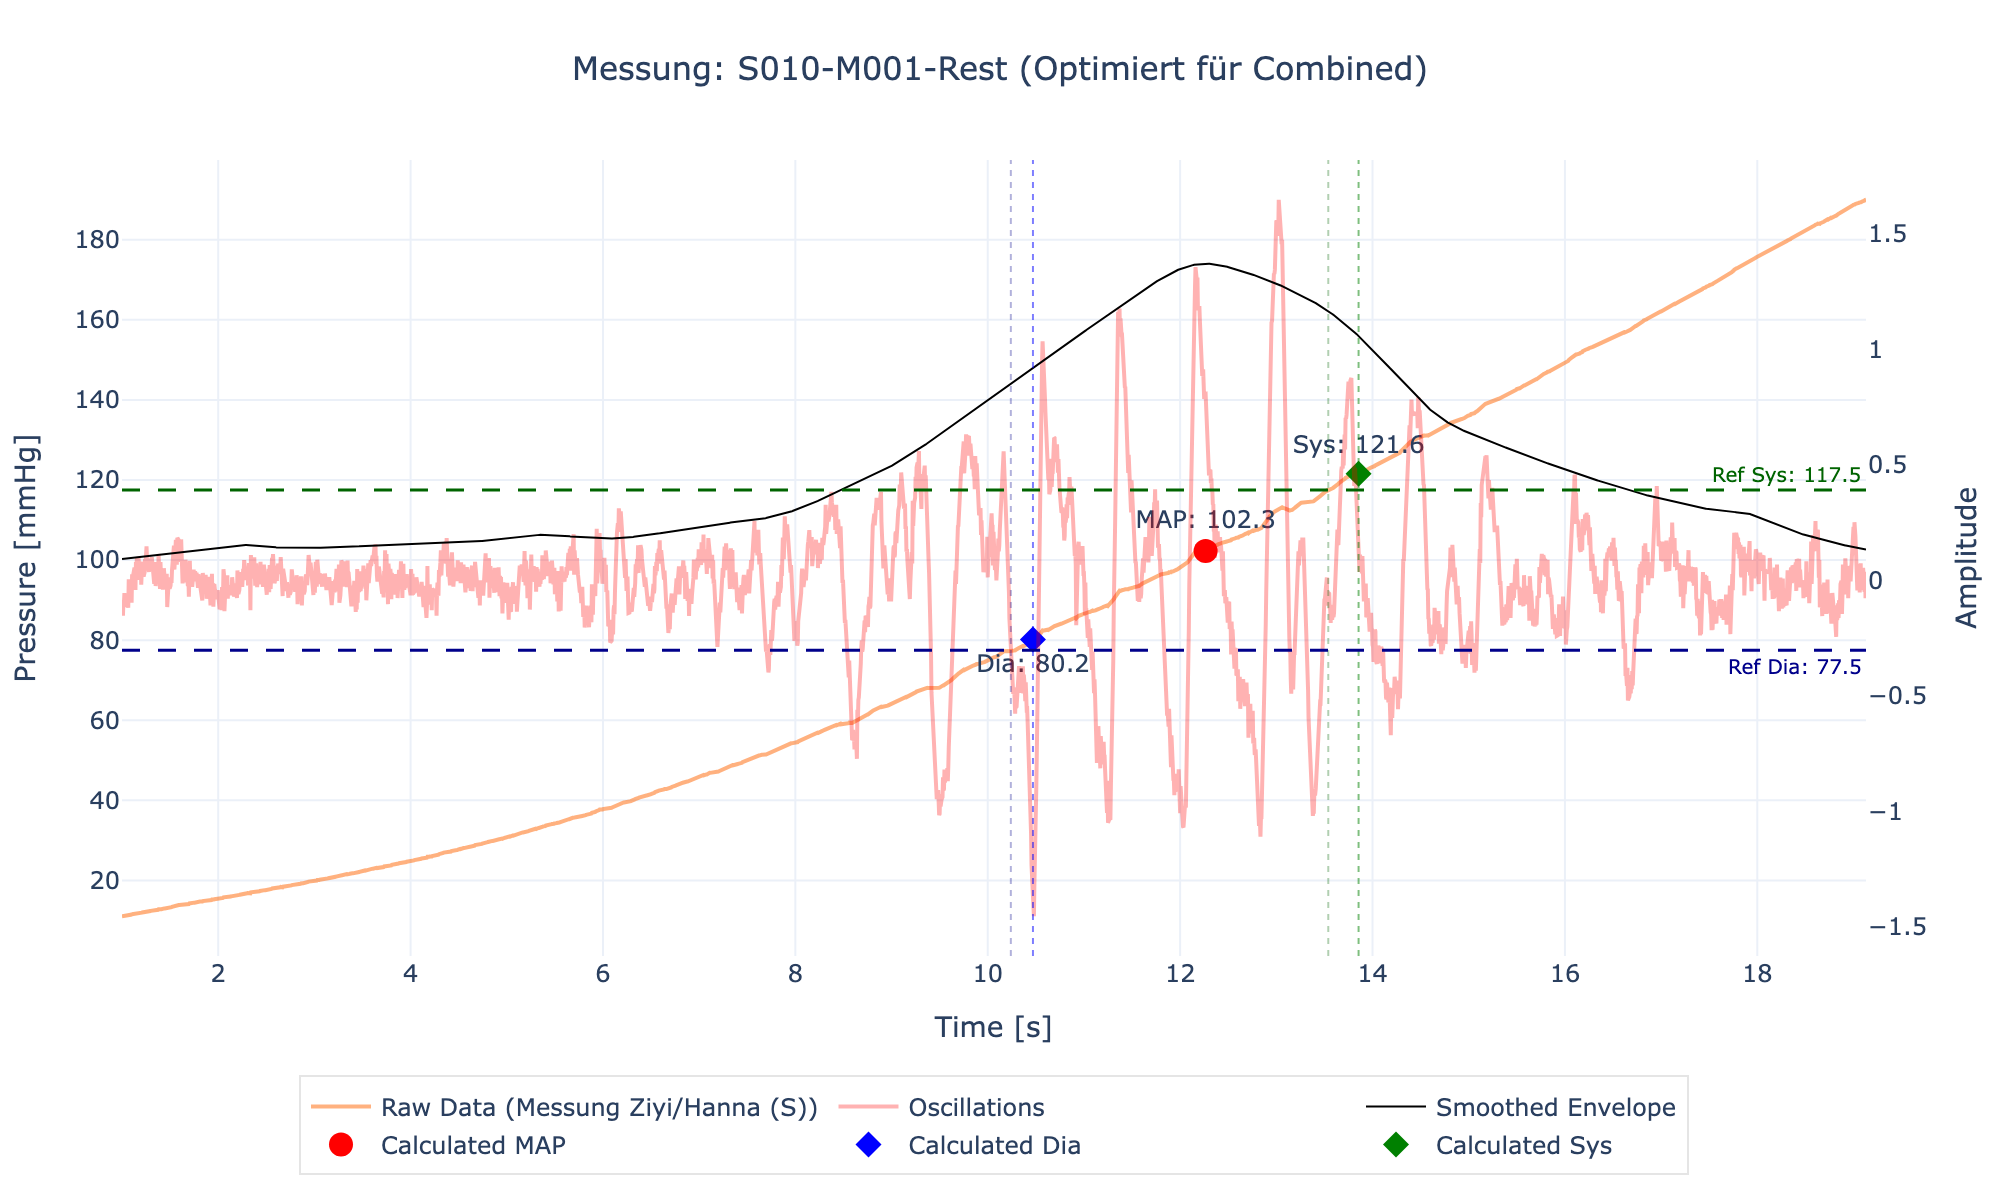
\includegraphics[width=\textwidth]{images/S010-M001-Rest_combined.png}
        \caption{Optimiert für Beurer und NAIS (Kombiniert)}
    \end{subfigure} \\
    \begin{subfigure}[b]{0.48\textwidth}
        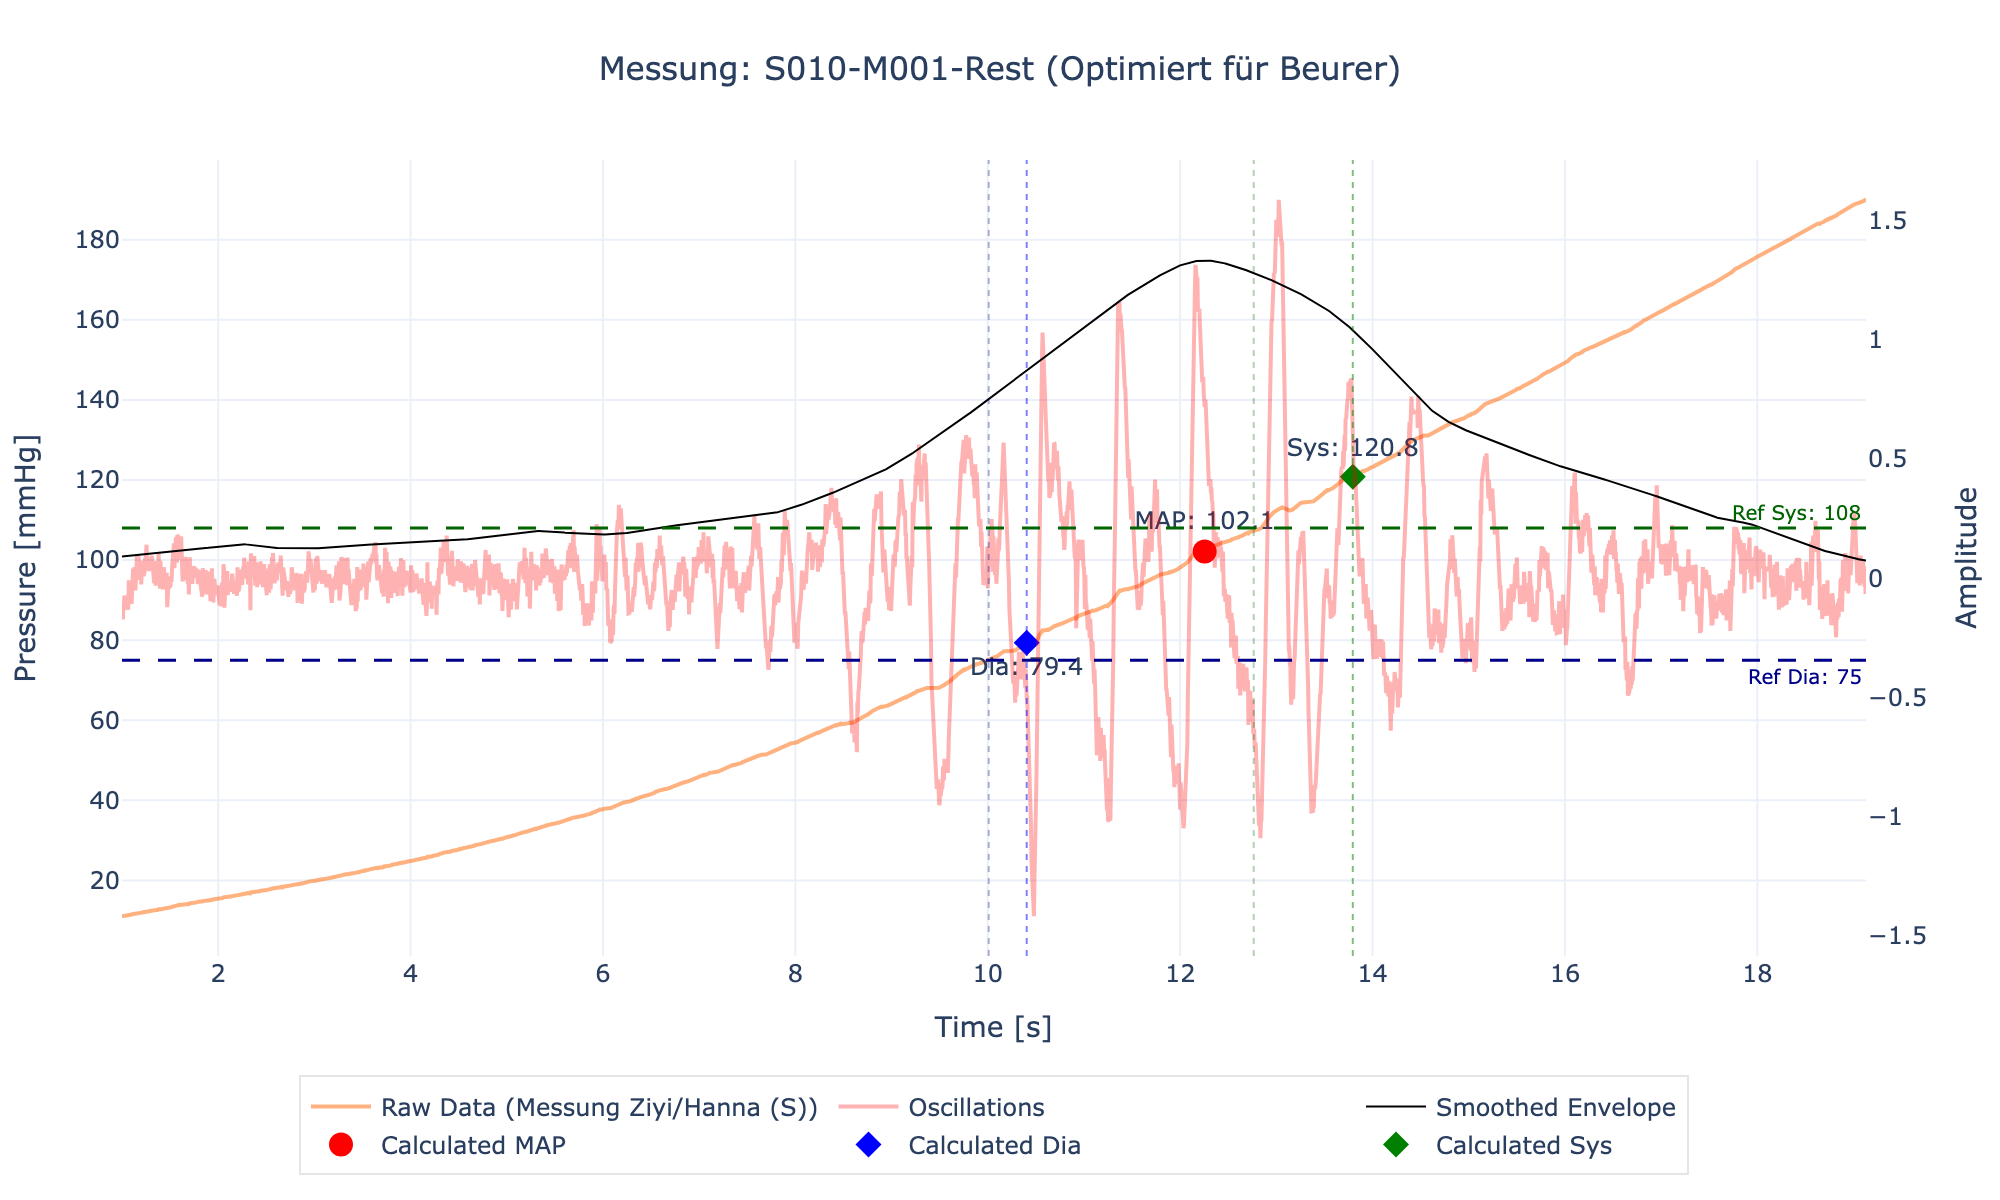
\includegraphics[width=\textwidth]{images/S010-M001-Rest_beurer.png}
        \caption{Optimiert für Beurer}
    \end{subfigure}
    \hfill
    \begin{subfigure}[b]{0.48\textwidth}
        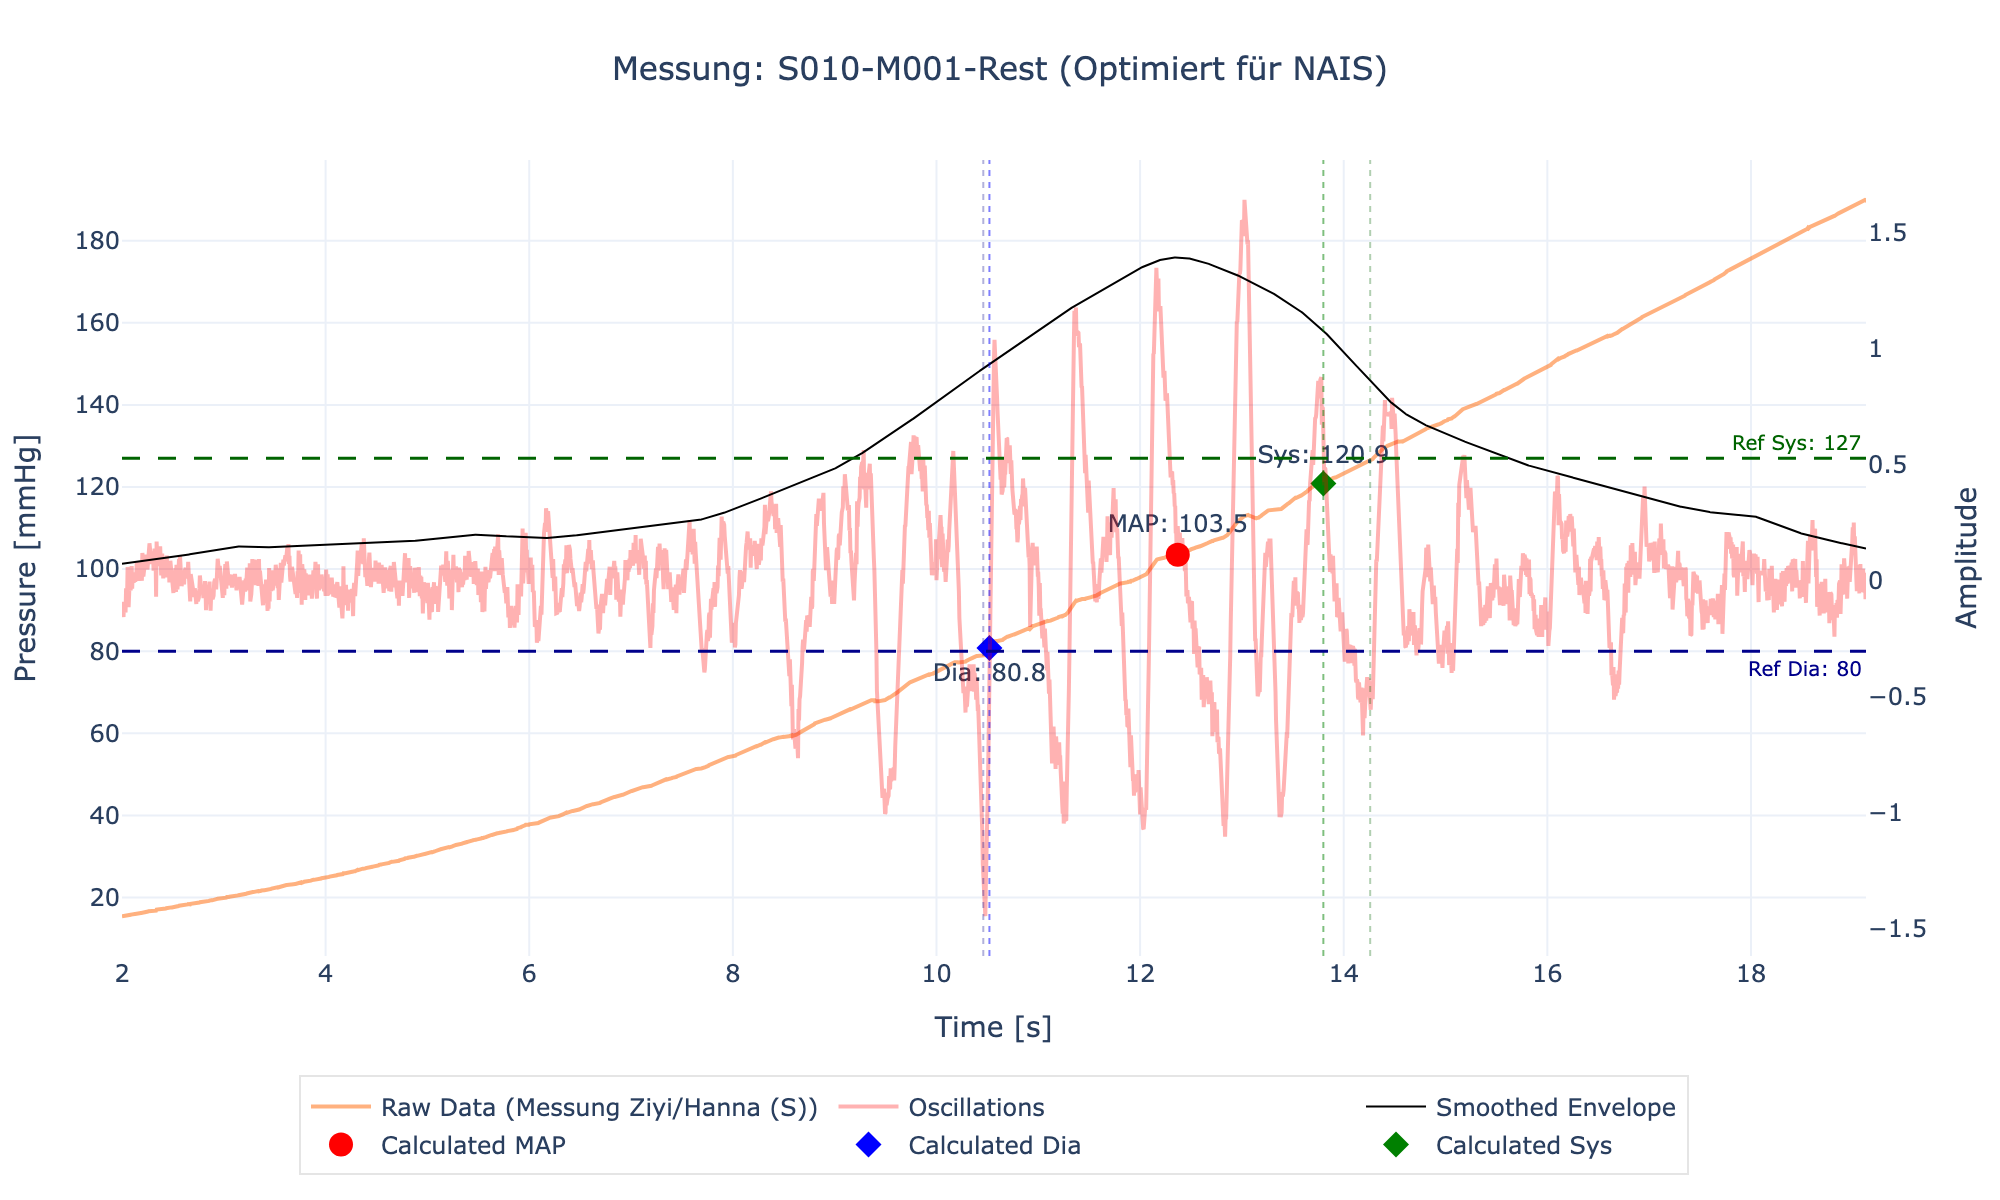
\includegraphics[width=\textwidth]{images/S010-M001-Rest_nais.png}
        \caption{Optimiert für NAIS}
    \end{subfigure}
    \caption{Einzelauswertung der Messung S010-M001-Rest mit verschiedenen Parametersätzen.}
\end{figure}
\newpage

\subsection*{Messung: S010-M002-Active}
\begin{figure}[H]
    \centering
    \begin{subfigure}[b]{0.8\textwidth}
        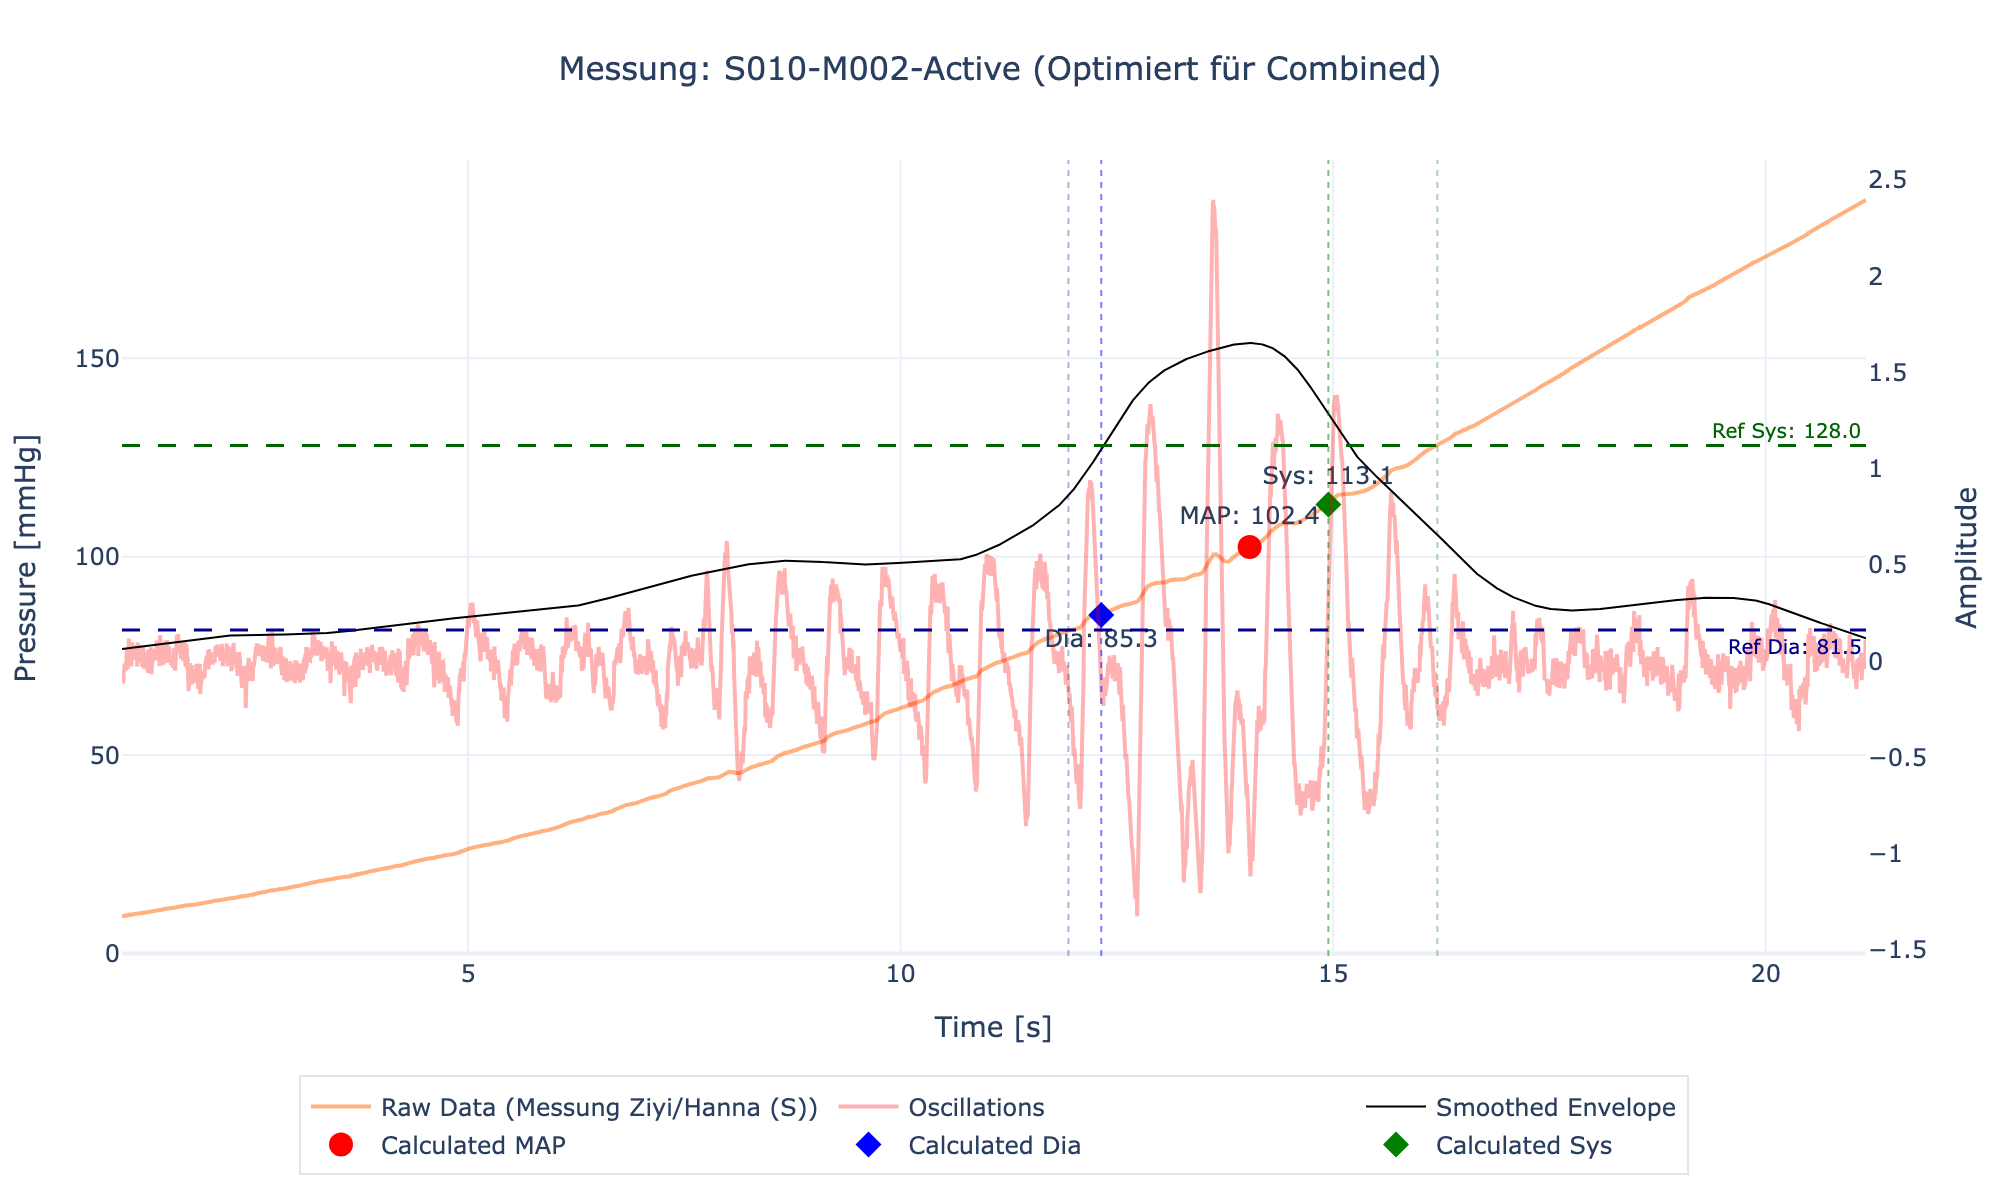
\includegraphics[width=\textwidth]{images/S010-M002-Active_combined.png}
        \caption{Optimiert für Beurer und NAIS (Kombiniert)}
    \end{subfigure} \\
    \begin{subfigure}[b]{0.48\textwidth}
        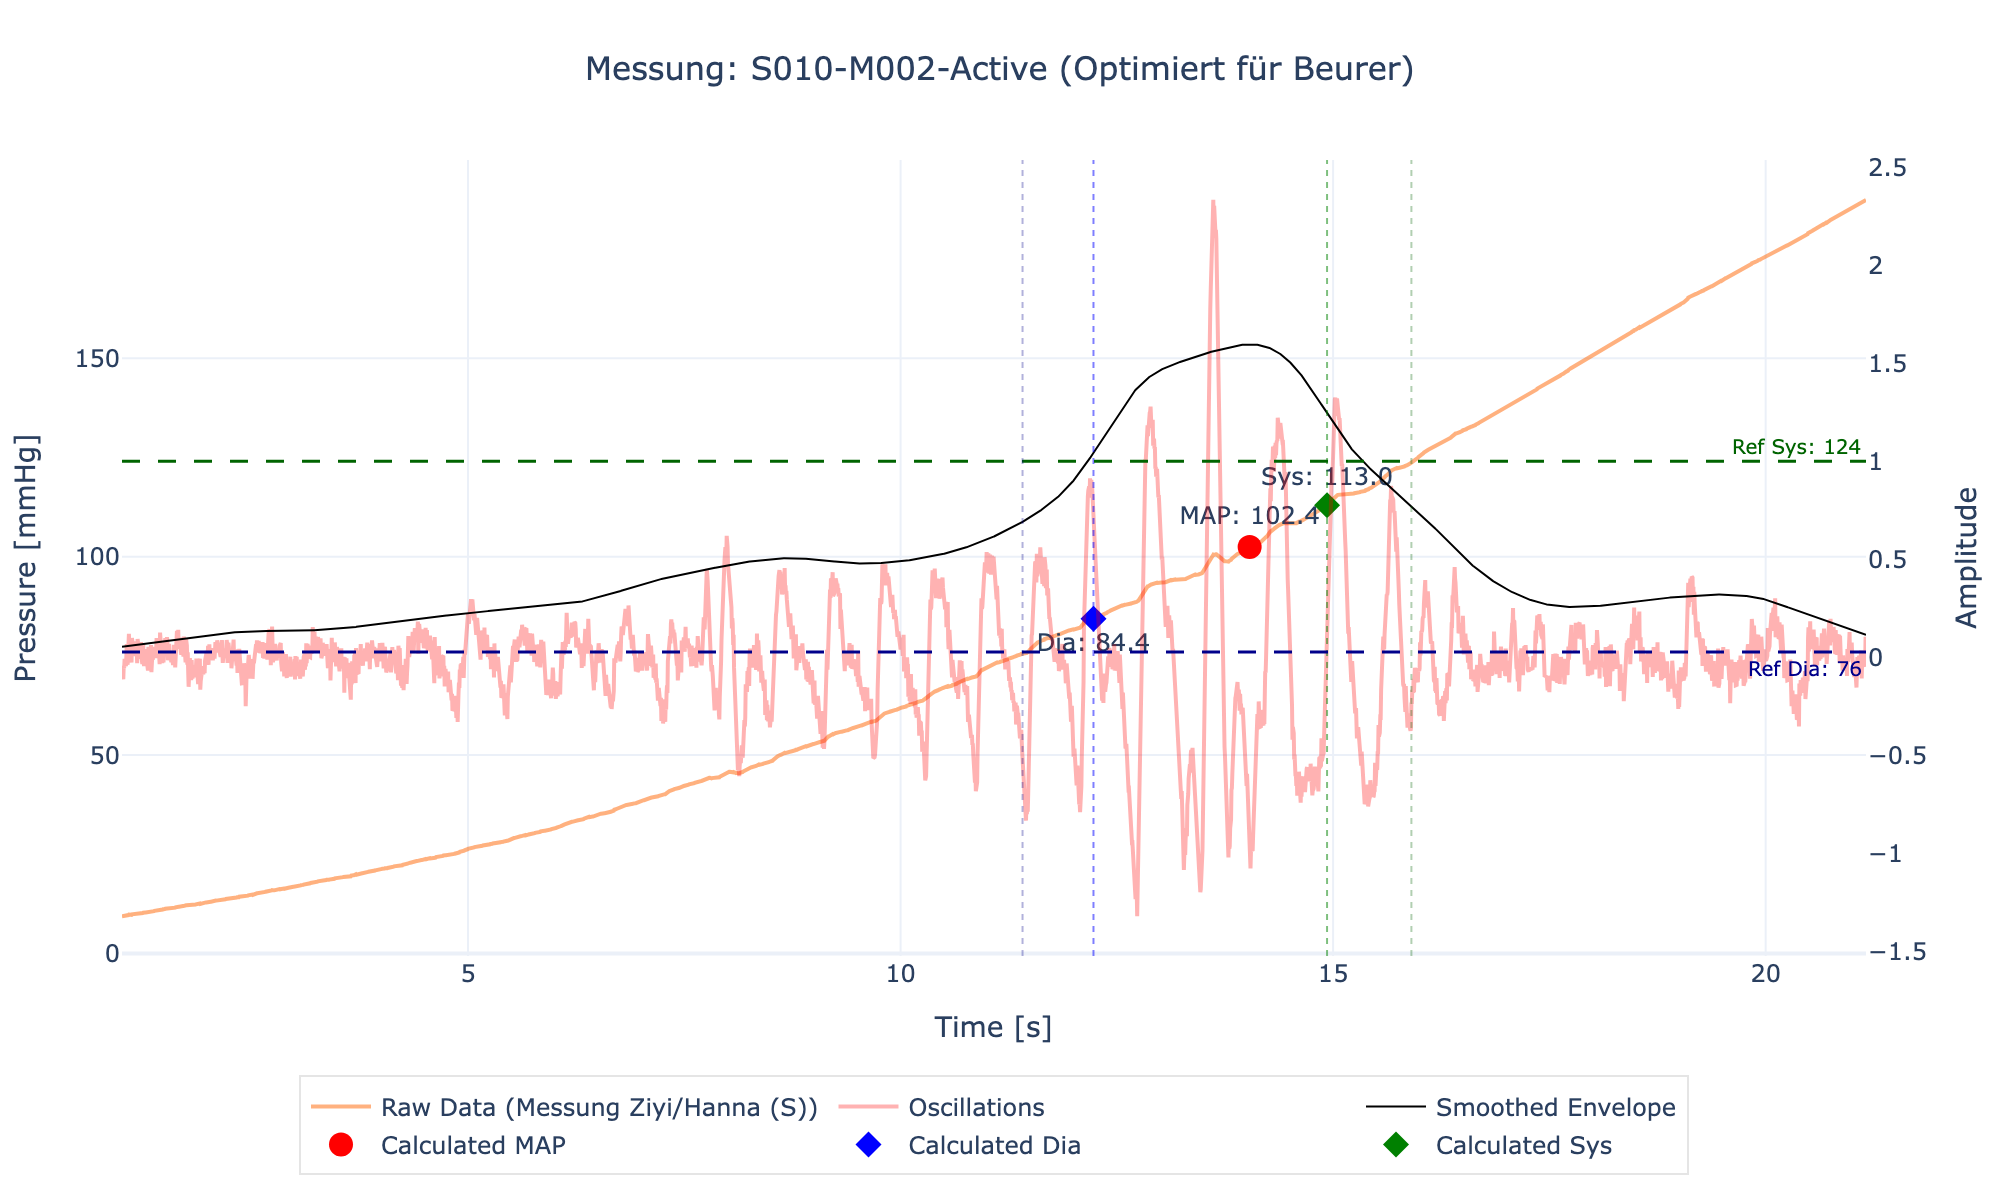
\includegraphics[width=\textwidth]{images/S010-M002-Active_beurer.png}
        \caption{Optimiert für Beurer}
    \end{subfigure}
    \hfill
    \begin{subfigure}[b]{0.48\textwidth}
        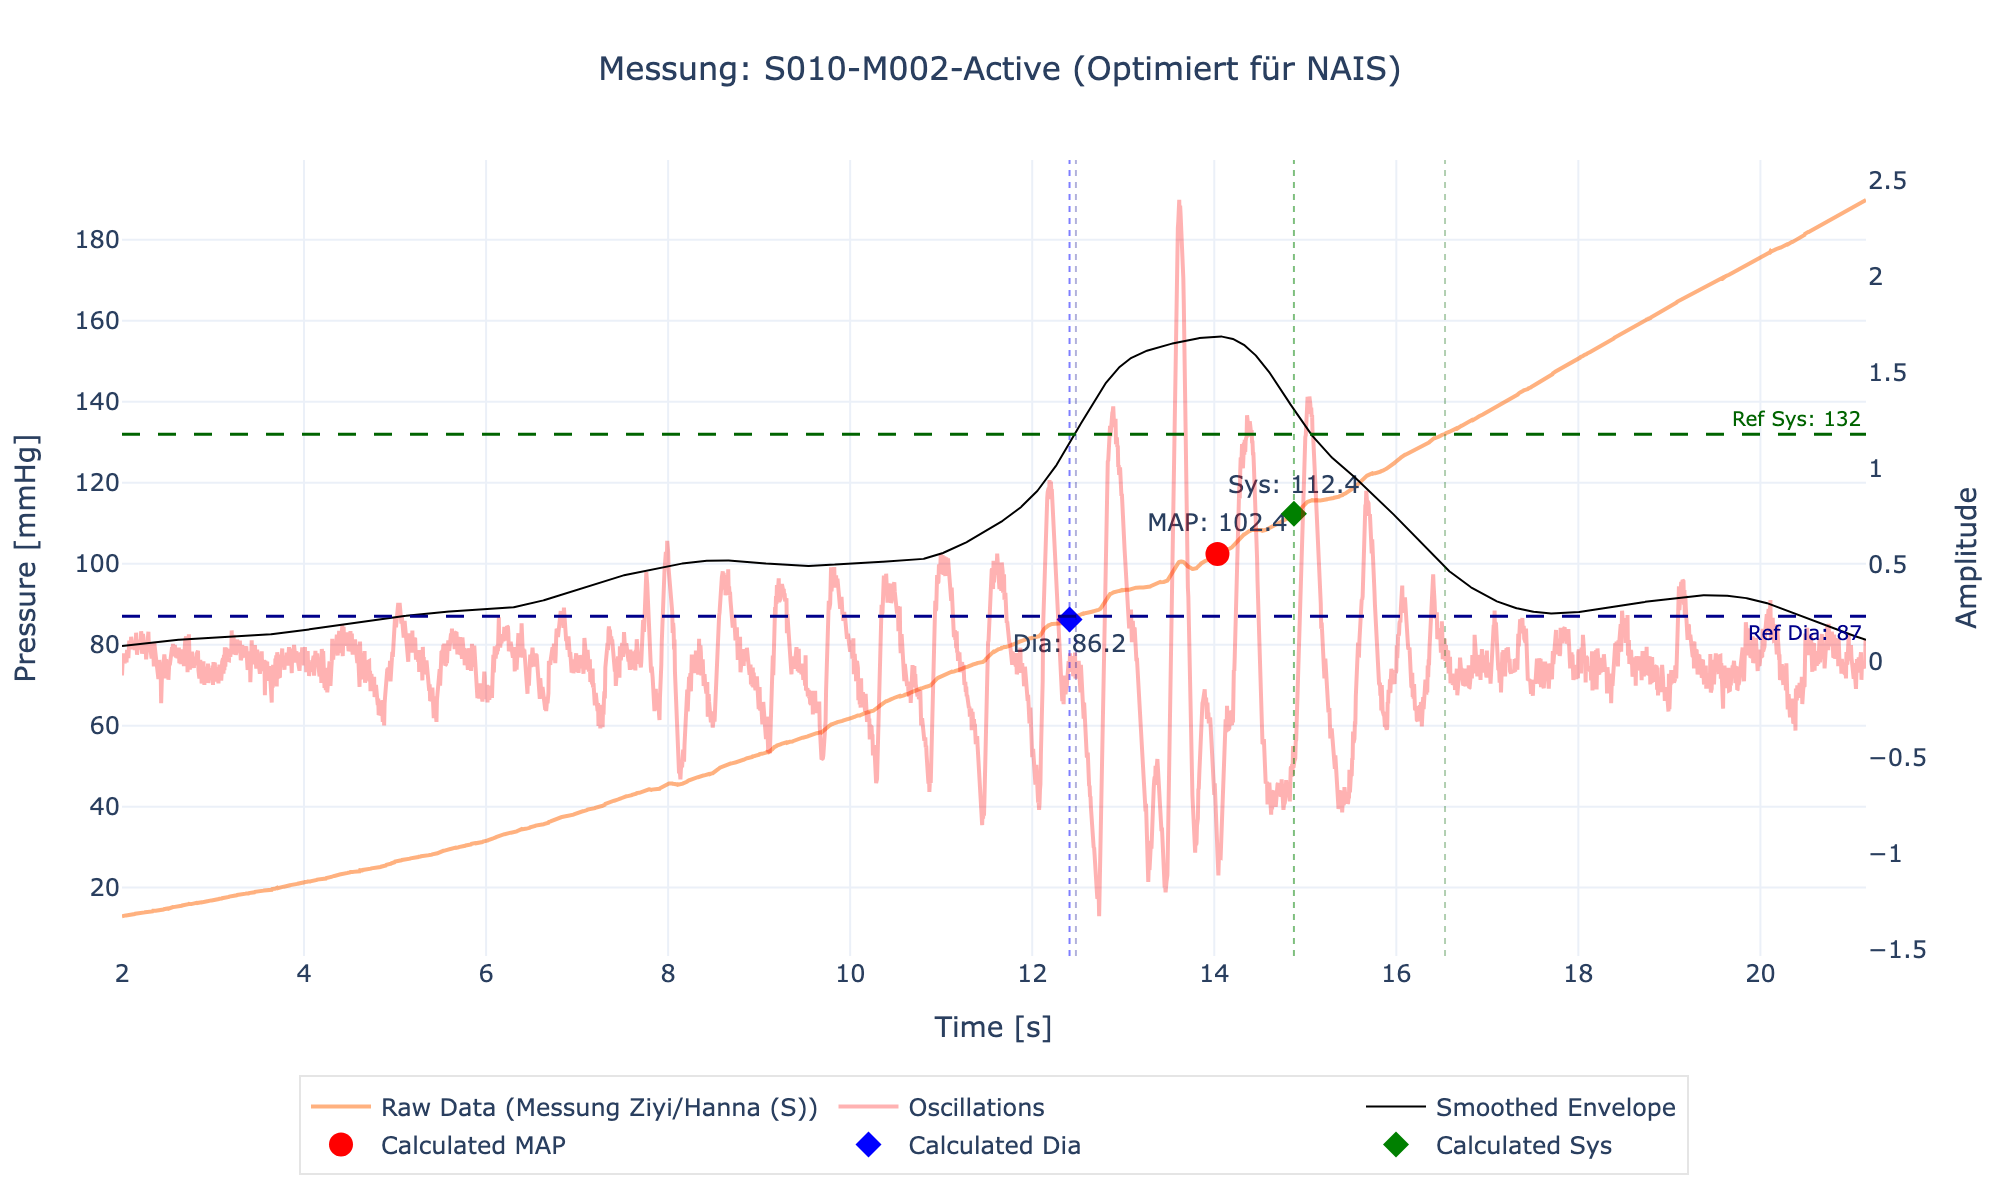
\includegraphics[width=\textwidth]{images/S010-M002-Active_nais.png}
        \caption{Optimiert für NAIS}
    \end{subfigure}
    \caption{Einzelauswertung der Messung S010-M002-Active mit verschiedenen Parametersätzen.}
\end{figure}
\newpage

\subsection*{Messung: S011-M001-Rest}
\begin{figure}[H]
    \centering
    \begin{subfigure}[b]{0.8\textwidth}
        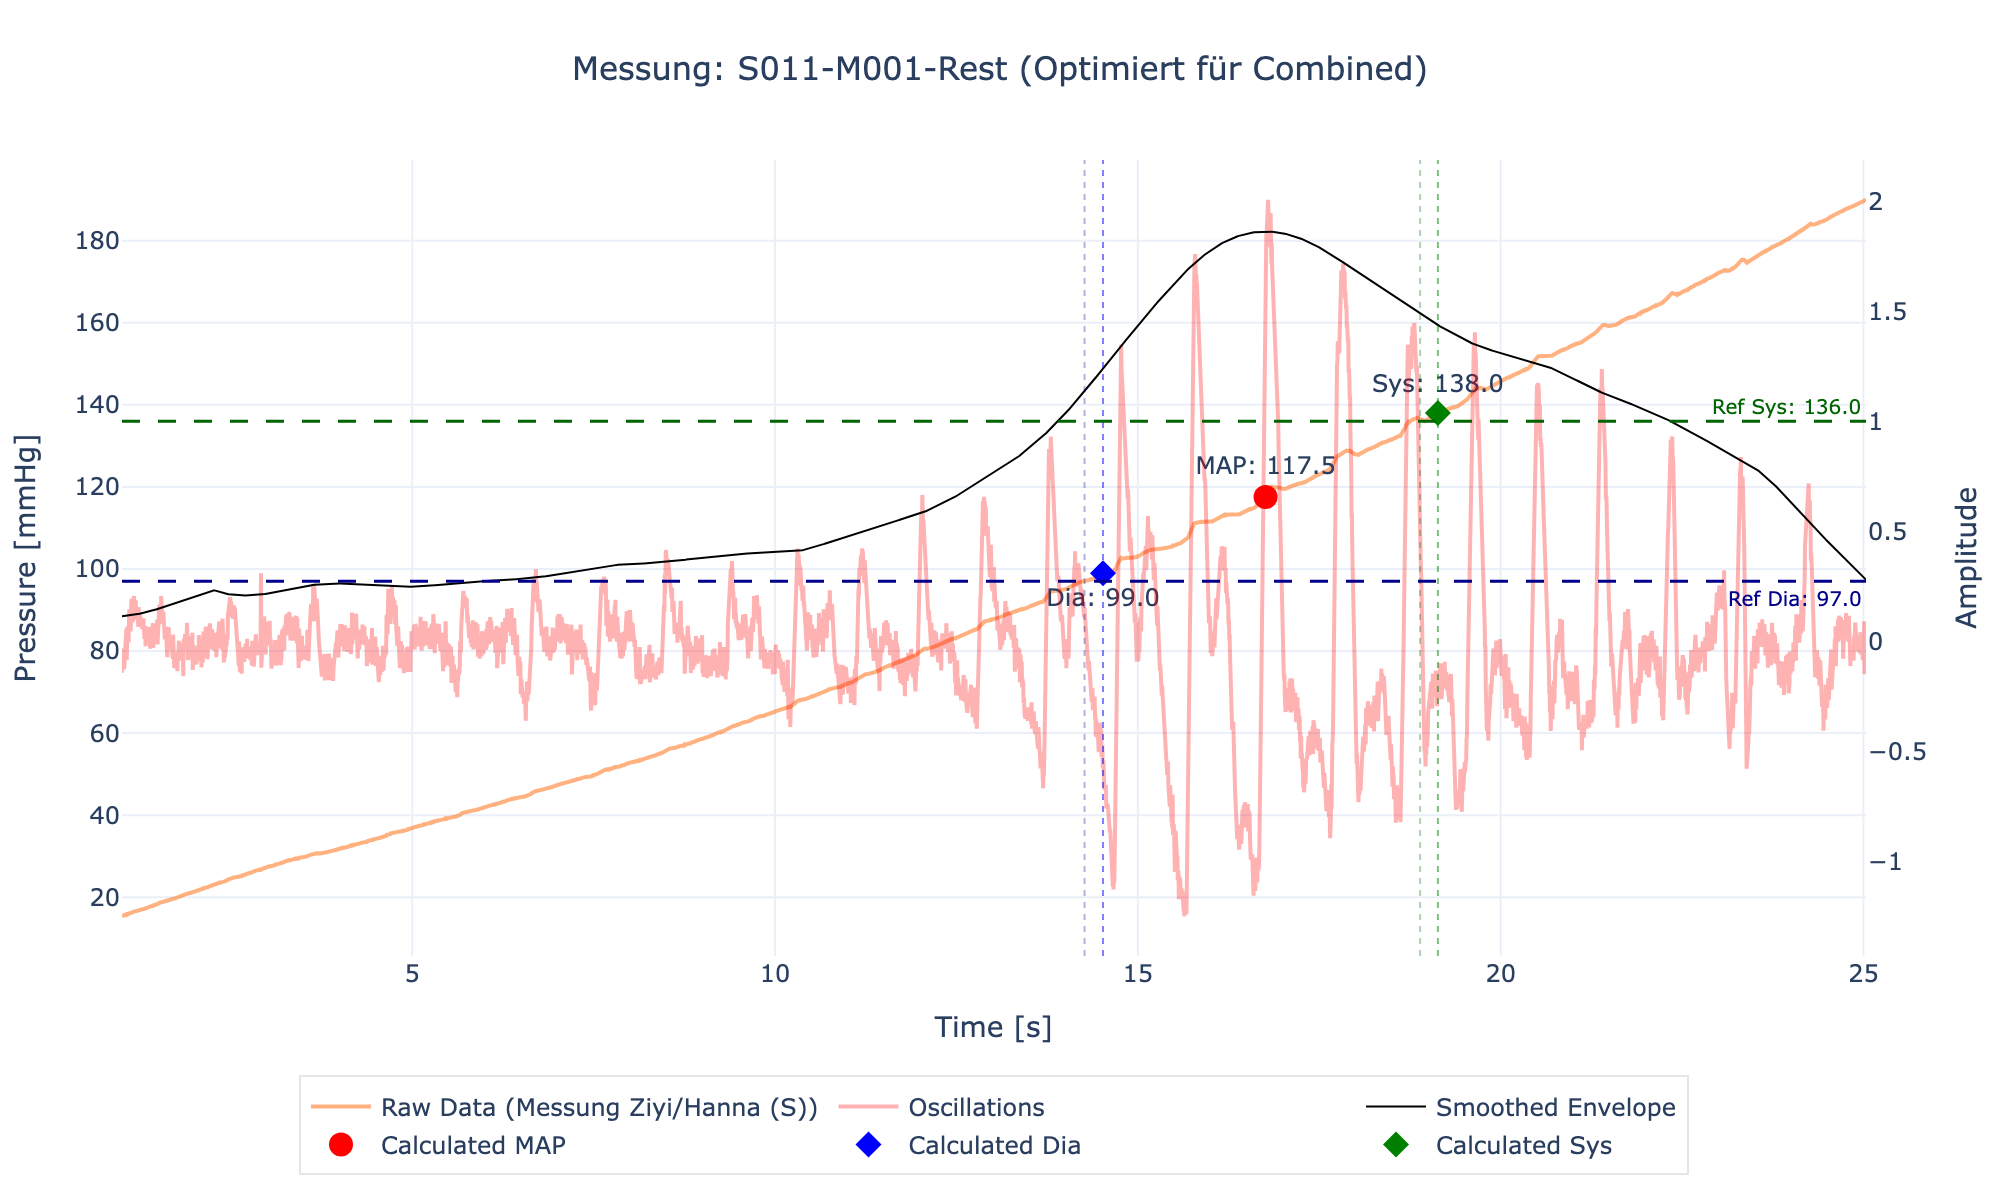
\includegraphics[width=\textwidth]{images/S011-M001-Rest_combined.png}
        \caption{Optimiert für Beurer und NAIS (Kombiniert)}
    \end{subfigure} \\
    \begin{subfigure}[b]{0.48\textwidth}
        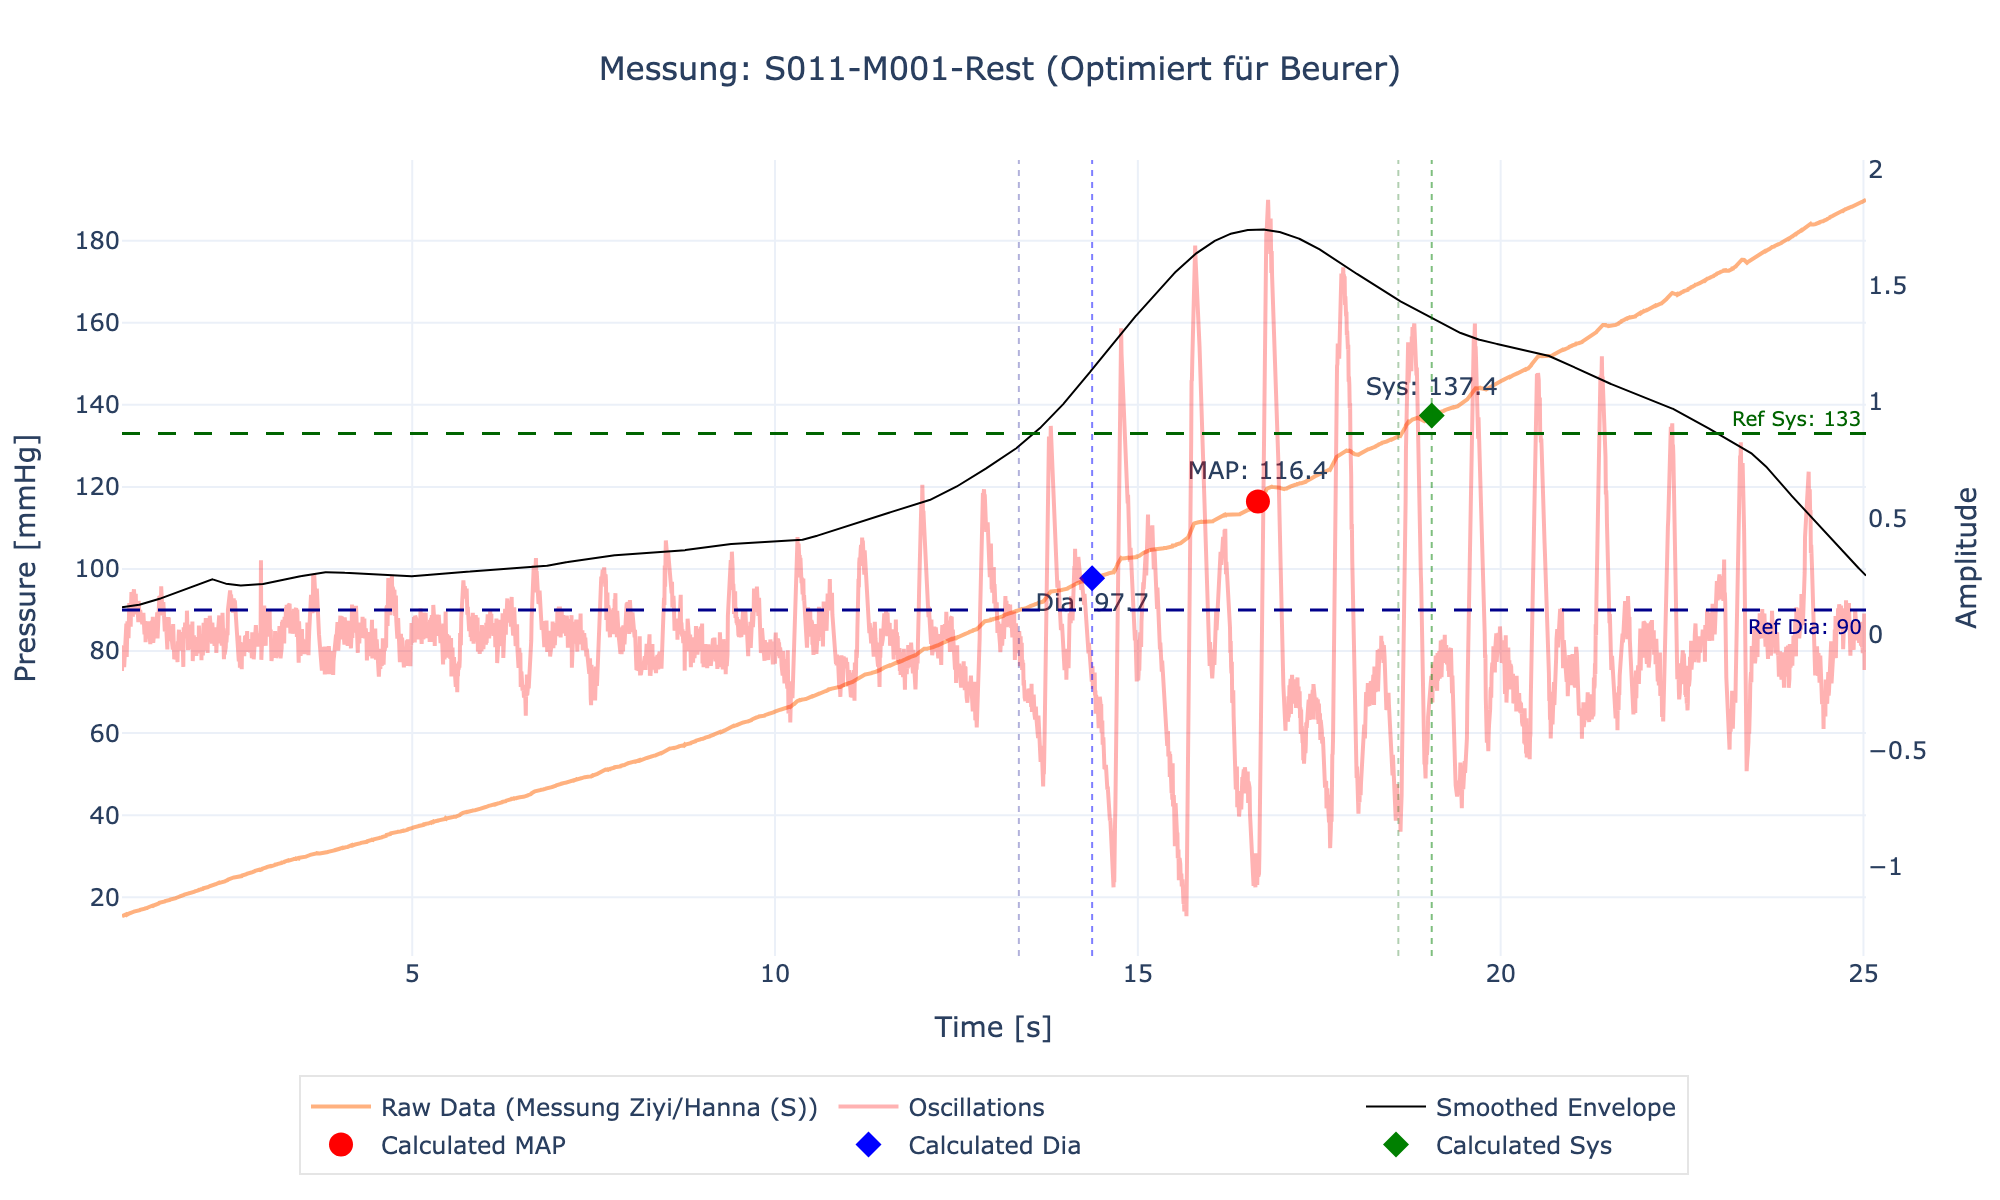
\includegraphics[width=\textwidth]{images/S011-M001-Rest_beurer.png}
        \caption{Optimiert für Beurer}
    \end{subfigure}
    \hfill
    \begin{subfigure}[b]{0.48\textwidth}
        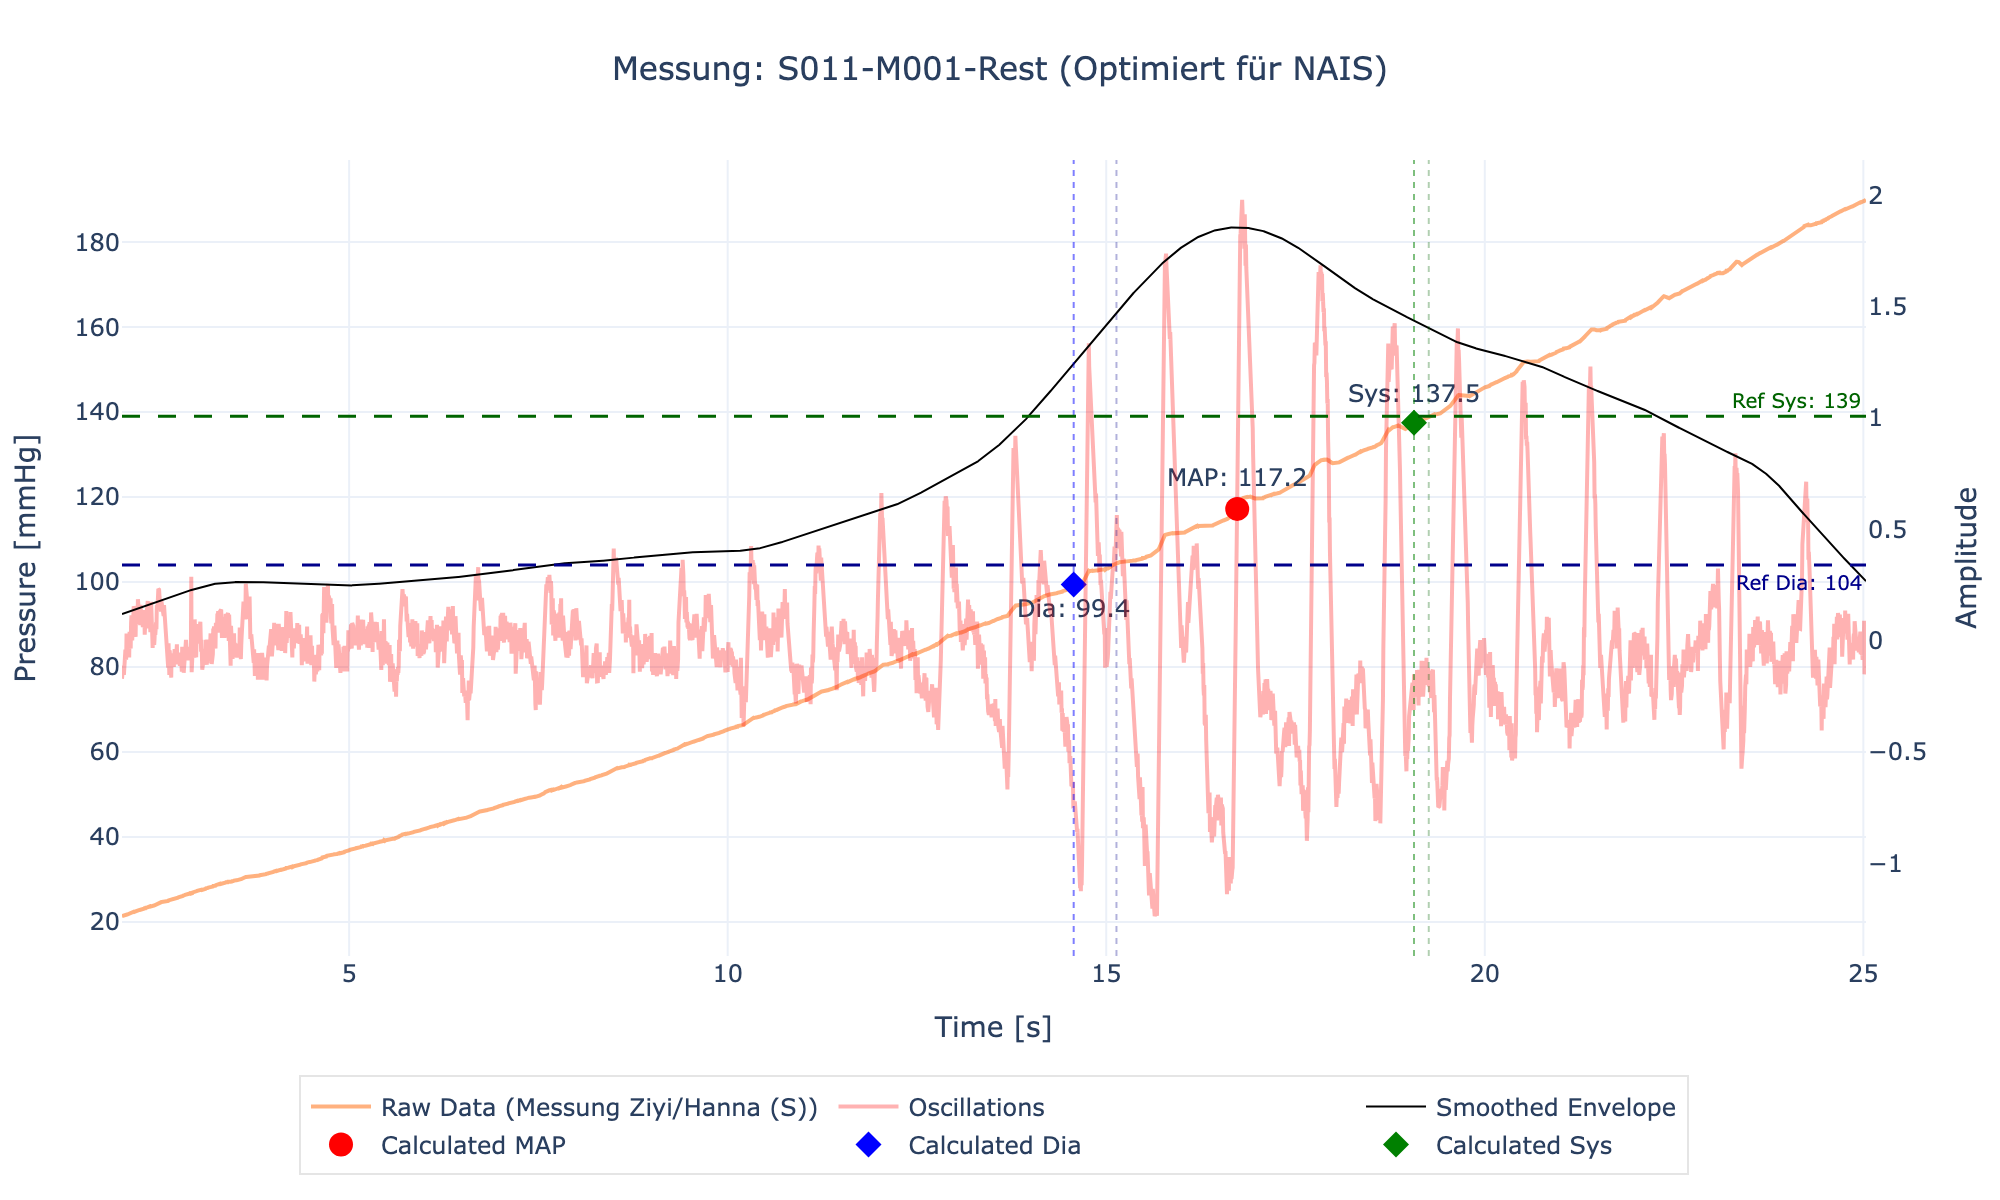
\includegraphics[width=\textwidth]{images/S011-M001-Rest_nais.png}
        \caption{Optimiert für NAIS}
    \end{subfigure}
    \caption{Einzelauswertung der Messung S011-M001-Rest mit verschiedenen Parametersätzen.}
\end{figure}
\newpage

\subsection*{Messung: S011-M002-Active}
\begin{figure}[H]
    \centering
    \begin{subfigure}[b]{0.8\textwidth}
        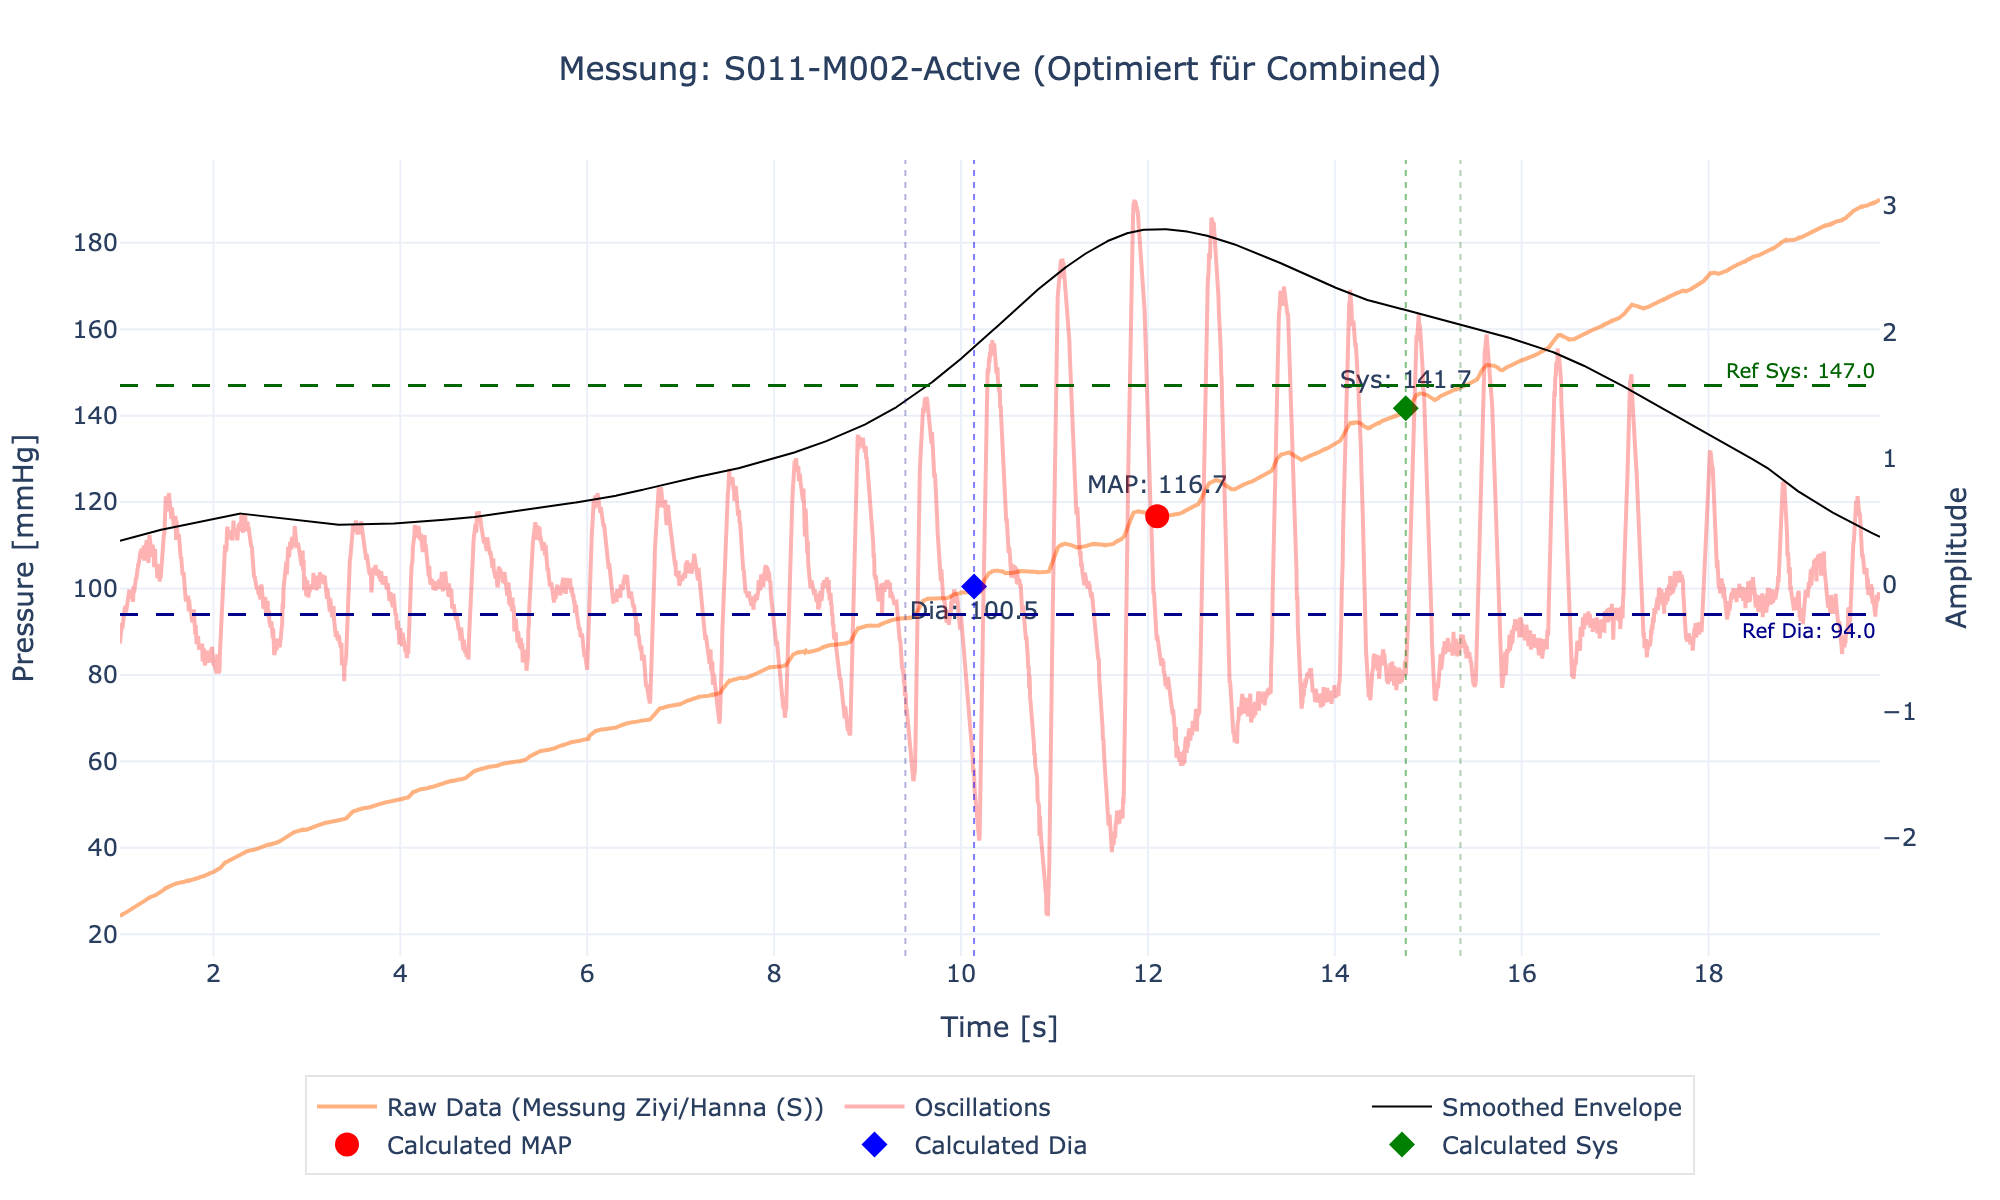
\includegraphics[width=\textwidth]{images/S011-M002-Active_combined.png}
        \caption{Optimiert für Beurer und NAIS (Kombiniert)}
    \end{subfigure} \\
    \begin{subfigure}[b]{0.48\textwidth}
        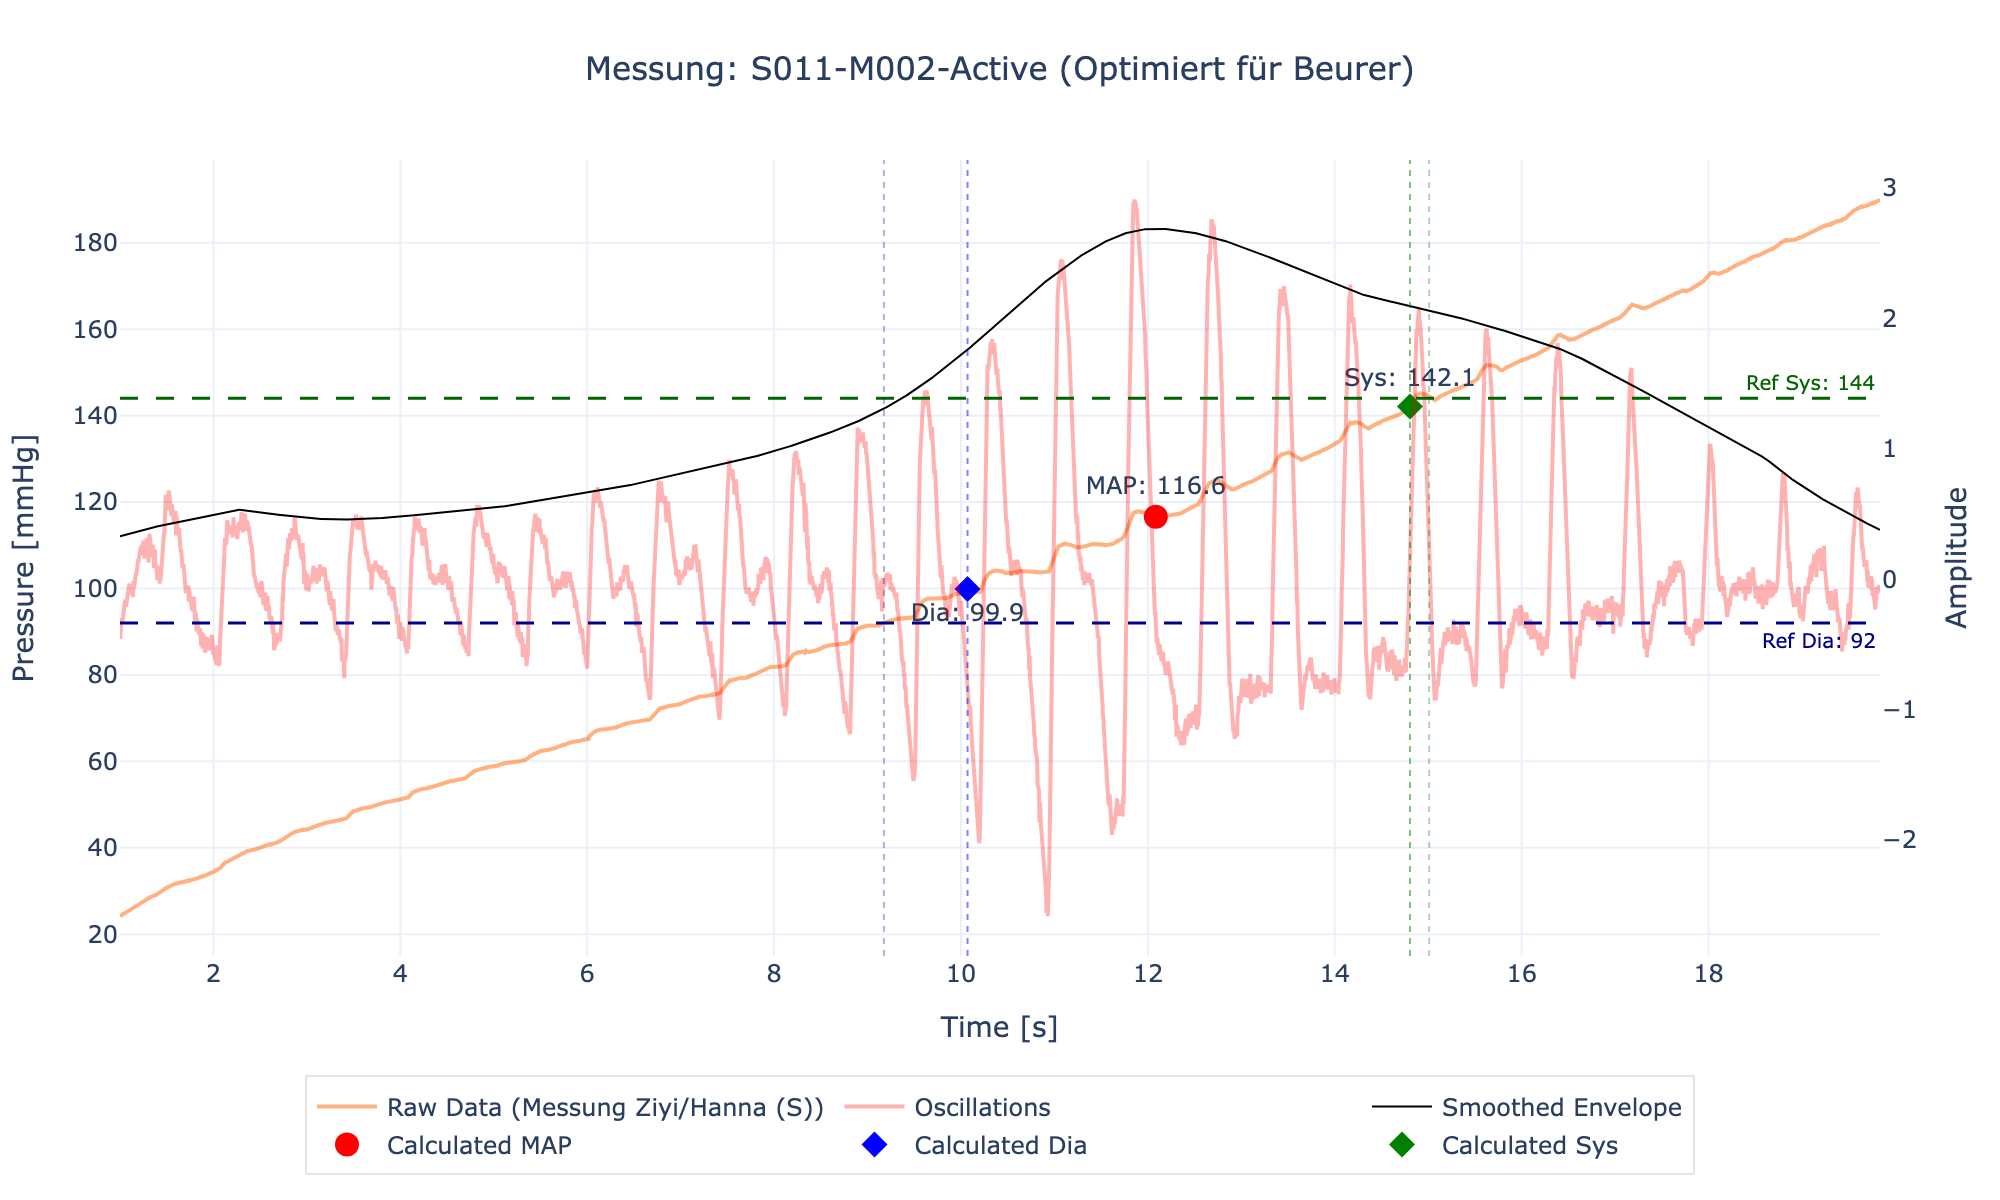
\includegraphics[width=\textwidth]{images/S011-M002-Active_beurer.png}
        \caption{Optimiert für Beurer}
    \end{subfigure}
    \hfill
    \begin{subfigure}[b]{0.48\textwidth}
        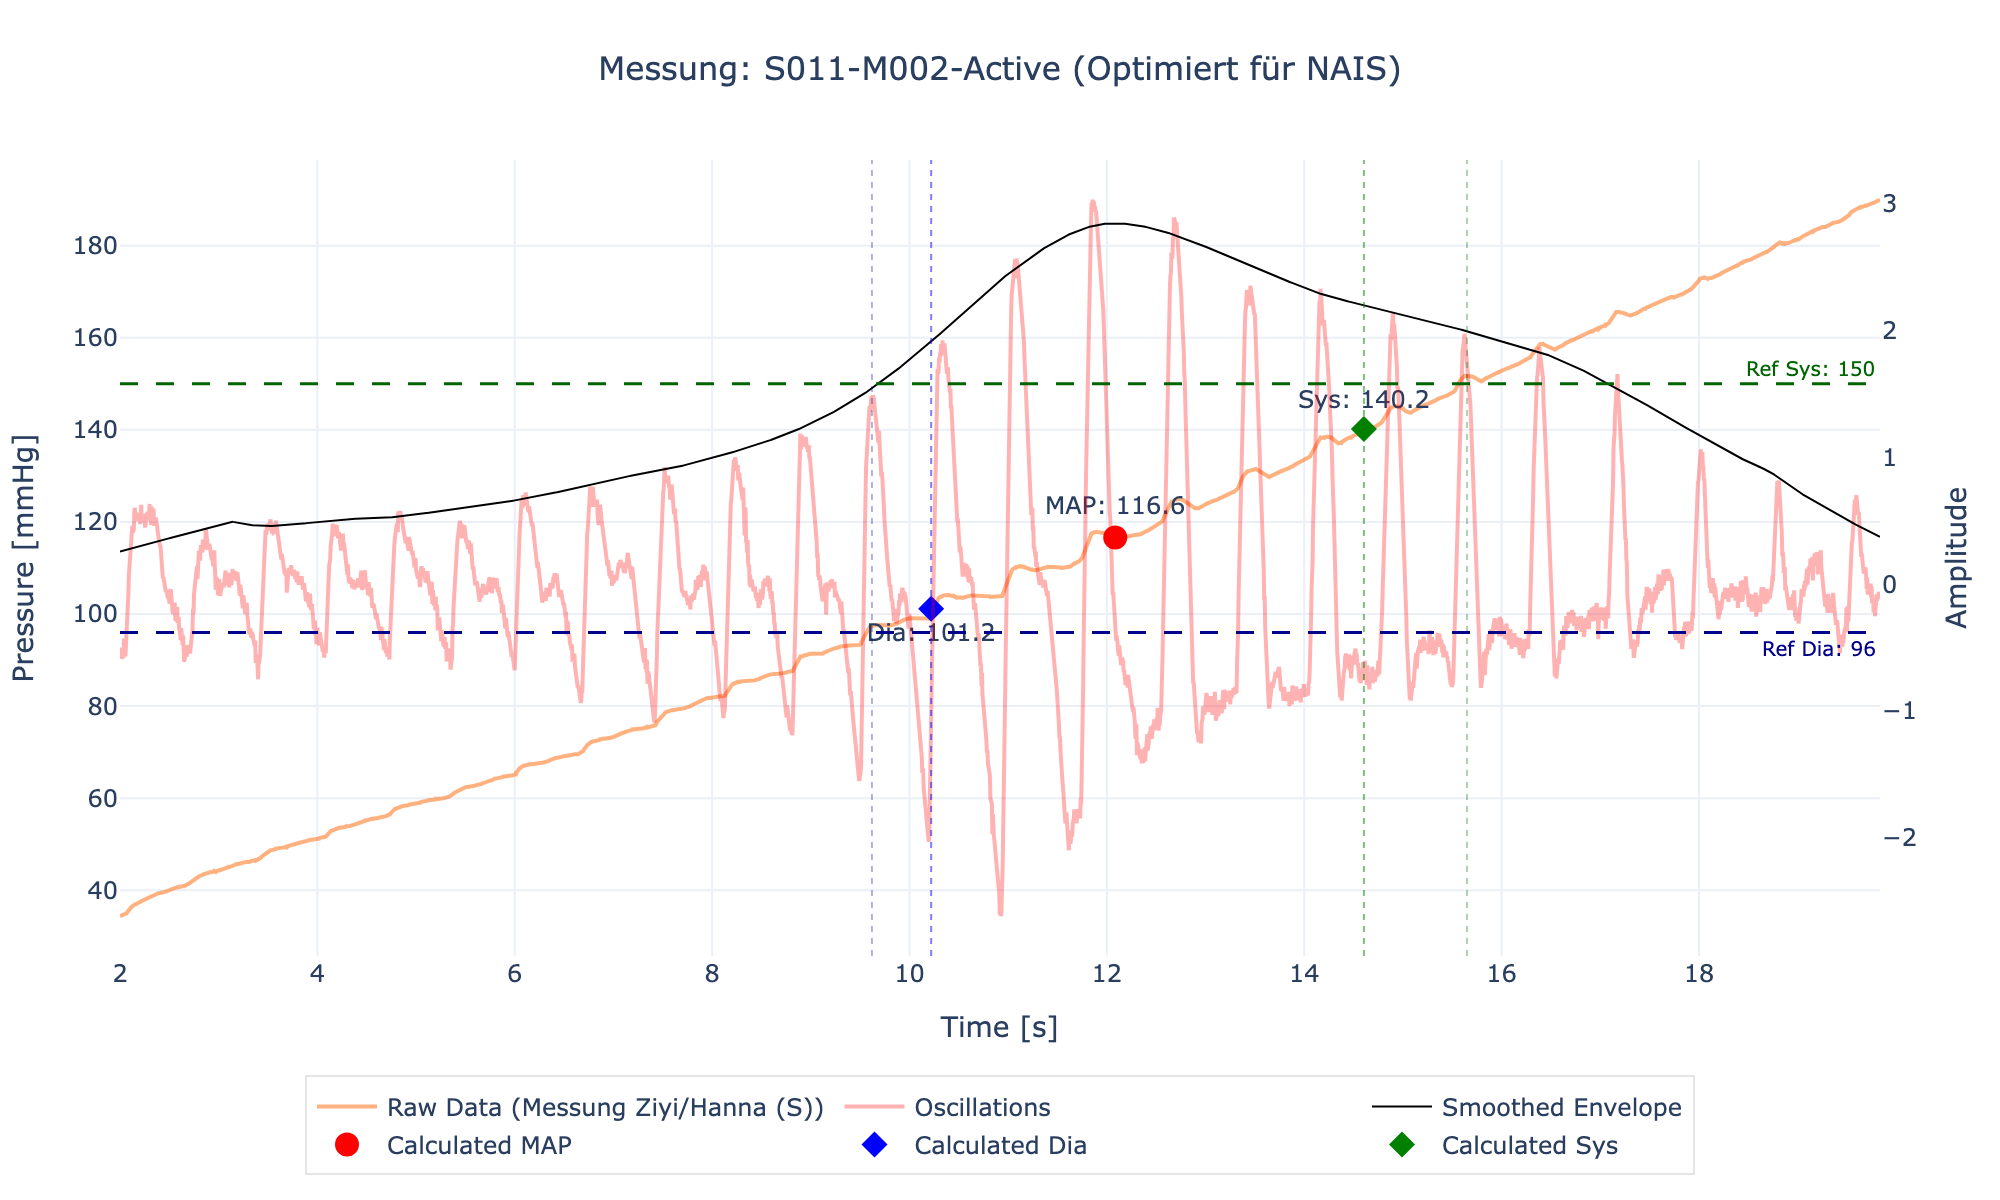
\includegraphics[width=\textwidth]{images/S011-M002-Active_nais.png}
        \caption{Optimiert für NAIS}
    \end{subfigure}
    \caption{Einzelauswertung der Messung S011-M002-Active mit verschiedenen Parametersätzen.}
\end{figure}
\newpage

\subsection*{Messung: S012-M001-Rest}
\begin{figure}[H]
    \centering
    \begin{subfigure}[b]{0.8\textwidth}
        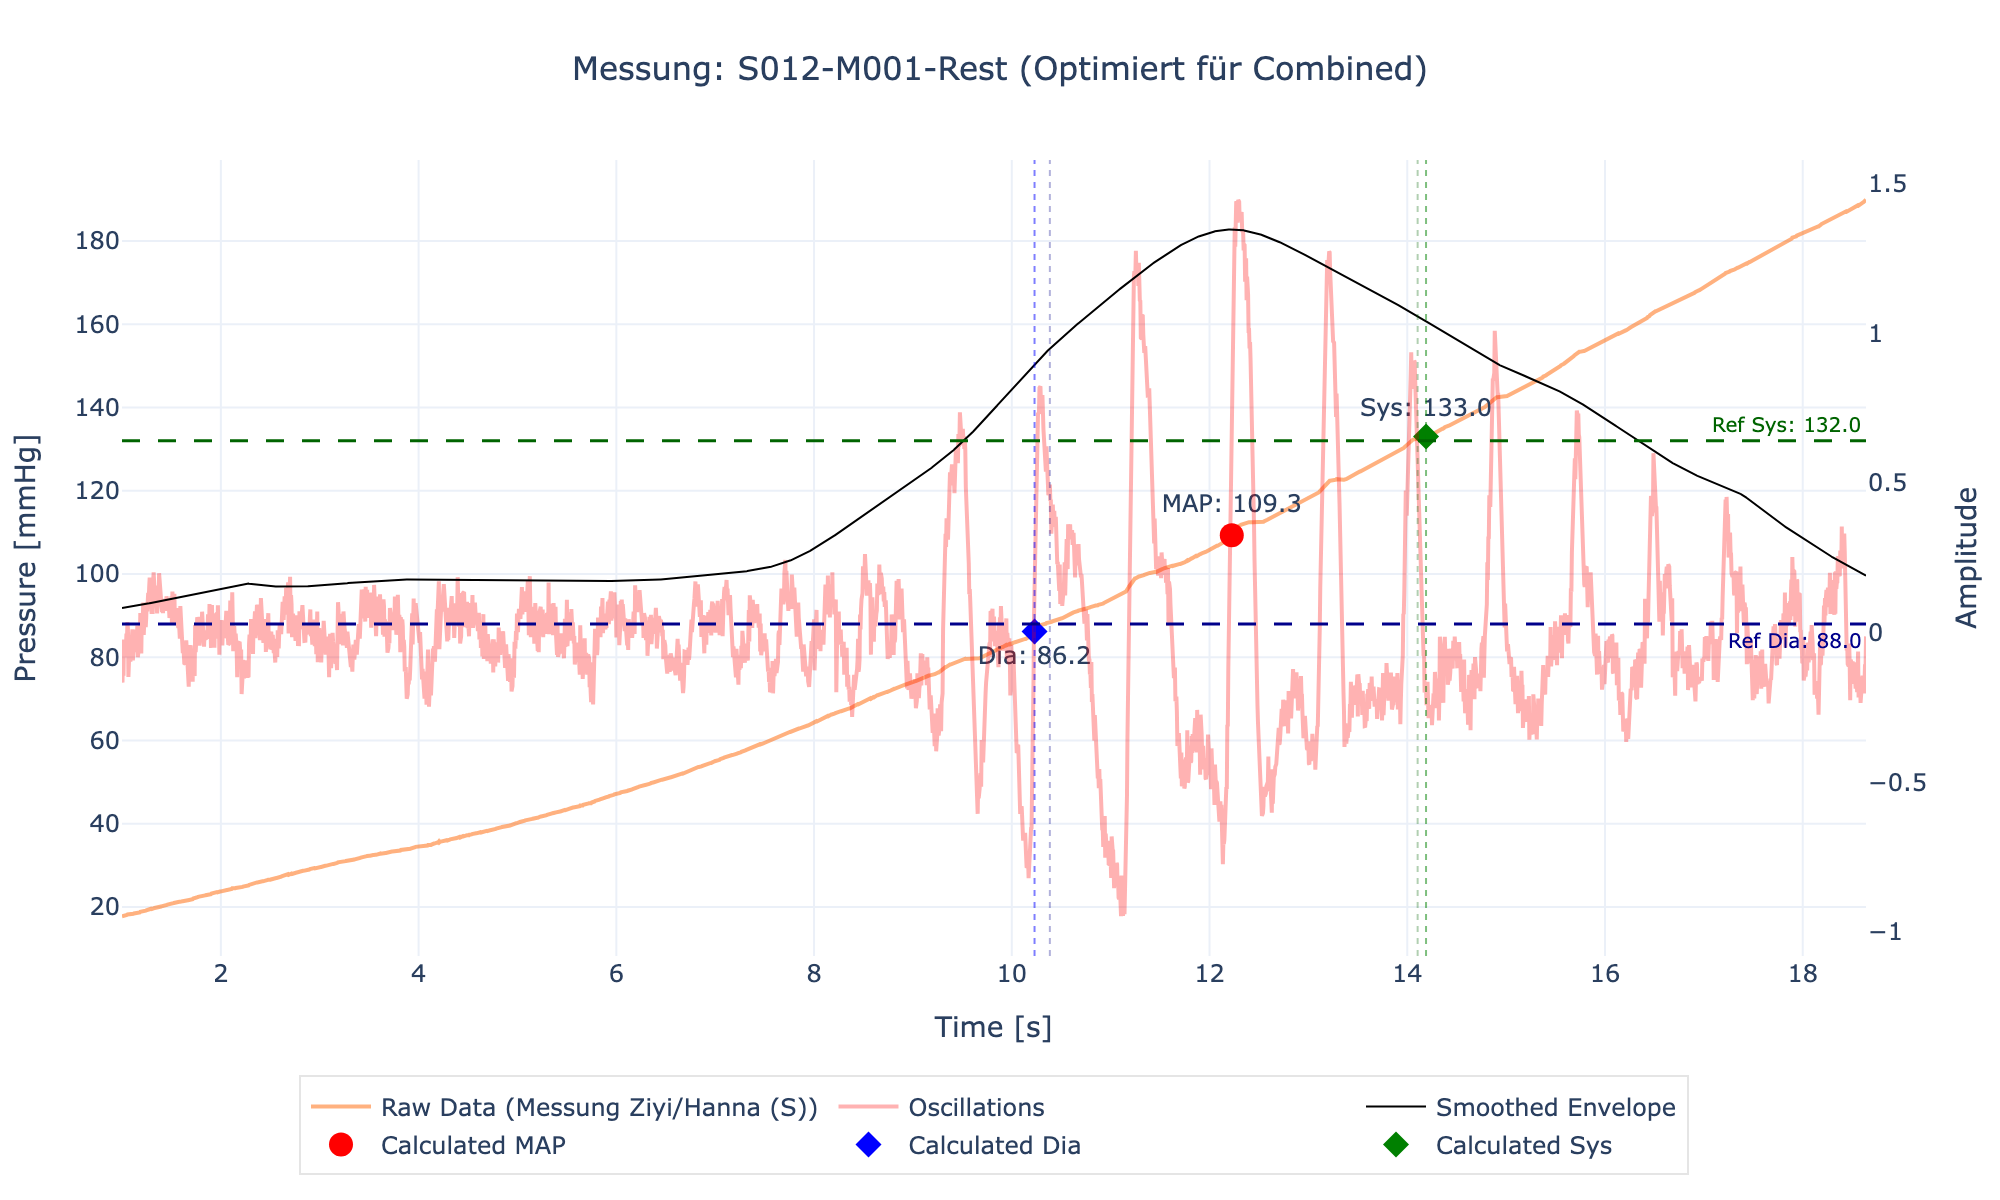
\includegraphics[width=\textwidth]{images/S012-M001-Rest_combined.png}
        \caption{Optimiert für Beurer und NAIS (Kombiniert)}
    \end{subfigure} \\
    \begin{subfigure}[b]{0.48\textwidth}
        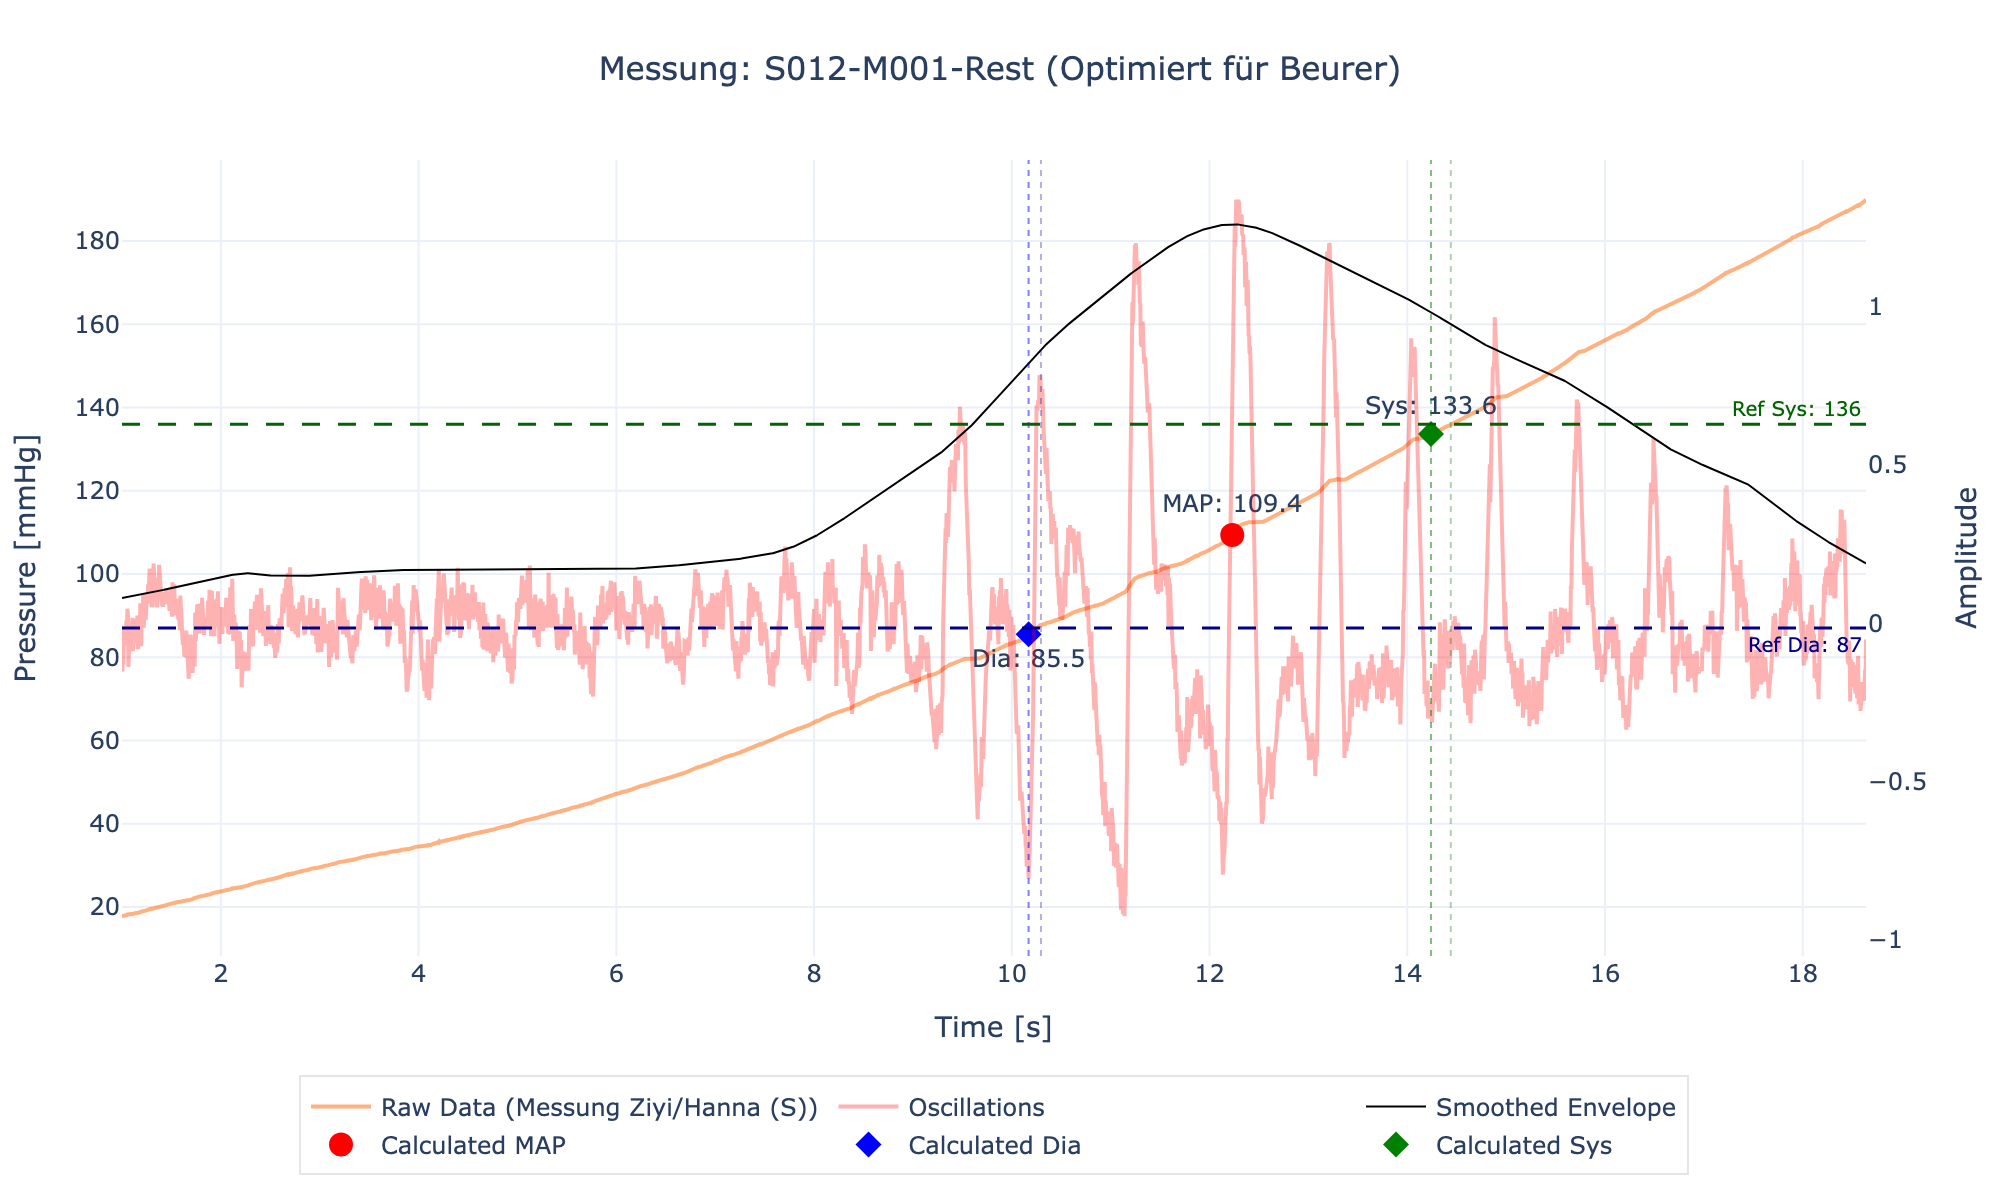
\includegraphics[width=\textwidth]{images/S012-M001-Rest_beurer.png}
        \caption{Optimiert für Beurer}
    \end{subfigure}
    \hfill
    \begin{subfigure}[b]{0.48\textwidth}
        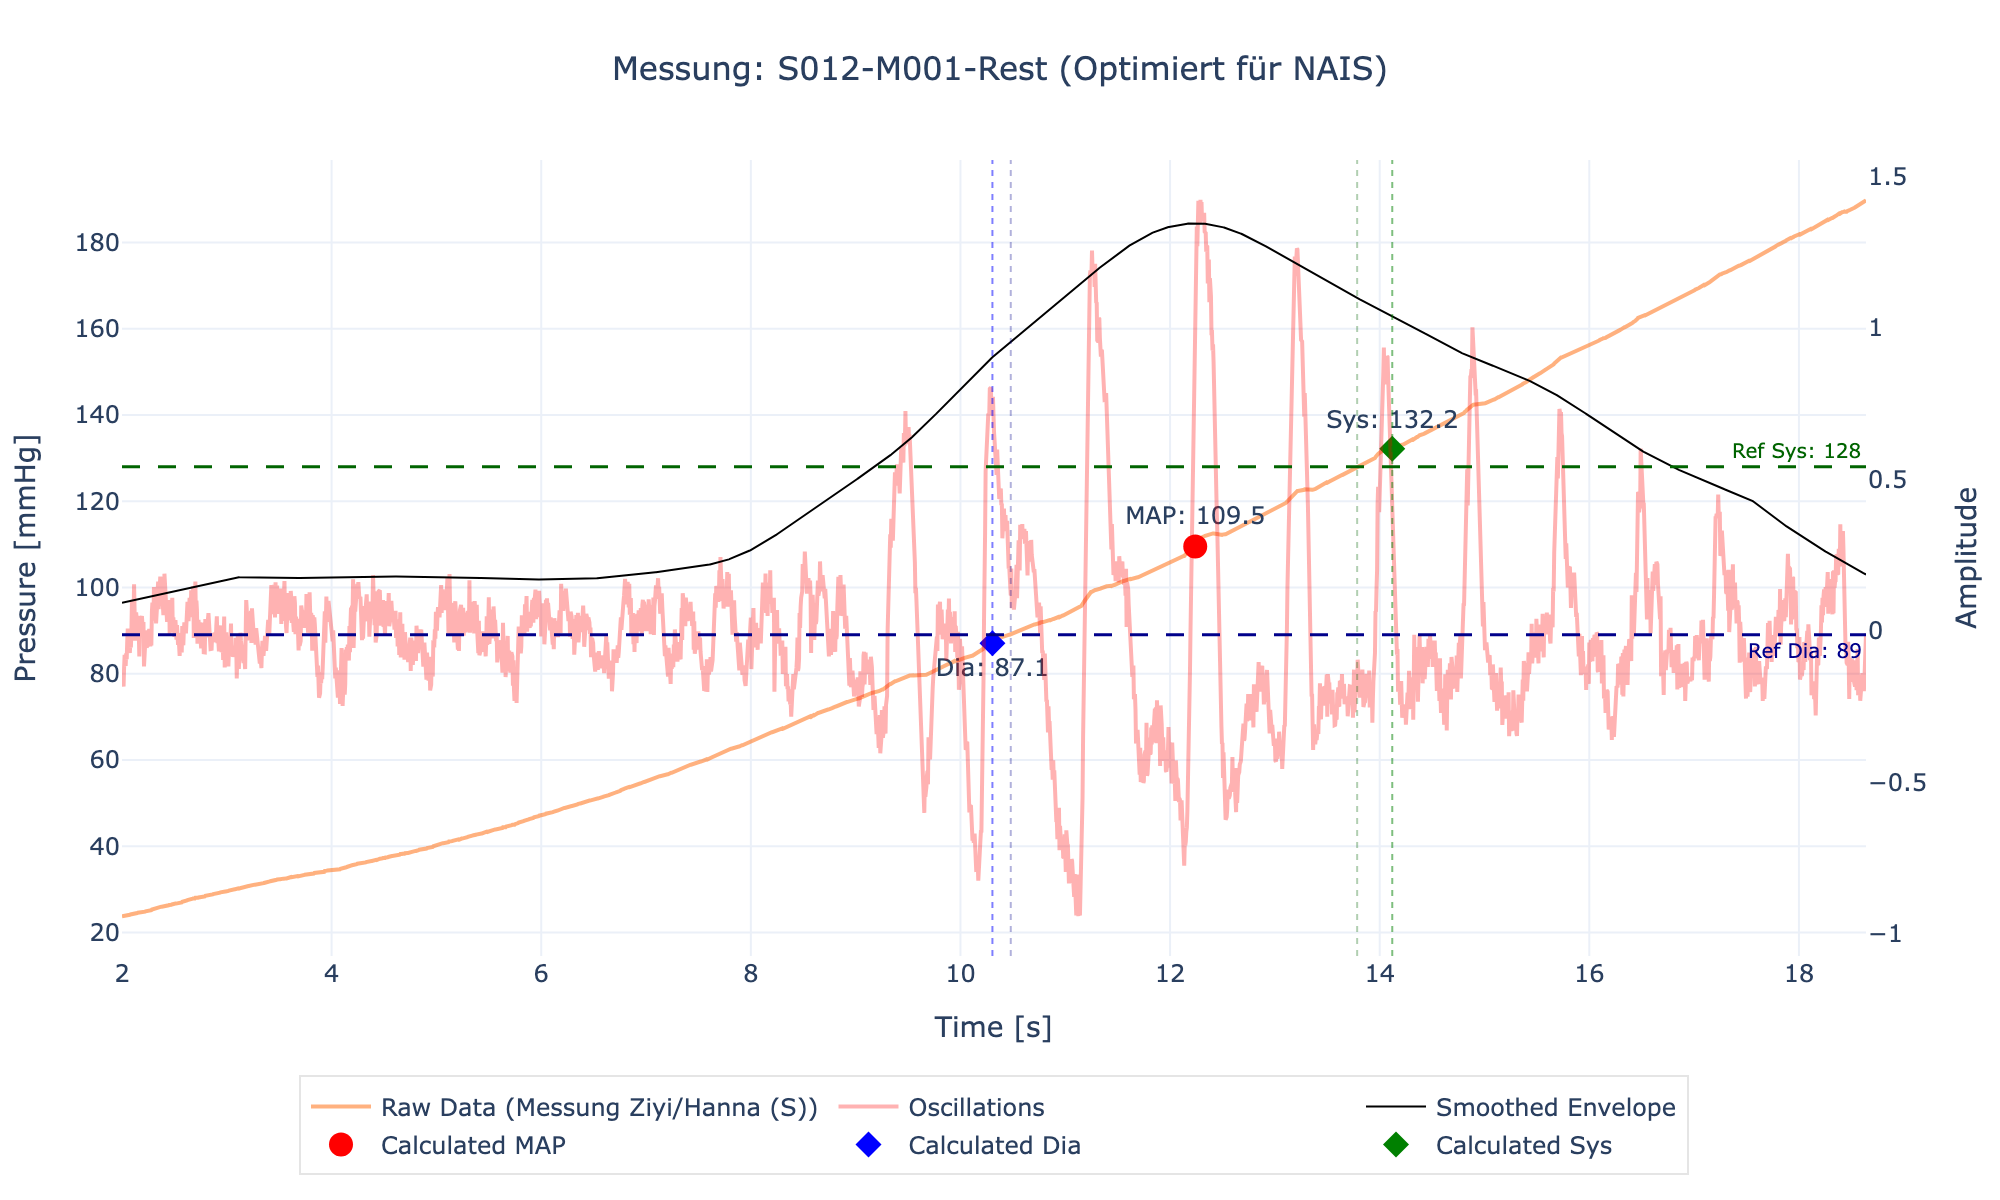
\includegraphics[width=\textwidth]{images/S012-M001-Rest_nais.png}
        \caption{Optimiert für NAIS}
    \end{subfigure}
    \caption{Einzelauswertung der Messung S012-M001-Rest mit verschiedenen Parametersätzen.}
\end{figure}
\newpage

\subsection*{Messung: S012-M002-Active}
\begin{figure}[H]
    \centering
    \begin{subfigure}[b]{0.8\textwidth}
        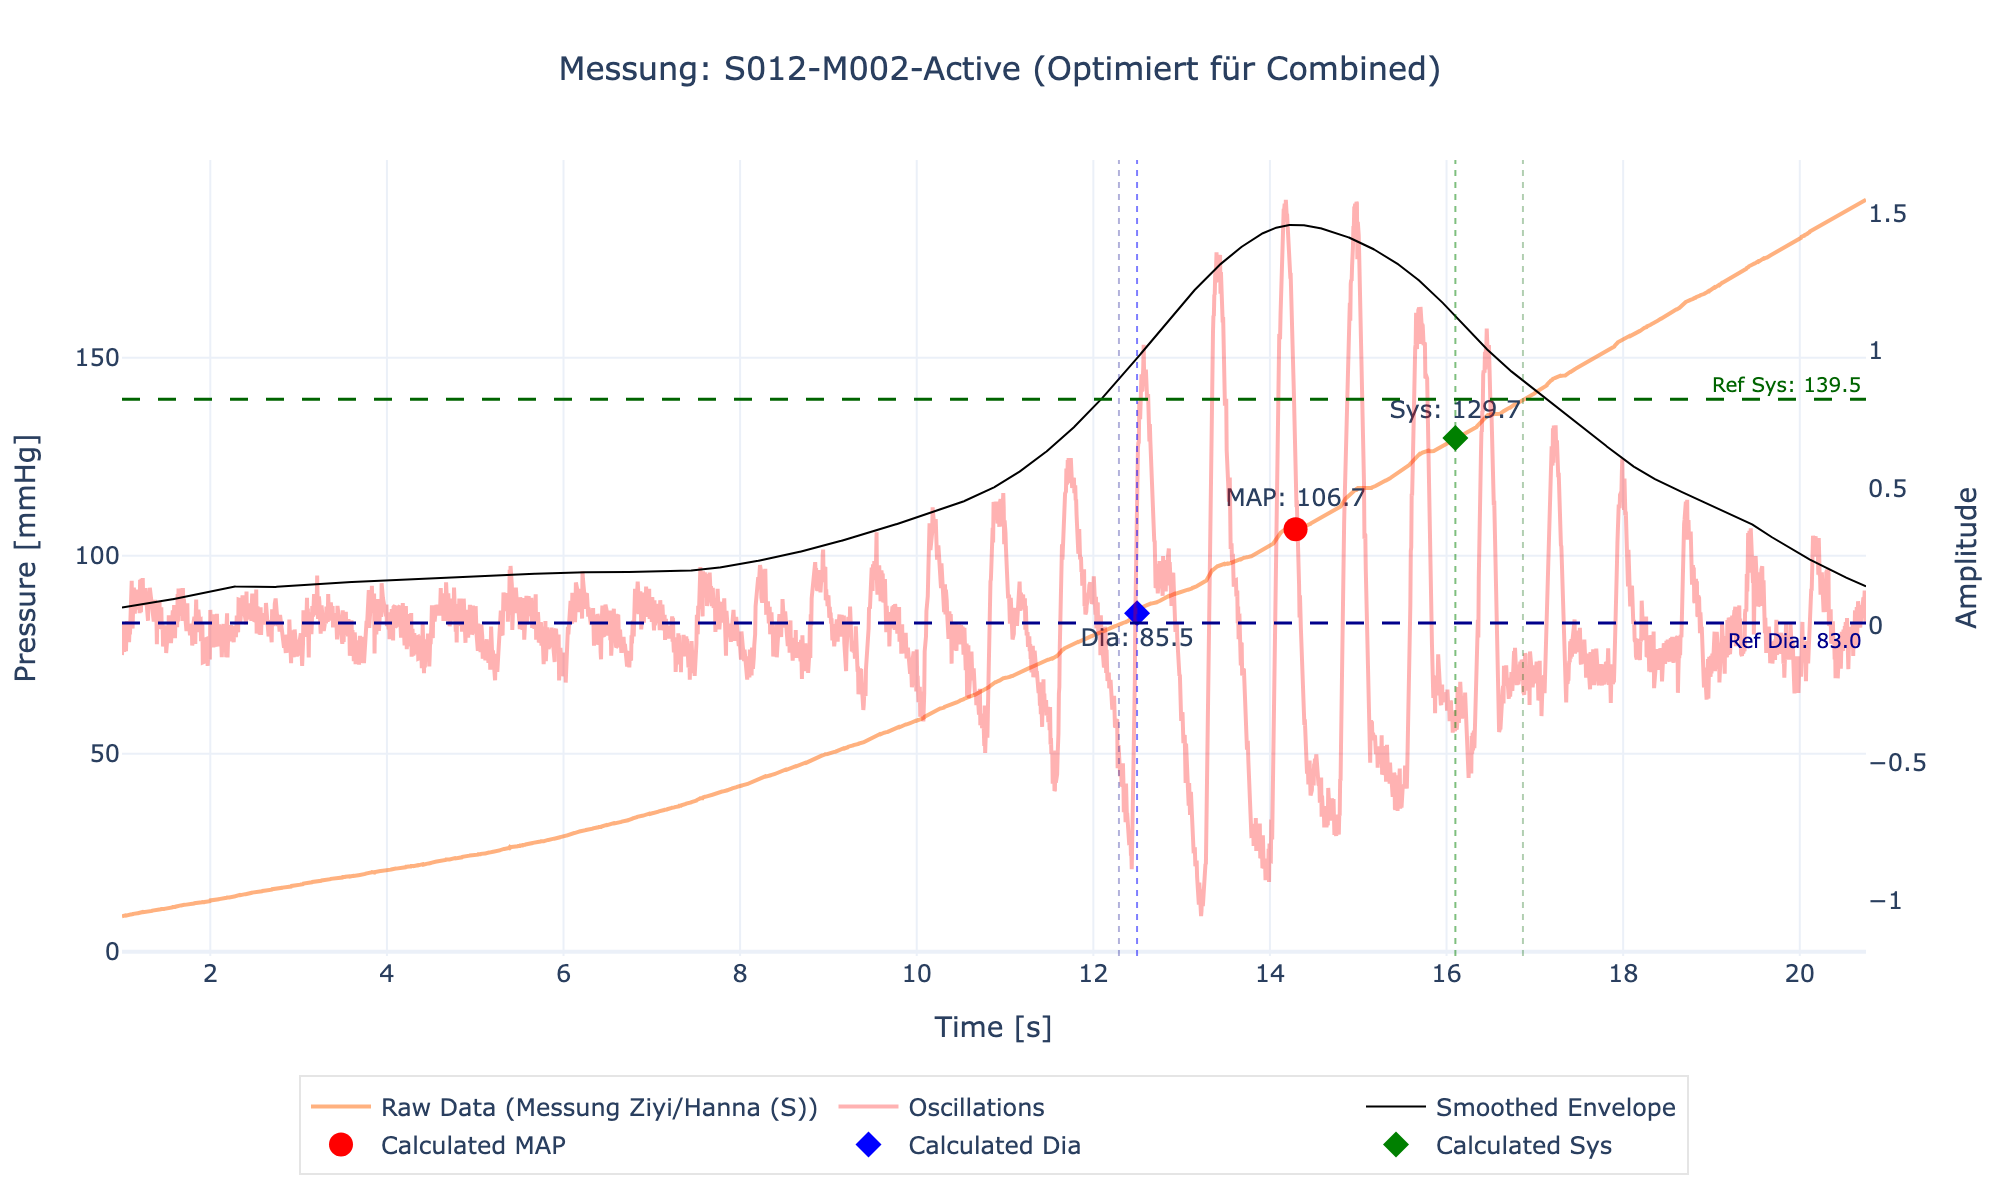
\includegraphics[width=\textwidth]{images/S012-M002-Active_combined.png}
        \caption{Optimiert für Beurer und NAIS (Kombiniert)}
    \end{subfigure} \\
    \begin{subfigure}[b]{0.48\textwidth}
        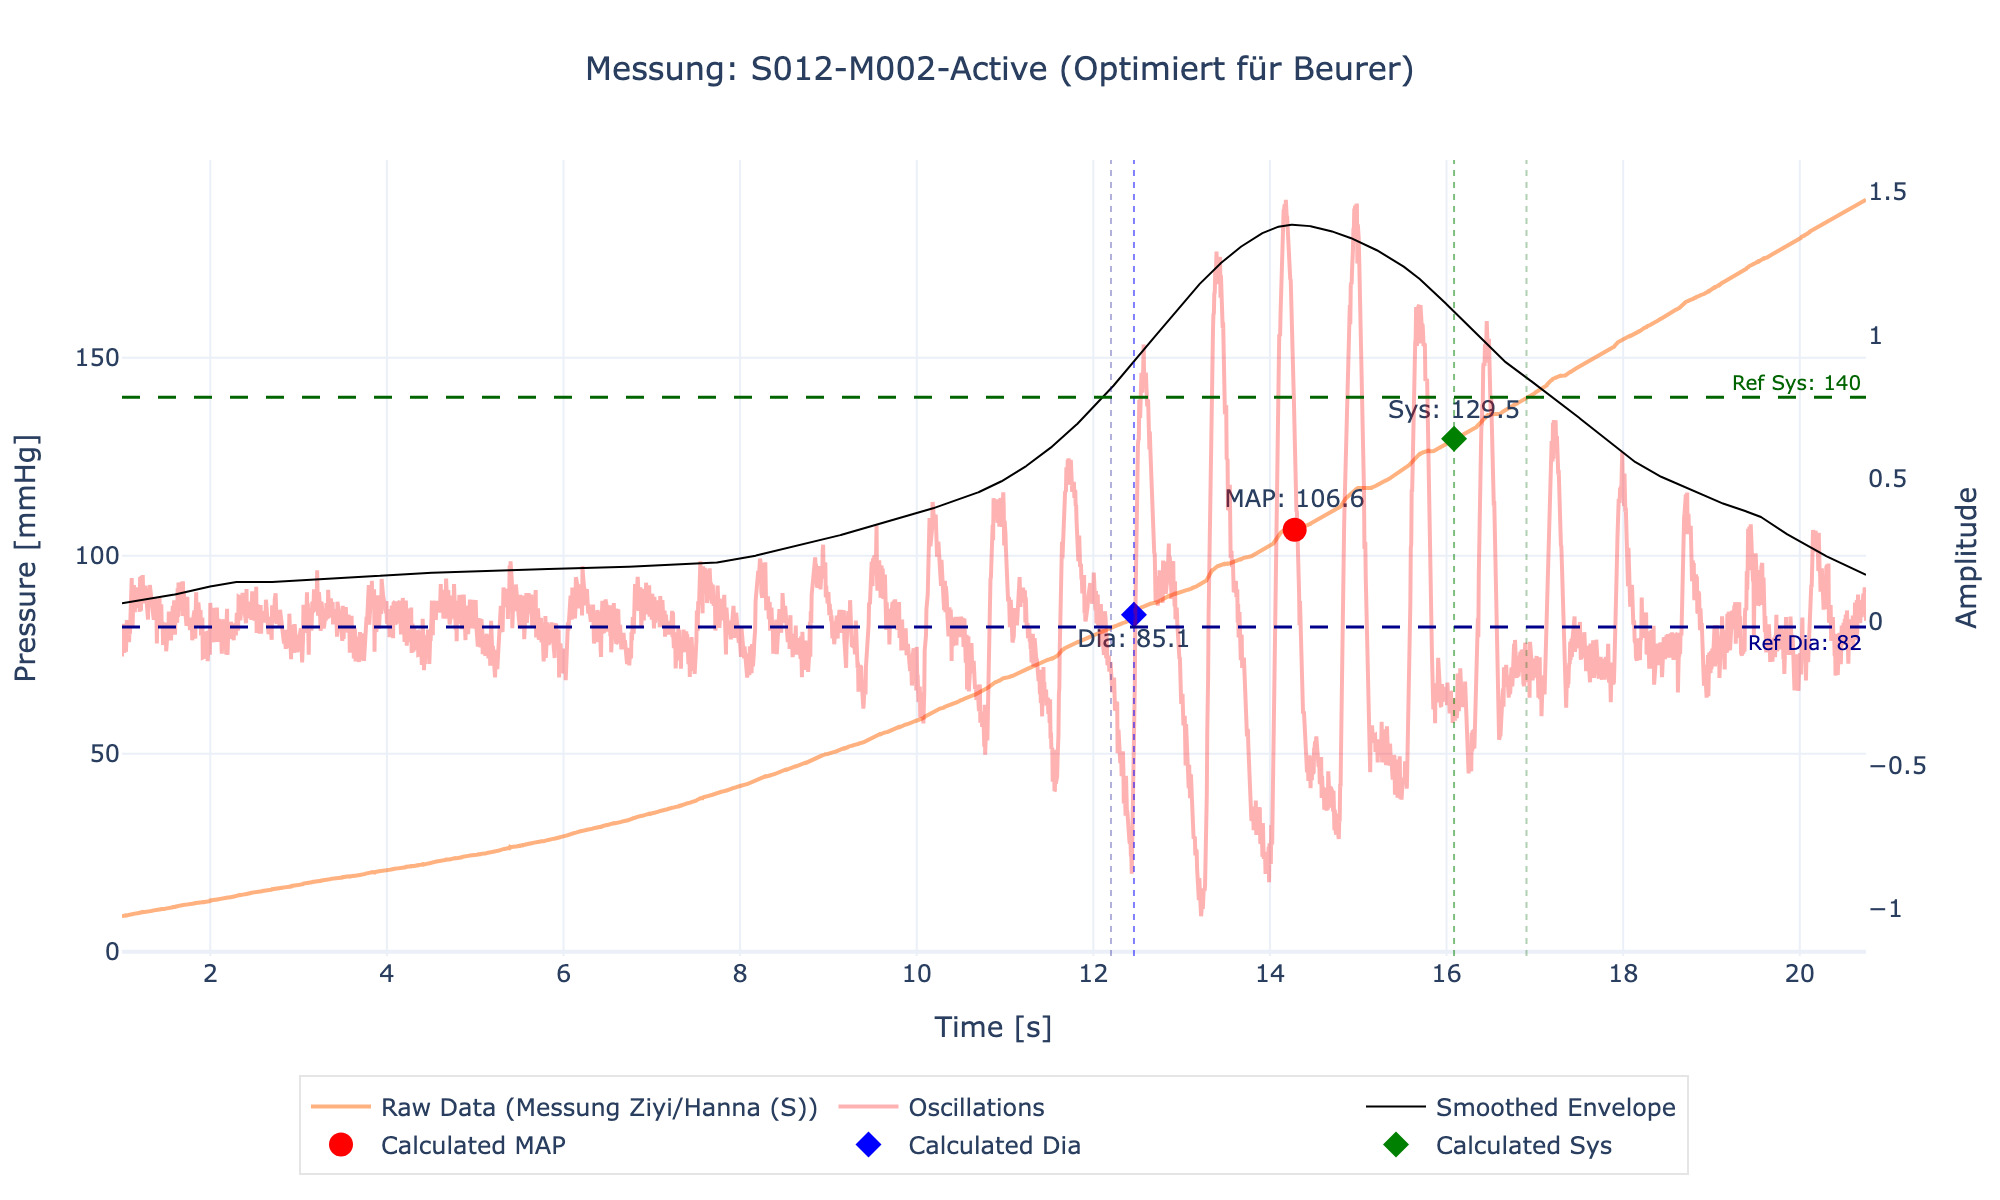
\includegraphics[width=\textwidth]{images/S012-M002-Active_beurer.png}
        \caption{Optimiert für Beurer}
    \end{subfigure}
    \hfill
    \begin{subfigure}[b]{0.48\textwidth}
        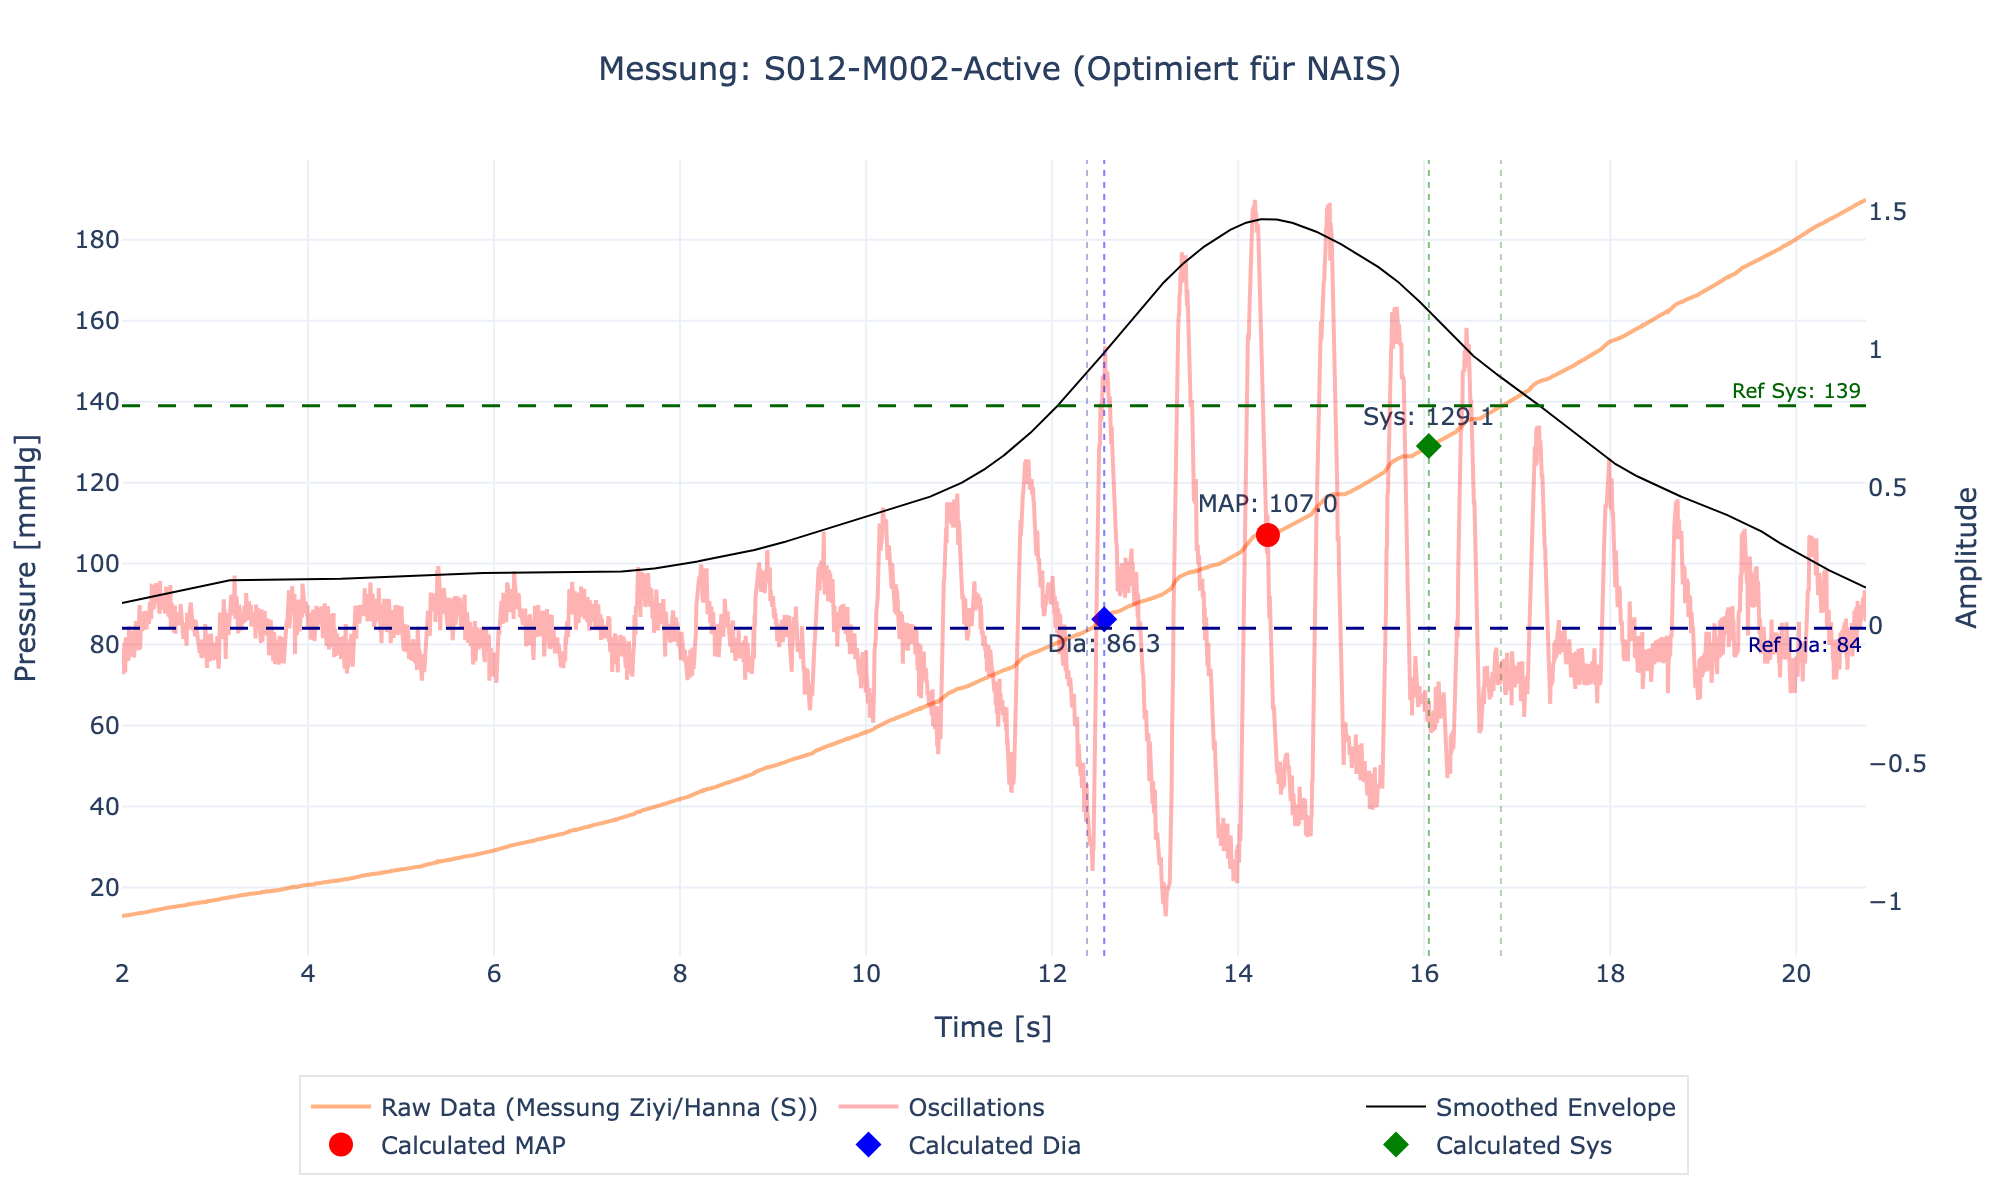
\includegraphics[width=\textwidth]{images/S012-M002-Active_nais.png}
        \caption{Optimiert für NAIS}
    \end{subfigure}
    \caption{Einzelauswertung der Messung S012-M002-Active mit verschiedenen Parametersätzen.}
\end{figure}
\newpage

\subsection*{Messung: S013-M001-Rest}
\begin{figure}[H]
    \centering
    \begin{subfigure}[b]{0.8\textwidth}
        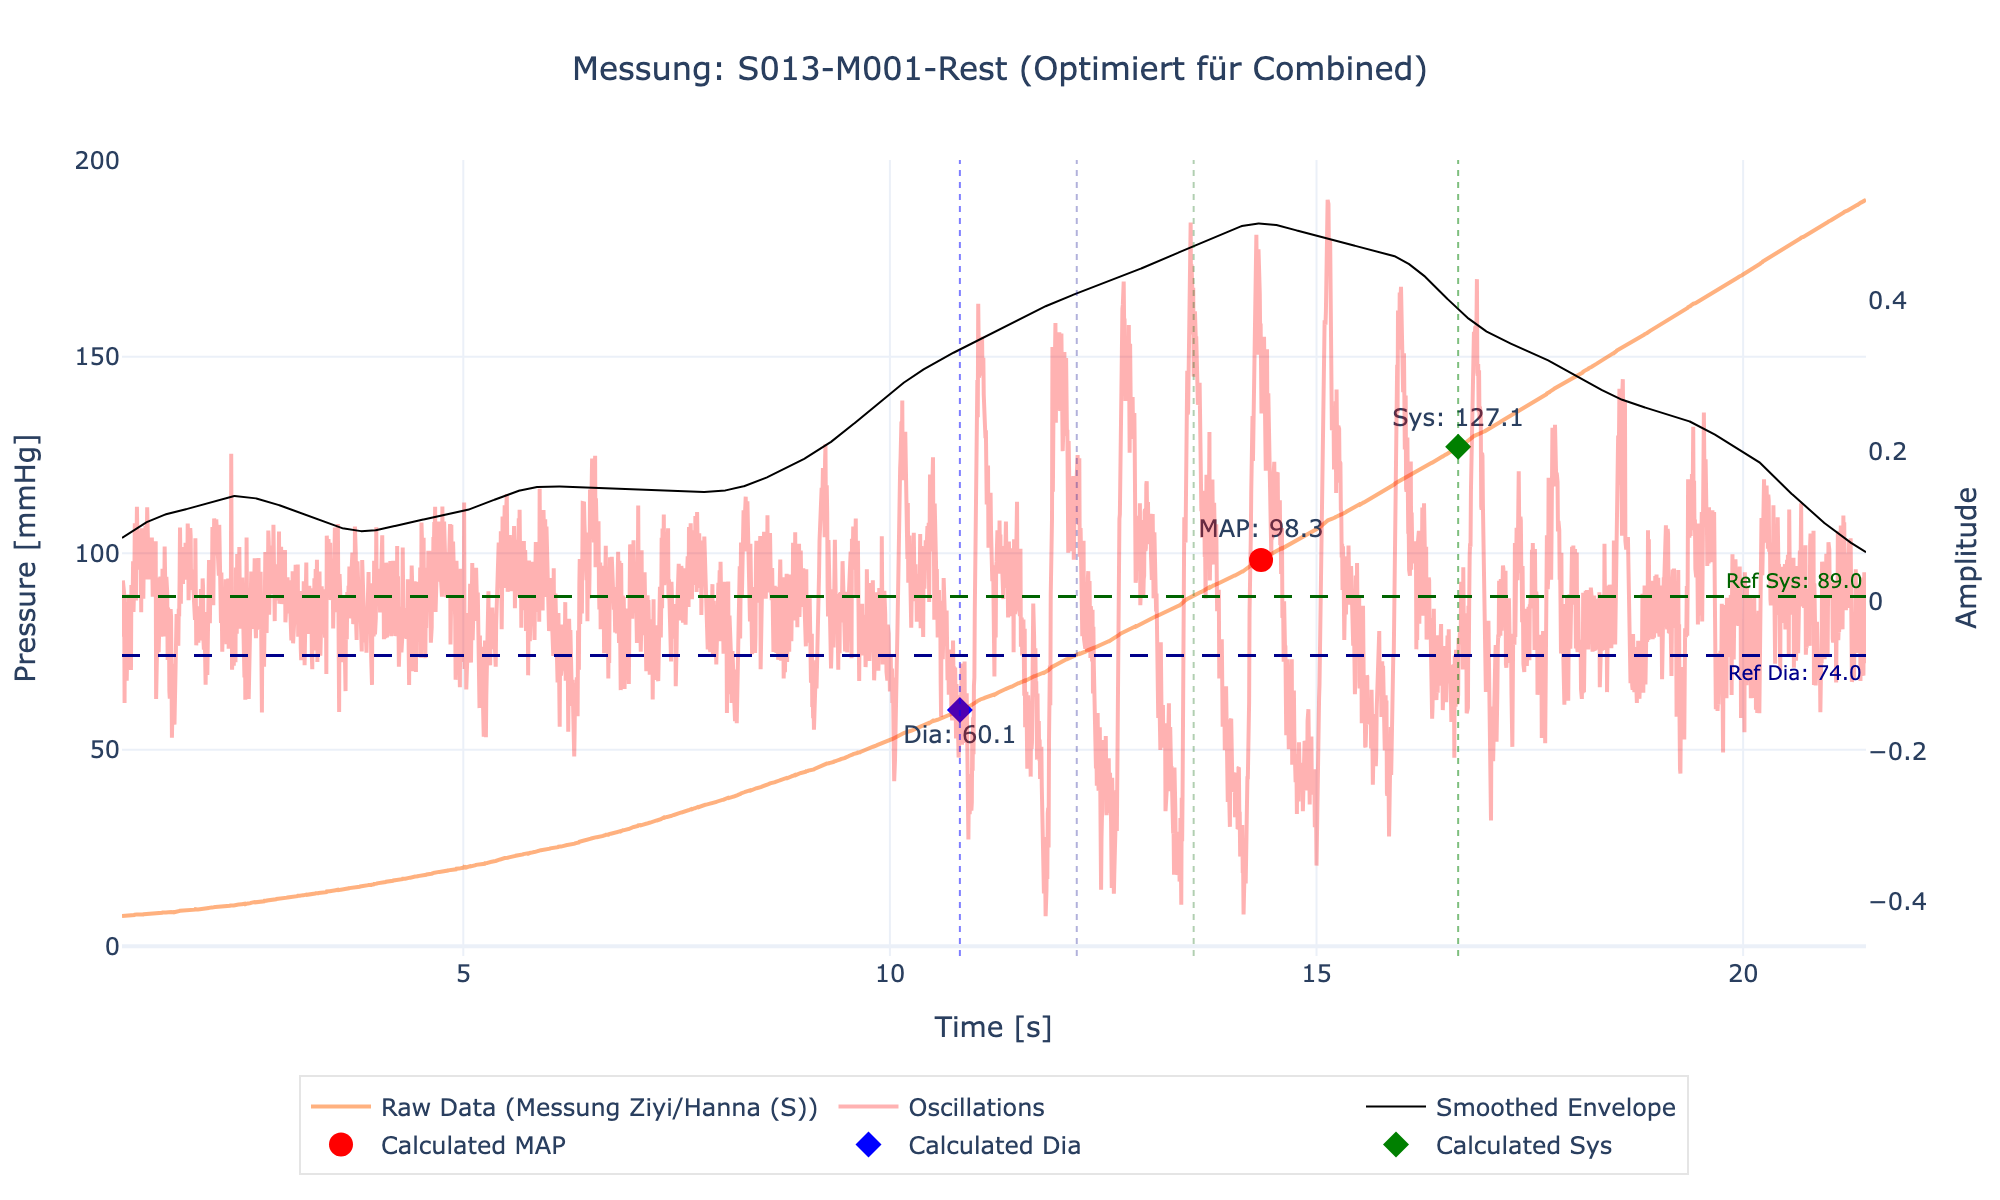
\includegraphics[width=\textwidth]{images/S013-M001-Rest_combined.png}
        \caption{Optimiert für Beurer und NAIS (Kombiniert)}
    \end{subfigure} \\
    \begin{subfigure}[b]{0.48\textwidth}
        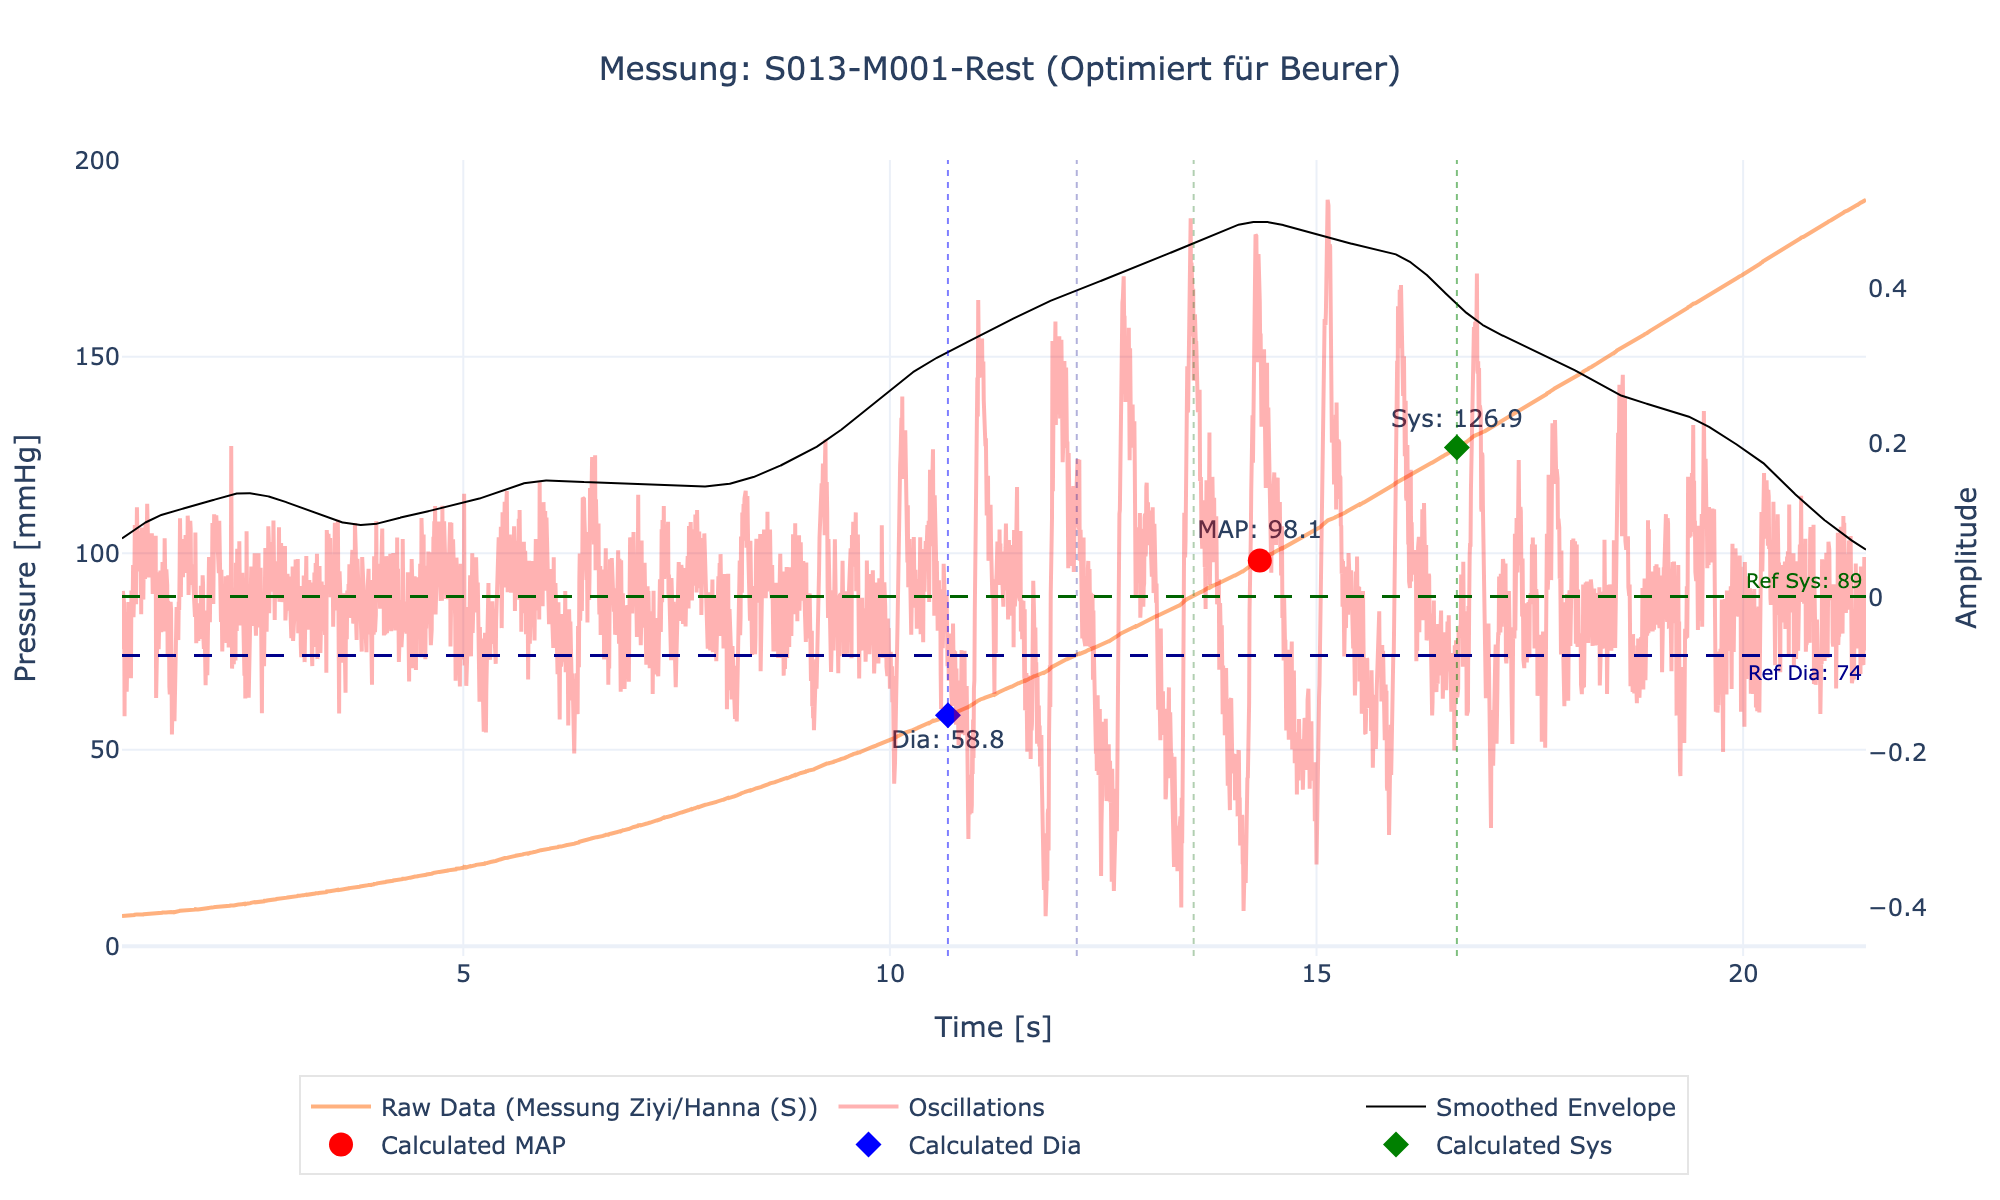
\includegraphics[width=\textwidth]{images/S013-M001-Rest_beurer.png}
        \caption{Optimiert für Beurer}
    \end{subfigure}
    \hfill
    \begin{subfigure}[b]{0.48\textwidth}
        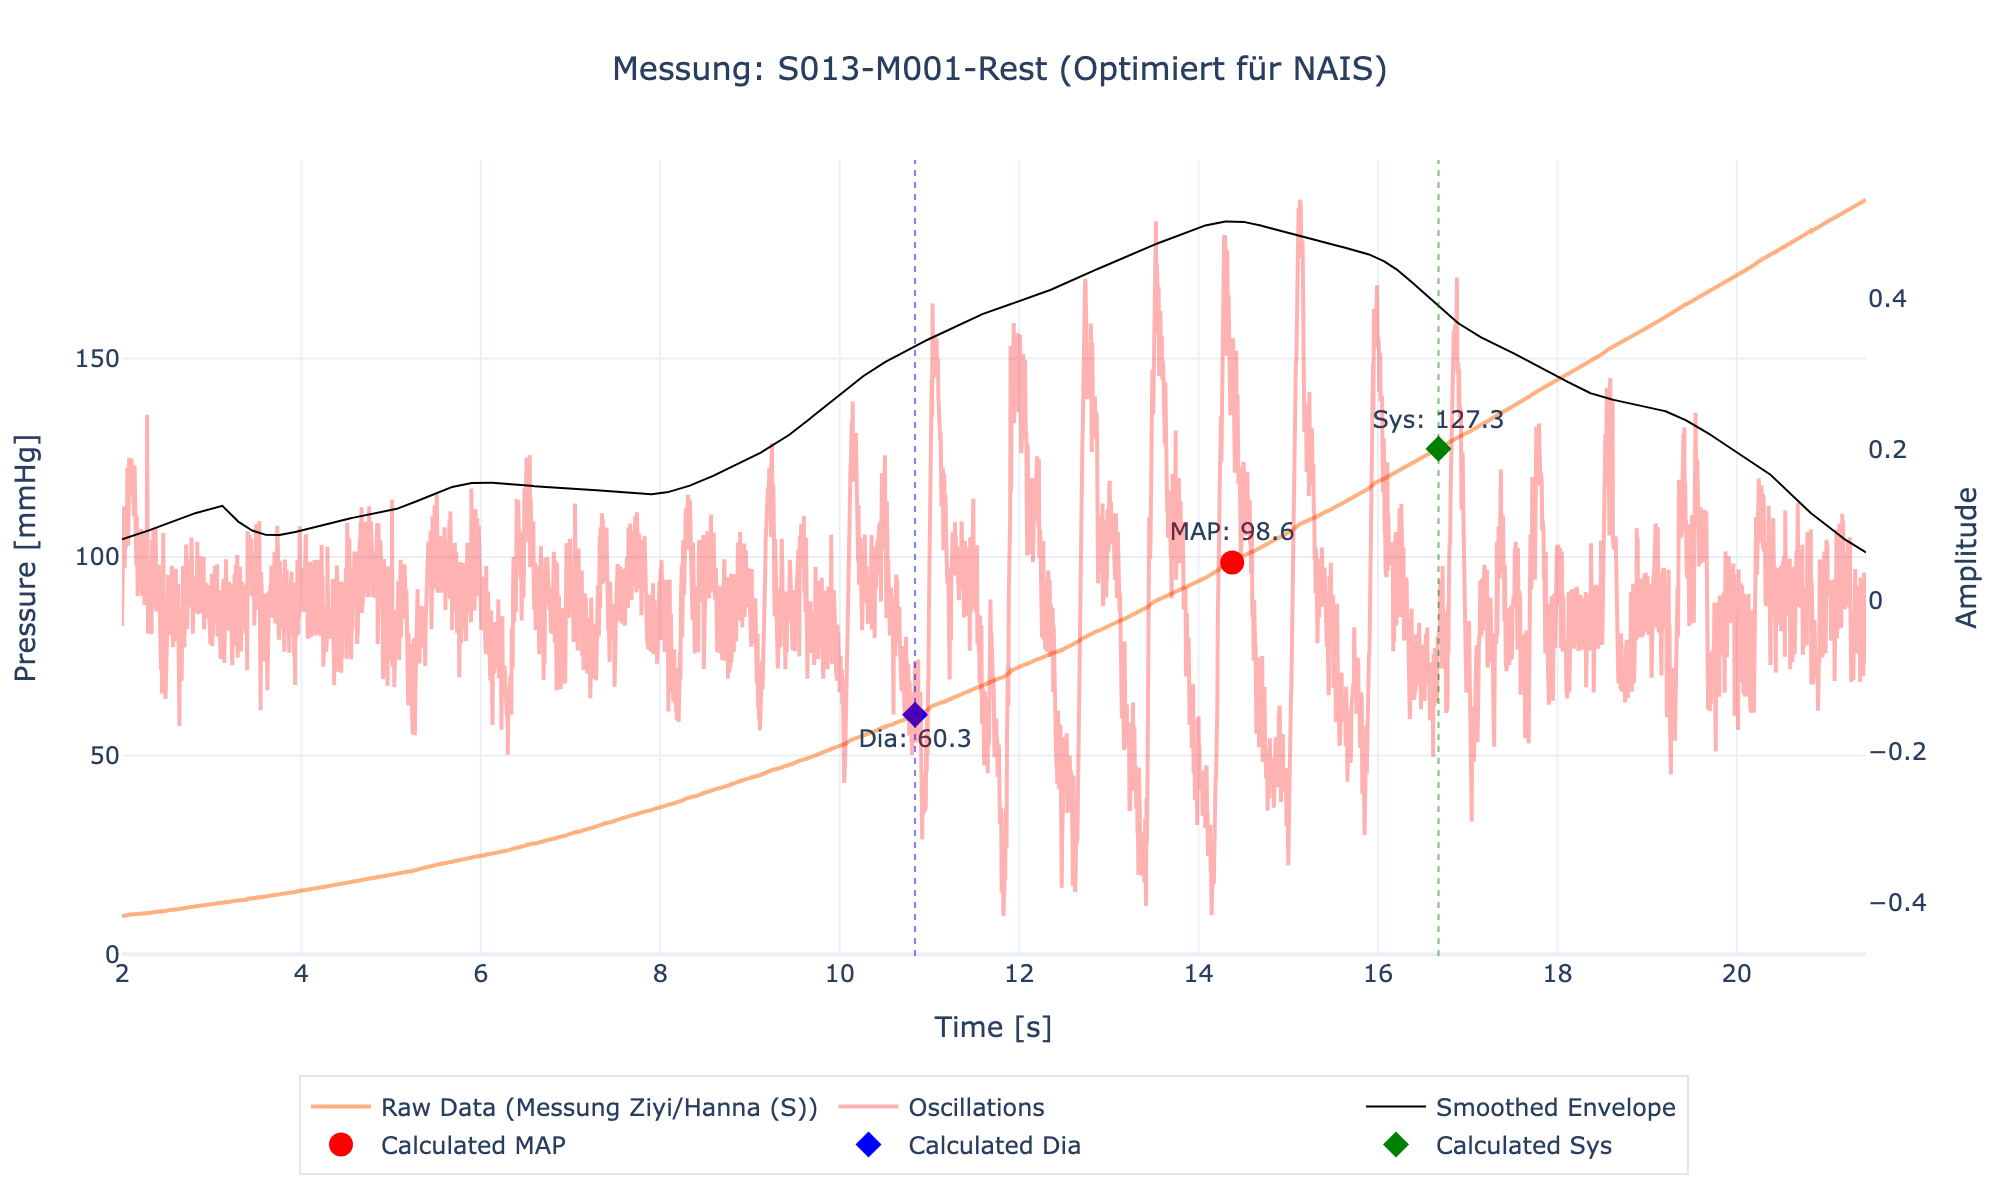
\includegraphics[width=\textwidth]{images/S013-M001-Rest_nais.png}
        \caption{Optimiert für NAIS}
    \end{subfigure}
    \caption{Einzelauswertung der Messung S013-M001-Rest mit verschiedenen Parametersätzen.}
\end{figure}
\newpage

\subsection*{Messung: S013-M002-Active}
\begin{figure}[H]
    \centering
    \begin{subfigure}[b]{0.8\textwidth}
        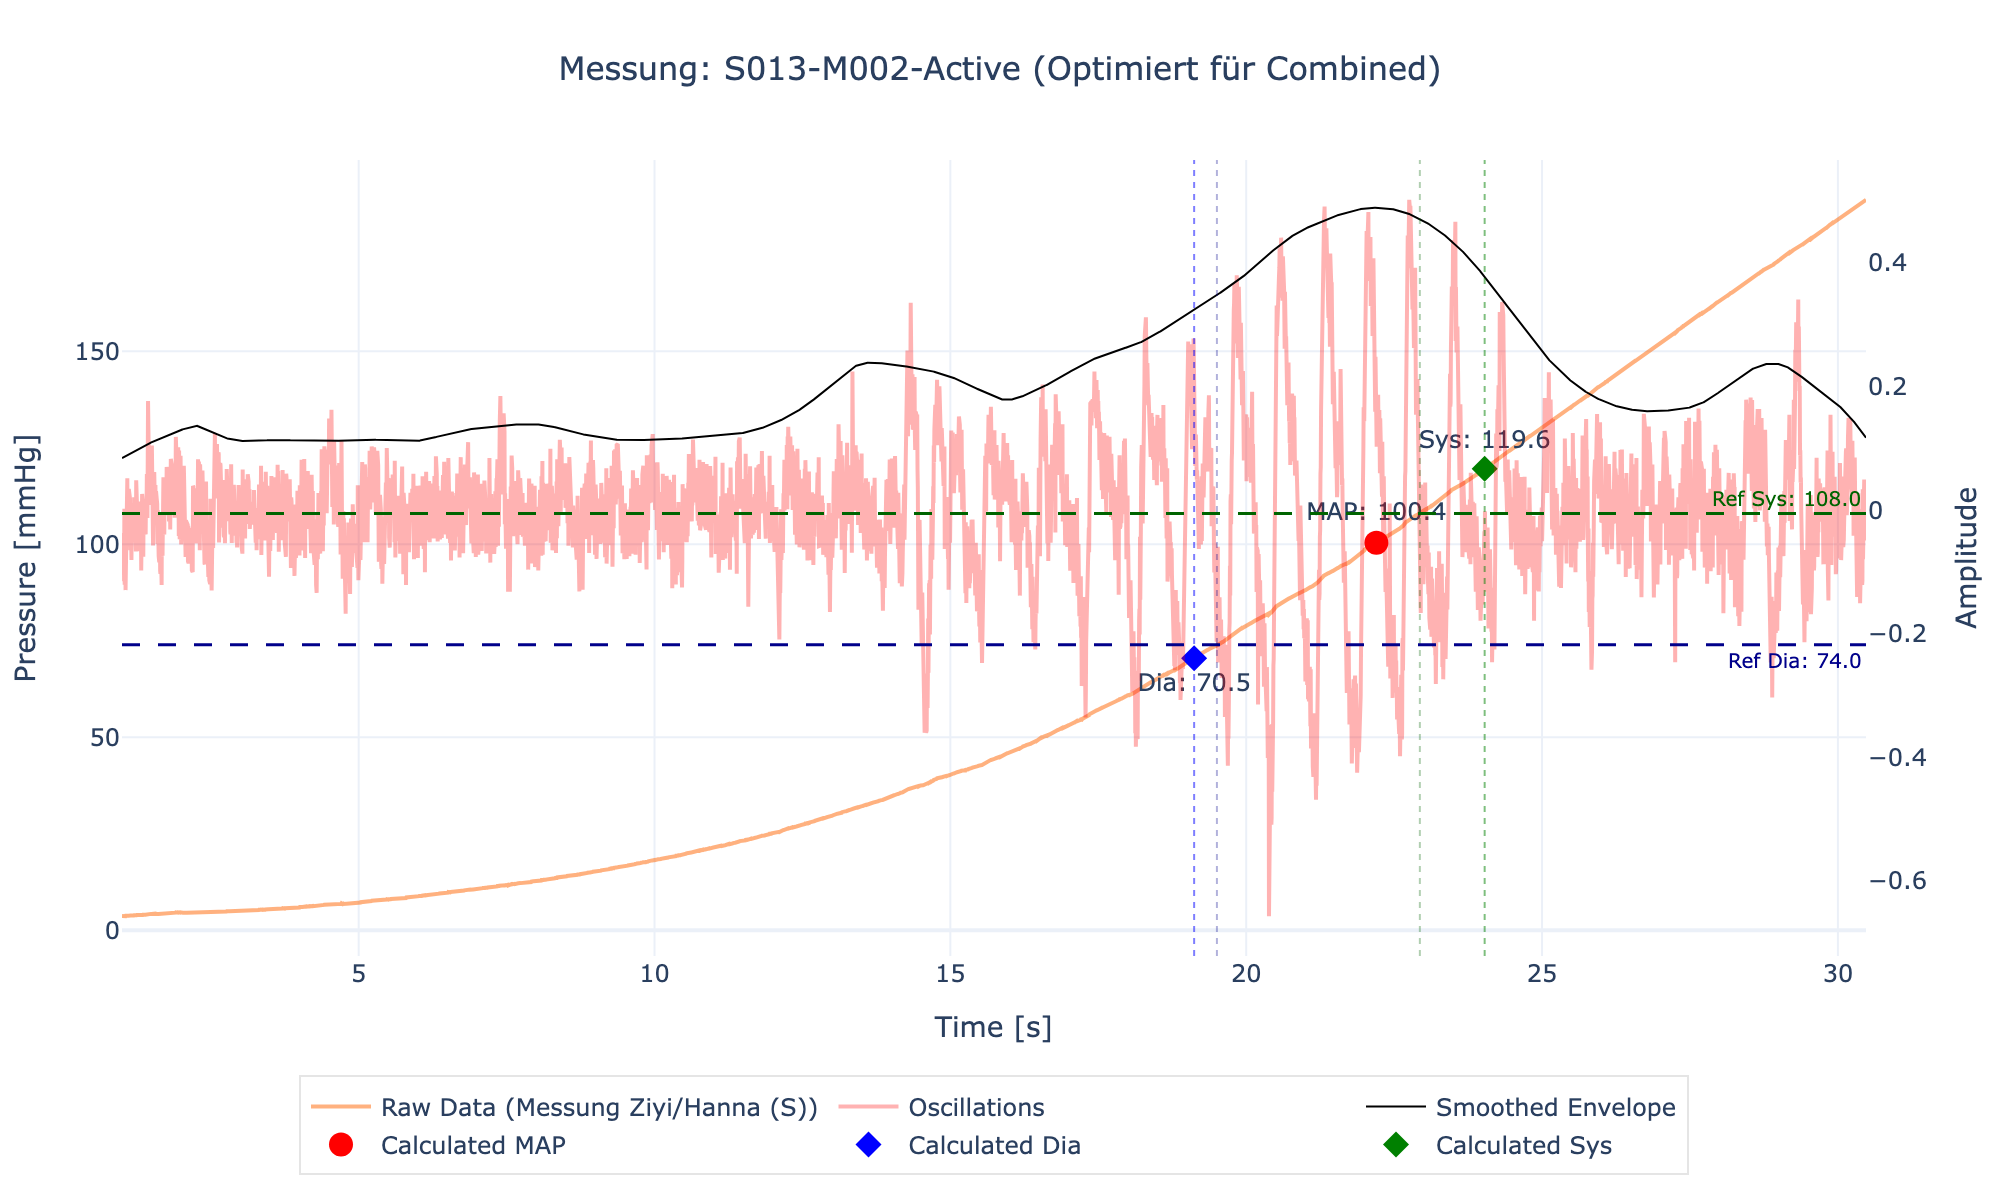
\includegraphics[width=\textwidth]{images/S013-M002-Active_combined.png}
        \caption{Optimiert für Beurer und NAIS (Kombiniert)}
    \end{subfigure} \\
    \begin{subfigure}[b]{0.48\textwidth}
        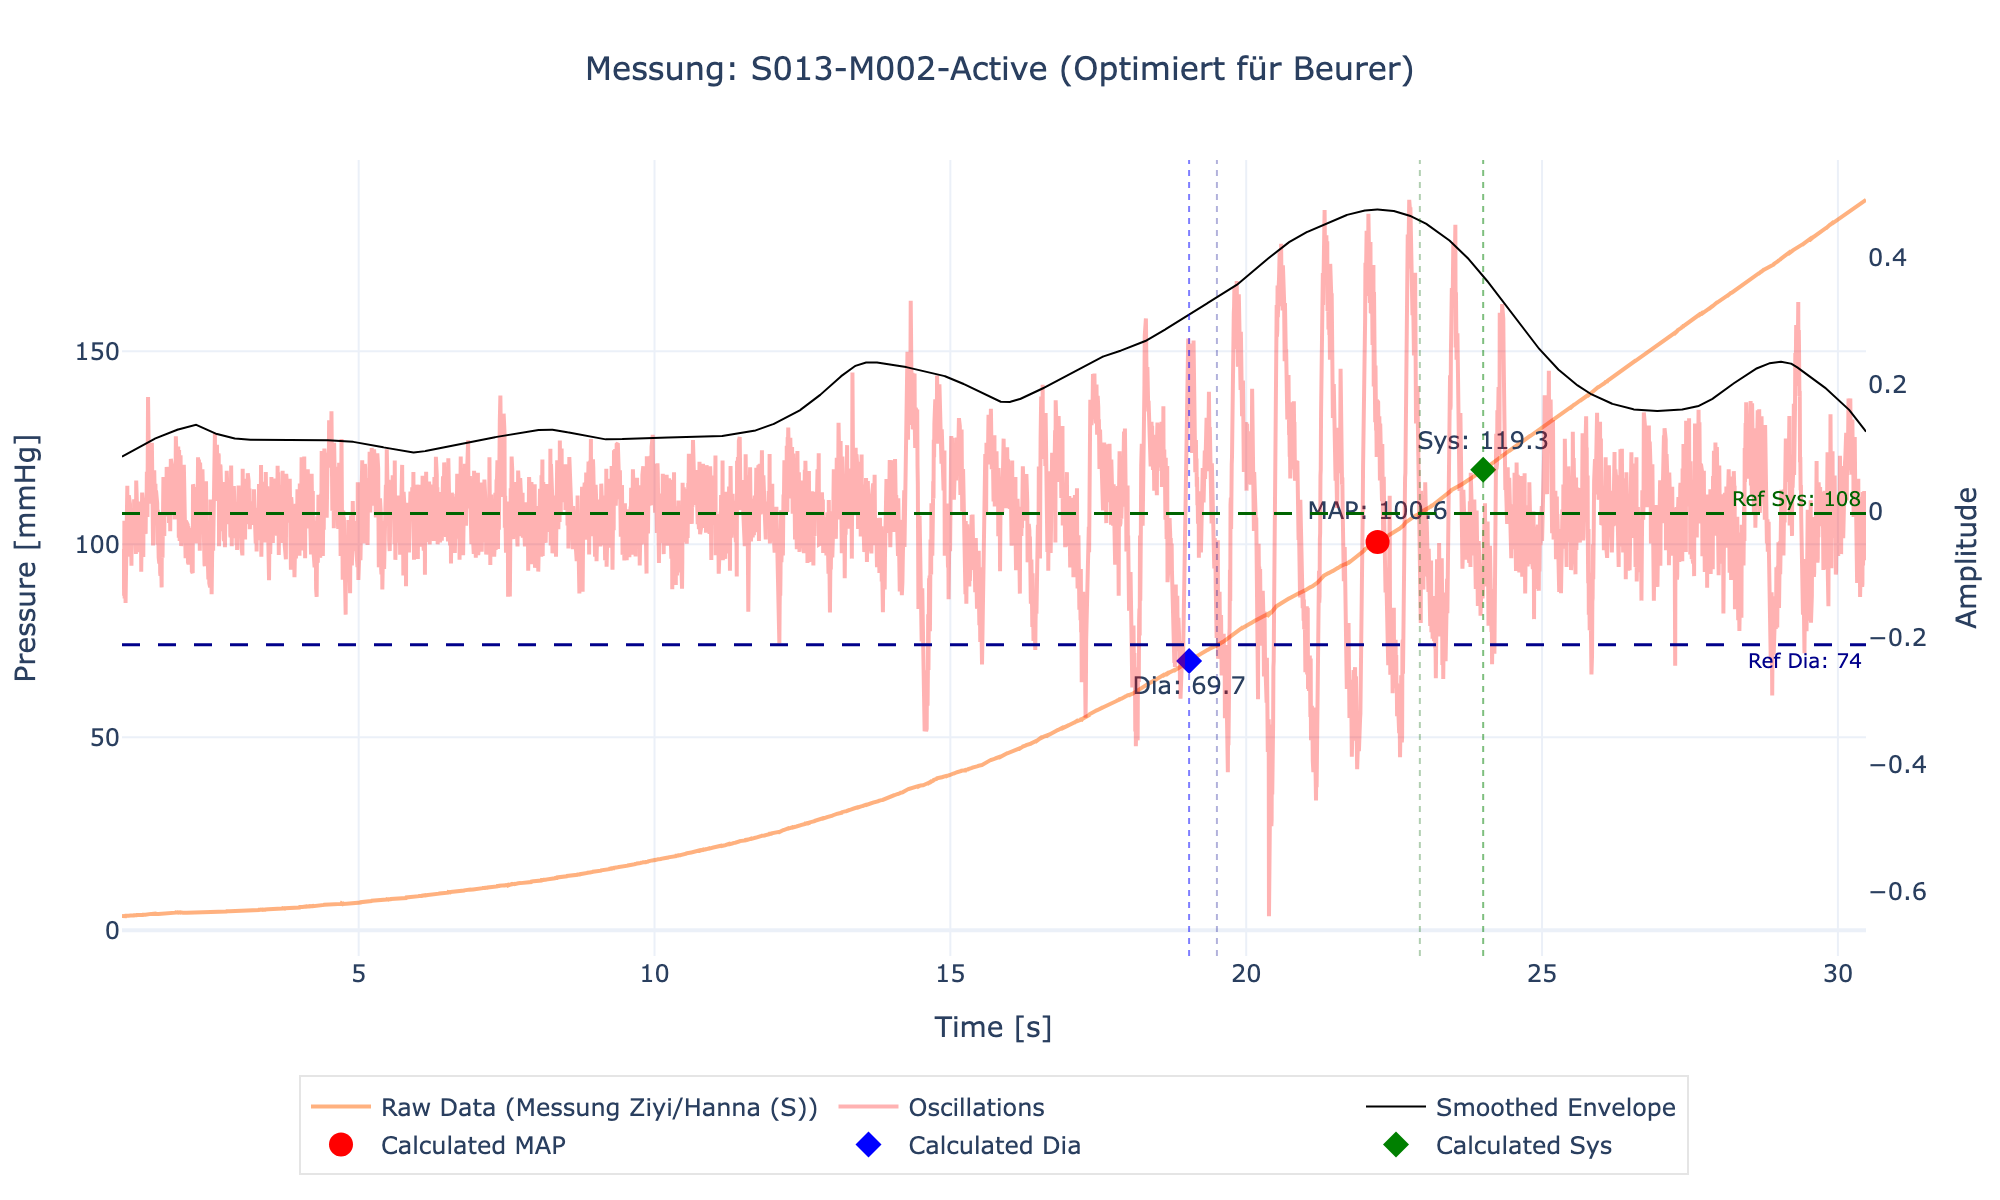
\includegraphics[width=\textwidth]{images/S013-M002-Active_beurer.png}
        \caption{Optimiert für Beurer}
    \end{subfigure}
    \hfill
    \begin{subfigure}[b]{0.48\textwidth}
        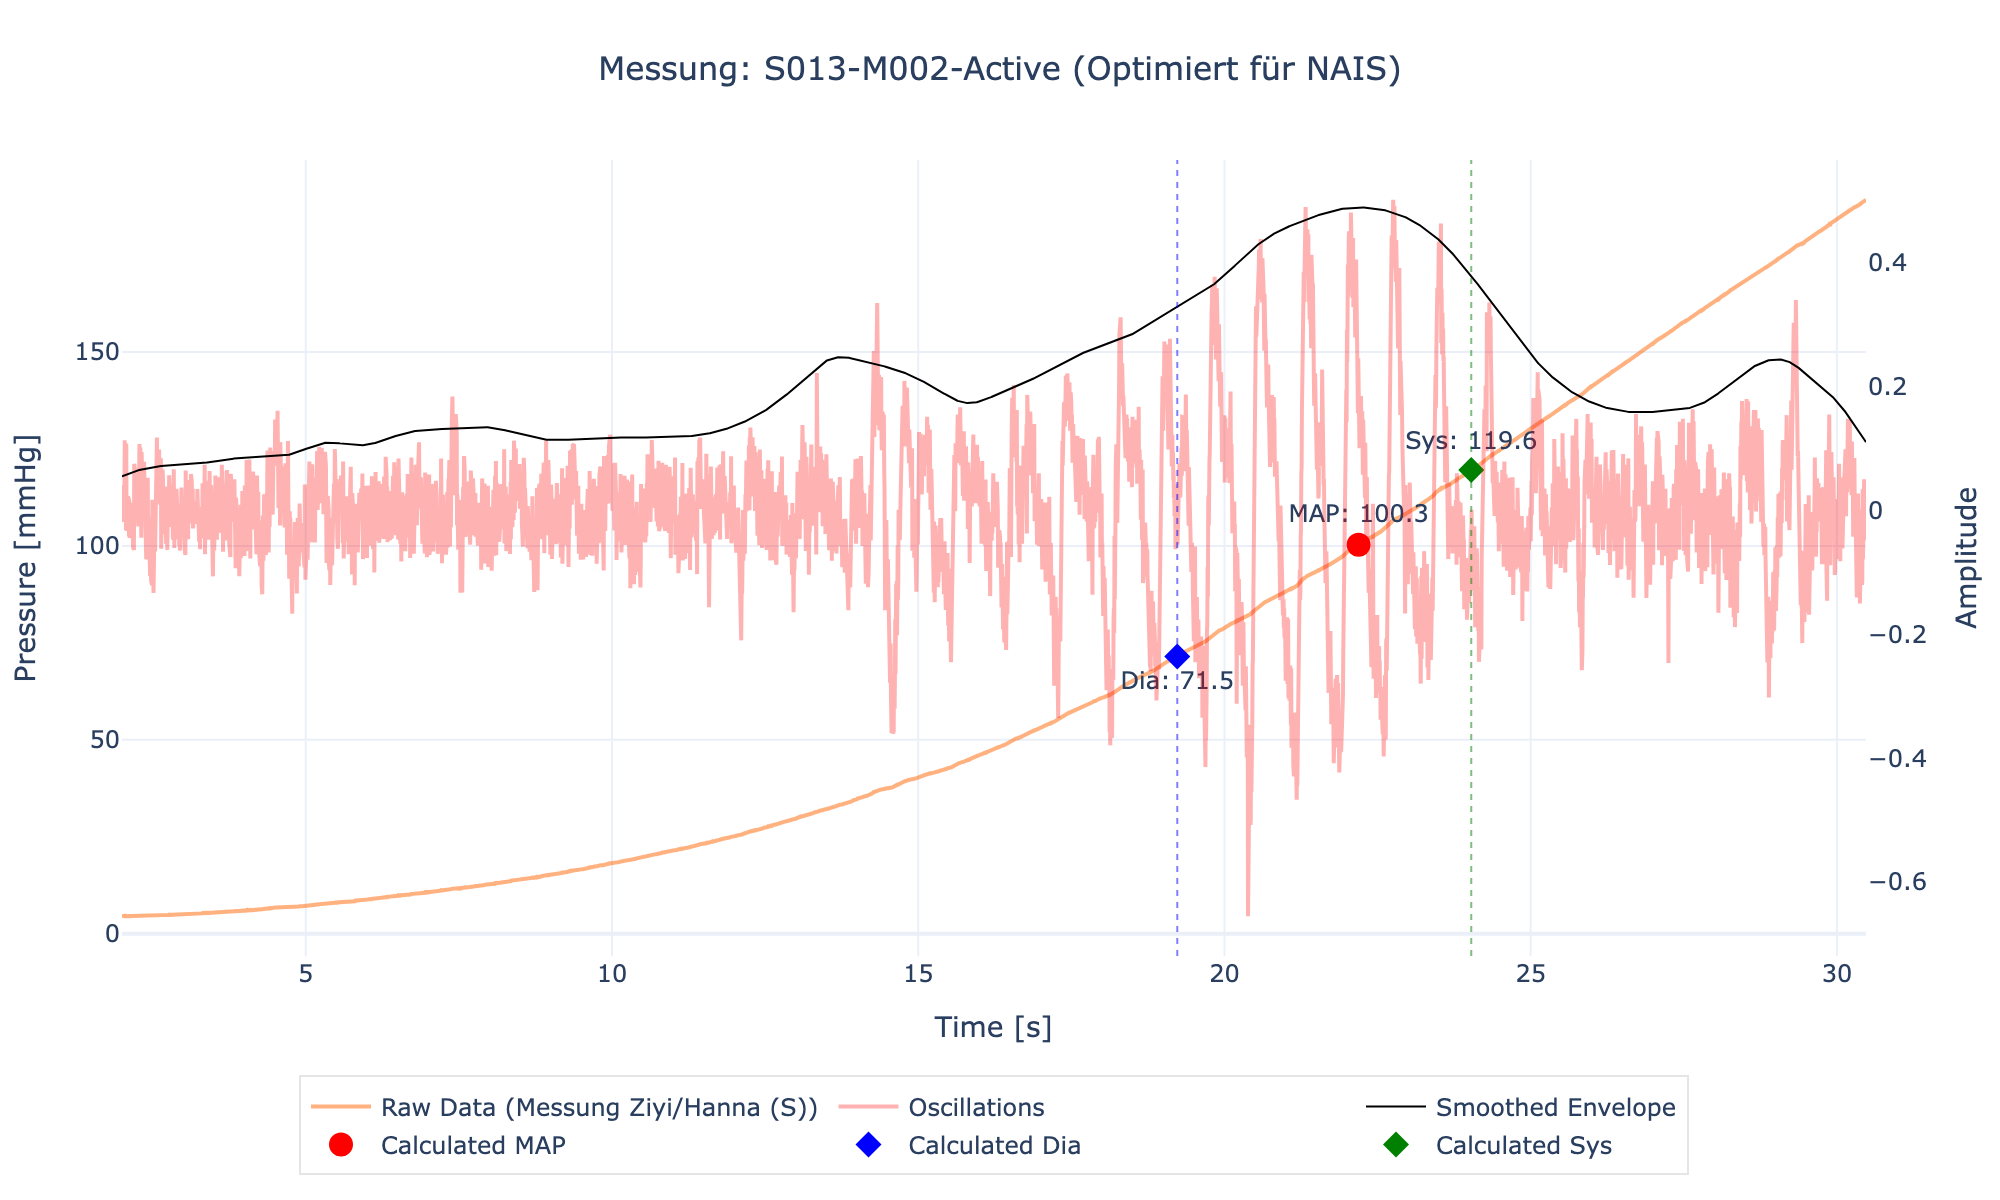
\includegraphics[width=\textwidth]{images/S013-M002-Active_nais.png}
        \caption{Optimiert für NAIS}
    \end{subfigure}
    \caption{Einzelauswertung der Messung S013-M002-Active mit verschiedenen Parametersätzen.}
\end{figure}
\newpage



\newpage

\section*{Empfindlichkeit gegenüber Signalstörungen}

\printbibliography

\end{document}